
% Indicate to rubber that there are external files
% rubber: shell_escape

\input{../Latex_Templates/Preamble_Report}

%%%%% TITLE PAGE

%\subject{, VT23}
\title{ Report for the Course Modelling in Computational Science, HT23 \\[1ex]
	  \large Project 2: Cell reprogramming}
%\subtitle{}
\author{Theo Koppenhöfer \\[1ex] (with Jimmy Gunnarson)}
\date{Lund \\[1ex] \today}

\addbibresource{bibliography.bib}

\usepackage{pythonhighlight}
\usepackage{pgfplots}
\graphicspath{{../Plots/}}

\pgfplotsset{
	compat=newest,
    every axis/.append style={
        axis y line=left,
        axis x line=bottom,
        scale only axis,
%    	max space between ticks=25pt,
        width=0.7\textwidth,
        scaled ticks=true,
        axis line style={thick,-,>=latex, shorten >=-.4cm},
    		x tick label style={
		    /pgf/number format/precision=3
		}
    },
    every axis plot/.append style={thick},
    tick style={black, thick}
}

%%%%% The content starts here %%%%%%%%%%%%%


\begin{document}

\maketitle

\section{Introduction}

\section{The setup}

\section{The experiments}

%\begin{figure}
%\begin{minipage}[t]{0.3\textwidth}
%\centering
%\graphicspath{{../Plots/}}
%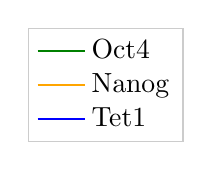
\begin{tikzpicture}

\definecolor{darkgray176}{RGB}{176,176,176}
\definecolor{gray}{RGB}{128,128,128}
\definecolor{green}{RGB}{0,128,0}
\definecolor{lightgray204}{RGB}{204,204,204}
\definecolor{orange}{RGB}{255,165,0}

\begin{axis}[
hide axis,
    xmin=10,
    xmax=50,
    ymin=0,
    ymax=0.4,
legend cell align={left},
legend style={fill opacity=0.8, draw opacity=1, text opacity=1, draw=lightgray204}
]

\addlegendimage{green}
\addlegendentry{Oct4};

\addlegendimage{orange}
\addlegendentry{Nanog};

\addlegendimage{blue}
\addlegendentry{Tet1};
\end{axis}

\end{tikzpicture}

%\caption{Varying Oct4.}
%\label{pl:Oct4}
%\end{minipage}
%\end{figure}


\begin{figure}
\begin{minipage}{\textwidth}
\centering
\begin{minipage}[t]{0.3\textwidth}
\centering
\graphicspath{{../Plots/}}
% This file was created with tikzplotlib v0.10.1.
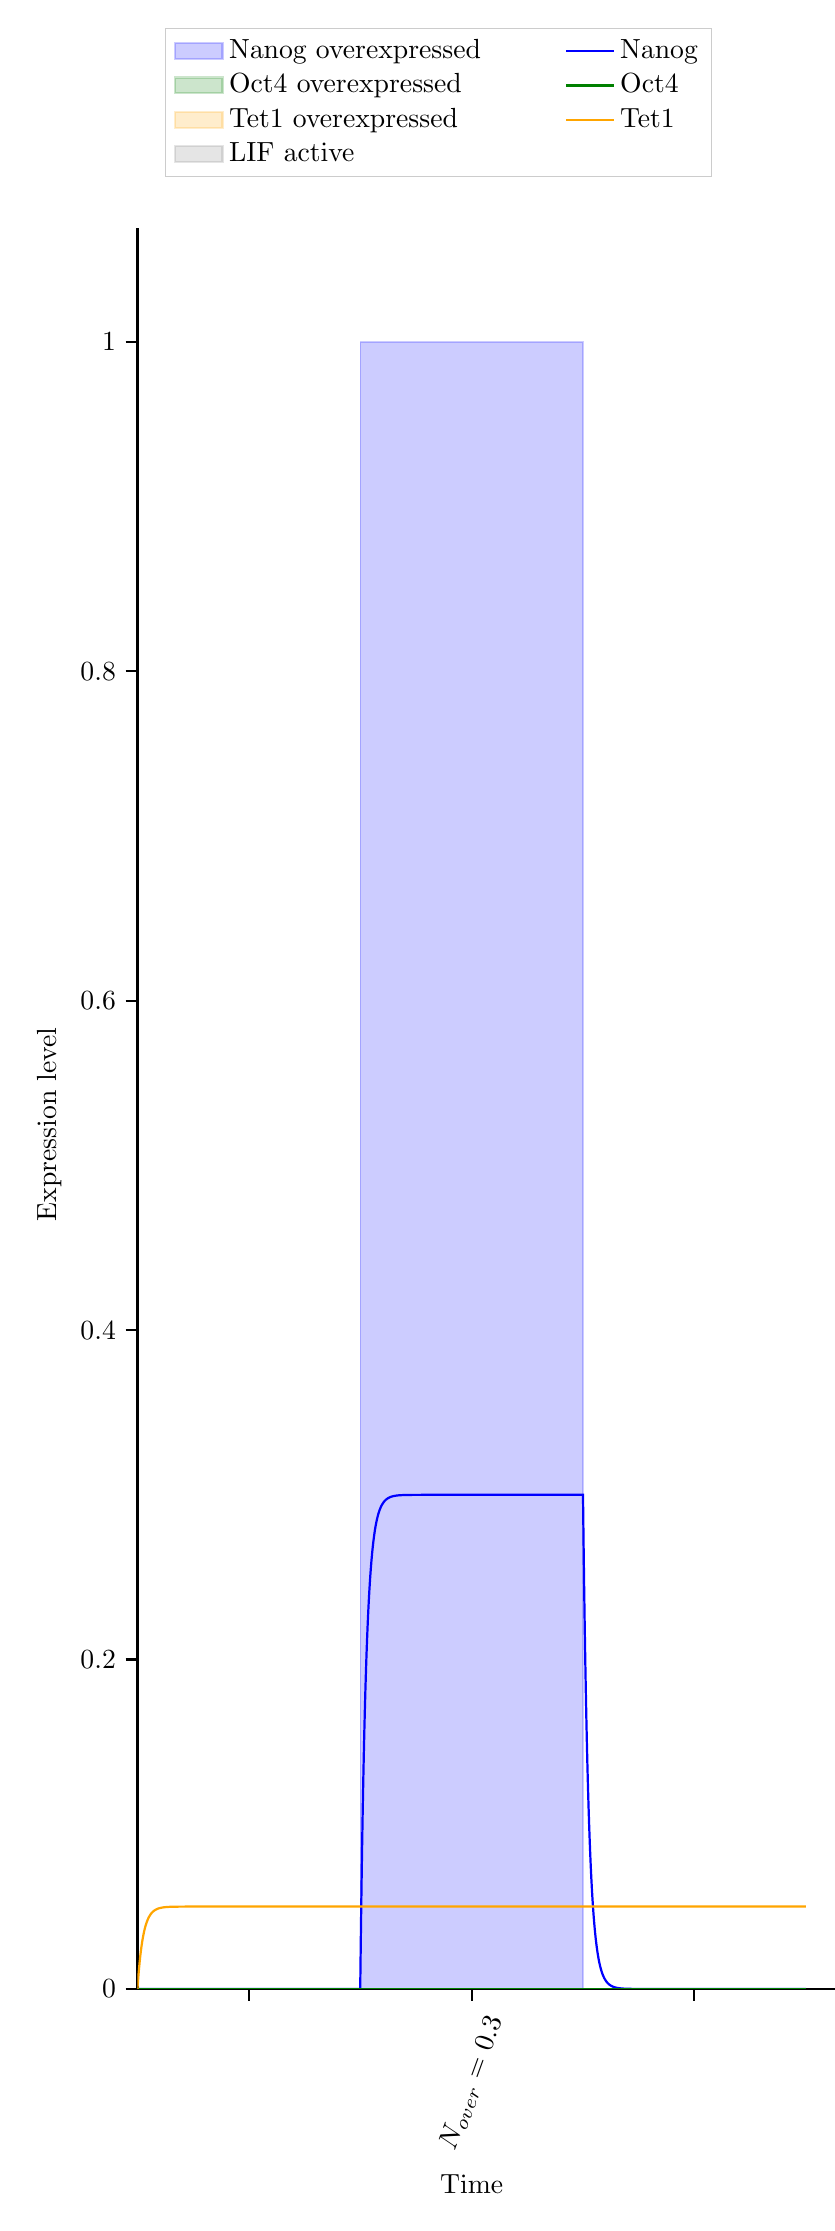
\begin{tikzpicture}[baseline]

\definecolor{darkgray176}{RGB}{176,176,176}
\definecolor{green}{RGB}{0,128,0}
\definecolor{lightgray204}{RGB}{204,204,204}
\definecolor{orange}{RGB}{255,165,0}

\begin{axis}[
 ytick={0,0.2,0.4,0.6,0.8,1},
 x tick label style = {rotate=70},
 y post scale=3, 
 transpose legend,
legend cell align={left},
legend style={fill opacity=0.8, draw opacity=1, text opacity=1, draw=lightgray204, anchor=south west,
    legend columns=4,
    /tikz/every even column/.append style={column sep=1.0cm},, at={(axis cs:5,1.1)}},
tick align=outside,
tick pos=left,
x grid style={darkgray176},
xlabel={Time},
xmin=0, xmax=120,
xtick style={color=black},
xtick={20,60,100},
xticklabels={,\(\displaystyle N_\text{over}=0.3\),},
y grid style={darkgray176},
ylabel={Expression level},
ymin=0, ymax=1.05,
ytick style={color=black}
]
\path [draw=blue, fill=blue, opacity=0.2]
(axis cs:40,0)
--(axis cs:40,1)
--(axis cs:80,1)
--(axis cs:80,0)
--cycle;
\addlegendimage{area legend, draw=blue, fill=blue, opacity=0.2}
\addlegendentry{Nanog overexpressed}
\addlegendimage{area legend, draw=green, fill=green, opacity=0.2}
\addlegendentry{Oct4 overexpressed}

\addlegendimage{area legend, draw=orange, fill=orange, opacity=0.2}
\addlegendentry{Tet1 overexpressed}

\addlegendimage{area legend, draw=gray, fill=gray, opacity=0.2}
\addlegendentry{LIF active}

\addplot [thick, blue]
table {%
0 0
0.0001 0
0.0011 0
0.0111 0
0.1111 0
0.2111 0
0.3111 0
0.4111 0
0.5111 0
0.6111 0
0.7111 0
0.8111 0
0.9111 0
1.0111 0
1.1111 0
1.2111 0
1.3111 0
1.4111 0
1.5111 0
1.6111 0
1.7111 0
1.8111 0
1.9111 0
2.0111 0
2.1111 0
2.2111 0
2.3111 0
2.4111 0
2.5111 0
2.6111 0
2.7111 0
2.8111 0
2.9111 0
3.0111 0
3.1111 0
3.2111 0
3.3111 0
3.4111 0
3.5111 0
3.6111 0
3.7111 0
3.8111 0
3.9111 0
4.0111 0
4.1111 0
4.2111 0
4.3111 0
4.4111 0
4.5111 0
4.6111 0
4.7111 0
4.8111 0
4.9111 0
5.0111 0
5.1111 0
5.2111 0
5.3111 0
5.4111 0
5.5111 0
5.6111 0
5.7111 0
5.8111 0
5.9111 0
6.0111 0
6.1111 0
6.21109999999999 0
6.31109999999999 0
6.41109999999999 0
6.51109999999999 0
6.61109999999999 0
6.71109999999999 0
6.81109999999999 0
6.91109999999999 0
7.01109999999999 0
7.11109999999999 0
7.21109999999999 0
7.31109999999999 0
7.41109999999999 0
7.51109999999999 0
7.61109999999999 0
7.71109999999999 0
7.81109999999999 0
7.91109999999999 0
8.01109999999999 0
8.11109999999999 0
8.21109999999999 0
8.31109999999999 0
8.41109999999999 0
8.51109999999999 0
8.61109999999999 0
8.71109999999999 0
8.81109999999999 0
8.91109999999999 0
9.01109999999998 0
9.11109999999998 0
9.21109999999998 0
9.31109999999998 0
9.41109999999998 0
9.51109999999998 0
9.61109999999998 0
9.71109999999998 0
9.81109999999998 0
9.91109999999998 0
10.0111 0
10.1111 0
10.2111 0
10.3111 0
10.4111 0
10.5111 0
10.6111 0
10.7111 0
10.8111 0
10.9111 0
11.0111 0
11.1111 0
11.2111 0
11.3111 0
11.4111 0
11.5111 0
11.6111 0
11.7111 0
11.8111 0
11.9111 0
12.0111 0
12.1111 0
12.2111 0
12.3111 0
12.4111 0
12.5111 0
12.6111 0
12.7111 0
12.8111 0
12.9111 0
13.0111 0
13.1111 0
13.2111 0
13.3111 0
13.4111 0
13.5111 0
13.6111 0
13.7111 0
13.8111 0
13.9111 0
14.0111 0
14.1111 0
14.2111 0
14.3111 0
14.4111 0
14.5111 0
14.6111 0
14.7111 0
14.8111 0
14.9111 0
15.0111 0
15.1111 0
15.2111 0
15.3111 0
15.4111 0
15.5111 0
15.6111 0
15.7111 0
15.8111 0
15.9111 0
16.0111 0
16.1111 0
16.2111 0
16.3111 0
16.4111 0
16.5111 0
16.6111 0
16.7111 0
16.8111 0
16.9111 0
17.0111 0
17.1111 0
17.2111 0
17.3111 0
17.4111 0
17.5111 0
17.6111 0
17.7111 0
17.8111 0
17.9111 0
18.0111 0
18.1111 0
18.2111 0
18.3111 0
18.4111 0
18.5111 0
18.6111 0
18.7111 0
18.8111 0
18.9111 0
19.0111 0
19.1111 0
19.2111 0
19.3111 0
19.4111 0
19.5111 0
19.6111 0
19.7111 0
19.8111 0
19.9111 0
20.0111 0
20.1111 0
20.2111 0
20.3111 0
20.4111 0
20.5111 0
20.6111 0
20.7111 0
20.8111 0
20.9111 0
21.0111 0
21.1111 0
21.2111 0
21.3111 0
21.4111 0
21.5111 0
21.6111 0
21.7111 0
21.8111 0
21.9111 0
22.0111 0
22.1111 0
22.2111 0
22.3111 0
22.4111000000001 0
22.5111000000001 0
22.6111000000001 0
22.7111000000001 0
22.8111000000001 0
22.9111000000001 0
23.0111000000001 0
23.1111000000001 0
23.2111000000001 0
23.3111000000001 0
23.4111000000001 0
23.5111000000001 0
23.6111000000001 0
23.7111000000001 0
23.8111000000001 0
23.9111000000001 0
24.0111000000001 0
24.1111000000001 0
24.2111000000001 0
24.3111000000001 0
24.4111000000001 0
24.5111000000001 0
24.6111000000001 0
24.7111000000001 0
24.8111000000001 0
24.9111000000001 0
25.0111000000001 0
25.1111000000001 0
25.2111000000001 0
25.3111000000001 0
25.4111000000001 0
25.5111000000001 0
25.6111000000001 0
25.7111000000001 0
25.8111000000001 0
25.9111000000001 0
26.0111000000001 0
26.1111000000001 0
26.2111000000001 0
26.3111000000001 0
26.4111000000001 0
26.5111000000001 0
26.6111000000001 0
26.7111000000001 0
26.8111000000001 0
26.9111000000001 0
27.0111000000001 0
27.1111000000001 0
27.2111000000001 0
27.3111000000001 0
27.4111000000001 0
27.5111000000001 0
27.6111000000001 0
27.7111000000001 0
27.8111000000001 0
27.9111000000001 0
28.0111000000001 0
28.1111000000001 0
28.2111000000001 0
28.3111000000001 0
28.4111000000001 0
28.5111000000001 0
28.6111000000001 0
28.7111000000001 0
28.8111000000001 0
28.9111000000001 0
29.0111000000001 0
29.1111000000001 0
29.2111000000001 0
29.3111000000001 0
29.4111000000002 0
29.5111000000002 0
29.6111000000002 0
29.7111000000002 0
29.8111000000002 0
29.9111000000002 0
30.0111000000002 0
30.1111000000002 0
30.2111000000002 0
30.3111000000002 0
30.4111000000002 0
30.5111000000002 0
30.6111000000002 0
30.7111000000002 0
30.8111000000002 0
30.9111000000002 0
31.0111000000002 0
31.1111000000002 0
31.2111000000002 0
31.3111000000002 0
31.4111000000002 0
31.5111000000002 0
31.6111000000002 0
31.7111000000002 0
31.8111000000002 0
31.9111000000002 0
32.0111000000002 0
32.1111000000002 0
32.2111000000002 0
32.3111000000002 0
32.4111000000002 0
32.5111000000002 0
32.6111000000002 0
32.7111000000002 0
32.8111000000002 0
32.9111000000002 0
33.0111000000002 0
33.1111000000002 0
33.2111000000002 0
33.3111000000002 0
33.4111000000002 0
33.5111000000002 0
33.6111000000002 0
33.7111000000002 0
33.8111000000002 0
33.9111000000002 0
34.0111000000002 0
34.1111000000002 0
34.2111000000002 0
34.3111000000002 0
34.4111000000002 0
34.5111000000002 0
34.6111000000002 0
34.7111000000002 0
34.8111000000002 0
34.9111000000002 0
35.0111000000002 0
35.1111000000002 0
35.2111000000002 0
35.3111000000002 0
35.4111000000002 0
35.5111000000002 0
35.6111000000002 0
35.7111000000002 0
35.8111000000002 0
35.9111000000002 0
36.0111000000002 0
36.1111000000002 0
36.2111000000002 0
36.3111000000002 0
36.4111000000002 0
36.5111000000002 0
36.6111000000002 0
36.7111000000003 0
36.8111000000003 0
36.9111000000003 0
37.0111000000003 0
37.1111000000003 0
37.2111000000003 0
37.3111000000003 0
37.4111000000003 0
37.5111000000003 0
37.6111000000003 0
37.7111000000003 0
37.8111000000003 0
37.9111000000003 0
38.0111000000003 0
38.1111000000003 0
38.2111000000003 0
38.3111000000003 0
38.4111000000003 0
38.5111000000003 0
38.6111000000003 0
38.7111000000003 0
38.8111000000003 0
38.9111000000003 0
39.0111000000003 0
39.1111000000003 0
39.2111000000003 0
39.3111000000003 0
39.4111000000003 0
39.5111000000003 0
39.6111000000003 0
39.7111000000003 0
39.8111000000003 0
39.9111000000003 0
40 0
40 0
40.0032679738562 0.000978791952511147
40.0359477124183 0.0105927799469138
40.1359477124183 0.0381335181601389
40.2359477124183 0.0630534086239877
40.3359477124183 0.0856018579764461
40.4359477124183 0.106004538675944
40.5359477124183 0.124465647607158
40.6359477124183 0.141169949752047
40.7359477124183 0.156284627379889
40.8359477124183 0.169960953263606
40.9359477124183 0.182335804668514
41.0359477124183 0.193533033265989
41.1359477124183 0.203664704682617
41.2359477124183 0.21283222009064
41.3359477124183 0.221127331064966
41.4359477124183 0.228633057863765
41.5359477124183 0.235424520323105
41.6359477124183 0.241569689681521
41.7359477124183 0.247130068859012
41.8359477124183 0.252161307998928
41.9359477124183 0.256713761433306
42.0359477124183 0.260832991645952
42.1359477124183 0.264560225277083
42.2359477124184 0.267932765733401
42.3359477124184 0.270984366533121
42.4359477124184 0.273745569122523
42.5359477124184 0.276244008545012
42.6359477124184 0.27850469002192
42.7359477124184 0.28055023921316
42.8359477124184 0.282401128662435
42.9359477124184 0.284075882693337
43.0359477124184 0.285591262807002
43.1359477124184 0.286962435436844
43.2359477124184 0.28820312373932
43.3359477124184 0.289325744939888
43.4359477124184 0.290341534608777
43.5359477124184 0.291260659110344
43.6359477124184 0.292092317351469
43.7359477124184 0.292844832847304
43.8359477124184 0.293525737025811
43.9359477124184 0.294141844604824
44.0359477124184 0.294699321796033
44.1359477124184 0.295203748018507
44.2359477124184 0.29566017173939
44.3359477124184 0.296073161000659
44.4359477124184 0.296446849137626
44.5359477124184 0.296784976146741
44.6359477124184 0.297090926116737
44.7359477124184 0.297367761097727
44.8359477124184 0.297618251747231
44.9359477124184 0.297844905059844
45.0359477124184 0.298049989458086
45.1359477124184 0.298235557495532
45.2359477124184 0.29840346639946
45.3359477124184 0.298555396658605
45.4359477124184 0.298692868842056
45.5359477124184 0.298817258817623
45.6359477124184 0.298929811521982
45.7359477124184 0.29903165342042
45.8359477124184 0.299123803780881
45.9359477124184 0.299207184875139
46.0359477124184 0.299282631209205
46.1359477124184 0.299350897875344
46.2359477124184 0.299412668109292
46.3359477124184 0.299468560128307
46.4359477124184 0.299519133318497
46.5359477124184 0.299564893833347
46.6359477124184 0.299606299659465
46.7359477124184 0.299643765200273
46.8359477124184 0.299677665423495
46.9359477124184 0.299708339613955
47.0359477124184 0.299736094769261
47.1359477124184 0.299761208672334
47.2359477124184 0.299783932671554
47.3359477124184 0.299804494196343
47.4359477124184 0.29982309903335
47.5359477124184 0.299839933386035
47.6359477124184 0.299855165738259
47.7359477124184 0.29986894854052
47.8359477124184 0.299881419735735
47.9359477124184 0.299892704139817
48.0359477124184 0.299902914690874
48.1359477124184 0.299912153579533
48.2359477124184 0.299920513271695
48.3359477124184 0.299928077433968
48.4359477124184 0.299934921771032
48.5359477124184 0.299941114783311
48.6359477124184 0.299946718452553
48.7359477124184 0.299951788862163
48.8359477124184 0.299956376758505
48.9359477124184 0.299960528058786
49.0359477124184 0.299964284310616
49.1359477124184 0.299967683107823
49.2359477124185 0.299970758466714
49.3359477124185 0.299973541166514
49.4359477124185 0.299976059057416
49.5359477124185 0.29997833733932
49.6359477124185 0.299980398814036
49.7359477124185 0.299982264113496
49.8359477124185 0.299983951906244
49.9359477124185 0.299985479084277
50.0359477124185 0.299986860932105
50.1359477124185 0.299988111279727
50.2359477124185 0.29998924264104
50.3359477124185 0.299990266339091
50.4359477124185 0.299991192619392
50.5359477124185 0.299992030752469
50.6359477124185 0.299992789126638
50.7359477124185 0.299993475331963
50.8359477124185 0.299994096236218
50.9359477124185 0.299994658053621
51.0359477124185 0.299995166407029
51.1359477124185 0.299995626384215
51.2359477124185 0.299996042588784
51.3359477124185 0.299996419186252
51.4359477124185 0.299996759945733
51.5359477124185 0.299997068277662
51.6359477124185 0.299997347267928
51.7359477124185 0.299997599708761
51.8359477124185 0.299997828126672
51.9359477124185 0.299998034807745
52.0359477124185 0.299998221820513
52.1359477124185 0.299998391036664
52.2359477124185 0.299998544149769
52.3359477124185 0.299998682692235
52.4359477124185 0.299998808050643
52.5359477124185 0.299998921479621
52.6359477124185 0.299999024114405
52.7359477124185 0.299999116982197
52.8359477124185 0.299999201012451
52.9359477124185 0.299999277046169
53.0359477124185 0.299999345844322
53.1359477124185 0.299999408095465
53.2359477124185 0.299999464422629
53.3359477124185 0.299999515389554
53.4359477124185 0.299999561506335
53.5359477124185 0.299999603234524
53.6359477124185 0.299999640991751
53.7359477124185 0.299999675155903
53.8359477124185 0.299999706068906
53.9359477124185 0.299999734040148
54.0359477124185 0.299999759349574
54.1359477124185 0.29999978225049
54.2359477124185 0.299999802972095
54.3359477124185 0.299999821721779
54.4359477124185 0.299999838687195
54.5359477124185 0.299999854038138
54.6359477124185 0.299999867928246
54.7359477124185 0.299999880496535
54.8359477124185 0.299999891868793
54.9359477124185 0.299999902158838
55.0359477124185 0.299999911469655
55.1359477124185 0.299999919894432
55.2359477124185 0.299999927517484
55.3359477124185 0.299999934415108
55.4359477124185 0.299999940656335
55.5359477124185 0.299999946303632
55.6359477124185 0.299999951413517
55.7359477124185 0.299999956037132
55.8359477124185 0.299999960220752
55.9359477124185 0.299999964006248
56.0359477124185 0.299999967431506
56.1359477124185 0.299999970530808
56.2359477124186 0.299999973335172
56.3359477124186 0.299999975872666
56.4359477124186 0.299999978168686
56.5359477124186 0.29999998024621
56.6359477124186 0.299999982126032
56.7359477124186 0.299999983826965
56.8359477124186 0.299999985366032
56.9359477124186 0.299999986758639
57.0359477124186 0.299999988018721
57.1359477124186 0.29999998915889
57.2359477124186 0.299999990190558
57.3359477124186 0.29999999112405
57.4359477124186 0.299999991968708
57.5359477124186 0.299999992732987
57.6359477124186 0.299999993424534
57.7359477124186 0.299999994050273
57.8359477124186 0.299999994616464
57.9359477124186 0.299999995128775
58.0359477124186 0.299999995592334
58.1359477124186 0.299999996011779
58.2359477124186 0.299999996391308
58.3359477124186 0.29999999673472
58.4359477124186 0.299999997045453
58.5359477124186 0.299999997326615
58.6359477124186 0.299999997581021
58.7359477124186 0.299999997811218
58.8359477124186 0.299999998019508
58.9359477124186 0.299999998207977
59.0359477124186 0.29999999837851
59.1359477124186 0.299999998532815
59.2359477124186 0.299999998672436
59.3359477124186 0.299999998798771
59.4359477124186 0.299999998913083
59.5359477124186 0.299999999016517
59.6359477124186 0.299999999110107
59.7359477124186 0.299999999194792
59.8359477124186 0.299999999271418
59.9359477124186 0.299999999340751
60.0359477124186 0.299999999403487
60.1359477124186 0.299999999460253
60.2359477124186 0.299999999511617
60.3359477124186 0.299999999558092
60.4359477124186 0.299999999600146
60.5359477124186 0.299999999638197
60.6359477124186 0.299999999672627
60.7359477124186 0.299999999703781
60.8359477124186 0.29999999973197
60.9359477124186 0.299999999757476
61.0359477124186 0.299999999780555
61.1359477124186 0.299999999801438
61.2359477124186 0.299999999820334
61.3359477124186 0.299999999837431
61.4359477124186 0.299999999852902
61.5359477124186 0.2999999998669
61.6359477124186 0.299999999879566
61.7359477124186 0.299999999891027
61.8359477124186 0.299999999901397
61.9359477124186 0.29999999991078
62.0359477124186 0.299999999919271
62.1359477124186 0.299999999926953
62.2359477124186 0.299999999933905
62.3359477124186 0.299999999940194
62.4359477124186 0.299999999945886
62.5359477124186 0.299999999951035
62.6359477124186 0.299999999955695
62.7359477124186 0.299999999959911
62.8359477124186 0.299999999963726
62.9359477124186 0.299999999967178
63.0359477124186 0.299999999970301
63.1359477124186 0.299999999973128
63.2359477124186 0.299999999975685
63.3359477124187 0.299999999977999
63.4359477124187 0.299999999980092
63.5359477124187 0.299999999981987
63.6359477124187 0.299999999983701
63.7359477124187 0.299999999985252
63.8359477124187 0.299999999986655
63.9359477124187 0.299999999987925
64.0359477124187 0.299999999989074
64.1359477124187 0.299999999990114
64.2359477124186 0.299999999991055
64.3359477124186 0.299999999991906
64.4359477124186 0.299999999992676
64.5359477124186 0.299999999993373
64.6359477124186 0.299999999994004
64.7359477124186 0.299999999994574
64.8359477124186 0.299999999995091
64.9359477124186 0.299999999995558
65.0359477124186 0.299999999995981
65.1359477124186 0.299999999996363
65.2359477124186 0.299999999996709
65.3359477124186 0.299999999997022
65.4359477124186 0.299999999997306
65.5359477124186 0.299999999997562
65.6359477124186 0.299999999997794
65.7359477124186 0.299999999998004
65.8359477124186 0.299999999998194
65.9359477124186 0.299999999998366
66.0359477124185 0.299999999998521
66.1359477124185 0.299999999998662
66.2359477124185 0.299999999998789
66.3359477124185 0.299999999998905
66.4359477124185 0.299999999999009
66.5359477124185 0.299999999999103
66.6359477124185 0.299999999999189
66.7359477124185 0.299999999999266
66.8359477124185 0.299999999999336
66.9359477124185 0.299999999999399
67.0359477124185 0.299999999999456
67.1359477124185 0.299999999999508
67.2359477124185 0.299999999999555
67.3359477124185 0.299999999999597
67.4359477124185 0.299999999999635
67.5359477124185 0.29999999999967
67.6359477124185 0.299999999999702
67.7359477124185 0.29999999999973
67.8359477124184 0.299999999999756
67.9359477124184 0.299999999999779
68.0359477124184 0.2999999999998
68.1359477124184 0.299999999999819
68.2359477124184 0.299999999999836
68.3359477124184 0.299999999999852
68.4359477124184 0.299999999999866
68.5359477124184 0.299999999999879
68.6359477124184 0.29999999999989
68.7359477124184 0.299999999999901
68.8359477124184 0.29999999999991
68.9359477124184 0.299999999999919
69.0359477124184 0.299999999999926
69.1359477124184 0.299999999999933
69.2359477124184 0.29999999999994
69.3359477124184 0.299999999999945
69.4359477124184 0.299999999999951
69.5359477124183 0.299999999999955
69.6359477124183 0.29999999999996
69.7359477124183 0.299999999999963
69.8359477124183 0.299999999999967
69.9359477124183 0.29999999999997
70.0359477124183 0.299999999999973
70.1359477124183 0.299999999999975
70.2359477124183 0.299999999999978
70.3359477124183 0.29999999999998
70.4359477124183 0.299999999999982
70.5359477124183 0.299999999999984
70.6359477124183 0.299999999999985
70.7359477124183 0.299999999999986
70.8359477124183 0.299999999999988
70.9359477124183 0.299999999999989
71.0359477124183 0.29999999999999
71.1359477124183 0.299999999999991
71.2359477124183 0.299999999999992
71.3359477124182 0.299999999999993
71.4359477124182 0.299999999999993
71.5359477124182 0.299999999999994
71.6359477124182 0.299999999999994
71.7359477124182 0.299999999999995
71.8359477124182 0.299999999999995
71.9359477124182 0.299999999999996
72.0359477124182 0.299999999999996
72.1359477124182 0.299999999999997
72.2359477124182 0.299999999999997
72.3359477124182 0.299999999999997
72.4359477124182 0.299999999999998
72.5359477124182 0.299999999999998
72.6359477124182 0.299999999999998
72.7359477124182 0.299999999999998
72.8359477124182 0.299999999999998
72.9359477124182 0.299999999999998
73.0359477124181 0.299999999999999
73.1359477124181 0.299999999999999
73.2359477124181 0.299999999999999
73.3359477124181 0.299999999999999
73.4359477124181 0.299999999999999
73.5359477124181 0.299999999999999
73.6359477124181 0.299999999999999
73.7359477124181 0.299999999999999
73.8359477124181 0.299999999999999
73.9359477124181 0.299999999999999
74.0359477124181 0.299999999999999
74.1359477124181 0.3
74.2359477124181 0.3
74.3359477124181 0.3
74.4359477124181 0.3
74.5359477124181 0.3
74.6359477124181 0.3
74.7359477124181 0.3
74.835947712418 0.3
74.935947712418 0.3
75.035947712418 0.3
75.135947712418 0.3
75.235947712418 0.3
75.335947712418 0.3
75.435947712418 0.3
75.535947712418 0.3
75.635947712418 0.3
75.735947712418 0.3
75.835947712418 0.3
75.935947712418 0.3
76.035947712418 0.3
76.135947712418 0.3
76.235947712418 0.3
76.335947712418 0.3
76.435947712418 0.3
76.535947712418 0.3
76.6359477124179 0.3
76.7359477124179 0.3
76.8359477124179 0.3
76.9359477124179 0.3
77.0359477124179 0.3
77.1359477124179 0.3
77.2359477124179 0.3
77.3359477124179 0.3
77.4359477124179 0.3
77.5359477124179 0.3
77.6359477124179 0.3
77.7359477124179 0.3
77.8359477124179 0.3
77.9359477124179 0.3
78.0359477124179 0.3
78.1359477124179 0.3
78.2359477124179 0.3
78.3359477124178 0.3
78.4359477124178 0.3
78.5359477124178 0.3
78.6359477124178 0.3
78.7359477124178 0.3
78.8359477124178 0.3
78.9359477124178 0.3
79.0359477124178 0.3
79.1359477124178 0.3
79.2359477124178 0.3
79.3359477124178 0.3
79.4359477124178 0.3
79.5359477124178 0.3
79.6359477124178 0.3
79.7359477124178 0.3
79.8359477124178 0.3
79.9359477124178 0.3
80 0.3
80 0.3
80.1 0.271451225500001
80.2 0.245619226084842
80.3 0.222245466423641
80.4 0.201096014075056
80.5 0.181959198212798
80.6 0.164643491152873
80.7 0.148975591480153
80.8 0.134798689589584
80.8999999999999 0.121970898282956
80.9999999999999 0.110363832714148
81.0999999999999 0.0998613254704424
81.1999999999999 0.0903582639300203
81.2999999999999 0.081759538259522
81.3999999999999 0.0739790895228717
81.4999999999999 0.0669390483745262
81.5999999999999 0.0605689557168967
81.6999999999999 0.0548050575220231
81.7999999999999 0.0495896667598375
81.8999999999999 0.044870586046982
81.9999999999999 0.0406005852378551
82.0999999999999 0.0367369287294434
82.1999999999999 0.0332409477490455
82.2999999999999 0.0300776533441997
82.3999999999999 0.0272153862014907
82.4999999999999 0.0246254997895017
82.5999999999999 0.0222820736547008
82.6999999999998 0.0201616540008328
82.7999999999998 0.0182430189554436
82.8999999999998 0.0165069661742497
82.9999999999998 0.0149361206576239
83.0999999999998 0.0135147608557596
83.1999999999998 0.012228661322118
83.2999999999998 0.011064950340378
83.3999999999998 0.0100119810999742
83.4999999999998 0.00905921513090286
83.5999999999998 0.00819711683117246
83.6999999999998 0.00741705803129484
83.7999999999998 0.00671123164066538
83.8999999999998 0.00607257351157668
83.9999999999998 0.00549469173885446
84.0999999999998 0.00497180268752259
84.1999999999998 0.00449867310824069
84.2999999999998 0.00407056776118612
84.3999999999997 0.00368320202418257
84.4999999999997 0.00333269901076148
84.5999999999997 0.00301555076897949
84.6999999999997 0.00272858317265652
84.7999999999997 0.00246892415365431
84.8999999999997 0.00223397495725339
84.9999999999997 0.00202138413294249
85.0999999999997 0.00182902400031165
85.1999999999997 0.00165496935451171
85.2999999999997 0.00149747819815717
85.3999999999997 0.00135497430683099
85.4999999999997 0.00122603145370096
85.5999999999997 0.00110935913536225
85.6999999999997 0.00100378965604568
85.7999999999997 0.000908266440926083
85.8999999999997 0.000821833461566367
85.9999999999997 0.000743625667663662
86.0999999999997 0.000672860329335193
86.1999999999996 0.000608829203294576
86.2999999999996 0.000550891444515008
86.3999999999996 0.000498467192436883
86.4999999999996 0.000451031767528457
86.5999999999996 0.000408110420116771
86.6999999999996 0.000369273578933393
86.7999999999996 0.000334132551820804
86.8999999999996 0.000302335635570667
86.9999999999996 0.000273564595959931
87.0999999999996 0.000247531482755787
87.1999999999996 0.00022397574781297
87.2999999999996 0.000202661637420366
87.3999999999996 0.000183375832798651
87.4999999999996 0.000165925315134258
87.5999999999996 0.000150135433782227
87.6999999999996 0.000135848158303866
87.7999999999996 0.000122920496845009
87.8999999999996 0.000111223065025489
87.9999999999995 0.000100638791016785
88.0999999999995 9.10617438478159e-05
88.1999999999995 8.23960732121895e-05
88.2999999999995 7.45550501661223e-05
88.3999999999995 6.74601991160267e-05
88.4999999999995 6.10405124083985e-05
88.5999999999995 5.52317396613594e-05
88.6999999999995 4.99757447252435e-05
88.7999999999995 4.52199238364753e-05
88.8999999999995 4.09166791414265e-05
88.9999999999995 3.70229423211019e-05
89.0999999999995 3.349974354893e-05
89.1999999999995 3.03118214676427e-05
89.2999999999995 2.74272702817629e-05
89.3999999999995 2.4817220433681e-05
89.4999999999995 2.24555496674213e-05
89.5999999999995 2.03186215883256e-05
89.6999999999994 1.83850491020725e-05
89.7999999999994 1.6635480365451e-05
89.8999999999994 1.50524051066096e-05
89.9999999999994 1.36199793763722e-05
90.0999999999994 1.23238669766699e-05
90.1999999999994 1.11510959790535e-05
90.2999999999994 1.0089928897274e-05
90.3999999999994 9.1297452145764e-06
90.4999999999994 8.26093508999846e-06
90.5999999999994 7.47480317985349e-06
90.6999999999994 6.76348161180846e-06
90.7999999999994 6.11985124057378e-06
90.8999999999994 5.53747039710486e-06
90.9999999999994 5.01051041821364e-06
91.0999999999994 4.53369731134873e-06
91.1999999999994 4.10225897070558e-06
91.2999999999994 3.71187741638802e-06
91.3999999999994 3.35864557861436e-06
91.4999999999993 3.0390281944501e-06
91.5999999999993 2.74982642570845e-06
91.6999999999993 2.48814584390283e-06
91.7999999999993 2.25136746183386e-06
91.8999999999993 2.03712152188543e-06
91.9999999999993 1.84326377869409e-06
92.0999999999993 1.66785403882092e-06
92.1999999999993 1.50913674264355e-06
92.2999999999993 1.36552339412558e-06
92.3999999999993 1.23557666261436e-06
92.4999999999993 1.1179959975529e-06
92.5999999999993 1.01160461213277e-06
92.6999999999993 9.15337705616318e-07
92.7999999999993 8.2823180645303e-07
92.8999999999993 7.49415129532517e-07
92.9999999999993 6.78098851066147e-07
93.0999999999993 6.13569213773496e-07
93.1999999999992 5.55180383359626e-07
93.2999999999992 5.02347984788437e-07
93.3999999999992 4.54543253660925e-07
93.4999999999992 4.11287744163387e-07
93.5999999999992 3.72148540620941e-07
93.6999999999992 3.36733924731972e-07
93.7999999999992 3.0468945511973e-07
93.8999999999992 2.75694419963928e-07
93.9999999999992 2.49458627209068e-07
94.0999999999992 2.25719500224832e-07
94.1999999999992 2.04239449850928e-07
94.2999999999992 1.84803496524935e-07
94.3999999999992 1.67217118694597e-07
94.4999999999992 1.51304305980758e-07
94.5999999999992 1.36905797606347e-07
94.6999999999992 1.23877488460993e-07
94.7999999999992 1.12088986848663e-07
94.8999999999992 1.01422309483744e-07
94.9999999999991 9.17707006746757e-08
95.0999999999991 8.30375638771151e-08
95.1999999999991 7.51354949232586e-08
95.2999999999991 6.79854072515589e-08
95.3999999999991 6.15157403818412e-08
95.4999999999991 5.56617437139691e-08
95.5999999999991 5.03648284820797e-08
95.6999999999991 4.55719813785264e-08
95.7999999999991 4.12352339788808e-08
95.8999999999991 3.73111826578217e-08
95.9999999999991 3.3760554191067e-08
96.0999999999991 3.05478126957478e-08
96.1999999999991 2.76408039753509e-08
96.2999999999991 2.50104337097143e-08
96.3999999999991 2.2630376269295e-08
96.4999999999991 2.0476811239421e-08
96.5999999999991 1.85281850175768e-08
96.6999999999991 1.67649950977066e-08
96.799999999999 1.51695948825799e-08
96.899999999999 1.37260170707162e-08
96.999999999999 1.24198138502662e-08
97.099999999999 1.12379123004555e-08
97.199999999999 1.01684835534006e-08
97.299999999999 9.20082440682404e-09
97.399999999999 8.32525020280904e-09
97.499999999999 7.53299790048883e-09
97.599999999999 6.81613837258877e-09
97.699999999999 6.16749704805603e-09
97.799999999999 5.5805821065415e-09
97.899999999999 5.04951950608024e-09
97.999999999999 4.56899419370547e-09
98.099999999999 4.13419691061247e-09
98.199999999999 3.74077605948026e-09
98.299999999999 3.38479415222327e-09
98.399999999999 3.06268840228749e-09
98.4999999999989 2.77123506708527e-09
98.5999999999989 2.50751718369625e-09
98.6999999999989 2.2688953749222e-09
98.7999999999989 2.05298143351305e-09
98.8999999999989 1.85761442018623e-09
98.9999999999989 1.68083903622009e-09
99.0999999999989 1.52088605416728e-09
99.1999999999989 1.3761546108319e-09
99.2999999999989 1.24519618529266e-09
99.3999999999989 1.12670010161873e-09
99.4999999999989 1.0194804111846e-09
99.5999999999989 9.22464023297685e-10
99.6999999999989 8.34679965346062e-10
99.7999999999989 7.55249664978291e-10
99.8999999999989 6.83378157056076e-10
99.9999999999989 6.18346127376014e-10
100.099999999999 5.5950271353133e-10
100.199999999999 5.06258990862186e-10
100.299999999999 4.58082078299782e-10
100.399999999999 4.14489805113545e-10
100.499999999999 3.75045885184429e-10
100.599999999999 3.3935555050682e-10
100.699999999999 3.0706160021768e-10
100.799999999999 2.77840825610269e-10
100.899999999999 2.51400775352799e-10
100.999999999999 2.27476828537226e-10
101.099999999999 2.05829546264279e-10
101.199999999999 1.86242275258493e-10
101.299999999999 1.68518979529422e-10
101.399999999999 1.52482278377571e-10
101.499999999999 1.37971671108747e-10
101.599999999999 1.24841930689175e-10
101.699999999999 1.12961650264542e-10
101.799999999999 1.02211927996042e-10
101.899999999999 9.24851770508118e-11
101.999999999999 8.36840488367583e-11
102.099999999999 7.57204587051333e-11
102.199999999999 6.8514704369769e-11
102.299999999999 6.19946682198137e-11
102.399999999999 5.60950955424481e-11
102.499999999999 5.07569414317907e-11
102.599999999999 4.5926779847638e-11
102.699999999999 4.15562689097003e-11
102.799999999999 3.76016670758192e-11
102.899999999999 3.4023395361914e-11
102.999999999999 3.07856412222087e-11
103.099999999999 2.78560001252397e-11
103.199999999999 2.52051512384151e-11
103.299999999999 2.28065639752689e-11
103.399999999999 2.06362324684364e-11
103.499999999999 1.86724353108666e-11
103.599999999999 1.68955181606808e-11
103.699999999999 1.52876970339145e-11
103.799999999999 1.38328803164294e-11
103.899999999999 1.2516507713632e-11
103.999999999999 1.13254045261521e-11
104.099999999999 1.02476497930242e-11
104.199999999999 9.27245698270418e-12
104.299999999999 8.39006603783698e-12
104.399999999999 7.59164569332264e-12
104.499999999999 6.86920509004746e-12
104.599999999999 6.21551379968078e-12
104.699999999999 5.62402946011839e-12
104.799999999999 5.08883229732417e-12
104.899999999999 4.60456587824211e-12
104.999999999999 4.16638350181437e-12
105.099999999999 3.76989969156833e-12
105.199999999999 3.41114630429434e-12
105.299999999999 3.086532815535e-12
105.399999999999 2.79281038440982e-12
105.499999999999 2.52703933812392e-12
105.599999999999 2.28655975073483e-12
105.699999999999 2.06896482171983e-12
105.799999999999 1.87207678790747e-12
105.899999999999 1.69392512769196e-12
105.999999999999 1.53272683939076e-12
106.099999999999 1.38686859636456e-12
106.199999999999 1.25489060030209e-12
106.299999999999 1.13547197106811e-12
106.399999999998 1.02741752689114e-12
106.499999999998 9.29645822582601e-13
106.599999999998 8.41178326070014e-13
106.699999999998 7.6112962491915e-13
106.799999999998 6.88698564828866e-13
106.899999999998 6.23160231409627e-13
106.999999999998 5.63858694996692e-13
107.099999999998 5.10200445885613e-13
107.199999999998 4.61648454287656e-13
107.299999999998 4.17716795555219e-13
107.399999999998 3.77965786884659e-13
107.499999999998 3.41997586823044e-13
107.599999999998 3.09452213537195e-13
107.699999999998 2.80003941994532e-13
107.799999999998 2.5335804399749e-13
107.899999999998 2.29247838444674e-13
107.999999999998 2.07432022296777e-13
108.099999999998 1.87692255534679e-13
108.199999999998 1.6983097593916e-13
108.299999999998 1.53669421821821e-13
108.399999999998 1.39045842918033e-13
108.499999999998 1.25813881535936e-13
108.599999999998 1.13841107759473e-13
108.699999999998 1.03007694045289e-13
108.799999999998 9.32052159484096e-14
108.899999999998 8.43355669739602e-14
108.999999999998 7.63099766943965e-14
109.099999999998 6.9048122305235e-14
109.199999999998 6.24773247274334e-14
109.299999999998 5.65318212107445e-14
109.399999999998 5.11521071580119e-14
109.499999999998 4.62843405831658e-14
109.599999999998 4.18798032425327e-14
109.699999999998 3.78944130462815e-14
109.799999999998 3.42882828700545e-14
109.899999999998 3.10253213512234e-14
109.999999999998 2.80728716744032e-14
110.099999999998 2.54013847310701e-14
110.199999999998 2.29841233821533e-14
110.299999999998 2.07968948637625e-14
110.399999999998 1.88178086578767e-14
110.499999999998 1.70270574046839e-14
110.599999999998 1.54067186638678e-14
110.699999999998 1.39405755408022e-14
110.799999999998 1.26139543824203e-14
110.899999999998 1.14135779183637e-14
110.999999999998 1.03274323775986e-14
111.099999999998 9.34464725055847e-15
111.199999999998 8.45538649343105e-15
111.299999999998 7.65075008572673e-15
111.399999999998 6.92268495588255e-15
111.499999999998 6.2639043834158e-15
111.599999999998 5.66781507097684e-15
111.699999999998 5.12845115641347e-15
111.799999999998 4.64041450441779e-15
111.899999999998 4.19882068017397e-15
111.999999999998 3.79925006429325e-15
112.099999999998 3.43770361977787e-15
112.199999999998 3.11056286831498e-15
112.299999999998 2.81455367532967e-15
112.399999999998 2.54671348134591e-15
112.499999999998 2.30436165169574e-15
112.599999999998 2.08507264782672e-15
112.699999999998 1.88665175169699e-15
112.799999999998 1.70711310029958e-15
112.899999999998 1.54465981047809e-15
112.999999999998 1.39766599511626e-15
113.099999999998 1.26466049071329e-15
113.199999999998 1.14431213348519e-15
113.299999999998 1.03541643663025e-15
113.399999999998 9.36883535420422e-16
113.499999999998 8.47727279468826e-16
113.599999999998 7.67055363005317e-16
113.699999999998 6.94060394380472e-16
113.799999999998 6.28011815418645e-16
113.899999999998 5.6824858974624e-16
113.999999999998 5.14172586917548e-16
114.099999999998 4.65242596124249e-16
114.199999999998 4.20968909575765e-16
114.299999999998 3.80908421339136e-16
114.399999999998 3.44660192585931e-16
114.499999999998 3.11861438861725e-16
114.599999999998 2.82183899217364e-16
114.699999999998 2.55330550863074e-16
114.799999999998 2.31032636464573e-16
114.899999999998 2.09046974329349e-16
114.999999999998 1.89153524562564e-16
115.099999999998 1.71153186833842e-16
115.199999999998 1.54865807714257e-16
115.299999999998 1.40128377640276e-16
115.399999999998 1.26793399459266e-16
115.499999999998 1.1472741222843e-16
115.599999999998 1.03809655492838e-16
115.699999999998 9.39308606742124e-17
115.799999999998 8.49921574742828e-17
115.899999999998 7.69040843476106e-17
115.999999999998 6.95856931403813e-17
116.099999999998 6.29637389340785e-17
116.199999999998 5.69719469857259e-17
116.299999999998 5.15503494279881e-17
116.399999999998 4.66446850906022e-17
116.499999999998 4.22058564363521e-17
116.599999999998 3.81894381764163e-17
116.699999999998 3.45552326471492e-17
116.799999999998 3.12668674983544e-17
116.899999999998 2.82914316665815e-17
116.999999999998 2.55991459901437e-17
117.099999999998 2.31630651692599e-17
117.199999999998 2.095880808844e-17
117.299999999998 1.89643138020879e-17
117.399999999998 1.71596207411445e-17
117.499999999998 1.55266669309964e-17
117.599999999998 1.40491092211644e-17
117.699999999998 1.27121597175615e-17
117.799999999998 1.15024377802794e-17
117.899999999998 1.04078361056479e-17
117.999999999998 9.41739955227094e-18
118.099999999998 8.52121549829037e-18
118.199999999998 7.71031463253509e-18
118.299999999998 6.97658118664081e-18
118.399999999998 6.31267170971301e-18
118.499999999998 5.71194157260263e-18
118.599999999998 5.16837846622463e-18
118.699999999998 4.67654222834831e-18
118.799999999998 4.23151039662553e-18
118.899999999998 3.82882894293332e-18
118.999999999998 3.46446769596375e-18
119.099999999998 3.13478000591509e-18
119.199999999998 2.83646624759518e-18
119.299999999998 2.56654079666367e-18
119.399999999998 2.32230214850035e-18
119.499999999998 2.10130588063902e-18
119.599999999998 1.90134018816607e-18
119.699999999998 1.72040374723361e-18
119.799999999998 1.55668568513786e-18
119.899999999998 1.40854745649661e-18
119.999999999998 1.27450644413638e-18
120 1.27450644413348e-18
};
\addlegendentry{Nanog}
\addplot [thick, green]
table {%
0 0
0.0001 0
0.0011 0
0.0111 0
0.1111 0
0.2111 0
0.3111 0
0.4111 0
0.5111 0
0.6111 0
0.7111 0
0.8111 0
0.9111 0
1.0111 0
1.1111 0
1.2111 0
1.3111 0
1.4111 0
1.5111 0
1.6111 0
1.7111 0
1.8111 0
1.9111 0
2.0111 0
2.1111 0
2.2111 0
2.3111 0
2.4111 0
2.5111 0
2.6111 0
2.7111 0
2.8111 0
2.9111 0
3.0111 0
3.1111 0
3.2111 0
3.3111 0
3.4111 0
3.5111 0
3.6111 0
3.7111 0
3.8111 0
3.9111 0
4.0111 0
4.1111 0
4.2111 0
4.3111 0
4.4111 0
4.5111 0
4.6111 0
4.7111 0
4.8111 0
4.9111 0
5.0111 0
5.1111 0
5.2111 0
5.3111 0
5.4111 0
5.5111 0
5.6111 0
5.7111 0
5.8111 0
5.9111 0
6.0111 0
6.1111 0
6.21109999999999 0
6.31109999999999 0
6.41109999999999 0
6.51109999999999 0
6.61109999999999 0
6.71109999999999 0
6.81109999999999 0
6.91109999999999 0
7.01109999999999 0
7.11109999999999 0
7.21109999999999 0
7.31109999999999 0
7.41109999999999 0
7.51109999999999 0
7.61109999999999 0
7.71109999999999 0
7.81109999999999 0
7.91109999999999 0
8.01109999999999 0
8.11109999999999 0
8.21109999999999 0
8.31109999999999 0
8.41109999999999 0
8.51109999999999 0
8.61109999999999 0
8.71109999999999 0
8.81109999999999 0
8.91109999999999 0
9.01109999999998 0
9.11109999999998 0
9.21109999999998 0
9.31109999999998 0
9.41109999999998 0
9.51109999999998 0
9.61109999999998 0
9.71109999999998 0
9.81109999999998 0
9.91109999999998 0
10.0111 0
10.1111 0
10.2111 0
10.3111 0
10.4111 0
10.5111 0
10.6111 0
10.7111 0
10.8111 0
10.9111 0
11.0111 0
11.1111 0
11.2111 0
11.3111 0
11.4111 0
11.5111 0
11.6111 0
11.7111 0
11.8111 0
11.9111 0
12.0111 0
12.1111 0
12.2111 0
12.3111 0
12.4111 0
12.5111 0
12.6111 0
12.7111 0
12.8111 0
12.9111 0
13.0111 0
13.1111 0
13.2111 0
13.3111 0
13.4111 0
13.5111 0
13.6111 0
13.7111 0
13.8111 0
13.9111 0
14.0111 0
14.1111 0
14.2111 0
14.3111 0
14.4111 0
14.5111 0
14.6111 0
14.7111 0
14.8111 0
14.9111 0
15.0111 0
15.1111 0
15.2111 0
15.3111 0
15.4111 0
15.5111 0
15.6111 0
15.7111 0
15.8111 0
15.9111 0
16.0111 0
16.1111 0
16.2111 0
16.3111 0
16.4111 0
16.5111 0
16.6111 0
16.7111 0
16.8111 0
16.9111 0
17.0111 0
17.1111 0
17.2111 0
17.3111 0
17.4111 0
17.5111 0
17.6111 0
17.7111 0
17.8111 0
17.9111 0
18.0111 0
18.1111 0
18.2111 0
18.3111 0
18.4111 0
18.5111 0
18.6111 0
18.7111 0
18.8111 0
18.9111 0
19.0111 0
19.1111 0
19.2111 0
19.3111 0
19.4111 0
19.5111 0
19.6111 0
19.7111 0
19.8111 0
19.9111 0
20.0111 0
20.1111 0
20.2111 0
20.3111 0
20.4111 0
20.5111 0
20.6111 0
20.7111 0
20.8111 0
20.9111 0
21.0111 0
21.1111 0
21.2111 0
21.3111 0
21.4111 0
21.5111 0
21.6111 0
21.7111 0
21.8111 0
21.9111 0
22.0111 0
22.1111 0
22.2111 0
22.3111 0
22.4111000000001 0
22.5111000000001 0
22.6111000000001 0
22.7111000000001 0
22.8111000000001 0
22.9111000000001 0
23.0111000000001 0
23.1111000000001 0
23.2111000000001 0
23.3111000000001 0
23.4111000000001 0
23.5111000000001 0
23.6111000000001 0
23.7111000000001 0
23.8111000000001 0
23.9111000000001 0
24.0111000000001 0
24.1111000000001 0
24.2111000000001 0
24.3111000000001 0
24.4111000000001 0
24.5111000000001 0
24.6111000000001 0
24.7111000000001 0
24.8111000000001 0
24.9111000000001 0
25.0111000000001 0
25.1111000000001 0
25.2111000000001 0
25.3111000000001 0
25.4111000000001 0
25.5111000000001 0
25.6111000000001 0
25.7111000000001 0
25.8111000000001 0
25.9111000000001 0
26.0111000000001 0
26.1111000000001 0
26.2111000000001 0
26.3111000000001 0
26.4111000000001 0
26.5111000000001 0
26.6111000000001 0
26.7111000000001 0
26.8111000000001 0
26.9111000000001 0
27.0111000000001 0
27.1111000000001 0
27.2111000000001 0
27.3111000000001 0
27.4111000000001 0
27.5111000000001 0
27.6111000000001 0
27.7111000000001 0
27.8111000000001 0
27.9111000000001 0
28.0111000000001 0
28.1111000000001 0
28.2111000000001 0
28.3111000000001 0
28.4111000000001 0
28.5111000000001 0
28.6111000000001 0
28.7111000000001 0
28.8111000000001 0
28.9111000000001 0
29.0111000000001 0
29.1111000000001 0
29.2111000000001 0
29.3111000000001 0
29.4111000000002 0
29.5111000000002 0
29.6111000000002 0
29.7111000000002 0
29.8111000000002 0
29.9111000000002 0
30.0111000000002 0
30.1111000000002 0
30.2111000000002 0
30.3111000000002 0
30.4111000000002 0
30.5111000000002 0
30.6111000000002 0
30.7111000000002 0
30.8111000000002 0
30.9111000000002 0
31.0111000000002 0
31.1111000000002 0
31.2111000000002 0
31.3111000000002 0
31.4111000000002 0
31.5111000000002 0
31.6111000000002 0
31.7111000000002 0
31.8111000000002 0
31.9111000000002 0
32.0111000000002 0
32.1111000000002 0
32.2111000000002 0
32.3111000000002 0
32.4111000000002 0
32.5111000000002 0
32.6111000000002 0
32.7111000000002 0
32.8111000000002 0
32.9111000000002 0
33.0111000000002 0
33.1111000000002 0
33.2111000000002 0
33.3111000000002 0
33.4111000000002 0
33.5111000000002 0
33.6111000000002 0
33.7111000000002 0
33.8111000000002 0
33.9111000000002 0
34.0111000000002 0
34.1111000000002 0
34.2111000000002 0
34.3111000000002 0
34.4111000000002 0
34.5111000000002 0
34.6111000000002 0
34.7111000000002 0
34.8111000000002 0
34.9111000000002 0
35.0111000000002 0
35.1111000000002 0
35.2111000000002 0
35.3111000000002 0
35.4111000000002 0
35.5111000000002 0
35.6111000000002 0
35.7111000000002 0
35.8111000000002 0
35.9111000000002 0
36.0111000000002 0
36.1111000000002 0
36.2111000000002 0
36.3111000000002 0
36.4111000000002 0
36.5111000000002 0
36.6111000000002 0
36.7111000000003 0
36.8111000000003 0
36.9111000000003 0
37.0111000000003 0
37.1111000000003 0
37.2111000000003 0
37.3111000000003 0
37.4111000000003 0
37.5111000000003 0
37.6111000000003 0
37.7111000000003 0
37.8111000000003 0
37.9111000000003 0
38.0111000000003 0
38.1111000000003 0
38.2111000000003 0
38.3111000000003 0
38.4111000000003 0
38.5111000000003 0
38.6111000000003 0
38.7111000000003 0
38.8111000000003 0
38.9111000000003 0
39.0111000000003 0
39.1111000000003 0
39.2111000000003 0
39.3111000000003 0
39.4111000000003 0
39.5111000000003 0
39.6111000000003 0
39.7111000000003 0
39.8111000000003 0
39.9111000000003 0
40 0
40 0
40.0032679738562 0
40.0359477124183 0
40.1359477124183 0
40.2359477124183 0
40.3359477124183 0
40.4359477124183 0
40.5359477124183 0
40.6359477124183 0
40.7359477124183 0
40.8359477124183 0
40.9359477124183 0
41.0359477124183 0
41.1359477124183 0
41.2359477124183 0
41.3359477124183 0
41.4359477124183 0
41.5359477124183 0
41.6359477124183 0
41.7359477124183 0
41.8359477124183 0
41.9359477124183 0
42.0359477124183 0
42.1359477124183 0
42.2359477124184 0
42.3359477124184 0
42.4359477124184 0
42.5359477124184 0
42.6359477124184 0
42.7359477124184 0
42.8359477124184 0
42.9359477124184 0
43.0359477124184 0
43.1359477124184 0
43.2359477124184 0
43.3359477124184 0
43.4359477124184 0
43.5359477124184 0
43.6359477124184 0
43.7359477124184 0
43.8359477124184 0
43.9359477124184 0
44.0359477124184 0
44.1359477124184 0
44.2359477124184 0
44.3359477124184 0
44.4359477124184 0
44.5359477124184 0
44.6359477124184 0
44.7359477124184 0
44.8359477124184 0
44.9359477124184 0
45.0359477124184 0
45.1359477124184 0
45.2359477124184 0
45.3359477124184 0
45.4359477124184 0
45.5359477124184 0
45.6359477124184 0
45.7359477124184 0
45.8359477124184 0
45.9359477124184 0
46.0359477124184 0
46.1359477124184 0
46.2359477124184 0
46.3359477124184 0
46.4359477124184 0
46.5359477124184 0
46.6359477124184 0
46.7359477124184 0
46.8359477124184 0
46.9359477124184 0
47.0359477124184 0
47.1359477124184 0
47.2359477124184 0
47.3359477124184 0
47.4359477124184 0
47.5359477124184 0
47.6359477124184 0
47.7359477124184 0
47.8359477124184 0
47.9359477124184 0
48.0359477124184 0
48.1359477124184 0
48.2359477124184 0
48.3359477124184 0
48.4359477124184 0
48.5359477124184 0
48.6359477124184 0
48.7359477124184 0
48.8359477124184 0
48.9359477124184 0
49.0359477124184 0
49.1359477124184 0
49.2359477124185 0
49.3359477124185 0
49.4359477124185 0
49.5359477124185 0
49.6359477124185 0
49.7359477124185 0
49.8359477124185 0
49.9359477124185 0
50.0359477124185 0
50.1359477124185 0
50.2359477124185 0
50.3359477124185 0
50.4359477124185 0
50.5359477124185 0
50.6359477124185 0
50.7359477124185 0
50.8359477124185 0
50.9359477124185 0
51.0359477124185 0
51.1359477124185 0
51.2359477124185 0
51.3359477124185 0
51.4359477124185 0
51.5359477124185 0
51.6359477124185 0
51.7359477124185 0
51.8359477124185 0
51.9359477124185 0
52.0359477124185 0
52.1359477124185 0
52.2359477124185 0
52.3359477124185 0
52.4359477124185 0
52.5359477124185 0
52.6359477124185 0
52.7359477124185 0
52.8359477124185 0
52.9359477124185 0
53.0359477124185 0
53.1359477124185 0
53.2359477124185 0
53.3359477124185 0
53.4359477124185 0
53.5359477124185 0
53.6359477124185 0
53.7359477124185 0
53.8359477124185 0
53.9359477124185 0
54.0359477124185 0
54.1359477124185 0
54.2359477124185 0
54.3359477124185 0
54.4359477124185 0
54.5359477124185 0
54.6359477124185 0
54.7359477124185 0
54.8359477124185 0
54.9359477124185 0
55.0359477124185 0
55.1359477124185 0
55.2359477124185 0
55.3359477124185 0
55.4359477124185 0
55.5359477124185 0
55.6359477124185 0
55.7359477124185 0
55.8359477124185 0
55.9359477124185 0
56.0359477124185 0
56.1359477124185 0
56.2359477124186 0
56.3359477124186 0
56.4359477124186 0
56.5359477124186 0
56.6359477124186 0
56.7359477124186 0
56.8359477124186 0
56.9359477124186 0
57.0359477124186 0
57.1359477124186 0
57.2359477124186 0
57.3359477124186 0
57.4359477124186 0
57.5359477124186 0
57.6359477124186 0
57.7359477124186 0
57.8359477124186 0
57.9359477124186 0
58.0359477124186 0
58.1359477124186 0
58.2359477124186 0
58.3359477124186 0
58.4359477124186 0
58.5359477124186 0
58.6359477124186 0
58.7359477124186 0
58.8359477124186 0
58.9359477124186 0
59.0359477124186 0
59.1359477124186 0
59.2359477124186 0
59.3359477124186 0
59.4359477124186 0
59.5359477124186 0
59.6359477124186 0
59.7359477124186 0
59.8359477124186 0
59.9359477124186 0
60.0359477124186 0
60.1359477124186 0
60.2359477124186 0
60.3359477124186 0
60.4359477124186 0
60.5359477124186 0
60.6359477124186 0
60.7359477124186 0
60.8359477124186 0
60.9359477124186 0
61.0359477124186 0
61.1359477124186 0
61.2359477124186 0
61.3359477124186 0
61.4359477124186 0
61.5359477124186 0
61.6359477124186 0
61.7359477124186 0
61.8359477124186 0
61.9359477124186 0
62.0359477124186 0
62.1359477124186 0
62.2359477124186 0
62.3359477124186 0
62.4359477124186 0
62.5359477124186 0
62.6359477124186 0
62.7359477124186 0
62.8359477124186 0
62.9359477124186 0
63.0359477124186 0
63.1359477124186 0
63.2359477124186 0
63.3359477124187 0
63.4359477124187 0
63.5359477124187 0
63.6359477124187 0
63.7359477124187 0
63.8359477124187 0
63.9359477124187 0
64.0359477124187 0
64.1359477124187 0
64.2359477124186 0
64.3359477124186 0
64.4359477124186 0
64.5359477124186 0
64.6359477124186 0
64.7359477124186 0
64.8359477124186 0
64.9359477124186 0
65.0359477124186 0
65.1359477124186 0
65.2359477124186 0
65.3359477124186 0
65.4359477124186 0
65.5359477124186 0
65.6359477124186 0
65.7359477124186 0
65.8359477124186 0
65.9359477124186 0
66.0359477124185 0
66.1359477124185 0
66.2359477124185 0
66.3359477124185 0
66.4359477124185 0
66.5359477124185 0
66.6359477124185 0
66.7359477124185 0
66.8359477124185 0
66.9359477124185 0
67.0359477124185 0
67.1359477124185 0
67.2359477124185 0
67.3359477124185 0
67.4359477124185 0
67.5359477124185 0
67.6359477124185 0
67.7359477124185 0
67.8359477124184 0
67.9359477124184 0
68.0359477124184 0
68.1359477124184 0
68.2359477124184 0
68.3359477124184 0
68.4359477124184 0
68.5359477124184 0
68.6359477124184 0
68.7359477124184 0
68.8359477124184 0
68.9359477124184 0
69.0359477124184 0
69.1359477124184 0
69.2359477124184 0
69.3359477124184 0
69.4359477124184 0
69.5359477124183 0
69.6359477124183 0
69.7359477124183 0
69.8359477124183 0
69.9359477124183 0
70.0359477124183 0
70.1359477124183 0
70.2359477124183 0
70.3359477124183 0
70.4359477124183 0
70.5359477124183 0
70.6359477124183 0
70.7359477124183 0
70.8359477124183 0
70.9359477124183 0
71.0359477124183 0
71.1359477124183 0
71.2359477124183 0
71.3359477124182 0
71.4359477124182 0
71.5359477124182 0
71.6359477124182 0
71.7359477124182 0
71.8359477124182 0
71.9359477124182 0
72.0359477124182 0
72.1359477124182 0
72.2359477124182 0
72.3359477124182 0
72.4359477124182 0
72.5359477124182 0
72.6359477124182 0
72.7359477124182 0
72.8359477124182 0
72.9359477124182 0
73.0359477124181 0
73.1359477124181 0
73.2359477124181 0
73.3359477124181 0
73.4359477124181 0
73.5359477124181 0
73.6359477124181 0
73.7359477124181 0
73.8359477124181 0
73.9359477124181 0
74.0359477124181 0
74.1359477124181 0
74.2359477124181 0
74.3359477124181 0
74.4359477124181 0
74.5359477124181 0
74.6359477124181 0
74.7359477124181 0
74.835947712418 0
74.935947712418 0
75.035947712418 0
75.135947712418 0
75.235947712418 0
75.335947712418 0
75.435947712418 0
75.535947712418 0
75.635947712418 0
75.735947712418 0
75.835947712418 0
75.935947712418 0
76.035947712418 0
76.135947712418 0
76.235947712418 0
76.335947712418 0
76.435947712418 0
76.535947712418 0
76.6359477124179 0
76.7359477124179 0
76.8359477124179 0
76.9359477124179 0
77.0359477124179 0
77.1359477124179 0
77.2359477124179 0
77.3359477124179 0
77.4359477124179 0
77.5359477124179 0
77.6359477124179 0
77.7359477124179 0
77.8359477124179 0
77.9359477124179 0
78.0359477124179 0
78.1359477124179 0
78.2359477124179 0
78.3359477124178 0
78.4359477124178 0
78.5359477124178 0
78.6359477124178 0
78.7359477124178 0
78.8359477124178 0
78.9359477124178 0
79.0359477124178 0
79.1359477124178 0
79.2359477124178 0
79.3359477124178 0
79.4359477124178 0
79.5359477124178 0
79.6359477124178 0
79.7359477124178 0
79.8359477124178 0
79.9359477124178 0
80 0
80 0
80.1 0
80.2 0
80.3 0
80.4 0
80.5 0
80.6 0
80.7 0
80.8 0
80.8999999999999 0
80.9999999999999 0
81.0999999999999 0
81.1999999999999 0
81.2999999999999 0
81.3999999999999 0
81.4999999999999 0
81.5999999999999 0
81.6999999999999 0
81.7999999999999 0
81.8999999999999 0
81.9999999999999 0
82.0999999999999 0
82.1999999999999 0
82.2999999999999 0
82.3999999999999 0
82.4999999999999 0
82.5999999999999 0
82.6999999999998 0
82.7999999999998 0
82.8999999999998 0
82.9999999999998 0
83.0999999999998 0
83.1999999999998 0
83.2999999999998 0
83.3999999999998 0
83.4999999999998 0
83.5999999999998 0
83.6999999999998 0
83.7999999999998 0
83.8999999999998 0
83.9999999999998 0
84.0999999999998 0
84.1999999999998 0
84.2999999999998 0
84.3999999999997 0
84.4999999999997 0
84.5999999999997 0
84.6999999999997 0
84.7999999999997 0
84.8999999999997 0
84.9999999999997 0
85.0999999999997 0
85.1999999999997 0
85.2999999999997 0
85.3999999999997 0
85.4999999999997 0
85.5999999999997 0
85.6999999999997 0
85.7999999999997 0
85.8999999999997 0
85.9999999999997 0
86.0999999999997 0
86.1999999999996 0
86.2999999999996 0
86.3999999999996 0
86.4999999999996 0
86.5999999999996 0
86.6999999999996 0
86.7999999999996 0
86.8999999999996 0
86.9999999999996 0
87.0999999999996 0
87.1999999999996 0
87.2999999999996 0
87.3999999999996 0
87.4999999999996 0
87.5999999999996 0
87.6999999999996 0
87.7999999999996 0
87.8999999999996 0
87.9999999999995 0
88.0999999999995 0
88.1999999999995 0
88.2999999999995 0
88.3999999999995 0
88.4999999999995 0
88.5999999999995 0
88.6999999999995 0
88.7999999999995 0
88.8999999999995 0
88.9999999999995 0
89.0999999999995 0
89.1999999999995 0
89.2999999999995 0
89.3999999999995 0
89.4999999999995 0
89.5999999999995 0
89.6999999999994 0
89.7999999999994 0
89.8999999999994 0
89.9999999999994 0
90.0999999999994 0
90.1999999999994 0
90.2999999999994 0
90.3999999999994 0
90.4999999999994 0
90.5999999999994 0
90.6999999999994 0
90.7999999999994 0
90.8999999999994 0
90.9999999999994 0
91.0999999999994 0
91.1999999999994 0
91.2999999999994 0
91.3999999999994 0
91.4999999999993 0
91.5999999999993 0
91.6999999999993 0
91.7999999999993 0
91.8999999999993 0
91.9999999999993 0
92.0999999999993 0
92.1999999999993 0
92.2999999999993 0
92.3999999999993 0
92.4999999999993 0
92.5999999999993 0
92.6999999999993 0
92.7999999999993 0
92.8999999999993 0
92.9999999999993 0
93.0999999999993 0
93.1999999999992 0
93.2999999999992 0
93.3999999999992 0
93.4999999999992 0
93.5999999999992 0
93.6999999999992 0
93.7999999999992 0
93.8999999999992 0
93.9999999999992 0
94.0999999999992 0
94.1999999999992 0
94.2999999999992 0
94.3999999999992 0
94.4999999999992 0
94.5999999999992 0
94.6999999999992 0
94.7999999999992 0
94.8999999999992 0
94.9999999999991 0
95.0999999999991 0
95.1999999999991 0
95.2999999999991 0
95.3999999999991 0
95.4999999999991 0
95.5999999999991 0
95.6999999999991 0
95.7999999999991 0
95.8999999999991 0
95.9999999999991 0
96.0999999999991 0
96.1999999999991 0
96.2999999999991 0
96.3999999999991 0
96.4999999999991 0
96.5999999999991 0
96.6999999999991 0
96.799999999999 0
96.899999999999 0
96.999999999999 0
97.099999999999 0
97.199999999999 0
97.299999999999 0
97.399999999999 0
97.499999999999 0
97.599999999999 0
97.699999999999 0
97.799999999999 0
97.899999999999 0
97.999999999999 0
98.099999999999 0
98.199999999999 0
98.299999999999 0
98.399999999999 0
98.4999999999989 0
98.5999999999989 0
98.6999999999989 0
98.7999999999989 0
98.8999999999989 0
98.9999999999989 0
99.0999999999989 0
99.1999999999989 0
99.2999999999989 0
99.3999999999989 0
99.4999999999989 0
99.5999999999989 0
99.6999999999989 0
99.7999999999989 0
99.8999999999989 0
99.9999999999989 0
100.099999999999 0
100.199999999999 0
100.299999999999 0
100.399999999999 0
100.499999999999 0
100.599999999999 0
100.699999999999 0
100.799999999999 0
100.899999999999 0
100.999999999999 0
101.099999999999 0
101.199999999999 0
101.299999999999 0
101.399999999999 0
101.499999999999 0
101.599999999999 0
101.699999999999 0
101.799999999999 0
101.899999999999 0
101.999999999999 0
102.099999999999 0
102.199999999999 0
102.299999999999 0
102.399999999999 0
102.499999999999 0
102.599999999999 0
102.699999999999 0
102.799999999999 0
102.899999999999 0
102.999999999999 0
103.099999999999 0
103.199999999999 0
103.299999999999 0
103.399999999999 0
103.499999999999 0
103.599999999999 0
103.699999999999 0
103.799999999999 0
103.899999999999 0
103.999999999999 0
104.099999999999 0
104.199999999999 0
104.299999999999 0
104.399999999999 0
104.499999999999 0
104.599999999999 0
104.699999999999 0
104.799999999999 0
104.899999999999 0
104.999999999999 0
105.099999999999 0
105.199999999999 0
105.299999999999 0
105.399999999999 0
105.499999999999 0
105.599999999999 0
105.699999999999 0
105.799999999999 0
105.899999999999 0
105.999999999999 0
106.099999999999 0
106.199999999999 0
106.299999999999 0
106.399999999998 0
106.499999999998 0
106.599999999998 0
106.699999999998 0
106.799999999998 0
106.899999999998 0
106.999999999998 0
107.099999999998 0
107.199999999998 0
107.299999999998 0
107.399999999998 0
107.499999999998 0
107.599999999998 0
107.699999999998 0
107.799999999998 0
107.899999999998 0
107.999999999998 0
108.099999999998 0
108.199999999998 0
108.299999999998 0
108.399999999998 0
108.499999999998 0
108.599999999998 0
108.699999999998 0
108.799999999998 0
108.899999999998 0
108.999999999998 0
109.099999999998 0
109.199999999998 0
109.299999999998 0
109.399999999998 0
109.499999999998 0
109.599999999998 0
109.699999999998 0
109.799999999998 0
109.899999999998 0
109.999999999998 0
110.099999999998 0
110.199999999998 0
110.299999999998 0
110.399999999998 0
110.499999999998 0
110.599999999998 0
110.699999999998 0
110.799999999998 0
110.899999999998 0
110.999999999998 0
111.099999999998 0
111.199999999998 0
111.299999999998 0
111.399999999998 0
111.499999999998 0
111.599999999998 0
111.699999999998 0
111.799999999998 0
111.899999999998 0
111.999999999998 0
112.099999999998 0
112.199999999998 0
112.299999999998 0
112.399999999998 0
112.499999999998 0
112.599999999998 0
112.699999999998 0
112.799999999998 0
112.899999999998 0
112.999999999998 0
113.099999999998 0
113.199999999998 0
113.299999999998 0
113.399999999998 0
113.499999999998 0
113.599999999998 0
113.699999999998 0
113.799999999998 0
113.899999999998 0
113.999999999998 0
114.099999999998 0
114.199999999998 0
114.299999999998 0
114.399999999998 0
114.499999999998 0
114.599999999998 0
114.699999999998 0
114.799999999998 0
114.899999999998 0
114.999999999998 0
115.099999999998 0
115.199999999998 0
115.299999999998 0
115.399999999998 0
115.499999999998 0
115.599999999998 0
115.699999999998 0
115.799999999998 0
115.899999999998 0
115.999999999998 0
116.099999999998 0
116.199999999998 0
116.299999999998 0
116.399999999998 0
116.499999999998 0
116.599999999998 0
116.699999999998 0
116.799999999998 0
116.899999999998 0
116.999999999998 0
117.099999999998 0
117.199999999998 0
117.299999999998 0
117.399999999998 0
117.499999999998 0
117.599999999998 0
117.699999999998 0
117.799999999998 0
117.899999999998 0
117.999999999998 0
118.099999999998 0
118.199999999998 0
118.299999999998 0
118.399999999998 0
118.499999999998 0
118.599999999998 0
118.699999999998 0
118.799999999998 0
118.899999999998 0
118.999999999998 0
119.099999999998 0
119.199999999998 0
119.299999999998 0
119.399999999998 0
119.499999999998 0
119.599999999998 0
119.699999999998 0
119.799999999998 0
119.899999999998 0
119.999999999998 0
120 0
};
\addlegendentry{Oct4}
\addplot [thick, orange]
table {%
0 0
0.0001 4.99975000833312e-06
0.0011 5.49697610886171e-05
0.0111 0.0005519311153686
0.1111 0.0052575370088613
0.2111 0.00951534529722334
0.3111 0.0133679695566231
0.4111 0.0168539681453068
0.5111 0.020008230108605
0.6111 0.0228623243602227
0.7111 0.0254448156345365
0.8111 0.027781550372055
0.9111 0.0298959153992811
1.0111 0.0318090719919305
1.1111 0.0335401676640909
1.2111 0.0351065278029765
1.3111 0.036523829067226
1.4111 0.0378062562841701
1.5111 0.0389666444163501
1.6111 0.0400166070181366
1.7111 0.0409666524680836
1.8111 0.041826289140313
1.9111 0.0426041205675177
2.0111 0.0433079315480081
2.1111 0.0439447660585897
2.2111 0.0445209977530499
2.3111 0.0450423937518271
2.4111 0.0455141723612901
2.5111 0.0459410553003014
2.6111 0.046327314956767
2.7111 0.0466768171471296
2.8111 0.0469930598067591
2.9111 0.0472792079984652
3.0111 0.0475381255895092
3.1111 0.0477724039141506
3.2111 0.0479843877085906
3.3111 0.0481761985778802
3.4111 0.0483497562296565
3.5111 0.0485067976872217
3.6111 0.0486488946742563
3.7111 0.0487774693451577
3.8111 0.0488938085184391
3.9111 0.0489990765556421
4.0111 0.0490943270146579
4.1111 0.0491805131940888
4.2111 0.0492584976741811
4.3111 0.0493290609498179
4.4111 0.0493929092419742
4.5111 0.0494506815658139
4.6111 0.0495029561261681
4.7111 0.0495502561044036
4.8111 0.0495930548945974
4.9111 0.0496317808414241
5.0111 0.0496668215271733
5.1111 0.0496985276508032
5.2111 0.0497272165378539
5.3111 0.0497531753163477
5.4111 0.0497766637904631
5.5111 0.0497979170407423
5.6111 0.0498171477768561
5.7111 0.049834548466474
5.8111 0.049850293261545
5.9111 0.0498645397412693
6.0111 0.0498774304892033
6.1111 0.0498890945202844
6.21109999999999 0.0498996485720551
6.31109999999999 0.0499091982730123
6.41109999999999 0.0499178391997722
6.51109999999999 0.0499256578336337
6.61109999999999 0.0499327324261118
6.71109999999999 0.0499391337821054
6.81109999999999 0.0499449259685366
6.91109999999999 0.0499501669555534
7.01109999999999 0.0499549091967153
7.11109999999999 0.0499592001539653
7.21109999999999 0.0499630827726455
7.31109999999999 0.0499665959113086
7.41109999999999 0.0499697747306267
7.51109999999999 0.0499726510452918
7.61109999999999 0.0499752536424277
7.71109999999999 0.0499776085697011
7.81109999999999 0.0499797393960156
7.91109999999999 0.0499816674473969
8.01109999999999 0.0499834120204311
8.11109999999999 0.0499849905753915
8.21109999999999 0.0499864189109866
8.31109999999999 0.049987711322479
8.41109999999999 0.0499888807447571
8.51109999999999 0.0499899388817923
8.61109999999999 0.0499908963237754
8.71109999999999 0.0499917626531076
8.81109999999999 0.0499925465403039
8.91109999999999 0.049993255830771
9.01109999999998 0.049993897623326
9.11109999999998 0.0499944783412446
9.21109999999998 0.0499950037965468
9.31109999999998 0.049995479248166
9.41109999999998 0.0499959094545816
9.51109999999998 0.049996298721444
9.61109999999998 0.0499966509446669
9.71109999999998 0.0499969696494185
9.81109999999998 0.0499972580254032
9.91109999999998 0.0499975189587847
10.0111 0.049997755061072
10.1111 0.049997968695256
10.2111 0.0499981619994596
10.3111 0.0499983369083362
10.4111 0.0499984951724324
10.5111 0.0499986383757087
10.6111 0.0499987679513915
10.7111 0.0499988851963179
10.8111 0.0499989912839143
10.9111 0.0499990872759412
11.0111 0.049999174133119
11.1111 0.0499992527247435
11.2111 0.0499993238373861
11.3111 0.0499993881827661
11.4111 0.0499994464048736
11.5111 0.049999499086415
11.6111 0.0499995467546449
11.7111 0.0499995898866431
11.8111 0.0499996289140889
11.9111 0.0499996642275822
12.0111 0.0499996961805523
12.1111 0.0499997250927953
12.2111 0.0499997512536747
12.3111 0.0499997749250171
12.4111 0.0499997963437336
12.5111 0.0499998157241897
12.6111 0.0499998332603515
12.7111 0.0499998491277269
12.8111 0.0499998634851219
12.9111 0.0499998764762302
13.0111 0.049999888231071
13.1111 0.0499998988672909
13.2111 0.0499999084913405
13.3111 0.0499999171995408
13.4111 0.0499999250790463
13.5111 0.0499999322087177
13.6111 0.0499999386599111
13.7111 0.0499999444971923
13.8111 0.0499999497789828
13.9111 0.0499999545581444
14.0111 0.0499999588825087
14.1111 0.0499999627953554
14.2111 0.0499999663358454
14.3111 0.0499999695394132
14.4111 0.0499999724381213
14.5111 0.0499999750609809
14.6111 0.0499999774342423
14.7111 0.0499999795816581
14.8111 0.0499999815247202
14.9111 0.0499999832828755
15.0111 0.0499999848737202
15.1111 0.0499999863131761
15.2111 0.0499999876156496
15.3111 0.0499999887941763
15.4111 0.0499999898605514
15.5111 0.0499999908254475
15.6111 0.0499999916985216
15.7111 0.0499999924885118
15.8111 0.0499999932033244
15.9111 0.0499999938501136
16.0111 0.0499999944353526
16.1111 0.0499999949648988
16.2111 0.0499999954440521
16.3111 0.0499999958776078
16.4111 0.0499999962699053
16.5111 0.0499999966248708
16.6111 0.0499999969460568
16.7111 0.0499999972366779
16.8111 0.0499999974996428
16.9111 0.0499999977375832
17.0111 0.0499999979528806
17.1111 0.0499999981476898
17.2111 0.0499999983239604
17.3111 0.0499999984834567
17.4111 0.0499999986277748
17.5111 0.0499999987583593
17.6111 0.0499999988765171
17.7111 0.0499999989834306
17.8111 0.04999999908017
17.9111 0.0499999991677034
18.0111 0.0499999992469069
18.1111 0.0499999993185732
18.2111 0.0499999993834195
18.3111 0.0499999994420949
18.4111 0.0499999994951866
18.5111 0.0499999995432259
18.6111 0.0499999995866937
18.7111 0.049999999626025
18.8111 0.0499999996616134
18.9111 0.0499999996938152
19.0111 0.0499999997229525
19.1111 0.0499999997493171
19.2111 0.0499999997731727
19.3111 0.0499999997947582
19.4111 0.0499999998142895
19.5111 0.0499999998319622
19.6111 0.0499999998479531
19.7111 0.0499999998624223
19.8111 0.0499999998755145
19.9111 0.0499999998873609
20.0111 0.0499999998980799
20.1111 0.0499999999077789
20.2111 0.0499999999165549
20.3111 0.0499999999244958
20.4111 0.0499999999316809
20.5111 0.0499999999381823
20.6111 0.0499999999440651
20.7111 0.049999999949388
20.8111 0.0499999999542044
20.9111 0.0499999999585624
21.0111 0.0499999999625057
21.1111 0.0499999999660738
21.2111 0.0499999999693023
21.3111 0.0499999999722235
21.4111 0.0499999999748668
21.5111 0.0499999999772586
21.6111 0.0499999999794227
21.7111 0.0499999999813809
21.8111 0.0499999999831527
21.9111 0.049999999984756
22.0111 0.0499999999862066
22.1111 0.0499999999875192
22.2111 0.0499999999887069
22.3111 0.0499999999897816
22.4111000000001 0.049999999990754
22.5111000000001 0.0499999999916339
22.6111000000001 0.04999999999243
22.7111000000001 0.0499999999931504
22.8111000000001 0.0499999999938022
22.9111000000001 0.049999999994392
23.0111000000001 0.0499999999949257
23.1111000000001 0.0499999999954086
23.2111000000001 0.0499999999958455
23.3111000000001 0.0499999999962409
23.4111000000001 0.0499999999965986
23.5111000000001 0.0499999999969223
23.6111000000001 0.0499999999972152
23.7111000000001 0.0499999999974802
23.8111000000001 0.04999999999772
23.9111000000001 0.0499999999979369
24.0111000000001 0.0499999999981333
24.1111000000001 0.0499999999983109
24.2111000000001 0.0499999999984716
24.3111000000001 0.0499999999986171
24.4111000000001 0.0499999999987487
24.5111000000001 0.0499999999988678
24.6111000000001 0.0499999999989755
24.7111000000001 0.049999999999073
24.8111000000001 0.0499999999991612
24.9111000000001 0.049999999999241
25.0111000000001 0.0499999999993133
25.1111000000001 0.0499999999993786
25.2111000000001 0.0499999999994378
25.3111000000001 0.0499999999994913
25.4111000000001 0.0499999999995397
25.5111000000001 0.0499999999995835
25.6111000000001 0.0499999999996231
25.7111000000001 0.049999999999659
25.8111000000001 0.0499999999996914
25.9111000000001 0.0499999999997208
26.0111000000001 0.0499999999997474
26.1111000000001 0.0499999999997714
26.2111000000001 0.0499999999997932
26.3111000000001 0.0499999999998128
26.4111000000001 0.0499999999998307
26.5111000000001 0.0499999999998468
26.6111000000001 0.0499999999998613
26.7111000000001 0.0499999999998745
26.8111000000001 0.0499999999998865
26.9111000000001 0.0499999999998973
27.0111000000001 0.0499999999999071
27.1111000000001 0.0499999999999159
27.2111000000001 0.0499999999999239
27.3111000000001 0.0499999999999312
27.4111000000001 0.0499999999999377
27.5111000000001 0.0499999999999436
27.6111000000001 0.049999999999949
27.7111000000001 0.0499999999999539
27.8111000000001 0.0499999999999582
27.9111000000001 0.0499999999999622
28.0111000000001 0.0499999999999658
28.1111000000001 0.0499999999999691
28.2111000000001 0.049999999999972
28.3111000000001 0.0499999999999747
28.4111000000001 0.0499999999999771
28.5111000000001 0.0499999999999793
28.6111000000001 0.0499999999999812
28.7111000000001 0.049999999999983
28.8111000000001 0.0499999999999846
28.9111000000001 0.0499999999999861
29.0111000000001 0.0499999999999874
29.1111000000001 0.0499999999999886
29.2111000000001 0.0499999999999897
29.3111000000001 0.0499999999999907
29.4111000000002 0.0499999999999916
29.5111000000002 0.0499999999999924
29.6111000000002 0.0499999999999931
29.7111000000002 0.0499999999999938
29.8111000000002 0.0499999999999944
29.9111000000002 0.0499999999999949
30.0111000000002 0.0499999999999954
30.1111000000002 0.0499999999999958
30.2111000000002 0.0499999999999962
30.3111000000002 0.0499999999999966
30.4111000000002 0.0499999999999969
30.5111000000002 0.0499999999999972
30.6111000000002 0.0499999999999975
30.7111000000002 0.0499999999999977
30.8111000000002 0.0499999999999979
30.9111000000002 0.0499999999999981
31.0111000000002 0.0499999999999983
31.1111000000002 0.0499999999999985
31.2111000000002 0.0499999999999986
31.3111000000002 0.0499999999999987
31.4111000000002 0.0499999999999989
31.5111000000002 0.049999999999999
31.6111000000002 0.0499999999999991
31.7111000000002 0.0499999999999992
31.8111000000002 0.0499999999999992
31.9111000000002 0.0499999999999993
32.0111000000002 0.0499999999999994
32.1111000000002 0.0499999999999994
32.2111000000002 0.0499999999999995
32.3111000000002 0.0499999999999995
32.4111000000002 0.0499999999999996
32.5111000000002 0.0499999999999996
32.6111000000002 0.0499999999999997
32.7111000000002 0.0499999999999997
32.8111000000002 0.0499999999999997
32.9111000000002 0.0499999999999997
33.0111000000002 0.0499999999999998
33.1111000000002 0.0499999999999998
33.2111000000002 0.0499999999999998
33.3111000000002 0.0499999999999998
33.4111000000002 0.0499999999999999
33.5111000000002 0.0499999999999999
33.6111000000002 0.0499999999999999
33.7111000000002 0.0499999999999999
33.8111000000002 0.0499999999999999
33.9111000000002 0.0499999999999999
34.0111000000002 0.0499999999999999
34.1111000000002 0.0499999999999999
34.2111000000002 0.0499999999999999
34.3111000000002 0.0499999999999999
34.4111000000002 0.0499999999999999
34.5111000000002 0.05
34.6111000000002 0.05
34.7111000000002 0.05
34.8111000000002 0.05
34.9111000000002 0.05
35.0111000000002 0.05
35.1111000000002 0.05
35.2111000000002 0.05
35.3111000000002 0.05
35.4111000000002 0.05
35.5111000000002 0.05
35.6111000000002 0.05
35.7111000000002 0.05
35.8111000000002 0.05
35.9111000000002 0.05
36.0111000000002 0.05
36.1111000000002 0.05
36.2111000000002 0.05
36.3111000000002 0.05
36.4111000000002 0.05
36.5111000000002 0.05
36.6111000000002 0.05
36.7111000000003 0.05
36.8111000000003 0.05
36.9111000000003 0.05
37.0111000000003 0.05
37.1111000000003 0.05
37.2111000000003 0.05
37.3111000000003 0.05
37.4111000000003 0.05
37.5111000000003 0.05
37.6111000000003 0.05
37.7111000000003 0.05
37.8111000000003 0.05
37.9111000000003 0.05
38.0111000000003 0.05
38.1111000000003 0.05
38.2111000000003 0.05
38.3111000000003 0.05
38.4111000000003 0.05
38.5111000000003 0.05
38.6111000000003 0.05
38.7111000000003 0.05
38.8111000000003 0.05
38.9111000000003 0.05
39.0111000000003 0.05
39.1111000000003 0.05
39.2111000000003 0.05
39.3111000000003 0.05
39.4111000000003 0.05
39.5111000000003 0.05
39.6111000000003 0.05
39.7111000000003 0.05
39.8111000000003 0.05
39.9111000000003 0.05
40 0.05
40 0.05
40.0032679738562 0.05
40.0359477124183 0.05
40.1359477124183 0.05
40.2359477124183 0.05
40.3359477124183 0.05
40.4359477124183 0.05
40.5359477124183 0.05
40.6359477124183 0.05
40.7359477124183 0.05
40.8359477124183 0.05
40.9359477124183 0.05
41.0359477124183 0.05
41.1359477124183 0.05
41.2359477124183 0.05
41.3359477124183 0.05
41.4359477124183 0.05
41.5359477124183 0.05
41.6359477124183 0.05
41.7359477124183 0.05
41.8359477124183 0.05
41.9359477124183 0.05
42.0359477124183 0.05
42.1359477124183 0.05
42.2359477124184 0.05
42.3359477124184 0.05
42.4359477124184 0.05
42.5359477124184 0.05
42.6359477124184 0.05
42.7359477124184 0.05
42.8359477124184 0.05
42.9359477124184 0.05
43.0359477124184 0.05
43.1359477124184 0.05
43.2359477124184 0.05
43.3359477124184 0.05
43.4359477124184 0.05
43.5359477124184 0.05
43.6359477124184 0.05
43.7359477124184 0.05
43.8359477124184 0.05
43.9359477124184 0.05
44.0359477124184 0.05
44.1359477124184 0.05
44.2359477124184 0.05
44.3359477124184 0.05
44.4359477124184 0.05
44.5359477124184 0.05
44.6359477124184 0.05
44.7359477124184 0.05
44.8359477124184 0.05
44.9359477124184 0.05
45.0359477124184 0.05
45.1359477124184 0.05
45.2359477124184 0.05
45.3359477124184 0.05
45.4359477124184 0.05
45.5359477124184 0.05
45.6359477124184 0.05
45.7359477124184 0.05
45.8359477124184 0.05
45.9359477124184 0.05
46.0359477124184 0.05
46.1359477124184 0.05
46.2359477124184 0.05
46.3359477124184 0.05
46.4359477124184 0.05
46.5359477124184 0.05
46.6359477124184 0.05
46.7359477124184 0.05
46.8359477124184 0.05
46.9359477124184 0.05
47.0359477124184 0.05
47.1359477124184 0.05
47.2359477124184 0.05
47.3359477124184 0.05
47.4359477124184 0.05
47.5359477124184 0.05
47.6359477124184 0.05
47.7359477124184 0.05
47.8359477124184 0.05
47.9359477124184 0.05
48.0359477124184 0.05
48.1359477124184 0.05
48.2359477124184 0.05
48.3359477124184 0.05
48.4359477124184 0.05
48.5359477124184 0.05
48.6359477124184 0.05
48.7359477124184 0.05
48.8359477124184 0.05
48.9359477124184 0.05
49.0359477124184 0.05
49.1359477124184 0.05
49.2359477124185 0.05
49.3359477124185 0.05
49.4359477124185 0.05
49.5359477124185 0.05
49.6359477124185 0.05
49.7359477124185 0.05
49.8359477124185 0.05
49.9359477124185 0.05
50.0359477124185 0.05
50.1359477124185 0.05
50.2359477124185 0.05
50.3359477124185 0.05
50.4359477124185 0.05
50.5359477124185 0.05
50.6359477124185 0.05
50.7359477124185 0.05
50.8359477124185 0.05
50.9359477124185 0.05
51.0359477124185 0.05
51.1359477124185 0.05
51.2359477124185 0.05
51.3359477124185 0.05
51.4359477124185 0.05
51.5359477124185 0.05
51.6359477124185 0.05
51.7359477124185 0.05
51.8359477124185 0.05
51.9359477124185 0.05
52.0359477124185 0.05
52.1359477124185 0.05
52.2359477124185 0.05
52.3359477124185 0.05
52.4359477124185 0.05
52.5359477124185 0.05
52.6359477124185 0.05
52.7359477124185 0.05
52.8359477124185 0.05
52.9359477124185 0.05
53.0359477124185 0.05
53.1359477124185 0.05
53.2359477124185 0.05
53.3359477124185 0.05
53.4359477124185 0.05
53.5359477124185 0.05
53.6359477124185 0.05
53.7359477124185 0.05
53.8359477124185 0.05
53.9359477124185 0.05
54.0359477124185 0.05
54.1359477124185 0.05
54.2359477124185 0.05
54.3359477124185 0.05
54.4359477124185 0.05
54.5359477124185 0.05
54.6359477124185 0.05
54.7359477124185 0.05
54.8359477124185 0.05
54.9359477124185 0.05
55.0359477124185 0.05
55.1359477124185 0.05
55.2359477124185 0.05
55.3359477124185 0.05
55.4359477124185 0.05
55.5359477124185 0.05
55.6359477124185 0.05
55.7359477124185 0.05
55.8359477124185 0.05
55.9359477124185 0.05
56.0359477124185 0.05
56.1359477124185 0.05
56.2359477124186 0.05
56.3359477124186 0.05
56.4359477124186 0.05
56.5359477124186 0.05
56.6359477124186 0.05
56.7359477124186 0.05
56.8359477124186 0.05
56.9359477124186 0.05
57.0359477124186 0.05
57.1359477124186 0.05
57.2359477124186 0.05
57.3359477124186 0.05
57.4359477124186 0.05
57.5359477124186 0.05
57.6359477124186 0.05
57.7359477124186 0.05
57.8359477124186 0.05
57.9359477124186 0.05
58.0359477124186 0.05
58.1359477124186 0.05
58.2359477124186 0.05
58.3359477124186 0.05
58.4359477124186 0.05
58.5359477124186 0.05
58.6359477124186 0.05
58.7359477124186 0.05
58.8359477124186 0.05
58.9359477124186 0.05
59.0359477124186 0.05
59.1359477124186 0.05
59.2359477124186 0.05
59.3359477124186 0.05
59.4359477124186 0.05
59.5359477124186 0.05
59.6359477124186 0.05
59.7359477124186 0.05
59.8359477124186 0.05
59.9359477124186 0.05
60.0359477124186 0.05
60.1359477124186 0.05
60.2359477124186 0.05
60.3359477124186 0.05
60.4359477124186 0.05
60.5359477124186 0.05
60.6359477124186 0.05
60.7359477124186 0.05
60.8359477124186 0.05
60.9359477124186 0.05
61.0359477124186 0.05
61.1359477124186 0.05
61.2359477124186 0.05
61.3359477124186 0.05
61.4359477124186 0.05
61.5359477124186 0.05
61.6359477124186 0.05
61.7359477124186 0.05
61.8359477124186 0.05
61.9359477124186 0.05
62.0359477124186 0.05
62.1359477124186 0.05
62.2359477124186 0.05
62.3359477124186 0.05
62.4359477124186 0.05
62.5359477124186 0.05
62.6359477124186 0.05
62.7359477124186 0.05
62.8359477124186 0.05
62.9359477124186 0.05
63.0359477124186 0.05
63.1359477124186 0.05
63.2359477124186 0.05
63.3359477124187 0.05
63.4359477124187 0.05
63.5359477124187 0.05
63.6359477124187 0.05
63.7359477124187 0.05
63.8359477124187 0.05
63.9359477124187 0.05
64.0359477124187 0.05
64.1359477124187 0.05
64.2359477124186 0.05
64.3359477124186 0.05
64.4359477124186 0.05
64.5359477124186 0.05
64.6359477124186 0.05
64.7359477124186 0.05
64.8359477124186 0.05
64.9359477124186 0.05
65.0359477124186 0.05
65.1359477124186 0.05
65.2359477124186 0.05
65.3359477124186 0.05
65.4359477124186 0.05
65.5359477124186 0.05
65.6359477124186 0.05
65.7359477124186 0.05
65.8359477124186 0.05
65.9359477124186 0.05
66.0359477124185 0.05
66.1359477124185 0.05
66.2359477124185 0.05
66.3359477124185 0.05
66.4359477124185 0.05
66.5359477124185 0.05
66.6359477124185 0.05
66.7359477124185 0.05
66.8359477124185 0.05
66.9359477124185 0.05
67.0359477124185 0.05
67.1359477124185 0.05
67.2359477124185 0.05
67.3359477124185 0.05
67.4359477124185 0.05
67.5359477124185 0.05
67.6359477124185 0.05
67.7359477124185 0.05
67.8359477124184 0.05
67.9359477124184 0.05
68.0359477124184 0.05
68.1359477124184 0.05
68.2359477124184 0.05
68.3359477124184 0.05
68.4359477124184 0.05
68.5359477124184 0.05
68.6359477124184 0.05
68.7359477124184 0.05
68.8359477124184 0.05
68.9359477124184 0.05
69.0359477124184 0.05
69.1359477124184 0.05
69.2359477124184 0.05
69.3359477124184 0.05
69.4359477124184 0.05
69.5359477124183 0.05
69.6359477124183 0.05
69.7359477124183 0.05
69.8359477124183 0.05
69.9359477124183 0.05
70.0359477124183 0.05
70.1359477124183 0.05
70.2359477124183 0.05
70.3359477124183 0.05
70.4359477124183 0.05
70.5359477124183 0.05
70.6359477124183 0.05
70.7359477124183 0.05
70.8359477124183 0.05
70.9359477124183 0.05
71.0359477124183 0.05
71.1359477124183 0.05
71.2359477124183 0.05
71.3359477124182 0.05
71.4359477124182 0.05
71.5359477124182 0.05
71.6359477124182 0.05
71.7359477124182 0.05
71.8359477124182 0.05
71.9359477124182 0.05
72.0359477124182 0.05
72.1359477124182 0.05
72.2359477124182 0.05
72.3359477124182 0.05
72.4359477124182 0.05
72.5359477124182 0.05
72.6359477124182 0.05
72.7359477124182 0.05
72.8359477124182 0.05
72.9359477124182 0.05
73.0359477124181 0.05
73.1359477124181 0.05
73.2359477124181 0.05
73.3359477124181 0.05
73.4359477124181 0.05
73.5359477124181 0.05
73.6359477124181 0.05
73.7359477124181 0.05
73.8359477124181 0.05
73.9359477124181 0.05
74.0359477124181 0.05
74.1359477124181 0.05
74.2359477124181 0.05
74.3359477124181 0.05
74.4359477124181 0.05
74.5359477124181 0.05
74.6359477124181 0.05
74.7359477124181 0.05
74.835947712418 0.05
74.935947712418 0.05
75.035947712418 0.05
75.135947712418 0.05
75.235947712418 0.05
75.335947712418 0.05
75.435947712418 0.05
75.535947712418 0.05
75.635947712418 0.05
75.735947712418 0.05
75.835947712418 0.05
75.935947712418 0.05
76.035947712418 0.05
76.135947712418 0.05
76.235947712418 0.05
76.335947712418 0.05
76.435947712418 0.05
76.535947712418 0.05
76.6359477124179 0.05
76.7359477124179 0.05
76.8359477124179 0.05
76.9359477124179 0.05
77.0359477124179 0.05
77.1359477124179 0.05
77.2359477124179 0.05
77.3359477124179 0.05
77.4359477124179 0.05
77.5359477124179 0.05
77.6359477124179 0.05
77.7359477124179 0.05
77.8359477124179 0.05
77.9359477124179 0.05
78.0359477124179 0.05
78.1359477124179 0.05
78.2359477124179 0.05
78.3359477124178 0.05
78.4359477124178 0.05
78.5359477124178 0.05
78.6359477124178 0.05
78.7359477124178 0.05
78.8359477124178 0.05
78.9359477124178 0.05
79.0359477124178 0.05
79.1359477124178 0.05
79.2359477124178 0.05
79.3359477124178 0.05
79.4359477124178 0.05
79.5359477124178 0.05
79.6359477124178 0.05
79.7359477124178 0.05
79.8359477124178 0.05
79.9359477124178 0.05
80 0.05
80 0.05
80.1 0.05
80.2 0.05
80.3 0.05
80.4 0.05
80.5 0.05
80.6 0.05
80.7 0.05
80.8 0.05
80.8999999999999 0.05
80.9999999999999 0.05
81.0999999999999 0.05
81.1999999999999 0.05
81.2999999999999 0.05
81.3999999999999 0.05
81.4999999999999 0.05
81.5999999999999 0.05
81.6999999999999 0.05
81.7999999999999 0.05
81.8999999999999 0.05
81.9999999999999 0.05
82.0999999999999 0.05
82.1999999999999 0.05
82.2999999999999 0.05
82.3999999999999 0.05
82.4999999999999 0.05
82.5999999999999 0.05
82.6999999999998 0.05
82.7999999999998 0.05
82.8999999999998 0.05
82.9999999999998 0.05
83.0999999999998 0.05
83.1999999999998 0.05
83.2999999999998 0.05
83.3999999999998 0.05
83.4999999999998 0.05
83.5999999999998 0.05
83.6999999999998 0.05
83.7999999999998 0.05
83.8999999999998 0.05
83.9999999999998 0.05
84.0999999999998 0.05
84.1999999999998 0.05
84.2999999999998 0.05
84.3999999999997 0.05
84.4999999999997 0.05
84.5999999999997 0.05
84.6999999999997 0.05
84.7999999999997 0.05
84.8999999999997 0.05
84.9999999999997 0.05
85.0999999999997 0.05
85.1999999999997 0.05
85.2999999999997 0.05
85.3999999999997 0.05
85.4999999999997 0.05
85.5999999999997 0.05
85.6999999999997 0.05
85.7999999999997 0.05
85.8999999999997 0.05
85.9999999999997 0.05
86.0999999999997 0.05
86.1999999999996 0.05
86.2999999999996 0.05
86.3999999999996 0.05
86.4999999999996 0.05
86.5999999999996 0.05
86.6999999999996 0.05
86.7999999999996 0.05
86.8999999999996 0.05
86.9999999999996 0.05
87.0999999999996 0.05
87.1999999999996 0.05
87.2999999999996 0.05
87.3999999999996 0.05
87.4999999999996 0.05
87.5999999999996 0.05
87.6999999999996 0.05
87.7999999999996 0.05
87.8999999999996 0.05
87.9999999999995 0.05
88.0999999999995 0.05
88.1999999999995 0.05
88.2999999999995 0.05
88.3999999999995 0.05
88.4999999999995 0.05
88.5999999999995 0.05
88.6999999999995 0.05
88.7999999999995 0.05
88.8999999999995 0.05
88.9999999999995 0.05
89.0999999999995 0.05
89.1999999999995 0.05
89.2999999999995 0.05
89.3999999999995 0.05
89.4999999999995 0.05
89.5999999999995 0.05
89.6999999999994 0.05
89.7999999999994 0.05
89.8999999999994 0.05
89.9999999999994 0.05
90.0999999999994 0.05
90.1999999999994 0.05
90.2999999999994 0.05
90.3999999999994 0.05
90.4999999999994 0.05
90.5999999999994 0.05
90.6999999999994 0.05
90.7999999999994 0.05
90.8999999999994 0.05
90.9999999999994 0.05
91.0999999999994 0.05
91.1999999999994 0.05
91.2999999999994 0.05
91.3999999999994 0.05
91.4999999999993 0.05
91.5999999999993 0.05
91.6999999999993 0.05
91.7999999999993 0.05
91.8999999999993 0.05
91.9999999999993 0.05
92.0999999999993 0.05
92.1999999999993 0.05
92.2999999999993 0.05
92.3999999999993 0.05
92.4999999999993 0.05
92.5999999999993 0.05
92.6999999999993 0.05
92.7999999999993 0.05
92.8999999999993 0.05
92.9999999999993 0.05
93.0999999999993 0.05
93.1999999999992 0.05
93.2999999999992 0.05
93.3999999999992 0.05
93.4999999999992 0.05
93.5999999999992 0.05
93.6999999999992 0.05
93.7999999999992 0.05
93.8999999999992 0.05
93.9999999999992 0.05
94.0999999999992 0.05
94.1999999999992 0.05
94.2999999999992 0.05
94.3999999999992 0.05
94.4999999999992 0.05
94.5999999999992 0.05
94.6999999999992 0.05
94.7999999999992 0.05
94.8999999999992 0.05
94.9999999999991 0.05
95.0999999999991 0.05
95.1999999999991 0.05
95.2999999999991 0.05
95.3999999999991 0.05
95.4999999999991 0.05
95.5999999999991 0.05
95.6999999999991 0.05
95.7999999999991 0.05
95.8999999999991 0.05
95.9999999999991 0.05
96.0999999999991 0.05
96.1999999999991 0.05
96.2999999999991 0.05
96.3999999999991 0.05
96.4999999999991 0.05
96.5999999999991 0.05
96.6999999999991 0.05
96.799999999999 0.05
96.899999999999 0.05
96.999999999999 0.05
97.099999999999 0.05
97.199999999999 0.05
97.299999999999 0.05
97.399999999999 0.05
97.499999999999 0.05
97.599999999999 0.05
97.699999999999 0.05
97.799999999999 0.05
97.899999999999 0.05
97.999999999999 0.05
98.099999999999 0.05
98.199999999999 0.05
98.299999999999 0.05
98.399999999999 0.05
98.4999999999989 0.05
98.5999999999989 0.05
98.6999999999989 0.05
98.7999999999989 0.05
98.8999999999989 0.05
98.9999999999989 0.05
99.0999999999989 0.05
99.1999999999989 0.05
99.2999999999989 0.05
99.3999999999989 0.05
99.4999999999989 0.05
99.5999999999989 0.05
99.6999999999989 0.05
99.7999999999989 0.05
99.8999999999989 0.05
99.9999999999989 0.05
100.099999999999 0.05
100.199999999999 0.05
100.299999999999 0.05
100.399999999999 0.05
100.499999999999 0.05
100.599999999999 0.05
100.699999999999 0.05
100.799999999999 0.05
100.899999999999 0.05
100.999999999999 0.05
101.099999999999 0.05
101.199999999999 0.05
101.299999999999 0.05
101.399999999999 0.05
101.499999999999 0.05
101.599999999999 0.05
101.699999999999 0.05
101.799999999999 0.05
101.899999999999 0.05
101.999999999999 0.05
102.099999999999 0.05
102.199999999999 0.05
102.299999999999 0.05
102.399999999999 0.05
102.499999999999 0.05
102.599999999999 0.05
102.699999999999 0.05
102.799999999999 0.05
102.899999999999 0.05
102.999999999999 0.05
103.099999999999 0.05
103.199999999999 0.05
103.299999999999 0.05
103.399999999999 0.05
103.499999999999 0.05
103.599999999999 0.05
103.699999999999 0.05
103.799999999999 0.05
103.899999999999 0.05
103.999999999999 0.05
104.099999999999 0.05
104.199999999999 0.05
104.299999999999 0.05
104.399999999999 0.05
104.499999999999 0.05
104.599999999999 0.05
104.699999999999 0.05
104.799999999999 0.05
104.899999999999 0.05
104.999999999999 0.05
105.099999999999 0.05
105.199999999999 0.05
105.299999999999 0.05
105.399999999999 0.05
105.499999999999 0.05
105.599999999999 0.05
105.699999999999 0.05
105.799999999999 0.05
105.899999999999 0.05
105.999999999999 0.05
106.099999999999 0.05
106.199999999999 0.05
106.299999999999 0.05
106.399999999998 0.05
106.499999999998 0.05
106.599999999998 0.05
106.699999999998 0.05
106.799999999998 0.05
106.899999999998 0.05
106.999999999998 0.05
107.099999999998 0.05
107.199999999998 0.05
107.299999999998 0.05
107.399999999998 0.05
107.499999999998 0.05
107.599999999998 0.05
107.699999999998 0.05
107.799999999998 0.05
107.899999999998 0.05
107.999999999998 0.05
108.099999999998 0.05
108.199999999998 0.05
108.299999999998 0.05
108.399999999998 0.05
108.499999999998 0.05
108.599999999998 0.05
108.699999999998 0.05
108.799999999998 0.05
108.899999999998 0.05
108.999999999998 0.05
109.099999999998 0.05
109.199999999998 0.05
109.299999999998 0.05
109.399999999998 0.05
109.499999999998 0.05
109.599999999998 0.05
109.699999999998 0.05
109.799999999998 0.05
109.899999999998 0.05
109.999999999998 0.05
110.099999999998 0.05
110.199999999998 0.05
110.299999999998 0.05
110.399999999998 0.05
110.499999999998 0.05
110.599999999998 0.05
110.699999999998 0.05
110.799999999998 0.05
110.899999999998 0.05
110.999999999998 0.05
111.099999999998 0.05
111.199999999998 0.05
111.299999999998 0.05
111.399999999998 0.05
111.499999999998 0.05
111.599999999998 0.05
111.699999999998 0.05
111.799999999998 0.05
111.899999999998 0.05
111.999999999998 0.05
112.099999999998 0.05
112.199999999998 0.05
112.299999999998 0.05
112.399999999998 0.05
112.499999999998 0.05
112.599999999998 0.05
112.699999999998 0.05
112.799999999998 0.05
112.899999999998 0.05
112.999999999998 0.05
113.099999999998 0.05
113.199999999998 0.05
113.299999999998 0.05
113.399999999998 0.05
113.499999999998 0.05
113.599999999998 0.05
113.699999999998 0.05
113.799999999998 0.05
113.899999999998 0.05
113.999999999998 0.05
114.099999999998 0.05
114.199999999998 0.05
114.299999999998 0.05
114.399999999998 0.05
114.499999999998 0.05
114.599999999998 0.05
114.699999999998 0.05
114.799999999998 0.05
114.899999999998 0.05
114.999999999998 0.05
115.099999999998 0.05
115.199999999998 0.05
115.299999999998 0.05
115.399999999998 0.05
115.499999999998 0.05
115.599999999998 0.05
115.699999999998 0.05
115.799999999998 0.05
115.899999999998 0.05
115.999999999998 0.05
116.099999999998 0.05
116.199999999998 0.05
116.299999999998 0.05
116.399999999998 0.05
116.499999999998 0.05
116.599999999998 0.05
116.699999999998 0.05
116.799999999998 0.05
116.899999999998 0.05
116.999999999998 0.05
117.099999999998 0.05
117.199999999998 0.05
117.299999999998 0.05
117.399999999998 0.05
117.499999999998 0.05
117.599999999998 0.05
117.699999999998 0.05
117.799999999998 0.05
117.899999999998 0.05
117.999999999998 0.05
118.099999999998 0.05
118.199999999998 0.05
118.299999999998 0.05
118.399999999998 0.05
118.499999999998 0.05
118.599999999998 0.05
118.699999999998 0.05
118.799999999998 0.05
118.899999999998 0.05
118.999999999998 0.05
119.099999999998 0.05
119.199999999998 0.05
119.299999999998 0.05
119.399999999998 0.05
119.499999999998 0.05
119.599999999998 0.05
119.699999999998 0.05
119.799999999998 0.05
119.899999999998 0.05
119.999999999998 0.05
120 0.05
};
\addlegendentry{Tet1}
\end{axis}

\end{tikzpicture}

\caption{Varying Nanog.}
\label{pl:N_0.3}
\end{minipage}
\hfill
\begin{minipage}[t]{0.3\textwidth}
\centering
\graphicspath{{../Plots/}}
% This file was created with tikzplotlib v0.10.1.
\begin{tikzpicture}

\definecolor{darkgray176}{RGB}{176,176,176}
\definecolor{gray}{RGB}{128,128,128}
\definecolor{green}{RGB}{0,128,0}
\definecolor{lightgray204}{RGB}{204,204,204}
\definecolor{orange}{RGB}{255,165,0}

\begin{axis}[
legend cell align={left},
legend style={
  fill opacity=0.8,
  draw opacity=1,
  text opacity=1,
  at={(0.03,0.97)},
  anchor=north west,
  draw=lightgray204
},
minor xtick={15,45,75},
minor xticklabels={{O=0, LIF=0},{O=0.3, LIF=0.06},{O=0, LIF=0.06}},
tick align=outside,
tick pos=left,
x grid style={darkgray176},
xlabel={Time},
xmin=-4.5, xmax=94.5,
xtick style={color=black},
y grid style={darkgray176},
ylabel={Expression level},
ymin=0, ymax=1,
ytick style={color=black}
]
\path [draw=green, fill=green, opacity=0.2]
(axis cs:30,0)
--(axis cs:30,1)
--(axis cs:60,1)
--(axis cs:60,0)
--cycle;
\path [draw=gray, fill=gray, opacity=0.2]
(axis cs:30,0)
--(axis cs:30,1)
--(axis cs:90,1)
--(axis cs:90,0)
--cycle;
\addplot [semithick, blue]
table {%
0 0
0.0001 0
0.0011 0
0.0111 0
0.1111 0
0.2111 0
0.3111 0
0.4111 0
0.5111 0
0.6111 0
0.7111 0
0.8111 0
0.9111 0
1.0111 0
1.1111 0
1.2111 0
1.3111 0
1.4111 0
1.5111 0
1.6111 0
1.7111 0
1.8111 0
1.9111 0
2.0111 0
2.1111 0
2.2111 0
2.3111 0
2.4111 0
2.5111 0
2.6111 0
2.7111 0
2.8111 0
2.9111 0
3.0111 0
3.1111 0
3.2111 0
3.3111 0
3.4111 0
3.5111 0
3.6111 0
3.7111 0
3.8111 0
3.9111 0
4.0111 0
4.1111 0
4.2111 0
4.3111 0
4.4111 0
4.5111 0
4.6111 0
4.7111 0
4.8111 0
4.9111 0
5.0111 0
5.1111 0
5.2111 0
5.3111 0
5.4111 0
5.5111 0
5.6111 0
5.7111 0
5.8111 0
5.9111 0
6.0111 0
6.1111 0
6.21109999999999 0
6.31109999999999 0
6.41109999999999 0
6.51109999999999 0
6.61109999999999 0
6.71109999999999 0
6.81109999999999 0
6.91109999999999 0
7.01109999999999 0
7.11109999999999 0
7.21109999999999 0
7.31109999999999 0
7.41109999999999 0
7.51109999999999 0
7.61109999999999 0
7.71109999999999 0
7.81109999999999 0
7.91109999999999 0
8.01109999999999 0
8.11109999999999 0
8.21109999999999 0
8.31109999999999 0
8.41109999999999 0
8.51109999999999 0
8.61109999999999 0
8.71109999999999 0
8.81109999999999 0
8.91109999999999 0
9.01109999999998 0
9.11109999999998 0
9.21109999999998 0
9.31109999999998 0
9.41109999999998 0
9.51109999999998 0
9.61109999999998 0
9.71109999999998 0
9.81109999999998 0
9.91109999999998 0
10.0111 0
10.1111 0
10.2111 0
10.3111 0
10.4111 0
10.5111 0
10.6111 0
10.7111 0
10.8111 0
10.9111 0
11.0111 0
11.1111 0
11.2111 0
11.3111 0
11.4111 0
11.5111 0
11.6111 0
11.7111 0
11.8111 0
11.9111 0
12.0111 0
12.1111 0
12.2111 0
12.3111 0
12.4111 0
12.5111 0
12.6111 0
12.7111 0
12.8111 0
12.9111 0
13.0111 0
13.1111 0
13.2111 0
13.3111 0
13.4111 0
13.5111 0
13.6111 0
13.7111 0
13.8111 0
13.9111 0
14.0111 0
14.1111 0
14.2111 0
14.3111 0
14.4111 0
14.5111 0
14.6111 0
14.7111 0
14.8111 0
14.9111 0
15.0111 0
15.1111 0
15.2111 0
15.3111 0
15.4111 0
15.5111 0
15.6111 0
15.7111 0
15.8111 0
15.9111 0
16.0111 0
16.1111 0
16.2111 0
16.3111 0
16.4111 0
16.5111 0
16.6111 0
16.7111 0
16.8111 0
16.9111 0
17.0111 0
17.1111 0
17.2111 0
17.3111 0
17.4111 0
17.5111 0
17.6111 0
17.7111 0
17.8111 0
17.9111 0
18.0111 0
18.1111 0
18.2111 0
18.3111 0
18.4111 0
18.5111 0
18.6111 0
18.7111 0
18.8111 0
18.9111 0
19.0111 0
19.1111 0
19.2111 0
19.3111 0
19.4111 0
19.5111 0
19.6111 0
19.7111 0
19.8111 0
19.9111 0
20.0111 0
20.1111 0
20.2111 0
20.3111 0
20.4111 0
20.5111 0
20.6111 0
20.7111 0
20.8111 0
20.9111 0
21.0111 0
21.1111 0
21.2111 0
21.3111 0
21.4111 0
21.5111 0
21.6111 0
21.7111 0
21.8111 0
21.9111 0
22.0111 0
22.1111 0
22.2111 0
22.3111 0
22.4111000000001 0
22.5111000000001 0
22.6111000000001 0
22.7111000000001 0
22.8111000000001 0
22.9111000000001 0
23.0111000000001 0
23.1111000000001 0
23.2111000000001 0
23.3111000000001 0
23.4111000000001 0
23.5111000000001 0
23.6111000000001 0
23.7111000000001 0
23.8111000000001 0
23.9111000000001 0
24.0111000000001 0
24.1111000000001 0
24.2111000000001 0
24.3111000000001 0
24.4111000000001 0
24.5111000000001 0
24.6111000000001 0
24.7111000000001 0
24.8111000000001 0
24.9111000000001 0
25.0111000000001 0
25.1111000000001 0
25.2111000000001 0
25.3111000000001 0
25.4111000000001 0
25.5111000000001 0
25.6111000000001 0
25.7111000000001 0
25.8111000000001 0
25.9111000000001 0
26.0111000000001 0
26.1111000000001 0
26.2111000000001 0
26.3111000000001 0
26.4111000000001 0
26.5111000000001 0
26.6111000000001 0
26.7111000000001 0
26.8111000000001 0
26.9111000000001 0
27.0111000000001 0
27.1111000000001 0
27.2111000000001 0
27.3111000000001 0
27.4111000000001 0
27.5111000000001 0
27.6111000000001 0
27.7111000000001 0
27.8111000000001 0
27.9111000000001 0
28.0111000000001 0
28.1111000000001 0
28.2111000000001 0
28.3111000000001 0
28.4111000000001 0
28.5111000000001 0
28.6111000000001 0
28.7111000000001 0
28.8111000000001 0
28.9111000000001 0
29.0111000000001 0
29.1111000000001 0
29.2111000000001 0
29.3111000000001 0
29.4111000000002 0
29.5111000000002 0
29.6111000000002 0
29.7111000000002 0
29.8111000000002 0
29.9111000000002 0
30 0
30 0
30.0009063728697 0.000544806638800348
30.0099701015662 0.00609757654506283
30.1006073885312 0.0693562361648488
30.2006073885312 0.147868769150331
30.3006073885312 0.228934165212047
30.4006073885312 0.309122519762145
30.5006073885312 0.386628061628449
30.6006073885312 0.460493562778355
30.7006073885312 0.530241715032001
30.8006073885312 0.595680316977431
30.9006073885312 0.656791418034259
31.0006073885312 0.713664768049678
31.1006073885312 0.766456265262653
31.2006073885312 0.815361267447561
31.3006073885312 0.860597117811455
31.4006073885312 0.902391579608335
31.5006073885312 0.940975162919484
31.6006073885312 0.976576068192792
31.7006073885312 1.00941691150052
31.8006073885312 1.03971266363789
31.9006073885312 1.06766939785596
32.0006073885312 1.09348353852765
32.1006073885312 1.11734136123221
32.2006073885312 1.13941853578184
32.3006073885312 1.15987955155566
32.4006073885312 1.17887694328054
32.5006073885312 1.19655035669612
32.6006073885312 1.21302563606435
32.7006073885312 1.22841421776306
32.8006073885312 1.24281310613632
32.9006073885312 1.25630557116237
33.0006073885312 1.26896250618172
33.1006073885312 1.28084422070713
33.2006073885312 1.29200238390471
33.3006073885312 1.30248187388039
33.4006073885312 1.31232237774345
33.5006073885312 1.32155967869528
33.6006073885312 1.33022663284202
33.7006073885312 1.33835387532802
33.8006073885312 1.34597030920336
33.9006073885312 1.35310343014674
34.0006073885312 1.35977953305536
34.1006073885312 1.36602383723503
34.2006073885312 1.37186055794046
34.3006073885312 1.37731294437234
34.4006073885312 1.38240329819435
34.5006073885313 1.38715298207783
34.6006073885313 1.39158242446478
34.7006073885313 1.39571112439036
34.8006073885313 1.39955765858288
34.9006073885313 1.40313969196589
35.0006073885313 1.40647399197139
35.1006073885313 1.40957644662329
35.2006073885313 1.41246208608167
35.3006073885313 1.41514510719434
35.4006073885313 1.41763890053861
35.5006073885313 1.41995607942558
35.6006073885313 1.42210851036076
35.7006073885313 1.42410734449473
35.8006073885313 1.42596304964732
35.9006073885313 1.42768544254154
36.0006073885313 1.42928372093639
36.1006073885313 1.43076649539759
36.2006073885313 1.43214182049141
36.3006073885313 1.43341722522841
36.4006073885313 1.43459974262059
36.5006073885313 1.43569593824762
36.6006073885313 1.43671193775569
36.7006073885313 1.43765345323601
36.8006073885313 1.43852580844998
36.9006073885313 1.43933396288513
37.0006073885313 1.44008253463924
37.1006073885313 1.44077582214172
37.2006073885313 1.44141782473055
37.3006073885313 1.44201226210989
37.4006073885313 1.44256259271967
37.5006073885313 1.44307203105238
37.6006073885313 1.44354356395556
37.7006073885313 1.44397996596073
37.8006073885313 1.44438381368082
37.9006073885313 1.44475749931876
38.0006073885313 1.4451032433304
38.1006073885313 1.44542310628426
38.2006073885313 1.44571899996034
38.3006073885313 1.44599269772903
38.4006073885313 1.4462458442503
38.5006073885313 1.44647996453197
38.6006073885313 1.44669647238425
38.7006073885313 1.44689667830678
38.8006073885313 1.44708179684219
38.9006073885313 1.44725295342925
39.0006073885313 1.44741119078667
39.1006073885313 1.44755747485723
39.2006073885313 1.44769270034048
39.3006073885313 1.44781769584041
39.4006073885313 1.44793322865334
39.5006073885313 1.44804000921974
39.6006073885313 1.44813869526218
39.7006073885313 1.44822989563059
39.8006073885313 1.44831417387439
39.9006073885313 1.44839205156013
40.0006073885313 1.448464011352
40.1006073885313 1.44853049987143
40.2006073885313 1.44859193035109
40.3006073885313 1.44864868509758
40.4006073885313 1.44870111777601
40.5006073885313 1.44874955552909
40.6006073885313 1.4487943009423
40.7006073885313 1.44883563386599
40.8006073885313 1.44887381310454
40.9006073885313 1.44890907798206
41.0006073885313 1.44894164979341
41.1006073885313 1.4489717331488
41.2006073885313 1.44899951721942
41.3006073885313 1.44902517689152
41.4006073885313 1.44904887383526
41.5006073885313 1.44907075749463
41.6006073885314 1.44909096600416
41.7006073885314 1.44910962703773
41.8006073885314 1.44912685859434
41.9006073885314 1.44914276972559
42.0006073885314 1.44915746120899
42.1006073885314 1.44917102617117
42.2006073885314 1.4491835506646
42.3006073885314 1.44919511420125
42.4006073885314 1.44920579024639
42.5006073885314 1.44921564667545
42.6006073885314 1.44922474619664
42.7006073885314 1.44923314674194
42.8006073885314 1.44924090182868
42.9006073885314 1.44924806089404
43.0006073885314 1.44925466960436
43.1006073885314 1.44926077014118
43.2006073885314 1.44926640146575
43.3006073885314 1.44927159956363
43.4006073885314 1.44927639767078
43.5006073885314 1.44928082648265
43.6006073885314 1.44928491434744
43.7006073885314 1.44928868744475
43.8006073885314 1.44929216995074
43.9006073885314 1.44929538419076
44.0006073885314 1.44929835078042
44.1006073885314 1.44930108875603
44.2006073885314 1.44930361569504
44.3006073885314 1.44930594782742
44.4006073885314 1.44930810013856
44.5006073885314 1.44931008646434
44.6006073885314 1.44931191957902
44.7006073885314 1.44931361127634
44.8006073885314 1.4493151724446
44.9006073885314 1.44931661313588
45.0006073885314 1.44931794263005
45.1006073885314 1.44931916949396
45.2006073885314 1.44932030163598
45.3006073885314 1.44932134635649
45.4006073885314 1.4493223103945
45.5006073885314 1.44932319997067
45.6006073885314 1.44932402082705
45.7006073885314 1.44932477826385
45.8006073885314 1.4493254771733
45.9006073885314 1.449326122071
46.0006073885314 1.44932671712483
46.1006073885314 1.44932726618167
46.2006073885314 1.44932777279202
46.3006073885314 1.44932824023286
46.4006073885314 1.44932867152857
46.5006073885314 1.44932906947047
46.6006073885314 1.44932943663462
46.7006073885314 1.4493297753985
46.8006073885314 1.4493300879562
46.9006073885314 1.44933037633257
47.0006073885314 1.44933064239626
47.1006073885314 1.44933088787172
47.2006073885314 1.44933111435032
47.3006073885314 1.44933132330061
47.4006073885314 1.44933151607776
47.5006073885314 1.44933169393231
47.6006073885314 1.44933185801823
47.7006073885314 1.44933200940039
47.8006073885314 1.44933214906137
47.9006073885314 1.44933227790788
48.0006073885314 1.44933239677655
48.1006073885314 1.44933250643937
48.2006073885314 1.44933260760868
48.3006073885314 1.44933270094174
48.4006073885314 1.44933278704503
48.5006073885314 1.44933286647812
48.6006073885315 1.44933293975732
48.7006073885315 1.44933300735903
48.8006073885315 1.44933306972278
48.9006073885315 1.44933312725414
49.0006073885315 1.44933318032727
49.1006073885315 1.44933322928741
49.2006073885315 1.44933327445309
49.3006073885315 1.44933331611819
49.4006073885315 1.44933335455383
49.5006073885315 1.44933339001017
49.6006073885315 1.44933342271801
49.7006073885315 1.44933345289028
49.8006073885315 1.44933348072341
49.9006073885315 1.44933350639866
50.0006073885315 1.44933353008321
50.1006073885315 1.44933355193134
50.2006073885315 1.44933357208535
50.3006073885315 1.44933359067654
50.4006073885315 1.44933360782603
50.5006073885315 1.44933362364557
50.6006073885315 1.44933363823824
50.7006073885315 1.44933365169915
50.8006073885315 1.44933366411603
50.9006073885315 1.44933367556981
51.0006073885315 1.44933368613518
51.1006073885315 1.449333695881
51.2006073885315 1.44933370487082
51.3006073885315 1.44933371316326
51.4006073885315 1.4493337208124
51.5006073885315 1.44933372786812
51.6006073885315 1.44933373437645
51.7006073885315 1.44933374037983
51.8006073885315 1.44933374591742
51.9006073885315 1.44933375102536
52.0006073885315 1.44933375573696
52.1006073885315 1.44933376008297
52.2006073885315 1.44933376409174
52.3006073885315 1.44933376778944
52.4006073885315 1.4493337712002
52.5006073885315 1.44933377434628
52.6006073885315 1.4493337772482
52.7006073885315 1.44933377992492
52.8006073885315 1.4493337823939
52.9006073885315 1.44933378467127
53.0006073885315 1.44933378677188
53.1006073885315 1.44933378870946
53.2006073885315 1.44933379049665
53.3006073885315 1.44933379214512
53.4006073885315 1.44933379366564
53.5006073885315 1.44933379506814
53.6006073885315 1.44933379636177
53.7006073885315 1.44933379755499
53.8006073885315 1.44933379865558
53.9006073885315 1.44933379967074
54.0006073885315 1.44933380060709
54.1006073885315 1.44933380147076
54.2006073885315 1.44933380226737
54.3006073885315 1.44933380300215
54.4006073885315 1.44933380367988
54.5006073885315 1.449333804305
54.6006073885315 1.44933380488158
54.7006073885315 1.4493338054134
54.8006073885315 1.44933380590393
54.9006073885315 1.44933380635638
55.0006073885315 1.4493338067737
55.1006073885315 1.44933380715861
55.2006073885315 1.44933380751364
55.3006073885315 1.44933380784111
55.4006073885315 1.44933380814315
55.5006073885315 1.44933380842173
55.6006073885316 1.44933380867869
55.7006073885316 1.44933380891569
55.8006073885316 1.44933380913429
55.9006073885316 1.44933380933592
56.0006073885316 1.44933380952189
56.1006073885316 1.44933380969342
56.2006073885316 1.44933380985163
56.3006073885316 1.44933380999755
56.4006073885316 1.44933381013214
56.5006073885316 1.44933381025629
56.6006073885316 1.44933381037079
56.7006073885316 1.44933381047639
56.8006073885316 1.4493338105738
56.9006073885316 1.44933381066365
57.0006073885316 1.44933381074651
57.1006073885316 1.44933381082294
57.2006073885316 1.44933381089344
57.3006073885316 1.44933381095846
57.4006073885316 1.44933381101843
57.5006073885316 1.44933381107374
57.6006073885316 1.44933381112476
57.7006073885316 1.44933381117182
57.8006073885316 1.44933381121522
57.9006073885316 1.44933381125525
58.0006073885316 1.44933381129217
58.1006073885316 1.44933381132623
58.2006073885316 1.44933381135763
58.3006073885316 1.4493338113866
58.4006073885316 1.44933381141332
58.5006073885316 1.44933381143797
58.6006073885316 1.4493338114607
58.7006073885316 1.44933381148166
58.8006073885316 1.449333811501
58.9006073885316 1.44933381151884
59.0006073885316 1.44933381153529
59.1006073885316 1.44933381155046
59.2006073885316 1.44933381156445
59.3006073885316 1.44933381157736
59.4006073885316 1.44933381158926
59.5006073885316 1.44933381160024
59.6006073885316 1.44933381161037
59.7006073885316 1.44933381161971
59.8006073885316 1.44933381162832
59.9006073885316 1.44933381163627
60 1.44933381164356
60 1.44933381164356
60.1 1.39763940828394
60.2 1.35026525164937
60.3 1.30680761328029
60.4 1.26690289465483
60.5 1.23022363749027
60.6 1.19647490540339
60.7 1.16539100635231
60.8 1.13673252769288
60.9 1.11028365776566
61 1.08584976976662
61.1 1.06325524530956
61.2 1.04234151661185
61.3 1.02296530766425
61.4 1.00499705610471
61.5 0.988319498819974
61.6 0.972826405555272
61.7 0.958421446023885
61.8 0.945017177173469
61.9 0.932534138381912
62 0.920900043418684
62.1 0.910049059014298
62.2 0.899921160827745
62.3 0.890461558487506
62.4 0.881620182204886
62.5 0.873351224218981
62.6 0.865612729031451
62.7 0.858366227028179
62.8 0.851576406666261
62.9 0.845210820931499
63 0.83923962424686
63.1 0.83363533643987
63.2 0.828372630759955
63.3 0.823428143279258
63.4 0.818780301315653
63.5 0.814409168788249
63.6000000000001 0.810296306656642
63.7000000000001 0.806424646808764
63.8000000000001 0.802778377951116
63.9000000000001 0.799342842222115
64.0000000000001 0.796104441396696
64.1000000000001 0.79305055168025
64.2 0.790169446204532
64.3 0.787450224439107
64.4 0.784882747820725
64.5 0.782457580981285
64.6 0.78016593802393
64.7 0.777999633357496
64.8 0.775951036652989
64.9 0.774013031532854
65 0.772178977645377
65.1 0.770442675813203
65.2 0.768798335977351
65.3 0.767240547686735
65.4 0.765764252908548
65.5 0.764364720957347
65.6 0.763037525360562
65.7 0.761778522495914
65.8 0.760583831851939
65.8999999999999 0.7594498177769
65.9999999999999 0.758373072593861
66.0999999999999 0.757350400970949
66.1999999999999 0.756378805445815
66.2999999999999 0.755455473012372
66.3999999999999 0.754577762685902
66.4999999999999 0.753743193969973
66.5999999999999 0.752949436155135
66.6999999999999 0.752194298385293
66.7999999999999 0.751475720433033
66.8999999999999 0.750791764130041
66.9999999999999 0.750140605403126
67.0999999999999 0.749520526870423
67.1999999999999 0.748929910955951
67.2999999999999 0.748367233484064
67.3999999999999 0.747831057718329
67.4999999999999 0.747320028812183
67.5999999999999 0.746832868641221
67.6999999999998 0.746368370989308
67.7999999999998 0.745925397062849
67.8999999999998 0.74550287130948
67.9999999999998 0.745099777519274
68.0999999999998 0.74471515518818
68.1999999999998 0.74434809612495
68.2999999999998 0.743997741284214
68.3999999999998 0.743663277809627
68.4999999999998 0.743343936272245
68.5999999999998 0.743038988090345
68.6999999999998 0.742747743117934
68.7999999999998 0.742469547390148
68.8999999999998 0.742203781014557
68.9999999999998 0.741949856198253
69.0999999999998 0.741707215401283
69.1999999999998 0.741475329607712
69.2999999999998 0.741253696706204
69.3999999999997 0.741041839972621
69.4999999999997 0.74083930664766
69.5999999999997 0.740645666603062
69.6999999999997 0.740460511090379
69.7999999999997 0.740283451566739
69.8999999999997 0.74011411859242
69.9999999999997 0.739952160795423
70.0999999999997 0.739797243898583
70.1999999999997 0.739649049805077
70.2999999999997 0.739507275738446
70.3999999999997 0.739371633433577
70.4999999999997 0.739241848375292
70.5999999999997 0.739117659081459
70.6999999999997 0.73899881642773
70.7999999999997 0.73888508301124
70.8999999999997 0.738776232550762
70.9999999999997 0.738672049320998
71.0999999999997 0.738572327618852
71.1999999999996 0.738476871259661
71.2999999999996 0.738385493101519
71.3999999999996 0.738298014595944
71.4999999999996 0.738214265363255
71.5999999999996 0.738134082791147
71.6999999999996 0.738057311655056
71.7999999999996 0.737983803758968
71.8999999999996 0.737913417595471
71.9999999999996 0.737846018023881
72.0999999999996 0.737781475965362
72.1999999999996 0.737719668114066
72.2999999999996 0.737660476663312
72.3999999999996 0.737603789045971
72.4999999999996 0.737549497688201
72.5999999999996 0.737497499775786
72.6999999999996 0.73744769703236
72.7999999999996 0.737399995508824
72.8999999999996 0.737354305383357
72.9999999999995 0.7373105407714
73.0999999999995 0.737268619545081
73.1999999999995 0.737228463161552
73.2999999999995 0.737189996499754
73.3999999999995 0.737153147705147
73.4999999999995 0.737117848041985
73.5999999999995 0.737084031752729
73.6999999999995 0.737051635924207
73.7999999999995 0.737020600360186
73.8999999999995 0.736990867460001
73.9999999999995 0.736962382102933
74.0999999999995 0.736935091538044
74.1999999999995 0.736908945279173
74.2999999999995 0.736883895004846
74.3999999999995 0.736859894462838
74.4999999999995 0.73683689937916
74.5999999999995 0.73681486737125
74.6999999999994 0.73679375786514
74.7999999999994 0.736773532016438
74.8999999999994 0.736754152634895
74.9999999999994 0.736735584112416
75.0999999999994 0.736717792354322
75.1999999999994 0.736700744713729
75.2999999999994 0.736684409928867
75.3999999999994 0.736668758063222
75.4999999999994 0.736653760448348
75.5999999999994 0.736639389629243
75.6999999999994 0.736625619312135
75.7999999999994 0.736612424314608
75.8999999999994 0.736599780517914
75.9999999999994 0.736587664821404
76.0999999999994 0.736576055098959
76.1999999999994 0.736564930157336
76.2999999999994 0.736554269696345
76.3999999999994 0.736544054270757
76.4999999999993 0.736534265253885
76.5999999999993 0.736524884802749
76.6999999999993 0.736515895824748
76.7999999999993 0.736507281945793
76.8999999999993 0.736499027479805
76.9999999999993 0.736491117399544
77.0999999999993 0.736483537308688
77.1999999999993 0.736476273415127
77.2999999999993 0.736469312505394
77.3999999999993 0.736462641920205
77.4999999999993 0.736456249531045
77.5999999999993 0.736450123717755
77.6999999999993 0.736444253347084
77.7999999999993 0.736438627752157
77.8999999999993 0.736433236712813
77.9999999999993 0.736428070436794
78.0999999999993 0.736423119541726
78.1999999999992 0.736418375037871
78.2999999999992 0.73641382831161
78.3999999999992 0.736409471109632
78.4999999999992 0.736405295523794
78.5999999999992 0.736401293976617
78.6999999999992 0.736397459207404
78.7999999999992 0.736393784258941
78.8999999999992 0.736390262464764
78.9999999999992 0.736386887436966
79.0999999999992 0.736383653054511
79.1999999999992 0.736380553452051
79.2999999999992 0.73637758300921
79.3999999999992 0.73637473634032
79.4999999999992 0.736372008284593
79.5999999999992 0.736369393896704
79.6999999999992 0.736366888437769
79.7999999999992 0.736364487366709
79.8999999999992 0.73636218633197
79.9999999999991 0.736359981163597
80.0999999999991 0.736357867865637
80.1999999999991 0.736355842608864
80.2999999999991 0.73635390172381
80.3999999999991 0.73635204169408
80.4999999999991 0.736350259149965
80.5999999999991 0.736348550862305
80.6999999999991 0.736346913736617
80.7999999999991 0.736345344807473
80.8999999999991 0.736343841233107
80.9999999999991 0.736342400290251
81.0999999999991 0.736341019369187
81.1999999999991 0.736339695969006
81.2999999999991 0.736338427693064
81.3999999999991 0.736337212244636
81.4999999999991 0.736336047422735
81.5999999999991 0.736334931118126
81.6999999999991 0.736333861309494
81.799999999999 0.736332836059774
81.899999999999 0.736331853512637
81.999999999999 0.736330911889123
82.099999999999 0.736330009484413
82.199999999999 0.736329144664735
82.299999999999 0.736328315864402
82.399999999999 0.736327521582974
82.499999999999 0.736326760382535
82.599999999999 0.736326030885084
82.699999999999 0.736325331770041
82.799999999999 0.736324661771851
82.899999999999 0.736324019677688
82.999999999999 0.736323404325261
83.099999999999 0.736322814600701
83.199999999999 0.736322249436551
83.299999999999 0.736321707809821
83.399999999999 0.736321188740145
83.4999999999989 0.736320691287996
83.5999999999989 0.736320214552989
83.6999999999989 0.736319757672248
83.7999999999989 0.736319319818843
83.8999999999989 0.73631890020029
83.9999999999989 0.73631849805712
84.0999999999989 0.736318112661499
84.1999999999989 0.736317743315912
84.2999999999989 0.736317389351898
84.3999999999989 0.736317050128841
84.4999999999989 0.73631672503281
84.5999999999989 0.736316413475444
84.6999999999989 0.736316114892893
84.7999999999989 0.736315828744788
84.8999999999989 0.73631555451327
84.9999999999989 0.736315291702051
85.0999999999989 0.736315039835511
85.1999999999989 0.736314798457842
85.2999999999988 0.736314567132221
85.3999999999988 0.736314345440016
85.4999999999988 0.736314132980034
85.5999999999988 0.73631392936779
85.6999999999988 0.736313734234813
85.7999999999988 0.736313547227978
85.8999999999988 0.736313368008868
85.9999999999988 0.736313196253159
86.0999999999988 0.736313031650037
86.1999999999988 0.736312873901629
86.2999999999988 0.736312722722472
86.3999999999988 0.736312577838988
86.4999999999988 0.736312438988995
86.5999999999988 0.736312305921231
86.6999999999988 0.736312178394895
86.7999999999988 0.736312056179217
86.8999999999988 0.736311939053037
86.9999999999987 0.736311826804407
87.0999999999987 0.736311719230203
87.1999999999987 0.736311616135763
87.2999999999987 0.736311517334529
87.3999999999987 0.736311422647716
87.4999999999987 0.736311331903981
87.5999999999987 0.73631124493912
87.6999999999987 0.736311161595764
87.7999999999987 0.736311081723101
87.8999999999987 0.736311005176596
87.9999999999987 0.736310931817736
88.0999999999987 0.736310861513776
88.1999999999987 0.736310794137498
88.2999999999987 0.736310729566982
88.3999999999987 0.736310667685387
88.4999999999987 0.736310608380736
88.5999999999987 0.736310551545716
88.6999999999987 0.736310497077483
88.7999999999986 0.736310444877475
88.8999999999986 0.736310394851236
88.9999999999986 0.736310346908242
89.0999999999986 0.736310300961741
89.1999999999986 0.736310256928591
89.2999999999986 0.736310214729115
89.3999999999986 0.736310174286951
89.4999999999986 0.73631013552892
89.5999999999986 0.736310098384889
89.6999999999986 0.736310062787646
89.7999999999986 0.736310028672777
89.8999999999986 0.736309995978552
89.9999999999986 0.73630996464581
90 0.73630996464581
};
\addlegendentry{Nanog}
\addplot [semithick, green]
table {%
0 0
0.0001 0
0.0011 0
0.0111 0
0.1111 0
0.2111 0
0.3111 0
0.4111 0
0.5111 0
0.6111 0
0.7111 0
0.8111 0
0.9111 0
1.0111 0
1.1111 0
1.2111 0
1.3111 0
1.4111 0
1.5111 0
1.6111 0
1.7111 0
1.8111 0
1.9111 0
2.0111 0
2.1111 0
2.2111 0
2.3111 0
2.4111 0
2.5111 0
2.6111 0
2.7111 0
2.8111 0
2.9111 0
3.0111 0
3.1111 0
3.2111 0
3.3111 0
3.4111 0
3.5111 0
3.6111 0
3.7111 0
3.8111 0
3.9111 0
4.0111 0
4.1111 0
4.2111 0
4.3111 0
4.4111 0
4.5111 0
4.6111 0
4.7111 0
4.8111 0
4.9111 0
5.0111 0
5.1111 0
5.2111 0
5.3111 0
5.4111 0
5.5111 0
5.6111 0
5.7111 0
5.8111 0
5.9111 0
6.0111 0
6.1111 0
6.21109999999999 0
6.31109999999999 0
6.41109999999999 0
6.51109999999999 0
6.61109999999999 0
6.71109999999999 0
6.81109999999999 0
6.91109999999999 0
7.01109999999999 0
7.11109999999999 0
7.21109999999999 0
7.31109999999999 0
7.41109999999999 0
7.51109999999999 0
7.61109999999999 0
7.71109999999999 0
7.81109999999999 0
7.91109999999999 0
8.01109999999999 0
8.11109999999999 0
8.21109999999999 0
8.31109999999999 0
8.41109999999999 0
8.51109999999999 0
8.61109999999999 0
8.71109999999999 0
8.81109999999999 0
8.91109999999999 0
9.01109999999998 0
9.11109999999998 0
9.21109999999998 0
9.31109999999998 0
9.41109999999998 0
9.51109999999998 0
9.61109999999998 0
9.71109999999998 0
9.81109999999998 0
9.91109999999998 0
10.0111 0
10.1111 0
10.2111 0
10.3111 0
10.4111 0
10.5111 0
10.6111 0
10.7111 0
10.8111 0
10.9111 0
11.0111 0
11.1111 0
11.2111 0
11.3111 0
11.4111 0
11.5111 0
11.6111 0
11.7111 0
11.8111 0
11.9111 0
12.0111 0
12.1111 0
12.2111 0
12.3111 0
12.4111 0
12.5111 0
12.6111 0
12.7111 0
12.8111 0
12.9111 0
13.0111 0
13.1111 0
13.2111 0
13.3111 0
13.4111 0
13.5111 0
13.6111 0
13.7111 0
13.8111 0
13.9111 0
14.0111 0
14.1111 0
14.2111 0
14.3111 0
14.4111 0
14.5111 0
14.6111 0
14.7111 0
14.8111 0
14.9111 0
15.0111 0
15.1111 0
15.2111 0
15.3111 0
15.4111 0
15.5111 0
15.6111 0
15.7111 0
15.8111 0
15.9111 0
16.0111 0
16.1111 0
16.2111 0
16.3111 0
16.4111 0
16.5111 0
16.6111 0
16.7111 0
16.8111 0
16.9111 0
17.0111 0
17.1111 0
17.2111 0
17.3111 0
17.4111 0
17.5111 0
17.6111 0
17.7111 0
17.8111 0
17.9111 0
18.0111 0
18.1111 0
18.2111 0
18.3111 0
18.4111 0
18.5111 0
18.6111 0
18.7111 0
18.8111 0
18.9111 0
19.0111 0
19.1111 0
19.2111 0
19.3111 0
19.4111 0
19.5111 0
19.6111 0
19.7111 0
19.8111 0
19.9111 0
20.0111 0
20.1111 0
20.2111 0
20.3111 0
20.4111 0
20.5111 0
20.6111 0
20.7111 0
20.8111 0
20.9111 0
21.0111 0
21.1111 0
21.2111 0
21.3111 0
21.4111 0
21.5111 0
21.6111 0
21.7111 0
21.8111 0
21.9111 0
22.0111 0
22.1111 0
22.2111 0
22.3111 0
22.4111000000001 0
22.5111000000001 0
22.6111000000001 0
22.7111000000001 0
22.8111000000001 0
22.9111000000001 0
23.0111000000001 0
23.1111000000001 0
23.2111000000001 0
23.3111000000001 0
23.4111000000001 0
23.5111000000001 0
23.6111000000001 0
23.7111000000001 0
23.8111000000001 0
23.9111000000001 0
24.0111000000001 0
24.1111000000001 0
24.2111000000001 0
24.3111000000001 0
24.4111000000001 0
24.5111000000001 0
24.6111000000001 0
24.7111000000001 0
24.8111000000001 0
24.9111000000001 0
25.0111000000001 0
25.1111000000001 0
25.2111000000001 0
25.3111000000001 0
25.4111000000001 0
25.5111000000001 0
25.6111000000001 0
25.7111000000001 0
25.8111000000001 0
25.9111000000001 0
26.0111000000001 0
26.1111000000001 0
26.2111000000001 0
26.3111000000001 0
26.4111000000001 0
26.5111000000001 0
26.6111000000001 0
26.7111000000001 0
26.8111000000001 0
26.9111000000001 0
27.0111000000001 0
27.1111000000001 0
27.2111000000001 0
27.3111000000001 0
27.4111000000001 0
27.5111000000001 0
27.6111000000001 0
27.7111000000001 0
27.8111000000001 0
27.9111000000001 0
28.0111000000001 0
28.1111000000001 0
28.2111000000001 0
28.3111000000001 0
28.4111000000001 0
28.5111000000001 0
28.6111000000001 0
28.7111000000001 0
28.8111000000001 0
28.9111000000001 0
29.0111000000001 0
29.1111000000001 0
29.2111000000001 0
29.3111000000001 0
29.4111000000002 0
29.5111000000002 0
29.6111000000002 0
29.7111000000002 0
29.8111000000002 0
29.9111000000002 0
30 0
30 0
30.0009063728697 0.000815366014553217
30.0099701015662 0.00892851548813442
30.1006073885312 0.0861871349594122
30.2006073885312 0.164011575236569
30.3006073885312 0.234951286544753
30.4006073885312 0.299674816884805
30.5006073885312 0.358752874869414
30.6006073885312 0.412712179797752
30.7006073885312 0.46204583372419
30.8006073885312 0.507215273483746
30.9006073885312 0.548651755806233
31.0006073885312 0.586758638124889
31.1006073885312 0.621914412636039
31.2006073885312 0.654476294773933
31.3006073885312 0.684784212466421
31.4006073885312 0.713165087498505
31.5006073885312 0.739937300743434
31.6006073885312 0.765415170492126
31.7006073885312 0.789913125933731
31.8006073885312 0.81374899935763
31.9006073885312 0.83724547482119
32.0006073885312 0.860728253499299
32.1006073885312 0.884519088828076
32.2006073885312 0.908921882509076
32.3006073885312 0.934201093246106
32.4006073885312 0.960554264178594
32.5006073885312 0.988084168181102
32.6006073885312 1.01677908070468
32.7006073885312 1.04650933945222
32.8006073885312 1.07704344020109
32.9006073885312 1.10807970322714
33.0006073885312 1.13928440122108
33.1006073885312 1.17032686206717
33.2006073885312 1.20090550978601
33.3006073885312 1.23076318641032
33.4006073885312 1.2596931971939
33.5006073885312 1.2875387951895
33.6006073885312 1.31418878769325
33.7006073885312 1.33957132819625
33.8006073885312 1.3636472475521
33.9006073885312 1.3864036990367
34.0006073885312 1.40784849305426
34.1006073885312 1.42800525230753
34.2006073885312 1.44690938248373
34.3006073885312 1.46460478706866
34.4006073885312 1.48114122903063
34.5006073885313 1.49657223821241
34.6006073885313 1.5109534701498
34.7006073885313 1.5243414333617
34.8006073885313 1.53679251454969
34.9006073885313 1.54836224294087
35.0006073885313 1.55910474549528
35.1006073885313 1.56907235367198
35.2006073885313 1.57831532994627
35.3006073885313 1.58688168844618
35.4006073885313 1.5948170891143
35.5006073885313 1.60216478888632
35.6006073885313 1.60896563667848
35.7006073885313 1.6152581016365
35.8006073885313 1.62107832624013
35.9006073885313 1.6264601975804
36.0006073885313 1.63143543151212
36.1006073885313 1.63603366549778
36.2006073885313 1.64028255685474
36.3006073885313 1.64420788383672
36.4006073885313 1.6478336475588
36.5006073885313 1.65118217323869
36.6006073885313 1.65427420959878
36.7006073885313 1.65712902557066
36.8006073885313 1.65976450368133
36.9006073885313 1.6621972296889
37.0006073885313 1.66444257818507
37.1006073885313 1.66651479399976
37.2006073885313 1.66842706933507
37.3006073885313 1.67019161662758
37.4006073885313 1.67181973719253
37.5006073885313 1.67332188574492
37.6006073885313 1.6747077309229
37.7006073885313 1.67598621196096
37.8006073885313 1.677165591675
37.9006073885313 1.67825350593122
38.0006073885313 1.67925700977543
38.1006073885313 1.68018262040162
38.2006073885313 1.68103635713713
38.3006073885313 1.68182377861933
38.4006073885313 1.68255001733393
38.5006073885313 1.68321981167962
38.6006073885313 1.68383753571726
38.7006073885313 1.6844072267552
38.8006073885313 1.68493261091461
38.9006073885313 1.68541712681199
39.0006073885313 1.68586394748788
39.1006073885313 1.68627600070404
39.2006073885313 1.6866559877239
39.3006073885313 1.68700640068395
39.4006073885313 1.68732953865738
39.5006073885313 1.68762752250429
39.6006073885313 1.68790230859695
39.7006073885313 1.68815570150259
39.8006073885313 1.68838936570051
39.9006073885313 1.68860483640504
40.0006073885313 1.68880352956103
40.1006073885313 1.6889867510737
40.2006073885313 1.68915570533026
40.3006073885313 1.6893115030668
40.4006073885313 1.68945516862973
40.5006073885313 1.6895876466779
40.6006073885313 1.68970980836766
40.7006073885313 1.68982245706042
40.8006073885313 1.6899263335891
40.9006073885313 1.69002212111721
41.0006073885313 1.69011044962177
41.1006073885313 1.69019190002898
41.2006073885313 1.69026700802929
41.3006073885313 1.69033626759659
41.4006073885313 1.69040013423428
41.5006073885313 1.69045902796929
41.6006073885314 1.69051333611364
41.7006073885314 1.6905634158113
41.8006073885314 1.69060959638718
41.9006073885314 1.69065218151337
42.0006073885314 1.69069145120699
42.1006073885314 1.69072766367253
42.2006073885314 1.69076105700091
42.3006073885314 1.69079185073618
42.4006073885314 1.6908202473204
42.5006073885314 1.69084643342589
42.6006073885314 1.6908705811838
42.7006073885314 1.69089284931705
42.8006073885314 1.69091338418489
42.9006073885314 1.69093232074621
43.0006073885314 1.69094978344777
43.1006073885314 1.69096588704322
43.2006073885314 1.69098073734828
43.3006073885314 1.69099443193717
43.4006073885314 1.69100706078466
43.5006073885314 1.69101870685816
43.6006073885314 1.69102944666369
43.7006073885314 1.6910393507492
43.8006073885314 1.69104848416881
43.9006073885314 1.69105690691074
44.0006073885314 1.69106467429201
44.1006073885314 1.69107183732227
44.2006073885314 1.69107844303937
44.3006073885314 1.69108453481874
44.4006073885314 1.69109015265865
44.5006073885314 1.69109533344327
44.6006073885314 1.69110011118522
44.7006073885314 1.69110451724921
44.8006073885314 1.69110858055827
44.9006073885314 1.69111232778392
45.0006073885314 1.69111578352149
45.1006073885314 1.69111897045182
45.2006073885314 1.69112190949031
45.3006073885314 1.69112461992444
45.4006073885314 1.69112711954049
45.5006073885314 1.69112942474045
45.6006073885314 1.69113155064977
45.7006073885314 1.6911335112168
45.8006073885314 1.69113531930437
45.9006073885314 1.69113698677434
46.0006073885314 1.69113852456552
46.1006073885314 1.69113994276552
46.2006073885314 1.69114125067698
46.3006073885314 1.69114245687875
46.4006073885314 1.69114356928213
46.5006073885314 1.69114459518291
46.6006073885314 1.69114554130922
46.7006073885314 1.69114641386575
46.8006073885314 1.69114721857447
46.9006073885314 1.69114796071219
47.0006073885314 1.69114864514521
47.1006073885314 1.6911492763613
47.2006073885314 1.69114985849907
47.3006073885314 1.69115039537525
47.4006073885314 1.69115089050963
47.5006073885314 1.69115134714826
47.6006073885314 1.69115176828465
47.7006073885314 1.69115215667953
47.8006073885314 1.69115251487886
47.9006073885314 1.6911528452306
48.0006073885314 1.6911531499001
48.1006073885314 1.69115343088429
48.2006073885314 1.6911536900248
48.3006073885314 1.69115392902004
48.4006073885314 1.69115414943634
48.5006073885314 1.69115435271821
48.6006073885315 1.69115454019784
48.7006073885315 1.6911547131038
48.8006073885315 1.69115487256915
48.9006073885315 1.69115501963884
49.0006073885315 1.69115515527655
49.1006073885315 1.69115528037103
49.2006073885315 1.69115539574193
49.3006073885315 1.69115550214518
49.4006073885315 1.6911556002779
49.5006073885315 1.69115569078304
49.6006073885315 1.69115577425354
49.7006073885315 1.69115585123626
49.8006073885315 1.69115592223551
49.9006073885315 1.69115598771642
50.0006073885315 1.69115604810795
50.1006073885315 1.69115610380571
50.2006073885315 1.69115615517455
50.3006073885315 1.69115620255095
50.4006073885315 1.69115624624526
50.5006073885315 1.69115628654367
50.6006073885315 1.69115632371013
50.7006073885315 1.69115635798809
50.8006073885315 1.69115638960206
50.9006073885315 1.69115641875909
51.0006073885315 1.69115644565016
51.1006073885315 1.69115647045137
51.2006073885315 1.69115649332516
51.3006073885315 1.69115651442133
51.4006073885315 1.69115653387804
51.5006073885315 1.69115655182271
51.6006073885315 1.69115656837286
51.7006073885315 1.69115658363686
51.8006073885315 1.69115659771468
51.9006073885315 1.6911566106985
52.0006073885315 1.69115662267334
52.1006073885315 1.69115663371762
52.2006073885315 1.69115664390366
52.3006073885315 1.69115665329815
52.4006073885315 1.69115666196261
52.5006073885315 1.69115666995378
52.6006073885315 1.69115667732398
52.7006073885315 1.69115668412146
52.8006073885315 1.69115669039073
52.9006073885315 1.69115669617284
53.0006073885315 1.69115670150565
53.1006073885315 1.69115670642408
53.2006073885315 1.69115671096032
53.3006073885315 1.69115671514407
53.4006073885315 1.69115671900273
53.5006073885315 1.69115672256156
53.6006073885315 1.69115672584386
53.7006073885315 1.69115672887111
53.8006073885315 1.69115673166314
53.9006073885315 1.69115673423823
54.0006073885315 1.69115673661322
54.1006073885315 1.69115673880368
54.2006073885315 1.69115674082393
54.3006073885315 1.69115674268721
54.4006073885315 1.69115674440571
54.5006073885315 1.69115674599069
54.6006073885315 1.69115674745251
54.7006073885315 1.69115674880075
54.8006073885315 1.69115675004424
54.9006073885315 1.6911567511911
55.0006073885315 1.69115675224886
55.1006073885315 1.69115675322443
55.2006073885315 1.6911567541242
55.3006073885315 1.69115675495406
55.4006073885315 1.69115675571945
55.5006073885315 1.69115675642536
55.6006073885316 1.69115675707643
55.7006073885316 1.69115675767691
55.8006073885316 1.69115675823074
55.9006073885316 1.69115675874154
56.0006073885316 1.69115675921265
56.1006073885316 1.69115675964715
56.2006073885316 1.6911567600479
56.3006073885316 1.69115676041751
56.4006073885316 1.69115676075841
56.5006073885316 1.69115676107282
56.6006073885316 1.6911567613628
56.7006073885316 1.69115676163025
56.8006073885316 1.69115676187692
56.9006073885316 1.69115676210443
57.0006073885316 1.69115676231426
57.1006073885316 1.69115676250779
57.2006073885316 1.69115676268628
57.3006073885316 1.69115676285091
57.4006073885316 1.69115676300274
57.5006073885316 1.69115676314278
57.6006073885316 1.69115676327194
57.7006073885316 1.69115676339107
57.8006073885316 1.69115676350093
57.9006073885316 1.69115676360227
58.0006073885316 1.69115676369573
58.1006073885316 1.69115676378193
58.2006073885316 1.69115676386143
58.3006073885316 1.69115676393475
58.4006073885316 1.69115676400238
58.5006073885316 1.69115676406476
58.6006073885316 1.69115676412229
58.7006073885316 1.69115676417535
58.8006073885316 1.69115676422428
58.9006073885316 1.69115676426942
59.0006073885316 1.69115676431105
59.1006073885316 1.69115676434944
59.2006073885316 1.69115676438485
59.3006073885316 1.69115676441751
59.4006073885316 1.69115676444764
59.5006073885316 1.69115676447542
59.6006073885316 1.69115676450104
59.7006073885316 1.69115676452468
59.8006073885316 1.69115676454648
59.9006073885316 1.69115676456658
60 1.69115676458501
60 1.69115676458501
60.1 1.61088956790684
60.2 1.53760834879113
60.3 1.47064737010608
60.4 1.40940687429116
60.5 1.35334659680134
60.6 1.30197988663678
60.7 1.25486837973059
60.8 1.21161717655574
60.9 1.17187048001292
61 1.13530765362042
61.1 1.1016396633868
61.2 1.07060586964685
61.3 1.04197113769712
61.4 1.01552323837578
61.5 0.991070511860958
61.6 0.968439769960657
61.7 0.947474414063923
61.8 0.928032747731903
61.9 0.909986464634368
62 0.893219294181485
62.1 0.87762578875914
62.2 0.863110237944896
62.3 0.849585696457488
62.4 0.836973113873357
62.5 0.825200555328689
62.6 0.814202503515586
62.7 0.803919233278838
62.8 0.794296251028744
62.9 0.785283792010002
63 0.776836369211842
63.1 0.768912368375752
63.2 0.761473684159974
63.3 0.754485393059928
63.4 0.747915459166516
63.5 0.741734469274984
63.6000000000001 0.735915394240839
63.7000000000001 0.730433373820816
63.8000000000001 0.725265522540497
63.9000000000001 0.720390754399877
64.0000000000001 0.715789624467579
64.1000000000001 0.711444185626916
64.2 0.70733785892554
64.3 0.703455316147701
64.4 0.699782373376568
64.5 0.69630589444584
64.6 0.693013703296826
64.7 0.689894504361091
64.8 0.686937810181096
64.9 0.684133875563358
65 0.681473637631735
65.1 0.678948661213465
65.2 0.676551089048572
65.3 0.674273596364935
65.4 0.672109349407436
65.5 0.670051967550837
65.6 0.668095488662822
65.7 0.66623433741664
65.8 0.664463296282259
65.8999999999999 0.662777478951385
65.9999999999999 0.661172305975428
66.0999999999999 0.659643482416768
66.1999999999999 0.658186977332792
66.2999999999999 0.656799004929358
66.3999999999999 0.655476007235818
66.4999999999999 0.65421463816763
66.5999999999999 0.653011748855137
66.6999999999999 0.651864374128392
66.7999999999999 0.65076972005811
66.8999999999999 0.649725152462027
66.9999999999999 0.648728186294246
67.0999999999999 0.647776475842696
67.1999999999999 0.646867805666571
67.2999999999999 0.646000082211821
67.3999999999999 0.645171326048274
67.4999999999999 0.644379664677037
67.5999999999999 0.643623325861388
67.6999999999998 0.642900631438488
67.7999999999998 0.64220999157302
67.8999999999998 0.64154989941725
67.9999999999998 0.64091892614509
68.0999999999998 0.640315716330588
68.1999999999998 0.639738983643757
68.2999999999998 0.63918750683904
68.3999999999998 0.638660126013766
68.4999999999998 0.638155739115892
68.5999999999998 0.637673298682073
68.6999999999998 0.637211808788677
68.7999999999998 0.636770322199817
68.8999999999998 0.636347937697796
68.9999999999998 0.635943797582551
69.0999999999998 0.635557085327788
69.1999999999998 0.635187023382487
69.2999999999998 0.634832871107396
69.3999999999997 0.634493922836926
69.4999999999997 0.634169506057655
69.5999999999997 0.633858979695335
69.6999999999997 0.633561732502915
69.7999999999997 0.633277181542702
69.8999999999997 0.6330047707563
69.9999999999997 0.632743969616453
70.0999999999997 0.632494271855359
70.1999999999997 0.632255194264468
70.2999999999997 0.632026275561093
70.3999999999997 0.631807075317556
70.4999999999997 0.631597172948894
70.5999999999997 0.631396166755428
70.6999999999997 0.631203673016771
70.7999999999997 0.63101932513411
70.8999999999997 0.63084277281781
70.9999999999997 0.630673681317584
71.0999999999997 0.630511730692693
71.1999999999996 0.630356615119798
71.2999999999996 0.630208042236244
71.3999999999996 0.630065732516724
71.4999999999996 0.629929418681386
71.5999999999996 0.629798845133611
71.6999999999996 0.62967376742575
71.7999999999996 0.629553951751286
71.8999999999996 0.629439174461934
71.9999999999996 0.629329221608308
72.0999999999996 0.629223888502877
72.1999999999996 0.629122979303999
72.2999999999996 0.629026306619904
72.3999999999996 0.628933691131561
72.4999999999996 0.628844961233437
72.5999999999996 0.628759952691219
72.6999999999996 0.628678508315596
72.7999999999996 0.6286004776513
72.8999999999996 0.628525716680605
72.9999999999995 0.628454087540566
73.0999999999995 0.628385458253283
73.1999999999995 0.628319702468572
73.2999999999995 0.628256699218386
73.3999999999995 0.62819633268244
73.4999999999995 0.628138491964468
73.5999999999995 0.628083070878601
73.6999999999995 0.628029967745379
73.7999999999995 0.62797908519692
73.8999999999995 0.627930329990823
73.9999999999995 0.627883612832376
74.0999999999995 0.627838848204677
74.1999999999995 0.627795954206304
74.2999999999995 0.627754852396164
74.3999999999995 0.627715467645198
74.4999999999995 0.627677727994619
74.5999999999995 0.627641564520375
74.6999999999994 0.627606911203562
74.7999999999994 0.627573704806495
74.8999999999994 0.627541884754206
74.9999999999994 0.627511393021087
75.0999999999994 0.627482174022475
75.1999999999994 0.627454174510935
75.2999999999994 0.627427343477043
75.3999999999994 0.627401632054455
75.4999999999994 0.627376993429081
75.5999999999994 0.627353382752166
75.6999999999994 0.627330757057125
75.7999999999994 0.627309075179942
75.8999999999994 0.627288297682993
75.9999999999994 0.627268386782134
76.0999999999994 0.627249306276911
76.1999999999994 0.62723102148375
76.2999999999994 0.627213499172009
76.3999999999994 0.627196707502757
76.4999999999993 0.627180615970154
76.5999999999993 0.62716519534534
76.6999999999993 0.627150417622705
76.7999999999993 0.627136255968439
76.8999999999993 0.627122684671276
76.9999999999993 0.627109679095318
77.0999999999993 0.62709721563487
77.1999999999993 0.627085271671176
77.2999999999993 0.627073825530997
77.3999999999993 0.627062856446939
77.4999999999993 0.627052344519448
77.5999999999993 0.62704227068043
77.6999999999993 0.627032616658385
77.7999999999993 0.627023364945031
77.8999999999993 0.627014498763323
77.9999999999993 0.627006002036827
78.0999999999993 0.62699785936038
78.1999999999992 0.626990055971985
78.2999999999992 0.626982577725895
78.3999999999992 0.626975411066823
78.4999999999992 0.626968543005237
78.5999999999992 0.626961961093698
78.6999999999992 0.626955653404184
78.7999999999992 0.626949608506376
78.8999999999992 0.626943815446849
78.9999999999992 0.626938263729135
79.0999999999992 0.626932943294633
79.1999999999992 0.626927844504305
79.2999999999992 0.626922958121148
79.3999999999992 0.626918275293403
79.4999999999992 0.626913787538461
79.5999999999992 0.626909486727445
79.6999999999992 0.62690536507044
79.7999999999992 0.626901415102345
79.8999999999992 0.626897629669302
79.9999999999991 0.626894001915714
80.0999999999991 0.62689052527179
80.1999999999991 0.626887193441618
80.2999999999991 0.626884000391736
80.3999999999991 0.626880940340179
80.4999999999991 0.626878007745989
80.5999999999991 0.626875197299157
80.6999999999991 0.626872503910988
80.7999999999991 0.626869922704872
80.8999999999991 0.626867449007436
80.9999999999991 0.626865078340066
81.0999999999991 0.626862806410787
81.1999999999991 0.626860629106478
81.2999999999991 0.626858542485416
81.3999999999991 0.626856542770124
81.4999999999991 0.626854626340529
81.5999999999991 0.626852789727395
81.6999999999991 0.626851029606037
81.799999999999 0.626849342790292
81.899999999999 0.626847726226749
81.999999999999 0.626846176989208
82.099999999999 0.626844692273386
82.199999999999 0.626843269391828
82.299999999999 0.626841905769041
82.399999999999 0.62684059893683
82.499999999999 0.62683934652982
82.599999999999 0.626838146281176
82.699999999999 0.626836996018495
82.799999999999 0.626835893659869
82.899999999999 0.626834837210117
82.999999999999 0.626833824757168
83.099999999999 0.626832854468601
83.199999999999 0.626831924588324
83.299999999999 0.626831033433393
83.399999999999 0.626830179390967
83.4999999999989 0.626829360915385
83.5999999999989 0.626828576525367
83.6999999999989 0.626827824801333
83.7999999999989 0.626827104382831
83.8999999999989 0.626826413966074
83.9999999999989 0.626825752301581
84.0999999999989 0.626825118191912
84.1999999999989 0.626824510489501
84.2999999999989 0.626823928094581
84.3999999999989 0.626823369953187
84.4999999999989 0.626822835055253
84.5999999999989 0.626822322432783
84.6999999999989 0.626821831158095
84.7999999999989 0.626821360342144
84.8999999999989 0.626820909132915
84.9999999999989 0.626820476713875
85.0999999999989 0.626820062302501
85.1999999999989 0.626819665148858
85.2999999999988 0.626819284534245
85.3999999999988 0.626818919769894
85.4999999999988 0.626818570195721
85.5999999999988 0.626818235179133
85.6999999999988 0.626817914113883
85.7999999999988 0.626817606418971
85.8999999999988 0.626817311537596
85.9999999999988 0.626817028936143
86.0999999999988 0.626816758103222
86.1999999999988 0.62681649854874
86.2999999999988 0.626816249803014
86.3999999999988 0.626816011415921
86.4999999999988 0.626815782956086
86.5999999999988 0.626815564010095
86.6999999999988 0.626815354181753
86.7999999999988 0.626815153091366
86.8999999999988 0.626814960375051
86.9999999999987 0.626814775684078
87.0999999999987 0.626814598684241
87.1999999999987 0.626814429055252
87.2999999999987 0.626814266490161
87.3999999999987 0.626814110694802
87.4999999999987 0.626813961387258
87.5999999999987 0.626813818297352
87.6999999999987 0.626813681166161
87.7999999999987 0.626813549745541
87.8999999999987 0.626813423797685
87.9999999999987 0.626813303094687
88.0999999999987 0.626813187418134
88.1999999999987 0.626813076558707
88.2999999999987 0.626812970315804
88.3999999999987 0.626812868497179
88.4999999999987 0.626812770918589
88.5999999999987 0.626812677403465
88.6999999999987 0.626812587782591
88.7999999999986 0.626812501893798
88.8999999999986 0.62681241958167
88.9999999999986 0.626812340697263
89.0999999999986 0.626812265097836
89.1999999999986 0.626812192646592
89.2999999999986 0.62681212321243
89.3999999999986 0.626812056669709
89.4999999999986 0.626811992898022
89.5999999999986 0.626811931781973
89.6999999999986 0.626811873210974
89.7999999999986 0.626811817079041
89.8999999999986 0.626811763284603
89.9999999999986 0.626811711730321
90 0.626811711730321
};
\addlegendentry{Oct4}
\addplot [semithick, orange]
table {%
0 0
0.0001 4.99975000833312e-06
0.0011 5.49697610886171e-05
0.0111 0.0005519311153686
0.1111 0.0052575370088613
0.2111 0.00951534529722334
0.3111 0.0133679695566231
0.4111 0.0168539681453068
0.5111 0.020008230108605
0.6111 0.0228623243602227
0.7111 0.0254448156345365
0.8111 0.027781550372055
0.9111 0.0298959153992811
1.0111 0.0318090719919305
1.1111 0.0335401676640909
1.2111 0.0351065278029765
1.3111 0.036523829067226
1.4111 0.0378062562841701
1.5111 0.0389666444163501
1.6111 0.0400166070181366
1.7111 0.0409666524680836
1.8111 0.041826289140313
1.9111 0.0426041205675177
2.0111 0.0433079315480081
2.1111 0.0439447660585897
2.2111 0.0445209977530499
2.3111 0.0450423937518271
2.4111 0.0455141723612901
2.5111 0.0459410553003014
2.6111 0.046327314956767
2.7111 0.0466768171471296
2.8111 0.0469930598067591
2.9111 0.0472792079984652
3.0111 0.0475381255895092
3.1111 0.0477724039141506
3.2111 0.0479843877085906
3.3111 0.0481761985778802
3.4111 0.0483497562296565
3.5111 0.0485067976872217
3.6111 0.0486488946742563
3.7111 0.0487774693451577
3.8111 0.0488938085184391
3.9111 0.0489990765556421
4.0111 0.0490943270146579
4.1111 0.0491805131940888
4.2111 0.0492584976741811
4.3111 0.0493290609498179
4.4111 0.0493929092419742
4.5111 0.0494506815658139
4.6111 0.0495029561261681
4.7111 0.0495502561044036
4.8111 0.0495930548945974
4.9111 0.0496317808414241
5.0111 0.0496668215271733
5.1111 0.0496985276508032
5.2111 0.0497272165378539
5.3111 0.0497531753163477
5.4111 0.0497766637904631
5.5111 0.0497979170407423
5.6111 0.0498171477768561
5.7111 0.049834548466474
5.8111 0.049850293261545
5.9111 0.0498645397412693
6.0111 0.0498774304892033
6.1111 0.0498890945202844
6.21109999999999 0.0498996485720551
6.31109999999999 0.0499091982730123
6.41109999999999 0.0499178391997722
6.51109999999999 0.0499256578336337
6.61109999999999 0.0499327324261118
6.71109999999999 0.0499391337821054
6.81109999999999 0.0499449259685366
6.91109999999999 0.0499501669555534
7.01109999999999 0.0499549091967153
7.11109999999999 0.0499592001539653
7.21109999999999 0.0499630827726455
7.31109999999999 0.0499665959113086
7.41109999999999 0.0499697747306267
7.51109999999999 0.0499726510452918
7.61109999999999 0.0499752536424277
7.71109999999999 0.0499776085697011
7.81109999999999 0.0499797393960156
7.91109999999999 0.0499816674473969
8.01109999999999 0.0499834120204311
8.11109999999999 0.0499849905753915
8.21109999999999 0.0499864189109866
8.31109999999999 0.049987711322479
8.41109999999999 0.0499888807447571
8.51109999999999 0.0499899388817923
8.61109999999999 0.0499908963237754
8.71109999999999 0.0499917626531076
8.81109999999999 0.0499925465403039
8.91109999999999 0.049993255830771
9.01109999999998 0.049993897623326
9.11109999999998 0.0499944783412446
9.21109999999998 0.0499950037965468
9.31109999999998 0.049995479248166
9.41109999999998 0.0499959094545816
9.51109999999998 0.049996298721444
9.61109999999998 0.0499966509446669
9.71109999999998 0.0499969696494185
9.81109999999998 0.0499972580254032
9.91109999999998 0.0499975189587847
10.0111 0.049997755061072
10.1111 0.049997968695256
10.2111 0.0499981619994596
10.3111 0.0499983369083362
10.4111 0.0499984951724324
10.5111 0.0499986383757087
10.6111 0.0499987679513915
10.7111 0.0499988851963179
10.8111 0.0499989912839143
10.9111 0.0499990872759412
11.0111 0.049999174133119
11.1111 0.0499992527247435
11.2111 0.0499993238373861
11.3111 0.0499993881827661
11.4111 0.0499994464048736
11.5111 0.049999499086415
11.6111 0.0499995467546449
11.7111 0.0499995898866431
11.8111 0.0499996289140889
11.9111 0.0499996642275822
12.0111 0.0499996961805523
12.1111 0.0499997250927953
12.2111 0.0499997512536747
12.3111 0.0499997749250171
12.4111 0.0499997963437336
12.5111 0.0499998157241897
12.6111 0.0499998332603515
12.7111 0.0499998491277269
12.8111 0.0499998634851219
12.9111 0.0499998764762302
13.0111 0.049999888231071
13.1111 0.0499998988672909
13.2111 0.0499999084913405
13.3111 0.0499999171995408
13.4111 0.0499999250790463
13.5111 0.0499999322087177
13.6111 0.0499999386599111
13.7111 0.0499999444971923
13.8111 0.0499999497789828
13.9111 0.0499999545581444
14.0111 0.0499999588825087
14.1111 0.0499999627953554
14.2111 0.0499999663358454
14.3111 0.0499999695394132
14.4111 0.0499999724381213
14.5111 0.0499999750609809
14.6111 0.0499999774342423
14.7111 0.0499999795816581
14.8111 0.0499999815247202
14.9111 0.0499999832828755
15.0111 0.0499999848737202
15.1111 0.0499999863131761
15.2111 0.0499999876156496
15.3111 0.0499999887941763
15.4111 0.0499999898605514
15.5111 0.0499999908254475
15.6111 0.0499999916985216
15.7111 0.0499999924885118
15.8111 0.0499999932033244
15.9111 0.0499999938501136
16.0111 0.0499999944353526
16.1111 0.0499999949648988
16.2111 0.0499999954440521
16.3111 0.0499999958776078
16.4111 0.0499999962699053
16.5111 0.0499999966248708
16.6111 0.0499999969460568
16.7111 0.0499999972366779
16.8111 0.0499999974996428
16.9111 0.0499999977375832
17.0111 0.0499999979528806
17.1111 0.0499999981476898
17.2111 0.0499999983239604
17.3111 0.0499999984834567
17.4111 0.0499999986277748
17.5111 0.0499999987583593
17.6111 0.0499999988765171
17.7111 0.0499999989834306
17.8111 0.04999999908017
17.9111 0.0499999991677034
18.0111 0.0499999992469069
18.1111 0.0499999993185732
18.2111 0.0499999993834195
18.3111 0.0499999994420949
18.4111 0.0499999994951866
18.5111 0.0499999995432259
18.6111 0.0499999995866937
18.7111 0.049999999626025
18.8111 0.0499999996616134
18.9111 0.0499999996938152
19.0111 0.0499999997229525
19.1111 0.0499999997493171
19.2111 0.0499999997731727
19.3111 0.0499999997947582
19.4111 0.0499999998142895
19.5111 0.0499999998319622
19.6111 0.0499999998479531
19.7111 0.0499999998624223
19.8111 0.0499999998755145
19.9111 0.0499999998873609
20.0111 0.0499999998980799
20.1111 0.0499999999077789
20.2111 0.0499999999165549
20.3111 0.0499999999244958
20.4111 0.0499999999316809
20.5111 0.0499999999381823
20.6111 0.0499999999440651
20.7111 0.049999999949388
20.8111 0.0499999999542044
20.9111 0.0499999999585624
21.0111 0.0499999999625057
21.1111 0.0499999999660738
21.2111 0.0499999999693023
21.3111 0.0499999999722235
21.4111 0.0499999999748668
21.5111 0.0499999999772586
21.6111 0.0499999999794227
21.7111 0.0499999999813809
21.8111 0.0499999999831527
21.9111 0.049999999984756
22.0111 0.0499999999862066
22.1111 0.0499999999875192
22.2111 0.0499999999887069
22.3111 0.0499999999897816
22.4111000000001 0.049999999990754
22.5111000000001 0.0499999999916339
22.6111000000001 0.04999999999243
22.7111000000001 0.0499999999931504
22.8111000000001 0.0499999999938022
22.9111000000001 0.049999999994392
23.0111000000001 0.0499999999949257
23.1111000000001 0.0499999999954086
23.2111000000001 0.0499999999958455
23.3111000000001 0.0499999999962409
23.4111000000001 0.0499999999965986
23.5111000000001 0.0499999999969223
23.6111000000001 0.0499999999972152
23.7111000000001 0.0499999999974802
23.8111000000001 0.04999999999772
23.9111000000001 0.0499999999979369
24.0111000000001 0.0499999999981333
24.1111000000001 0.0499999999983109
24.2111000000001 0.0499999999984716
24.3111000000001 0.0499999999986171
24.4111000000001 0.0499999999987487
24.5111000000001 0.0499999999988678
24.6111000000001 0.0499999999989755
24.7111000000001 0.049999999999073
24.8111000000001 0.0499999999991612
24.9111000000001 0.049999999999241
25.0111000000001 0.0499999999993133
25.1111000000001 0.0499999999993786
25.2111000000001 0.0499999999994378
25.3111000000001 0.0499999999994913
25.4111000000001 0.0499999999995397
25.5111000000001 0.0499999999995835
25.6111000000001 0.0499999999996231
25.7111000000001 0.049999999999659
25.8111000000001 0.0499999999996914
25.9111000000001 0.0499999999997208
26.0111000000001 0.0499999999997474
26.1111000000001 0.0499999999997714
26.2111000000001 0.0499999999997932
26.3111000000001 0.0499999999998128
26.4111000000001 0.0499999999998307
26.5111000000001 0.0499999999998468
26.6111000000001 0.0499999999998613
26.7111000000001 0.0499999999998745
26.8111000000001 0.0499999999998865
26.9111000000001 0.0499999999998973
27.0111000000001 0.0499999999999071
27.1111000000001 0.0499999999999159
27.2111000000001 0.0499999999999239
27.3111000000001 0.0499999999999312
27.4111000000001 0.0499999999999377
27.5111000000001 0.0499999999999436
27.6111000000001 0.049999999999949
27.7111000000001 0.0499999999999539
27.8111000000001 0.0499999999999582
27.9111000000001 0.0499999999999622
28.0111000000001 0.0499999999999658
28.1111000000001 0.0499999999999691
28.2111000000001 0.049999999999972
28.3111000000001 0.0499999999999747
28.4111000000001 0.0499999999999771
28.5111000000001 0.0499999999999793
28.6111000000001 0.0499999999999812
28.7111000000001 0.049999999999983
28.8111000000001 0.0499999999999846
28.9111000000001 0.0499999999999861
29.0111000000001 0.0499999999999874
29.1111000000001 0.0499999999999886
29.2111000000001 0.0499999999999897
29.3111000000001 0.0499999999999907
29.4111000000002 0.0499999999999916
29.5111000000002 0.0499999999999924
29.6111000000002 0.0499999999999931
29.7111000000002 0.0499999999999938
29.8111000000002 0.0499999999999944
29.9111000000002 0.0499999999999949
30 0.0499999999999953
30 0.0499999999999953
30.0009063728697 0.0500000000004996
30.0099701015662 0.0500000071061579
30.1006073885312 0.0500463324401208
30.2006073885312 0.0504218303718513
30.3006073885312 0.051282840635552
30.4006073885312 0.0525965400423607
30.5006073885312 0.0542990103083806
30.6006073885312 0.0563427365700722
30.7006073885312 0.0587012323245018
30.8006073885312 0.0613657912378975
30.9006073885312 0.0643422669089791
31.0006073885312 0.0676490961000945
31.1006073885312 0.0713164803814578
31.2006073885312 0.075386488796359
31.3006073885312 0.0799138930258555
31.4006073885312 0.0849675948127781
31.5006073885312 0.0906325088415407
31.6006073885312 0.0970117044594874
31.7006073885312 0.104228464907039
31.8006073885312 0.112427666466805
31.9006073885312 0.121775496129497
32.0006073885312 0.132456050668236
32.1006073885312 0.14466295455782
32.2006073885312 0.15858417362123
32.3006073885312 0.174379263441213
32.4006073885312 0.192150846887958
32.5006073885312 0.211915809424665
32.6006073885312 0.233584712358821
32.7006073885312 0.256957574728283
32.8006073885312 0.281739265351084
32.9006073885312 0.307570532449473
33.0006073885312 0.334065555365789
33.1006073885312 0.360846525973453
33.2006073885312 0.387569217866707
33.3006073885312 0.413937881376587
33.4006073885312 0.439710902541172
33.5006073885312 0.464699938200216
33.6006073885312 0.488765206214047
33.7006073885312 0.511808991282494
33.8006073885312 0.533768717208817
33.9006073885312 0.554610357693959
34.0006073885312 0.574322559070175
34.1006073885312 0.592911603670819
34.2006073885312 0.610397206968055
34.3006073885312 0.626809075353994
34.4006073885312 0.642184125735326
34.5006073885313 0.65656426435761
34.6006073885313 0.669994629290944
34.7006073885313 0.682522212457712
34.8006073885313 0.694194789586884
34.9006073885313 0.705060098375314
35.0006073885313 0.715165215714954
35.1006073885313 0.724556093899437
35.2006073885313 0.733277223296489
35.3006073885313 0.74137139521524
35.4006073885313 0.748879543796289
35.5006073885313 0.755840649892862
35.6006073885313 0.762291693261795
35.7006073885313 0.768267642088582
35.8006073885313 0.773801471053159
35.9006073885313 0.778924200902771
36.0006073885313 0.783664953917094
36.1006073885313 0.788051020794816
36.2006073885313 0.792107935413572
36.3006073885313 0.795859554659372
36.4006073885313 0.799328141121902
36.5006073885313 0.802534446936049
36.6006073885313 0.805497797439979
36.7006073885313 0.808236173633992
36.8006073885313 0.810766292676671
36.9006073885313 0.813103685857154
37.0006073885313 0.815262773644188
37.1006073885313 0.817256937541516
37.2006073885313 0.819098588581425
37.3006073885313 0.820799232368812
37.4006073885313 0.822369530651168
37.5006073885313 0.823819359438646
37.6006073885313 0.825157863735622
37.7006073885313 0.826393508973129
37.8006073885313 0.827534129251992
37.9006073885313 0.828586972520939
38.0006073885313 0.829558742823577
38.1006073885313 0.830455639753929
38.2006073885313 0.831283395263027
38.3006073885313 0.832047307959397
38.4006073885313 0.832752275044922
38.5006073885313 0.833402822024667
38.6006073885313 0.834003130325406
38.7006073885313 0.834557062952917
38.8006073885313 0.835068188312931
38.9006073885313 0.835539802315073
39.0006073885313 0.83597494887338
39.1006073885313 0.836376438911131
39.2006073885313 0.8367468679719
39.3006073885313 0.837088632532931
39.4006073885313 0.837403945111318
39.5006073885313 0.837694848247973
39.6006073885313 0.83796322744905
39.7006073885313 0.83821082315946
39.8006073885313 0.838439241838207
39.9006073885313 0.838649966200708
40.0006073885313 0.838844364688833
40.1006073885313 0.839023700225315
40.2006073885313 0.839189138305219
40.3006073885313 0.839341754473544
40.4006073885313 0.839482541234515
40.5006073885313 0.83961241443495
40.6006073885313 0.839732219161006
40.7006073885313 0.839842735184814
40.8006073885313 0.839944681994826
40.9006073885313 0.840038723441274
41.0006073885313 0.840125472025812
41.1006073885313 0.840205492862269
41.2006073885313 0.840279307333476
41.3006073885313 0.84034739646724
41.4006073885313 0.84041020405286
41.5006073885313 0.840468139517938
41.6006073885314 0.840521580583795
41.7006073885314 0.840570875716397
41.8006073885314 0.840616346388447
41.9006073885314 0.840658289167091
42.0006073885314 0.840696977640611
42.1006073885314 0.840732664196466
42.2006073885314 0.840765581662074
42.3006073885314 0.840795944818912
42.4006073885314 0.840823951799647
42.5006073885314 0.840849785377322
42.6006073885314 0.840873614154889
42.7006073885314 0.840895593662778
42.8006073885314 0.84091586737159
42.9006073885314 0.840934567626455
43.0006073885314 0.840951816509094
43.1006073885314 0.840967726633174
43.2006073885314 0.840982401878109
43.3006073885314 0.840995938066042
43.4006073885314 0.841008423586418
43.5006073885314 0.84101993997219
43.6006073885314 0.841030562431401
43.7006073885314 0.841040360337577
43.8006073885314 0.841049397682147
43.9006073885314 0.841057733491793
44.0006073885314 0.841065422213471
44.1006073885314 0.841072514069593
44.2006073885314 0.841079055385673
44.3006073885314 0.841085088892588
44.4006073885314 0.841090654005401
44.5006073885314 0.841095787080571
44.6006073885314 0.841100521653222
44.7006073885314 0.841104888656015
44.8006073885314 0.841108916621047
44.9006073885314 0.841112631866097
45.0006073885314 0.841116058666424
45.1006073885314 0.841119219413247
45.2006073885314 0.841122134759929
45.3006073885314 0.841124823756821
45.4006073885314 0.841127303975657
45.5006073885314 0.841129591624287
45.6006073885314 0.841131701652514
45.7006073885314 0.841133647849728
45.8006073885314 0.841135442934953
45.9006073885314 0.84113709863992
46.0006073885314 0.841138625785685
46.1006073885314 0.841140034353308
46.2006073885314 0.841141333549046
46.3006073885314 0.841142531864492
46.4006073885314 0.841143637132037
46.5006073885314 0.841144656576041
46.6006073885314 0.841145596860023
46.7006073885314 0.841146464130196
46.8006073885314 0.841147264055618
46.9006073885314 0.841148001865233
47.0006073885314 0.841148682382031
47.1006073885314 0.841149310054563
47.2006073885314 0.841149888986003
47.3006073885314 0.841150422960963
47.4006073885314 0.84115091547022
47.5006073885314 0.841151369733527
47.6006073885314 0.841151788720652
47.7006073885314 0.841152175170786
47.8006073885314 0.841152531610441
47.9006073885314 0.841152860369962
48.0006073885314 0.841153163598759
48.1006073885314 0.841153443279348
48.2006073885314 0.841153701240315
48.3006073885314 0.841153939168262
48.4006073885314 0.84115415861883
48.5006073885314 0.84115436102687
48.6006073885315 0.841154547715821
48.7006073885315 0.841154719906354
48.8006073885315 0.841154878724359
48.9006073885315 0.8411550252083
49.0006073885315 0.841155160316003
49.1006073885315 0.841155284930917
49.2006073885315 0.841155399867891
49.3006073885315 0.841155505878498
49.4006073885315 0.841155603655948
49.5006073885315 0.841155693839624
49.6006073885315 0.841155777019254
49.7006073885315 0.841155853738775
49.8006073885315 0.841155924499881
49.9006073885315 0.84115598976531
50.0006073885315 0.841156049961863
50.1006073885315 0.841156105483197
50.2006073885315 0.8411561566924
50.3006073885315 0.841156203924364
50.4006073885315 0.841156247487971
50.5006073885315 0.84115628766812
50.6006073885315 0.841156324727581
50.7006073885315 0.841156358908719
50.8006073885315 0.841156390435077
50.9006073885315 0.841156419512839
51.0006073885315 0.841156446332174
51.1006073885315 0.841156471068483
51.2006073885315 0.841156493883547
51.3006073885315 0.841156514926581
51.4006073885315 0.841156534335212
51.5006073885315 0.841156552236377
51.6006073885315 0.841156568747159
51.7006073885315 0.841156583975543
51.8006073885315 0.84115659802113
51.9006073885315 0.841156610975786
52.0006073885315 0.841156622924241
52.1006073885315 0.841156633944644
52.2006073885315 0.841156644109078
52.3006073885315 0.841156653484022
52.4006073885315 0.841156662130798
52.5006073885315 0.84115667010596
52.6006073885315 0.841156677461674
52.7006073885315 0.841156684246051
52.8006073885315 0.841156690503467
52.9006073885315 0.841156696274851
53.0006073885315 0.841156701597955
53.1006073885315 0.841156706507595
53.2006073885315 0.841156711035888
53.3006073885315 0.841156715212451
53.4006073885315 0.841156719064604
53.5006073885315 0.841156722617546
53.6006073885315 0.841156725894516
53.7006073885315 0.84115672891695
53.8006073885315 0.841156731704617
53.9006073885315 0.841156734275754
54.0006073885315 0.841156736647178
54.1006073885315 0.841156738834402
54.2006073885315 0.841156740851733
54.3006073885315 0.841156742712367
54.4006073885315 0.841156744428475
54.5006073885315 0.841156746011284
54.6006073885315 0.841156747471148
54.7006073885315 0.841156748817615
54.8006073885315 0.841156750059494
54.9006073885315 0.841156751204908
55.0006073885315 0.841156752261351
55.1006073885315 0.841156753235734
55.2006073885315 0.84115675413443
55.3006073885315 0.841156754963318
55.4006073885315 0.84115675572782
55.5006073885315 0.841156756432939
55.6006073885316 0.841156757083286
55.7006073885316 0.841156757683116
55.8006073885316 0.841156758236353
55.9006073885316 0.841156758746616
56.0006073885316 0.841156759217243
56.1006073885316 0.841156759651312
56.2006073885316 0.841156760051665
56.3006073885316 0.841156760420918
56.4006073885316 0.841156760761489
56.5006073885316 0.841156761075605
56.6006073885316 0.841156761365321
56.7006073885316 0.841156761632533
56.8006073885316 0.841156761878988
56.9006073885316 0.841156762106299
57.0006073885316 0.841156762315952
57.1006073885316 0.84115676250932
57.2006073885316 0.841156762687668
57.3006073885316 0.841156762852161
57.4006073885316 0.841156763003877
57.5006073885316 0.841156763143808
57.6006073885316 0.841156763272869
57.7006073885316 0.841156763391905
57.8006073885316 0.841156763501694
57.9006073885316 0.841156763602955
58.0006073885316 0.84115676369635
58.1006073885316 0.84115676378249
58.2006073885316 0.841156763861938
58.3006073885316 0.841156763935216
58.4006073885316 0.841156764002801
58.5006073885316 0.841156764065136
58.6006073885316 0.841156764122629
58.7006073885316 0.841156764175656
58.8006073885316 0.841156764224563
58.9006073885316 0.841156764269672
59.0006073885316 0.841156764311277
59.1006073885316 0.841156764349649
59.2006073885316 0.841156764385041
59.3006073885316 0.841156764417684
59.4006073885316 0.841156764447791
59.5006073885316 0.841156764475559
59.6006073885316 0.84115676450117
59.7006073885316 0.841156764524792
59.8006073885316 0.841156764546579
59.9006073885316 0.841156764566673
60 0.841156764585098
60 0.841156764585098
60.1 0.840826136506918
60.2 0.839874515753651
60.3 0.838360064119964
60.4 0.836338034881071
60.5 0.833860841805578
60.6 0.830978111408798
60.7 0.827736723586228
60.8 0.824180845704966
60.9 0.820351964820701
61 0.816288922020855
61.1 0.812027952069614
61.2 0.807602730642841
61.3 0.803044430570502
61.4 0.798381787711782
61.5 0.793641176412323
61.6 0.788846693953382
61.7 0.784020253002292
61.8 0.77918168080439
61.9 0.774348823702848
62 0.769537655515518
62.1 0.764762388316724
62.2 0.760035584247593
62.3 0.755368267093751
62.4 0.750770032509203
62.5 0.746249155918103
62.6 0.741812697282441
62.7 0.737466602076523
62.8 0.733215797953517
62.9 0.729064286722117
63 0.725015231370508
63.1 0.721071037979637
63.2 0.717233432458055
63.3 0.71350353210688
63.4 0.709881912086598
63.5 0.706368666908465
63.6000000000001 0.702963467113564
63.7000000000001 0.699665611333198
63.8000000000001 0.696474073946641
63.9000000000001 0.693387548567469
64.0000000000001 0.690404487598793
64.1000000000001 0.687523138101858
64.2 0.684741574222471
64.3 0.682057726416384
64.4 0.67946940770886
64.5 0.676974337215711
64.6 0.674570161143686
64.7 0.672254471477656
64.8 0.670024822550867
64.9 0.667878745683051
65 0.665813762059498
65.1 0.663827394012594
65.2 0.661917174855941
65.3 0.660080657410096
65.4 0.658315421348311
65.5 0.656619079480475
65.6 0.654989283083808
65.7 0.653423726379713
65.8 0.651920150247667
65.8999999999999 0.650476345259
65.9999999999999 0.64909015410597
66.0999999999999 0.64775947349463
66.1999999999999 0.646482255563568
66.2999999999999 0.645256508884716
66.3999999999999 0.644080299096995
66.4999999999999 0.642951749218551
66.5999999999999 0.641869039678811
66.6999999999999 0.640830408107379
66.7999999999999 0.639834148913012
66.8999999999999 0.638878612682429
66.9999999999999 0.637962205425559
67.0999999999999 0.63708338769098
67.1999999999999 0.636240673572695
67.2999999999999 0.635432629627044
67.3999999999999 0.634657873716438
67.4999999999999 0.633915073794662
67.5999999999999 0.633202946646798
67.6999999999998 0.632520256595237
67.7999999999998 0.631865814181855
67.8999999999998 0.631238474835179
67.9999999999998 0.630637137530244
68.0999999999998 0.630060743447815
68.1999999999998 0.629508274638763
68.2999999999998 0.628978752698575
68.3999999999998 0.628471237456241
68.4999999999998 0.627984825681148
68.5999999999998 0.627518649811021
68.6999999999998 0.627071876703446
68.7999999999998 0.626643706413075
68.8999999999998 0.6262333709962
68.9999999999998 0.625840133344052
69.0999999999998 0.62546328604585
69.1999999999998 0.625102150282377
69.2999999999998 0.624756074750607
69.3999999999997 0.624424434619711
69.4999999999997 0.624106630518587
69.5999999999997 0.623802087554888
69.6999999999997 0.623510254365429
69.7999999999997 0.623230602197678
69.8999999999997 0.622962624022002
69.9999999999997 0.622705833674199
70.0999999999997 0.622459765027824
70.1999999999997 0.622223971195727
70.2999999999997 0.62199802376018
70.3999999999997 0.621781512030955
70.4999999999997 0.621574042330642
70.5999999999997 0.621375237306525
70.6999999999997 0.621184735268258
70.7999999999997 0.621002189550637
70.8999999999997 0.620827267900698
70.9999999999997 0.620659651888413
71.0999999999997 0.620499036340221
71.1999999999996 0.62034512879468
71.2999999999996 0.620197648979479
71.3999999999996 0.620056328309104
71.4999999999996 0.619920909402442
71.5999999999996 0.619791145619619
71.6999999999996 0.619666800617387
71.7999999999996 0.619547647922393
71.8999999999996 0.619433470521673
71.9999999999996 0.619324060469727
72.0999999999996 0.619219218511568
72.1999999999996 0.61911875372112
72.2999999999996 0.619022483154401
72.3999999999996 0.618930231516906
72.4999999999996 0.618841830844644
72.5999999999996 0.618757120198305
72.6999999999996 0.61867594537002
72.7999999999996 0.618598158602242
72.8999999999996 0.618523618318243
72.9999999999995 0.618452188863783
73.0999999999995 0.618383740259485
73.1999999999995 0.618318147963498
73.2999999999995 0.618255292644028
73.3999999999995 0.61819505996133
73.4999999999995 0.618137340358784
73.5999999999995 0.618082028862688
73.6999999999995 0.61802902489039
73.7999999999995 0.617978232066446
73.8999999999995 0.617929558046448
73.9999999999995 0.61788291434822
74.0999999999995 0.617838216190076
74.1999999999995 0.617795382335844
74.2999999999995 0.617754334946373
74.3999999999995 0.617714999437266
74.4999999999995 0.617677304342562
74.5999999999995 0.617641181184142
74.6999999999994 0.617606564346594
74.7999999999994 0.617573390957332
74.8999999999994 0.61754160077174
74.9999999999994 0.617511136063125
75.0999999999994 0.617481941517296
75.1999999999994 0.617453964131549
75.2999999999994 0.617427153117902
75.3999999999994 0.617401459810382
75.4999999999994 0.617376837576199
75.5999999999994 0.617353241730647
75.6999999999994 0.617330629455577
75.7999999999994 0.617308959721286
75.8999999999994 0.617288193211681
75.9999999999994 0.617268292252582
76.0999999999994 0.617249220743035
76.1999999999994 0.617230944089498
76.2999999999994 0.617213429142795
76.3999999999994 0.617196644137703
76.4999999999993 0.617180558635082
76.5999999999993 0.617165143466422
76.6999999999993 0.617150370680719
76.7999999999993 0.617136213493574
76.8999999999993 0.617122646238428
76.9999999999993 0.617109644319839
77.0999999999993 0.617097184168715
77.1999999999993 0.617085243199422
77.2999999999993 0.617073799768689
77.3999999999993 0.617062833136238
77.4999999999993 0.617052323427054
77.5999999999993 0.617042251595242
77.6999999999993 0.617032599389393
77.7999999999993 0.617023349319401
77.8999999999993 0.617014484624669
77.9999999999993 0.617005989243644
78.0999999999993 0.616997847784628
78.1999999999992 0.616990045497812
78.2999999999992 0.616982568248471
78.3999999999992 0.616975402491295
78.4999999999992 0.616968535245779
78.5999999999992 0.61696195407265
78.6999999999992 0.616955647051277
78.7999999999992 0.616949602758028
78.8999999999992 0.616943810245528
78.9999999999992 0.616938259022786
79.0999999999992 0.616932939036153
79.1999999999992 0.616927840651072
79.2999999999992 0.616922954634599
79.3999999999992 0.616918272138643
79.4999999999992 0.616913784683916
79.5999999999992 0.616909484144545
79.6999999999992 0.616905362733337
79.7999999999992 0.616901412987646
79.8999999999992 0.616897627755843
79.9999999999991 0.616894000184345
80.0999999999991 0.616890523705182
80.1999999999991 0.616887192024093
80.2999999999991 0.616883999109106
80.3999999999991 0.616880939179608
80.4999999999991 0.616878006695861
80.5999999999991 0.616875196348961
80.6999999999991 0.616872503051216
80.7999999999991 0.616869921926918
80.8999999999991 0.616867448303514
80.9999999999991 0.616865077703131
81.0999999999991 0.616862805834464
81.1999999999991 0.616860628585
81.2999999999991 0.616858542013562
81.3999999999991 0.616856542343173
81.4999999999991 0.616854625954208
81.5999999999991 0.616852789377837
81.6999999999991 0.616851029289744
81.799999999999 0.616849342504099
81.899999999999 0.61684772596779
81.999999999999 0.616846176754893
82.099999999999 0.616844692061368
82.199999999999 0.616843269199986
82.299999999999 0.616841905595456
82.399999999999 0.616840598779764
82.499999999999 0.616839346387701
82.599999999999 0.616838146152581
82.699999999999 0.616836995902137
82.799999999999 0.616835893554584
82.899999999999 0.616834837114851
82.999999999999 0.616833824670968
83.099999999999 0.616832854390604
83.199999999999 0.616831924517749
83.299999999999 0.616831033369535
83.399999999999 0.616830179333186
83.4999999999989 0.616829360863102
83.5999999999989 0.61682857647806
83.6999999999989 0.616827824758528
83.7999999999989 0.616827104344099
83.8999999999989 0.616826413931028
83.9999999999989 0.61682575226987
84.0999999999989 0.616825118163219
84.1999999999989 0.616824510463539
84.2999999999989 0.616823928071089
84.3999999999989 0.616823369931931
84.4999999999989 0.61682283503602
84.5999999999989 0.61682232241538
84.6999999999989 0.616821831142347
84.7999999999989 0.616821360327895
84.8999999999989 0.616820909120022
84.9999999999989 0.61682047670221
85.0999999999989 0.616820062291945
85.1999999999989 0.616819665139307
85.2999999999988 0.616819284525603
85.3999999999988 0.616818919762074
85.4999999999988 0.616818570188645
85.5999999999988 0.61681823517273
85.6999999999988 0.61681791410809
85.7999999999988 0.616817606413729
85.8999999999988 0.616817311532853
85.9999999999988 0.616817028931851
86.0999999999988 0.616816758099339
86.1999999999988 0.616816498545226
86.2999999999988 0.616816249799835
86.3999999999988 0.616816011413045
86.4999999999988 0.616815782953482
86.5999999999988 0.616815564007739
86.6999999999988 0.616815354179622
86.7999999999988 0.616815153089438
86.8999999999988 0.616814960373306
86.9999999999987 0.616814775682499
87.0999999999987 0.616814598682812
87.1999999999987 0.616814429053959
87.2999999999987 0.616814266488992
87.3999999999987 0.616814110693744
87.4999999999987 0.6168139613863
87.5999999999987 0.616813818296486
87.6999999999987 0.616813681165377
87.7999999999987 0.616813549744831
87.8999999999987 0.616813423797043
87.9999999999987 0.616813303094106
88.0999999999987 0.616813187417608
88.1999999999987 0.616813076558231
88.2999999999987 0.616812970315374
88.3999999999987 0.61681286849679
88.4999999999987 0.616812770918236
88.5999999999987 0.616812677403146
88.6999999999987 0.616812587782303
88.7999999999986 0.616812501893537
88.8999999999986 0.616812419581434
88.9999999999986 0.61681234069705
89.0999999999986 0.616812265097643
89.1999999999986 0.616812192646417
89.2999999999986 0.616812123212272
89.3999999999986 0.616812056669566
89.4999999999986 0.616811992897893
89.5999999999986 0.616811931781856
89.6999999999986 0.616811873210868
89.7999999999986 0.616811817078945
89.8999999999986 0.616811763284517
89.9999999999986 0.616811711730243
90 0.616811711730243
};
\addlegendentry{Tet1}
\end{axis}

\end{tikzpicture}

\caption{Varying Oct4.}
\label{pl:O_0.3}
\end{minipage}
\hfill
\begin{minipage}[t]{0.3\textwidth}
\centering
\graphicspath{{../Plots/}}
% This file was created with tikzplotlib v0.10.1.
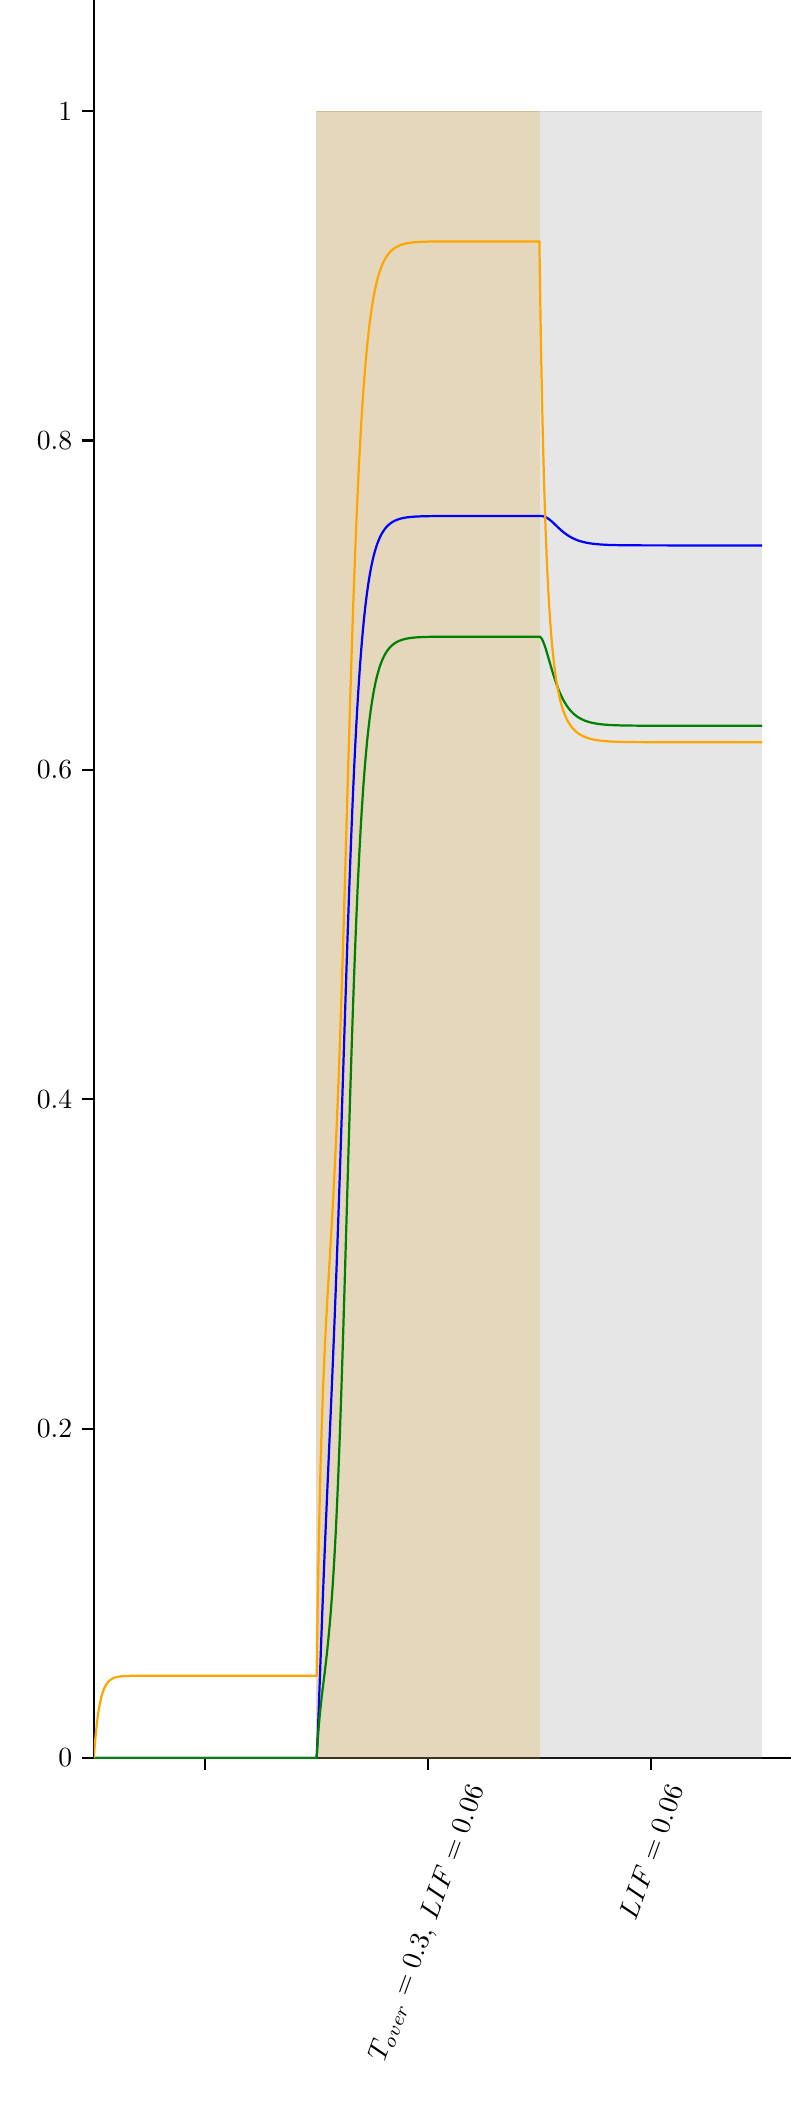
\begin{tikzpicture}[baseline]

\definecolor{darkgray176}{RGB}{176,176,176}
\definecolor{gray}{RGB}{128,128,128}
\definecolor{green}{RGB}{0,128,0}
\definecolor{lightgray204}{RGB}{204,204,204}
\definecolor{orange}{RGB}{255,165,0}

\begin{axis}[
 ytick={0,0.2,0.4,0.6,0.8,1},
 x tick label style = {rotate=70},
 y post scale=3, 
 transpose legend,
legend cell align={left},
legend style={
  fill opacity=0.8,
  draw opacity=1,
  text opacity=1,
  at={(axis cs:5,1.1)},
  anchor=south west,
    legend columns=4,
    /tikz/every even column/.append style={column sep=1.0cm},,
  draw=lightgray204
},
tick align=outside,
tick pos=left,
x grid style={darkgray176},
xmin=0, xmax=120,
xtick style={color=black},
xtick={20,60,100},
xticklabels={
  ,
  {\(\displaystyle T_\text{over}=0.3\), \(\displaystyle \text{LIF}=0.06\)},
  \(\displaystyle \text{LIF}=0.06\)
},
y grid style={darkgray176},
ymin=0, ymax=1.05,
ytick style={color=black}
]
\path [draw=orange, fill=orange, opacity=0.2]
(axis cs:40,0)
--(axis cs:40,1)
--(axis cs:80,1)
--(axis cs:80,0)
--cycle;

\path [draw=gray, fill=gray, opacity=0.2]
(axis cs:40,0)
--(axis cs:40,1)
--(axis cs:120,1)
--(axis cs:120,0)
--cycle;

\addplot [thick, blue]
table {%
0 0
0.0001 0
0.0011 0
0.0111 0
0.1111 0
0.2111 0
0.3111 0
0.4111 0
0.5111 0
0.6111 0
0.7111 0
0.8111 0
0.9111 0
1.0111 0
1.1111 0
1.2111 0
1.3111 0
1.4111 0
1.5111 0
1.6111 0
1.7111 0
1.8111 0
1.9111 0
2.0111 0
2.1111 0
2.2111 0
2.3111 0
2.4111 0
2.5111 0
2.6111 0
2.7111 0
2.8111 0
2.9111 0
3.0111 0
3.1111 0
3.2111 0
3.3111 0
3.4111 0
3.5111 0
3.6111 0
3.7111 0
3.8111 0
3.9111 0
4.0111 0
4.1111 0
4.2111 0
4.3111 0
4.4111 0
4.5111 0
4.6111 0
4.7111 0
4.8111 0
4.9111 0
5.0111 0
5.1111 0
5.2111 0
5.3111 0
5.4111 0
5.5111 0
5.6111 0
5.7111 0
5.8111 0
5.9111 0
6.0111 0
6.1111 0
6.21109999999999 0
6.31109999999999 0
6.41109999999999 0
6.51109999999999 0
6.61109999999999 0
6.71109999999999 0
6.81109999999999 0
6.91109999999999 0
7.01109999999999 0
7.11109999999999 0
7.21109999999999 0
7.31109999999999 0
7.41109999999999 0
7.51109999999999 0
7.61109999999999 0
7.71109999999999 0
7.81109999999999 0
7.91109999999999 0
8.01109999999999 0
8.11109999999999 0
8.21109999999999 0
8.31109999999999 0
8.41109999999999 0
8.51109999999999 0
8.61109999999999 0
8.71109999999999 0
8.81109999999999 0
8.91109999999999 0
9.01109999999998 0
9.11109999999998 0
9.21109999999998 0
9.31109999999998 0
9.41109999999998 0
9.51109999999998 0
9.61109999999998 0
9.71109999999998 0
9.81109999999998 0
9.91109999999998 0
10.0111 0
10.1111 0
10.2111 0
10.3111 0
10.4111 0
10.5111 0
10.6111 0
10.7111 0
10.8111 0
10.9111 0
11.0111 0
11.1111 0
11.2111 0
11.3111 0
11.4111 0
11.5111 0
11.6111 0
11.7111 0
11.8111 0
11.9111 0
12.0111 0
12.1111 0
12.2111 0
12.3111 0
12.4111 0
12.5111 0
12.6111 0
12.7111 0
12.8111 0
12.9111 0
13.0111 0
13.1111 0
13.2111 0
13.3111 0
13.4111 0
13.5111 0
13.6111 0
13.7111 0
13.8111 0
13.9111 0
14.0111 0
14.1111 0
14.2111 0
14.3111 0
14.4111 0
14.5111 0
14.6111 0
14.7111 0
14.8111 0
14.9111 0
15.0111 0
15.1111 0
15.2111 0
15.3111 0
15.4111 0
15.5111 0
15.6111 0
15.7111 0
15.8111 0
15.9111 0
16.0111 0
16.1111 0
16.2111 0
16.3111 0
16.4111 0
16.5111 0
16.6111 0
16.7111 0
16.8111 0
16.9111 0
17.0111 0
17.1111 0
17.2111 0
17.3111 0
17.4111 0
17.5111 0
17.6111 0
17.7111 0
17.8111 0
17.9111 0
18.0111 0
18.1111 0
18.2111 0
18.3111 0
18.4111 0
18.5111 0
18.6111 0
18.7111 0
18.8111 0
18.9111 0
19.0111 0
19.1111 0
19.2111 0
19.3111 0
19.4111 0
19.5111 0
19.6111 0
19.7111 0
19.8111 0
19.9111 0
20.0111 0
20.1111 0
20.2111 0
20.3111 0
20.4111 0
20.5111 0
20.6111 0
20.7111 0
20.8111 0
20.9111 0
21.0111 0
21.1111 0
21.2111 0
21.3111 0
21.4111 0
21.5111 0
21.6111 0
21.7111 0
21.8111 0
21.9111 0
22.0111 0
22.1111 0
22.2111 0
22.3111 0
22.4111000000001 0
22.5111000000001 0
22.6111000000001 0
22.7111000000001 0
22.8111000000001 0
22.9111000000001 0
23.0111000000001 0
23.1111000000001 0
23.2111000000001 0
23.3111000000001 0
23.4111000000001 0
23.5111000000001 0
23.6111000000001 0
23.7111000000001 0
23.8111000000001 0
23.9111000000001 0
24.0111000000001 0
24.1111000000001 0
24.2111000000001 0
24.3111000000001 0
24.4111000000001 0
24.5111000000001 0
24.6111000000001 0
24.7111000000001 0
24.8111000000001 0
24.9111000000001 0
25.0111000000001 0
25.1111000000001 0
25.2111000000001 0
25.3111000000001 0
25.4111000000001 0
25.5111000000001 0
25.6111000000001 0
25.7111000000001 0
25.8111000000001 0
25.9111000000001 0
26.0111000000001 0
26.1111000000001 0
26.2111000000001 0
26.3111000000001 0
26.4111000000001 0
26.5111000000001 0
26.6111000000001 0
26.7111000000001 0
26.8111000000001 0
26.9111000000001 0
27.0111000000001 0
27.1111000000001 0
27.2111000000001 0
27.3111000000001 0
27.4111000000001 0
27.5111000000001 0
27.6111000000001 0
27.7111000000001 0
27.8111000000001 0
27.9111000000001 0
28.0111000000001 0
28.1111000000001 0
28.2111000000001 0
28.3111000000001 0
28.4111000000001 0
28.5111000000001 0
28.6111000000001 0
28.7111000000001 0
28.8111000000001 0
28.9111000000001 0
29.0111000000001 0
29.1111000000001 0
29.2111000000001 0
29.3111000000001 0
29.4111000000002 0
29.5111000000002 0
29.6111000000002 0
29.7111000000002 0
29.8111000000002 0
29.9111000000002 0
30.0111000000002 0
30.1111000000002 0
30.2111000000002 0
30.3111000000002 0
30.4111000000002 0
30.5111000000002 0
30.6111000000002 0
30.7111000000002 0
30.8111000000002 0
30.9111000000002 0
31.0111000000002 0
31.1111000000002 0
31.2111000000002 0
31.3111000000002 0
31.4111000000002 0
31.5111000000002 0
31.6111000000002 0
31.7111000000002 0
31.8111000000002 0
31.9111000000002 0
32.0111000000002 0
32.1111000000002 0
32.2111000000002 0
32.3111000000002 0
32.4111000000002 0
32.5111000000002 0
32.6111000000002 0
32.7111000000002 0
32.8111000000002 0
32.9111000000002 0
33.0111000000002 0
33.1111000000002 0
33.2111000000002 0
33.3111000000002 0
33.4111000000002 0
33.5111000000002 0
33.6111000000002 0
33.7111000000002 0
33.8111000000002 0
33.9111000000002 0
34.0111000000002 0
34.1111000000002 0
34.2111000000002 0
34.3111000000002 0
34.4111000000002 0
34.5111000000002 0
34.6111000000002 0
34.7111000000002 0
34.8111000000002 0
34.9111000000002 0
35.0111000000002 0
35.1111000000002 0
35.2111000000002 0
35.3111000000002 0
35.4111000000002 0
35.5111000000002 0
35.6111000000002 0
35.7111000000002 0
35.8111000000002 0
35.9111000000002 0
36.0111000000002 0
36.1111000000002 0
36.2111000000002 0
36.3111000000002 0
36.4111000000002 0
36.5111000000002 0
36.6111000000002 0
36.7111000000003 0
36.8111000000003 0
36.9111000000003 0
37.0111000000003 0
37.1111000000003 0
37.2111000000003 0
37.3111000000003 0
37.4111000000003 0
37.5111000000003 0
37.6111000000003 0
37.7111000000003 0
37.8111000000003 0
37.9111000000003 0
38.0111000000003 0
38.1111000000003 0
38.2111000000003 0
38.3111000000003 0
38.4111000000003 0
38.5111000000003 0
38.6111000000003 0
38.7111000000003 0
38.8111000000003 0
38.9111000000003 0
39.0111000000003 0
39.1111000000003 0
39.2111000000003 0
39.3111000000003 0
39.4111000000003 0
39.5111000000003 0
39.6111000000003 0
39.7111000000003 0
39.8111000000003 0
39.9111000000003 0
40 0
40 0
40.0115348003323 0.00070129486902565
40.1115348003323 0.0074713537807524
40.2115348003323 0.0152313305944161
40.3115348003323 0.0236846089484518
40.4115348003323 0.0325951158909974
40.5115348003323 0.0417774747941581
40.6115348003323 0.051088832552304
40.7115348003323 0.0604218236441233
40.8115348003323 0.0696984059774012
40.9115348003323 0.0788644534789488
41.0115348003323 0.0878850562156867
41.1115348003323 0.0967404956141112
41.2115348003323 0.105422856142046
41.3115348003323 0.11393322198154
41.4115348003323 0.122279396249071
41.5115348003323 0.130474074398911
41.6115348003323 0.138533402766155
41.7115348003323 0.146475856616248
41.8115348003323 0.154321378080348
41.9115348003323 0.162090721645049
42.0115348003323 0.169804962445913
42.1115348003323 0.177485129850553
42.2115348003323 0.185151935357833
42.3115348003323 0.192825569539665
42.4115348003323 0.200525547599228
42.5115348003323 0.208270587181702
42.6115348003323 0.21607850545859
42.7115348003323 0.223966125338304
42.8115348003323 0.231949183057705
42.9115348003323 0.240042231496859
43.0115348003323 0.248258535432186
43.1115348003323 0.256609956682551
43.2115348003323 0.265106828766707
43.3115348003323 0.273757822311135
43.4115348003323 0.282569804027974
43.5115348003323 0.291547693595709
43.6115348003324 0.300694324162289
43.7115348003324 0.310010313365565
43.8115348003324 0.319493952623955
43.9115348003324 0.329141122878089
44.0115348003324 0.338945244858511
44.1115348003324 0.348897271240656
44.2115348003324 0.358985726699871
44.3115348003324 0.369196799933093
44.4115348003324 0.379514489277374
44.5115348003324 0.389920800803011
44.6115348003324 0.40039599491548
44.7115348003324 0.410918874815232
44.8115348003324 0.421467107879009
44.9115348003324 0.432017569341321
45.0115348003324 0.442546696703517
45.1115348003324 0.453030843131279
45.2115348003324 0.46344661868592
45.3115348003324 0.473771209463897
45.4115348003324 0.483982666433386
45.5115348003324 0.494060157770807
45.6115348003324 0.503984180626481
45.7115348003324 0.513736730319688
45.8115348003324 0.52330142684573
45.9115348003324 0.532663600178914
46.0115348003324 0.541810337124624
46.1115348003324 0.550730493396908
46.2115348003324 0.559414675190261
46.3115348003324 0.567855194811183
46.4115348003324 0.576046004984307
46.5115348003324 0.583982616301743
46.6115348003324 0.591662001994656
46.7115348003324 0.59908249382016
46.8115348003324 0.606243672415011
46.9115348003324 0.613146255003283
47.0115348003324 0.619791982883704
47.1115348003324 0.626183510681832
47.2115348003324 0.63232429894536
47.3115348003324 0.638218511294653
47.4115348003324 0.643870917018793
47.5115348003324 0.649286799730402
47.6115348003324 0.654471872458751
47.7115348003324 0.659432199367356
47.8115348003324 0.664174124125583
47.9115348003324 0.668704204839691
48.0115348003324 0.673029155353013
48.1115348003324 0.677155792653535
48.2115348003324 0.68109099007612
48.3115348003324 0.684841635952614
48.4115348003324 0.688414597342924
48.5115348003324 0.691816688471101
48.6115348003324 0.695054643490224
48.7115348003324 0.698135093206435
48.8115348003324 0.701064545404059
48.9115348003324 0.703849368429139
49.0115348003324 0.706495777706579
49.1115348003324 0.709009824885648
49.2115348003324 0.711397389329028
49.3115348003324 0.71366417168139
49.4115348003324 0.715815689274068
49.5115348003324 0.717857273142608
49.6115348003324 0.71979406645342
49.7115348003324 0.721631024154298
49.8115348003324 0.723372913681145
49.9115348003324 0.725024316569702
50.0115348003324 0.726589630836425
50.1115348003324 0.728073074006877
50.2115348003324 0.729478686683147
50.3115348003324 0.730810336553823
50.4115348003324 0.732071722761081
50.5115348003324 0.733266380549478
50.6115348003324 0.734397686130136
50.7115348003325 0.735468861702265
50.8115348003325 0.736482980581378
50.9115348003325 0.737442972390271
51.0115348003325 0.738351628274814
51.1115348003325 0.739211606111978
51.2115348003325 0.740025435682317
51.3115348003325 0.740795523783369
51.4115348003325 0.741524159264239
51.5115348003325 0.742213517964966
51.6115348003325 0.742865667547233
51.7115348003325 0.743482572205577
51.8115348003325 0.744066097250548
51.9115348003325 0.744618013557235
52.0115348003325 0.745140001874358
52.1115348003325 0.745633656990583
52.2115348003325 0.746100491756068
52.3115348003325 0.746541940958335
52.4115348003325 0.746959365052543
52.5115348003325 0.747354053747042
52.6115348003325 0.747727229445793
52.7115348003325 0.748080050549781
52.8115348003325 0.748413614620071
52.9115348003325 0.748728961405517
53.0115348003325 0.749027075738447
53.1115348003325 0.749308890301923
53.2115348003325 0.749575288272327
53.3115348003325 0.749827105841201
53.4115348003325 0.75006513462033
53.5115348003325 0.750290123934146
53.6115348003325 0.750502783003536
53.7115348003325 0.750703783025139
53.8115348003325 0.750893759150215
53.9115348003325 0.751073312367074
54.0115348003325 0.751243011291065
54.1115348003325 0.751403393865965
54.2115348003325 0.751554968980611
54.3115348003325 0.751698218004445
54.4115348003325 0.751833596245606
54.5115348003325 0.751961534335034
54.6115348003325 0.752082439540014
54.7115348003325 0.752196697010396
54.8115348003325 0.752304670960673
54.9115348003325 0.752406705790961
55.0115348003325 0.752503127149799
55.1115348003325 0.752594242941599
55.2115348003325 0.752680344281428
55.3115348003325 0.75276170639974
55.4115348003325 0.752838589499514
55.5115348003325 0.752911239568182
55.6115348003325 0.752979889146622
55.7115348003325 0.753044758057384
55.8115348003325 0.753106054094205
55.9115348003325 0.753163973674817
56.0115348003325 0.753218702458899
56.1115348003325 0.753270415932996
56.2115348003325 0.753319279964104
56.3115348003325 0.753365451323536
56.4115348003325 0.753409078182647
56.5115348003325 0.753450300581861
56.6115348003325 0.753489250874421
56.7115348003325 0.753526054146179
56.8115348003325 0.753560828612703
56.9115348003325 0.75359368599489
57.0115348003325 0.753624731874236
57.1115348003325 0.753654066028833
57.2115348003325 0.753681782751132
57.3115348003325 0.753707971148439
57.4115348003325 0.753732715427062
57.5115348003325 0.753756095161006
57.6115348003325 0.753778185546015
57.7115348003326 0.753799057639781
57.8115348003326 0.753818778589038
57.9115348003326 0.753837411844269
58.0115348003326 0.753855017362678
58.1115348003326 0.753871651800074
58.2115348003326 0.753887368692262
58.3115348003326 0.753902218626509
58.4115348003326 0.753916249403625
58.5115348003326 0.753929506191168
58.6115348003326 0.753942031668257
58.7115348003326 0.753953866162445
58.8115348003326 0.753965047779091
58.9115348003326 0.753975612523635
59.0115348003326 0.753985594417158
59.1115348003326 0.753995025605612
59.2115348003326 0.754003936463041
59.3115348003326 0.754012355689139
59.4115348003326 0.754020310401449
59.5115348003326 0.75402782622249
59.6115348003326 0.754034927362107
59.7115348003326 0.75404163669528
59.8115348003326 0.754047975835666
59.9115348003326 0.75405396520509
60.0115348003326 0.754059624099214
60.1115348003326 0.754064970749597
60.2115348003326 0.754070022382337
60.3115348003326 0.754074795273483
60.4115348003326 0.754079304801405
60.5115348003326 0.754083565496269
60.6115348003326 0.754087591086801
60.7115348003326 0.754091394544467
60.8115348003326 0.754094988125221
60.9115348003326 0.754098383408957
61.0115348003326 0.754101591336785
61.1115348003326 0.754104622246252
61.2115348003326 0.754107485904628
61.3115348003326 0.754110191540354
61.4115348003326 0.754112747872752
61.5115348003326 0.754115163140111
61.6115348003326 0.754117445126211
61.7115348003326 0.754119601185394
61.8115348003326 0.754121638266249
61.9115348003326 0.754123562933992
62.0115348003326 0.754125381391613
62.1115348003326 0.754127099499859
62.2115348003326 0.75412872279611
62.3115348003326 0.754130256512215
62.4115348003326 0.754131705591354
62.5115348003326 0.754133074703955
62.6115348003326 0.754134368262746
62.7115348003326 0.754135590436969
62.8115348003326 0.754136745165815
62.9115348003326 0.754137836171114
63.0115348003326 0.75413886696933
63.1115348003326 0.754139840882889
63.2115348003326 0.754140761050884
63.3115348003326 0.754141630439192
63.4115348003326 0.754142451850033
63.5115348003326 0.754143227930994
63.6115348003326 0.754143961183566
63.7115348003326 0.754144653971203
63.8115348003326 0.75414530852694
63.9115348003326 0.754145926960587
64.0115348003326 0.75414651126553
64.1115348003326 0.754147063325153
64.2115348003326 0.754147584918912
64.3115348003326 0.754148077728064
64.4115348003326 0.754148543341091
64.5115348003326 0.754148983258816
64.6115348003326 0.754149398899241
64.7115348003326 0.754149791602116
64.8115348003326 0.75415016263326
64.9115348003326 0.754150513188638
65.0115348003326 0.754150844398217
65.1115348003326 0.754151157329606
65.2115348003326 0.7541514529915
65.3115348003326 0.754151732336928
65.4115348003326 0.754151996266328
65.5115348003326 0.754152245630446
65.6115348003325 0.75415248123308
65.7115348003325 0.75415270383367
65.8115348003325 0.754152914149747
65.9115348003325 0.754153112859244
66.0115348003325 0.754153300602683
66.1115348003325 0.754153477985236
66.2115348003325 0.754153645578683
66.3115348003325 0.754153803923244
66.4115348003325 0.754153953529333
66.5115348003325 0.75415409487919
66.6115348003325 0.754154228428447
66.7115348003325 0.754154354607591
66.8115348003325 0.754154473823349
66.9115348003325 0.754154586460005
67.0115348003325 0.754154692880637
67.1115348003325 0.754154793428283
67.2115348003325 0.754154888427053
67.3115348003325 0.754154978183169
67.4115348003324 0.754155062985955
67.5115348003324 0.754155143108766
67.6115348003324 0.754155218809874
67.7115348003324 0.754155290333297
67.8115348003324 0.754155357909586
67.9115348003324 0.754155421756571
68.0115348003324 0.754155482080058
68.1115348003324 0.754155539074497
68.2115348003324 0.754155592923606
68.3115348003324 0.754155643800966
68.4115348003324 0.754155691870576
68.5115348003324 0.754155737287387
68.6115348003324 0.754155780197797
68.7115348003324 0.754155820740127
68.8115348003324 0.754155859045062
68.9115348003324 0.754155895236077
69.0115348003324 0.754155929429831
69.1115348003324 0.754155961736547
69.2115348003323 0.754155992260363
69.3115348003323 0.754156021099673
69.4115348003323 0.754156048347438
69.5115348003323 0.754156074091489
69.6115348003323 0.754156098414813
69.7115348003323 0.754156121395814
69.8115348003323 0.75415614310857
69.9115348003323 0.754156163623072
70.0115348003323 0.754156183005447
70.1115348003323 0.754156201318173
70.2115348003323 0.754156218620281
70.3115348003323 0.754156234967543
70.4115348003323 0.754156250412655
70.5115348003323 0.754156265005402
70.6115348003323 0.754156278792824
70.7115348003323 0.754156291819364
70.8115348003323 0.754156304127013
70.9115348003322 0.754156315755443
71.0115348003322 0.754156326742139
71.1115348003322 0.754156337122516
71.2115348003322 0.754156346930034
71.3115348003322 0.754156356196308
71.4115348003322 0.754156364951207
71.5115348003322 0.754156373222952
71.6115348003322 0.754156381038208
71.7115348003322 0.754156388422165
71.8115348003322 0.754156395398626
71.9115348003322 0.754156401990079
72.0115348003322 0.754156408217772
72.1115348003322 0.754156414101779
72.2115348003322 0.754156419661067
72.3115348003322 0.754156424913557
72.4115348003322 0.754156429876179
72.5115348003322 0.75415643456493
72.6115348003322 0.754156438994925
72.7115348003321 0.754156443180443
72.8115348003321 0.754156447134976
72.9115348003321 0.754156450871272
73.0115348003321 0.754156454401374
73.1115348003321 0.754156457736661
73.2115348003321 0.754156460887885
73.3115348003321 0.754156463865203
73.4115348003321 0.754156466678213
73.5115348003321 0.754156469335982
73.6115348003321 0.754156471847077
73.7115348003321 0.754156474219594
73.8115348003321 0.754156476461179
73.9115348003321 0.754156478579059
74.0115348003321 0.75415648058006
74.1115348003321 0.754156482470632
74.2115348003321 0.75415648425687
74.3115348003321 0.754156485944531
74.411534800332 0.754156487539056
74.511534800332 0.754156489045584
74.611534800332 0.754156490468972
74.711534800332 0.754156491813808
74.811534800332 0.754156493084427
74.911534800332 0.754156494284924
75.011534800332 0.75415649541917
75.111534800332 0.754156496490821
75.211534800332 0.754156497503331
75.311534800332 0.754156498459964
75.411534800332 0.754156499363803
75.511534800332 0.754156500217763
75.611534800332 0.754156501024595
75.711534800332 0.754156501786901
75.811534800332 0.754156502507138
75.911534800332 0.754156503187627
76.011534800332 0.754156503830563
76.111534800332 0.754156504438017
76.2115348003319 0.754156505011947
76.3115348003319 0.754156505554204
76.4115348003319 0.754156506066536
76.5115348003319 0.754156506550594
76.6115348003319 0.754156507007938
76.7115348003319 0.754156507440043
76.8115348003319 0.754156507848302
76.9115348003319 0.75415650823403
77.0115348003319 0.754156508598471
77.1115348003319 0.7541565089428
77.2115348003319 0.754156509268126
77.3115348003319 0.754156509575499
77.4115348003319 0.754156509865909
77.5115348003319 0.754156510140292
77.6115348003319 0.754156510399533
77.7115348003319 0.754156510644467
77.8115348003319 0.754156510875884
77.9115348003319 0.75415651109453
78.0115348003318 0.754156511301109
78.1115348003318 0.754156511496289
78.2115348003318 0.754156511680696
78.3115348003318 0.754156511854927
78.4115348003318 0.754156512019543
78.5115348003318 0.754156512175074
78.6115348003318 0.754156512322022
78.7115348003318 0.754156512460861
78.8115348003318 0.754156512592037
78.9115348003318 0.754156512715974
79.0115348003318 0.754156512833071
79.1115348003318 0.754156512943707
79.2115348003318 0.754156513048236
79.3115348003318 0.754156513146997
79.4115348003318 0.754156513240308
79.5115348003318 0.754156513328469
79.6115348003318 0.754156513411765
79.7115348003317 0.754156513490464
79.8115348003317 0.75415651356482
79.9115348003317 0.754156513635072
80 0.754156513693982
80 0.754156513693982
80.1 0.754155725774723
80.2 0.754150481871002
80.3 0.754137036589557
80.4 0.754112347702299
80.5 0.754074002406912
80.6 0.754020148968961
80.7 0.753949433247177
80.8 0.75386093974731
80.8999999999999 0.753754136950818
80.9999999999999 0.753628826730519
81.0999999999999 0.753485097703928
81.1999999999999 0.753323282393452
81.2999999999999 0.753143918067189
81.3999999999999 0.752947711129702
81.4999999999999 0.752735504922897
81.5999999999999 0.752508250785751
81.6999999999999 0.752266982210378
81.7999999999999 0.752012791921945
81.8999999999999 0.751746811702201
81.9999999999999 0.751470194771202
82.0999999999999 0.751184100539274
82.1999999999999 0.750889681541362
82.2999999999999 0.750588072368299
82.3999999999999 0.750280380414016
82.4999999999999 0.749967678263889
82.5999999999999 0.74965099755702
82.6999999999998 0.749331324163806
82.7999999999998 0.74900959452958
82.8999999999998 0.748686693044925
82.9999999999998 0.748363450313353
83.0999999999998 0.748040642197201
83.1999999999998 0.747718989532626
83.2999999999998 0.747399158414333
83.3999999999998 0.747081760960132
83.4999999999998 0.746767356474394
83.5999999999998 0.74645645293798
83.6999999999998 0.746149508760227
83.7999999999998 0.745846934735988
83.8999999999998 0.745549096157618
83.9999999999998 0.745256315038139
84.0999999999998 0.7449688724076
84.1999999999998 0.744687010649932
84.2999999999998 0.744410935852338
84.3999999999997 0.74414082014361
84.4999999999997 0.743876804001536
84.5999999999997 0.743618998513065
84.6999999999997 0.743367487573885
84.7999999999997 0.74312233001678
84.8999999999997 0.742883561660484
84.9999999999997 0.742651197272799
85.0999999999997 0.742425232443541
85.1999999999997 0.742205645364399
85.2999999999997 0.741992398514125
85.3999999999997 0.741785440248577
85.4999999999997 0.741584706296094
85.5999999999997 0.74139012115944
85.6999999999997 0.741201599426226
85.7999999999997 0.741019046990222
85.8999999999997 0.74084236218639
85.9999999999997 0.740671436842787
86.0999999999997 0.740506157252732
86.1999999999996 0.740346405070795
86.2999999999996 0.740192058136274
86.3999999999996 0.740042991227883
86.4999999999996 0.739899076753397
86.5999999999996 0.739760185377963
86.6999999999996 0.739626186594751
86.7999999999996 0.739496949241529
86.8999999999996 0.739372341966659
86.9999999999996 0.739252233647891
87.0999999999996 0.739136493767224
87.1999999999996 0.739024992744947
87.2999999999996 0.738917602235866
87.3999999999996 0.738814195390544
87.4999999999996 0.738714647084275
87.5999999999996 0.738618834116329
87.6999999999996 0.738526635381914
87.7999999999996 0.73843793201909
87.8999999999996 0.738352607532805
87.9999999999995 0.738270547898032
88.0999999999995 0.738191641643896
88.1999999999995 0.73811577992052
88.2999999999995 0.738042856550233
88.3999999999995 0.737972768064641
88.4999999999995 0.737905413728969
88.5999999999995 0.73784069555498
88.6999999999995 0.737778518303652
88.7999999999995 0.737718789478747
88.8999999999995 0.737661419312278
88.9999999999995 0.737606320742811
89.0999999999995 0.737553409387477
89.1999999999995 0.737502603508476
89.2999999999995 0.73745382397479
89.3999999999995 0.737406994219782
89.4999999999995 0.737362040195263
89.5999999999995 0.737318890322586
89.6999999999994 0.737277475441265
89.7999999999994 0.737237728755559
89.8999999999994 0.737199585779432
89.9999999999994 0.737162984280264
90.0999999999994 0.737127864221627
90.1999999999994 0.737094167705433
90.2999999999994 0.737061838913718
90.3999999999994 0.737030824050289
90.4999999999994 0.737001071282454
90.5999999999994 0.736972530683016
90.6999999999994 0.736945154172689
90.7999999999994 0.736918895463088
90.8999999999994 0.736893710000417
90.9999999999994 0.736869554909948
91.0999999999994 0.736846388941412
91.1999999999994 0.736824172415348
91.2999999999994 0.73680286717051
91.3999999999994 0.736782436512357
91.4999999999993 0.736762845162692
91.5999999999993 0.736744059210477
91.6999999999993 0.736726046063858
91.7999999999993 0.736708774403406
91.8999999999993 0.736692214136611
91.9999999999993 0.736676336353616
92.0999999999993 0.736661113284201
92.1999999999993 0.736646518256023
92.2999999999993 0.736632525654092
92.3999999999993 0.736619110881487
92.4999999999993 0.736606250321287
92.5999999999993 0.736593921299709
92.6999999999993 0.736582102050442
92.7999999999993 0.73657077168014
92.8999999999993 0.736559910135062
92.9999999999993 0.736549498168849
93.0999999999993 0.736539517311386
93.1999999999992 0.736529949838749
93.2999999999992 0.736520778744202
93.3999999999992 0.736511987710212
93.4999999999992 0.73650356108147
93.5999999999992 0.736495483838876
93.6999999999992 0.736487741574469
93.7999999999992 0.736480320467276
93.8999999999992 0.736473207260048
93.9999999999992 0.736466389236862
94.0999999999992 0.736459854201554
94.1999999999992 0.736453590456969
94.2999999999992 0.736447586784985
94.3999999999992 0.73644183242731
94.4999999999992 0.736436317066998
94.5999999999992 0.736431030810682
94.6999999999992 0.736425964171489
94.7999999999992 0.736421108052621
94.8999999999992 0.736416453731562
94.9999999999991 0.736411992844917
95.0999999999991 0.73640771737383
95.1999999999991 0.736403619629986
95.2999999999991 0.736399692242154
95.3999999999991 0.736395928143273
95.4999999999991 0.736392320558038
95.5999999999991 0.736388862990992
95.6999999999991 0.736385549215079
95.7999999999991 0.736382373260664
95.8999999999991 0.736379329404991
95.9999999999991 0.736376412162057
96.0999999999991 0.736373616272903
96.1999999999991 0.736370936696286
96.2999999999991 0.736368368599738
96.3999999999991 0.736365907350975
96.4999999999991 0.736363548509662
96.5999999999991 0.736361287819509
96.6999999999991 0.736359121200686
96.799999999999 0.73635704474255
96.899999999999 0.736355054696668
96.999999999999 0.736353147470117
97.099999999999 0.736351319619068
97.199999999999 0.736349567842625
97.299999999999 0.736347888976918
97.399999999999 0.736346279989439
97.499999999999 0.736344737973607
97.599999999999 0.736343260143557
97.699999999999 0.736341843829148
97.799999999999 0.736340486471166
97.899999999999 0.736339185616732
97.999999999999 0.736337938914898
98.099999999999 0.736336744112421
98.199999999999 0.736335599049711
98.299999999999 0.736334501656954
98.399999999999 0.736333449950382
98.4999999999989 0.736332442028706
98.5999999999989 0.736331476069696
98.6999999999989 0.736330550326898
98.7999999999989 0.736329663126488
98.8999999999989 0.736328812864259
98.9999999999989 0.736327998002727
99.0999999999989 0.736327217068365
99.1999999999989 0.73632646864894
99.2999999999989 0.736325751390975
99.3999999999989 0.736325063997298
99.4999999999989 0.736324405224711
99.5999999999989 0.736323773881743
99.6999999999989 0.736323168826501
99.7999999999989 0.736322588964607
99.8999999999989 0.736322033247225
99.9999999999989 0.736321500669169
100.099999999999 0.736320990267085
100.199999999999 0.736320501117713
100.299999999999 0.736320032336217
100.399999999999 0.736319583074593
100.499999999999 0.736319152520131
100.599999999999 0.736318739893949
100.699999999999 0.736318344449588
100.799999999999 0.73631796547166
100.899999999999 0.736317602274556
100.999999999999 0.736317254201209
101.099999999999 0.736316920621903
101.199999999999 0.73631660093314
101.299999999999 0.736316294556543
101.399999999999 0.736316000937815
101.499999999999 0.736315719545736
101.599999999999 0.736315449871201
101.699999999999 0.736315191426301
101.799999999999 0.736314943743441
101.899999999999 0.736314706374493
101.999999999999 0.73631447888999
102.099999999999 0.736314260878341
102.199999999999 0.736314051945095
102.299999999999 0.736313851712226
102.399999999999 0.736313659817444
102.499999999999 0.736313475913546
102.599999999999 0.736313299667785
102.699999999999 0.736313130761269
102.799999999999 0.736312968888385
102.899999999999 0.736312813756244
102.999999999999 0.736312665084152
103.099999999999 0.736312522603104
103.199999999999 0.736312386055297
103.299999999999 0.73631225519366
103.399999999999 0.736312129781413
103.499999999999 0.736312009591633
103.599999999999 0.736311894406847
103.699999999999 0.736311784018638
103.799999999999 0.736311678227268
103.899999999999 0.736311576841315
103.999999999999 0.736311479677328
104.099999999999 0.736311386559496
104.199999999999 0.736311297319328
104.299999999999 0.73631121179535
104.399999999999 0.736311129832812
104.499999999999 0.736311051283406
104.599999999999 0.736310976005003
104.699999999999 0.736310903861391
104.799999999999 0.736310834722028
104.899999999999 0.736310768461811
104.999999999999 0.736310704960845
105.099999999999 0.736310644104229
105.199999999999 0.736310585781844
105.299999999999 0.73631052988816
105.399999999999 0.736310476322039
105.499999999999 0.736310424986555
105.599999999999 0.736310375788819
105.699999999999 0.73631032863981
105.799999999999 0.736310283454213
105.899999999999 0.736310240150266
105.999999999999 0.736310198649614
106.099999999999 0.736310158877161
106.199999999999 0.736310120760942
106.299999999999 0.736310084231986
106.399999999998 0.736310049224195
106.499999999998 0.736310015674224
106.599999999998 0.736309983521365
106.699999999998 0.73630995270744
106.799999999998 0.73630992317669
106.899999999998 0.736309894875682
106.999999999998 0.736309867753205
107.099999999998 0.736309841760183
107.199999999998 0.736309816849581
107.299999999998 0.736309792976325
107.399999999998 0.736309770097216
107.499999999998 0.736309748170857
107.599999999998 0.736309727157571
107.699999999998 0.736309707019336
107.799999999998 0.736309687719713
107.899999999998 0.736309669223778
107.999999999998 0.736309651498065
108.099999999998 0.7363096345105
108.199999999998 0.736309618230343
108.299999999998 0.736309602628137
108.399999999998 0.736309587675649
108.499999999998 0.736309573345824
108.599999999998 0.736309559612732
108.699999999998 0.736309546451524
108.799999999998 0.736309533838385
108.899999999998 0.736309521750491
108.999999999998 0.736309510165971
109.099999999998 0.736309499063861
109.199999999998 0.736309488424074
109.299999999998 0.736309478227357
109.399999999998 0.736309468455259
109.499999999998 0.736309459090098
109.599999999998 0.736309450114928
109.699999999998 0.736309441513508
109.799999999998 0.736309433270276
109.899999999998 0.736309425370314
109.999999999998 0.736309417799328
110.099999999998 0.736309410543618
110.199999999998 0.736309403590057
110.299999999998 0.73630939692606
110.399999999998 0.736309390539571
110.499999999998 0.736309384419033
110.599999999998 0.73630937855337
110.699999999998 0.73630937293197
110.799999999998 0.73630936754466
110.899999999998 0.736309362381693
110.999999999998 0.736309357433725
111.099999999998 0.736309352691805
111.199999999998 0.736309348147351
111.299999999998 0.73630934379214
111.399999999998 0.736309339618293
111.499999999998 0.736309335618256
111.599999999998 0.736309331784791
111.699999999998 0.736309328110962
111.799999999998 0.736309324590122
111.899999999998 0.736309321215899
111.999999999998 0.736309317982187
112.099999999998 0.736309314883137
112.199999999998 0.736309311913139
112.299999999998 0.73630930906682
112.399999999998 0.73630930633903
112.499999999998 0.736309303724832
112.599999999998 0.736309301219496
112.699999999998 0.73630929881849
112.799999999998 0.736309296517468
112.899999999998 0.736309294312267
112.999999999998 0.736309292198896
113.099999999998 0.736309290173532
113.199999999998 0.73630928823251
113.299999999998 0.736309286372317
113.399999999998 0.736309284589587
113.499999999998 0.736309282881096
113.599999999998 0.73630928124375
113.699999999998 0.736309279674588
113.799999999998 0.73630927817077
113.899999999998 0.736309276729576
113.999999999998 0.736309275348396
114.099999999998 0.736309274024733
114.199999999998 0.736309272756191
114.299999999998 0.736309271540474
114.399999999998 0.736309270375383
114.499999999998 0.736309269258809
114.599999999998 0.736309268188733
114.699999999998 0.736309267163217
114.799999999998 0.736309266180407
114.899999999998 0.736309265238524
114.999999999998 0.736309264335863
115.099999999998 0.736309263470792
115.199999999998 0.736309262641744
115.299999999998 0.73630926184722
115.399999999998 0.736309261085783
115.499999999998 0.736309260356053
115.599999999998 0.736309259656712
115.699999999998 0.736309258986493
115.799999999998 0.736309258344184
115.899999999998 0.736309257728623
115.999999999998 0.736309257138695
116.099999999998 0.736309256573333
116.199999999998 0.736309256031514
116.299999999998 0.736309255512258
116.399999999998 0.736309255014626
116.499999999998 0.736309254537716
116.599999999998 0.736309254080666
116.699999999998 0.736309253642649
116.799999999998 0.736309253222872
116.899999999998 0.736309252820576
116.999999999998 0.736309252435032
117.099999999998 0.736309252065544
117.199999999998 0.736309251711442
117.299999999998 0.736309251372086
117.399999999998 0.736309251046861
117.499999999998 0.73630925073518
117.599999999998 0.736309250436478
117.699999999998 0.736309250150215
117.799999999998 0.736309249875872
117.899999999998 0.736309249612954
117.999999999998 0.736309249360985
118.099999999998 0.736309249119508
118.199999999998 0.736309248888087
118.299999999998 0.736309248666303
118.399999999998 0.736309248453754
118.499999999998 0.736309248250057
118.599999999998 0.736309248054842
118.699999999998 0.736309247867757
118.799999999998 0.736309247688462
118.899999999998 0.736309247516634
118.999999999998 0.736309247351961
119.099999999998 0.736309247194145
119.199999999998 0.736309247042902
119.299999999998 0.736309246897956
119.399999999998 0.736309246759047
119.499999999998 0.736309246625922
119.599999999998 0.73630924649834
119.699999999998 0.736309246376072
119.799999999998 0.736309246258895
119.899999999998 0.736309246146598
119.999999999998 0.736309246038977
120 0.736309246038977
};
\addplot [thick, green]
table {%
0 0
0.0001 0
0.0011 0
0.0111 0
0.1111 0
0.2111 0
0.3111 0
0.4111 0
0.5111 0
0.6111 0
0.7111 0
0.8111 0
0.9111 0
1.0111 0
1.1111 0
1.2111 0
1.3111 0
1.4111 0
1.5111 0
1.6111 0
1.7111 0
1.8111 0
1.9111 0
2.0111 0
2.1111 0
2.2111 0
2.3111 0
2.4111 0
2.5111 0
2.6111 0
2.7111 0
2.8111 0
2.9111 0
3.0111 0
3.1111 0
3.2111 0
3.3111 0
3.4111 0
3.5111 0
3.6111 0
3.7111 0
3.8111 0
3.9111 0
4.0111 0
4.1111 0
4.2111 0
4.3111 0
4.4111 0
4.5111 0
4.6111 0
4.7111 0
4.8111 0
4.9111 0
5.0111 0
5.1111 0
5.2111 0
5.3111 0
5.4111 0
5.5111 0
5.6111 0
5.7111 0
5.8111 0
5.9111 0
6.0111 0
6.1111 0
6.21109999999999 0
6.31109999999999 0
6.41109999999999 0
6.51109999999999 0
6.61109999999999 0
6.71109999999999 0
6.81109999999999 0
6.91109999999999 0
7.01109999999999 0
7.11109999999999 0
7.21109999999999 0
7.31109999999999 0
7.41109999999999 0
7.51109999999999 0
7.61109999999999 0
7.71109999999999 0
7.81109999999999 0
7.91109999999999 0
8.01109999999999 0
8.11109999999999 0
8.21109999999999 0
8.31109999999999 0
8.41109999999999 0
8.51109999999999 0
8.61109999999999 0
8.71109999999999 0
8.81109999999999 0
8.91109999999999 0
9.01109999999998 0
9.11109999999998 0
9.21109999999998 0
9.31109999999998 0
9.41109999999998 0
9.51109999999998 0
9.61109999999998 0
9.71109999999998 0
9.81109999999998 0
9.91109999999998 0
10.0111 0
10.1111 0
10.2111 0
10.3111 0
10.4111 0
10.5111 0
10.6111 0
10.7111 0
10.8111 0
10.9111 0
11.0111 0
11.1111 0
11.2111 0
11.3111 0
11.4111 0
11.5111 0
11.6111 0
11.7111 0
11.8111 0
11.9111 0
12.0111 0
12.1111 0
12.2111 0
12.3111 0
12.4111 0
12.5111 0
12.6111 0
12.7111 0
12.8111 0
12.9111 0
13.0111 0
13.1111 0
13.2111 0
13.3111 0
13.4111 0
13.5111 0
13.6111 0
13.7111 0
13.8111 0
13.9111 0
14.0111 0
14.1111 0
14.2111 0
14.3111 0
14.4111 0
14.5111 0
14.6111 0
14.7111 0
14.8111 0
14.9111 0
15.0111 0
15.1111 0
15.2111 0
15.3111 0
15.4111 0
15.5111 0
15.6111 0
15.7111 0
15.8111 0
15.9111 0
16.0111 0
16.1111 0
16.2111 0
16.3111 0
16.4111 0
16.5111 0
16.6111 0
16.7111 0
16.8111 0
16.9111 0
17.0111 0
17.1111 0
17.2111 0
17.3111 0
17.4111 0
17.5111 0
17.6111 0
17.7111 0
17.8111 0
17.9111 0
18.0111 0
18.1111 0
18.2111 0
18.3111 0
18.4111 0
18.5111 0
18.6111 0
18.7111 0
18.8111 0
18.9111 0
19.0111 0
19.1111 0
19.2111 0
19.3111 0
19.4111 0
19.5111 0
19.6111 0
19.7111 0
19.8111 0
19.9111 0
20.0111 0
20.1111 0
20.2111 0
20.3111 0
20.4111 0
20.5111 0
20.6111 0
20.7111 0
20.8111 0
20.9111 0
21.0111 0
21.1111 0
21.2111 0
21.3111 0
21.4111 0
21.5111 0
21.6111 0
21.7111 0
21.8111 0
21.9111 0
22.0111 0
22.1111 0
22.2111 0
22.3111 0
22.4111000000001 0
22.5111000000001 0
22.6111000000001 0
22.7111000000001 0
22.8111000000001 0
22.9111000000001 0
23.0111000000001 0
23.1111000000001 0
23.2111000000001 0
23.3111000000001 0
23.4111000000001 0
23.5111000000001 0
23.6111000000001 0
23.7111000000001 0
23.8111000000001 0
23.9111000000001 0
24.0111000000001 0
24.1111000000001 0
24.2111000000001 0
24.3111000000001 0
24.4111000000001 0
24.5111000000001 0
24.6111000000001 0
24.7111000000001 0
24.8111000000001 0
24.9111000000001 0
25.0111000000001 0
25.1111000000001 0
25.2111000000001 0
25.3111000000001 0
25.4111000000001 0
25.5111000000001 0
25.6111000000001 0
25.7111000000001 0
25.8111000000001 0
25.9111000000001 0
26.0111000000001 0
26.1111000000001 0
26.2111000000001 0
26.3111000000001 0
26.4111000000001 0
26.5111000000001 0
26.6111000000001 0
26.7111000000001 0
26.8111000000001 0
26.9111000000001 0
27.0111000000001 0
27.1111000000001 0
27.2111000000001 0
27.3111000000001 0
27.4111000000001 0
27.5111000000001 0
27.6111000000001 0
27.7111000000001 0
27.8111000000001 0
27.9111000000001 0
28.0111000000001 0
28.1111000000001 0
28.2111000000001 0
28.3111000000001 0
28.4111000000001 0
28.5111000000001 0
28.6111000000001 0
28.7111000000001 0
28.8111000000001 0
28.9111000000001 0
29.0111000000001 0
29.1111000000001 0
29.2111000000001 0
29.3111000000001 0
29.4111000000002 0
29.5111000000002 0
29.6111000000002 0
29.7111000000002 0
29.8111000000002 0
29.9111000000002 0
30.0111000000002 0
30.1111000000002 0
30.2111000000002 0
30.3111000000002 0
30.4111000000002 0
30.5111000000002 0
30.6111000000002 0
30.7111000000002 0
30.8111000000002 0
30.9111000000002 0
31.0111000000002 0
31.1111000000002 0
31.2111000000002 0
31.3111000000002 0
31.4111000000002 0
31.5111000000002 0
31.6111000000002 0
31.7111000000002 0
31.8111000000002 0
31.9111000000002 0
32.0111000000002 0
32.1111000000002 0
32.2111000000002 0
32.3111000000002 0
32.4111000000002 0
32.5111000000002 0
32.6111000000002 0
32.7111000000002 0
32.8111000000002 0
32.9111000000002 0
33.0111000000002 0
33.1111000000002 0
33.2111000000002 0
33.3111000000002 0
33.4111000000002 0
33.5111000000002 0
33.6111000000002 0
33.7111000000002 0
33.8111000000002 0
33.9111000000002 0
34.0111000000002 0
34.1111000000002 0
34.2111000000002 0
34.3111000000002 0
34.4111000000002 0
34.5111000000002 0
34.6111000000002 0
34.7111000000002 0
34.8111000000002 0
34.9111000000002 0
35.0111000000002 0
35.1111000000002 0
35.2111000000002 0
35.3111000000002 0
35.4111000000002 0
35.5111000000002 0
35.6111000000002 0
35.7111000000002 0
35.8111000000002 0
35.9111000000002 0
36.0111000000002 0
36.1111000000002 0
36.2111000000002 0
36.3111000000002 0
36.4111000000002 0
36.5111000000002 0
36.6111000000002 0
36.7111000000003 0
36.8111000000003 0
36.9111000000003 0
37.0111000000003 0
37.1111000000003 0
37.2111000000003 0
37.3111000000003 0
37.4111000000003 0
37.5111000000003 0
37.6111000000003 0
37.7111000000003 0
37.8111000000003 0
37.9111000000003 0
38.0111000000003 0
38.1111000000003 0
38.2111000000003 0
38.3111000000003 0
38.4111000000003 0
38.5111000000003 0
38.6111000000003 0
38.7111000000003 0
38.8111000000003 0
38.9111000000003 0
39.0111000000003 0
39.1111000000003 0
39.2111000000003 0
39.3111000000003 0
39.4111000000003 0
39.5111000000003 0
39.6111000000003 0
39.7111000000003 0
39.8111000000003 0
39.9111000000003 0
40 0
40 0
40.0115348003323 0.000688111783925976
40.1115348003323 0.00633251224677741
40.2115348003323 0.0114417071605194
40.3115348003323 0.0160728709093962
40.4115348003323 0.0202837149216242
40.5115348003323 0.0241324323582999
40.6115348003323 0.0276766005889729
40.7115348003323 0.0309717206486731
40.8115348003323 0.0340698830235261
40.9115348003323 0.037018819811588
41.0115348003323 0.0398614169041925
41.1115348003323 0.0426356418609034
41.2115348003323 0.045374787921174
41.3115348003323 0.048107923565434
41.4115348003323 0.0508604506531327
41.5115348003323 0.0536546974725109
41.6115348003323 0.0565104968753766
41.7115348003323 0.0594457196264404
41.8115348003323 0.0624767478439633
41.9115348003323 0.0656188832583765
42.0115348003323 0.0688866909385502
42.1115348003323 0.0722942822108263
42.2115348003323 0.0758555416621302
42.3115348003323 0.079584303097124
42.4115348003323 0.083494478625133
42.5115348003323 0.0876001440350018
42.6115348003323 0.0919155825066928
42.7115348003323 0.0964552876618141
42.8115348003323 0.101233926079786
42.9115348003323 0.106266258785746
43.0115348003323 0.111567020922209
43.1115348003323 0.117150758913873
43.2115348003323 0.123031624981058
43.3115348003323 0.129223129895073
43.4115348003323 0.135737856415979
43.5115348003323 0.142587137888187
43.6115348003324 0.149780708916143
43.7115348003324 0.157326337758974
43.8115348003324 0.165229452855332
43.9115348003324 0.173492778437917
44.0115348003324 0.182115996195147
44.1115348003324 0.191095451049023
44.2115348003324 0.200423919045185
44.3115348003324 0.210090453888412
44.4115348003324 0.220080325742
44.5115348003324 0.230375061656488
44.6115348003324 0.24095259169828
44.7115348003324 0.251787498963172
44.8115348003324 0.262851365732788
44.9115348003324 0.274113202632005
45.0115348003324 0.285539943277321
45.1115348003324 0.297096983939412
45.2115348003324 0.308748746367641
45.3115348003324 0.320459242137663
45.4115348003324 0.332192618511934
45.5115348003324 0.343913668545838
45.6115348003324 0.355588291658516
45.7115348003324 0.367183894733184
45.8115348003324 0.378669727667409
45.9115348003324 0.390017150876942
46.0115348003324 0.40119983536772
46.1115348003324 0.412193898514145
46.2115348003324 0.422977980577237
46.3115348003324 0.433533268282465
46.4115348003324 0.443843472514226
46.5115348003324 0.453894767456807
46.6115348003324 0.463675698415144
46.7115348003324 0.473177065176948
46.8115348003324 0.482391787217193
46.9115348003324 0.491314756370603
47.0115348003324 0.499942681868008
47.1115348003324 0.508273931894643
47.2115348003324 0.516308375116569
47.3115348003324 0.524047224958141
47.4115348003324 0.531492888812918
47.5115348003324 0.538648823839542
47.6115348003324 0.545519400534684
47.7115348003324 0.552109774885342
47.8115348003324 0.55842576957816
47.9115348003324 0.564473764478389
48.0115348003324 0.570260596378921
48.1115348003324 0.575793467853964
48.2115348003324 0.581079864925717
48.3115348003324 0.586127483159734
48.4115348003324 0.590944161739895
48.5115348003324 0.59553782503205
48.6115348003324 0.599916431121997
48.7115348003324 0.604087926804757
48.8115348003324 0.608060208504867
48.9115348003324 0.611841088618878
49.0115348003324 0.615438266789218
49.1115348003324 0.618859305641111
49.2115348003324 0.62211161053997
49.3115348003324 0.625202412954213
49.4115348003324 0.628138757037013
49.5115348003324 0.630927489069206
49.6115348003324 0.633575249433955
49.7115348003324 0.636088466821359
49.8115348003324 0.638473354387659
49.9115348003324 0.640735907618907
50.0115348003324 0.642881903672679
50.1115348003324 0.64491690199365
50.2115348003324 0.646846246019502
50.3115348003324 0.648675065812793
50.4115348003324 0.650408281471998
50.5115348003324 0.652050607191088
50.6115348003324 0.653606555851797
50.7115348003325 0.655080444046108
50.8115348003325 0.65647639743871
50.9115348003325 0.657798356390187
51.0115348003325 0.659050081771635
51.1115348003325 0.660235160910363
51.2115348003325 0.661357013614347
51.3115348003325 0.662418898230287
51.4115348003325 0.663423917696543
51.5115348003325 0.664375025557922
51.6115348003325 0.665275031914377
51.7115348003325 0.666126609280158
51.8115348003325 0.666932298333948
51.9115348003325 0.667694513544005
52.0115348003325 0.66841554865543
52.1115348003325 0.669097582029355
52.2115348003325 0.669742681826237
52.3115348003325 0.67035281102746
52.4115348003325 0.67092983229127
52.5115348003325 0.671475512640573
52.6115348003325 0.671991527981463
52.7115348003325 0.672479467452494
52.8115348003325 0.672940837605636
52.9115348003325 0.673377066420705
53.0115348003325 0.673789507155715
53.1115348003325 0.674179442036173
53.2115348003325 0.674548085786785
53.3115348003325 0.674896589009438
53.4115348003325 0.675226041411588
53.5115348003325 0.675537474889434
53.6115348003325 0.675831866470402
53.7115348003325 0.67611014111959
53.8115348003325 0.676373174414905
53.9115348003325 0.676621795095622
54.0115348003325 0.676856787489136
54.1115348003325 0.677078893820628
54.2115348003325 0.677288816410312
54.3115348003325 0.67748721976288
54.4115348003325 0.677674732553652
54.5115348003325 0.677851949515876
54.6115348003325 0.678019433233455
54.7115348003325 0.678177715843342
54.8115348003325 0.678327300651634
54.9115348003325 0.678468663667338
55.0115348003325 0.678602255057614
55.1115348003325 0.678728500528174
55.2115348003325 0.678847802632386
55.3115348003325 0.678960542012501
55.4115348003325 0.679067078576271
55.5115348003325 0.679167752612128
55.6115348003325 0.67926288584592
55.7115348003325 0.679352782442113
55.8115348003325 0.67943772995222
55.9115348003325 0.67951800021311
56.0115348003325 0.679593850197718
56.1115348003325 0.679665522820575
56.2115348003325 0.679733247700466
56.3115348003325 0.679797241882412
56.4115348003325 0.679857710521058
56.5115348003325 0.679914847527485
56.6115348003325 0.679968836181319
56.7115348003325 0.680019849709968
56.8115348003325 0.680068051836685
56.9115348003325 0.680113597299109
57.0115348003325 0.680156632339817
57.1115348003325 0.680197295170388
57.2115348003325 0.680235716410357
57.3115348003325 0.680272019502401
57.4115348003325 0.680306321105022
57.5115348003325 0.680338731463921
57.6115348003325 0.680369354763193
57.7115348003326 0.680398289457445
57.8115348003326 0.680425628585828
57.9115348003326 0.680451460068984
58.0115348003326 0.680475866989795
58.1115348003326 0.680498927858839
58.2115348003326 0.680520716865348
58.3115348003326 0.680541304114468
58.4115348003326 0.680560755851559
58.5115348003326 0.680579134674227
58.6115348003326 0.680596499732762
58.7115348003326 0.680612906919612
58.8115348003326 0.680628409048475
58.9115348003326 0.680643056023589
59.0115348003326 0.680656894999743
59.1115348003326 0.680669970533517
59.2115348003326 0.680682324726227
59.3115348003326 0.680693997359031
59.4115348003326 0.680705026020618
59.5115348003326 0.680715446227895
59.6115348003326 0.680725291540034
59.7115348003326 0.680734593666272
59.8115348003326 0.680743382567771
59.9115348003326 0.680751686553898
60.0115348003326 0.680759532373196
60.1115348003326 0.680766945299369
60.2115348003326 0.680773949212528
60.3115348003326 0.680780566675974
60.4115348003326 0.680786819008753
60.5115348003326 0.680792726354225
60.6115348003326 0.680798307744853
60.7115348003326 0.680803581163432
60.8115348003326 0.680808563600941
60.9115348003326 0.680813271111221
61.0115348003326 0.680817718862628
61.1115348003326 0.680821921186851
61.2115348003326 0.680825891625044
61.3115348003326 0.680829642971405
61.4115348003326 0.680833187314366
61.5115348003326 0.680836536075511
61.6115348003326 0.680839700046342
61.7115348003326 0.680842689423032
61.8115348003326 0.680845513839252
61.9115348003326 0.680848182397195
62.0115348003326 0.680850703696887
62.1115348003326 0.680853085863883
62.2115348003326 0.68085533657544
62.3115348003326 0.680857463085239
62.4115348003326 0.680859472246753
62.5115348003326 0.680861370535322
62.6115348003326 0.68086316406901
62.7115348003326 0.680864858628315
62.8115348003326 0.680866459674791
62.9115348003326 0.680867972368641
63.0115348003326 0.680869401585344
63.1115348003326 0.680870751931359
63.2115348003326 0.680872027758972
63.3115348003326 0.680873233180316
63.4115348003326 0.680874372080617
63.5115348003326 0.680875448130719
63.6115348003326 0.680876464798908
63.7115348003326 0.680877425362091
63.8115348003326 0.68087833291635
63.9115348003326 0.680879190386926
64.0115348003326 0.680880000537638
64.1115348003326 0.680880765979795
64.2115348003326 0.680881489180609
64.3115348003326 0.680882172471146
64.4115348003326 0.680882818053839
64.5115348003326 0.680883428009583
64.6115348003326 0.680884004304445
64.7115348003326 0.680884548795997
64.8115348003326 0.680885063239307
64.9115348003326 0.680885549292589
65.0115348003326 0.680886008522552
65.1115348003326 0.680886442409449
65.2115348003326 0.680886852351846
65.3115348003326 0.68088723967113
65.4115348003326 0.680887605615769
65.5115348003326 0.680887951365335
65.6115348003325 0.680888278034306
65.7115348003325 0.680888586675657
65.8115348003325 0.680888878284256
65.9115348003325 0.680889153800068
66.0115348003325 0.680889414111189
66.1115348003325 0.680889660056701
66.2115348003325 0.680889892429385
66.3115348003325 0.68089011197827
66.4115348003325 0.680890319411051
66.5115348003325 0.680890515396368
66.6115348003325 0.680890700565961
66.7115348003325 0.680890875516708
66.8115348003325 0.680891040812548
66.9115348003325 0.680891196986299
67.0115348003325 0.680891344541373
67.1115348003325 0.680891483953404
67.2115348003325 0.680891615671775
67.3115348003325 0.680891740121071
67.4115348003324 0.680891857702446
67.5115348003324 0.680891968794914
67.6115348003324 0.680892073756575
67.7115348003324 0.680892172925765
67.8115348003324 0.680892266622151
67.9115348003324 0.680892355147756
68.0115348003324 0.680892438787938
68.1115348003324 0.680892517812305
68.2115348003324 0.680892592475589
68.3115348003324 0.680892663018461
68.4115348003324 0.680892729668312
68.5115348003324 0.680892792639986
68.6115348003324 0.680892852136467
68.7115348003324 0.68089290834954
68.8115348003324 0.680892961460403
68.9115348003324 0.680893011640259
69.0115348003324 0.680893059050857
69.1115348003324 0.680893103845025
69.2115348003323 0.680893146167154
69.3115348003323 0.680893186153668
69.4115348003323 0.68089322393346
69.5115348003323 0.680893259628313
69.6115348003323 0.680893293353287
69.7115348003323 0.680893325217092
69.8115348003323 0.680893355322441
69.9115348003323 0.680893383766377
70.0115348003323 0.680893410640588
70.1115348003323 0.680893436031701
70.2115348003323 0.680893460021563
70.3115348003323 0.680893482687505
70.4115348003323 0.680893504102589
70.5115348003323 0.680893524335846
70.6115348003323 0.680893543452498
70.7115348003323 0.680893561514165
70.8115348003323 0.680893578579069
70.9115348003322 0.680893594702218
71.0115348003322 0.680893609935584
71.1115348003322 0.680893624328271
71.2115348003322 0.680893637926674
71.3115348003322 0.680893650774626
71.4115348003322 0.680893662913542
71.5115348003322 0.680893674382552
71.6115348003322 0.680893685218626
71.7115348003322 0.680893695456692
71.8115348003322 0.680893705129754
71.9115348003322 0.680893714268992
72.0115348003322 0.680893722903865
72.1115348003322 0.680893731062208
72.2115348003322 0.68089373877032
72.3115348003322 0.680893746053046
72.4115348003322 0.680893752933863
72.5115348003322 0.680893759434951
72.6115348003322 0.680893765577265
72.7115348003321 0.680893771380605
72.8115348003321 0.680893776863678
72.9115348003321 0.680893782044158
73.0115348003321 0.680893786938745
73.1115348003321 0.680893791563216
73.2115348003321 0.680893795932477
73.3115348003321 0.680893800060614
73.4115348003321 0.680893803960932
73.5115348003321 0.680893807646005
73.6115348003321 0.680893811127711
73.7115348003321 0.680893814417273
73.8115348003321 0.680893817525295
73.9115348003321 0.680893820461795
74.0115348003321 0.68089382323624
74.1115348003321 0.680893825857572
74.2115348003321 0.680893828334242
74.3115348003321 0.680893830674232
74.411534800332 0.680893832885087
74.511534800332 0.680893834973931
74.611534800332 0.680893836947499
74.711534800332 0.680893838812152
74.811534800332 0.680893840573902
74.911534800332 0.680893842238426
75.011534800332 0.68089384381109
75.111534800332 0.680893845296965
75.211534800332 0.680893846700839
75.311534800332 0.680893848027238
75.411534800332 0.680893849280437
75.511534800332 0.680893850464476
75.611534800332 0.680893851583172
75.711534800332 0.680893852640131
75.811534800332 0.68089385363876
75.911534800332 0.680893854582278
76.011534800332 0.680893855473726
76.111534800332 0.680893856315978
76.2115348003319 0.680893857111749
76.3115348003319 0.680893857863604
76.4115348003319 0.680893858573967
76.5115348003319 0.680893859245127
76.6115348003319 0.680893859879248
76.7115348003319 0.680893860478374
76.8115348003319 0.680893861044436
76.9115348003319 0.680893861579259
77.0115348003319 0.680893862084567
77.1115348003319 0.680893862561989
77.2115348003319 0.680893863013064
77.3115348003319 0.680893863439245
77.4115348003319 0.680893863841906
77.5115348003319 0.680893864222346
77.6115348003319 0.680893864581791
77.7115348003319 0.680893864921399
77.8115348003319 0.680893865242266
77.9115348003319 0.680893865545424
78.0115348003318 0.680893865831853
78.1115348003318 0.680893866102474
78.2115348003318 0.680893866358161
78.3115348003318 0.680893866599737
78.4115348003318 0.680893866827982
78.5115348003318 0.68089386704363
78.6115348003318 0.680893867247377
78.7115348003318 0.680893867439881
78.8115348003318 0.68089386762176
78.9115348003318 0.680893867793603
79.0115348003318 0.680893867955962
79.1115348003318 0.68089386810936
79.2115348003318 0.680893868254294
79.3115348003318 0.680893868391229
79.4115348003318 0.680893868520607
79.5115348003318 0.680893868642845
79.6115348003318 0.680893868758337
79.7115348003317 0.680893868867455
79.8115348003317 0.680893868970552
79.9115348003317 0.680893869067959
80 0.680893869149639
80 0.680893869149639
80.1 0.680816644193555
80.2 0.680592975402472
80.3 0.680234831911897
80.4 0.679754063296485
80.5 0.679162315640455
80.6 0.678470950016535
80.7 0.677690967245101
80.8 0.676832941649682
80.8999999999999 0.67590696547378
80.9999999999999 0.674922604731342
81.0999999999999 0.673888866550759
81.1999999999999 0.672814177538112
81.2999999999999 0.671706372313241
81.3999999999999 0.670572691138117
81.4999999999999 0.669419785434805
81.5999999999999 0.668253729954135
81.6999999999999 0.667080040383222
81.7999999999999 0.665903695250497
81.8999999999999 0.664729161085
81.9999999999999 0.663560419900037
82.0999999999999 0.662400998190411
82.1999999999999 0.661253996750752
82.2999999999999 0.66012212073525
82.3999999999999 0.659007709483534
82.4999999999999 0.657912765731762
82.5999999999999 0.656838983911618
82.6999999999998 0.655787777312628
82.7999999999998 0.654760303945605
82.8999999999998 0.65375749099762
82.9999999999998 0.65278005781267
83.0999999999998 0.651828537368061
83.1999999999998 0.650903296245369
83.2999999999998 0.650004553117644
83.3999999999998 0.649132395792167
83.4999999999998 0.648286796861286
83.5999999999998 0.647467628023409
83.6999999999998 0.646674673142764
83.7999999999998 0.645907640120558
83.8999999999998 0.645166171652184
83.9999999999998 0.644449854945558
84.0999999999998 0.643758230474845
84.1999999999998 0.643090799842037
84.2999999999998 0.642447032816378
84.3999999999997 0.641826373618582
84.4999999999997 0.641228246513465
84.5999999999997 0.640652060771014
84.6999999999997 0.640097215052222
84.7999999999997 0.639563101272305
84.8999999999997 0.639049107990233
84.9999999999997 0.638554623369897
85.0999999999997 0.638079037754769
85.1999999999997 0.63762174589456
85.2999999999997 0.637182148859253
85.3999999999997 0.636759655672844
85.4999999999997 0.636353684696386
85.5999999999997 0.635963664787242
85.6999999999997 0.635589036259062
85.7999999999997 0.635229251664707
85.8999999999997 0.634883776422268
85.9999999999997 0.63455208930239
86.0999999999997 0.634233682793355
86.1999999999996 0.633928063358732
86.2999999999996 0.633634751600939
86.3999999999996 0.633353282342706
86.4999999999996 0.633083204637167
86.5999999999996 0.632824081716222
86.6999999999996 0.632575490885768
86.7999999999996 0.632337023375472
86.8999999999996 0.632108284149938
86.9999999999996 0.631888891687354
87.0999999999996 0.631678477731013
87.1999999999996 0.631476687018504
87.2999999999996 0.6312831769928
87.3999999999996 0.631097617498984
87.4999999999996 0.630919690469888
87.5999999999996 0.630749089603545
87.6999999999996 0.630585520034954
87.7999999999996 0.630428698004389
87.8999999999996 0.630278350524136
87.9999999999995 0.630134215045334
88.0999999999995 0.629996039126344
88.1999999999995 0.629863580103859
88.2999999999995 0.629736604767805
88.3999999999995 0.629614889040913
88.4999999999995 0.629498217663695
88.5999999999995 0.629386383885439
88.6999999999995 0.629279189161724
88.7999999999995 0.629176442858853
88.8999999999995 0.629077961965518
88.9999999999995 0.62898357081195
89.0999999999995 0.628893100796703
89.1999999999995 0.628806390121217
89.2999999999995 0.6287232835322
89.3999999999995 0.628643632071866
89.4999999999995 0.628567292836006
89.5999999999995 0.628494128739855
89.6999999999994 0.628424008291658
89.7999999999994 0.628356805373868
89.8999999999994 0.628292399031824
89.9999999999994 0.628230673269803
90.0999999999994 0.628171516854282
90.1999999999994 0.628114823124251
90.2999999999994 0.628060489808427
90.3999999999994 0.628008418849165
90.4999999999994 0.627958516232925
90.5999999999994 0.627910691827071
90.6999999999994 0.627864859222855
90.7999999999994 0.627820935584377
90.8999999999994 0.627778841503341
90.9999999999994 0.627738500859428
91.0999999999994 0.627699840686092
91.1999999999994 0.62766279104161
91.2999999999994 0.627627284885196
91.3999999999994 0.62759325795801
91.4999999999993 0.627560648668886
91.5999999999993 0.627529397984612
91.6999999999993 0.627499449324603
91.7999999999993 0.627470748459788
91.8999999999993 0.627443243415578
91.9999999999993 0.627416884378744
92.0999999999993 0.627391623608073
92.1999999999993 0.627367415348637
92.2999999999993 0.627344215749559
92.3999999999993 0.627321982785131
92.4999999999993 0.627300676179148
92.5999999999993 0.627280257332339
92.6999999999993 0.627260689252779
92.7999999999993 0.62724193648915
92.8999999999993 0.627223965066746
92.9999999999993 0.627206742426118
93.0999999999993 0.62719023736424
93.1999999999992 0.627174419978106
93.2999999999992 0.627159261610657
93.3999999999992 0.627144734798941
93.4999999999992 0.627130813224419
93.5999999999992 0.627117471665325
93.6999999999992 0.627104685951009
93.7999999999992 0.627092432918159
93.8999999999992 0.627080690368855
93.9999999999992 0.627069437030348
94.0999999999992 0.627058652516525
94.1999999999992 0.627048317290961
94.2999999999992 0.627038412631517
94.3999999999992 0.627028920596407
94.4999999999992 0.627019823991671
94.5999999999992 0.627011106340011
94.6999999999992 0.627002751850919
94.7999999999992 0.626994745392045
94.8999999999992 0.626987072461767
94.9999999999991 0.626979719162892
95.0999999999991 0.62697267217746
95.1999999999991 0.626965918742601
95.2999999999991 0.626959446627386
95.3999999999991 0.626953244110651
95.4999999999991 0.626947299959751
95.5999999999991 0.626941603410184
95.6999999999991 0.626936144146079
95.7999999999991 0.626930912281489
95.8999999999991 0.626925898342469
95.9999999999991 0.626921093249897
96.0999999999991 0.626916488303015
96.1999999999991 0.626912075163656
96.2999999999991 0.626907845841123
96.3999999999991 0.626903792677709
96.4999999999991 0.626899908334812
96.5999999999991 0.62689618577963
96.6999999999991 0.626892618272421
96.799999999999 0.626889199354276
96.899999999999 0.62688592283542
96.999999999999 0.626882782783991
97.099999999999 0.626879773515289
97.199999999999 0.626876889581472
97.299999999999 0.626874125761687
97.399999999999 0.626871477052605
97.499999999999 0.626868938659358
97.599999999999 0.626866505986848
97.699999999999 0.626864174631423
97.799999999999 0.626861940372895
97.899999999999 0.626859799166897
97.999999999999 0.626857747137555
98.099999999999 0.626855780570464
98.199999999999 0.626853895905962
98.299999999999 0.626852089732679
98.399999999999 0.626850358781359
98.4999999999989 0.626848699918937
98.5999999999989 0.626847110142865
98.6999999999989 0.62684558657567
98.7999999999989 0.626844126459749
98.8999999999989 0.626842727152368
98.9999999999989 0.626841386120878
99.0999999999989 0.626840100938128
99.1999999999989 0.626838869278072
99.2999999999989 0.626837688911551
99.3999999999989 0.626836557702261
99.4999999999989 0.626835473602884
99.5999999999989 0.626834434651376
99.6999999999989 0.626833438967421
99.7999999999989 0.626832484749022
99.8999999999989 0.626831570269238
99.9999999999989 0.626830693873058
100.099999999999 0.626829853974408
100.199999999999 0.626829049053271
100.299999999999 0.626828277652944
100.399999999999 0.626827538377394
100.499999999999 0.626826829888733
100.599999999999 0.626826150904799
100.699999999999 0.626825500196828
100.799999999999 0.626824876587235
100.899999999999 0.626824278947481
100.999999999999 0.626823706196028
101.099999999999 0.626823157296385
101.199999999999 0.626822631255227
101.299999999999 0.626822127120599
101.399999999999 0.626821643980196
101.499999999999 0.626821180959706
101.599999999999 0.62682073722123
101.699999999999 0.626820311961767
101.799999999999 0.626819904411757
101.899999999999 0.626819513833692
101.999999999999 0.626819139520778
102.099999999999 0.626818780795655
102.199999999999 0.626818437009175
102.299999999999 0.626818107539225
102.399999999999 0.626817791789599
102.499999999999 0.626817489188921
102.599999999999 0.626817199189612
102.699999999999 0.626816921266895
102.799999999999 0.62681665491785
102.899999999999 0.626816399660502
102.999999999999 0.626816155032944
103.099999999999 0.626815920592511
103.199999999999 0.626815695914967
103.299999999999 0.626815480593749
103.399999999999 0.626815274239222
103.499999999999 0.626815076477978
103.599999999999 0.626814886952159
103.699999999999 0.626814705318812
103.799999999999 0.626814531249265
103.899999999999 0.626814364428531
103.999999999999 0.626814204554746
104.099999999999 0.626814051338612
104.199999999999 0.62681390450288
104.299999999999 0.626813763781849
104.399999999999 0.62681362892088
104.499999999999 0.62681349967594
104.599999999999 0.626813375813159
104.699999999999 0.626813257108404
104.799999999999 0.626813143346878
104.899999999999 0.626813034322728
104.999999999999 0.626812929838674
105.099999999999 0.626812829705652
105.199999999999 0.626812733742469
105.299999999999 0.62681264177548
105.399999999999 0.626812553638271
105.499999999999 0.626812469171358
105.599999999999 0.626812388221897
105.699999999999 0.62681231064341
105.799999999999 0.62681223629552
105.899999999999 0.626812165043694
105.999999999999 0.626812096759002
106.099999999999 0.626812031317884
106.199999999999 0.626811968601924
106.299999999999 0.626811908497639
106.399999999998 0.62681185089627
106.499999999998 0.626811795693588
106.599999999998 0.626811742789705
106.699999999998 0.626811692088892
106.799999999998 0.626811643499405
106.899999999998 0.626811596933324
106.999999999998 0.626811552306387
107.099999999998 0.626811509537843
107.199999999998 0.626811468550303
107.299999999998 0.6268114292696
107.399999999998 0.626811391624657
107.499999999998 0.626811355547356
107.599999999998 0.626811320972416
107.699999999998 0.626811287837274
107.799999999998 0.626811256081972
107.899999999998 0.62681122564905
107.999999999998 0.626811196483441
108.099999999998 0.626811168532369
108.199999999998 0.626811141745258
108.299999999998 0.626811116073638
108.399999999998 0.626811091471055
108.499999999998 0.626811067892993
108.599999999998 0.626811045296787
108.699999999998 0.62681102364155
108.799999999998 0.626811002888097
108.899999999998 0.626810982998875
108.999999999998 0.626810963937896
109.099999999998 0.62681094567067
109.199999999998 0.626810928164141
109.299999999998 0.626810911386632
109.399999999998 0.626810895307785
109.499999999998 0.626810879898506
109.599999999998 0.626810865130912
109.699999999998 0.626810850978282
109.799999999998 0.626810837415006
109.899999999998 0.626810824416542
109.999999999998 0.62681081195937
110.099999999998 0.626810800020949
110.199999999998 0.626810788579677
110.299999999998 0.62681077761485
110.399999999998 0.62681076710663
110.499999999998 0.626810757036
110.599999999998 0.62681074738474
110.699999999998 0.626810738135384
110.799999999998 0.626810729271197
110.899999999998 0.626810720776139
110.999999999998 0.626810712634838
111.099999999998 0.626810704832564
111.199999999998 0.626810697355197
111.299999999998 0.626810690189209
111.399999999998 0.626810683321632
111.499999999998 0.62681067674004
111.599999999998 0.626810670432523
111.699999999998 0.626810664387669
111.799999999998 0.626810658594539
111.899999999998 0.62681065304265
111.999999999998 0.626810647721958
112.099999999998 0.626810642622833
112.199999999998 0.62681063773605
112.299999999998 0.626810633052767
112.399999999998 0.626810628564507
112.499999999998 0.626810624263152
112.599999999998 0.626810620140916
112.699999999998 0.626810616190342
112.799999999998 0.62681061240428
112.899999999998 0.62681060877588
112.999999999998 0.626810605298577
113.099999999998 0.626810601966078
113.199999999998 0.626810598772353
113.299999999998 0.626810595711624
113.399999999998 0.626810592778352
113.499999999998 0.62681058996723
113.599999999998 0.62681058727317
113.699999999998 0.626810584691298
113.799999999998 0.626810582216943
113.899999999998 0.626810579845626
113.999999999998 0.626810577573057
114.099999999998 0.626810575395125
114.199999999998 0.626810573307887
114.299999999998 0.626810571307568
114.399999999998 0.626810569390547
114.499999999998 0.626810567553357
114.599999999998 0.626810565792671
114.699999999998 0.626810564105306
114.799999999998 0.626810562488207
114.899999999998 0.626810560938449
114.999999999998 0.626810559453227
115.099999999998 0.626810558029853
115.199999999998 0.626810556665753
115.299999999998 0.626810555358457
115.399999999998 0.626810554105601
115.499999999998 0.626810552904917
115.599999999998 0.626810551754233
115.699999999998 0.626810550651467
115.799999999998 0.626810549594622
115.899999999998 0.626810548581788
115.999999999998 0.626810547611131
116.099999999998 0.626810546680894
116.199999999998 0.626810545789396
116.299999999998 0.626810544935021
116.399999999998 0.626810544116225
116.499999999998 0.626810543331526
116.599999999998 0.626810542579504
116.699999999998 0.626810541858798
116.799999999998 0.626810541168105
116.899999999998 0.626810540506173
116.999999999998 0.626810539871807
117.099999999998 0.626810539263857
117.199999999998 0.626810538681224
117.299999999998 0.626810538122853
117.399999999998 0.626810537587734
117.499999999998 0.626810537074899
117.599999999998 0.62681053658342
117.699999999998 0.626810536112408
117.799999999998 0.626810535661009
117.899999999998 0.626810535228408
117.999999999998 0.626810534813822
118.099999999998 0.626810534416501
118.199999999998 0.626810534035725
118.299999999998 0.626810533670805
118.399999999998 0.626810533321082
118.499999999998 0.626810532985922
118.599999999998 0.626810532664719
118.699999999998 0.626810532356892
118.799999999998 0.626810532061883
118.899999999998 0.62681053177916
118.999999999998 0.62681053150821
119.099999999998 0.626810531248543
119.199999999998 0.626810530999689
119.299999999998 0.626810530761198
119.399999999998 0.626810530532639
119.499999999998 0.626810530313597
119.599999999998 0.626810530103677
119.699999999998 0.626810529902499
119.799999999998 0.626810529709698
119.899999999998 0.626810529524926
119.999999999998 0.626810529347848
120 0.626810529347848
};
\addplot [thick, orange]
table {%
0 0
0.0001 4.99975000833312e-06
0.0011 5.49697610886171e-05
0.0111 0.0005519311153686
0.1111 0.0052575370088613
0.2111 0.00951534529722334
0.3111 0.0133679695566231
0.4111 0.0168539681453068
0.5111 0.020008230108605
0.6111 0.0228623243602227
0.7111 0.0254448156345365
0.8111 0.027781550372055
0.9111 0.0298959153992811
1.0111 0.0318090719919305
1.1111 0.0335401676640909
1.2111 0.0351065278029765
1.3111 0.036523829067226
1.4111 0.0378062562841701
1.5111 0.0389666444163501
1.6111 0.0400166070181366
1.7111 0.0409666524680836
1.8111 0.041826289140313
1.9111 0.0426041205675177
2.0111 0.0433079315480081
2.1111 0.0439447660585897
2.2111 0.0445209977530499
2.3111 0.0450423937518271
2.4111 0.0455141723612901
2.5111 0.0459410553003014
2.6111 0.046327314956767
2.7111 0.0466768171471296
2.8111 0.0469930598067591
2.9111 0.0472792079984652
3.0111 0.0475381255895092
3.1111 0.0477724039141506
3.2111 0.0479843877085906
3.3111 0.0481761985778802
3.4111 0.0483497562296565
3.5111 0.0485067976872217
3.6111 0.0486488946742563
3.7111 0.0487774693451577
3.8111 0.0488938085184391
3.9111 0.0489990765556421
4.0111 0.0490943270146579
4.1111 0.0491805131940888
4.2111 0.0492584976741811
4.3111 0.0493290609498179
4.4111 0.0493929092419742
4.5111 0.0494506815658139
4.6111 0.0495029561261681
4.7111 0.0495502561044036
4.8111 0.0495930548945974
4.9111 0.0496317808414241
5.0111 0.0496668215271733
5.1111 0.0496985276508032
5.2111 0.0497272165378539
5.3111 0.0497531753163477
5.4111 0.0497766637904631
5.5111 0.0497979170407423
5.6111 0.0498171477768561
5.7111 0.049834548466474
5.8111 0.049850293261545
5.9111 0.0498645397412693
6.0111 0.0498774304892033
6.1111 0.0498890945202844
6.21109999999999 0.0498996485720551
6.31109999999999 0.0499091982730123
6.41109999999999 0.0499178391997722
6.51109999999999 0.0499256578336337
6.61109999999999 0.0499327324261118
6.71109999999999 0.0499391337821054
6.81109999999999 0.0499449259685366
6.91109999999999 0.0499501669555534
7.01109999999999 0.0499549091967153
7.11109999999999 0.0499592001539653
7.21109999999999 0.0499630827726455
7.31109999999999 0.0499665959113086
7.41109999999999 0.0499697747306267
7.51109999999999 0.0499726510452918
7.61109999999999 0.0499752536424277
7.71109999999999 0.0499776085697011
7.81109999999999 0.0499797393960156
7.91109999999999 0.0499816674473969
8.01109999999999 0.0499834120204311
8.11109999999999 0.0499849905753915
8.21109999999999 0.0499864189109866
8.31109999999999 0.049987711322479
8.41109999999999 0.0499888807447571
8.51109999999999 0.0499899388817923
8.61109999999999 0.0499908963237754
8.71109999999999 0.0499917626531076
8.81109999999999 0.0499925465403039
8.91109999999999 0.049993255830771
9.01109999999998 0.049993897623326
9.11109999999998 0.0499944783412446
9.21109999999998 0.0499950037965468
9.31109999999998 0.049995479248166
9.41109999999998 0.0499959094545816
9.51109999999998 0.049996298721444
9.61109999999998 0.0499966509446669
9.71109999999998 0.0499969696494185
9.81109999999998 0.0499972580254032
9.91109999999998 0.0499975189587847
10.0111 0.049997755061072
10.1111 0.049997968695256
10.2111 0.0499981619994596
10.3111 0.0499983369083362
10.4111 0.0499984951724324
10.5111 0.0499986383757087
10.6111 0.0499987679513915
10.7111 0.0499988851963179
10.8111 0.0499989912839143
10.9111 0.0499990872759412
11.0111 0.049999174133119
11.1111 0.0499992527247435
11.2111 0.0499993238373861
11.3111 0.0499993881827661
11.4111 0.0499994464048736
11.5111 0.049999499086415
11.6111 0.0499995467546449
11.7111 0.0499995898866431
11.8111 0.0499996289140889
11.9111 0.0499996642275822
12.0111 0.0499996961805523
12.1111 0.0499997250927953
12.2111 0.0499997512536747
12.3111 0.0499997749250171
12.4111 0.0499997963437336
12.5111 0.0499998157241897
12.6111 0.0499998332603515
12.7111 0.0499998491277269
12.8111 0.0499998634851219
12.9111 0.0499998764762302
13.0111 0.049999888231071
13.1111 0.0499998988672909
13.2111 0.0499999084913405
13.3111 0.0499999171995408
13.4111 0.0499999250790463
13.5111 0.0499999322087177
13.6111 0.0499999386599111
13.7111 0.0499999444971923
13.8111 0.0499999497789828
13.9111 0.0499999545581444
14.0111 0.0499999588825087
14.1111 0.0499999627953554
14.2111 0.0499999663358454
14.3111 0.0499999695394132
14.4111 0.0499999724381213
14.5111 0.0499999750609809
14.6111 0.0499999774342423
14.7111 0.0499999795816581
14.8111 0.0499999815247202
14.9111 0.0499999832828755
15.0111 0.0499999848737202
15.1111 0.0499999863131761
15.2111 0.0499999876156496
15.3111 0.0499999887941763
15.4111 0.0499999898605514
15.5111 0.0499999908254475
15.6111 0.0499999916985216
15.7111 0.0499999924885118
15.8111 0.0499999932033244
15.9111 0.0499999938501136
16.0111 0.0499999944353526
16.1111 0.0499999949648988
16.2111 0.0499999954440521
16.3111 0.0499999958776078
16.4111 0.0499999962699053
16.5111 0.0499999966248708
16.6111 0.0499999969460568
16.7111 0.0499999972366779
16.8111 0.0499999974996428
16.9111 0.0499999977375832
17.0111 0.0499999979528806
17.1111 0.0499999981476898
17.2111 0.0499999983239604
17.3111 0.0499999984834567
17.4111 0.0499999986277748
17.5111 0.0499999987583593
17.6111 0.0499999988765171
17.7111 0.0499999989834306
17.8111 0.04999999908017
17.9111 0.0499999991677034
18.0111 0.0499999992469069
18.1111 0.0499999993185732
18.2111 0.0499999993834195
18.3111 0.0499999994420949
18.4111 0.0499999994951866
18.5111 0.0499999995432259
18.6111 0.0499999995866937
18.7111 0.049999999626025
18.8111 0.0499999996616134
18.9111 0.0499999996938152
19.0111 0.0499999997229525
19.1111 0.0499999997493171
19.2111 0.0499999997731727
19.3111 0.0499999997947582
19.4111 0.0499999998142895
19.5111 0.0499999998319622
19.6111 0.0499999998479531
19.7111 0.0499999998624223
19.8111 0.0499999998755145
19.9111 0.0499999998873609
20.0111 0.0499999998980799
20.1111 0.0499999999077789
20.2111 0.0499999999165549
20.3111 0.0499999999244958
20.4111 0.0499999999316809
20.5111 0.0499999999381823
20.6111 0.0499999999440651
20.7111 0.049999999949388
20.8111 0.0499999999542044
20.9111 0.0499999999585624
21.0111 0.0499999999625057
21.1111 0.0499999999660738
21.2111 0.0499999999693023
21.3111 0.0499999999722235
21.4111 0.0499999999748668
21.5111 0.0499999999772586
21.6111 0.0499999999794227
21.7111 0.0499999999813809
21.8111 0.0499999999831527
21.9111 0.049999999984756
22.0111 0.0499999999862066
22.1111 0.0499999999875192
22.2111 0.0499999999887069
22.3111 0.0499999999897816
22.4111000000001 0.049999999990754
22.5111000000001 0.0499999999916339
22.6111000000001 0.04999999999243
22.7111000000001 0.0499999999931504
22.8111000000001 0.0499999999938022
22.9111000000001 0.049999999994392
23.0111000000001 0.0499999999949257
23.1111000000001 0.0499999999954086
23.2111000000001 0.0499999999958455
23.3111000000001 0.0499999999962409
23.4111000000001 0.0499999999965986
23.5111000000001 0.0499999999969223
23.6111000000001 0.0499999999972152
23.7111000000001 0.0499999999974802
23.8111000000001 0.04999999999772
23.9111000000001 0.0499999999979369
24.0111000000001 0.0499999999981333
24.1111000000001 0.0499999999983109
24.2111000000001 0.0499999999984716
24.3111000000001 0.0499999999986171
24.4111000000001 0.0499999999987487
24.5111000000001 0.0499999999988678
24.6111000000001 0.0499999999989755
24.7111000000001 0.049999999999073
24.8111000000001 0.0499999999991612
24.9111000000001 0.049999999999241
25.0111000000001 0.0499999999993133
25.1111000000001 0.0499999999993786
25.2111000000001 0.0499999999994378
25.3111000000001 0.0499999999994913
25.4111000000001 0.0499999999995397
25.5111000000001 0.0499999999995835
25.6111000000001 0.0499999999996231
25.7111000000001 0.049999999999659
25.8111000000001 0.0499999999996914
25.9111000000001 0.0499999999997208
26.0111000000001 0.0499999999997474
26.1111000000001 0.0499999999997714
26.2111000000001 0.0499999999997932
26.3111000000001 0.0499999999998128
26.4111000000001 0.0499999999998307
26.5111000000001 0.0499999999998468
26.6111000000001 0.0499999999998613
26.7111000000001 0.0499999999998745
26.8111000000001 0.0499999999998865
26.9111000000001 0.0499999999998973
27.0111000000001 0.0499999999999071
27.1111000000001 0.0499999999999159
27.2111000000001 0.0499999999999239
27.3111000000001 0.0499999999999312
27.4111000000001 0.0499999999999377
27.5111000000001 0.0499999999999436
27.6111000000001 0.049999999999949
27.7111000000001 0.0499999999999539
27.8111000000001 0.0499999999999582
27.9111000000001 0.0499999999999622
28.0111000000001 0.0499999999999658
28.1111000000001 0.0499999999999691
28.2111000000001 0.049999999999972
28.3111000000001 0.0499999999999747
28.4111000000001 0.0499999999999771
28.5111000000001 0.0499999999999793
28.6111000000001 0.0499999999999812
28.7111000000001 0.049999999999983
28.8111000000001 0.0499999999999846
28.9111000000001 0.0499999999999861
29.0111000000001 0.0499999999999874
29.1111000000001 0.0499999999999886
29.2111000000001 0.0499999999999897
29.3111000000001 0.0499999999999907
29.4111000000002 0.0499999999999916
29.5111000000002 0.0499999999999924
29.6111000000002 0.0499999999999931
29.7111000000002 0.0499999999999938
29.8111000000002 0.0499999999999944
29.9111000000002 0.0499999999999949
30.0111000000002 0.0499999999999954
30.1111000000002 0.0499999999999958
30.2111000000002 0.0499999999999962
30.3111000000002 0.0499999999999966
30.4111000000002 0.0499999999999969
30.5111000000002 0.0499999999999972
30.6111000000002 0.0499999999999975
30.7111000000002 0.0499999999999977
30.8111000000002 0.0499999999999979
30.9111000000002 0.0499999999999981
31.0111000000002 0.0499999999999983
31.1111000000002 0.0499999999999985
31.2111000000002 0.0499999999999986
31.3111000000002 0.0499999999999987
31.4111000000002 0.0499999999999989
31.5111000000002 0.049999999999999
31.6111000000002 0.0499999999999991
31.7111000000002 0.0499999999999992
31.8111000000002 0.0499999999999992
31.9111000000002 0.0499999999999993
32.0111000000002 0.0499999999999994
32.1111000000002 0.0499999999999994
32.2111000000002 0.0499999999999995
32.3111000000002 0.0499999999999995
32.4111000000002 0.0499999999999996
32.5111000000002 0.0499999999999996
32.6111000000002 0.0499999999999997
32.7111000000002 0.0499999999999997
32.8111000000002 0.0499999999999997
32.9111000000002 0.0499999999999997
33.0111000000002 0.0499999999999998
33.1111000000002 0.0499999999999998
33.2111000000002 0.0499999999999998
33.3111000000002 0.0499999999999998
33.4111000000002 0.0499999999999999
33.5111000000002 0.0499999999999999
33.6111000000002 0.0499999999999999
33.7111000000002 0.0499999999999999
33.8111000000002 0.0499999999999999
33.9111000000002 0.0499999999999999
34.0111000000002 0.0499999999999999
34.1111000000002 0.0499999999999999
34.2111000000002 0.0499999999999999
34.3111000000002 0.0499999999999999
34.4111000000002 0.0499999999999999
34.5111000000002 0.05
34.6111000000002 0.05
34.7111000000002 0.05
34.8111000000002 0.05
34.9111000000002 0.05
35.0111000000002 0.05
35.1111000000002 0.05
35.2111000000002 0.05
35.3111000000002 0.05
35.4111000000002 0.05
35.5111000000002 0.05
35.6111000000002 0.05
35.7111000000002 0.05
35.8111000000002 0.05
35.9111000000002 0.05
36.0111000000002 0.05
36.1111000000002 0.05
36.2111000000002 0.05
36.3111000000002 0.05
36.4111000000002 0.05
36.5111000000002 0.05
36.6111000000002 0.05
36.7111000000003 0.05
36.8111000000003 0.05
36.9111000000003 0.05
37.0111000000003 0.05
37.1111000000003 0.05
37.2111000000003 0.05
37.3111000000003 0.05
37.4111000000003 0.05
37.5111000000003 0.05
37.6111000000003 0.05
37.7111000000003 0.05
37.8111000000003 0.05
37.9111000000003 0.05
38.0111000000003 0.05
38.1111000000003 0.05
38.2111000000003 0.05
38.3111000000003 0.05
38.4111000000003 0.05
38.5111000000003 0.05
38.6111000000003 0.05
38.7111000000003 0.05
38.8111000000003 0.05
38.9111000000003 0.05
39.0111000000003 0.05
39.1111000000003 0.05
39.2111000000003 0.05
39.3111000000003 0.05
39.4111000000003 0.05
39.5111000000003 0.05
39.6111000000003 0.05
39.7111000000003 0.05
39.8111000000003 0.05
39.9111000000003 0.05
40 0.05
40 0.05
40.0115348003323 0.0528671324030504
40.1115348003323 0.076385062154948
40.2115348003323 0.0976668951670956
40.3115348003323 0.116931667020573
40.4115348003323 0.13438354721107
40.5115348003323 0.150213249639348
40.6115348003323 0.164598261398914
40.7115348003323 0.177702582329852
40.8115348003323 0.18967647669695
40.9115348003323 0.200656507906693
41.0115348003323 0.210765939742203
41.1115348003323 0.220115468687139
41.2115348003323 0.228804195832872
41.3115348003323 0.236920735066667
41.4115348003323 0.244544367160167
41.5115348003323 0.251746172057424
41.6115348003323 0.258590094932633
41.7115348003323 0.265133921030406
41.8115348003323 0.271430148583954
41.9115348003323 0.27752675853592
42.0115348003323 0.283467885329185
42.1115348003323 0.289294395766131
42.2115348003323 0.295044383789553
42.3115348003323 0.300753588735174
42.4115348003323 0.306455743656493
42.5115348003323 0.312182859074312
42.6115348003323 0.317965446185153
42.7115348003323 0.323832682327234
42.8115348003323 0.329812520456204
42.9115348003323 0.335931743607566
43.0115348003323 0.342215964888658
43.1115348003323 0.348689573513784
43.2115348003323 0.355375627827602
43.3115348003323 0.362295697195972
43.4115348003323 0.369469656096847
43.5115348003323 0.376915435693827
43.6115348003324 0.384648740545043
43.7115348003324 0.392682740747099
43.8115348003324 0.401027752523327
43.9115348003324 0.409690922756895
44.0115348003324 0.418675934915856
44.1115348003324 0.427982754882161
44.2115348003324 0.437607435081505
44.3115348003324 0.447541993809939
44.4115348003324 0.457774383703869
44.5115348003324 0.468288559015879
44.6115348003324 0.479064646035606
44.7115348003324 0.490079215083804
44.8115348003324 0.501305646557601
44.9115348003324 0.51271457808406
45.0115348003324 0.52427441545214
45.1115348003324 0.535951887009247
45.2115348003324 0.547712619817609
45.3115348003324 0.559521716065065
45.4115348003324 0.571344309840784
45.5115348003324 0.583146087117885
45.6115348003324 0.594893755260886
45.7115348003324 0.606555452212214
45.8115348003324 0.618101089359164
45.9115348003324 0.629502625658144
46.0115348003324 0.640734273697076
46.1115348003324 0.651772640894004
46.2115348003324 0.662596810919775
46.3115348003324 0.673188371713661
46.4115348003324 0.683531397193317
46.5115348003324 0.69361239002911
46.6115348003324 0.703420192752471
46.7115348003324 0.712945874092766
46.8115348003324 0.72218259687344
46.9115348003324 0.731125473120022
47.0115348003324 0.739771411300218
47.1115348003324 0.748118959876247
47.2115348003324 0.75616815063553
47.3115348003324 0.76392034460073
47.4115348003324 0.771378082717881
47.5115348003324 0.7785449429889
47.6115348003324 0.785425405253975
47.7115348003324 0.792024724438209
47.8115348003324 0.798348812751148
47.9115348003324 0.804404131061713
48.0115348003324 0.810197589457946
48.1115348003324 0.815736456834252
48.2115348003324 0.821028279221824
48.3115348003324 0.826080806484601
48.4115348003324 0.830901926937671
48.5115348003324 0.835499609402642
48.6115348003324 0.839881852190544
48.7115348003324 0.844056638493692
48.8115348003324 0.848031897670258
48.9115348003324 0.85181547191638
49.0115348003324 0.855415087838263
49.1115348003324 0.85883833245897
49.2115348003324 0.862092633219987
49.3115348003324 0.865185241564993
49.4115348003324 0.868123219721522
49.5115348003324 0.870913430324769
49.6115348003324 0.873562528555934
49.7115348003324 0.876076956494932
49.8115348003324 0.87846293941361
49.9115348003324 0.880726483760676
50.0115348003324 0.882873376613127
50.1115348003324 0.884909186391099
50.2115348003324 0.886839264653609
50.3115348003324 0.888668748811702
50.4115348003324 0.890402565613039
50.5115348003324 0.892045435268024
50.6115348003324 0.893601876102284
50.7115348003325 0.89507620963364
50.8115348003325 0.896472565983864
50.9115348003325 0.897794889546476
51.0115348003325 0.899046944841722
51.1115348003325 0.900232322498799
51.2115348003325 0.901354445313356
51.3115348003325 0.902416574335448
51.4115348003325 0.903421814949536
51.5115348003325 0.904373122913749
51.6115348003325 0.905273310330735
51.7115348003325 0.906125051526861
51.8115348003325 0.906930888820476
51.9115348003325 0.907693238163474
52.0115348003325 0.908414394643403
52.1115348003325 0.909096537836092
52.2115348003325 0.909741737001101
52.3115348003325 0.910351956114323
52.4115348003325 0.910929058733874
52.5115348003325 0.911474812696896
52.6115348003325 0.911990894646233
52.7115348003325 0.91247889438708
52.8115348003325 0.912940319074606
52.9115348003325 0.913376597234426
53.0115348003325 0.913789082618414
53.1115348003325 0.914179057898938
53.2115348003325 0.914547738205041
53.3115348003325 0.91489627450447
53.4115348003325 0.915225756835724
53.5115348003325 0.915537217394545
53.6115348003325 0.91583163347939
53.7115348003325 0.916109930300605
53.8115348003325 0.916372983657999
53.9115348003325 0.916621622491635
54.0115348003325 0.91685663131059
54.1115348003325 0.917078752504436
54.2115348003325 0.917288688542134
54.3115348003325 0.917487104062967
54.4115348003325 0.917674627864043
54.5115348003325 0.917851854788799
54.6115348003325 0.918019347520852
54.7115348003325 0.918177638287372
54.8115348003325 0.91832723047609
54.9115348003325 0.918468600169879
55.0115348003325 0.918602197602738
55.1115348003325 0.918728448540852
55.2115348003325 0.918847755592312
55.3115348003325 0.918960499448882
55.4115348003325 0.919067040063116
55.5115348003325 0.919167717763984
55.6115348003325 0.919262854314015
55.7115348003325 0.919352753910865
55.8115348003325 0.91943770413608
55.9115348003325 0.9195179768537
56.0115348003325 0.91959382906125
56.1115348003325 0.919665503695507
56.2115348003325 0.91973323039539
56.3115348003325 0.919797226224132
56.4115348003325 0.91985769635286
56.5115348003325 0.919914834707569
56.6115348003325 0.919968824581379
56.7115348003325 0.920019839213908
56.8115348003325 0.920068042339458
56.9115348003325 0.920113588705662
57.0115348003325 0.920156624564145
57.1115348003325 0.920197288134669
57.2115348003325 0.920235710044175
57.3115348003325 0.920272013742041
57.4115348003325 0.920306315892833
57.5115348003325 0.920338726747737
57.6115348003325 0.920369350495813
57.7115348003326 0.92039828559616
57.8115348003326 0.920425625091994
57.9115348003326 0.920451456907632
58.0115348003326 0.920475864129285
58.1115348003326 0.920498925270543
58.2115348003326 0.920520714523361
58.3115348003326 0.920541301995351
58.4115348003326 0.920560753934102
58.5115348003326 0.92057913293924
58.6115348003326 0.920596498162881
58.7115348003326 0.920612905499125
58.8115348003326 0.920628407763165
58.9115348003326 0.920643054860592
59.0115348003326 0.920656893947421
59.1115348003326 0.920669969581336
59.2115348003326 0.920682323864658
59.3115348003326 0.920693996579451
59.4115348003326 0.920705025315225
59.5115348003326 0.920715445589629
59.6115348003326 0.920725290962507
59.7115348003326 0.920734593143704
59.8115348003326 0.920743382094932
59.9115348003326 0.920751686126055
60.0115348003326 0.920759531986068
60.1115348003326 0.920766944949081
60.2115348003326 0.920773948895575
60.3115348003326 0.920780566389182
60.4115348003326 0.920786818749253
60.5115348003326 0.92079272611942
60.6115348003326 0.920798307532393
60.7115348003326 0.920803580971189
60.8115348003326 0.920808563426994
60.9115348003326 0.920813270953827
61.0115348003326 0.920817718720211
61.1115348003326 0.920821921057988
61.2115348003326 0.920825891508443
61.3115348003326 0.9208296428659
61.4115348003326 0.920833187218902
61.5115348003326 0.92083653598913
61.6115348003326 0.920839699968182
61.7115348003326 0.92084268935231
61.8115348003326 0.92084551377526
61.9115348003326 0.920848182339292
62.0115348003326 0.920850703644494
62.1115348003326 0.920853085816477
62.2115348003326 0.920855336532545
62.3115348003326 0.920857463046426
62.4115348003326 0.920859472211633
62.5115348003326 0.920861370503545
62.6115348003326 0.920863164040257
62.7115348003326 0.920864858602298
62.8115348003326 0.92086645965125
62.9115348003326 0.92086797234734
63.0115348003326 0.92086940156607
63.1115348003326 0.920870751913919
63.2115348003326 0.920872027743192
63.3115348003326 0.920873233166037
63.4115348003326 0.920874372067697
63.5115348003326 0.920875448119028
63.6115348003326 0.92087646478833
63.7115348003326 0.92087742535252
63.8115348003326 0.92087833290769
63.9115348003326 0.920879190379089
64.0115348003326 0.920880000530547
64.1115348003326 0.920880765973379
64.2115348003326 0.920881489174804
64.3115348003326 0.920882172465894
64.4115348003326 0.920882818049086
64.5115348003326 0.920883428005282
64.6115348003326 0.920884004300553
64.7115348003326 0.920884548792476
64.8115348003326 0.920885063236121
64.9115348003326 0.920885549289706
65.0115348003326 0.920886008519943
65.1115348003326 0.920886442407089
65.2115348003326 0.92088685234971
65.3115348003326 0.920887239669198
65.4115348003326 0.920887605614021
65.5115348003326 0.920887951363753
65.6115348003325 0.920888278032875
65.7115348003325 0.920888586674362
65.8115348003325 0.920888878283084
65.9115348003325 0.920889153799008
66.0115348003325 0.920889414110229
66.1115348003325 0.920889660055833
66.2115348003325 0.920889892428599
66.3115348003325 0.920890111977559
66.4115348003325 0.920890319410408
66.5115348003325 0.920890515395786
66.6115348003325 0.920890700565434
66.7115348003325 0.920890875516231
66.8115348003325 0.920891040812117
66.9115348003325 0.920891196985909
67.0115348003325 0.92089134454102
67.1115348003325 0.920891483953085
67.2115348003325 0.920891615671486
67.3115348003325 0.92089174012081
67.4115348003324 0.920891857702209
67.5115348003324 0.9208919687947
67.6115348003324 0.920892073756381
67.7115348003324 0.92089217292559
67.8115348003324 0.920892266621993
67.9115348003324 0.920892355147613
68.0115348003324 0.920892438787808
68.1115348003324 0.920892517812188
68.2115348003324 0.920892592475482
68.3115348003324 0.920892663018365
68.4115348003324 0.920892729668226
68.5115348003324 0.920892792639908
68.6115348003324 0.920892852136396
68.7115348003324 0.920892908349475
68.8115348003324 0.920892961460345
68.9115348003324 0.920893011640206
69.0115348003324 0.92089305905081
69.1115348003324 0.920893103844982
69.2115348003323 0.920893146167115
69.3115348003323 0.920893186153632
69.4115348003323 0.920893223933428
69.5115348003323 0.920893259628284
69.6115348003323 0.92089329335326
69.7115348003323 0.920893325217069
69.8115348003323 0.92089335532242
69.9115348003323 0.920893383766358
70.0115348003323 0.92089341064057
70.1115348003323 0.920893436031685
70.2115348003323 0.920893460021548
70.3115348003323 0.920893482687492
70.4115348003323 0.920893504102577
70.5115348003323 0.920893524335836
70.6115348003323 0.920893543452488
70.7115348003323 0.920893561514156
70.8115348003323 0.920893578579061
70.9115348003322 0.920893594702211
71.0115348003322 0.920893609935577
71.1115348003322 0.920893624328265
71.2115348003322 0.920893637926668
71.3115348003322 0.920893650774621
71.4115348003322 0.920893662913538
71.5115348003322 0.920893674382548
71.6115348003322 0.920893685218622
71.7115348003322 0.920893695456689
71.8115348003322 0.920893705129751
71.9115348003322 0.920893714268989
72.0115348003322 0.920893722903863
72.1115348003322 0.920893731062206
72.2115348003322 0.920893738770318
72.3115348003322 0.920893746053045
72.4115348003322 0.920893752933862
72.5115348003322 0.920893759434949
72.6115348003322 0.920893765577264
72.7115348003321 0.920893771380604
72.8115348003321 0.920893776863677
72.9115348003321 0.920893782044157
73.0115348003321 0.920893786938744
73.1115348003321 0.920893791563215
73.2115348003321 0.920893795932477
73.3115348003321 0.920893800060613
73.4115348003321 0.920893803960932
73.5115348003321 0.920893807646005
73.6115348003321 0.92089381112771
73.7115348003321 0.920893814417272
73.8115348003321 0.920893817525294
73.9115348003321 0.920893820461795
74.0115348003321 0.92089382323624
74.1115348003321 0.920893825857572
74.2115348003321 0.920893828334242
74.3115348003321 0.920893830674232
74.411534800332 0.920893832885086
74.511534800332 0.920893834973931
74.611534800332 0.920893836947499
74.711534800332 0.920893838812152
74.811534800332 0.920893840573901
74.911534800332 0.920893842238426
75.011534800332 0.92089384381109
75.111534800332 0.920893845296965
75.211534800332 0.920893846700839
75.311534800332 0.920893848027237
75.411534800332 0.920893849280436
75.511534800332 0.920893850464476
75.611534800332 0.920893851583172
75.711534800332 0.920893852640131
75.811534800332 0.92089385363876
75.911534800332 0.920893854582278
76.011534800332 0.920893855473726
76.111534800332 0.920893856315978
76.2115348003319 0.920893857111749
76.3115348003319 0.920893857863604
76.4115348003319 0.920893858573967
76.5115348003319 0.920893859245127
76.6115348003319 0.920893859879248
76.7115348003319 0.920893860478374
76.8115348003319 0.920893861044436
76.9115348003319 0.920893861579259
77.0115348003319 0.920893862084567
77.1115348003319 0.920893862561989
77.2115348003319 0.920893863013064
77.3115348003319 0.920893863439245
77.4115348003319 0.920893863841906
77.5115348003319 0.920893864222346
77.6115348003319 0.920893864581791
77.7115348003319 0.920893864921399
77.8115348003319 0.920893865242266
77.9115348003319 0.920893865545424
78.0115348003318 0.920893865831853
78.1115348003318 0.920893866102474
78.2115348003318 0.920893866358161
78.3115348003318 0.920893866599737
78.4115348003318 0.920893866827982
78.5115348003318 0.92089386704363
78.6115348003318 0.920893867247377
78.7115348003318 0.920893867439881
78.8115348003318 0.92089386762176
78.9115348003318 0.920893867793603
79.0115348003318 0.920893867955962
79.1115348003318 0.92089386810936
79.2115348003318 0.920893868254294
79.3115348003318 0.920893868391229
79.4115348003318 0.920893868520607
79.5115348003318 0.920893868642845
79.6115348003318 0.920893868758337
79.7115348003317 0.920893868867455
79.8115348003317 0.920893868970552
79.9115348003317 0.920893869067959
80 0.920893869149639
80 0.920893869149639
80.1 0.89702599877689
80.2 0.875275663806507
80.3 0.855439387264932
80.4 0.837334075025698
80.5 0.820794980817787
80.6 0.805673859310596
80.7 0.791837293478563
80.8 0.779165182974335
80.8999999999999 0.767549380709577
80.9999999999999 0.756892465326466
81.0999999999999 0.747106637776128
81.1999999999999 0.73811273081313
81.2999999999999 0.729839320862843
81.3999999999999 0.722221932407177
81.4999999999999 0.715202325746911
81.5999999999999 0.708727859718216
81.6999999999999 0.702750921651575
81.7999999999999 0.697228417550362
81.8999999999999 0.692121316124152
81.9999999999999 0.687394240931583
82.0999999999999 0.683015105464948
82.1999999999999 0.678954786541623
82.2999999999999 0.675186831855417
82.3999999999999 0.671687197984776
82.4999999999999 0.668434015556347
82.5999999999999 0.665407378623869
82.6999999999998 0.662589155646655
82.7999999999998 0.659962819741808
82.8999999999998 0.657513296142828
82.9999999999998 0.655226825027356
83.0999999999998 0.653090838081194
83.1999999999998 0.651093847347134
83.2999999999998 0.649225345067959
83.3999999999998 0.647475713375479
83.4999999999998 0.645836142803705
83.5999999999998 0.644298558716053
83.6999999999998 0.64285555483551
83.7999999999998 0.641500333154446
83.8999999999998 0.640226649578498
83.9999999999998 0.639028764727937
84.0999999999998 0.637901399381114
84.1999999999998 0.636839694098905
84.2999999999998 0.635839172617367
84.3999999999997 0.634895708638734
84.4999999999997 0.634005495689099
84.5999999999997 0.633165019745164
84.6999999999997 0.63237103436277
84.7999999999997 0.631620538067017
84.8999999999997 0.630910753787944
84.9999999999997 0.630239110147349
85.0999999999997 0.629603224421695
85.1999999999997 0.62900088702332
85.2999999999997 0.628430047357717
85.3999999999997 0.627888800928536
85.4999999999997 0.62737537757447
85.5999999999997 0.626888130733377
85.6999999999997 0.626425527639101
85.7999999999997 0.625986140365479
85.8999999999997 0.62556863764024
85.9999999999997 0.625171777358777
86.0999999999997 0.624794399734468
86.1999999999996 0.624435421028144
86.2999999999996 0.624093827804701
86.3999999999996 0.623768671669737
86.4999999999996 0.623459064443441
86.5999999999996 0.623164173732987
86.6999999999996 0.622883218868213
86.7999999999996 0.622615467168656
86.8999999999996 0.622360230512913
86.9999999999996 0.622116862183987
87.0999999999996 0.621884753966643
87.1999999999996 0.621663333475015
87.2999999999996 0.621452061690651
87.3999999999996 0.621250430692982
87.4999999999996 0.621057961565833
87.5999999999996 0.62087420246503
87.6999999999996 0.620698726833541
87.7999999999996 0.62053113175176
87.8999999999996 0.620371036411657
87.9999999999995 0.620218080704515
88.0999999999995 0.620071923912884
88.1999999999995 0.619932243498203
88.2999999999995 0.619798733976277
88.3999999999995 0.61967110587351
88.4999999999995 0.619549084757369
88.5999999999995 0.619432410335157
88.6999999999995 0.619320835615662
88.7999999999995 0.619214126128717
88.8999999999995 0.619112059198136
88.9999999999995 0.619014423263884
89.0999999999995 0.61892101724966
89.1999999999995 0.61883164997244
89.2999999999995 0.618746139590768
89.3999999999995 0.618664313088894
89.4999999999995 0.618586005794063
89.5999999999995 0.618511060924512
89.6999999999994 0.61843932916591
89.7999999999994 0.618370668274172
89.8999999999994 0.618304942702746
89.9999999999994 0.618242023252617
90.0999999999994 0.618181786743429
90.1999999999994 0.618124115704234
90.2999999999994 0.618068898082508
90.3999999999994 0.618016026970178
90.4999999999994 0.6179654003455
90.5999999999994 0.61791692082972
90.6999999999994 0.617870495457531
90.7999999999994 0.617826035460411
90.8999999999994 0.617783456062005
90.9999999999994 0.617742676284776
91.0999999999994 0.617703618767184
91.1999999999994 0.617666209590752
91.2999999999994 0.617630378116377
91.3999999999994 0.617596056829326
91.4999999999993 0.617563181192381
91.5999999999993 0.617531689506634
91.6999999999993 0.617501522779473
91.7999999999993 0.61747262459934
91.8999999999993 0.617444941016846
91.9999999999993 0.617418420431893
92.0999999999993 0.617393013486439
92.1999999999993 0.617368672962589
92.2999999999993 0.617345353685721
92.3999999999993 0.61732301243235
92.4999999999993 0.617301607842479
92.5999999999993 0.617281100336182
92.6999999999993 0.6172614520342
92.7999999999993 0.617242626682322
92.8999999999993 0.617224589579354
92.9999999999993 0.617207307508494
93.0999999999993 0.617190748671918
93.1999999999992 0.617174882628425
93.2999999999992 0.617159680233978
93.3999999999992 0.617145113584986
93.4999999999992 0.617131155964205
93.5999999999992 0.617117781789109
93.6999999999992 0.617104966562612
93.7999999999992 0.617092686826038
93.8999999999992 0.617080920114205
93.9999999999992 0.617069644912538
94.0999999999992 0.617058840616109
94.1999999999992 0.617048487490503
94.2999999999992 0.617038566634431
94.3999999999992 0.617029059944006
94.4999999999992 0.617019950078592
94.5999999999992 0.617011220428176
94.6999999999992 0.617002855082159
94.7999999999992 0.616994838799535
94.8999999999992 0.616987156980358
94.9999999999991 0.616979795638476
95.0999999999991 0.616972741375431
95.1999999999991 0.616965981355514
95.2999999999991 0.616959503281892
95.3999999999991 0.616953295373769
95.4999999999991 0.616947346344538
95.5999999999991 0.616941645380875
95.6999999999991 0.61693618212273
95.7999999999991 0.616930946644184
95.8999999999991 0.616925929435121
95.9999999999991 0.616921121383692
96.0999999999991 0.616916513759526
96.1999999999991 0.616912098197659
96.2999999999991 0.616907866683151
96.3999999999991 0.616903811536356
96.4999999999991 0.616899925398821
96.5999999999991 0.616896201219785
96.6999999999991 0.61689263224325
96.799999999999 0.616889211995605
96.899999999999 0.616885934273768
96.999999999999 0.616882793133836
97.099999999999 0.616879782880216
97.199999999999 0.616876898055208
97.299999999999 0.61687413342904
97.399999999999 0.616871483990313
97.499999999999 0.616868944936856
97.599999999999 0.616866511666964
97.699999999999 0.616864179771004
97.799999999999 0.61686194502338
97.899999999999 0.61685980337483
97.999999999999 0.61685775094505
98.099999999999 0.616855784015628
98.199999999999 0.616853899023276
98.299999999999 0.616852092553341
98.399999999999 0.6168503613336
98.4999999999989 0.6168487022283
98.5999999999989 0.616847112232462
98.6999999999989 0.616845588466416
98.7999999999989 0.616844128170567
98.8999999999989 0.61684272870038
98.9999999999989 0.616841387521577
99.0999999999989 0.616840102205533
99.1999999999989 0.616838870424868
99.2999999999989 0.616837689949215
99.3999999999989 0.616836558641178
99.4999999999989 0.616835474452451
99.5999999999989 0.616834435420096
99.6999999999989 0.616833439662988
99.7999999999989 0.616832485378397
99.8999999999989 0.616831570838719
99.9999999999989 0.616830694388347
100.099999999999 0.61682985444066
100.199999999999 0.616829049475154
100.299999999999 0.616828278034679
100.399999999999 0.616827538722802
100.499999999999 0.616826830201271
100.599999999999 0.616826151187595
100.699999999999 0.616825500452712
100.799999999999 0.616824876818769
100.899999999999 0.616824279156981
100.999999999999 0.616823706385592
101.099999999999 0.61682315746791
101.199999999999 0.616822631410429
101.299999999999 0.616822127261032
101.399999999999 0.616821644107265
101.499999999999 0.616821181074682
101.599999999999 0.616820737325265
101.699999999999 0.616820312055902
101.799999999999 0.616819904496934
101.899999999999 0.616819513910764
101.999999999999 0.616819139590515
102.099999999999 0.616818780858756
102.199999999999 0.616818437066271
102.299999999999 0.616818107590888
102.399999999999 0.616817791836345
102.499999999999 0.616817489231219
102.599999999999 0.616817199227884
102.699999999999 0.616816921301525
102.799999999999 0.616816654949185
102.899999999999 0.616816399688855
102.999999999999 0.616816155058599
103.099999999999 0.616815920615724
103.199999999999 0.616815695935972
103.299999999999 0.616815480612755
103.399999999999 0.616815274256419
103.499999999999 0.616815076493538
103.599999999999 0.616814886966239
103.699999999999 0.616814705331552
103.799999999999 0.616814531260792
103.899999999999 0.616814364438962
103.999999999999 0.616814204564184
104.099999999999 0.616814051347151
104.199999999999 0.616813904510607
104.299999999999 0.616813763788841
104.399999999999 0.616813628927207
104.499999999999 0.616813499681665
104.599999999999 0.616813375818339
104.699999999999 0.616813257113091
104.799999999999 0.616813143351119
104.899999999999 0.616813034326565
104.999999999999 0.616812929842146
105.099999999999 0.616812829708793
105.199999999999 0.616812733745312
105.299999999999 0.616812641778053
105.399999999999 0.616812553640599
105.499999999999 0.616812469173464
105.599999999999 0.616812388223802
105.699999999999 0.616812310645134
105.799999999999 0.61681223629708
105.899999999999 0.616812165045105
105.999999999999 0.616812096760279
106.099999999999 0.61681203131904
106.199999999999 0.61681196860297
106.299999999999 0.616811908498585
106.399999999998 0.616811850897126
106.499999999998 0.616811795694363
106.599999999998 0.616811742790406
106.699999999998 0.616811692089526
106.799999999998 0.616811643499979
106.899999999998 0.616811596933843
106.999999999998 0.616811552306857
107.099999999998 0.616811509538269
107.199999999998 0.616811468550688
107.299999999998 0.616811429269949
107.399999999998 0.616811391624973
107.499999999998 0.616811355547642
107.599999999998 0.616811320972674
107.699999999998 0.616811287837507
107.799999999998 0.616811256082183
107.899999999998 0.616811225649241
107.999999999998 0.616811196483614
108.099999999998 0.616811168532526
108.199999999998 0.6168111417454
108.299999999998 0.616811116073766
108.399999999998 0.616811091471171
108.499999999998 0.616811067893098
108.599999999998 0.616811045296882
108.699999999998 0.616811023641636
108.799999999998 0.616811002888175
108.899999999998 0.616810982998946
108.999999999998 0.61681096393796
109.099999999998 0.616810945670727
109.199999999998 0.616810928164193
109.299999999998 0.616810911386679
109.399999999998 0.616810895307828
109.499999999998 0.616810879898545
109.599999999998 0.616810865130947
109.699999999998 0.616810850978313
109.799999999998 0.616810837415034
109.899999999998 0.616810824416568
109.999999999998 0.616810811959393
110.099999999998 0.61681080002097
110.199999999998 0.616810788579696
110.299999999998 0.616810777614868
110.399999999998 0.616810767106646
110.499999999998 0.616810757036015
110.599999999998 0.616810747384753
110.699999999998 0.616810738135396
110.799999999998 0.616810729271207
110.899999999998 0.616810720776148
110.999999999998 0.616810712634847
111.099999999998 0.616810704832572
111.199999999998 0.616810697355205
111.299999999998 0.616810690189216
111.399999999998 0.616810683321638
111.499999999998 0.616810676740045
111.599999999998 0.616810670432528
111.699999999998 0.616810664387673
111.799999999998 0.616810658594543
111.899999999998 0.616810653042654
111.999999999998 0.616810647721961
112.099999999998 0.616810642622836
112.199999999998 0.616810637736053
112.299999999998 0.616810633052769
112.399999999998 0.61681062856451
112.499999999998 0.616810624263154
112.599999999998 0.616810620140918
112.699999999998 0.616810616190343
112.799999999998 0.616810612404281
112.899999999998 0.616810608775882
112.999999999998 0.616810605298578
113.099999999998 0.616810601966079
113.199999999998 0.616810598772354
113.299999999998 0.616810595711625
113.399999999998 0.616810592778353
113.499999999998 0.61681058996723
113.599999999998 0.616810587273171
113.699999999998 0.616810584691299
113.799999999998 0.616810582216943
113.899999999998 0.616810579845626
113.999999999998 0.616810577573058
114.099999999998 0.616810575395125
114.199999999998 0.616810573307887
114.299999999998 0.616810571307568
114.399999999998 0.616810569390547
114.499999999998 0.616810567553357
114.599999999998 0.616810565792672
114.699999999998 0.616810564105306
114.799999999998 0.616810562488208
114.899999999998 0.616810560938449
114.999999999998 0.616810559453227
115.099999999998 0.616810558029853
115.199999999998 0.616810556665753
115.299999999998 0.616810555358457
115.399999999998 0.616810554105601
115.499999999998 0.616810552904917
115.599999999998 0.616810551754233
115.699999999998 0.616810550651467
115.799999999998 0.616810549594623
115.899999999998 0.616810548581788
115.999999999998 0.616810547611131
116.099999999998 0.616810546680895
116.199999999998 0.616810545789396
116.299999999998 0.616810544935021
116.399999999998 0.616810544116225
116.499999999998 0.616810543331526
116.599999999998 0.616810542579504
116.699999999998 0.616810541858798
116.799999999998 0.616810541168105
116.899999999998 0.616810540506173
116.999999999998 0.616810539871807
117.099999999998 0.616810539263857
117.199999999998 0.616810538681224
117.299999999998 0.616810538122853
117.399999999998 0.616810537587734
117.499999999998 0.616810537074899
117.599999999998 0.61681053658342
117.699999999998 0.616810536112408
117.799999999998 0.616810535661009
117.899999999998 0.616810535228409
117.999999999998 0.616810534813822
118.099999999998 0.616810534416501
118.199999999998 0.616810534035725
118.299999999998 0.616810533670805
118.399999999998 0.616810533321082
118.499999999998 0.616810532985922
118.599999999998 0.616810532664719
118.699999999998 0.616810532356892
118.799999999998 0.616810532061883
118.899999999998 0.61681053177916
118.999999999998 0.61681053150821
119.099999999998 0.616810531248543
119.199999999998 0.616810530999689
119.299999999998 0.616810530761198
119.399999999998 0.616810530532639
119.499999999998 0.616810530313597
119.599999999998 0.616810530103677
119.699999999998 0.616810529902499
119.799999999998 0.616810529709698
119.899999999998 0.616810529524926
119.999999999998 0.616810529347848
120 0.616810529347848
};
\end{axis}

\end{tikzpicture}

\caption{Varying Tet1.}
\label{pl:T_0.3}
\end{minipage}
\end{minipage}
\end{figure}

\begin{figure}
\begin{minipage}{\textwidth}
\centering
\begin{minipage}[t]{0.3\textwidth}
\centering
\graphicspath{{../Plots/}}
% This file was created with tikzplotlib v0.10.1.
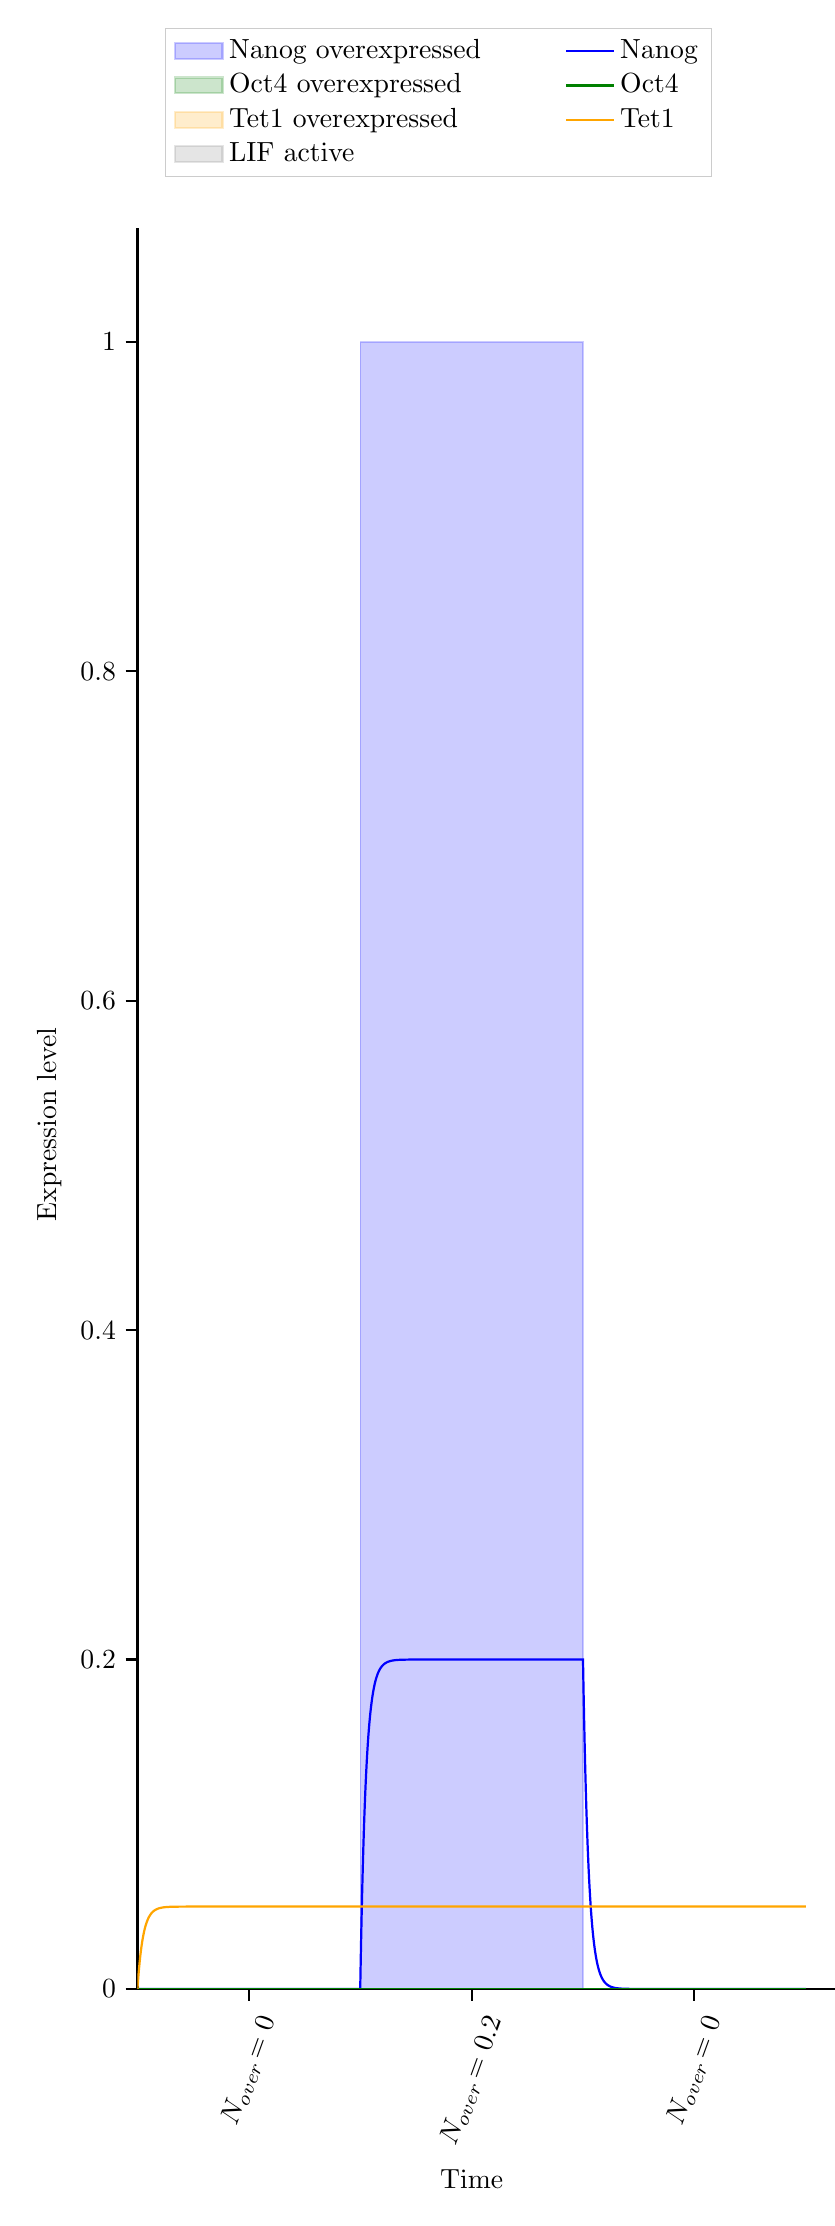
\begin{tikzpicture}[baseline]

\definecolor{darkgray176}{RGB}{176,176,176}
\definecolor{green}{RGB}{0,128,0}
\definecolor{lightgray204}{RGB}{204,204,204}
\definecolor{orange}{RGB}{255,165,0}

\begin{axis}[
 ytick={0,0.2,0.4,0.6,0.8,1},
 x tick label style = {rotate=70},
 y post scale=3, 
 transpose legend,
legend cell align={left},
legend style={fill opacity=0.8, draw opacity=1, text opacity=1, draw=lightgray204, anchor=south west,
    legend columns=4,
    /tikz/every even column/.append style={column sep=1.0cm},, at={(axis cs:5,1.1)}},
tick align=outside,
tick pos=left,
x grid style={darkgray176},
xlabel={Time},
xmin=0, xmax=120,
xtick style={color=black},
xtick={20,60,100},
xticklabels={
  \(\displaystyle N_\text{over}\!=0\),
  \(\displaystyle N_\text{over}\!=0.2\),
  \(\displaystyle N_\text{over}\!=0\)
},
y grid style={darkgray176},
ylabel={Expression level},
ymin=0, ymax=1.05,
ytick style={color=black}
]
\path [draw=blue, fill=blue, opacity=0.2]
(axis cs:40,0)
--(axis cs:40,1)
--(axis cs:80,1)
--(axis cs:80,0)
--cycle;
\addlegendimage{area legend, draw=blue, fill=blue, opacity=0.2}
\addlegendentry{Nanog overexpressed}
\addlegendimage{area legend, draw=green, fill=green, opacity=0.2}
\addlegendentry{Oct4 overexpressed}

\addlegendimage{area legend, draw=orange, fill=orange, opacity=0.2}
\addlegendentry{Tet1 overexpressed}

\addlegendimage{area legend, draw=gray, fill=gray, opacity=0.2}
\addlegendentry{LIF active}

\addplot [thick, blue]
table {%
0 0
0.0001 0
0.0011 0
0.0111 0
0.1111 0
0.2111 0
0.3111 0
0.4111 0
0.5111 0
0.6111 0
0.7111 0
0.8111 0
0.9111 0
1.0111 0
1.1111 0
1.2111 0
1.3111 0
1.4111 0
1.5111 0
1.6111 0
1.7111 0
1.8111 0
1.9111 0
2.0111 0
2.1111 0
2.2111 0
2.3111 0
2.4111 0
2.5111 0
2.6111 0
2.7111 0
2.8111 0
2.9111 0
3.0111 0
3.1111 0
3.2111 0
3.3111 0
3.4111 0
3.5111 0
3.6111 0
3.7111 0
3.8111 0
3.9111 0
4.0111 0
4.1111 0
4.2111 0
4.3111 0
4.4111 0
4.5111 0
4.6111 0
4.7111 0
4.8111 0
4.9111 0
5.0111 0
5.1111 0
5.2111 0
5.3111 0
5.4111 0
5.5111 0
5.6111 0
5.7111 0
5.8111 0
5.9111 0
6.0111 0
6.1111 0
6.21109999999999 0
6.31109999999999 0
6.41109999999999 0
6.51109999999999 0
6.61109999999999 0
6.71109999999999 0
6.81109999999999 0
6.91109999999999 0
7.01109999999999 0
7.11109999999999 0
7.21109999999999 0
7.31109999999999 0
7.41109999999999 0
7.51109999999999 0
7.61109999999999 0
7.71109999999999 0
7.81109999999999 0
7.91109999999999 0
8.01109999999999 0
8.11109999999999 0
8.21109999999999 0
8.31109999999999 0
8.41109999999999 0
8.51109999999999 0
8.61109999999999 0
8.71109999999999 0
8.81109999999999 0
8.91109999999999 0
9.01109999999998 0
9.11109999999998 0
9.21109999999998 0
9.31109999999998 0
9.41109999999998 0
9.51109999999998 0
9.61109999999998 0
9.71109999999998 0
9.81109999999998 0
9.91109999999998 0
10.0111 0
10.1111 0
10.2111 0
10.3111 0
10.4111 0
10.5111 0
10.6111 0
10.7111 0
10.8111 0
10.9111 0
11.0111 0
11.1111 0
11.2111 0
11.3111 0
11.4111 0
11.5111 0
11.6111 0
11.7111 0
11.8111 0
11.9111 0
12.0111 0
12.1111 0
12.2111 0
12.3111 0
12.4111 0
12.5111 0
12.6111 0
12.7111 0
12.8111 0
12.9111 0
13.0111 0
13.1111 0
13.2111 0
13.3111 0
13.4111 0
13.5111 0
13.6111 0
13.7111 0
13.8111 0
13.9111 0
14.0111 0
14.1111 0
14.2111 0
14.3111 0
14.4111 0
14.5111 0
14.6111 0
14.7111 0
14.8111 0
14.9111 0
15.0111 0
15.1111 0
15.2111 0
15.3111 0
15.4111 0
15.5111 0
15.6111 0
15.7111 0
15.8111 0
15.9111 0
16.0111 0
16.1111 0
16.2111 0
16.3111 0
16.4111 0
16.5111 0
16.6111 0
16.7111 0
16.8111 0
16.9111 0
17.0111 0
17.1111 0
17.2111 0
17.3111 0
17.4111 0
17.5111 0
17.6111 0
17.7111 0
17.8111 0
17.9111 0
18.0111 0
18.1111 0
18.2111 0
18.3111 0
18.4111 0
18.5111 0
18.6111 0
18.7111 0
18.8111 0
18.9111 0
19.0111 0
19.1111 0
19.2111 0
19.3111 0
19.4111 0
19.5111 0
19.6111 0
19.7111 0
19.8111 0
19.9111 0
20.0111 0
20.1111 0
20.2111 0
20.3111 0
20.4111 0
20.5111 0
20.6111 0
20.7111 0
20.8111 0
20.9111 0
21.0111 0
21.1111 0
21.2111 0
21.3111 0
21.4111 0
21.5111 0
21.6111 0
21.7111 0
21.8111 0
21.9111 0
22.0111 0
22.1111 0
22.2111 0
22.3111 0
22.4111000000001 0
22.5111000000001 0
22.6111000000001 0
22.7111000000001 0
22.8111000000001 0
22.9111000000001 0
23.0111000000001 0
23.1111000000001 0
23.2111000000001 0
23.3111000000001 0
23.4111000000001 0
23.5111000000001 0
23.6111000000001 0
23.7111000000001 0
23.8111000000001 0
23.9111000000001 0
24.0111000000001 0
24.1111000000001 0
24.2111000000001 0
24.3111000000001 0
24.4111000000001 0
24.5111000000001 0
24.6111000000001 0
24.7111000000001 0
24.8111000000001 0
24.9111000000001 0
25.0111000000001 0
25.1111000000001 0
25.2111000000001 0
25.3111000000001 0
25.4111000000001 0
25.5111000000001 0
25.6111000000001 0
25.7111000000001 0
25.8111000000001 0
25.9111000000001 0
26.0111000000001 0
26.1111000000001 0
26.2111000000001 0
26.3111000000001 0
26.4111000000001 0
26.5111000000001 0
26.6111000000001 0
26.7111000000001 0
26.8111000000001 0
26.9111000000001 0
27.0111000000001 0
27.1111000000001 0
27.2111000000001 0
27.3111000000001 0
27.4111000000001 0
27.5111000000001 0
27.6111000000001 0
27.7111000000001 0
27.8111000000001 0
27.9111000000001 0
28.0111000000001 0
28.1111000000001 0
28.2111000000001 0
28.3111000000001 0
28.4111000000001 0
28.5111000000001 0
28.6111000000001 0
28.7111000000001 0
28.8111000000001 0
28.9111000000001 0
29.0111000000001 0
29.1111000000001 0
29.2111000000001 0
29.3111000000001 0
29.4111000000002 0
29.5111000000002 0
29.6111000000002 0
29.7111000000002 0
29.8111000000002 0
29.9111000000002 0
30.0111000000002 0
30.1111000000002 0
30.2111000000002 0
30.3111000000002 0
30.4111000000002 0
30.5111000000002 0
30.6111000000002 0
30.7111000000002 0
30.8111000000002 0
30.9111000000002 0
31.0111000000002 0
31.1111000000002 0
31.2111000000002 0
31.3111000000002 0
31.4111000000002 0
31.5111000000002 0
31.6111000000002 0
31.7111000000002 0
31.8111000000002 0
31.9111000000002 0
32.0111000000002 0
32.1111000000002 0
32.2111000000002 0
32.3111000000002 0
32.4111000000002 0
32.5111000000002 0
32.6111000000002 0
32.7111000000002 0
32.8111000000002 0
32.9111000000002 0
33.0111000000002 0
33.1111000000002 0
33.2111000000002 0
33.3111000000002 0
33.4111000000002 0
33.5111000000002 0
33.6111000000002 0
33.7111000000002 0
33.8111000000002 0
33.9111000000002 0
34.0111000000002 0
34.1111000000002 0
34.2111000000002 0
34.3111000000002 0
34.4111000000002 0
34.5111000000002 0
34.6111000000002 0
34.7111000000002 0
34.8111000000002 0
34.9111000000002 0
35.0111000000002 0
35.1111000000002 0
35.2111000000002 0
35.3111000000002 0
35.4111000000002 0
35.5111000000002 0
35.6111000000002 0
35.7111000000002 0
35.8111000000002 0
35.9111000000002 0
36.0111000000002 0
36.1111000000002 0
36.2111000000002 0
36.3111000000002 0
36.4111000000002 0
36.5111000000002 0
36.6111000000002 0
36.7111000000003 0
36.8111000000003 0
36.9111000000003 0
37.0111000000003 0
37.1111000000003 0
37.2111000000003 0
37.3111000000003 0
37.4111000000003 0
37.5111000000003 0
37.6111000000003 0
37.7111000000003 0
37.8111000000003 0
37.9111000000003 0
38.0111000000003 0
38.1111000000003 0
38.2111000000003 0
38.3111000000003 0
38.4111000000003 0
38.5111000000003 0
38.6111000000003 0
38.7111000000003 0
38.8111000000003 0
38.9111000000003 0
39.0111000000003 0
39.1111000000003 0
39.2111000000003 0
39.3111000000003 0
39.4111000000003 0
39.5111000000003 0
39.6111000000003 0
39.7111000000003 0
39.8111000000003 0
39.9111000000003 0
40 0
40 0
40.0049019607843 0.000977993156446256
40.0539215686275 0.0104987164359239
40.1539215686275 0.0285321478090287
40.2539215686275 0.0448494712963602
40.3539215686275 0.059613996154747
40.4539215686275 0.0729734907105281
40.5539215686275 0.0850616612746192
40.6539215686275 0.0959994903202044
40.7539215686275 0.105896447315983
40.8539215686275 0.114851584333399
40.9539215686275 0.12295452739306
41.0539215686275 0.130286373472065
41.1539215686275 0.136920502149809
41.2539215686275 0.14292331001547
41.3539215686275 0.148354875187386
41.4539215686275 0.153269558595052
41.5539215686275 0.157716548041569
41.6539215686275 0.161740350491712
41.7539215686275 0.165381237512583
41.8539215686275 0.168675648324991
41.9539215686275 0.171656554499419
42.0539215686275 0.174353789946583
42.1539215686275 0.176794349505232
42.2539215686275 0.179002659115568
42.3539215686275 0.181000820282266
42.4539215686275 0.182808831273754
42.5539215686275 0.184444787271611
42.6539215686275 0.185925061473219
42.7539215686275 0.187264468960227
42.8539215686275 0.188476414972868
42.9539215686275 0.189573029074105
43.0539215686275 0.190565286546377
43.1539215686275 0.191463118235909
43.2539215686275 0.192275509943963
43.3539215686275 0.193010592359754
43.4539215686275 0.19367572243512
43.5539215686275 0.194277557015371
43.6539215686275 0.194822119463228
43.7539215686275 0.195314859942669
43.8539215686275 0.195760709965995
43.9539215686275 0.196164131750064
44.0539215686275 0.196529162875662
44.1539215686275 0.196859456696958
44.2539215686275 0.197158318905512
44.3539215686275 0.197428740614736
44.4539215686275 0.197673428295973
44.5539215686275 0.197894830865761
44.6539215686275 0.19809516419542
44.7539215686275 0.198276433288235
44.8539215686275 0.198440452346201
44.9539215686275 0.198588862927169
45.0539215686276 0.198723150374105
45.1539215686276 0.198844658680905
45.2539215686276 0.198954603943537
45.3539215686276 0.199054086531134
45.4539215686276 0.199144102098864
45.5539215686276 0.199225551552779
45.6539215686276 0.199299250066385
45.7539215686276 0.19936593523917
45.8539215686276 0.199426274478755
45.9539215686276 0.199480871680524
46.0539215686276 0.199530273271622
46.1539215686276 0.199574973679772
46.2539215686276 0.199615420281681
46.3539215686276 0.199652017880533
46.4539215686276 0.199685132757396
46.5539215686276 0.199715096337084
46.6539215686276 0.199742208505173
46.7539215686276 0.199766740609353
46.8539215686276 0.199788938175165
46.9539215686276 0.199809023363307
47.0539215686276 0.199827197193093
47.1539215686276 0.199843641554318
47.2539215686276 0.199858521027674
47.3539215686276 0.199871984531932
47.4539215686276 0.199884166814367
47.5539215686276 0.199895189799354
47.6539215686276 0.199905163808633
47.7539215686276 0.199914188665439
47.8539215686276 0.199922354693572
47.9539215686276 0.199929743621386
48.0539215686276 0.199936429399753
48.1539215686276 0.199942478942191
48.2539215686276 0.199947952794552
48.3539215686276 0.199952905740991
48.4539215686276 0.19995738735226
48.5539215686276 0.199961442481831
48.6539215686276 0.199965111714802
48.7539215686276 0.199968431774092
48.8539215686276 0.199971435887968
48.9539215686276 0.199974154122612
49.0539215686276 0.199976613683029
49.1539215686276 0.199978839185328
49.2539215686276 0.199980852903082
49.3539215686276 0.199982674990257
49.4539215686276 0.199984323682911
49.5539215686276 0.199985815481716
49.6539215686276 0.199987165317096
49.7539215686276 0.199988386698656
49.8539215686276 0.199989491850393
49.9539215686276 0.199990491833039
50.0539215686276 0.199991396654754
50.1539215686276 0.199992215371298
50.2539215686276 0.199992956176663
50.3539215686276 0.199993626485076
50.4539215686276 0.199994233005211
50.5539215686276 0.199994781807323
50.6539215686276 0.19999527838401
50.7539215686276 0.199995727705177
50.8539215686276 0.199996134267782
50.9539215686276 0.19999650214084
51.0539215686276 0.199996835006148
51.1539215686276 0.199997136195134
51.2539215686276 0.199997408722199
51.3539215686276 0.199997655314884
51.4539215686276 0.199997878441173
51.5539215686276 0.199998080334188
51.6539215686276 0.199998263014543
51.7539215686276 0.199998428310563
51.8539215686276 0.199998577876587
51.9539215686276 0.199998713209523
52.0539215686277 0.199998835663827
52.1539215686277 0.199998946465063
52.2539215686277 0.199999046722167
52.3539215686277 0.199999137438547
52.4539215686277 0.199999219522122
52.5539215686277 0.199999293794412
52.6539215686277 0.199999360998759
52.7539215686277 0.199999421807766
52.8539215686277 0.199999476830032
52.9539215686277 0.199999526616237
53.0539215686277 0.199999571664658
53.1539215686277 0.199999612426155
53.2539215686277 0.199999649308682
53.3539215686277 0.199999682681374
53.4539215686277 0.199999712878233
53.5539215686277 0.199999740201482
53.6539215686277 0.19999976492458
53.7539215686277 0.199999787294964
53.8539215686277 0.199999807536524
53.9539215686277 0.199999825851845
54.0539215686277 0.199999842424233
54.1539215686277 0.19999985741955
54.2539215686277 0.199999870987874
54.3539215686277 0.199999883265001
54.4539215686277 0.199999894373805
54.5539215686277 0.199999904425466
54.6539215686277 0.199999913520585
54.7539215686277 0.19999992175019
54.8539215686277 0.199999929196644
54.9539215686277 0.199999935934474
55.0539215686277 0.199999942031115
55.1539215686277 0.199999947547584
55.2539215686277 0.199999952539091
55.3539215686277 0.199999957055594
55.4539215686277 0.199999961142294
55.5539215686277 0.199999964840094
55.6539215686277 0.199999968186001
55.7539215686277 0.199999971213503
55.8539215686277 0.199999973952901
55.9539215686277 0.19999997643161
56.0539215686277 0.199999978674439
56.1539215686277 0.199999980703834
56.2539215686277 0.199999982540107
56.3539215686277 0.199999984201636
56.4539215686277 0.199999985705049
56.5539215686277 0.199999987065393
56.6539215686277 0.199999988296284
56.7539215686277 0.19999998941004
56.8539215686277 0.199999990417808
56.9539215686277 0.199999991329674
57.0539215686277 0.199999992154764
57.1539215686277 0.199999992901337
57.2539215686277 0.199999993576864
57.3539215686277 0.199999994188107
57.4539215686277 0.199999994741181
57.5539215686277 0.199999995241624
57.6539215686277 0.199999995694443
57.7539215686277 0.199999996104171
57.8539215686277 0.199999996474908
57.9539215686277 0.199999996810365
58.0539215686277 0.199999997113899
58.1539215686277 0.199999997388548
58.2539215686277 0.19999999763706
58.3539215686277 0.199999997861924
58.4539215686277 0.199999998065389
58.5539215686277 0.199999998249491
58.6539215686277 0.199999998416074
58.7539215686277 0.199999998566805
58.8539215686277 0.199999998703191
58.9539215686277 0.199999998826599
59.0539215686278 0.199999998938263
59.1539215686278 0.1999999990393
59.2539215686278 0.199999999130723
59.3539215686278 0.199999999213446
59.4539215686278 0.199999999288296
59.5539215686278 0.199999999356024
59.6539215686278 0.199999999417306
59.7539215686278 0.199999999472757
59.8539215686278 0.199999999522931
59.9539215686278 0.19999999956833
60.0539215686278 0.199999999609409
60.1539215686278 0.199999999646578
60.2539215686278 0.199999999680211
60.3539215686278 0.199999999710643
60.4539215686278 0.199999999738179
60.5539215686278 0.199999999763094
60.6539215686278 0.199999999785639
60.7539215686278 0.199999999806038
60.8539215686278 0.199999999824496
60.9539215686278 0.199999999841197
61.0539215686278 0.19999999985631
61.1539215686278 0.199999999869983
61.2539215686278 0.199999999882356
61.3539215686278 0.199999999893551
61.4539215686278 0.199999999903681
61.5539215686278 0.199999999912847
61.6539215686278 0.199999999921141
61.7539215686278 0.199999999928645
61.8539215686278 0.199999999935436
61.9539215686278 0.19999999994158
62.0539215686278 0.199999999947139
62.1539215686278 0.19999999995217
62.2539215686278 0.199999999956721
62.3539215686278 0.19999999996084
62.4539215686278 0.199999999964566
62.5539215686278 0.199999999967938
62.6539215686278 0.199999999970989
62.7539215686278 0.19999999997375
62.8539215686278 0.199999999976248
62.9539215686278 0.199999999978508
63.0539215686278 0.199999999980554
63.1539215686278 0.199999999982404
63.2539215686278 0.199999999984079
63.3539215686278 0.199999999985594
63.4539215686278 0.199999999986965
63.5539215686278 0.199999999988205
63.6539215686278 0.199999999989328
63.7539215686278 0.199999999990343
63.8539215686278 0.199999999991262
63.9539215686278 0.199999999992094
64.0539215686278 0.199999999992846
64.1539215686278 0.199999999993527
64.2539215686278 0.199999999994143
64.3539215686278 0.1999999999947
64.4539215686278 0.199999999995205
64.5539215686278 0.199999999995661
64.6539215686278 0.199999999996074
64.7539215686278 0.199999999996447
64.8539215686278 0.199999999996786
64.9539215686278 0.199999999997091
65.0539215686278 0.199999999997368
65.1539215686278 0.199999999997619
65.2539215686277 0.199999999997845
65.3539215686277 0.19999999999805
65.4539215686277 0.199999999998236
65.5539215686277 0.199999999998404
65.6539215686277 0.199999999998556
65.7539215686277 0.199999999998693
65.8539215686277 0.199999999998817
65.9539215686277 0.19999999999893
66.0539215686277 0.199999999999032
66.1539215686277 0.199999999999124
66.2539215686277 0.199999999999207
66.3539215686277 0.199999999999283
66.4539215686277 0.199999999999351
66.5539215686277 0.199999999999413
66.6539215686277 0.199999999999469
66.7539215686277 0.199999999999519
66.8539215686277 0.199999999999565
66.9539215686276 0.199999999999606
67.0539215686276 0.199999999999644
67.1539215686276 0.199999999999678
67.2539215686276 0.199999999999708
67.3539215686276 0.199999999999736
67.4539215686276 0.199999999999761
67.5539215686276 0.199999999999784
67.6539215686276 0.199999999999805
67.7539215686276 0.199999999999823
67.8539215686276 0.19999999999984
67.9539215686276 0.199999999999855
68.0539215686276 0.199999999999869
68.1539215686276 0.199999999999881
68.2539215686276 0.199999999999893
68.3539215686276 0.199999999999903
68.4539215686276 0.199999999999912
68.5539215686276 0.199999999999921
68.6539215686276 0.199999999999928
68.7539215686275 0.199999999999935
68.8539215686275 0.199999999999941
68.9539215686275 0.199999999999947
69.0539215686275 0.199999999999952
69.1539215686275 0.199999999999956
69.2539215686275 0.199999999999961
69.3539215686275 0.199999999999964
69.4539215686275 0.199999999999968
69.5539215686275 0.199999999999971
69.6539215686275 0.199999999999974
69.7539215686275 0.199999999999976
69.8539215686275 0.199999999999978
69.9539215686275 0.19999999999998
70.0539215686275 0.199999999999982
70.1539215686275 0.199999999999984
70.2539215686275 0.199999999999985
70.3539215686275 0.199999999999987
70.4539215686275 0.199999999999988
70.5539215686274 0.199999999999989
70.6539215686274 0.19999999999999
70.7539215686274 0.199999999999991
70.8539215686274 0.199999999999992
70.9539215686274 0.199999999999993
71.0539215686274 0.199999999999993
71.1539215686274 0.199999999999994
71.2539215686274 0.199999999999995
71.3539215686274 0.199999999999995
71.4539215686274 0.199999999999996
71.5539215686274 0.199999999999996
71.6539215686274 0.199999999999996
71.7539215686274 0.199999999999997
71.8539215686274 0.199999999999997
71.9539215686274 0.199999999999997
72.0539215686274 0.199999999999998
72.1539215686274 0.199999999999998
72.2539215686273 0.199999999999998
72.3539215686273 0.199999999999998
72.4539215686273 0.199999999999998
72.5539215686273 0.199999999999999
72.6539215686273 0.199999999999999
72.7539215686273 0.199999999999999
72.8539215686273 0.199999999999999
72.9539215686273 0.199999999999999
73.0539215686273 0.199999999999999
73.1539215686273 0.199999999999999
73.2539215686273 0.199999999999999
73.3539215686273 0.199999999999999
73.4539215686273 0.199999999999999
73.5539215686273 0.199999999999999
73.6539215686273 0.2
73.7539215686273 0.2
73.8539215686273 0.2
73.9539215686273 0.2
74.0539215686272 0.2
74.1539215686272 0.2
74.2539215686272 0.2
74.3539215686272 0.2
74.4539215686272 0.2
74.5539215686272 0.2
74.6539215686272 0.2
74.7539215686272 0.2
74.8539215686272 0.2
74.9539215686272 0.2
75.0539215686272 0.2
75.1539215686272 0.2
75.2539215686272 0.2
75.3539215686272 0.2
75.4539215686272 0.2
75.5539215686272 0.2
75.6539215686272 0.2
75.7539215686271 0.2
75.8539215686271 0.2
75.9539215686271 0.2
76.0539215686271 0.2
76.1539215686271 0.2
76.2539215686271 0.2
76.3539215686271 0.2
76.4539215686271 0.2
76.5539215686271 0.2
76.6539215686271 0.2
76.7539215686271 0.2
76.8539215686271 0.2
76.9539215686271 0.2
77.0539215686271 0.2
77.1539215686271 0.2
77.2539215686271 0.2
77.3539215686271 0.2
77.4539215686271 0.2
77.553921568627 0.2
77.653921568627 0.2
77.753921568627 0.2
77.853921568627 0.2
77.953921568627 0.2
78.053921568627 0.2
78.153921568627 0.2
78.253921568627 0.2
78.353921568627 0.2
78.453921568627 0.2
78.553921568627 0.2
78.653921568627 0.2
78.753921568627 0.2
78.853921568627 0.2
78.953921568627 0.2
79.053921568627 0.2
79.153921568627 0.2
79.253921568627 0.2
79.3539215686269 0.2
79.4539215686269 0.2
79.5539215686269 0.2
79.6539215686269 0.2
79.7539215686269 0.2
79.8539215686269 0.2
79.9539215686269 0.2
80 0.2
80 0.2
80.1 0.180967483666668
80.2 0.163746150723228
80.3 0.148163644282427
80.4 0.134064009383371
80.5 0.121306132141866
80.6 0.109762327435249
80.7 0.0993170609867688
80.8 0.0898657930597227
80.8999999999999 0.0813139321886375
80.9999999999999 0.0735758884760989
81.0999999999999 0.066574216980295
81.1999999999999 0.0602388426200136
81.2999999999999 0.0545063588396814
81.3999999999999 0.0493193930152478
81.4999999999999 0.0446260322496841
81.5999999999999 0.0403793038112645
81.6999999999999 0.0365367050146821
81.7999999999999 0.0330597778398917
81.8999999999999 0.0299137240313213
81.9999999999999 0.0270670568252367
82.0999999999999 0.024491285819629
82.1999999999999 0.022160631832697
82.2999999999999 0.0200517688961331
82.3999999999999 0.0181435908009938
82.4999999999999 0.0164169998596678
82.5999999999999 0.0148547157698006
82.6999999999998 0.0134411026672219
82.7999999999998 0.0121620126369624
82.8999999999998 0.0110046441161665
82.9999999999998 0.00995741377174925
83.0999999999998 0.00900984057050642
83.1999999999998 0.00815244088141201
83.2999999999998 0.00737663356025201
83.3999999999998 0.00667465406664949
83.4999999999998 0.00603947675393524
83.5999999999998 0.00546474455411498
83.6999999999998 0.00494470535419657
83.7999999999998 0.00447415442711026
83.8999999999998 0.00404838234105112
83.9999999999998 0.00366312782590297
84.0999999999998 0.00331453512501506
84.1999999999998 0.0029991154054938
84.2999999999998 0.00271371184079075
84.3999999999997 0.00245546801612172
84.4999999999997 0.00222179934050766
84.5999999999997 0.00201036717931966
84.6999999999997 0.00181905544843768
84.7999999999997 0.00164594943576954
84.8999999999997 0.00148931663816893
84.9999999999997 0.00134758942196166
85.0999999999997 0.0012193493335411
85.1999999999997 0.00110331290300781
85.2999999999997 0.000998318798771448
85.3999999999997 0.000903316204553996
85.4999999999997 0.000817354302467308
85.5999999999997 0.000739572756908166
85.6999999999997 0.000669193104030454
85.7999999999997 0.000605510960617389
85.8999999999997 0.000547888974377578
85.9999999999997 0.000495750445109109
86.0999999999997 0.000448573552890129
86.1999999999996 0.000405886135529718
86.2999999999996 0.000367260963010006
86.3999999999996 0.000332311461624589
86.4999999999996 0.000300687845018971
86.5999999999996 0.000272073613411181
86.6999999999996 0.000246182385955596
86.7999999999996 0.000222755034547203
86.8999999999996 0.000201557090380445
86.9999999999996 0.000182376397306621
87.0999999999996 0.000165020988503858
87.1999999999996 0.000149317165208647
87.2999999999996 0.000135107758280244
87.3999999999996 0.000122250555199101
87.4999999999996 0.000110616876756172
87.5999999999996 0.000100090289188152
87.6999999999996 9.05654388692443e-05
87.7999999999996 8.19469978966728e-05
87.8999999999996 7.4148710016993e-05
87.9999999999995 6.70925273445233e-05
88.0999999999995 6.07078292318773e-05
88.1999999999995 5.49307154747931e-05
88.2999999999995 4.97033667774149e-05
88.3999999999995 4.49734660773511e-05
88.4999999999995 4.06936749389324e-05
88.5999999999995 3.68211597742397e-05
88.6999999999995 3.33171631501624e-05
88.7999999999995 3.01466158909836e-05
88.8999999999995 2.72777860942844e-05
88.9999999999995 2.46819615474013e-05
89.0999999999995 2.23331623659533e-05
89.1999999999995 2.02078809784285e-05
89.2999999999995 1.82848468545086e-05
89.3999999999995 1.6544813622454e-05
89.4999999999995 1.49703664449476e-05
89.5999999999995 1.35457477255504e-05
89.6999999999994 1.22566994013817e-05
89.7999999999994 1.1090320243634e-05
89.8999999999994 1.00349367377397e-05
89.9999999999994 9.07998625091481e-06
90.0999999999994 8.21591131777996e-06
90.1999999999994 7.43406398603568e-06
90.2999999999994 6.72661926484937e-06
90.3999999999994 6.08649680971761e-06
90.4999999999994 5.50729005999898e-06
90.5999999999994 4.98320211990233e-06
90.6999999999994 4.50898774120565e-06
90.7999999999994 4.07990082704919e-06
90.8999999999994 3.69164693140324e-06
90.9999999999994 3.3403402788091e-06
91.0999999999994 3.02246487423249e-06
91.1999999999994 2.73483931380372e-06
91.2999999999994 2.47458494425868e-06
91.3999999999994 2.23909705240957e-06
91.4999999999993 2.02601879630007e-06
91.5999999999993 1.83321761713897e-06
91.6999999999993 1.65876389593522e-06
91.7999999999993 1.50091164122257e-06
91.8999999999993 1.35808101459029e-06
91.9999999999993 1.2288425191294e-06
92.0999999999993 1.11190269254728e-06
92.1999999999993 1.00609116176237e-06
92.2999999999993 9.10348929417051e-07
92.3999999999993 8.23717775076243e-07
92.4999999999993 7.45330665035269e-07
92.5999999999993 6.74403074755183e-07
92.6999999999993 6.10225137077545e-07
92.7999999999993 5.52154537635354e-07
92.8999999999993 4.99610086355012e-07
92.9999999999993 4.52065900710765e-07
93.0999999999993 4.09046142515664e-07
93.1999999999992 3.70120255573084e-07
93.2999999999992 3.34898656525625e-07
93.3999999999992 3.0302883577395e-07
93.4999999999992 2.74191829442258e-07
93.5999999999992 2.48099027080628e-07
93.6999999999992 2.24489283154648e-07
93.7999999999992 2.03126303413154e-07
93.8999999999992 1.83796279975952e-07
93.9999999999992 1.66305751472712e-07
94.0999999999992 1.50479666816555e-07
94.1999999999992 1.36159633233952e-07
94.2999999999992 1.23202331016624e-07
94.3999999999992 1.11478079129731e-07
94.4999999999992 1.00869537320506e-07
94.5999999999992 9.12705317375646e-08
94.6999999999992 8.2584992307329e-08
94.7999999999992 7.47259912324422e-08
94.8999999999992 6.76148729891627e-08
94.9999999999991 6.11804671164505e-08
95.0999999999991 5.53583759180768e-08
95.1999999999991 5.00903299488391e-08
95.2999999999991 4.53236048343727e-08
95.3999999999991 4.10104935878942e-08
95.4999999999991 3.71078291426461e-08
95.5999999999991 3.35765523213865e-08
95.6999999999991 3.03813209190176e-08
95.7999999999991 2.74901559859206e-08
95.8999999999991 2.48741217718811e-08
95.9999999999991 2.2507036127378e-08
96.0999999999991 2.03652084638319e-08
96.1999999999991 1.84272026502339e-08
96.2999999999991 1.66736224731429e-08
96.3999999999991 1.50869175128634e-08
96.4999999999991 1.36512074929473e-08
96.5999999999991 1.23521233450512e-08
96.6999999999991 1.11766633984711e-08
96.799999999999 1.01130632550533e-08
96.899999999999 9.15067804714416e-09
96.999999999999 8.27987590017748e-09
97.099999999999 7.49194153363701e-09
97.199999999999 6.77898903560043e-09
97.299999999999 6.1338829378827e-09
97.399999999999 5.55016680187269e-09
97.499999999999 5.02199860032589e-09
97.599999999999 4.54409224839252e-09
97.699999999999 4.11166469870402e-09
97.799999999999 3.72038807102767e-09
97.899999999999 3.36634633738683e-09
97.999999999999 3.04599612913699e-09
98.099999999999 2.75613127374165e-09
98.199999999999 2.49385070632017e-09
98.299999999999 2.25652943481552e-09
98.399999999999 2.04179226819166e-09
98.4999999999989 1.84749004472351e-09
98.5999999999989 1.67167812246417e-09
98.6999999999989 1.5125969166148e-09
98.7999999999989 1.3686542890087e-09
98.8999999999989 1.23840961345749e-09
98.9999999999989 1.12055935748006e-09
99.0999999999989 1.01392403611152e-09
99.1999999999989 9.17436407221268e-10
99.2999999999989 8.30130790195106e-10
99.3999999999989 7.51133401079154e-10
99.4999999999989 6.79653607456401e-10
99.5999999999989 6.1497601553179e-10
99.6999999999989 5.56453310230708e-10
99.7999999999989 5.03499776652194e-10
99.8999999999989 4.55585438037384e-10
99.9999999999989 4.1223075158401e-10
100.099999999999 3.73001809020887e-10
100.199999999999 3.37505993908125e-10
100.299999999999 3.05388052199855e-10
100.399999999999 2.76326536742364e-10
100.499999999999 2.50030590122953e-10
100.599999999999 2.26237033671214e-10
100.699999999999 2.04707733478453e-10
100.799999999999 1.85227217073513e-10
100.899999999999 1.67600516901866e-10
100.999999999999 1.51651219024818e-10
101.099999999999 1.3721969750952e-10
101.199999999999 1.24161516838996e-10
101.299999999999 1.12345986352948e-10
101.399999999999 1.01654852251714e-10
101.499999999999 9.19811140724978e-11
101.599999999999 8.32279537927832e-11
101.699999999999 7.53077668430284e-11
101.799999999999 6.81412853306948e-11
101.899999999999 6.16567847005413e-11
101.999999999999 5.57893658911722e-11
102.099999999999 5.04803058034223e-11
102.199999999999 4.56764695798461e-11
102.299999999999 4.13297788132092e-11
102.399999999999 3.73967303616321e-11
102.499999999999 3.38379609545272e-11
102.599999999999 3.06178532317587e-11
102.699999999999 2.77041792731336e-11
102.799999999999 2.50677780505462e-11
102.899999999999 2.26822635746093e-11
102.999999999999 2.05237608148058e-11
103.099999999999 1.85706667501598e-11
103.199999999999 1.68034341589434e-11
103.299999999999 1.52043759835126e-11
103.399999999999 1.37574883122909e-11
103.499999999999 1.24482902072444e-11
103.599999999999 1.12636787737872e-11
103.699999999999 1.01917980226096e-11
103.799999999999 9.22192021095293e-12
103.899999999999 8.34433847575469e-12
103.999999999999 7.55026968410142e-12
104.099999999999 6.8317665286828e-12
104.199999999999 6.18163798846945e-12
104.299999999999 5.59337735855799e-12
104.399999999999 5.06109712888176e-12
104.499999999999 4.57947006003165e-12
104.599999999999 4.14367586645385e-12
104.699999999999 3.74935297341226e-12
104.799999999999 3.39255486488278e-12
104.899999999999 3.06971058549474e-12
104.999999999999 2.77758900120958e-12
105.099999999999 2.51326646104555e-12
105.199999999999 2.27409753619623e-12
105.299999999999 2.05768854369e-12
105.399999999999 1.86187358960655e-12
105.499999999999 1.68469289208261e-12
105.599999999999 1.52437316715656e-12
105.699999999999 1.37930988114655e-12
105.799999999999 1.24805119193831e-12
105.899999999999 1.12928341846131e-12
105.999999999999 1.02181789292718e-12
106.099999999999 9.24579064243038e-13
106.199999999999 8.36593733534725e-13
106.299999999999 7.56981314045409e-13
106.399999999998 6.84945017927426e-13
106.499999999998 6.19763881721734e-13
106.599999999998 5.60785550713343e-13
106.699999999998 5.07419749946101e-13
106.799999999998 4.59132376552578e-13
106.899999999998 4.15440154273085e-13
106.999999999998 3.75905796664462e-13
107.099999999998 3.40133630590408e-13
107.199999999998 3.07765636191771e-13
107.299999999998 2.78477863703479e-13
107.399999999998 2.51977191256439e-13
107.499999999998 2.27998391215363e-13
107.599999999998 2.06301475691463e-13
107.699999999998 1.86669294663022e-13
107.799999999998 1.68905362664994e-13
107.899999999998 1.52831892296449e-13
107.999999999998 1.38288014864518e-13
108.099999999998 1.25128170356453e-13
108.199999999998 1.13220650626107e-13
108.299999999998 1.02446281214547e-13
108.399999999998 9.26972286120222e-14
108.499999999998 8.38759210239575e-14
108.599999999998 7.58940718396487e-14
108.699999999998 6.86717960301926e-14
108.799999999998 6.21368106322731e-14
108.899999999998 5.62237113159735e-14
108.999999999998 5.08733177962644e-14
109.099999999998 4.60320815368233e-14
109.199999999998 4.1651549818289e-14
109.299999999998 3.7687880807163e-14
109.399999999998 3.4101404772008e-14
109.499999999998 3.08562270554439e-14
109.599999999998 2.79198688283552e-14
109.699999999998 2.52629420308543e-14
109.799999999998 2.2858855246703e-14
109.899999999998 2.06835475674822e-14
109.999999999998 1.87152477829354e-14
110.099999999998 1.693425648738e-14
110.199999999998 1.53227489214355e-14
110.299999999998 1.38645965758417e-14
110.399999999998 1.25452057719178e-14
110.499999999998 1.13513716031226e-14
110.599999999998 1.02711457759119e-14
110.699999999998 9.29371702720145e-15
110.799999999998 8.40930292161355e-15
110.899999999998 7.60905194557581e-15
110.999999999998 6.88495491839908e-15
111.099999999998 6.22976483370564e-15
111.199999999998 5.63692432895403e-15
111.299999999998 5.10050005715115e-15
111.399999999998 4.6151233039217e-15
111.499999999998 4.17593625561054e-15
111.599999999998 3.77854338065123e-15
111.699999999998 3.41896743760898e-15
111.799999999998 3.09360966961186e-15
111.899999999998 2.79921378678265e-15
111.999999999998 2.5328333761955e-15
112.099999999998 2.29180241318525e-15
112.199999999998 2.07370857887665e-15
112.299999999998 1.87636911688645e-15
112.399999999998 1.69780898756394e-15
112.499999999998 1.53624110113049e-15
112.599999999998 1.39004843188448e-15
112.699999999998 1.25776783446466e-15
112.799999999998 1.13807540019972e-15
112.899999999998 1.02977320698539e-15
112.999999999998 9.31777330077506e-16
113.099999999998 8.43106993808861e-16
113.199999999998 7.62874755656792e-16
113.299999999998 6.90277624420168e-16
113.399999999998 6.24589023613615e-16
113.499999999998 5.65151519645884e-16
113.599999999998 5.11370242003544e-16
113.699999999998 4.62706929586982e-16
113.799999999998 4.1867454361243e-16
113.899999999998 3.7883239316416e-16
113.999999999998 3.42781724611699e-16
114.099999999998 3.10161730749499e-16
114.199999999998 2.80645939717177e-16
114.299999999998 2.53938947559424e-16
114.399999999998 2.29773461723954e-16
114.499999999998 2.07907625907817e-16
114.599999999998 1.88122599478243e-16
114.699999999998 1.7022036724205e-16
114.799999999998 1.54021757643049e-16
114.899999999998 1.393646495529e-16
114.999999999998 1.26102349708376e-16
115.099999999998 1.14102124555895e-16
115.199999999998 1.03243871809505e-16
115.299999999998 9.34189184268506e-17
115.399999999998 8.45289329728442e-17
115.499999999998 7.64849414856202e-17
115.599999999998 6.9206436995225e-17
115.699999999998 6.26205737828083e-17
115.799999999998 5.66614383161886e-17
115.899999999998 5.12693895650738e-17
115.999999999998 4.63904620935875e-17
116.099999999998 4.19758259560524e-17
116.199999999998 3.7981297990484e-17
116.299999999998 3.43668996186587e-17
116.399999999998 3.10964567270681e-17
116.499999999998 2.81372376242347e-17
116.599999999998 2.54596254509442e-17
116.699999999998 2.30368217647661e-17
116.799999999998 2.08445783322362e-17
116.899999999998 1.88609544443877e-17
116.999999999998 1.70660973267625e-17
117.099999999998 1.54420434461732e-17
117.199999999998 1.39725387256266e-17
117.299999999998 1.26428758680586e-17
117.399999999998 1.1439747160763e-17
117.499999999998 1.03511112873309e-17
117.599999999998 9.36607281410961e-18
117.699999999998 8.47477314504101e-18
117.799999999998 7.66829185351961e-18
117.899999999998 6.93855740376526e-18
117.999999999998 6.27826636818063e-18
118.099999999998 5.68081033219358e-18
118.199999999998 5.1402097550234e-18
118.299999999998 4.65105412442721e-18
118.399999999998 4.20844780647535e-18
118.499999999998 3.80796104840175e-18
118.599999999998 3.44558564414976e-18
118.699999999998 3.11769481889888e-18
118.799999999998 2.82100693108369e-18
118.899999999998 2.55255262862222e-18
118.999999999998 2.3096451306425e-18
119.099999999998 2.08985333727673e-18
119.199999999998 1.89097749839679e-18
119.299999999998 1.71102719777578e-18
119.399999999998 1.54820143233357e-18
119.499999999998 1.40087058709268e-18
119.599999999998 1.26756012544405e-18
119.699999999998 1.14693583148908e-18
119.799999999998 1.03779045675858e-18
119.899999999998 9.39031637664407e-19
119.999999999998 8.49670962757589e-19
120 8.49670962755657e-19
};
\addlegendentry{Nanog}
\addplot [thick, green]
table {%
0 0
0.0001 0
0.0011 0
0.0111 0
0.1111 0
0.2111 0
0.3111 0
0.4111 0
0.5111 0
0.6111 0
0.7111 0
0.8111 0
0.9111 0
1.0111 0
1.1111 0
1.2111 0
1.3111 0
1.4111 0
1.5111 0
1.6111 0
1.7111 0
1.8111 0
1.9111 0
2.0111 0
2.1111 0
2.2111 0
2.3111 0
2.4111 0
2.5111 0
2.6111 0
2.7111 0
2.8111 0
2.9111 0
3.0111 0
3.1111 0
3.2111 0
3.3111 0
3.4111 0
3.5111 0
3.6111 0
3.7111 0
3.8111 0
3.9111 0
4.0111 0
4.1111 0
4.2111 0
4.3111 0
4.4111 0
4.5111 0
4.6111 0
4.7111 0
4.8111 0
4.9111 0
5.0111 0
5.1111 0
5.2111 0
5.3111 0
5.4111 0
5.5111 0
5.6111 0
5.7111 0
5.8111 0
5.9111 0
6.0111 0
6.1111 0
6.21109999999999 0
6.31109999999999 0
6.41109999999999 0
6.51109999999999 0
6.61109999999999 0
6.71109999999999 0
6.81109999999999 0
6.91109999999999 0
7.01109999999999 0
7.11109999999999 0
7.21109999999999 0
7.31109999999999 0
7.41109999999999 0
7.51109999999999 0
7.61109999999999 0
7.71109999999999 0
7.81109999999999 0
7.91109999999999 0
8.01109999999999 0
8.11109999999999 0
8.21109999999999 0
8.31109999999999 0
8.41109999999999 0
8.51109999999999 0
8.61109999999999 0
8.71109999999999 0
8.81109999999999 0
8.91109999999999 0
9.01109999999998 0
9.11109999999998 0
9.21109999999998 0
9.31109999999998 0
9.41109999999998 0
9.51109999999998 0
9.61109999999998 0
9.71109999999998 0
9.81109999999998 0
9.91109999999998 0
10.0111 0
10.1111 0
10.2111 0
10.3111 0
10.4111 0
10.5111 0
10.6111 0
10.7111 0
10.8111 0
10.9111 0
11.0111 0
11.1111 0
11.2111 0
11.3111 0
11.4111 0
11.5111 0
11.6111 0
11.7111 0
11.8111 0
11.9111 0
12.0111 0
12.1111 0
12.2111 0
12.3111 0
12.4111 0
12.5111 0
12.6111 0
12.7111 0
12.8111 0
12.9111 0
13.0111 0
13.1111 0
13.2111 0
13.3111 0
13.4111 0
13.5111 0
13.6111 0
13.7111 0
13.8111 0
13.9111 0
14.0111 0
14.1111 0
14.2111 0
14.3111 0
14.4111 0
14.5111 0
14.6111 0
14.7111 0
14.8111 0
14.9111 0
15.0111 0
15.1111 0
15.2111 0
15.3111 0
15.4111 0
15.5111 0
15.6111 0
15.7111 0
15.8111 0
15.9111 0
16.0111 0
16.1111 0
16.2111 0
16.3111 0
16.4111 0
16.5111 0
16.6111 0
16.7111 0
16.8111 0
16.9111 0
17.0111 0
17.1111 0
17.2111 0
17.3111 0
17.4111 0
17.5111 0
17.6111 0
17.7111 0
17.8111 0
17.9111 0
18.0111 0
18.1111 0
18.2111 0
18.3111 0
18.4111 0
18.5111 0
18.6111 0
18.7111 0
18.8111 0
18.9111 0
19.0111 0
19.1111 0
19.2111 0
19.3111 0
19.4111 0
19.5111 0
19.6111 0
19.7111 0
19.8111 0
19.9111 0
20.0111 0
20.1111 0
20.2111 0
20.3111 0
20.4111 0
20.5111 0
20.6111 0
20.7111 0
20.8111 0
20.9111 0
21.0111 0
21.1111 0
21.2111 0
21.3111 0
21.4111 0
21.5111 0
21.6111 0
21.7111 0
21.8111 0
21.9111 0
22.0111 0
22.1111 0
22.2111 0
22.3111 0
22.4111000000001 0
22.5111000000001 0
22.6111000000001 0
22.7111000000001 0
22.8111000000001 0
22.9111000000001 0
23.0111000000001 0
23.1111000000001 0
23.2111000000001 0
23.3111000000001 0
23.4111000000001 0
23.5111000000001 0
23.6111000000001 0
23.7111000000001 0
23.8111000000001 0
23.9111000000001 0
24.0111000000001 0
24.1111000000001 0
24.2111000000001 0
24.3111000000001 0
24.4111000000001 0
24.5111000000001 0
24.6111000000001 0
24.7111000000001 0
24.8111000000001 0
24.9111000000001 0
25.0111000000001 0
25.1111000000001 0
25.2111000000001 0
25.3111000000001 0
25.4111000000001 0
25.5111000000001 0
25.6111000000001 0
25.7111000000001 0
25.8111000000001 0
25.9111000000001 0
26.0111000000001 0
26.1111000000001 0
26.2111000000001 0
26.3111000000001 0
26.4111000000001 0
26.5111000000001 0
26.6111000000001 0
26.7111000000001 0
26.8111000000001 0
26.9111000000001 0
27.0111000000001 0
27.1111000000001 0
27.2111000000001 0
27.3111000000001 0
27.4111000000001 0
27.5111000000001 0
27.6111000000001 0
27.7111000000001 0
27.8111000000001 0
27.9111000000001 0
28.0111000000001 0
28.1111000000001 0
28.2111000000001 0
28.3111000000001 0
28.4111000000001 0
28.5111000000001 0
28.6111000000001 0
28.7111000000001 0
28.8111000000001 0
28.9111000000001 0
29.0111000000001 0
29.1111000000001 0
29.2111000000001 0
29.3111000000001 0
29.4111000000002 0
29.5111000000002 0
29.6111000000002 0
29.7111000000002 0
29.8111000000002 0
29.9111000000002 0
30.0111000000002 0
30.1111000000002 0
30.2111000000002 0
30.3111000000002 0
30.4111000000002 0
30.5111000000002 0
30.6111000000002 0
30.7111000000002 0
30.8111000000002 0
30.9111000000002 0
31.0111000000002 0
31.1111000000002 0
31.2111000000002 0
31.3111000000002 0
31.4111000000002 0
31.5111000000002 0
31.6111000000002 0
31.7111000000002 0
31.8111000000002 0
31.9111000000002 0
32.0111000000002 0
32.1111000000002 0
32.2111000000002 0
32.3111000000002 0
32.4111000000002 0
32.5111000000002 0
32.6111000000002 0
32.7111000000002 0
32.8111000000002 0
32.9111000000002 0
33.0111000000002 0
33.1111000000002 0
33.2111000000002 0
33.3111000000002 0
33.4111000000002 0
33.5111000000002 0
33.6111000000002 0
33.7111000000002 0
33.8111000000002 0
33.9111000000002 0
34.0111000000002 0
34.1111000000002 0
34.2111000000002 0
34.3111000000002 0
34.4111000000002 0
34.5111000000002 0
34.6111000000002 0
34.7111000000002 0
34.8111000000002 0
34.9111000000002 0
35.0111000000002 0
35.1111000000002 0
35.2111000000002 0
35.3111000000002 0
35.4111000000002 0
35.5111000000002 0
35.6111000000002 0
35.7111000000002 0
35.8111000000002 0
35.9111000000002 0
36.0111000000002 0
36.1111000000002 0
36.2111000000002 0
36.3111000000002 0
36.4111000000002 0
36.5111000000002 0
36.6111000000002 0
36.7111000000003 0
36.8111000000003 0
36.9111000000003 0
37.0111000000003 0
37.1111000000003 0
37.2111000000003 0
37.3111000000003 0
37.4111000000003 0
37.5111000000003 0
37.6111000000003 0
37.7111000000003 0
37.8111000000003 0
37.9111000000003 0
38.0111000000003 0
38.1111000000003 0
38.2111000000003 0
38.3111000000003 0
38.4111000000003 0
38.5111000000003 0
38.6111000000003 0
38.7111000000003 0
38.8111000000003 0
38.9111000000003 0
39.0111000000003 0
39.1111000000003 0
39.2111000000003 0
39.3111000000003 0
39.4111000000003 0
39.5111000000003 0
39.6111000000003 0
39.7111000000003 0
39.8111000000003 0
39.9111000000003 0
40 0
40 0
40.0049019607843 0
40.0539215686275 0
40.1539215686275 0
40.2539215686275 0
40.3539215686275 0
40.4539215686275 0
40.5539215686275 0
40.6539215686275 0
40.7539215686275 0
40.8539215686275 0
40.9539215686275 0
41.0539215686275 0
41.1539215686275 0
41.2539215686275 0
41.3539215686275 0
41.4539215686275 0
41.5539215686275 0
41.6539215686275 0
41.7539215686275 0
41.8539215686275 0
41.9539215686275 0
42.0539215686275 0
42.1539215686275 0
42.2539215686275 0
42.3539215686275 0
42.4539215686275 0
42.5539215686275 0
42.6539215686275 0
42.7539215686275 0
42.8539215686275 0
42.9539215686275 0
43.0539215686275 0
43.1539215686275 0
43.2539215686275 0
43.3539215686275 0
43.4539215686275 0
43.5539215686275 0
43.6539215686275 0
43.7539215686275 0
43.8539215686275 0
43.9539215686275 0
44.0539215686275 0
44.1539215686275 0
44.2539215686275 0
44.3539215686275 0
44.4539215686275 0
44.5539215686275 0
44.6539215686275 0
44.7539215686275 0
44.8539215686275 0
44.9539215686275 0
45.0539215686276 0
45.1539215686276 0
45.2539215686276 0
45.3539215686276 0
45.4539215686276 0
45.5539215686276 0
45.6539215686276 0
45.7539215686276 0
45.8539215686276 0
45.9539215686276 0
46.0539215686276 0
46.1539215686276 0
46.2539215686276 0
46.3539215686276 0
46.4539215686276 0
46.5539215686276 0
46.6539215686276 0
46.7539215686276 0
46.8539215686276 0
46.9539215686276 0
47.0539215686276 0
47.1539215686276 0
47.2539215686276 0
47.3539215686276 0
47.4539215686276 0
47.5539215686276 0
47.6539215686276 0
47.7539215686276 0
47.8539215686276 0
47.9539215686276 0
48.0539215686276 0
48.1539215686276 0
48.2539215686276 0
48.3539215686276 0
48.4539215686276 0
48.5539215686276 0
48.6539215686276 0
48.7539215686276 0
48.8539215686276 0
48.9539215686276 0
49.0539215686276 0
49.1539215686276 0
49.2539215686276 0
49.3539215686276 0
49.4539215686276 0
49.5539215686276 0
49.6539215686276 0
49.7539215686276 0
49.8539215686276 0
49.9539215686276 0
50.0539215686276 0
50.1539215686276 0
50.2539215686276 0
50.3539215686276 0
50.4539215686276 0
50.5539215686276 0
50.6539215686276 0
50.7539215686276 0
50.8539215686276 0
50.9539215686276 0
51.0539215686276 0
51.1539215686276 0
51.2539215686276 0
51.3539215686276 0
51.4539215686276 0
51.5539215686276 0
51.6539215686276 0
51.7539215686276 0
51.8539215686276 0
51.9539215686276 0
52.0539215686277 0
52.1539215686277 0
52.2539215686277 0
52.3539215686277 0
52.4539215686277 0
52.5539215686277 0
52.6539215686277 0
52.7539215686277 0
52.8539215686277 0
52.9539215686277 0
53.0539215686277 0
53.1539215686277 0
53.2539215686277 0
53.3539215686277 0
53.4539215686277 0
53.5539215686277 0
53.6539215686277 0
53.7539215686277 0
53.8539215686277 0
53.9539215686277 0
54.0539215686277 0
54.1539215686277 0
54.2539215686277 0
54.3539215686277 0
54.4539215686277 0
54.5539215686277 0
54.6539215686277 0
54.7539215686277 0
54.8539215686277 0
54.9539215686277 0
55.0539215686277 0
55.1539215686277 0
55.2539215686277 0
55.3539215686277 0
55.4539215686277 0
55.5539215686277 0
55.6539215686277 0
55.7539215686277 0
55.8539215686277 0
55.9539215686277 0
56.0539215686277 0
56.1539215686277 0
56.2539215686277 0
56.3539215686277 0
56.4539215686277 0
56.5539215686277 0
56.6539215686277 0
56.7539215686277 0
56.8539215686277 0
56.9539215686277 0
57.0539215686277 0
57.1539215686277 0
57.2539215686277 0
57.3539215686277 0
57.4539215686277 0
57.5539215686277 0
57.6539215686277 0
57.7539215686277 0
57.8539215686277 0
57.9539215686277 0
58.0539215686277 0
58.1539215686277 0
58.2539215686277 0
58.3539215686277 0
58.4539215686277 0
58.5539215686277 0
58.6539215686277 0
58.7539215686277 0
58.8539215686277 0
58.9539215686277 0
59.0539215686278 0
59.1539215686278 0
59.2539215686278 0
59.3539215686278 0
59.4539215686278 0
59.5539215686278 0
59.6539215686278 0
59.7539215686278 0
59.8539215686278 0
59.9539215686278 0
60.0539215686278 0
60.1539215686278 0
60.2539215686278 0
60.3539215686278 0
60.4539215686278 0
60.5539215686278 0
60.6539215686278 0
60.7539215686278 0
60.8539215686278 0
60.9539215686278 0
61.0539215686278 0
61.1539215686278 0
61.2539215686278 0
61.3539215686278 0
61.4539215686278 0
61.5539215686278 0
61.6539215686278 0
61.7539215686278 0
61.8539215686278 0
61.9539215686278 0
62.0539215686278 0
62.1539215686278 0
62.2539215686278 0
62.3539215686278 0
62.4539215686278 0
62.5539215686278 0
62.6539215686278 0
62.7539215686278 0
62.8539215686278 0
62.9539215686278 0
63.0539215686278 0
63.1539215686278 0
63.2539215686278 0
63.3539215686278 0
63.4539215686278 0
63.5539215686278 0
63.6539215686278 0
63.7539215686278 0
63.8539215686278 0
63.9539215686278 0
64.0539215686278 0
64.1539215686278 0
64.2539215686278 0
64.3539215686278 0
64.4539215686278 0
64.5539215686278 0
64.6539215686278 0
64.7539215686278 0
64.8539215686278 0
64.9539215686278 0
65.0539215686278 0
65.1539215686278 0
65.2539215686277 0
65.3539215686277 0
65.4539215686277 0
65.5539215686277 0
65.6539215686277 0
65.7539215686277 0
65.8539215686277 0
65.9539215686277 0
66.0539215686277 0
66.1539215686277 0
66.2539215686277 0
66.3539215686277 0
66.4539215686277 0
66.5539215686277 0
66.6539215686277 0
66.7539215686277 0
66.8539215686277 0
66.9539215686276 0
67.0539215686276 0
67.1539215686276 0
67.2539215686276 0
67.3539215686276 0
67.4539215686276 0
67.5539215686276 0
67.6539215686276 0
67.7539215686276 0
67.8539215686276 0
67.9539215686276 0
68.0539215686276 0
68.1539215686276 0
68.2539215686276 0
68.3539215686276 0
68.4539215686276 0
68.5539215686276 0
68.6539215686276 0
68.7539215686275 0
68.8539215686275 0
68.9539215686275 0
69.0539215686275 0
69.1539215686275 0
69.2539215686275 0
69.3539215686275 0
69.4539215686275 0
69.5539215686275 0
69.6539215686275 0
69.7539215686275 0
69.8539215686275 0
69.9539215686275 0
70.0539215686275 0
70.1539215686275 0
70.2539215686275 0
70.3539215686275 0
70.4539215686275 0
70.5539215686274 0
70.6539215686274 0
70.7539215686274 0
70.8539215686274 0
70.9539215686274 0
71.0539215686274 0
71.1539215686274 0
71.2539215686274 0
71.3539215686274 0
71.4539215686274 0
71.5539215686274 0
71.6539215686274 0
71.7539215686274 0
71.8539215686274 0
71.9539215686274 0
72.0539215686274 0
72.1539215686274 0
72.2539215686273 0
72.3539215686273 0
72.4539215686273 0
72.5539215686273 0
72.6539215686273 0
72.7539215686273 0
72.8539215686273 0
72.9539215686273 0
73.0539215686273 0
73.1539215686273 0
73.2539215686273 0
73.3539215686273 0
73.4539215686273 0
73.5539215686273 0
73.6539215686273 0
73.7539215686273 0
73.8539215686273 0
73.9539215686273 0
74.0539215686272 0
74.1539215686272 0
74.2539215686272 0
74.3539215686272 0
74.4539215686272 0
74.5539215686272 0
74.6539215686272 0
74.7539215686272 0
74.8539215686272 0
74.9539215686272 0
75.0539215686272 0
75.1539215686272 0
75.2539215686272 0
75.3539215686272 0
75.4539215686272 0
75.5539215686272 0
75.6539215686272 0
75.7539215686271 0
75.8539215686271 0
75.9539215686271 0
76.0539215686271 0
76.1539215686271 0
76.2539215686271 0
76.3539215686271 0
76.4539215686271 0
76.5539215686271 0
76.6539215686271 0
76.7539215686271 0
76.8539215686271 0
76.9539215686271 0
77.0539215686271 0
77.1539215686271 0
77.2539215686271 0
77.3539215686271 0
77.4539215686271 0
77.553921568627 0
77.653921568627 0
77.753921568627 0
77.853921568627 0
77.953921568627 0
78.053921568627 0
78.153921568627 0
78.253921568627 0
78.353921568627 0
78.453921568627 0
78.553921568627 0
78.653921568627 0
78.753921568627 0
78.853921568627 0
78.953921568627 0
79.053921568627 0
79.153921568627 0
79.253921568627 0
79.3539215686269 0
79.4539215686269 0
79.5539215686269 0
79.6539215686269 0
79.7539215686269 0
79.8539215686269 0
79.9539215686269 0
80 0
80 0
80.1 0
80.2 0
80.3 0
80.4 0
80.5 0
80.6 0
80.7 0
80.8 0
80.8999999999999 0
80.9999999999999 0
81.0999999999999 0
81.1999999999999 0
81.2999999999999 0
81.3999999999999 0
81.4999999999999 0
81.5999999999999 0
81.6999999999999 0
81.7999999999999 0
81.8999999999999 0
81.9999999999999 0
82.0999999999999 0
82.1999999999999 0
82.2999999999999 0
82.3999999999999 0
82.4999999999999 0
82.5999999999999 0
82.6999999999998 0
82.7999999999998 0
82.8999999999998 0
82.9999999999998 0
83.0999999999998 0
83.1999999999998 0
83.2999999999998 0
83.3999999999998 0
83.4999999999998 0
83.5999999999998 0
83.6999999999998 0
83.7999999999998 0
83.8999999999998 0
83.9999999999998 0
84.0999999999998 0
84.1999999999998 0
84.2999999999998 0
84.3999999999997 0
84.4999999999997 0
84.5999999999997 0
84.6999999999997 0
84.7999999999997 0
84.8999999999997 0
84.9999999999997 0
85.0999999999997 0
85.1999999999997 0
85.2999999999997 0
85.3999999999997 0
85.4999999999997 0
85.5999999999997 0
85.6999999999997 0
85.7999999999997 0
85.8999999999997 0
85.9999999999997 0
86.0999999999997 0
86.1999999999996 0
86.2999999999996 0
86.3999999999996 0
86.4999999999996 0
86.5999999999996 0
86.6999999999996 0
86.7999999999996 0
86.8999999999996 0
86.9999999999996 0
87.0999999999996 0
87.1999999999996 0
87.2999999999996 0
87.3999999999996 0
87.4999999999996 0
87.5999999999996 0
87.6999999999996 0
87.7999999999996 0
87.8999999999996 0
87.9999999999995 0
88.0999999999995 0
88.1999999999995 0
88.2999999999995 0
88.3999999999995 0
88.4999999999995 0
88.5999999999995 0
88.6999999999995 0
88.7999999999995 0
88.8999999999995 0
88.9999999999995 0
89.0999999999995 0
89.1999999999995 0
89.2999999999995 0
89.3999999999995 0
89.4999999999995 0
89.5999999999995 0
89.6999999999994 0
89.7999999999994 0
89.8999999999994 0
89.9999999999994 0
90.0999999999994 0
90.1999999999994 0
90.2999999999994 0
90.3999999999994 0
90.4999999999994 0
90.5999999999994 0
90.6999999999994 0
90.7999999999994 0
90.8999999999994 0
90.9999999999994 0
91.0999999999994 0
91.1999999999994 0
91.2999999999994 0
91.3999999999994 0
91.4999999999993 0
91.5999999999993 0
91.6999999999993 0
91.7999999999993 0
91.8999999999993 0
91.9999999999993 0
92.0999999999993 0
92.1999999999993 0
92.2999999999993 0
92.3999999999993 0
92.4999999999993 0
92.5999999999993 0
92.6999999999993 0
92.7999999999993 0
92.8999999999993 0
92.9999999999993 0
93.0999999999993 0
93.1999999999992 0
93.2999999999992 0
93.3999999999992 0
93.4999999999992 0
93.5999999999992 0
93.6999999999992 0
93.7999999999992 0
93.8999999999992 0
93.9999999999992 0
94.0999999999992 0
94.1999999999992 0
94.2999999999992 0
94.3999999999992 0
94.4999999999992 0
94.5999999999992 0
94.6999999999992 0
94.7999999999992 0
94.8999999999992 0
94.9999999999991 0
95.0999999999991 0
95.1999999999991 0
95.2999999999991 0
95.3999999999991 0
95.4999999999991 0
95.5999999999991 0
95.6999999999991 0
95.7999999999991 0
95.8999999999991 0
95.9999999999991 0
96.0999999999991 0
96.1999999999991 0
96.2999999999991 0
96.3999999999991 0
96.4999999999991 0
96.5999999999991 0
96.6999999999991 0
96.799999999999 0
96.899999999999 0
96.999999999999 0
97.099999999999 0
97.199999999999 0
97.299999999999 0
97.399999999999 0
97.499999999999 0
97.599999999999 0
97.699999999999 0
97.799999999999 0
97.899999999999 0
97.999999999999 0
98.099999999999 0
98.199999999999 0
98.299999999999 0
98.399999999999 0
98.4999999999989 0
98.5999999999989 0
98.6999999999989 0
98.7999999999989 0
98.8999999999989 0
98.9999999999989 0
99.0999999999989 0
99.1999999999989 0
99.2999999999989 0
99.3999999999989 0
99.4999999999989 0
99.5999999999989 0
99.6999999999989 0
99.7999999999989 0
99.8999999999989 0
99.9999999999989 0
100.099999999999 0
100.199999999999 0
100.299999999999 0
100.399999999999 0
100.499999999999 0
100.599999999999 0
100.699999999999 0
100.799999999999 0
100.899999999999 0
100.999999999999 0
101.099999999999 0
101.199999999999 0
101.299999999999 0
101.399999999999 0
101.499999999999 0
101.599999999999 0
101.699999999999 0
101.799999999999 0
101.899999999999 0
101.999999999999 0
102.099999999999 0
102.199999999999 0
102.299999999999 0
102.399999999999 0
102.499999999999 0
102.599999999999 0
102.699999999999 0
102.799999999999 0
102.899999999999 0
102.999999999999 0
103.099999999999 0
103.199999999999 0
103.299999999999 0
103.399999999999 0
103.499999999999 0
103.599999999999 0
103.699999999999 0
103.799999999999 0
103.899999999999 0
103.999999999999 0
104.099999999999 0
104.199999999999 0
104.299999999999 0
104.399999999999 0
104.499999999999 0
104.599999999999 0
104.699999999999 0
104.799999999999 0
104.899999999999 0
104.999999999999 0
105.099999999999 0
105.199999999999 0
105.299999999999 0
105.399999999999 0
105.499999999999 0
105.599999999999 0
105.699999999999 0
105.799999999999 0
105.899999999999 0
105.999999999999 0
106.099999999999 0
106.199999999999 0
106.299999999999 0
106.399999999998 0
106.499999999998 0
106.599999999998 0
106.699999999998 0
106.799999999998 0
106.899999999998 0
106.999999999998 0
107.099999999998 0
107.199999999998 0
107.299999999998 0
107.399999999998 0
107.499999999998 0
107.599999999998 0
107.699999999998 0
107.799999999998 0
107.899999999998 0
107.999999999998 0
108.099999999998 0
108.199999999998 0
108.299999999998 0
108.399999999998 0
108.499999999998 0
108.599999999998 0
108.699999999998 0
108.799999999998 0
108.899999999998 0
108.999999999998 0
109.099999999998 0
109.199999999998 0
109.299999999998 0
109.399999999998 0
109.499999999998 0
109.599999999998 0
109.699999999998 0
109.799999999998 0
109.899999999998 0
109.999999999998 0
110.099999999998 0
110.199999999998 0
110.299999999998 0
110.399999999998 0
110.499999999998 0
110.599999999998 0
110.699999999998 0
110.799999999998 0
110.899999999998 0
110.999999999998 0
111.099999999998 0
111.199999999998 0
111.299999999998 0
111.399999999998 0
111.499999999998 0
111.599999999998 0
111.699999999998 0
111.799999999998 0
111.899999999998 0
111.999999999998 0
112.099999999998 0
112.199999999998 0
112.299999999998 0
112.399999999998 0
112.499999999998 0
112.599999999998 0
112.699999999998 0
112.799999999998 0
112.899999999998 0
112.999999999998 0
113.099999999998 0
113.199999999998 0
113.299999999998 0
113.399999999998 0
113.499999999998 0
113.599999999998 0
113.699999999998 0
113.799999999998 0
113.899999999998 0
113.999999999998 0
114.099999999998 0
114.199999999998 0
114.299999999998 0
114.399999999998 0
114.499999999998 0
114.599999999998 0
114.699999999998 0
114.799999999998 0
114.899999999998 0
114.999999999998 0
115.099999999998 0
115.199999999998 0
115.299999999998 0
115.399999999998 0
115.499999999998 0
115.599999999998 0
115.699999999998 0
115.799999999998 0
115.899999999998 0
115.999999999998 0
116.099999999998 0
116.199999999998 0
116.299999999998 0
116.399999999998 0
116.499999999998 0
116.599999999998 0
116.699999999998 0
116.799999999998 0
116.899999999998 0
116.999999999998 0
117.099999999998 0
117.199999999998 0
117.299999999998 0
117.399999999998 0
117.499999999998 0
117.599999999998 0
117.699999999998 0
117.799999999998 0
117.899999999998 0
117.999999999998 0
118.099999999998 0
118.199999999998 0
118.299999999998 0
118.399999999998 0
118.499999999998 0
118.599999999998 0
118.699999999998 0
118.799999999998 0
118.899999999998 0
118.999999999998 0
119.099999999998 0
119.199999999998 0
119.299999999998 0
119.399999999998 0
119.499999999998 0
119.599999999998 0
119.699999999998 0
119.799999999998 0
119.899999999998 0
119.999999999998 0
120 0
};
\addlegendentry{Oct4}
\addplot [thick, orange]
table {%
0 0
0.0001 4.99975000833312e-06
0.0011 5.49697610886171e-05
0.0111 0.0005519311153686
0.1111 0.0052575370088613
0.2111 0.00951534529722334
0.3111 0.0133679695566231
0.4111 0.0168539681453068
0.5111 0.020008230108605
0.6111 0.0228623243602227
0.7111 0.0254448156345365
0.8111 0.027781550372055
0.9111 0.0298959153992811
1.0111 0.0318090719919305
1.1111 0.0335401676640909
1.2111 0.0351065278029765
1.3111 0.036523829067226
1.4111 0.0378062562841701
1.5111 0.0389666444163501
1.6111 0.0400166070181366
1.7111 0.0409666524680836
1.8111 0.041826289140313
1.9111 0.0426041205675177
2.0111 0.0433079315480081
2.1111 0.0439447660585897
2.2111 0.0445209977530499
2.3111 0.0450423937518271
2.4111 0.0455141723612901
2.5111 0.0459410553003014
2.6111 0.046327314956767
2.7111 0.0466768171471296
2.8111 0.0469930598067591
2.9111 0.0472792079984652
3.0111 0.0475381255895092
3.1111 0.0477724039141506
3.2111 0.0479843877085906
3.3111 0.0481761985778802
3.4111 0.0483497562296565
3.5111 0.0485067976872217
3.6111 0.0486488946742563
3.7111 0.0487774693451577
3.8111 0.0488938085184391
3.9111 0.0489990765556421
4.0111 0.0490943270146579
4.1111 0.0491805131940888
4.2111 0.0492584976741811
4.3111 0.0493290609498179
4.4111 0.0493929092419742
4.5111 0.0494506815658139
4.6111 0.0495029561261681
4.7111 0.0495502561044036
4.8111 0.0495930548945974
4.9111 0.0496317808414241
5.0111 0.0496668215271733
5.1111 0.0496985276508032
5.2111 0.0497272165378539
5.3111 0.0497531753163477
5.4111 0.0497766637904631
5.5111 0.0497979170407423
5.6111 0.0498171477768561
5.7111 0.049834548466474
5.8111 0.049850293261545
5.9111 0.0498645397412693
6.0111 0.0498774304892033
6.1111 0.0498890945202844
6.21109999999999 0.0498996485720551
6.31109999999999 0.0499091982730123
6.41109999999999 0.0499178391997722
6.51109999999999 0.0499256578336337
6.61109999999999 0.0499327324261118
6.71109999999999 0.0499391337821054
6.81109999999999 0.0499449259685366
6.91109999999999 0.0499501669555534
7.01109999999999 0.0499549091967153
7.11109999999999 0.0499592001539653
7.21109999999999 0.0499630827726455
7.31109999999999 0.0499665959113086
7.41109999999999 0.0499697747306267
7.51109999999999 0.0499726510452918
7.61109999999999 0.0499752536424277
7.71109999999999 0.0499776085697011
7.81109999999999 0.0499797393960156
7.91109999999999 0.0499816674473969
8.01109999999999 0.0499834120204311
8.11109999999999 0.0499849905753915
8.21109999999999 0.0499864189109866
8.31109999999999 0.049987711322479
8.41109999999999 0.0499888807447571
8.51109999999999 0.0499899388817923
8.61109999999999 0.0499908963237754
8.71109999999999 0.0499917626531076
8.81109999999999 0.0499925465403039
8.91109999999999 0.049993255830771
9.01109999999998 0.049993897623326
9.11109999999998 0.0499944783412446
9.21109999999998 0.0499950037965468
9.31109999999998 0.049995479248166
9.41109999999998 0.0499959094545816
9.51109999999998 0.049996298721444
9.61109999999998 0.0499966509446669
9.71109999999998 0.0499969696494185
9.81109999999998 0.0499972580254032
9.91109999999998 0.0499975189587847
10.0111 0.049997755061072
10.1111 0.049997968695256
10.2111 0.0499981619994596
10.3111 0.0499983369083362
10.4111 0.0499984951724324
10.5111 0.0499986383757087
10.6111 0.0499987679513915
10.7111 0.0499988851963179
10.8111 0.0499989912839143
10.9111 0.0499990872759412
11.0111 0.049999174133119
11.1111 0.0499992527247435
11.2111 0.0499993238373861
11.3111 0.0499993881827661
11.4111 0.0499994464048736
11.5111 0.049999499086415
11.6111 0.0499995467546449
11.7111 0.0499995898866431
11.8111 0.0499996289140889
11.9111 0.0499996642275822
12.0111 0.0499996961805523
12.1111 0.0499997250927953
12.2111 0.0499997512536747
12.3111 0.0499997749250171
12.4111 0.0499997963437336
12.5111 0.0499998157241897
12.6111 0.0499998332603515
12.7111 0.0499998491277269
12.8111 0.0499998634851219
12.9111 0.0499998764762302
13.0111 0.049999888231071
13.1111 0.0499998988672909
13.2111 0.0499999084913405
13.3111 0.0499999171995408
13.4111 0.0499999250790463
13.5111 0.0499999322087177
13.6111 0.0499999386599111
13.7111 0.0499999444971923
13.8111 0.0499999497789828
13.9111 0.0499999545581444
14.0111 0.0499999588825087
14.1111 0.0499999627953554
14.2111 0.0499999663358454
14.3111 0.0499999695394132
14.4111 0.0499999724381213
14.5111 0.0499999750609809
14.6111 0.0499999774342423
14.7111 0.0499999795816581
14.8111 0.0499999815247202
14.9111 0.0499999832828755
15.0111 0.0499999848737202
15.1111 0.0499999863131761
15.2111 0.0499999876156496
15.3111 0.0499999887941763
15.4111 0.0499999898605514
15.5111 0.0499999908254475
15.6111 0.0499999916985216
15.7111 0.0499999924885118
15.8111 0.0499999932033244
15.9111 0.0499999938501136
16.0111 0.0499999944353526
16.1111 0.0499999949648988
16.2111 0.0499999954440521
16.3111 0.0499999958776078
16.4111 0.0499999962699053
16.5111 0.0499999966248708
16.6111 0.0499999969460568
16.7111 0.0499999972366779
16.8111 0.0499999974996428
16.9111 0.0499999977375832
17.0111 0.0499999979528806
17.1111 0.0499999981476898
17.2111 0.0499999983239604
17.3111 0.0499999984834567
17.4111 0.0499999986277748
17.5111 0.0499999987583593
17.6111 0.0499999988765171
17.7111 0.0499999989834306
17.8111 0.04999999908017
17.9111 0.0499999991677034
18.0111 0.0499999992469069
18.1111 0.0499999993185732
18.2111 0.0499999993834195
18.3111 0.0499999994420949
18.4111 0.0499999994951866
18.5111 0.0499999995432259
18.6111 0.0499999995866937
18.7111 0.049999999626025
18.8111 0.0499999996616134
18.9111 0.0499999996938152
19.0111 0.0499999997229525
19.1111 0.0499999997493171
19.2111 0.0499999997731727
19.3111 0.0499999997947582
19.4111 0.0499999998142895
19.5111 0.0499999998319622
19.6111 0.0499999998479531
19.7111 0.0499999998624223
19.8111 0.0499999998755145
19.9111 0.0499999998873609
20.0111 0.0499999998980799
20.1111 0.0499999999077789
20.2111 0.0499999999165549
20.3111 0.0499999999244958
20.4111 0.0499999999316809
20.5111 0.0499999999381823
20.6111 0.0499999999440651
20.7111 0.049999999949388
20.8111 0.0499999999542044
20.9111 0.0499999999585624
21.0111 0.0499999999625057
21.1111 0.0499999999660738
21.2111 0.0499999999693023
21.3111 0.0499999999722235
21.4111 0.0499999999748668
21.5111 0.0499999999772586
21.6111 0.0499999999794227
21.7111 0.0499999999813809
21.8111 0.0499999999831527
21.9111 0.049999999984756
22.0111 0.0499999999862066
22.1111 0.0499999999875192
22.2111 0.0499999999887069
22.3111 0.0499999999897816
22.4111000000001 0.049999999990754
22.5111000000001 0.0499999999916339
22.6111000000001 0.04999999999243
22.7111000000001 0.0499999999931504
22.8111000000001 0.0499999999938022
22.9111000000001 0.049999999994392
23.0111000000001 0.0499999999949257
23.1111000000001 0.0499999999954086
23.2111000000001 0.0499999999958455
23.3111000000001 0.0499999999962409
23.4111000000001 0.0499999999965986
23.5111000000001 0.0499999999969223
23.6111000000001 0.0499999999972152
23.7111000000001 0.0499999999974802
23.8111000000001 0.04999999999772
23.9111000000001 0.0499999999979369
24.0111000000001 0.0499999999981333
24.1111000000001 0.0499999999983109
24.2111000000001 0.0499999999984716
24.3111000000001 0.0499999999986171
24.4111000000001 0.0499999999987487
24.5111000000001 0.0499999999988678
24.6111000000001 0.0499999999989755
24.7111000000001 0.049999999999073
24.8111000000001 0.0499999999991612
24.9111000000001 0.049999999999241
25.0111000000001 0.0499999999993133
25.1111000000001 0.0499999999993786
25.2111000000001 0.0499999999994378
25.3111000000001 0.0499999999994913
25.4111000000001 0.0499999999995397
25.5111000000001 0.0499999999995835
25.6111000000001 0.0499999999996231
25.7111000000001 0.049999999999659
25.8111000000001 0.0499999999996914
25.9111000000001 0.0499999999997208
26.0111000000001 0.0499999999997474
26.1111000000001 0.0499999999997714
26.2111000000001 0.0499999999997932
26.3111000000001 0.0499999999998128
26.4111000000001 0.0499999999998307
26.5111000000001 0.0499999999998468
26.6111000000001 0.0499999999998613
26.7111000000001 0.0499999999998745
26.8111000000001 0.0499999999998865
26.9111000000001 0.0499999999998973
27.0111000000001 0.0499999999999071
27.1111000000001 0.0499999999999159
27.2111000000001 0.0499999999999239
27.3111000000001 0.0499999999999312
27.4111000000001 0.0499999999999377
27.5111000000001 0.0499999999999436
27.6111000000001 0.049999999999949
27.7111000000001 0.0499999999999539
27.8111000000001 0.0499999999999582
27.9111000000001 0.0499999999999622
28.0111000000001 0.0499999999999658
28.1111000000001 0.0499999999999691
28.2111000000001 0.049999999999972
28.3111000000001 0.0499999999999747
28.4111000000001 0.0499999999999771
28.5111000000001 0.0499999999999793
28.6111000000001 0.0499999999999812
28.7111000000001 0.049999999999983
28.8111000000001 0.0499999999999846
28.9111000000001 0.0499999999999861
29.0111000000001 0.0499999999999874
29.1111000000001 0.0499999999999886
29.2111000000001 0.0499999999999897
29.3111000000001 0.0499999999999907
29.4111000000002 0.0499999999999916
29.5111000000002 0.0499999999999924
29.6111000000002 0.0499999999999931
29.7111000000002 0.0499999999999938
29.8111000000002 0.0499999999999944
29.9111000000002 0.0499999999999949
30.0111000000002 0.0499999999999954
30.1111000000002 0.0499999999999958
30.2111000000002 0.0499999999999962
30.3111000000002 0.0499999999999966
30.4111000000002 0.0499999999999969
30.5111000000002 0.0499999999999972
30.6111000000002 0.0499999999999975
30.7111000000002 0.0499999999999977
30.8111000000002 0.0499999999999979
30.9111000000002 0.0499999999999981
31.0111000000002 0.0499999999999983
31.1111000000002 0.0499999999999985
31.2111000000002 0.0499999999999986
31.3111000000002 0.0499999999999987
31.4111000000002 0.0499999999999989
31.5111000000002 0.049999999999999
31.6111000000002 0.0499999999999991
31.7111000000002 0.0499999999999992
31.8111000000002 0.0499999999999992
31.9111000000002 0.0499999999999993
32.0111000000002 0.0499999999999994
32.1111000000002 0.0499999999999994
32.2111000000002 0.0499999999999995
32.3111000000002 0.0499999999999995
32.4111000000002 0.0499999999999996
32.5111000000002 0.0499999999999996
32.6111000000002 0.0499999999999997
32.7111000000002 0.0499999999999997
32.8111000000002 0.0499999999999997
32.9111000000002 0.0499999999999997
33.0111000000002 0.0499999999999998
33.1111000000002 0.0499999999999998
33.2111000000002 0.0499999999999998
33.3111000000002 0.0499999999999998
33.4111000000002 0.0499999999999999
33.5111000000002 0.0499999999999999
33.6111000000002 0.0499999999999999
33.7111000000002 0.0499999999999999
33.8111000000002 0.0499999999999999
33.9111000000002 0.0499999999999999
34.0111000000002 0.0499999999999999
34.1111000000002 0.0499999999999999
34.2111000000002 0.0499999999999999
34.3111000000002 0.0499999999999999
34.4111000000002 0.0499999999999999
34.5111000000002 0.05
34.6111000000002 0.05
34.7111000000002 0.05
34.8111000000002 0.05
34.9111000000002 0.05
35.0111000000002 0.05
35.1111000000002 0.05
35.2111000000002 0.05
35.3111000000002 0.05
35.4111000000002 0.05
35.5111000000002 0.05
35.6111000000002 0.05
35.7111000000002 0.05
35.8111000000002 0.05
35.9111000000002 0.05
36.0111000000002 0.05
36.1111000000002 0.05
36.2111000000002 0.05
36.3111000000002 0.05
36.4111000000002 0.05
36.5111000000002 0.05
36.6111000000002 0.05
36.7111000000003 0.05
36.8111000000003 0.05
36.9111000000003 0.05
37.0111000000003 0.05
37.1111000000003 0.05
37.2111000000003 0.05
37.3111000000003 0.05
37.4111000000003 0.05
37.5111000000003 0.05
37.6111000000003 0.05
37.7111000000003 0.05
37.8111000000003 0.05
37.9111000000003 0.05
38.0111000000003 0.05
38.1111000000003 0.05
38.2111000000003 0.05
38.3111000000003 0.05
38.4111000000003 0.05
38.5111000000003 0.05
38.6111000000003 0.05
38.7111000000003 0.05
38.8111000000003 0.05
38.9111000000003 0.05
39.0111000000003 0.05
39.1111000000003 0.05
39.2111000000003 0.05
39.3111000000003 0.05
39.4111000000003 0.05
39.5111000000003 0.05
39.6111000000003 0.05
39.7111000000003 0.05
39.8111000000003 0.05
39.9111000000003 0.05
40 0.05
40 0.05
40.0049019607843 0.05
40.0539215686275 0.05
40.1539215686275 0.05
40.2539215686275 0.05
40.3539215686275 0.05
40.4539215686275 0.05
40.5539215686275 0.05
40.6539215686275 0.05
40.7539215686275 0.05
40.8539215686275 0.05
40.9539215686275 0.05
41.0539215686275 0.05
41.1539215686275 0.05
41.2539215686275 0.05
41.3539215686275 0.05
41.4539215686275 0.05
41.5539215686275 0.05
41.6539215686275 0.05
41.7539215686275 0.05
41.8539215686275 0.05
41.9539215686275 0.05
42.0539215686275 0.05
42.1539215686275 0.05
42.2539215686275 0.05
42.3539215686275 0.05
42.4539215686275 0.05
42.5539215686275 0.05
42.6539215686275 0.05
42.7539215686275 0.05
42.8539215686275 0.05
42.9539215686275 0.05
43.0539215686275 0.05
43.1539215686275 0.05
43.2539215686275 0.05
43.3539215686275 0.05
43.4539215686275 0.05
43.5539215686275 0.05
43.6539215686275 0.05
43.7539215686275 0.05
43.8539215686275 0.05
43.9539215686275 0.05
44.0539215686275 0.05
44.1539215686275 0.05
44.2539215686275 0.05
44.3539215686275 0.05
44.4539215686275 0.05
44.5539215686275 0.05
44.6539215686275 0.05
44.7539215686275 0.05
44.8539215686275 0.05
44.9539215686275 0.05
45.0539215686276 0.05
45.1539215686276 0.05
45.2539215686276 0.05
45.3539215686276 0.05
45.4539215686276 0.05
45.5539215686276 0.05
45.6539215686276 0.05
45.7539215686276 0.05
45.8539215686276 0.05
45.9539215686276 0.05
46.0539215686276 0.05
46.1539215686276 0.05
46.2539215686276 0.05
46.3539215686276 0.05
46.4539215686276 0.05
46.5539215686276 0.05
46.6539215686276 0.05
46.7539215686276 0.05
46.8539215686276 0.05
46.9539215686276 0.05
47.0539215686276 0.05
47.1539215686276 0.05
47.2539215686276 0.05
47.3539215686276 0.05
47.4539215686276 0.05
47.5539215686276 0.05
47.6539215686276 0.05
47.7539215686276 0.05
47.8539215686276 0.05
47.9539215686276 0.05
48.0539215686276 0.05
48.1539215686276 0.05
48.2539215686276 0.05
48.3539215686276 0.05
48.4539215686276 0.05
48.5539215686276 0.05
48.6539215686276 0.05
48.7539215686276 0.05
48.8539215686276 0.05
48.9539215686276 0.05
49.0539215686276 0.05
49.1539215686276 0.05
49.2539215686276 0.05
49.3539215686276 0.05
49.4539215686276 0.05
49.5539215686276 0.05
49.6539215686276 0.05
49.7539215686276 0.05
49.8539215686276 0.05
49.9539215686276 0.05
50.0539215686276 0.05
50.1539215686276 0.05
50.2539215686276 0.05
50.3539215686276 0.05
50.4539215686276 0.05
50.5539215686276 0.05
50.6539215686276 0.05
50.7539215686276 0.05
50.8539215686276 0.05
50.9539215686276 0.05
51.0539215686276 0.05
51.1539215686276 0.05
51.2539215686276 0.05
51.3539215686276 0.05
51.4539215686276 0.05
51.5539215686276 0.05
51.6539215686276 0.05
51.7539215686276 0.05
51.8539215686276 0.05
51.9539215686276 0.05
52.0539215686277 0.05
52.1539215686277 0.05
52.2539215686277 0.05
52.3539215686277 0.05
52.4539215686277 0.05
52.5539215686277 0.05
52.6539215686277 0.05
52.7539215686277 0.05
52.8539215686277 0.05
52.9539215686277 0.05
53.0539215686277 0.05
53.1539215686277 0.05
53.2539215686277 0.05
53.3539215686277 0.05
53.4539215686277 0.05
53.5539215686277 0.05
53.6539215686277 0.05
53.7539215686277 0.05
53.8539215686277 0.05
53.9539215686277 0.05
54.0539215686277 0.05
54.1539215686277 0.05
54.2539215686277 0.05
54.3539215686277 0.05
54.4539215686277 0.05
54.5539215686277 0.05
54.6539215686277 0.05
54.7539215686277 0.05
54.8539215686277 0.05
54.9539215686277 0.05
55.0539215686277 0.05
55.1539215686277 0.05
55.2539215686277 0.05
55.3539215686277 0.05
55.4539215686277 0.05
55.5539215686277 0.05
55.6539215686277 0.05
55.7539215686277 0.05
55.8539215686277 0.05
55.9539215686277 0.05
56.0539215686277 0.05
56.1539215686277 0.05
56.2539215686277 0.05
56.3539215686277 0.05
56.4539215686277 0.05
56.5539215686277 0.05
56.6539215686277 0.05
56.7539215686277 0.05
56.8539215686277 0.05
56.9539215686277 0.05
57.0539215686277 0.05
57.1539215686277 0.05
57.2539215686277 0.05
57.3539215686277 0.05
57.4539215686277 0.05
57.5539215686277 0.05
57.6539215686277 0.05
57.7539215686277 0.05
57.8539215686277 0.05
57.9539215686277 0.05
58.0539215686277 0.05
58.1539215686277 0.05
58.2539215686277 0.05
58.3539215686277 0.05
58.4539215686277 0.05
58.5539215686277 0.05
58.6539215686277 0.05
58.7539215686277 0.05
58.8539215686277 0.05
58.9539215686277 0.05
59.0539215686278 0.05
59.1539215686278 0.05
59.2539215686278 0.05
59.3539215686278 0.05
59.4539215686278 0.05
59.5539215686278 0.05
59.6539215686278 0.05
59.7539215686278 0.05
59.8539215686278 0.05
59.9539215686278 0.05
60.0539215686278 0.05
60.1539215686278 0.05
60.2539215686278 0.05
60.3539215686278 0.05
60.4539215686278 0.05
60.5539215686278 0.05
60.6539215686278 0.05
60.7539215686278 0.05
60.8539215686278 0.05
60.9539215686278 0.05
61.0539215686278 0.05
61.1539215686278 0.05
61.2539215686278 0.05
61.3539215686278 0.05
61.4539215686278 0.05
61.5539215686278 0.05
61.6539215686278 0.05
61.7539215686278 0.05
61.8539215686278 0.05
61.9539215686278 0.05
62.0539215686278 0.05
62.1539215686278 0.05
62.2539215686278 0.05
62.3539215686278 0.05
62.4539215686278 0.05
62.5539215686278 0.05
62.6539215686278 0.05
62.7539215686278 0.05
62.8539215686278 0.05
62.9539215686278 0.05
63.0539215686278 0.05
63.1539215686278 0.05
63.2539215686278 0.05
63.3539215686278 0.05
63.4539215686278 0.05
63.5539215686278 0.05
63.6539215686278 0.05
63.7539215686278 0.05
63.8539215686278 0.05
63.9539215686278 0.05
64.0539215686278 0.05
64.1539215686278 0.05
64.2539215686278 0.05
64.3539215686278 0.05
64.4539215686278 0.05
64.5539215686278 0.05
64.6539215686278 0.05
64.7539215686278 0.05
64.8539215686278 0.05
64.9539215686278 0.05
65.0539215686278 0.05
65.1539215686278 0.05
65.2539215686277 0.05
65.3539215686277 0.05
65.4539215686277 0.05
65.5539215686277 0.05
65.6539215686277 0.05
65.7539215686277 0.05
65.8539215686277 0.05
65.9539215686277 0.05
66.0539215686277 0.05
66.1539215686277 0.05
66.2539215686277 0.05
66.3539215686277 0.05
66.4539215686277 0.05
66.5539215686277 0.05
66.6539215686277 0.05
66.7539215686277 0.05
66.8539215686277 0.05
66.9539215686276 0.05
67.0539215686276 0.05
67.1539215686276 0.05
67.2539215686276 0.05
67.3539215686276 0.05
67.4539215686276 0.05
67.5539215686276 0.05
67.6539215686276 0.05
67.7539215686276 0.05
67.8539215686276 0.05
67.9539215686276 0.05
68.0539215686276 0.05
68.1539215686276 0.05
68.2539215686276 0.05
68.3539215686276 0.05
68.4539215686276 0.05
68.5539215686276 0.05
68.6539215686276 0.05
68.7539215686275 0.05
68.8539215686275 0.05
68.9539215686275 0.05
69.0539215686275 0.05
69.1539215686275 0.05
69.2539215686275 0.05
69.3539215686275 0.05
69.4539215686275 0.05
69.5539215686275 0.05
69.6539215686275 0.05
69.7539215686275 0.05
69.8539215686275 0.05
69.9539215686275 0.05
70.0539215686275 0.05
70.1539215686275 0.05
70.2539215686275 0.05
70.3539215686275 0.05
70.4539215686275 0.05
70.5539215686274 0.05
70.6539215686274 0.05
70.7539215686274 0.05
70.8539215686274 0.05
70.9539215686274 0.05
71.0539215686274 0.05
71.1539215686274 0.05
71.2539215686274 0.05
71.3539215686274 0.05
71.4539215686274 0.05
71.5539215686274 0.05
71.6539215686274 0.05
71.7539215686274 0.05
71.8539215686274 0.05
71.9539215686274 0.05
72.0539215686274 0.05
72.1539215686274 0.05
72.2539215686273 0.05
72.3539215686273 0.05
72.4539215686273 0.05
72.5539215686273 0.05
72.6539215686273 0.05
72.7539215686273 0.05
72.8539215686273 0.05
72.9539215686273 0.05
73.0539215686273 0.05
73.1539215686273 0.05
73.2539215686273 0.05
73.3539215686273 0.05
73.4539215686273 0.05
73.5539215686273 0.05
73.6539215686273 0.05
73.7539215686273 0.05
73.8539215686273 0.05
73.9539215686273 0.05
74.0539215686272 0.05
74.1539215686272 0.05
74.2539215686272 0.05
74.3539215686272 0.05
74.4539215686272 0.05
74.5539215686272 0.05
74.6539215686272 0.05
74.7539215686272 0.05
74.8539215686272 0.05
74.9539215686272 0.05
75.0539215686272 0.05
75.1539215686272 0.05
75.2539215686272 0.05
75.3539215686272 0.05
75.4539215686272 0.05
75.5539215686272 0.05
75.6539215686272 0.05
75.7539215686271 0.05
75.8539215686271 0.05
75.9539215686271 0.05
76.0539215686271 0.05
76.1539215686271 0.05
76.2539215686271 0.05
76.3539215686271 0.05
76.4539215686271 0.05
76.5539215686271 0.05
76.6539215686271 0.05
76.7539215686271 0.05
76.8539215686271 0.05
76.9539215686271 0.05
77.0539215686271 0.05
77.1539215686271 0.05
77.2539215686271 0.05
77.3539215686271 0.05
77.4539215686271 0.05
77.553921568627 0.05
77.653921568627 0.05
77.753921568627 0.05
77.853921568627 0.05
77.953921568627 0.05
78.053921568627 0.05
78.153921568627 0.05
78.253921568627 0.05
78.353921568627 0.05
78.453921568627 0.05
78.553921568627 0.05
78.653921568627 0.05
78.753921568627 0.05
78.853921568627 0.05
78.953921568627 0.05
79.053921568627 0.05
79.153921568627 0.05
79.253921568627 0.05
79.3539215686269 0.05
79.4539215686269 0.05
79.5539215686269 0.05
79.6539215686269 0.05
79.7539215686269 0.05
79.8539215686269 0.05
79.9539215686269 0.05
80 0.05
80 0.05
80.1 0.05
80.2 0.05
80.3 0.05
80.4 0.05
80.5 0.05
80.6 0.05
80.7 0.05
80.8 0.05
80.8999999999999 0.05
80.9999999999999 0.05
81.0999999999999 0.05
81.1999999999999 0.05
81.2999999999999 0.05
81.3999999999999 0.05
81.4999999999999 0.05
81.5999999999999 0.05
81.6999999999999 0.05
81.7999999999999 0.05
81.8999999999999 0.05
81.9999999999999 0.05
82.0999999999999 0.05
82.1999999999999 0.05
82.2999999999999 0.05
82.3999999999999 0.05
82.4999999999999 0.05
82.5999999999999 0.05
82.6999999999998 0.05
82.7999999999998 0.05
82.8999999999998 0.05
82.9999999999998 0.05
83.0999999999998 0.05
83.1999999999998 0.05
83.2999999999998 0.05
83.3999999999998 0.05
83.4999999999998 0.05
83.5999999999998 0.05
83.6999999999998 0.05
83.7999999999998 0.05
83.8999999999998 0.05
83.9999999999998 0.05
84.0999999999998 0.05
84.1999999999998 0.05
84.2999999999998 0.05
84.3999999999997 0.05
84.4999999999997 0.05
84.5999999999997 0.05
84.6999999999997 0.05
84.7999999999997 0.05
84.8999999999997 0.05
84.9999999999997 0.05
85.0999999999997 0.05
85.1999999999997 0.05
85.2999999999997 0.05
85.3999999999997 0.05
85.4999999999997 0.05
85.5999999999997 0.05
85.6999999999997 0.05
85.7999999999997 0.05
85.8999999999997 0.05
85.9999999999997 0.05
86.0999999999997 0.05
86.1999999999996 0.05
86.2999999999996 0.05
86.3999999999996 0.05
86.4999999999996 0.05
86.5999999999996 0.05
86.6999999999996 0.05
86.7999999999996 0.05
86.8999999999996 0.05
86.9999999999996 0.05
87.0999999999996 0.05
87.1999999999996 0.05
87.2999999999996 0.05
87.3999999999996 0.05
87.4999999999996 0.05
87.5999999999996 0.05
87.6999999999996 0.05
87.7999999999996 0.05
87.8999999999996 0.05
87.9999999999995 0.05
88.0999999999995 0.05
88.1999999999995 0.05
88.2999999999995 0.05
88.3999999999995 0.05
88.4999999999995 0.05
88.5999999999995 0.05
88.6999999999995 0.05
88.7999999999995 0.05
88.8999999999995 0.05
88.9999999999995 0.05
89.0999999999995 0.05
89.1999999999995 0.05
89.2999999999995 0.05
89.3999999999995 0.05
89.4999999999995 0.05
89.5999999999995 0.05
89.6999999999994 0.05
89.7999999999994 0.05
89.8999999999994 0.05
89.9999999999994 0.05
90.0999999999994 0.05
90.1999999999994 0.05
90.2999999999994 0.05
90.3999999999994 0.05
90.4999999999994 0.05
90.5999999999994 0.05
90.6999999999994 0.05
90.7999999999994 0.05
90.8999999999994 0.05
90.9999999999994 0.05
91.0999999999994 0.05
91.1999999999994 0.05
91.2999999999994 0.05
91.3999999999994 0.05
91.4999999999993 0.05
91.5999999999993 0.05
91.6999999999993 0.05
91.7999999999993 0.05
91.8999999999993 0.05
91.9999999999993 0.05
92.0999999999993 0.05
92.1999999999993 0.05
92.2999999999993 0.05
92.3999999999993 0.05
92.4999999999993 0.05
92.5999999999993 0.05
92.6999999999993 0.05
92.7999999999993 0.05
92.8999999999993 0.05
92.9999999999993 0.05
93.0999999999993 0.05
93.1999999999992 0.05
93.2999999999992 0.05
93.3999999999992 0.05
93.4999999999992 0.05
93.5999999999992 0.05
93.6999999999992 0.05
93.7999999999992 0.05
93.8999999999992 0.05
93.9999999999992 0.05
94.0999999999992 0.05
94.1999999999992 0.05
94.2999999999992 0.05
94.3999999999992 0.05
94.4999999999992 0.05
94.5999999999992 0.05
94.6999999999992 0.05
94.7999999999992 0.05
94.8999999999992 0.05
94.9999999999991 0.05
95.0999999999991 0.05
95.1999999999991 0.05
95.2999999999991 0.05
95.3999999999991 0.05
95.4999999999991 0.05
95.5999999999991 0.05
95.6999999999991 0.05
95.7999999999991 0.05
95.8999999999991 0.05
95.9999999999991 0.05
96.0999999999991 0.05
96.1999999999991 0.05
96.2999999999991 0.05
96.3999999999991 0.05
96.4999999999991 0.05
96.5999999999991 0.05
96.6999999999991 0.05
96.799999999999 0.05
96.899999999999 0.05
96.999999999999 0.05
97.099999999999 0.05
97.199999999999 0.05
97.299999999999 0.05
97.399999999999 0.05
97.499999999999 0.05
97.599999999999 0.05
97.699999999999 0.05
97.799999999999 0.05
97.899999999999 0.05
97.999999999999 0.05
98.099999999999 0.05
98.199999999999 0.05
98.299999999999 0.05
98.399999999999 0.05
98.4999999999989 0.05
98.5999999999989 0.05
98.6999999999989 0.05
98.7999999999989 0.05
98.8999999999989 0.05
98.9999999999989 0.05
99.0999999999989 0.05
99.1999999999989 0.05
99.2999999999989 0.05
99.3999999999989 0.05
99.4999999999989 0.05
99.5999999999989 0.05
99.6999999999989 0.05
99.7999999999989 0.05
99.8999999999989 0.05
99.9999999999989 0.05
100.099999999999 0.05
100.199999999999 0.05
100.299999999999 0.05
100.399999999999 0.05
100.499999999999 0.05
100.599999999999 0.05
100.699999999999 0.05
100.799999999999 0.05
100.899999999999 0.05
100.999999999999 0.05
101.099999999999 0.05
101.199999999999 0.05
101.299999999999 0.05
101.399999999999 0.05
101.499999999999 0.05
101.599999999999 0.05
101.699999999999 0.05
101.799999999999 0.05
101.899999999999 0.05
101.999999999999 0.05
102.099999999999 0.05
102.199999999999 0.05
102.299999999999 0.05
102.399999999999 0.05
102.499999999999 0.05
102.599999999999 0.05
102.699999999999 0.05
102.799999999999 0.05
102.899999999999 0.05
102.999999999999 0.05
103.099999999999 0.05
103.199999999999 0.05
103.299999999999 0.05
103.399999999999 0.05
103.499999999999 0.05
103.599999999999 0.05
103.699999999999 0.05
103.799999999999 0.05
103.899999999999 0.05
103.999999999999 0.05
104.099999999999 0.05
104.199999999999 0.05
104.299999999999 0.05
104.399999999999 0.05
104.499999999999 0.05
104.599999999999 0.05
104.699999999999 0.05
104.799999999999 0.05
104.899999999999 0.05
104.999999999999 0.05
105.099999999999 0.05
105.199999999999 0.05
105.299999999999 0.05
105.399999999999 0.05
105.499999999999 0.05
105.599999999999 0.05
105.699999999999 0.05
105.799999999999 0.05
105.899999999999 0.05
105.999999999999 0.05
106.099999999999 0.05
106.199999999999 0.05
106.299999999999 0.05
106.399999999998 0.05
106.499999999998 0.05
106.599999999998 0.05
106.699999999998 0.05
106.799999999998 0.05
106.899999999998 0.05
106.999999999998 0.05
107.099999999998 0.05
107.199999999998 0.05
107.299999999998 0.05
107.399999999998 0.05
107.499999999998 0.05
107.599999999998 0.05
107.699999999998 0.05
107.799999999998 0.05
107.899999999998 0.05
107.999999999998 0.05
108.099999999998 0.05
108.199999999998 0.05
108.299999999998 0.05
108.399999999998 0.05
108.499999999998 0.05
108.599999999998 0.05
108.699999999998 0.05
108.799999999998 0.05
108.899999999998 0.05
108.999999999998 0.05
109.099999999998 0.05
109.199999999998 0.05
109.299999999998 0.05
109.399999999998 0.05
109.499999999998 0.05
109.599999999998 0.05
109.699999999998 0.05
109.799999999998 0.05
109.899999999998 0.05
109.999999999998 0.05
110.099999999998 0.05
110.199999999998 0.05
110.299999999998 0.05
110.399999999998 0.05
110.499999999998 0.05
110.599999999998 0.05
110.699999999998 0.05
110.799999999998 0.05
110.899999999998 0.05
110.999999999998 0.05
111.099999999998 0.05
111.199999999998 0.05
111.299999999998 0.05
111.399999999998 0.05
111.499999999998 0.05
111.599999999998 0.05
111.699999999998 0.05
111.799999999998 0.05
111.899999999998 0.05
111.999999999998 0.05
112.099999999998 0.05
112.199999999998 0.05
112.299999999998 0.05
112.399999999998 0.05
112.499999999998 0.05
112.599999999998 0.05
112.699999999998 0.05
112.799999999998 0.05
112.899999999998 0.05
112.999999999998 0.05
113.099999999998 0.05
113.199999999998 0.05
113.299999999998 0.05
113.399999999998 0.05
113.499999999998 0.05
113.599999999998 0.05
113.699999999998 0.05
113.799999999998 0.05
113.899999999998 0.05
113.999999999998 0.05
114.099999999998 0.05
114.199999999998 0.05
114.299999999998 0.05
114.399999999998 0.05
114.499999999998 0.05
114.599999999998 0.05
114.699999999998 0.05
114.799999999998 0.05
114.899999999998 0.05
114.999999999998 0.05
115.099999999998 0.05
115.199999999998 0.05
115.299999999998 0.05
115.399999999998 0.05
115.499999999998 0.05
115.599999999998 0.05
115.699999999998 0.05
115.799999999998 0.05
115.899999999998 0.05
115.999999999998 0.05
116.099999999998 0.05
116.199999999998 0.05
116.299999999998 0.05
116.399999999998 0.05
116.499999999998 0.05
116.599999999998 0.05
116.699999999998 0.05
116.799999999998 0.05
116.899999999998 0.05
116.999999999998 0.05
117.099999999998 0.05
117.199999999998 0.05
117.299999999998 0.05
117.399999999998 0.05
117.499999999998 0.05
117.599999999998 0.05
117.699999999998 0.05
117.799999999998 0.05
117.899999999998 0.05
117.999999999998 0.05
118.099999999998 0.05
118.199999999998 0.05
118.299999999998 0.05
118.399999999998 0.05
118.499999999998 0.05
118.599999999998 0.05
118.699999999998 0.05
118.799999999998 0.05
118.899999999998 0.05
118.999999999998 0.05
119.099999999998 0.05
119.199999999998 0.05
119.299999999998 0.05
119.399999999998 0.05
119.499999999998 0.05
119.599999999998 0.05
119.699999999998 0.05
119.799999999998 0.05
119.899999999998 0.05
119.999999999998 0.05
120 0.05
};
\addlegendentry{Tet1}
\end{axis}

\end{tikzpicture}

\caption{Varying Nanog.}
\label{pl:N_0.2}
\end{minipage}
\hfill
\begin{minipage}[t]{0.3\textwidth}
\centering
\graphicspath{{../Plots/}}
% This file was created with tikzplotlib v0.10.1.
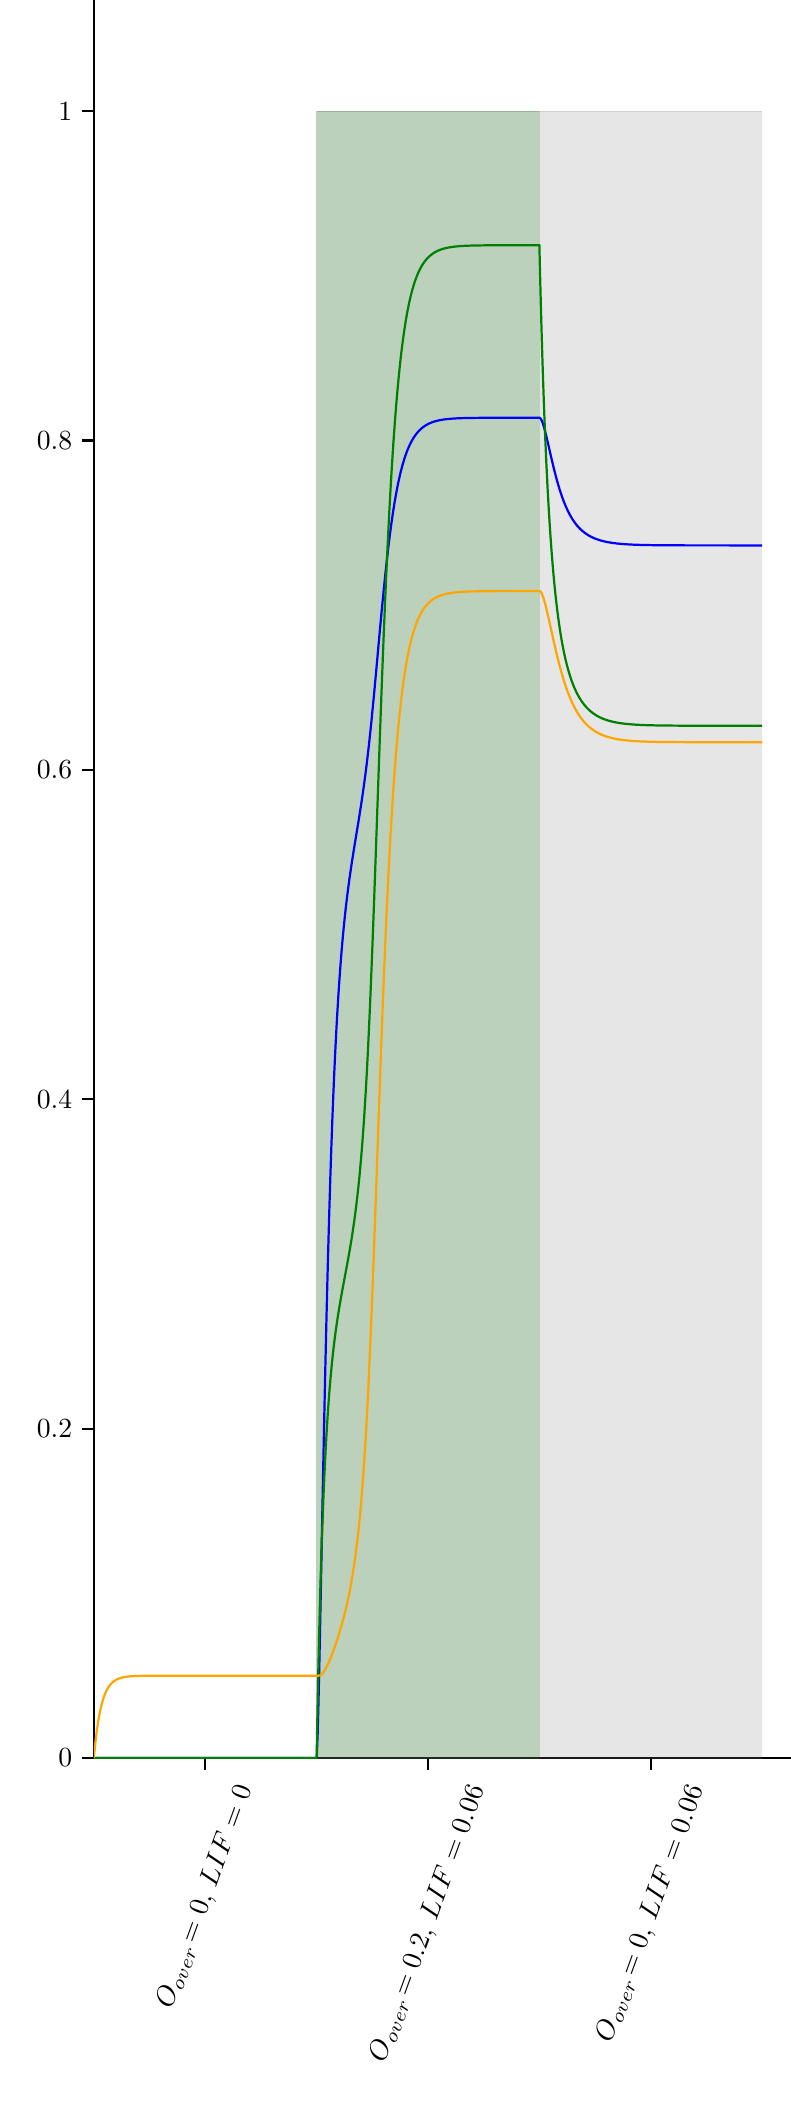
\begin{tikzpicture}[baseline]

\definecolor{darkgray176}{RGB}{176,176,176}
\definecolor{gray}{RGB}{128,128,128}
\definecolor{green}{RGB}{0,128,0}
\definecolor{lightgray204}{RGB}{204,204,204}
\definecolor{orange}{RGB}{255,165,0}

\begin{axis}[
 ytick={0,0.2,0.4,0.6,0.8,1},
 x tick label style = {rotate=70},
 y post scale=3, 
 transpose legend,
legend cell align={left},
legend style={
  fill opacity=0.8,
  draw opacity=1,
  text opacity=1,
  at={(axis cs:5,1.1)},
  anchor=south west,
    legend columns=4,
    /tikz/every even column/.append style={column sep=1.0cm},,
  draw=lightgray204
},
tick align=outside,
tick pos=left,
x grid style={darkgray176},
xmin=0, xmax=90,
xtick style={color=black},
xtick={15,45,75},
xticklabels={
  {\(\displaystyle O_\text{over}\!=0\), \(\displaystyle \text{LIF}=0\)},
  {\(\displaystyle O_\text{over}\!=0.2\), \(\displaystyle \text{LIF}=0.06\)},
  {\(\displaystyle O_\text{over}\!=0\), \(\displaystyle \text{LIF}=0.06\)}
},
y grid style={darkgray176},
ymin=0, ymax=1.05,
ytick style={color=black}
]
\path [draw=green, fill=green, opacity=0.2]
(axis cs:30,0)
--(axis cs:30,1)
--(axis cs:60,1)
--(axis cs:60,0)
--cycle;

\path [draw=gray, fill=gray, opacity=0.2]
(axis cs:30,0)
--(axis cs:30,1)
--(axis cs:90,1)
--(axis cs:90,0)
--cycle;

\addplot [thick, blue]
table {%
0 0
0.0001 0
0.0011 0
0.0111 0
0.1111 0
0.2111 0
0.3111 0
0.4111 0
0.5111 0
0.6111 0
0.7111 0
0.8111 0
0.9111 0
1.0111 0
1.1111 0
1.2111 0
1.3111 0
1.4111 0
1.5111 0
1.6111 0
1.7111 0
1.8111 0
1.9111 0
2.0111 0
2.1111 0
2.2111 0
2.3111 0
2.4111 0
2.5111 0
2.6111 0
2.7111 0
2.8111 0
2.9111 0
3.0111 0
3.1111 0
3.2111 0
3.3111 0
3.4111 0
3.5111 0
3.6111 0
3.7111 0
3.8111 0
3.9111 0
4.0111 0
4.1111 0
4.2111 0
4.3111 0
4.4111 0
4.5111 0
4.6111 0
4.7111 0
4.8111 0
4.9111 0
5.0111 0
5.1111 0
5.2111 0
5.3111 0
5.4111 0
5.5111 0
5.6111 0
5.7111 0
5.8111 0
5.9111 0
6.0111 0
6.1111 0
6.21109999999999 0
6.31109999999999 0
6.41109999999999 0
6.51109999999999 0
6.61109999999999 0
6.71109999999999 0
6.81109999999999 0
6.91109999999999 0
7.01109999999999 0
7.11109999999999 0
7.21109999999999 0
7.31109999999999 0
7.41109999999999 0
7.51109999999999 0
7.61109999999999 0
7.71109999999999 0
7.81109999999999 0
7.91109999999999 0
8.01109999999999 0
8.11109999999999 0
8.21109999999999 0
8.31109999999999 0
8.41109999999999 0
8.51109999999999 0
8.61109999999999 0
8.71109999999999 0
8.81109999999999 0
8.91109999999999 0
9.01109999999998 0
9.11109999999998 0
9.21109999999998 0
9.31109999999998 0
9.41109999999998 0
9.51109999999998 0
9.61109999999998 0
9.71109999999998 0
9.81109999999998 0
9.91109999999998 0
10.0111 0
10.1111 0
10.2111 0
10.3111 0
10.4111 0
10.5111 0
10.6111 0
10.7111 0
10.8111 0
10.9111 0
11.0111 0
11.1111 0
11.2111 0
11.3111 0
11.4111 0
11.5111 0
11.6111 0
11.7111 0
11.8111 0
11.9111 0
12.0111 0
12.1111 0
12.2111 0
12.3111 0
12.4111 0
12.5111 0
12.6111 0
12.7111 0
12.8111 0
12.9111 0
13.0111 0
13.1111 0
13.2111 0
13.3111 0
13.4111 0
13.5111 0
13.6111 0
13.7111 0
13.8111 0
13.9111 0
14.0111 0
14.1111 0
14.2111 0
14.3111 0
14.4111 0
14.5111 0
14.6111 0
14.7111 0
14.8111 0
14.9111 0
15.0111 0
15.1111 0
15.2111 0
15.3111 0
15.4111 0
15.5111 0
15.6111 0
15.7111 0
15.8111 0
15.9111 0
16.0111 0
16.1111 0
16.2111 0
16.3111 0
16.4111 0
16.5111 0
16.6111 0
16.7111 0
16.8111 0
16.9111 0
17.0111 0
17.1111 0
17.2111 0
17.3111 0
17.4111 0
17.5111 0
17.6111 0
17.7111 0
17.8111 0
17.9111 0
18.0111 0
18.1111 0
18.2111 0
18.3111 0
18.4111 0
18.5111 0
18.6111 0
18.7111 0
18.8111 0
18.9111 0
19.0111 0
19.1111 0
19.2111 0
19.3111 0
19.4111 0
19.5111 0
19.6111 0
19.7111 0
19.8111 0
19.9111 0
20.0111 0
20.1111 0
20.2111 0
20.3111 0
20.4111 0
20.5111 0
20.6111 0
20.7111 0
20.8111 0
20.9111 0
21.0111 0
21.1111 0
21.2111 0
21.3111 0
21.4111 0
21.5111 0
21.6111 0
21.7111 0
21.8111 0
21.9111 0
22.0111 0
22.1111 0
22.2111 0
22.3111 0
22.4111000000001 0
22.5111000000001 0
22.6111000000001 0
22.7111000000001 0
22.8111000000001 0
22.9111000000001 0
23.0111000000001 0
23.1111000000001 0
23.2111000000001 0
23.3111000000001 0
23.4111000000001 0
23.5111000000001 0
23.6111000000001 0
23.7111000000001 0
23.8111000000001 0
23.9111000000001 0
24.0111000000001 0
24.1111000000001 0
24.2111000000001 0
24.3111000000001 0
24.4111000000001 0
24.5111000000001 0
24.6111000000001 0
24.7111000000001 0
24.8111000000001 0
24.9111000000001 0
25.0111000000001 0
25.1111000000001 0
25.2111000000001 0
25.3111000000001 0
25.4111000000001 0
25.5111000000001 0
25.6111000000001 0
25.7111000000001 0
25.8111000000001 0
25.9111000000001 0
26.0111000000001 0
26.1111000000001 0
26.2111000000001 0
26.3111000000001 0
26.4111000000001 0
26.5111000000001 0
26.6111000000001 0
26.7111000000001 0
26.8111000000001 0
26.9111000000001 0
27.0111000000001 0
27.1111000000001 0
27.2111000000001 0
27.3111000000001 0
27.4111000000001 0
27.5111000000001 0
27.6111000000001 0
27.7111000000001 0
27.8111000000001 0
27.9111000000001 0
28.0111000000001 0
28.1111000000001 0
28.2111000000001 0
28.3111000000001 0
28.4111000000001 0
28.5111000000001 0
28.6111000000001 0
28.7111000000001 0
28.8111000000001 0
28.9111000000001 0
29.0111000000001 0
29.1111000000001 0
29.2111000000001 0
29.3111000000001 0
29.4111000000002 0
29.5111000000002 0
29.6111000000002 0
29.7111000000002 0
29.8111000000002 0
29.9111000000002 0
30 0
30 0
30.0036741749461 0.000225869163022806
30.0404159244067 0.00305017116226338
30.1404159244067 0.0150897383741094
30.2404159244067 0.0317917489642326
30.3404159244067 0.0515445329130337
30.4404159244067 0.0731998248602922
30.5404159244067 0.0959294065550448
30.6404159244067 0.11913110804805
30.7404159244067 0.142365608652233
30.8404159244067 0.165313017447658
30.9404159244067 0.187742365633434
31.0404159244067 0.209489683068776
31.1404159244067 0.230441913400007
31.2404159244067 0.25052490025637
31.3404159244067 0.269694281308445
31.4404159244067 0.287928504839737
31.5404159244067 0.305223424763949
31.6404159244067 0.321588088055309
31.7404159244067 0.337041434817888
31.8404159244067 0.351609704468139
31.9404159244067 0.365324393153983
32.0404159244067 0.378220644690933
32.1404159244067 0.390335984501434
32.2404159244067 0.401709326270888
32.3404159244067 0.412380196275622
32.4404159244067 0.422388131958556
32.5404159244067 0.431772220279774
32.6404159244067 0.440570748327678
32.7404159244067 0.448820944129408
32.8404159244067 0.456558789903126
32.9404159244067 0.46381889341356
33.0404159244067 0.470634405823184
33.1404159244067 0.477036976624211
33.2404159244067 0.483056738004924
33.3404159244067 0.48872231243571
33.4404159244067 0.494060838423331
33.5404159244067 0.499098010329741
33.6404159244067 0.503858128925607
33.7404159244067 0.508364159981756
33.8404159244067 0.512637798719889
33.9404159244067 0.516699538367945
34.0404159244067 0.520568741411827
34.1404159244067 0.524263712416927
34.2404159244067 0.527801771520304
34.3404159244067 0.531199327875517
34.4404159244067 0.534471952473156
34.5404159244067 0.537634449865597
34.6404159244067 0.540700928397544
34.7404159244067 0.543684868586419
34.8404159244067 0.546599189309421
34.9404159244067 0.549456311436894
35.0404159244067 0.552268218503503
35.1404159244067 0.555046513927997
35.2404159244067 0.557802474177108
35.3404159244067 0.560547097117628
35.4404159244067 0.563291144611994
35.5404159244067 0.566045178187957
35.6404159244067 0.568819586356427
35.7404159244067 0.571624601873134
35.8404159244067 0.574470306956735
35.9404159244067 0.577366624216202
36.0404159244067 0.58032329084473
36.1404159244067 0.583349813562217
36.2404159244067 0.586455401905142
36.3404159244067 0.589648877855827
36.4404159244067 0.592938560560862
36.5404159244067 0.596332126089146
36.6404159244067 0.599836443868052
36.7404159244067 0.603457393594988
36.8404159244067 0.60719966894262
36.9404159244068 0.611066577037763
37.0404159244068 0.615059845159581
37.1404159244068 0.619179447949857
37.2404159244068 0.623423469215287
37.3404159244068 0.627788011766145
37.4404159244068 0.632267166498832
37.5404159244068 0.636853048179744
37.6404159244068 0.641535900503044
37.7404159244068 0.646304267591743
37.8404159244068 0.651145223924213
37.9404159244068 0.656044650392455
38.0404159244068 0.660987541348472
38.1404159244068 0.66595832631391
38.2404159244068 0.670941190472023
38.3404159244068 0.675920379851318
38.4404159244068 0.680880479825764
38.5404159244068 0.685806658736151
38.6404159244068 0.690684871663457
38.7404159244068 0.695502022337239
38.8404159244068 0.700246083635393
38.9404159244068 0.70490617903121
39.0404159244068 0.70947262866259
39.1404159244068 0.713936964489486
39.2404159244068 0.718291919356066
39.3404159244068 0.722531394782739
39.4404159244068 0.72665041207684
39.5404159244068 0.730645050954608
39.6404159244068 0.73451237938114
39.7404159244068 0.73825037781263
39.8404159244068 0.741857860505256
39.9404159244068 0.745334396063198
40.0404159244068 0.748680228950308
40.1404159244068 0.751896203293814
40.2404159244068 0.754983689966734
40.3404159244068 0.757944517647147
40.4404159244068 0.76078090831364
40.5404159244068 0.763495417442326
40.6404159244068 0.766090879016348
40.7404159244068 0.768570355338394
40.8404159244068 0.770937091545083
40.9404159244068 0.773194474654468
41.0404159244068 0.775345996929948
41.1404159244068 0.77739522331184
41.2404159244068 0.779345762648557
41.3404159244068 0.781201242449988
41.4404159244068 0.782965286884029
41.5404159244068 0.784641497741354
41.6404159244068 0.786233438102016
41.7404159244068 0.787744618448882
41.8404159244068 0.789178484986526
41.9404159244068 0.790538409938956
42.0404159244068 0.791827683615096
42.1404159244068 0.793049508046562
42.2404159244068 0.794206992017875
42.3404159244068 0.795303147324309
42.4404159244068 0.796340886107155
42.5404159244068 0.797323019129938
42.6404159244068 0.798252254872186
42.7404159244068 0.799131199329444
42.8404159244068 0.799962356419595
42.9404159244068 0.800748128905935
43.0404159244068 0.801490819757088
43.1404159244068 0.80219263387263
43.2404159244068 0.802855680111317
43.3404159244068 0.803481973566115
43.4404159244068 0.804073438036837
43.5404159244068 0.804631908657186
43.6404159244068 0.805159134638369
43.7404159244068 0.805656782096317
43.8404159244068 0.806126436933881
43.9404159244068 0.806569607753257
44.0404159244069 0.806987728777372
44.1404159244069 0.807382162762058
44.2404159244069 0.807754203883568
44.3404159244069 0.80810508058845
44.4404159244069 0.808435958394924
44.5404159244069 0.808747942636816
44.6404159244069 0.80904208114277
44.7404159244069 0.809319366844935
44.8404159244069 0.809580740312585
44.9404159244069 0.809827092207262
45.0404159244069 0.810059265656996
45.1404159244069 0.810278058548011
45.2404159244069 0.810484225733009
45.3404159244069 0.810678481155799
45.4404159244069 0.810861499892517
45.5404159244069 0.811033920110164
45.6404159244069 0.81119634494354
45.7404159244069 0.811349344291983
45.8404159244069 0.811493456537574
45.9404159244069 0.811629190186668
46.0404159244069 0.811757025436784
46.1404159244069 0.811877415671031
46.2404159244069 0.811990788882309
46.3404159244069 0.812097549029625
46.4404159244069 0.812198077328896
46.5404159244069 0.812292733480632
46.6404159244069 0.8123818568369
46.7404159244069 0.812465767509968
46.8404159244069 0.812544767424999
46.9404159244069 0.812619141319134
47.0404159244069 0.812689157689262
47.1404159244069 0.812755069690724
47.2404159244069 0.812817115989161
47.3404159244069 0.812875521567625
47.4404159244069 0.812930498491037
47.5404159244069 0.812982246629996
47.6404159244069 0.813030954345893
47.7404159244069 0.813076799139187
47.8404159244069 0.813119948262657
47.9404159244069 0.813160559301363
48.0404159244069 0.813198780720989
48.1404159244069 0.813234752386155
48.2404159244069 0.813268606050234
48.3404159244069 0.813300465818153
48.4404159244069 0.813330448583553
48.5404159244069 0.813358664441667
48.6404159244069 0.81338521707919
48.7404159244069 0.813410204142345
48.8404159244069 0.813433717584326
48.9404159244069 0.813455843993203
49.0404159244069 0.813476664901352
49.1404159244069 0.813496257077403
49.2404159244069 0.813514692801665
49.3404159244069 0.81353204012591
49.4404159244069 0.813548363118404
49.5404159244069 0.813563722094962
49.6404159244069 0.813578173836822
49.7404159244069 0.813591771796068
49.8404159244069 0.813604566289277
49.9404159244069 0.813616604680064
50.0404159244069 0.81362793155114
50.1404159244069 0.813638588866466
50.2404159244069 0.813648616124071
50.3404159244069 0.813658050500051
50.4404159244069 0.813666926984251
50.5404159244069 0.813675278508099
50.6404159244069 0.813683136065042
50.7404159244069 0.813690528824001
50.8404159244069 0.813697484236243
50.9404159244069 0.813704028136048
51.040415924407 0.813710184835525
51.140415924407 0.813715977213908
51.240415924407 0.813721426801656
51.340415924407 0.813726553859653
51.440415924407 0.813731377453787
51.540415924407 0.813735915525175
51.640415924407 0.813740184956291
51.740415924407 0.813744201633225
51.840415924407 0.813747980504305
51.940415924407 0.813751535635283
52.040415924407 0.813754880261299
52.140415924407 0.813758026835791
52.240415924407 0.813760987076545
52.340415924407 0.813763772009042
52.440415924407 0.813766392007261
52.540415924407 0.813768856832089
52.640415924407 0.813771175667477
52.740415924407 0.813773357154463
52.840415924407 0.813775409423208
52.940415924407 0.81377734012314
53.040415924407 0.813779156451326
53.140415924407 0.813780865179179
53.240415924407 0.813782472677587
53.340415924407 0.813783984940568
53.440415924407 0.813785407607529
53.540415924407 0.813786745984213
53.640415924407 0.813788005062414
53.740415924407 0.813789189538531
53.840415924407 0.813790303831021
53.940415924407 0.813791352096832
54.040415924407 0.813792338246862
54.140415924407 0.813793265960504
54.240415924407 0.813794138699337
54.340415924407 0.813794959720008
54.440415924407 0.813795732086349
54.540415924407 0.813796458680785
54.640415924407 0.813797142215065
54.740415924407 0.81379778524036
54.840415924407 0.81379839015676
54.940415924407 0.81379895922222
55.040415924407 0.813799494560966
55.140415924407 0.813799998171413
55.240415924407 0.813800471933609
55.340415924407 0.813800917616241
55.440415924407 0.81380133688323
55.540415924407 0.81380173129993
55.640415924407 0.813802102338965
55.740415924407 0.813802451385719
55.840415924407 0.8138027797435
55.940415924407 0.813803088638403
56.040415924407 0.813803379223879
56.140415924407 0.81380365258504
56.240415924407 0.813803909742704
56.340415924407 0.813804151657203
56.440415924407 0.813804379231968
56.540415924407 0.813804593316896
56.640415924407 0.813804794711521
56.740415924407 0.813804984168001
56.840415924407 0.813805162393921
56.940415924407 0.813805330054933
57.040415924407 0.813805487777245
57.140415924407 0.813805636149951
57.240415924407 0.813805775727236
57.340415924407 0.813805907030439
57.440415924407 0.813806030550004
57.540415924407 0.813806146747307
57.640415924407 0.813806256056381
57.740415924407 0.813806358885531
57.840415924407 0.813806455618867
57.940415924407 0.81380654661773
58.040415924407 0.813806632222045
58.1404159244071 0.81380671275159
58.2404159244071 0.813806788507186
58.3404159244071 0.813806859771829
58.4404159244071 0.813806926811736
58.5404159244071 0.813806989877348
58.6404159244071 0.813807049204259
58.7404159244071 0.813807105014098
58.8404159244071 0.813807157515359
58.9404159244071 0.813807206904176
59.0404159244071 0.813807253365057
59.1404159244071 0.813807297071573
59.2404159244071 0.813807338187007
59.3404159244071 0.813807376864961
59.4404159244071 0.813807413249935
59.5404159244071 0.813807447477859
59.6404159244071 0.813807479676609
59.7404159244071 0.81380750996648
59.8404159244071 0.813807538460634
59.9404159244071 0.813807565265526
60 0.813807580475291
60 0.813807580475291
60.1 0.813615369468321
60.2 0.813075804786177
60.3 0.812240126721427
60.4 0.811154076751754
60.5 0.809858388067275
60.6 0.80838924026698
60.7 0.806778680212312
60.8 0.805055010914077
60.9 0.803243150245752
61 0.801364961211804
61.1 0.799439555446268
61.2 0.797483571568961
61.3 0.795511429980515
61.4 0.793535565630387
61.5 0.79156664024263
61.6 0.789613735431816
61.7 0.787684528085886
61.8 0.785785449334119
61.9 0.783921828357269
62 0.782098022233958
62.1 0.780317532953098
62.2 0.778583112657345
62.3 0.776896858117866
62.4 0.77526029537667
62.5 0.773674455429973
62.6 0.772139941764924
62.7 0.77065699050293
62.8 0.76922552384606
62.9 0.767845197468812
63 0.766515442446037
63.1 0.765235502259146
63.2 0.764004465376916
63.3 0.762821293864278
63.4 0.761684848432394
63.5 0.760593910305992
63.6000000000001 0.759547200249363
63.7000000000001 0.758543395060389
63.8000000000001 0.757581141812495
63.9000000000001 0.756659070097254
64.0000000000001 0.755775802495482
64.1000000000001 0.754929963481863
64.2 0.754120186947334
64.3 0.753345122504468
64.4 0.752603440723851
64.5 0.751893837433756
64.6 0.751215037201227
64.7 0.750565796099832
64.8 0.749944903857731
64.9 0.749351185469236
65 0.748783502343632
65.1 0.748240753056533
65.2 0.747721873761459
65.3 0.747225838312496
65.4 0.746751658142814
65.5 0.746298381938343
65.6 0.745865095141074
65.7 0.74545091931209
65.8 0.745055011380608
65.8999999999999 0.744676562801843
65.9999999999999 0.744314798643527
66.0999999999999 0.743968976618165
66.1999999999999 0.743638386075778
66.2999999999999 0.743322346969758
66.3999999999999 0.74302020880662
66.4999999999999 0.742731349588801
66.5999999999999 0.742455174758248
66.6999999999999 0.742191116147255
66.7999999999999 0.741938630941943
66.8999999999999 0.741697200662808
66.9999999999999 0.741466330165938
67.0999999999999 0.741245546667777
67.1999999999999 0.741034398795699
67.2999999999999 0.740832455666105
67.3999999999999 0.740639305991312
67.4999999999999 0.740454557216083
67.5999999999999 0.740277834684357
67.6999999999998 0.740108780836387
67.7999999999998 0.739947054436326
67.8999999999998 0.739792329830043
67.9999999999998 0.739644296232821
68.0999999999998 0.739502657046439
68.1999999999998 0.739367129205025
68.2999999999998 0.739237442548992
68.3999999999998 0.7391133392263
68.4999999999998 0.738994573120207
68.5999999999998 0.738880909302688
68.6999999999998 0.738772123512612
68.7999999999998 0.738668001657811
68.8999999999998 0.738568339340118
68.9999999999998 0.738472941402489
69.0999999999998 0.738381621497314
69.1999999999998 0.738294201675028
69.2999999999998 0.738210511992162
69.3999999999997 0.738130390137991
69.4999999999997 0.738053681078947
69.5999999999997 0.737980236719997
69.6999999999997 0.737909915582211
69.7999999999997 0.737842582495775
69.8999999999997 0.737778108307714
69.9999999999997 0.737716369603637
70.0999999999997 0.737657248442841
70.1999999999997 0.73760063210611
70.2999999999997 0.737546412855627
70.3999999999997 0.737494487706385
70.4999999999997 0.737444758208542
70.5999999999997 0.737397130240195
70.6999999999997 0.737351513810046
70.7999999999997 0.737307822869481
70.8999999999997 0.737265975133595
70.9999999999997 0.737225891910726
71.0999999999997 0.737187497940064
71.1999999999996 0.737150721236952
71.2999999999996 0.73711549294549
71.3999999999996 0.737081747198078
71.4999999999996 0.737049420981561
71.5999999999996 0.737018454009647
71.6999999999996 0.736988788601294
71.7999999999996 0.736960369564757
71.8999999999996 0.736933144087039
71.9999999999996 0.736907061628464
72.0999999999996 0.736882073822126
72.1999999999996 0.736858134377978
72.2999999999996 0.736835198991335
72.3999999999996 0.73681322525557
72.4999999999996 0.736792172578816
72.5999999999996 0.736772002104453
72.6999999999996 0.73675267663523
72.7999999999996 0.736734160560824
72.8999999999996 0.736716419788678
72.9999999999995 0.736699421677965
73.0999999999995 0.736683134976527
73.1999999999995 0.736667529760648
73.2999999999995 0.736652577377522
73.3999999999995 0.736638250390302
73.4999999999995 0.73662452252559
73.5999999999995 0.736611368623273
73.6999999999995 0.736598764588585
73.7999999999995 0.736586687346285
73.8999999999995 0.736575114796873
73.9999999999995 0.736564025774729
74.0999999999995 0.736553400008097
74.1999999999995 0.73654321808083
74.2999999999995 0.736533461395808
74.3999999999995 0.736524112139961
74.4999999999995 0.73651515325082
74.5999999999995 0.736506568384519
74.6999999999994 0.736498341885206
74.7999999999994 0.736490458755766
74.8999999999994 0.736482904629823
74.9999999999994 0.736475665744957
75.0999999999994 0.736468728917072
75.1999999999994 0.736462081515878
75.2999999999994 0.736455711441428
75.3999999999994 0.73644960710166
75.4999999999994 0.736443757390915
75.5999999999994 0.736438151669372
75.6999999999994 0.736432779743361
75.7999999999994 0.73642763184653
75.8999999999994 0.73642269862181
75.9999999999994 0.736417971104149
76.0999999999994 0.736413440703994
76.1999999999994 0.736409099191469
76.2999999999994 0.736404938681226
76.3999999999994 0.736400951617948
76.4999999999993 0.736397130762462
76.5999999999993 0.736393469178449
76.6999999999993 0.736389960219709
76.7999999999993 0.736386597517976
76.8999999999993 0.736383374971243
76.9999999999993 0.736380286732583
77.0999999999993 0.736377327199448
77.1999999999993 0.736374491003408
77.2999999999993 0.736371773000343
77.3999999999993 0.736369168261028
77.4999999999993 0.736366672062135
77.5999999999993 0.736364279877597
77.6999999999993 0.736361987370354
77.7999999999993 0.736359790384429
77.8999999999993 0.736357684937352
77.9999999999993 0.736355667212893
78.0999999999993 0.736353733554111
78.1999999999992 0.736351880456682
78.2999999999992 0.736350104562523
78.3999999999992 0.736348402653668
78.4999999999992 0.736346771646414
78.5999999999992 0.736345208585709
78.6999999999992 0.73634371063977
78.7999999999992 0.736342275094935
78.8999999999992 0.736340899350726
78.9999999999992 0.736339580915121
79.0999999999992 0.736338317400021
79.1999999999992 0.736337106516915
79.2999999999992 0.736335946072715
79.3999999999992 0.736334833965776
79.4999999999992 0.736333768182075
79.5999999999992 0.736332746791555
79.6999999999992 0.736331767944622
79.7999999999992 0.736330829868781
79.8999999999992 0.736329930865425
79.9999999999991 0.736329069306748
80.0999999999991 0.736328243632793
80.1999999999991 0.736327452348618
80.2999999999991 0.736326694021588
80.3999999999991 0.736325967278772
80.4999999999991 0.736325270804457
80.5999999999991 0.736324603337758
80.6999999999991 0.736323963670332
80.7999999999991 0.73632335064419
80.8999999999991 0.736322763149591
80.9999999999991 0.736322200123039
81.0999999999991 0.736321660545347
81.1999999999991 0.736321143439793
81.2999999999991 0.73632064787035
81.3999999999991 0.736320172939989
81.4999999999991 0.736319717789054
81.5999999999991 0.736319281593702
81.6999999999991 0.736318863564414
81.799999999999 0.736318462944559
81.899999999999 0.736318079009029
81.999999999999 0.736317711062924
82.099999999999 0.736317358440287
82.199999999999 0.736317020502908
82.299999999999 0.736316696639159
82.399999999999 0.736316386262892
82.499999999999 0.736316088812373
82.599999999999 0.736315803749268
82.699999999999 0.736315530557666
82.799999999999 0.736315268743146
82.899999999999 0.736315017831882
82.999999999999 0.736314777369782
83.099999999999 0.736314546921669
83.199999999999 0.736314326070491
83.299999999999 0.736314114416569
83.399999999999 0.736313911576868
83.4999999999989 0.736313717184309
83.5999999999989 0.7363135308871
83.6999999999989 0.736313352348102
83.7999999999989 0.736313181244218
83.8999999999989 0.736313017265807
83.9999999999989 0.736312860116125
84.0999999999989 0.736312709510785
84.1999999999989 0.736312565177247
84.2999999999989 0.736312426854319
84.3999999999989 0.73631229429169
84.4999999999989 0.736312167249472
84.5999999999989 0.736312045497767
84.6999999999989 0.736311928816254
84.7999999999989 0.736311816993786
84.8999999999989 0.736311709828009
84.9999999999989 0.736311607124999
85.0999999999989 0.736311508698905
85.1999999999989 0.736311414371617
85.2999999999988 0.736311323972445
85.3999999999988 0.736311237337805
85.4999999999988 0.736311154310925
85.5999999999988 0.736311074741565
85.6999999999988 0.736310998485738
85.7999999999988 0.736310925405457
85.8999999999988 0.736310855368479
85.9999999999988 0.736310788248069
86.0999999999988 0.73631072392277
86.1999999999988 0.736310662276183
86.2999999999988 0.736310603196757
86.3999999999988 0.736310546577586
86.4999999999988 0.736310492316215
86.5999999999988 0.736310440314458
86.6999999999988 0.736310390478216
86.7999999999988 0.736310342717309
86.8999999999988 0.736310296945314
86.9999999999987 0.736310253079405
87.0999999999987 0.736310211040206
87.1999999999987 0.736310170751646
87.2999999999987 0.736310132140824
87.3999999999987 0.736310095137873
87.4999999999987 0.736310059675835
87.5999999999987 0.736310025690543
87.6999999999987 0.736309993120499
87.7999999999987 0.736309961906768
87.8999999999987 0.736309931992868
87.9999999999987 0.736309903324672
88.0999999999987 0.736309875850303
88.1999999999987 0.736309849520047
88.2999999999987 0.736309824286259
88.3999999999987 0.73630980010328
88.4999999999987 0.73630977692735
88.5999999999987 0.736309754716533
88.6999999999987 0.736309733430638
88.7999999999986 0.736309713031148
88.8999999999986 0.736309693481152
88.9999999999986 0.736309674745274
89.0999999999986 0.736309656789611
89.1999999999986 0.736309639581673
89.2999999999986 0.736309623090323
89.3999999999986 0.736309607285719
89.4999999999986 0.736309592139264
89.5999999999986 0.736309577623549
89.6999999999986 0.73630956371231
89.7999999999986 0.736309550380375
89.8999999999986 0.736309537603618
89.9999999999986 0.736309525358922
90 0.736309525358922
};
\addplot [thick, green]
table {%
0 0
0.0001 0
0.0011 0
0.0111 0
0.1111 0
0.2111 0
0.3111 0
0.4111 0
0.5111 0
0.6111 0
0.7111 0
0.8111 0
0.9111 0
1.0111 0
1.1111 0
1.2111 0
1.3111 0
1.4111 0
1.5111 0
1.6111 0
1.7111 0
1.8111 0
1.9111 0
2.0111 0
2.1111 0
2.2111 0
2.3111 0
2.4111 0
2.5111 0
2.6111 0
2.7111 0
2.8111 0
2.9111 0
3.0111 0
3.1111 0
3.2111 0
3.3111 0
3.4111 0
3.5111 0
3.6111 0
3.7111 0
3.8111 0
3.9111 0
4.0111 0
4.1111 0
4.2111 0
4.3111 0
4.4111 0
4.5111 0
4.6111 0
4.7111 0
4.8111 0
4.9111 0
5.0111 0
5.1111 0
5.2111 0
5.3111 0
5.4111 0
5.5111 0
5.6111 0
5.7111 0
5.8111 0
5.9111 0
6.0111 0
6.1111 0
6.21109999999999 0
6.31109999999999 0
6.41109999999999 0
6.51109999999999 0
6.61109999999999 0
6.71109999999999 0
6.81109999999999 0
6.91109999999999 0
7.01109999999999 0
7.11109999999999 0
7.21109999999999 0
7.31109999999999 0
7.41109999999999 0
7.51109999999999 0
7.61109999999999 0
7.71109999999999 0
7.81109999999999 0
7.91109999999999 0
8.01109999999999 0
8.11109999999999 0
8.21109999999999 0
8.31109999999999 0
8.41109999999999 0
8.51109999999999 0
8.61109999999999 0
8.71109999999999 0
8.81109999999999 0
8.91109999999999 0
9.01109999999998 0
9.11109999999998 0
9.21109999999998 0
9.31109999999998 0
9.41109999999998 0
9.51109999999998 0
9.61109999999998 0
9.71109999999998 0
9.81109999999998 0
9.91109999999998 0
10.0111 0
10.1111 0
10.2111 0
10.3111 0
10.4111 0
10.5111 0
10.6111 0
10.7111 0
10.8111 0
10.9111 0
11.0111 0
11.1111 0
11.2111 0
11.3111 0
11.4111 0
11.5111 0
11.6111 0
11.7111 0
11.8111 0
11.9111 0
12.0111 0
12.1111 0
12.2111 0
12.3111 0
12.4111 0
12.5111 0
12.6111 0
12.7111 0
12.8111 0
12.9111 0
13.0111 0
13.1111 0
13.2111 0
13.3111 0
13.4111 0
13.5111 0
13.6111 0
13.7111 0
13.8111 0
13.9111 0
14.0111 0
14.1111 0
14.2111 0
14.3111 0
14.4111 0
14.5111 0
14.6111 0
14.7111 0
14.8111 0
14.9111 0
15.0111 0
15.1111 0
15.2111 0
15.3111 0
15.4111 0
15.5111 0
15.6111 0
15.7111 0
15.8111 0
15.9111 0
16.0111 0
16.1111 0
16.2111 0
16.3111 0
16.4111 0
16.5111 0
16.6111 0
16.7111 0
16.8111 0
16.9111 0
17.0111 0
17.1111 0
17.2111 0
17.3111 0
17.4111 0
17.5111 0
17.6111 0
17.7111 0
17.8111 0
17.9111 0
18.0111 0
18.1111 0
18.2111 0
18.3111 0
18.4111 0
18.5111 0
18.6111 0
18.7111 0
18.8111 0
18.9111 0
19.0111 0
19.1111 0
19.2111 0
19.3111 0
19.4111 0
19.5111 0
19.6111 0
19.7111 0
19.8111 0
19.9111 0
20.0111 0
20.1111 0
20.2111 0
20.3111 0
20.4111 0
20.5111 0
20.6111 0
20.7111 0
20.8111 0
20.9111 0
21.0111 0
21.1111 0
21.2111 0
21.3111 0
21.4111 0
21.5111 0
21.6111 0
21.7111 0
21.8111 0
21.9111 0
22.0111 0
22.1111 0
22.2111 0
22.3111 0
22.4111000000001 0
22.5111000000001 0
22.6111000000001 0
22.7111000000001 0
22.8111000000001 0
22.9111000000001 0
23.0111000000001 0
23.1111000000001 0
23.2111000000001 0
23.3111000000001 0
23.4111000000001 0
23.5111000000001 0
23.6111000000001 0
23.7111000000001 0
23.8111000000001 0
23.9111000000001 0
24.0111000000001 0
24.1111000000001 0
24.2111000000001 0
24.3111000000001 0
24.4111000000001 0
24.5111000000001 0
24.6111000000001 0
24.7111000000001 0
24.8111000000001 0
24.9111000000001 0
25.0111000000001 0
25.1111000000001 0
25.2111000000001 0
25.3111000000001 0
25.4111000000001 0
25.5111000000001 0
25.6111000000001 0
25.7111000000001 0
25.8111000000001 0
25.9111000000001 0
26.0111000000001 0
26.1111000000001 0
26.2111000000001 0
26.3111000000001 0
26.4111000000001 0
26.5111000000001 0
26.6111000000001 0
26.7111000000001 0
26.8111000000001 0
26.9111000000001 0
27.0111000000001 0
27.1111000000001 0
27.2111000000001 0
27.3111000000001 0
27.4111000000001 0
27.5111000000001 0
27.6111000000001 0
27.7111000000001 0
27.8111000000001 0
27.9111000000001 0
28.0111000000001 0
28.1111000000001 0
28.2111000000001 0
28.3111000000001 0
28.4111000000001 0
28.5111000000001 0
28.6111000000001 0
28.7111000000001 0
28.8111000000001 0
28.9111000000001 0
29.0111000000001 0
29.1111000000001 0
29.2111000000001 0
29.3111000000001 0
29.4111000000002 0
29.5111000000002 0
29.6111000000002 0
29.7111000000002 0
29.8111000000002 0
29.9111000000002 0
30 0
30 0
30.0036741749461 0.00095353269073373
30.0404159244067 0.0102986321711862
30.1404159244067 0.0340626039090136
30.2404159244067 0.055579659039436
30.3404159244067 0.075091014232352
30.4404159244067 0.092819756647362
30.5404159244067 0.108962585900209
30.6404159244067 0.12368862988709
30.7404159244067 0.137142994026155
30.8404159244067 0.149451490606323
30.9404159244067 0.160724725650666
31.0404159244067 0.171061127518713
31.1404159244067 0.180549077757416
31.2404159244067 0.189268414918964
31.3404159244067 0.197291533607424
31.4404159244067 0.204684228616161
31.5404159244067 0.211506376980704
31.6404159244067 0.217812513247727
31.7404159244067 0.223652330459321
31.8404159244067 0.22907112604122
31.9404159244067 0.2341102041769
32.0404159244067 0.238807241949516
32.1404159244067 0.243196624112859
32.2404159244067 0.247309749986253
32.3404159244067 0.251175315188591
32.4404159244067 0.254819570470237
32.5404159244067 0.258266559621802
32.6404159244067 0.261538338254794
32.7404159244067 0.264655175116449
32.8404159244067 0.267635737496103
32.9404159244067 0.270497262190618
33.0404159244067 0.273255713415572
33.1404159244067 0.275925928974073
33.2404159244067 0.278521755925025
33.3404159244067 0.281056176926963
33.4404159244067 0.283541428372086
33.5404159244067 0.2859891113677
33.6404159244067 0.288410296568765
33.7404159244067 0.290815623815047
33.8404159244067 0.293215397478768
33.9404159244067 0.29561967838235
34.0404159244067 0.298038373099108
34.1404159244067 0.300481321400141
34.2404159244067 0.302958382554935
34.3404159244067 0.30547952112702
34.4404159244067 0.30805489282381
34.5404159244067 0.310694930854144
34.6404159244067 0.313410433108891
34.7404159244067 0.316212650297408
34.8404159244067 0.31911337493132
34.9404159244067 0.322125030729205
35.0404159244067 0.325260761600395
35.1404159244067 0.328534518829238
35.2404159244067 0.331961144396245
35.3404159244067 0.335556447512979
35.4404159244067 0.339337270389149
35.5404159244067 0.343321537977939
35.6404159244067 0.347528284960591
35.7404159244067 0.351977651564502
35.8404159244067 0.356690838037014
35.9404159244067 0.361690005861213
36.0404159244067 0.366998112329005
36.1404159244067 0.372638664214175
36.2404159244067 0.378635376460333
36.3404159244067 0.385011723558742
36.4404159244067 0.391790375225112
36.5404159244067 0.398992514615401
36.6404159244067 0.406637046943886
36.7404159244067 0.414739718839143
36.8404159244067 0.423312183300183
36.9404159244068 0.43236106010706
37.0404159244068 0.441887054646365
37.1404159244068 0.451884206507002
37.2404159244068 0.462339340156515
37.3404159244068 0.47323178164839
37.4404159244068 0.484533387342924
37.5404159244068 0.496208904750375
37.6404159244068 0.508216655390129
37.7404159244068 0.520509499710953
37.8404159244068 0.533036019367204
37.9404159244068 0.545741836111754
38.0404159244068 0.558570980970939
38.1404159244068 0.571467231845776
38.2404159244068 0.584375350167164
38.3404159244068 0.59724216468635
38.4404159244068 0.610017469717343
38.5404159244068 0.622654723463313
38.6404159244068 0.635111547590902
38.7404159244068 0.647350041008721
38.8404159244068 0.65933692867675
38.9404159244068 0.671043570582247
39.0404159244068 0.682445857426044
39.1404159244068 0.693524018832578
39.2404159244068 0.704262367753104
39.3404159244068 0.714649001787514
39.4404159244068 0.724675478878094
39.5404159244068 0.734336481561429
39.6404159244068 0.74362948091626
39.7404159244068 0.75255440863477
39.8404159244068 0.76111334332381
39.9404159244068 0.769310215215822
40.0404159244068 0.777150531913319
40.1404159244068 0.784641126566476
40.2404159244068 0.791789928945164
40.3404159244068 0.798605759168247
40.4404159244068 0.805098143350573
40.5404159244068 0.811277150082778
40.6404159244068 0.817153246437155
40.7404159244068 0.822737172065989
40.8404159244068 0.828039829903699
40.9404159244068 0.833072191981889
41.0404159244068 0.837845218902069
41.1404159244068 0.84236979157263
41.2404159244068 0.846656653895446
41.3404159244068 0.850716365176501
41.4404159244068 0.854559261128868
41.5404159244068 0.858195422431537
41.6404159244068 0.861634649901213
41.7404159244068 0.864886445424438
41.8404159244068 0.867959997882987
41.9404159244068 0.870864173385674
42.0404159244068 0.873607509194094
42.1404159244068 0.876198210798257
42.2404159244068 0.878644151660636
42.3404159244068 0.880952875203947
42.4404159244068 0.883131598669369
42.5404159244068 0.885187218518157
42.6404159244068 0.887126317091058
42.7404159244068 0.88895517027699
42.8404159244068 0.890679755975465
42.9404159244068 0.892305763166537
43.0404159244068 0.893838601428039
43.1404159244068 0.895283410762801
43.2404159244068 0.89664507161878
43.3404159244068 0.897928215002804
43.4404159244068 0.89913723260421
43.5404159244068 0.90027628685834
43.6404159244068 0.901349320891721
43.7404159244068 0.902360068301144
43.8404159244068 0.903312062727881
43.9404159244068 0.904208647196012
44.0404159244069 0.905052983190635
44.1404159244069 0.905848059457447
44.2404159244069 0.906596700510211
44.3404159244069 0.90730157483679
44.4404159244069 0.907965202798096
44.5404159244069 0.908589964217282
44.6404159244069 0.9091781056591
44.7404159244069 0.909731747401472
44.8404159244069 0.910252890103066
44.9404159244069 0.910743421172136
45.0404159244069 0.911205120843047
45.1404159244069 0.911639667967827
45.2404159244069 0.912048645530816
45.3404159244069 0.912433545895038
45.4404159244069 0.912795775789303
45.5404159244069 0.913136661045335
45.6404159244069 0.913457451094354
45.7404159244069 0.913759323232639
45.8404159244069 0.914043386665577
45.9404159244069 0.914310686339609
46.0404159244069 0.914562206571405
46.1404159244069 0.914798874483387
46.2404159244069 0.915021563254549
46.3404159244069 0.91523109519526
46.4404159244069 0.915428244654525
46.5404159244069 0.915613740767864
46.6404159244069 0.915788270053739
46.7404159244069 0.915952478866131
46.8404159244069 0.916106975710599
46.9404159244069 0.916252333430857
47.0404159244069 0.916389091272619
47.1404159244069 0.916517756831152
47.2404159244069 0.916638807888714
47.3404159244069 0.916752694147771
47.4404159244069 0.916859838865601
47.5404159244069 0.916960640395628
47.6404159244069 0.917055473640603
47.7404159244069 0.917144691422443
47.8404159244069 0.91722862577335
47.9404159244069 0.91730758915257
48.0404159244069 0.917381875592939
48.1404159244069 0.917451761781144
48.2404159244069 0.917517508075429
48.3404159244069 0.917579359464274
48.4404159244069 0.917637546469382
48.5404159244069 0.917692285996147
48.6404159244069 0.917743782134583
48.7404159244069 0.917792226913557
48.8404159244069 0.917837801010981
48.9404159244069 0.91788067442251
49.0404159244069 0.917921007091116
49.1404159244069 0.917958949499807
49.2404159244069 0.917994643229611
49.3404159244069 0.918028221484832
49.4404159244069 0.918059809587482
49.5404159244069 0.91808952544268
49.6404159244069 0.918117479976689
49.7404159244069 0.918143777549204
49.8404159244069 0.918168516341375
49.9404159244069 0.918191788720996
50.0404159244069 0.918213681586176
50.1404159244069 0.918234276688767
50.2404159244069 0.918253650938722
50.3404159244069 0.918271876690504
50.4404159244069 0.918289022012599
50.5404159244069 0.918305150941127
50.6404159244069 0.918320323718472
50.7404159244069 0.918334597017832
50.8404159244069 0.918348024154494
50.9404159244069 0.918360655284633
51.040415924407 0.918372537592358
51.140415924407 0.918383715465705
51.240415924407 0.918394230662219
51.340415924407 0.91840412246475
51.440415924407 0.918413427828025
51.540415924407 0.918422181516563
51.640415924407 0.918430416234413
51.740415924407 0.918438162747227
51.840415924407 0.918445449997103
51.940415924407 0.91845230521063
52.040415924407 0.918458754000539
52.140415924407 0.918464820461332
52.240415924407 0.918470527259252
52.340415924407 0.918475895716921
52.440415924407 0.918480945892971
52.540415924407 0.918485696656952
52.640415924407 0.918490165759808
52.740415924407 0.918494369900178
52.840415924407 0.918498324786762
52.940415924407 0.918502045197002
53.040415924407 0.918505545032278
53.140415924407 0.918508837369843
53.240415924407 0.918511934511665
53.340415924407 0.918514848030395
53.440415924407 0.91851758881259
53.540415924407 0.918520167099392
53.640415924407 0.918522592524785
53.740415924407 0.918524874151588
53.840415924407 0.918527020505318
53.940415924407 0.918529039606038
54.040415924407 0.918530938998328
54.140415924407 0.918532725779467
54.240415924407 0.918534406625957
54.340415924407 0.918535987818465
54.440415924407 0.918537475265291
54.540415924407 0.918538874524446
54.640415924407 0.918540190824417
54.740415924407 0.918541429083703
54.840415924407 0.918542593929197
54.940415924407 0.918543689713469
55.040415924407 0.918544720531035
55.140415924407 0.918545690233653
55.240415924407 0.918546602444717
55.340415924407 0.918547460572795
55.440415924407 0.918548267824368
55.540415924407 0.918549027215808
55.640415924407 0.918549741584652
55.740415924407 0.918550413600205
55.840415924407 0.918551045773512
55.940415924407 0.91855164046674
56.040415924407 0.918552199902011
56.140415924407 0.918552726169699
56.240415924407 0.918553221236241
56.340415924407 0.91855368695149
56.440415924407 0.918554125055623
56.540415924407 0.918554537185645
56.640415924407 0.918554924881507
56.740415924407 0.918555289591856
56.840415924407 0.918555632679453
56.940415924407 0.918555955426265
57.040415924407 0.91855625903825
57.140415924407 0.918556544649869
57.240415924407 0.918556813328322
57.340415924407 0.918557066077538
57.440415924407 0.918557303841925
57.540415924407 0.918557527509896
57.640415924407 0.918557737917195
57.740415924407 0.918557935850015
57.840415924407 0.918558122047938
57.940415924407 0.918558297206697
58.040415924407 0.918558461980775
58.1404159244071 0.918558616985856
58.2404159244071 0.918558762801117
58.3404159244071 0.918558899971401
58.4404159244071 0.918559029009245
58.5404159244071 0.9185591503968
58.6404159244071 0.918559264587633
58.7404159244071 0.918559372008417
58.8404159244071 0.918559473060532
58.9404159244071 0.918559568121558
59.0404159244071 0.918559657546692
59.1404159244071 0.918559741670069
59.2404159244071 0.918559820806016
59.3404159244071 0.918559895250225
59.4404159244071 0.918559965280856
59.5404159244071 0.918560031159577
59.6404159244071 0.918560093132544
59.7404159244071 0.918560151431317
59.8404159244071 0.91856020627373
59.9404159244071 0.9185602578647
60 0.918560287138643
60 0.918560287138643
60.1 0.899358347922895
60.2 0.881655707514935
60.3 0.865318183009611
60.4 0.850224872751453
60.5 0.836266732680988
60.6 0.823345316027206
60.7 0.811371656519244
60.8 0.800265277807189
60.9 0.789953313962931
61 0.780369727826962
61.1 0.771454615616421
61.2 0.763153587647184
61.3 0.755417216276707
61.4 0.748200543268725
61.5 0.74146263973644
61.6 0.735166212655376
61.7 0.729277252666076
61.8 0.723764718523799
61.9 0.718600254109065
62 0.71375793439958
62.1 0.709214037229754
62.2 0.704946838036483
62.3 0.700936425115974
62.4 0.697164533202144
62.5 0.693614393427646
62.6 0.690270597948484
62.7 0.687118977706337
62.8 0.684146491972598
62.9 0.681341128467708
63 0.678691812981192
63.1 0.676188327534156
63.2 0.673821236228839
63.3 0.671581818020744
63.4 0.669462005729517
63.5 0.667454330676174
63.6000000000001 0.665551872397833
63.7000000000001 0.663748212947519
63.8000000000001 0.662037395336948
63.9000000000001 0.660413885724954
64.0000000000001 0.658872538994291
64.1000000000001 0.657408567395223
64.2 0.656017511966327
64.3 0.654695216471522
64.4 0.653437803618
64.5 0.652241653342726
64.6 0.651103382975843
64.7 0.650019829107848
64.8 0.648988031004097
64.9 0.648005215425205
65 0.647068782725413
65.1 0.64617629411316
65.2 0.645325459969084
65.3 0.644514129126552
65.4 0.643740279028744
65.5 0.643002006684397
65.6 0.642297520351557
65.7 0.641625131885288
65.8 0.64098324969121
65.8999999999999 0.640370372232123
65.9999999999999 0.639785082039814
66.0999999999999 0.639226040188566
66.1999999999999 0.63869198119083
66.2999999999999 0.638181708279156
66.3999999999999 0.637694089041712
66.4999999999999 0.637228051381694
66.5999999999999 0.636782579773586
66.6999999999999 0.63635671179168
66.7999999999999 0.635949534888426
66.8999999999999 0.635560183402226
66.9999999999999 0.63518783577604
67.0999999999999 0.634831711969856
67.1999999999999 0.634491071051543
67.2999999999999 0.634165208951961
67.3999999999999 0.633853456371429
67.4999999999999 0.633555176825777
67.5999999999999 0.633269764821199
67.6999999999998 0.632996644148076
67.7999999999998 0.632735266284738
67.8999999999998 0.632485108902928
67.9999999999998 0.63224567446741
68.0999999999998 0.632016488922784
68.1999999999998 0.631797100461166
68.2999999999998 0.631587078364896
68.3999999999998 0.631386011918925
68.4999999999998 0.631193509387951
68.5999999999998 0.631009197053798
68.6999999999998 0.630832718308858
68.7999999999998 0.630663732801771
68.8999999999998 0.630501915631815
68.9999999999998 0.630346956588742
69.0999999999998 0.630198559435061
69.1999999999998 0.63005644122799
69.2999999999998 0.629920331678515
69.3999999999997 0.629789972545181
69.4999999999997 0.629665117060422
69.5999999999997 0.6295455293874
69.6999999999997 0.629430984105455
69.7999999999997 0.629321265722439
69.8999999999997 0.629216168212285
69.9999999999997 0.629115494576325
70.0999999999997 0.629019056426937
70.1999999999997 0.628926673592222
70.2999999999997 0.628838173740495
70.3999999999997 0.628753392023455
70.4999999999997 0.628672170736975
70.5999999999997 0.628594358998524
70.6999999999997 0.628519812440298
70.7999999999997 0.628448392917199
70.8999999999997 0.628379968228851
70.9999999999997 0.6283144118549
71.0999999999997 0.628251602702881
71.1999999999996 0.628191424868
71.2999999999996 0.628133767404191
71.3999999999996 0.628078524105877
71.4999999999996 0.628025593299867
71.5999999999996 0.62797487764689
71.6999999999996 0.627926283952255
71.7999999999996 0.627879722985201
71.8999999999996 0.627835109306483
71.9999999999996 0.627792361103802
72.0999999999996 0.627751400034674
72.1999999999996 0.627712151076399
72.2999999999996 0.627674542382764
72.3999999999996 0.627638505147161
72.4999999999996 0.627603973471821
72.5999999999996 0.62757088424286
72.6999999999996 0.627539177010873
72.7999999999996 0.627508793876798
72.8999999999996 0.627479679382829
72.9999999999995 0.627451780408115
73.0999999999995 0.627425046069039
73.1999999999995 0.627399427623867
73.2999999999995 0.627374878381548
73.3999999999995 0.627351353614502
73.4999999999995 0.627328810475191
73.5999999999995 0.627307207916314
73.6999999999995 0.627286506614455
73.7999999999995 0.627266668897036
73.8999999999995 0.627247658672416
73.9999999999995 0.627229441363012
74.0999999999995 0.627211983841285
74.1999999999995 0.627195254368483
74.2999999999995 0.627179222536011
74.3999999999995 0.627163859209304
74.4999999999995 0.627149136474115
74.5999999999995 0.627135027585083
74.6999999999994 0.627121506916505
74.7999999999994 0.627108549915204
74.8999999999994 0.6270961330554
74.9999999999994 0.627084233795505
75.0999999999994 0.627072830536753
75.1999999999994 0.627061902583583
75.2999999999994 0.627051430105705
75.3999999999994 0.627041394101776
75.4999999999994 0.627031776364605
75.5999999999994 0.627022559447842
75.6999999999994 0.627013726634066
75.7999999999994 0.627005261904224
75.8999999999994 0.626997149908365
75.9999999999994 0.626989375937601
76.0999999999994 0.626981925897256
76.1999999999994 0.626974786281143
76.2999999999994 0.626967944146931
76.3999999999994 0.626961387092537
76.4999999999993 0.626955103233524
76.5999999999993 0.626949081181444
76.6999999999993 0.626943310023089
76.7999999999993 0.626937779300618
76.8999999999993 0.626932478992519
76.9999999999993 0.626927399495365
77.0999999999993 0.626922531606342
77.1999999999993 0.626917866506507
77.2999999999993 0.626913395744748
77.3999999999993 0.626909111222419
77.4999999999993 0.626905005178613
77.5999999999993 0.62690107017606
77.6999999999993 0.626897299087611
77.7999999999993 0.62689368508329
77.8999999999993 0.626890221617884
77.9999999999993 0.626886902419059
78.0999999999993 0.626883721475968
78.1999999999992 0.62688067302834
78.2999999999992 0.626877751556018
78.3999999999992 0.626874951768946
78.4999999999992 0.626872268597565
78.5999999999992 0.626869697183611
78.6999999999992 0.626867232871306
78.7999999999992 0.626864871198909
78.8999999999992 0.626862607890621
78.9999999999992 0.626860438848832
79.0999999999992 0.626858360146689
79.1999999999992 0.626856368020976
79.2999999999992 0.626854458865287
79.3999999999992 0.626852629223493
79.4999999999992 0.626850875783471
79.5999999999992 0.626849195371103
79.6999999999992 0.626847584944523
79.7999999999992 0.626846041588602
79.8999999999992 0.626844562509664
79.9999999999991 0.626843145030427
80.0999999999991 0.626841786585147
80.1999999999991 0.626840484714974
80.2999999999991 0.626839237063491
80.3999999999991 0.626838041372449
80.4999999999991 0.626836895477676
80.5999999999991 0.626835797305153
80.6999999999991 0.62683474486726
80.7999999999991 0.626833736259175
80.8999999999991 0.626832769655422
80.9999999999991 0.626831843306567
81.0999999999991 0.626830955536049
81.1999999999991 0.626830104737144
81.2999999999991 0.626829289370051
81.3999999999991 0.626828507959111
81.4999999999991 0.626827759090127
81.5999999999991 0.626827041407811
81.6999999999991 0.626826353613322
81.799999999999 0.626825694461919
81.899999999999 0.626825062760708
81.999999999999 0.626824457366477
82.099999999999 0.626823877183633
82.199999999999 0.626823321162211
82.299999999999 0.62682278829598
82.399999999999 0.626822277620616
82.499999999999 0.626821788211962
82.599999999999 0.626821319184346
82.699999999999 0.626820869688988
82.799999999999 0.626820438912456
82.899999999999 0.626820026075196
82.999999999999 0.626819630430122
83.099999999999 0.626819251261261
83.199999999999 0.626818887882462
83.299999999999 0.626818539636145
83.399999999999 0.626818205892121
83.4999999999989 0.626817886046444
83.5999999999989 0.626817579520322
83.6999999999989 0.626817285759067
83.7999999999989 0.626817004231091
83.8999999999989 0.626816734426947
83.9999999999989 0.626816475858401
84.0999999999989 0.626816228057555
84.1999999999989 0.626815990575997
84.2999999999989 0.626815762983987
84.3999999999989 0.626815544869684
84.4999999999989 0.626815335838399
84.5999999999989 0.626815135511876
84.6999999999989 0.626814943527616
84.7999999999989 0.626814759538214
84.8999999999989 0.626814583210733
84.9999999999989 0.626814414226102
85.0999999999989 0.626814252278537
85.1999999999989 0.626814097074988
85.2999999999988 0.626813948334609
85.3999999999988 0.626813805788251
85.4999999999988 0.626813669177972
85.5999999999988 0.626813538256573
85.6999999999988 0.626813412787149
85.7999999999988 0.62681329254266
85.8999999999988 0.626813177305522
85.9999999999988 0.626813066867212
86.0999999999988 0.62681296102789
86.1999999999988 0.626812859596039
86.2999999999988 0.626812762388117
86.3999999999988 0.626812669228225
86.4999999999988 0.626812579947791
86.5999999999988 0.626812494385261
86.6999999999988 0.626812412385809
86.7999999999988 0.626812333801058
86.8999999999988 0.626812258488808
86.9999999999987 0.626812186312782
87.0999999999987 0.626812117142377
87.1999999999987 0.626812050852431
87.2999999999987 0.626811987322991
87.3999999999987 0.626811926439102
87.4999999999987 0.626811868090595
87.5999999999987 0.626811812171889
87.6999999999987 0.626811758581799
87.7999999999987 0.626811707223354
87.8999999999987 0.626811658003623
87.9999999999987 0.626811610833542
88.0999999999987 0.626811565627759
88.1999999999987 0.626811522304473
88.2999999999987 0.626811480785293
88.3999999999987 0.626811440995089
88.4999999999987 0.626811402861862
88.5999999999987 0.626811366316611
88.6999999999987 0.626811331293207
88.7999999999986 0.626811297728277
88.8999999999986 0.626811265561085
88.9999999999986 0.626811234733426
89.0999999999986 0.626811205189517
89.1999999999986 0.626811176875899
89.2999999999986 0.62681114974134
89.3999999999986 0.62681112373674
89.4999999999986 0.626811098815044
89.5999999999986 0.626811074931157
89.6999999999986 0.626811052041862
89.7999999999986 0.62681103010574
89.8999999999986 0.626811009083101
89.9999999999986 0.626810988935902
90 0.626810988935902
};
\addplot [thick, orange]
table {%
0 0
0.0001 4.99975000833312e-06
0.0011 5.49697610886171e-05
0.0111 0.0005519311153686
0.1111 0.0052575370088613
0.2111 0.00951534529722334
0.3111 0.0133679695566231
0.4111 0.0168539681453068
0.5111 0.020008230108605
0.6111 0.0228623243602227
0.7111 0.0254448156345365
0.8111 0.027781550372055
0.9111 0.0298959153992811
1.0111 0.0318090719919305
1.1111 0.0335401676640909
1.2111 0.0351065278029765
1.3111 0.036523829067226
1.4111 0.0378062562841701
1.5111 0.0389666444163501
1.6111 0.0400166070181366
1.7111 0.0409666524680836
1.8111 0.041826289140313
1.9111 0.0426041205675177
2.0111 0.0433079315480081
2.1111 0.0439447660585897
2.2111 0.0445209977530499
2.3111 0.0450423937518271
2.4111 0.0455141723612901
2.5111 0.0459410553003014
2.6111 0.046327314956767
2.7111 0.0466768171471296
2.8111 0.0469930598067591
2.9111 0.0472792079984652
3.0111 0.0475381255895092
3.1111 0.0477724039141506
3.2111 0.0479843877085906
3.3111 0.0481761985778802
3.4111 0.0483497562296565
3.5111 0.0485067976872217
3.6111 0.0486488946742563
3.7111 0.0487774693451577
3.8111 0.0488938085184391
3.9111 0.0489990765556421
4.0111 0.0490943270146579
4.1111 0.0491805131940888
4.2111 0.0492584976741811
4.3111 0.0493290609498179
4.4111 0.0493929092419742
4.5111 0.0494506815658139
4.6111 0.0495029561261681
4.7111 0.0495502561044036
4.8111 0.0495930548945974
4.9111 0.0496317808414241
5.0111 0.0496668215271733
5.1111 0.0496985276508032
5.2111 0.0497272165378539
5.3111 0.0497531753163477
5.4111 0.0497766637904631
5.5111 0.0497979170407423
5.6111 0.0498171477768561
5.7111 0.049834548466474
5.8111 0.049850293261545
5.9111 0.0498645397412693
6.0111 0.0498774304892033
6.1111 0.0498890945202844
6.21109999999999 0.0498996485720551
6.31109999999999 0.0499091982730123
6.41109999999999 0.0499178391997722
6.51109999999999 0.0499256578336337
6.61109999999999 0.0499327324261118
6.71109999999999 0.0499391337821054
6.81109999999999 0.0499449259685366
6.91109999999999 0.0499501669555534
7.01109999999999 0.0499549091967153
7.11109999999999 0.0499592001539653
7.21109999999999 0.0499630827726455
7.31109999999999 0.0499665959113086
7.41109999999999 0.0499697747306267
7.51109999999999 0.0499726510452918
7.61109999999999 0.0499752536424277
7.71109999999999 0.0499776085697011
7.81109999999999 0.0499797393960156
7.91109999999999 0.0499816674473969
8.01109999999999 0.0499834120204311
8.11109999999999 0.0499849905753915
8.21109999999999 0.0499864189109866
8.31109999999999 0.049987711322479
8.41109999999999 0.0499888807447571
8.51109999999999 0.0499899388817923
8.61109999999999 0.0499908963237754
8.71109999999999 0.0499917626531076
8.81109999999999 0.0499925465403039
8.91109999999999 0.049993255830771
9.01109999999998 0.049993897623326
9.11109999999998 0.0499944783412446
9.21109999999998 0.0499950037965468
9.31109999999998 0.049995479248166
9.41109999999998 0.0499959094545816
9.51109999999998 0.049996298721444
9.61109999999998 0.0499966509446669
9.71109999999998 0.0499969696494185
9.81109999999998 0.0499972580254032
9.91109999999998 0.0499975189587847
10.0111 0.049997755061072
10.1111 0.049997968695256
10.2111 0.0499981619994596
10.3111 0.0499983369083362
10.4111 0.0499984951724324
10.5111 0.0499986383757087
10.6111 0.0499987679513915
10.7111 0.0499988851963179
10.8111 0.0499989912839143
10.9111 0.0499990872759412
11.0111 0.049999174133119
11.1111 0.0499992527247435
11.2111 0.0499993238373861
11.3111 0.0499993881827661
11.4111 0.0499994464048736
11.5111 0.049999499086415
11.6111 0.0499995467546449
11.7111 0.0499995898866431
11.8111 0.0499996289140889
11.9111 0.0499996642275822
12.0111 0.0499996961805523
12.1111 0.0499997250927953
12.2111 0.0499997512536747
12.3111 0.0499997749250171
12.4111 0.0499997963437336
12.5111 0.0499998157241897
12.6111 0.0499998332603515
12.7111 0.0499998491277269
12.8111 0.0499998634851219
12.9111 0.0499998764762302
13.0111 0.049999888231071
13.1111 0.0499998988672909
13.2111 0.0499999084913405
13.3111 0.0499999171995408
13.4111 0.0499999250790463
13.5111 0.0499999322087177
13.6111 0.0499999386599111
13.7111 0.0499999444971923
13.8111 0.0499999497789828
13.9111 0.0499999545581444
14.0111 0.0499999588825087
14.1111 0.0499999627953554
14.2111 0.0499999663358454
14.3111 0.0499999695394132
14.4111 0.0499999724381213
14.5111 0.0499999750609809
14.6111 0.0499999774342423
14.7111 0.0499999795816581
14.8111 0.0499999815247202
14.9111 0.0499999832828755
15.0111 0.0499999848737202
15.1111 0.0499999863131761
15.2111 0.0499999876156496
15.3111 0.0499999887941763
15.4111 0.0499999898605514
15.5111 0.0499999908254475
15.6111 0.0499999916985216
15.7111 0.0499999924885118
15.8111 0.0499999932033244
15.9111 0.0499999938501136
16.0111 0.0499999944353526
16.1111 0.0499999949648988
16.2111 0.0499999954440521
16.3111 0.0499999958776078
16.4111 0.0499999962699053
16.5111 0.0499999966248708
16.6111 0.0499999969460568
16.7111 0.0499999972366779
16.8111 0.0499999974996428
16.9111 0.0499999977375832
17.0111 0.0499999979528806
17.1111 0.0499999981476898
17.2111 0.0499999983239604
17.3111 0.0499999984834567
17.4111 0.0499999986277748
17.5111 0.0499999987583593
17.6111 0.0499999988765171
17.7111 0.0499999989834306
17.8111 0.04999999908017
17.9111 0.0499999991677034
18.0111 0.0499999992469069
18.1111 0.0499999993185732
18.2111 0.0499999993834195
18.3111 0.0499999994420949
18.4111 0.0499999994951866
18.5111 0.0499999995432259
18.6111 0.0499999995866937
18.7111 0.049999999626025
18.8111 0.0499999996616134
18.9111 0.0499999996938152
19.0111 0.0499999997229525
19.1111 0.0499999997493171
19.2111 0.0499999997731727
19.3111 0.0499999997947582
19.4111 0.0499999998142895
19.5111 0.0499999998319622
19.6111 0.0499999998479531
19.7111 0.0499999998624223
19.8111 0.0499999998755145
19.9111 0.0499999998873609
20.0111 0.0499999998980799
20.1111 0.0499999999077789
20.2111 0.0499999999165549
20.3111 0.0499999999244958
20.4111 0.0499999999316809
20.5111 0.0499999999381823
20.6111 0.0499999999440651
20.7111 0.049999999949388
20.8111 0.0499999999542044
20.9111 0.0499999999585624
21.0111 0.0499999999625057
21.1111 0.0499999999660738
21.2111 0.0499999999693023
21.3111 0.0499999999722235
21.4111 0.0499999999748668
21.5111 0.0499999999772586
21.6111 0.0499999999794227
21.7111 0.0499999999813809
21.8111 0.0499999999831527
21.9111 0.049999999984756
22.0111 0.0499999999862066
22.1111 0.0499999999875192
22.2111 0.0499999999887069
22.3111 0.0499999999897816
22.4111000000001 0.049999999990754
22.5111000000001 0.0499999999916339
22.6111000000001 0.04999999999243
22.7111000000001 0.0499999999931504
22.8111000000001 0.0499999999938022
22.9111000000001 0.049999999994392
23.0111000000001 0.0499999999949257
23.1111000000001 0.0499999999954086
23.2111000000001 0.0499999999958455
23.3111000000001 0.0499999999962409
23.4111000000001 0.0499999999965986
23.5111000000001 0.0499999999969223
23.6111000000001 0.0499999999972152
23.7111000000001 0.0499999999974802
23.8111000000001 0.04999999999772
23.9111000000001 0.0499999999979369
24.0111000000001 0.0499999999981333
24.1111000000001 0.0499999999983109
24.2111000000001 0.0499999999984716
24.3111000000001 0.0499999999986171
24.4111000000001 0.0499999999987487
24.5111000000001 0.0499999999988678
24.6111000000001 0.0499999999989755
24.7111000000001 0.049999999999073
24.8111000000001 0.0499999999991612
24.9111000000001 0.049999999999241
25.0111000000001 0.0499999999993133
25.1111000000001 0.0499999999993786
25.2111000000001 0.0499999999994378
25.3111000000001 0.0499999999994913
25.4111000000001 0.0499999999995397
25.5111000000001 0.0499999999995835
25.6111000000001 0.0499999999996231
25.7111000000001 0.049999999999659
25.8111000000001 0.0499999999996914
25.9111000000001 0.0499999999997208
26.0111000000001 0.0499999999997474
26.1111000000001 0.0499999999997714
26.2111000000001 0.0499999999997932
26.3111000000001 0.0499999999998128
26.4111000000001 0.0499999999998307
26.5111000000001 0.0499999999998468
26.6111000000001 0.0499999999998613
26.7111000000001 0.0499999999998745
26.8111000000001 0.0499999999998865
26.9111000000001 0.0499999999998973
27.0111000000001 0.0499999999999071
27.1111000000001 0.0499999999999159
27.2111000000001 0.0499999999999239
27.3111000000001 0.0499999999999312
27.4111000000001 0.0499999999999377
27.5111000000001 0.0499999999999436
27.6111000000001 0.049999999999949
27.7111000000001 0.0499999999999539
27.8111000000001 0.0499999999999582
27.9111000000001 0.0499999999999622
28.0111000000001 0.0499999999999658
28.1111000000001 0.0499999999999691
28.2111000000001 0.049999999999972
28.3111000000001 0.0499999999999747
28.4111000000001 0.0499999999999771
28.5111000000001 0.0499999999999793
28.6111000000001 0.0499999999999812
28.7111000000001 0.049999999999983
28.8111000000001 0.0499999999999846
28.9111000000001 0.0499999999999861
29.0111000000001 0.0499999999999874
29.1111000000001 0.0499999999999886
29.2111000000001 0.0499999999999897
29.3111000000001 0.0499999999999907
29.4111000000002 0.0499999999999916
29.5111000000002 0.0499999999999924
29.6111000000002 0.0499999999999931
29.7111000000002 0.0499999999999938
29.8111000000002 0.0499999999999944
29.9111000000002 0.0499999999999949
30 0.0499999999999953
30 0.0499999999999953
30.0036741749461 0.0500000000004033
30.0404159244067 0.0500000078531422
30.1404159244067 0.0500017520353561
30.2404159244067 0.050017854530508
30.3404159244067 0.0500743432492186
30.4404159244067 0.050199594509689
30.5404159244067 0.0504141262726087
30.6404159244067 0.0507276506802585
30.7404159244067 0.0511410278115735
30.8404159244067 0.0516495513751299
30.9404159244067 0.0522457292987197
31.0404159244067 0.0529211303662272
31.1404159244067 0.0536674455820529
31.2404159244067 0.0544770242774883
31.3404159244067 0.0553430975358312
31.4404159244067 0.0562598300346867
31.5404159244067 0.0572222852005651
31.6404159244067 0.0582263518014831
31.7404159244067 0.0592686579845749
31.8404159244067 0.0603464860730188
31.9404159244067 0.0614576943888511
32.0404159244067 0.062600648574128
32.1404159244067 0.0637741629197611
32.2404159244067 0.0649774512592772
32.3404159244067 0.0662100865796929
32.4404159244067 0.0674719683843265
32.5404159244067 0.0687632968694464
32.6404159244067 0.0700845530702089
32.7404159244067 0.0714364842498849
32.8404159244067 0.0728200939286546
32.9404159244067 0.0742366360641007
33.0404159244067 0.0756876130007702
33.1404159244067 0.077174776899723
33.2404159244067 0.0787001344412944
33.3404159244067 0.0802659546664442
33.4404159244067 0.0818747798853016
33.5404159244067 0.0835294396369819
33.6404159244067 0.0852330677333279
33.7404159244067 0.0869891224614695
33.8404159244067 0.0888014100560812
33.9404159244067 0.0906741115815832
34.0404159244067 0.0926118133862405
34.1404159244067 0.0946195413024523
34.2404159244067 0.0967027987678378
34.3404159244067 0.0988676090262686
34.4404159244067 0.101120561531652
34.5404159244067 0.103468862613214
34.6404159244067 0.1059203903604
34.7404159244067 0.10848375353699
34.8404159244067 0.111168354123392
34.9404159244067 0.113984452796088
35.0404159244067 0.116943236262986
35.1404159244067 0.120056884859348
35.2404159244067 0.123338638144688
35.3404159244067 0.12680285540009
35.4404159244067 0.130465066883913
35.5404159244067 0.134342010446667
35.6404159244067 0.138451646634675
35.7404159244067 0.142813143757868
35.8404159244067 0.147446822636297
35.9404159244067 0.152374049014328
36.0404159244067 0.157617060169698
36.1404159244067 0.163198711380431
36.2404159244067 0.169142128092393
36.3404159244067 0.175470251397231
36.4404159244067 0.182205268370724
36.5404159244067 0.189367925458161
36.6404159244067 0.196976732721663
36.7404159244067 0.205047079241351
36.8404159244067 0.213590294493016
36.9404159244068 0.222612705520792
37.0404159244068 0.232114752832862
37.1404159244068 0.24209023634623
37.2404159244068 0.252525763664343
37.3404159244068 0.263400464613929
37.4404159244068 0.27468601800198
37.5404159244068 0.286347010681873
37.6404159244068 0.298341618804642
37.7404159244068 0.310622571284327
37.8404159244068 0.323138330757743
37.9404159244068 0.335834411286235
38.0404159244068 0.348654746452818
38.1404159244068 0.361543025988145
38.2404159244068 0.37444393154327
38.3404159244068 0.387304219681652
38.4404159244068 0.400073619399086
38.5404159244068 0.412705529796382
38.6404159244068 0.425157519062151
38.7404159244068 0.437391637716083
38.8404159244068 0.449374566934051
38.9404159244068 0.461077627085814
39.0404159244068 0.472476673024808
39.1404159244068 0.483551901939409
39.2404159244068 0.494287597431503
39.3404159244068 0.504671830544582
39.4404159244068 0.514696135191704
39.5404159244068 0.524355172166908
39.6404159244068 0.533646392875468
39.7404159244068 0.54256971120828
39.8404159244068 0.551127189664919
39.9404159244068 0.559322743903364
40.0404159244068 0.567161868338609
40.1404159244068 0.574651384188269
40.2404159244068 0.581799210425185
40.3404159244068 0.588614157398668
40.4404159244068 0.595105742383705
40.5404159244068 0.6012840259723
40.6404159244068 0.607159467999279
40.7404159244068 0.612742801568199
40.8404159244068 0.618044923687945
40.9404159244068 0.623076801028475
41.0404159244068 0.627849389339883
41.1404159244068 0.632373565140815
41.2404159244068 0.636660068361141
41.3404159244068 0.640719454712825
41.4404159244068 0.64456205665694
41.5404159244068 0.64819795192994
41.6404159244068 0.651636938686017
41.7404159244068 0.654888516402572
41.8404159244068 0.657961871781495
41.9404159244068 0.660865868959162
42.0404159244068 0.663609043412431
42.1404159244068 0.666199599016416
42.2404159244068 0.668645407772372
42.3404159244068 0.670954011780847
42.4404159244068 0.673132627086677
42.5404159244068 0.675188149068619
42.6404159244068 0.677127159087936
42.7404159244068 0.678955932147271
42.8404159244068 0.680680445344203
42.9404159244068 0.682306386933167
43.0404159244068 0.683839165835426
43.1404159244068 0.685283921459723
43.2404159244068 0.686645533716465
43.3404159244068 0.68792863312608
43.4404159244068 0.689137610937795
43.5404159244068 0.690276629188725
43.6404159244068 0.691349630645063
43.7404159244068 0.692360348577559
43.8404159244068 0.693312316332468
43.9404159244068 0.694208876666932
44.0404159244069 0.695053190824509
44.1404159244069 0.695848247332346
44.2404159244069 0.696596870506449
44.3404159244069 0.697301728655748
44.4404159244069 0.697965341979245
44.5404159244069 0.698590090153593
44.6404159244069 0.699178219610987
44.7404159244069 0.699731850509403
44.8404159244069 0.70025298339898
44.9404159244069 0.70074350558977
45.0404159244069 0.701205197227281
45.1404159244069 0.70163973708314
45.2404159244069 0.702048708068937
45.3404159244069 0.70243360248187
45.4404159244069 0.702795826991187
45.5404159244069 0.703136707374715
45.6404159244069 0.70345749301491
45.7404159244069 0.703759361163928
45.8404159244069 0.704043420987226
45.9404159244069 0.704310717395121
46.0404159244069 0.704562234671594
46.1404159244069 0.70479889990949
46.2404159244069 0.705021586261038
46.3404159244069 0.705231116012393
46.4404159244069 0.705428263490645
46.5404159244069 0.70561375781149
46.6404159244069 0.70578828547545
46.7404159244069 0.705952492820273
46.8404159244069 0.706106988336828
46.9404159244069 0.706252344855542
47.0404159244069 0.706389101610101
47.1404159244069 0.706517766184892
47.2404159244069 0.706638816352328
47.3404159244069 0.706752701805966
47.4404159244069 0.706859845795022
47.5404159244069 0.706960646665628
47.6404159244069 0.707055479313933
47.7404159244069 0.707144696555884
47.8404159244069 0.70722863041828
47.9404159244069 0.707307593355476
48.0404159244069 0.707381879395886
48.1404159244069 0.707451765222193
48.2404159244069 0.707517511189019
48.3404159244069 0.707579362281567
48.4404159244069 0.707637549018574
48.5404159244069 0.707692288302751
48.6404159244069 0.707743784221685
48.7404159244069 0.707792228802045
48.8404159244069 0.707837802719756
48.9404159244069 0.707880675968673
49.0404159244069 0.707921008490142
49.1404159244069 0.707958950765699
49.2404159244069 0.707994644375037
49.3404159244069 0.708028222521256
49.4404159244069 0.708059810525278
49.5404159244069 0.708089526291233
49.6404159244069 0.708117480744491
49.7404159244069 0.70814377824394
49.8404159244069 0.708168516969998
49.9404159244069 0.708191789289797
50.0404159244069 0.708213682100849
50.1404159244069 0.708234277154462
50.2404159244069 0.708253651360101
50.3404159244069 0.708271877071783
50.4404159244069 0.708289022357595
50.5404159244069 0.708305151253292
50.6404159244069 0.708320324000931
50.7404159244069 0.708334597273411
50.8404159244069 0.708348024385752
50.9404159244069 0.708360655493883
51.040415924407 0.708372537781696
51.140415924407 0.708383715637025
51.240415924407 0.708394230817236
51.340415924407 0.708404122605015
51.440415924407 0.708413427954942
51.540415924407 0.708422181631402
51.640415924407 0.708430416338324
51.740415924407 0.708438162841249
51.840415924407 0.708445450082178
51.940415924407 0.708452305287609
52.040415924407 0.708458754070193
52.140415924407 0.708464820524358
52.240415924407 0.70847052731628
52.340415924407 0.708475895768522
52.440415924407 0.708480945939661
52.540415924407 0.708485696699199
52.640415924407 0.708490165798035
52.740415924407 0.708494369934767
52.840415924407 0.708498324818059
52.940415924407 0.708502045225321
53.040415924407 0.708505545057902
53.140415924407 0.708508837393028
53.240415924407 0.708511934532645
53.340415924407 0.708514848049378
53.440415924407 0.708517588829766
53.540415924407 0.708520167114934
53.640415924407 0.708522592538848
53.740415924407 0.708524874164313
53.840415924407 0.708527020516831
53.940415924407 0.708529039616456
54.040415924407 0.708530939007754
54.140415924407 0.708532725787997
54.240415924407 0.708534406633675
54.340415924407 0.708535987825448
54.440415924407 0.70853747527161
54.540415924407 0.708538874530164
54.640415924407 0.70854019082959
54.740415924407 0.708541429088384
54.840415924407 0.708542593933432
54.940415924407 0.708543689717302
55.040415924407 0.708544720534503
55.140415924407 0.708545690236791
55.240415924407 0.708546602447556
55.340415924407 0.708547460575364
55.440415924407 0.708548267826692
55.540415924407 0.708549027217911
55.640415924407 0.708549741586556
55.740415924407 0.708550413601928
55.840415924407 0.70855104577507
55.940415924407 0.70855164046815
56.040415924407 0.708552199903287
56.140415924407 0.708552726170853
56.240415924407 0.708553221237285
56.340415924407 0.708553686952435
56.440415924407 0.708554125056478
56.540415924407 0.708554537186419
56.640415924407 0.708554924882207
56.740415924407 0.708555289592489
56.840415924407 0.708555632680027
56.940415924407 0.708555955426783
57.040415924407 0.708556259038719
57.140415924407 0.708556544650293
57.240415924407 0.708556813328706
57.340415924407 0.708557066077886
57.440415924407 0.708557303842239
57.540415924407 0.708557527510181
57.640415924407 0.708557737917453
57.740415924407 0.708557935850249
57.840415924407 0.708558122048149
57.940415924407 0.708558297206887
58.040415924407 0.708558461980948
58.1404159244071 0.708558616986012
58.2404159244071 0.708558762801259
58.3404159244071 0.708558899971529
58.4404159244071 0.70855902900936
58.5404159244071 0.708559150396905
58.6404159244071 0.708559264587728
58.7404159244071 0.708559372008503
58.8404159244071 0.70855947306061
58.9404159244071 0.708559568121629
59.0404159244071 0.708559657546755
59.1404159244071 0.708559741670126
59.2404159244071 0.708559820806068
59.3404159244071 0.708559895250272
59.4404159244071 0.708559965280898
59.5404159244071 0.708560031159615
59.6404159244071 0.708560093132579
59.7404159244071 0.708560151431349
59.8404159244071 0.708560206273759
59.9404159244071 0.708560257864726
60 0.708560287138667
60 0.708560287138667
60.1 0.708390864256251
60.2 0.707909556791729
60.3 0.707154538727205
60.4 0.706160863368102
60.5 0.704960600539141
60.6 0.703582988591976
60.7 0.702054595532492
60.8 0.700399484747482
60.9 0.698639381774308
61 0.696793839350877
61.1 0.694880398636139
61.2 0.692914745027183
61.3 0.690910857437037
61.4 0.688881150253488
61.5 0.686836607486766
61.6 0.684786908844121
61.7 0.682740547651403
61.8 0.680704940683916
61.9 0.678686530077752
62 0.676690877574351
62.1 0.674722751410132
62.2 0.672786206203792
62.3 0.670884656219847
62.4 0.669020942401155
62.5 0.667197393567983
62.6 0.665415882178688
62.7 0.663677875039119
62.8 0.66198447933564
62.9 0.660336484351545
63 0.658734399209446
63.1 0.657178486963653
63.2 0.655668795347429
63.3 0.654205184460495
63.4 0.65278735166287
63.5 0.651414853922241
63.6000000000001 0.65008712784372
63.7000000000001 0.648803507593325
63.8000000000001 0.64756324090984
63.9000000000001 0.646365503383905
64.0000000000001 0.645209411168389
64.1000000000001 0.644094032270209
64.2 0.643018396560834
64.3 0.641981504630733
64.4 0.640982335601879
64.5 0.640019854002219
64.6 0.639093015796524
64.7 0.638200773659411
64.8 0.637342081568328
64.9 0.636515898787037
65 0.635721193303452
65.1 0.634956944779619
65.2 0.634222147066077
65.3 0.633515810327781
65.4 0.63283696282419
65.5 0.63218465238193
65.6 0.631557947594649
65.7 0.630955938781258
65.8 0.630377738730593
65.8999999999999 0.629822483257746
65.9999999999999 0.629289331594705
66.0999999999999 0.628777466635676
66.1999999999999 0.628286095055301
66.2999999999999 0.627814447316146
66.3999999999999 0.627361777580088
66.4999999999999 0.626927363536675
66.5999999999999 0.626510506160175
66.6999999999999 0.626110529405724
66.7999999999999 0.625726779853879
66.8999999999999 0.625358626311846
66.9999999999999 0.625005459378734
67.0999999999999 0.624666690981352
67.1999999999999 0.624341753886335
67.2999999999999 0.624030101193681
67.3999999999999 0.62373120581623
67.4999999999999 0.623444559949021
67.5999999999999 0.623169674532011
67.6999999999998 0.622906078709207
67.7999999999998 0.622653319286841
67.8999999999998 0.622410960192911
67.9999999999998 0.622178581940066
68.0999999999998 0.621955781093552
68.1999999999998 0.621742169745691
68.2999999999998 0.621537374998119
68.3999999999998 0.621341038452847
68.4999999999998 0.621152815713012
68.5999999999998 0.620972375894024
68.6999999999998 0.620799401145708
68.7999999999998 0.620633586185881
68.8999999999998 0.620474637845721
68.9999999999998 0.620322274627195
69.0999999999998 0.620176226272695
69.1999999999998 0.620036233347011
69.2999999999998 0.61990204683166
69.3999999999997 0.619773427731558
69.4999999999997 0.619650146693977
69.5999999999997 0.619531983639674
69.6999999999997 0.619418727406054
69.7999999999997 0.619310175402195
69.8999999999997 0.619206133275547
69.9999999999997 0.619106414590074
70.0999999999997 0.619010840515619
70.1999999999997 0.618919239528236
70.2999999999997 0.61883144712123
70.3999999999997 0.618747305526645
70.4999999999997 0.618666663446915
70.5999999999997 0.618589375796404
70.6999999999997 0.618515303452557
70.7999999999997 0.618444313016372
70.8999999999997 0.61837627658192
70.9999999999997 0.618311071514621
71.0999999999997 0.618248580238007
71.1999999999996 0.618188690028686
71.2999999999996 0.618131292819247
71.3999999999996 0.618076285008825
71.4999999999996 0.618023567281071
71.5999999999996 0.617973044429273
71.6999999999996 0.617924625188359
71.7999999999996 0.61787822207356
71.8999999999996 0.617833751225469
71.9999999999996 0.617791132261282
72.0999999999996 0.617750288131981
72.1999999999996 0.617711144985237
72.2999999999996 0.617673632033834
72.3999999999996 0.617637681429386
72.4999999999996 0.617603228141156
72.5999999999996 0.617570209839786
72.6999999999996 0.617538566785736
72.7999999999996 0.61750824172226
72.8999999999996 0.617479179772742
72.9999999999995 0.617451328342214
73.0999999999995 0.617424637022897
73.1999999999995 0.617399057503611
73.2999999999995 0.617374543482891
73.3999999999995 0.617351050585666
73.4999999999995 0.617328536283362
73.5999999999995 0.617306959817287
73.6999999999995 0.617286282125172
73.7999999999995 0.617266465770732
73.8999999999995 0.617247474876136
73.9999999999995 0.61722927505726
74.0999999999995 0.617211833361618
74.1999999999995 0.61719511820885
74.2999999999995 0.61717909933368
74.3999999999995 0.617163747731225
74.4999999999995 0.617149035604578
74.5999999999995 0.617134936314551
74.6999999999994 0.617121424331513
74.7999999999994 0.617108475189213
74.8999999999994 0.617096065440527
74.9999999999994 0.617084172615038
75.0999999999994 0.617072775178377
75.1999999999994 0.617061852493252
75.2999999999994 0.6170513847821
75.3999999999994 0.617041353091282
75.4999999999994 0.617031739256776
75.5999999999994 0.61702252587129
75.6999999999994 0.617013696252745
75.7999999999994 0.617005234414068
75.8999999999994 0.616997125034243
75.9999999999994 0.616989353430565
76.0999999999994 0.616981905532047
76.1999999999994 0.616974767853941
76.2999999999994 0.616967927473308
76.3999999999994 0.616961372005619
76.4999999999993 0.616955089582316
76.5999999999993 0.61694906882932
76.6999999999993 0.616943298846425
76.7999999999993 0.616937769187555
76.8999999999993 0.616932469841841
76.9999999999993 0.616927391215489
77.0999999999993 0.6169225241144
77.1999999999993 0.616917859727518
77.2999999999993 0.616913389610866
77.3999999999993 0.616909105672252
77.4999999999993 0.616905000156614
77.5999999999993 0.616901065631968
77.6999999999993 0.616897294975947
77.7999999999993 0.616893681362902
77.8999999999993 0.616890218251538
77.9999999999993 0.616886899373063
78.0999999999993 0.616883718719837
78.1999999999992 0.616880670534489
78.2999999999992 0.616877749299489
78.3999999999992 0.616874949727154
78.4999999999992 0.616872266750075
78.5999999999992 0.616869695511933
78.6999999999992 0.616867231358709
78.7999999999992 0.616864869830255
78.8999999999992 0.616862606652211
78.9999999999992 0.616860437728273
79.0999999999992 0.616858359132765
79.1999999999992 0.616856367103539
79.2999999999992 0.616854458035156
79.3999999999992 0.616852628472359
79.4999999999992 0.616850875103817
79.5999999999992 0.616849194756127
79.6999999999992 0.61684758438807
79.7999999999992 0.616846041085102
79.8999999999992 0.616844562054079
79.9999999999991 0.616843144618196
80.0999999999991 0.616841786212146
80.1999999999991 0.616840484377468
80.2999999999991 0.616839236758103
80.3999999999991 0.616838041096123
80.4999999999991 0.616836895227646
80.5999999999991 0.616835797078916
80.6999999999991 0.616834744662553
80.7999999999991 0.616833736073948
80.8999999999991 0.616832769487821
80.9999999999991 0.616831843154916
81.0999999999991 0.61683095539883
81.1999999999991 0.616830104612982
81.2999999999991 0.616829289257705
81.3999999999991 0.616828507857456
81.4999999999991 0.616827758998146
81.5999999999991 0.616827041324583
81.6999999999991 0.616826353538014
81.799999999999 0.616825694393778
81.899999999999 0.616825062699051
81.999999999999 0.616824457310688
82.099999999999 0.616823877133153
82.199999999999 0.616823321116535
82.299999999999 0.61682278825465
82.399999999999 0.61682227758322
82.499999999999 0.616821788178124
82.599999999999 0.616821319153729
82.699999999999 0.616820869661284
82.799999999999 0.616820438887388
82.899999999999 0.616820026052514
82.999999999999 0.616819630409598
83.099999999999 0.616819251242691
83.199999999999 0.616818887865658
83.299999999999 0.616818539620941
83.399999999999 0.616818205878364
83.4999999999989 0.616817886033996
83.5999999999989 0.616817579509059
83.6999999999989 0.616817285748875
83.7999999999989 0.61681700422187
83.8999999999989 0.616816734418602
83.9999999999989 0.616816475850851
84.0999999999989 0.616816228050724
84.1999999999989 0.616815990569815
84.2999999999989 0.616815762978394
84.3999999999989 0.616815544864624
84.4999999999989 0.616815335833819
84.5999999999989 0.616815135507732
84.6999999999989 0.616814943523867
84.7999999999989 0.616814759534821
84.8999999999989 0.616814583207663
84.9999999999989 0.616814414223325
85.0999999999989 0.616814252276024
85.1999999999989 0.616814097072714
85.2999999999988 0.616813948332551
85.3999999999988 0.616813805786389
85.4999999999988 0.616813669176288
85.5999999999988 0.616813538255049
85.6999999999988 0.61681341278577
85.7999999999988 0.616813292541412
85.8999999999988 0.616813177304393
85.9999999999988 0.61681306686619
86.0999999999988 0.616812961026965
86.1999999999988 0.616812859595202
86.2999999999988 0.61681276238736
86.3999999999988 0.61681266922754
86.4999999999988 0.616812579947172
86.5999999999988 0.6168124943847
86.6999999999988 0.616812412385302
86.7999999999988 0.616812333800599
86.8999999999988 0.616812258488393
86.9999999999987 0.616812186312406
87.0999999999987 0.616812117142037
87.1999999999987 0.616812050852123
87.2999999999987 0.616811987322713
87.3999999999987 0.61681192643885
87.4999999999987 0.616811868090367
87.5999999999987 0.616811812171682
87.6999999999987 0.616811758581612
87.7999999999987 0.616811707223185
87.8999999999987 0.61681165800347
87.9999999999987 0.616811610833404
88.0999999999987 0.616811565627634
88.1999999999987 0.61681152230436
88.2999999999987 0.61681148078519
88.3999999999987 0.616811440994996
88.4999999999987 0.616811402861778
88.5999999999987 0.616811366316535
88.6999999999987 0.616811331293139
88.7999999999986 0.616811297728215
88.8999999999986 0.616811265561029
88.9999999999986 0.616811234733375
89.0999999999986 0.616811205189471
89.1999999999986 0.616811176875857
89.2999999999986 0.616811149741302
89.3999999999986 0.616811123736705
89.4999999999986 0.616811098815013
89.5999999999986 0.616811074931129
89.6999999999986 0.616811052041836
89.7999999999986 0.616811030105717
89.8999999999986 0.61681100908308
89.9999999999986 0.616810988935883
90 0.616810988935883
};
\end{axis}

\end{tikzpicture}

\caption{Varying Oct4.}
\label{pl:O_0.2}
\end{minipage}
\hfill
\begin{minipage}[t]{0.3\textwidth}
\centering
\graphicspath{{../Plots/}}
% This file was created with tikzplotlib v0.10.1.
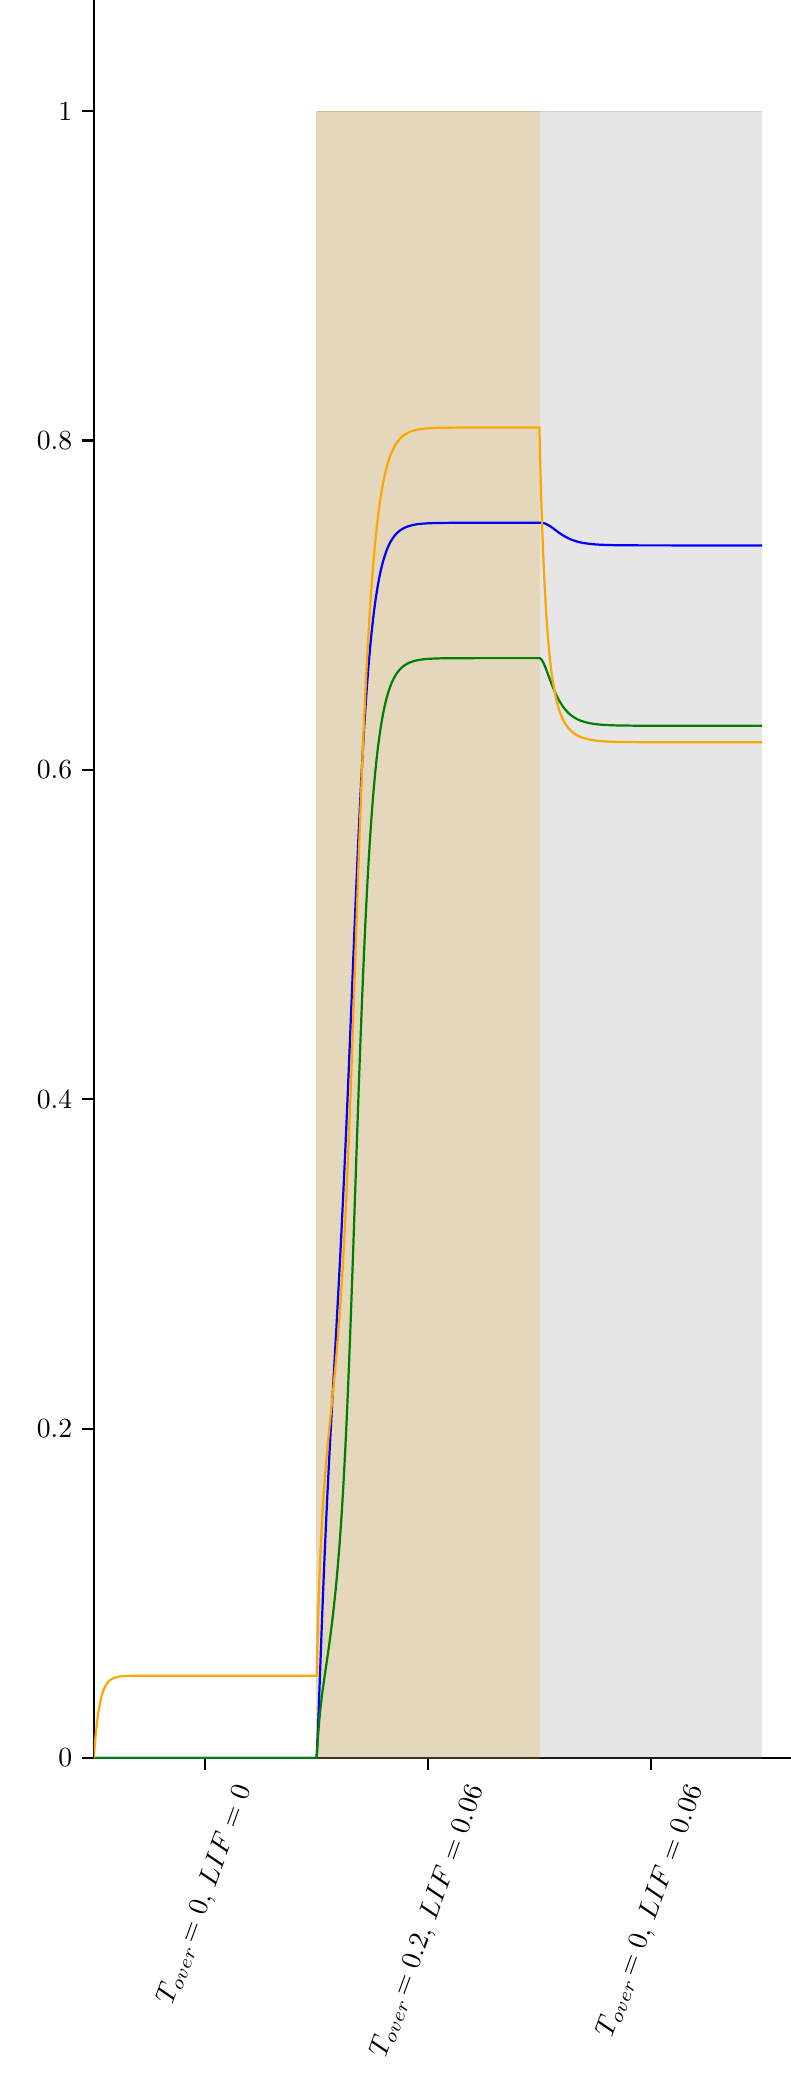
\begin{tikzpicture}[baseline]

\definecolor{darkgray176}{RGB}{176,176,176}
\definecolor{gray}{RGB}{128,128,128}
\definecolor{green}{RGB}{0,128,0}
\definecolor{lightgray204}{RGB}{204,204,204}
\definecolor{orange}{RGB}{255,165,0}

\begin{axis}[
 ytick={0,0.2,0.4,0.6,0.8,1},
 x tick label style = {rotate=70},
 y post scale=3, 
 transpose legend,
legend cell align={left},
legend style={
  fill opacity=0.8,
  draw opacity=1,
  text opacity=1,
  at={(axis cs:5,1.1)},
  anchor=south west,
    legend columns=4,
    /tikz/every even column/.append style={column sep=1.0cm},,
  draw=lightgray204
},
tick align=outside,
tick pos=left,
x grid style={darkgray176},
xmin=0, xmax=120,
xtick style={color=black},
xtick={20,60,100},
xticklabels={
  {\(\displaystyle T_\text{over}\!=0\), \(\displaystyle \text{LIF}=0\)},
  {\(\displaystyle T_\text{over}\!=0.2\), \(\displaystyle \text{LIF}=0.06\)},
  {\(\displaystyle T_\text{over}\!=0\), \(\displaystyle \text{LIF}=0.06\)}
},
y grid style={darkgray176},
ymin=0, ymax=1.05,
ytick style={color=black}
]
\path [draw=orange, fill=orange, opacity=0.2]
(axis cs:40,0)
--(axis cs:40,1)
--(axis cs:80,1)
--(axis cs:80,0)
--cycle;

\path [draw=gray, fill=gray, opacity=0.2]
(axis cs:40,0)
--(axis cs:40,1)
--(axis cs:120,1)
--(axis cs:120,0)
--cycle;

\addplot [thick, blue]
table {%
0 0
0.0001 0
0.0011 0
0.0111 0
0.1111 0
0.2111 0
0.3111 0
0.4111 0
0.5111 0
0.6111 0
0.7111 0
0.8111 0
0.9111 0
1.0111 0
1.1111 0
1.2111 0
1.3111 0
1.4111 0
1.5111 0
1.6111 0
1.7111 0
1.8111 0
1.9111 0
2.0111 0
2.1111 0
2.2111 0
2.3111 0
2.4111 0
2.5111 0
2.6111 0
2.7111 0
2.8111 0
2.9111 0
3.0111 0
3.1111 0
3.2111 0
3.3111 0
3.4111 0
3.5111 0
3.6111 0
3.7111 0
3.8111 0
3.9111 0
4.0111 0
4.1111 0
4.2111 0
4.3111 0
4.4111 0
4.5111 0
4.6111 0
4.7111 0
4.8111 0
4.9111 0
5.0111 0
5.1111 0
5.2111 0
5.3111 0
5.4111 0
5.5111 0
5.6111 0
5.7111 0
5.8111 0
5.9111 0
6.0111 0
6.1111 0
6.21109999999999 0
6.31109999999999 0
6.41109999999999 0
6.51109999999999 0
6.61109999999999 0
6.71109999999999 0
6.81109999999999 0
6.91109999999999 0
7.01109999999999 0
7.11109999999999 0
7.21109999999999 0
7.31109999999999 0
7.41109999999999 0
7.51109999999999 0
7.61109999999999 0
7.71109999999999 0
7.81109999999999 0
7.91109999999999 0
8.01109999999999 0
8.11109999999999 0
8.21109999999999 0
8.31109999999999 0
8.41109999999999 0
8.51109999999999 0
8.61109999999999 0
8.71109999999999 0
8.81109999999999 0
8.91109999999999 0
9.01109999999998 0
9.11109999999998 0
9.21109999999998 0
9.31109999999998 0
9.41109999999998 0
9.51109999999998 0
9.61109999999998 0
9.71109999999998 0
9.81109999999998 0
9.91109999999998 0
10.0111 0
10.1111 0
10.2111 0
10.3111 0
10.4111 0
10.5111 0
10.6111 0
10.7111 0
10.8111 0
10.9111 0
11.0111 0
11.1111 0
11.2111 0
11.3111 0
11.4111 0
11.5111 0
11.6111 0
11.7111 0
11.8111 0
11.9111 0
12.0111 0
12.1111 0
12.2111 0
12.3111 0
12.4111 0
12.5111 0
12.6111 0
12.7111 0
12.8111 0
12.9111 0
13.0111 0
13.1111 0
13.2111 0
13.3111 0
13.4111 0
13.5111 0
13.6111 0
13.7111 0
13.8111 0
13.9111 0
14.0111 0
14.1111 0
14.2111 0
14.3111 0
14.4111 0
14.5111 0
14.6111 0
14.7111 0
14.8111 0
14.9111 0
15.0111 0
15.1111 0
15.2111 0
15.3111 0
15.4111 0
15.5111 0
15.6111 0
15.7111 0
15.8111 0
15.9111 0
16.0111 0
16.1111 0
16.2111 0
16.3111 0
16.4111 0
16.5111 0
16.6111 0
16.7111 0
16.8111 0
16.9111 0
17.0111 0
17.1111 0
17.2111 0
17.3111 0
17.4111 0
17.5111 0
17.6111 0
17.7111 0
17.8111 0
17.9111 0
18.0111 0
18.1111 0
18.2111 0
18.3111 0
18.4111 0
18.5111 0
18.6111 0
18.7111 0
18.8111 0
18.9111 0
19.0111 0
19.1111 0
19.2111 0
19.3111 0
19.4111 0
19.5111 0
19.6111 0
19.7111 0
19.8111 0
19.9111 0
20.0111 0
20.1111 0
20.2111 0
20.3111 0
20.4111 0
20.5111 0
20.6111 0
20.7111 0
20.8111 0
20.9111 0
21.0111 0
21.1111 0
21.2111 0
21.3111 0
21.4111 0
21.5111 0
21.6111 0
21.7111 0
21.8111 0
21.9111 0
22.0111 0
22.1111 0
22.2111 0
22.3111 0
22.4111000000001 0
22.5111000000001 0
22.6111000000001 0
22.7111000000001 0
22.8111000000001 0
22.9111000000001 0
23.0111000000001 0
23.1111000000001 0
23.2111000000001 0
23.3111000000001 0
23.4111000000001 0
23.5111000000001 0
23.6111000000001 0
23.7111000000001 0
23.8111000000001 0
23.9111000000001 0
24.0111000000001 0
24.1111000000001 0
24.2111000000001 0
24.3111000000001 0
24.4111000000001 0
24.5111000000001 0
24.6111000000001 0
24.7111000000001 0
24.8111000000001 0
24.9111000000001 0
25.0111000000001 0
25.1111000000001 0
25.2111000000001 0
25.3111000000001 0
25.4111000000001 0
25.5111000000001 0
25.6111000000001 0
25.7111000000001 0
25.8111000000001 0
25.9111000000001 0
26.0111000000001 0
26.1111000000001 0
26.2111000000001 0
26.3111000000001 0
26.4111000000001 0
26.5111000000001 0
26.6111000000001 0
26.7111000000001 0
26.8111000000001 0
26.9111000000001 0
27.0111000000001 0
27.1111000000001 0
27.2111000000001 0
27.3111000000001 0
27.4111000000001 0
27.5111000000001 0
27.6111000000001 0
27.7111000000001 0
27.8111000000001 0
27.9111000000001 0
28.0111000000001 0
28.1111000000001 0
28.2111000000001 0
28.3111000000001 0
28.4111000000001 0
28.5111000000001 0
28.6111000000001 0
28.7111000000001 0
28.8111000000001 0
28.9111000000001 0
29.0111000000001 0
29.1111000000001 0
29.2111000000001 0
29.3111000000001 0
29.4111000000002 0
29.5111000000002 0
29.6111000000002 0
29.7111000000002 0
29.8111000000002 0
29.9111000000002 0
30.0111000000002 0
30.1111000000002 0
30.2111000000002 0
30.3111000000002 0
30.4111000000002 0
30.5111000000002 0
30.6111000000002 0
30.7111000000002 0
30.8111000000002 0
30.9111000000002 0
31.0111000000002 0
31.1111000000002 0
31.2111000000002 0
31.3111000000002 0
31.4111000000002 0
31.5111000000002 0
31.6111000000002 0
31.7111000000002 0
31.8111000000002 0
31.9111000000002 0
32.0111000000002 0
32.1111000000002 0
32.2111000000002 0
32.3111000000002 0
32.4111000000002 0
32.5111000000002 0
32.6111000000002 0
32.7111000000002 0
32.8111000000002 0
32.9111000000002 0
33.0111000000002 0
33.1111000000002 0
33.2111000000002 0
33.3111000000002 0
33.4111000000002 0
33.5111000000002 0
33.6111000000002 0
33.7111000000002 0
33.8111000000002 0
33.9111000000002 0
34.0111000000002 0
34.1111000000002 0
34.2111000000002 0
34.3111000000002 0
34.4111000000002 0
34.5111000000002 0
34.6111000000002 0
34.7111000000002 0
34.8111000000002 0
34.9111000000002 0
35.0111000000002 0
35.1111000000002 0
35.2111000000002 0
35.3111000000002 0
35.4111000000002 0
35.5111000000002 0
35.6111000000002 0
35.7111000000002 0
35.8111000000002 0
35.9111000000002 0
36.0111000000002 0
36.1111000000002 0
36.2111000000002 0
36.3111000000002 0
36.4111000000002 0
36.5111000000002 0
36.6111000000002 0
36.7111000000003 0
36.8111000000003 0
36.9111000000003 0
37.0111000000003 0
37.1111000000003 0
37.2111000000003 0
37.3111000000003 0
37.4111000000003 0
37.5111000000003 0
37.6111000000003 0
37.7111000000003 0
37.8111000000003 0
37.9111000000003 0
38.0111000000003 0
38.1111000000003 0
38.2111000000003 0
38.3111000000003 0
38.4111000000003 0
38.5111000000003 0
38.6111000000003 0
38.7111000000003 0
38.8111000000003 0
38.9111000000003 0
39.0111000000003 0
39.1111000000003 0
39.2111000000003 0
39.3111000000003 0
39.4111000000003 0
39.5111000000003 0
39.6111000000003 0
39.7111000000003 0
39.8111000000003 0
39.9111000000003 0
40 0
40 0
40.0115470977609 0.000702052242978834
40.1115470977609 0.0074722528644605
40.2115470977609 0.0152322853215913
40.311547097761 0.0236852379182537
40.411547097761 0.0325941095352077
40.511547097761 0.0417716096955924
40.611547097761 0.0510717672590983
40.711547097761 0.0603828411242505
40.811547097761 0.0696212460141488
40.911547097761 0.0787263329540813
41.011547097761 0.0876559265033558
41.111547097761 0.0963825455484119
41.211547097761 0.104890240658945
41.311547097761 0.113171980523111
41.411547097761 0.121227519018709
41.511547097761 0.129061675539409
41.611547097761 0.136682964699433
41.711547097761 0.144102516965956
41.811547097761 0.151333238323039
41.911547097761 0.158389164021062
42.011547097761 0.165284968262237
42.111547097761 0.172035597964818
42.211547097761 0.178656004350459
42.311547097761 0.185160950944565
42.411547097761 0.191564880680047
42.511547097761 0.197881828206789
42.611547097761 0.204125366310166
42.711547097761 0.21030857761653
42.811547097761 0.216444044593883
42.911547097761 0.22254385231704
43.011547097761 0.228619599624632
43.111547097761 0.234682415207103
43.211547097761 0.240742975878183
43.311547097761 0.246811524837407
43.411547097761 0.252897888161319
43.511547097761 0.259011488093963
43.611547097761 0.26516135196641
43.711547097761 0.271356115780428
43.811547097761 0.277604021659987
43.911547097761 0.283912908521348
44.011547097761 0.290290195451513
44.111547097761 0.296742857427997
44.211547097761 0.303277393171168
44.311547097761 0.309899785103465
44.411547097761 0.316615451605346
44.511547097761 0.323429192011482
44.611547097761 0.330345125084893
44.711547097761 0.337366622039863
44.811547097761 0.344496235550105
44.911547097761 0.351735626564581
45.011547097761 0.359085491140976
45.111547097761 0.366545489871522
45.211547097761 0.374114182787286
45.311547097761 0.381788972851431
45.411547097761 0.389566061254435
45.511547097761 0.397440417672891
45.611547097761 0.405405768423418
45.711547097761 0.413454605021134
45.811547097761 0.421578215040243
45.911547097761 0.429766736392591
46.011547097761 0.438009235226833
46.111547097761 0.446293806660663
46.211547097761 0.454607696557453
46.311547097761 0.4629374416179
46.411547097761 0.47126902424539
46.511547097761 0.479588038019116
46.611547097761 0.487879859213169
46.711547097761 0.496129819653854
46.811547097761 0.504323376310126
46.911547097761 0.512446273341647
47.011547097761 0.520484692847122
47.111547097761 0.528425391212715
47.211547097761 0.536255818701816
47.311547097761 0.543964220699258
47.4115470977611 0.551539719776853
47.5115470977611 0.558972378443032
47.6115470977611 0.566253243048568
47.7115470977611 0.573374369824534
47.8115470977611 0.580328834420048
47.9115470977611 0.587110726586464
48.0115470977611 0.593715131828955
48.1115470977611 0.600138101927558
48.2115470977611 0.60637661623241
48.3115470977611 0.612428535577515
48.4115470977611 0.618292550549265
48.5115470977611 0.62396812570431
48.6115470977611 0.629455441168675
48.7115470977611 0.634755332876708
48.8115470977611 0.639869232533082
48.9115470977611 0.644799108210019
49.0115470977611 0.649547406330046
49.1115470977611 0.654116995635009
49.2115470977611 0.658511113606791
49.3115470977611 0.662733315685057
49.4115470977611 0.666787427522625
49.5115470977611 0.67067750042918
49.6115470977611 0.674407770078269
49.7115470977611 0.677982618489765
49.8115470977611 0.681406539248891
49.9115470977611 0.684684105882352
50.0115470977611 0.687819943280677
50.1115470977611 0.690818702032373
50.2115470977611 0.693685035518718
50.3115470977611 0.696423579606946
50.4115470977611 0.699038934773209
50.5115470977611 0.701535650484167
50.6115470977611 0.703918211666656
50.7115470977611 0.706191027097907
50.8115470977611 0.708358419553714
50.9115470977611 0.710424617558298
51.0115470977611 0.71239374858695
51.1115470977611 0.714269833580632
51.2115470977611 0.716056782640126
51.3115470977611 0.717758391776046
51.4115470977611 0.719378340599703
51.5115470977611 0.720920190848384
51.6115470977611 0.722387385647012
51.7115470977611 0.723783249416184
51.8115470977611 0.725110988344341
51.9115470977611 0.726373691349101
52.0115470977611 0.727574331459752
52.1115470977611 0.728715767559308
52.2115470977611 0.729800746430627
52.3115470977611 0.730831905056674
52.4115470977611 0.731811773130194
52.5115470977611 0.732742775732864
52.6115470977611 0.733627236148359
52.7115470977611 0.734467378777813
52.8115470977611 0.735265332129803
52.9115470977611 0.736023131860342
53.0115470977611 0.736742723841381
53.1115470977611 0.737425967239094
53.2115470977611 0.738074637585661
53.3115470977611 0.738690429830541
53.4115470977611 0.73927496135919
53.5115470977611 0.739829774969029
53.6115470977611 0.740356341794021
53.7115470977611 0.7408560641707
53.8115470977611 0.741330278439744
53.9115470977611 0.741780257678327
54.0115470977611 0.742207214359477
54.1115470977611 0.742612302935576
54.2115470977611 0.742996622343872
54.3115470977611 0.743361218432603
54.4115470977612 0.743707086306886
54.5115470977612 0.74403517259405
54.6115470977612 0.744346377628565
54.7115470977612 0.744641557557045
54.8115470977612 0.744921526364189
54.9115470977612 0.745187057820758
55.0115470977612 0.745438887354943
55.1115470977612 0.74567771384865
55.2115470977612 0.745904201360415
55.3115470977612 0.746118980776759
55.4115470977612 0.746322651393911
55.5115470977612 0.746515782431897
55.6115470977612 0.746698914483054
55.7115470977612 0.746872560897056
55.8115470977612 0.747037209104566
55.9115470977612 0.747193321881631
56.0115470977612 0.74734133855695
56.1115470977612 0.747481676164096
56.2115470977612 0.74761473054079
56.3115470977612 0.74774087737726
56.4115470977612 0.747860473215709
56.5115470977612 0.747973856402862
56.6115470977612 0.748081347997506
56.7115470977612 0.748183252634914
56.8115470977612 0.748279859349978
56.9115470977612 0.74837144236081
57.0115470977612 0.748458261814544
57.1115470977612 0.748540564496999
57.2115470977612 0.7486185845078
57.3115470977612 0.748692543902527
57.4115470977612 0.748762653303364
57.5115470977612 0.748829112479706
57.6115470977612 0.748892110900101
57.7115470977612 0.748951828256861
57.8115470977612 0.749008434964613
57.9115470977612 0.749062092634028
58.0115470977612 0.74911295452189
58.1115470977612 0.749161165958644
58.2115470977612 0.749206864754494
58.3115470977612 0.74925018158508
58.4115470977612 0.749291240357733
58.5115470977612 0.749330158559235
58.6115470977612 0.749367047585999
58.7115470977612 0.749402013057523
58.8115470977612 0.749435155113939
58.9115470977612 0.74946656869844
59.0115470977612 0.749496343825339
59.1115470977612 0.749524565834465
59.2115470977612 0.74955131563258
59.3115470977612 0.749576669922459
59.4115470977612 0.749600701420255
59.5115470977612 0.749623479061738
59.6115470977612 0.749645068197955
59.7115470977612 0.749665530780854
59.8115470977612 0.749684925539381
59.9115470977612 0.749703308146517
60.0115470977612 0.749720731377722
60.1115470977612 0.749737245261231
60.2115470977612 0.749752897220593
60.3115470977612 0.749767732209873
60.4115470977612 0.749781792841867
60.5115470977612 0.749795119509707
60.6115470977612 0.749807750502177
60.7115470977612 0.749819722113071
60.8115470977612 0.749831068744898
60.9115470977612 0.749841823007213
61.0115470977612 0.749852015809869
61.1115470977612 0.749861676451427
61.2115470977612 0.749870832702996
61.3115470977612 0.749879510887716
61.4115470977613 0.749887735956129
61.5115470977613 0.749895531557636
61.6115470977613 0.749902920108242
61.7115470977613 0.74990992285479
61.8115470977613 0.749916559935857
61.9115470977613 0.749922850439488
62.0115470977613 0.749928812457925
62.1115470977613 0.749934463139498
62.2115470977613 0.749939818737815
62.3115470977613 0.749944894658397
62.4115470977613 0.749949705502881
62.5115470977613 0.74995426511093
62.6115470977613 0.74995858659996
62.7115470977613 0.749962682402799
62.8115470977613 0.749966564303385
62.9115470977613 0.749970243470607
63.0115470977613 0.749973730490383
63.1115470977613 0.749977035396066
63.2115470977613 0.749980167697272
63.3115470977613 0.749983136407197
63.4115470977613 0.749985950068516
63.5115470977613 0.749988616777935
63.6115470977613 0.749991144209458
63.7115470977613 0.749993539636443
63.8115470977613 0.749995809952513
63.9115470977613 0.749997961691365
64.0115470977613 0.750000001045561
64.1115470977613 0.750001933884329
64.2115470977613 0.750003765770439
64.3115470977613 0.750005501976199
64.4115470977613 0.750007147498613
64.5115470977613 0.750008707073758
64.6115470977612 0.750010185190399
64.7115470977612 0.750011586102901
64.8115470977612 0.750012913843467
64.9115470977612 0.750014172233734
65.0115470977612 0.750015364895769
65.1115470977612 0.750016495262483
65.2115470977612 0.750017566587515
65.3115470977612 0.750018581954583
65.4115470977612 0.750019544286363
65.5115470977612 0.750020456352895
65.6115470977612 0.750021320779551
65.7115470977612 0.750022140054593
65.8115470977612 0.750022916536328
65.9115470977612 0.750023652459899
66.0115470977612 0.750024349943712
66.1115470977612 0.750025010995535
66.2115470977612 0.750025637518272
66.3115470977611 0.750026231315444
66.4115470977611 0.750026794096376
66.5115470977611 0.750027327481114
66.6115470977611 0.750027833005093
66.7115470977611 0.750028312123552
66.8115470977611 0.750028766215721
66.9115470977611 0.750029196588796
67.0115470977611 0.750029604481693
67.1115470977611 0.750029991068623
67.2115470977611 0.750030357462464
67.3115470977611 0.750030704717968
67.4115470977611 0.750031033834795
67.5115470977611 0.750031345760392
67.6115470977611 0.750031641392718
67.7115470977611 0.750031921582832
67.8115470977611 0.750032187137339
67.9115470977611 0.750032438820711
68.0115470977611 0.750032677357494
68.111547097761 0.750032903434387
68.211547097761 0.750033117702219
68.311547097761 0.750033320777827
68.411547097761 0.750033513245828
68.511547097761 0.750033695660302
68.611547097761 0.750033868546388
68.711547097761 0.750034032401795
68.811547097761 0.750034187698236
68.911547097761 0.750034334882784
69.011547097761 0.750034474379158
69.111547097761 0.750034606588948
69.211547097761 0.750034731892764
69.311547097761 0.750034850651339
69.411547097761 0.75003496320656
69.511547097761 0.750035069882457
69.611547097761 0.750035170986136
69.711547097761 0.75003526680866
69.811547097761 0.750035357625889
69.9115470977609 0.750035443699273
70.0115470977609 0.750035525276606
70.1115470977609 0.75003560259274
70.2115470977609 0.750035675870257
70.3115470977609 0.750035745320114
70.4115470977609 0.750035811142248
70.5115470977609 0.750035873526155
70.6115470977609 0.750035932651428
70.7115470977609 0.750035988688283
70.8115470977609 0.750036041798044
70.9115470977609 0.750036092133607
71.0115470977609 0.750036139839883
71.1115470977609 0.750036185054213
71.2115470977609 0.750036227906762
71.3115470977609 0.750036268520901
71.4115470977609 0.750036307013551
71.5115470977609 0.750036343495529
71.6115470977608 0.750036378071863
71.7115470977608 0.750036410842095
71.8115470977608 0.750036441900566
71.9115470977608 0.75003647133669
72.0115470977608 0.750036499235211
72.1115470977608 0.750036525676446
72.2115470977608 0.750036550736516
72.3115470977608 0.750036574487568
72.4115470977608 0.750036596997977
72.5115470977608 0.750036618332549
72.6115470977608 0.750036638552704
72.7115470977608 0.750036657716654
72.8115470977608 0.750036675879569
72.9115470977608 0.75003669309374
73.0115470977608 0.750036709408724
73.1115470977608 0.75003672487149
73.2115470977608 0.750036739526554
73.3115470977608 0.750036753416107
73.4115470977607 0.750036766580135
73.5115470977607 0.750036779056537
73.6115470977607 0.750036790881229
73.7115470977607 0.750036802088256
73.8115470977607 0.75003681270988
73.9115470977607 0.750036822776681
74.0115470977607 0.750036832317639
74.1115470977607 0.750036841360223
74.2115470977607 0.750036849930464
74.3115470977607 0.750036858053036
74.4115470977607 0.750036865751323
74.5115470977607 0.750036873047488
74.6115470977607 0.750036879962536
74.7115470977607 0.750036886516374
74.8115470977607 0.75003689272787
74.9115470977607 0.750036898614907
75.0115470977607 0.750036904194432
75.1115470977606 0.75003690948251
75.2115470977606 0.750036914494363
75.3115470977606 0.75003691924442
75.4115470977606 0.750036923746357
75.5115470977606 0.750036928013133
75.6115470977606 0.750036932057033
75.7115470977606 0.750036935889699
75.8115470977606 0.750036939522164
75.9115470977606 0.750036942964886
76.0115470977606 0.750036946227777
76.1115470977606 0.750036949320229
76.2115470977606 0.750036952251147
76.3115470977606 0.750036955028967
76.4115470977606 0.750036957661686
76.5115470977606 0.750036960156885
76.6115470977606 0.750036962521746
76.7115470977606 0.750036964763078
76.8115470977606 0.750036966887333
76.9115470977605 0.750036968900627
77.0115470977605 0.750036970808756
77.1115470977605 0.750036972617213
77.2115470977605 0.750036974331205
77.3115470977605 0.750036975955666
77.4115470977605 0.750036977495273
77.5115470977605 0.750036978954458
77.6115470977605 0.750036980337421
77.7115470977605 0.750036981648146
77.8115470977605 0.750036982890404
77.9115470977605 0.750036984067772
78.0115470977605 0.750036985183641
78.1115470977605 0.750036986241221
78.2115470977605 0.750036987243558
78.3115470977605 0.750036988193538
78.4115470977605 0.750036989093896
78.5115470977605 0.750036989947223
78.6115470977605 0.750036990755976
78.7115470977604 0.750036991522484
78.8115470977604 0.750036992248953
78.9115470977604 0.750036992937475
79.0115470977604 0.750036993590031
79.1115470977604 0.750036994208501
79.2115470977604 0.750036994794665
79.3115470977604 0.750036995350211
79.4115470977604 0.750036995876737
79.5115470977604 0.75003699637576
79.6115470977604 0.750036996848717
79.7115470977604 0.750036997296968
79.8115470977604 0.750036997721805
79.9115470977604 0.750036998124451
80 0.750036998463037
80 0.750036998463037
80.1 0.750036266486613
80.2 0.75003143070575
80.3 0.750019136697197
80.4 0.749996754046436
80.5 0.749962282541768
80.6 0.749914267506455
80.7 0.749851723549997
80.8 0.749774066084854
80.8999999999999 0.749681050005672
80.9999999999999 0.749572714968982
81.0999999999999 0.749449336745518
81.1999999999999 0.749311384147315
81.2999999999999 0.749159481059132
81.3999999999999 0.748994373129614
81.4999999999999 0.748816898702731
81.5999999999999 0.748627963594591
81.6999999999999 0.748428519345114
81.7999999999999 0.748219544598067
81.8999999999999 0.748002029286737
81.9999999999999 0.747776961325766
82.0999999999999 0.747545315532434
82.1999999999999 0.747308044522692
82.2999999999999 0.747066071348454
82.3999999999999 0.746820283662964
82.4999999999999 0.746571529220334
82.5999999999999 0.74632061253361
82.6999999999998 0.746068292532834
82.7999999999998 0.745815281080621
82.8999999999998 0.745562242217634
82.9999999999998 0.745309792024175
83.0999999999998 0.745058498996783
83.1999999999998 0.74480888485041
83.2999999999998 0.744561425667389
83.3999999999998 0.744316553324121
83.4999999999998 0.744074657135152
83.5999999999998 0.743836085662318
83.6999999999998 0.743601148643693
83.7999999999998 0.743370119003557
83.8999999999998 0.743143234910245
83.9999999999998 0.742920701853893
84.0999999999998 0.742702694720542
84.1999999999998 0.742489359843111
84.2999999999998 0.742280817013192
84.3999999999997 0.742077161440734
84.4999999999997 0.741878465651345
84.5999999999997 0.741684781313261
84.6999999999997 0.74149614098805
84.7999999999997 0.741312559800839
84.8999999999997 0.741134037027325
84.9999999999997 0.740960557596083
85.0999999999997 0.740792093505744
85.1999999999997 0.740628605157468
85.2999999999997 0.740470042603896
85.3999999999997 0.74031634671633
85.4999999999997 0.740167450272371
85.5999999999997 0.740023278966613
85.6999999999997 0.73988375234729
85.7999999999997 0.73974878468195
85.8999999999997 0.739618285755416
85.9999999999997 0.739492161603339
86.0999999999997 0.739370315184728
86.1999999999996 0.739252646996823
86.2999999999996 0.739139055635657
86.3999999999996 0.739029438305597
86.4999999999996 0.738923691281086
86.5999999999996 0.738821710323701
86.6999999999996 0.738723391057548
86.7999999999996 0.738628629305895
86.8999999999996 0.738537321391824
86.9999999999996 0.738449364405554
87.0999999999996 0.73836465644095
87.1999999999996 0.738283096803618
87.2999999999996 0.73820458619284
87.3999999999996 0.738129026859479
87.4999999999996 0.738056322741861
87.5999999999996 0.737986379581506
87.6999999999996 0.737919105020473
87.7999999999996 0.737854408681969
87.8999999999996 0.737792202235732
87.9999999999995 0.73773239944964
88.0999999999995 0.737674916228856
88.1999999999995 0.737619670643729
88.2999999999995 0.737566582947615
88.3999999999995 0.73751557558563
88.4999999999995 0.737466573195336
88.5999999999995 0.737419502600232
88.6999999999995 0.73737429279688
88.7999999999995 0.737330874936407
88.8999999999995 0.737289182301086
88.9999999999995 0.737249150276611
89.0999999999995 0.737210716320658
89.1999999999995 0.737173819928235
89.2999999999995 0.737138402594322
89.3999999999995 0.737104407774213
89.4999999999995 0.737071780841967
89.5999999999995 0.737040469047314
89.6999999999994 0.737010421471336
89.7999999999994 0.73698158898122
89.8999999999994 0.736953924184331
89.9999999999994 0.736927381381842
90.0999999999994 0.736901916522127
90.1999999999994 0.736877487154094
90.2999999999994 0.736854052380638
90.3999999999994 0.736831572812338
90.4999999999994 0.736810010521534
90.5999999999994 0.736789328996898
90.6999999999994 0.736769493098586
90.7999999999994 0.736750469014061
90.8999999999994 0.736732224214657
90.9999999999994 0.736714727412937
91.0999999999994 0.736697948520911
91.1999999999994 0.736681858609134
91.2999999999994 0.736666429866741
91.3999999999994 0.736651635562429
91.4999999999993 0.736637450006409
91.5999999999993 0.736623848513349
91.6999999999993 0.736610807366314
91.7999999999993 0.736598303781705
91.8999999999993 0.736586315875197
91.9999999999993 0.736574822628686
92.0999999999993 0.736563803858219
92.1999999999993 0.736553240182913
92.2999999999993 0.736543112994852
92.3999999999993 0.736533404429939
92.4999999999993 0.736524097339696
92.5999999999993 0.736515175263996
92.6999999999993 0.736506622404705
92.7999999999993 0.736498423600219
92.8999999999993 0.736490564300873
92.9999999999993 0.736483030545209
93.0999999999993 0.736475808937069
93.1999999999992 0.736468886623511
93.2999999999992 0.736462251273505
93.3999999999992 0.736455891057405
93.4999999999992 0.736449794627166
93.5999999999992 0.736443951097287
93.6999999999992 0.73643835002646
93.7999999999992 0.736432981399896
93.8999999999992 0.736427835612322
93.9999999999992 0.736422903451609
94.0999999999992 0.736418176083025
94.1999999999992 0.736413645034088
94.2999999999992 0.736409302179997
94.3999999999992 0.736405139729621
94.4999999999992 0.736401150212036
94.5999999999992 0.736397326463574
94.6999999999992 0.736393661615383
94.7999999999992 0.736390149081474
94.8999999999992 0.736386782547231
94.9999999999991 0.736383555958376
95.0999999999991 0.736380463510369
95.1999999999991 0.736377499638229
95.2999999999991 0.736374659006755
95.3999999999991 0.736371936501143
95.4999999999991 0.736369327217966
95.5999999999991 0.736366826456525
95.6999999999991 0.736364429710543
95.7999999999991 0.736362132660191
95.8999999999991 0.736359931164435
95.9999999999991 0.736357821253693
96.0999999999991 0.736355799122788
96.1999999999991 0.736353861124184
96.2999999999991 0.7363520037615
96.3999999999991 0.736350223683281
96.4999999999991 0.736348517677029
96.5999999999991 0.736346882663471
96.6999999999991 0.736345315691064
96.799999999999 0.736343813930721
96.899999999999 0.736342374670758
96.999999999999 0.736340995312039
97.099999999999 0.736339673363325
97.199999999999 0.736338406436817
97.299999999999 0.736337192243871
97.399999999999 0.736336028590898
97.499999999999 0.736334913375431
97.599999999999 0.736333844582348
97.699999999999 0.736332820280256
97.799999999999 0.736331838618025
97.899999999999 0.736330897821454
97.999999999999 0.73632999619009
98.099999999999 0.736329132094164
98.199999999999 0.736328303971665
98.299999999999 0.736327510325522
98.399999999999 0.736326749720917
98.4999999999989 0.736326020782696
98.5999999999989 0.736325322192895
98.6999999999989 0.736324652688365
98.7999999999989 0.736324011058495
98.8999999999989 0.736323396143033
98.9999999999989 0.73632280682999
99.0999999999989 0.736322242053638
99.1999999999989 0.73632170079259
99.2999999999989 0.73632118206795
99.3999999999989 0.736320684941557
99.4999999999989 0.736320208514283
99.5999999999989 0.736319751924417
99.6999999999989 0.736319314346106
99.7999999999989 0.736318894987864
99.8999999999989 0.736318493091147
99.9999999999989 0.736318107928979
100.099999999999 0.736317738804639
100.199999999999 0.736317385050407
100.299999999999 0.736317046026353
100.399999999999 0.736316721119185
100.499999999999 0.736316409741138
100.599999999999 0.736316111328913
100.699999999999 0.73631582534266
100.799999999999 0.736315551265
100.899999999999 0.736315288600095
100.999999999999 0.736315036872746
101.099999999999 0.736314795627536
101.199999999999 0.73631456442801
101.299999999999 0.736314342855881
101.399999999999 0.736314130510278
101.499999999999 0.736313927007017
101.599999999999 0.736313731977912
101.699999999999 0.736313545070103
101.799999999999 0.736313365945425
101.899999999999 0.736313194279788
101.999999999999 0.736313029762598
102.099999999999 0.736312872096195
102.199999999999 0.736312720995307
102.299999999999 0.736312576186546
102.399999999999 0.736312437407902
102.499999999999 0.736312304408278
102.599999999999 0.73631217694703
102.699999999999 0.736312054793534
102.799999999999 0.736311937726771
102.899999999999 0.736311825534922
102.999999999999 0.736311718014989
103.099999999999 0.736311614972429
103.199999999999 0.736311516220795
103.299999999999 0.736311421581408
103.399999999999 0.736311330883027
103.499999999999 0.736311243961541
103.599999999999 0.736311160659674
103.699999999999 0.736311080826698
103.799999999999 0.736311004318163
103.899999999999 0.736310930995631
103.999999999999 0.736310860726431
104.099999999999 0.736310793383417
104.199999999999 0.736310728844735
104.299999999999 0.736310666993608
104.399999999999 0.736310607718119
104.499999999999 0.736310550911013
104.599999999999 0.736310496469502
104.699999999999 0.736310444295076
104.799999999999 0.736310394293329
104.899999999999 0.736310346373785
104.999999999999 0.736310300449736
105.099999999999 0.736310256438086
105.199999999999 0.736310214259197
105.299999999999 0.736310173836748
105.399999999999 0.736310135097597
105.499999999999 0.736310097971647
105.599999999999 0.736310062391721
105.699999999999 0.736310028293438
105.799999999999 0.736309995615099
105.899999999999 0.736309964297573
105.999999999999 0.736309934284194
106.099999999999 0.736309905520652
106.199999999999 0.736309877954901
106.299999999999 0.736309851537063
106.399999999998 0.736309826219335
106.499999999998 0.736309801955905
106.599999999998 0.736309778702871
106.699999999998 0.736309756418155
106.799999999998 0.736309735061436
106.899999999998 0.736309714594069
106.999999999998 0.736309694979018
107.099999999998 0.736309676180791
107.199999999998 0.736309658165374
107.299999999998 0.736309640900167
107.399999999998 0.736309624353931
107.499999999998 0.736309608496725
107.599999999998 0.736309593299856
107.699999999998 0.736309578735826
107.799999999998 0.736309564778283
107.899999999998 0.736309551401969
107.999999999998 0.736309538582682
108.099999999998 0.736309526297224
108.199999999998 0.736309514523367
108.299999999998 0.736309503239805
108.399999999998 0.736309492426122
108.499999999998 0.736309482062749
108.599999999998 0.736309472130936
108.699999999998 0.736309462612711
108.799999999998 0.736309453490851
108.899999999998 0.736309444748849
108.999999999998 0.736309436370889
109.099999999998 0.73630942834181
109.199999999998 0.736309420647083
109.299999999998 0.736309413272786
109.399999999998 0.736309406205575
109.499999999998 0.736309399432661
109.599999999998 0.736309392941791
109.699999999998 0.736309386721218
109.799999999998 0.736309380759686
109.899999999998 0.736309375046409
109.999999999998 0.736309369571049
110.099999999998 0.736309364323697
110.199999999998 0.73630935929486
110.299999999998 0.736309354475437
110.399999999998 0.736309349856708
110.499999999998 0.736309345430315
110.599999999998 0.73630934118825
110.699999999998 0.736309337122835
110.799999999998 0.736309333226716
110.899999999998 0.736309329492842
110.999999999998 0.736309325914456
111.099999999998 0.736309322485084
111.199999999998 0.73630931919852
111.299999999998 0.736309316048818
111.399999999998 0.736309313030279
111.499999999998 0.736309310137439
111.599999999998 0.736309307365065
111.699999999998 0.73630930470814
111.799999999998 0.736309302161857
111.899999999998 0.736309299721608
111.999999999998 0.736309297382978
112.099999999998 0.736309295141735
112.199999999998 0.736309292993823
112.299999999998 0.736309290935356
112.399999999998 0.736309288962609
112.499999999998 0.736309287072013
112.599999999998 0.736309285260146
112.699999999998 0.736309283523731
112.799999999998 0.736309281859624
112.899999999998 0.736309280264816
112.999999999998 0.736309278736419
113.099999999998 0.736309277271669
113.199999999998 0.736309275867916
113.299999999998 0.736309274522618
113.399999999998 0.736309273233342
113.499999999998 0.736309271997756
113.599999999998 0.736309270813622
113.699999999998 0.736309269678799
113.799999999998 0.736309268591233
113.899999999998 0.736309267548957
113.999999999998 0.736309266550083
114.099999999998 0.736309265592806
114.199999999998 0.736309264675392
114.299999999998 0.736309263796181
114.399999999998 0.736309262953584
114.499999999998 0.736309262146074
114.599999999998 0.736309261372191
114.699999999998 0.736309260630535
114.799999999998 0.736309259919764
114.899999999998 0.736309259238591
114.999999999998 0.736309258585784
115.099999999998 0.736309257960161
115.199999999998 0.736309257360591
115.299999999998 0.736309256785989
115.399999999998 0.736309256235315
115.499999999998 0.736309255707572
115.599999999998 0.736309255201806
115.699999999998 0.736309254717102
115.799999999998 0.736309254252582
115.899999999998 0.736309253807405
115.999999999998 0.736309253380768
116.099999999998 0.736309252971896
116.199999999998 0.736309252580051
116.299999999998 0.736309252204524
116.399999999998 0.736309251844634
116.499999999998 0.736309251499732
116.599999999998 0.736309251169192
116.699999999998 0.736309250852416
116.799999999998 0.736309250548832
116.899999999998 0.73630925025789
116.999999999998 0.736309249979064
117.099999999998 0.736309249711849
117.199999999998 0.736309249455761
117.299999999998 0.736309249210337
117.399999999998 0.736309248975134
117.499999999998 0.736309248749725
117.599999999998 0.736309248533703
117.699999999998 0.736309248326676
117.799999999998 0.736309248128271
117.899999999998 0.736309247938128
117.999999999998 0.736309247755902
118.099999999998 0.736309247581266
118.199999999998 0.736309247413901
118.299999999998 0.736309247253506
118.399999999998 0.736309247099791
118.499999999998 0.736309246952476
118.599999999998 0.736309246811296
118.699999999998 0.736309246675996
118.799999999998 0.736309246546329
118.899999999998 0.736309246422062
118.999999999998 0.73630924630297
119.099999999998 0.736309246188837
119.199999999998 0.736309246079457
119.299999999998 0.736309245974632
119.399999999998 0.736309245874173
119.499999999998 0.736309245777896
119.599999999998 0.736309245685629
119.699999999998 0.736309245597204
119.799999999998 0.736309245512461
119.899999999998 0.736309245431247
119.999999999998 0.736309245353416
120 0.736309245353416
};
\addplot [thick, green]
table {%
0 0
0.0001 0
0.0011 0
0.0111 0
0.1111 0
0.2111 0
0.3111 0
0.4111 0
0.5111 0
0.6111 0
0.7111 0
0.8111 0
0.9111 0
1.0111 0
1.1111 0
1.2111 0
1.3111 0
1.4111 0
1.5111 0
1.6111 0
1.7111 0
1.8111 0
1.9111 0
2.0111 0
2.1111 0
2.2111 0
2.3111 0
2.4111 0
2.5111 0
2.6111 0
2.7111 0
2.8111 0
2.9111 0
3.0111 0
3.1111 0
3.2111 0
3.3111 0
3.4111 0
3.5111 0
3.6111 0
3.7111 0
3.8111 0
3.9111 0
4.0111 0
4.1111 0
4.2111 0
4.3111 0
4.4111 0
4.5111 0
4.6111 0
4.7111 0
4.8111 0
4.9111 0
5.0111 0
5.1111 0
5.2111 0
5.3111 0
5.4111 0
5.5111 0
5.6111 0
5.7111 0
5.8111 0
5.9111 0
6.0111 0
6.1111 0
6.21109999999999 0
6.31109999999999 0
6.41109999999999 0
6.51109999999999 0
6.61109999999999 0
6.71109999999999 0
6.81109999999999 0
6.91109999999999 0
7.01109999999999 0
7.11109999999999 0
7.21109999999999 0
7.31109999999999 0
7.41109999999999 0
7.51109999999999 0
7.61109999999999 0
7.71109999999999 0
7.81109999999999 0
7.91109999999999 0
8.01109999999999 0
8.11109999999999 0
8.21109999999999 0
8.31109999999999 0
8.41109999999999 0
8.51109999999999 0
8.61109999999999 0
8.71109999999999 0
8.81109999999999 0
8.91109999999999 0
9.01109999999998 0
9.11109999999998 0
9.21109999999998 0
9.31109999999998 0
9.41109999999998 0
9.51109999999998 0
9.61109999999998 0
9.71109999999998 0
9.81109999999998 0
9.91109999999998 0
10.0111 0
10.1111 0
10.2111 0
10.3111 0
10.4111 0
10.5111 0
10.6111 0
10.7111 0
10.8111 0
10.9111 0
11.0111 0
11.1111 0
11.2111 0
11.3111 0
11.4111 0
11.5111 0
11.6111 0
11.7111 0
11.8111 0
11.9111 0
12.0111 0
12.1111 0
12.2111 0
12.3111 0
12.4111 0
12.5111 0
12.6111 0
12.7111 0
12.8111 0
12.9111 0
13.0111 0
13.1111 0
13.2111 0
13.3111 0
13.4111 0
13.5111 0
13.6111 0
13.7111 0
13.8111 0
13.9111 0
14.0111 0
14.1111 0
14.2111 0
14.3111 0
14.4111 0
14.5111 0
14.6111 0
14.7111 0
14.8111 0
14.9111 0
15.0111 0
15.1111 0
15.2111 0
15.3111 0
15.4111 0
15.5111 0
15.6111 0
15.7111 0
15.8111 0
15.9111 0
16.0111 0
16.1111 0
16.2111 0
16.3111 0
16.4111 0
16.5111 0
16.6111 0
16.7111 0
16.8111 0
16.9111 0
17.0111 0
17.1111 0
17.2111 0
17.3111 0
17.4111 0
17.5111 0
17.6111 0
17.7111 0
17.8111 0
17.9111 0
18.0111 0
18.1111 0
18.2111 0
18.3111 0
18.4111 0
18.5111 0
18.6111 0
18.7111 0
18.8111 0
18.9111 0
19.0111 0
19.1111 0
19.2111 0
19.3111 0
19.4111 0
19.5111 0
19.6111 0
19.7111 0
19.8111 0
19.9111 0
20.0111 0
20.1111 0
20.2111 0
20.3111 0
20.4111 0
20.5111 0
20.6111 0
20.7111 0
20.8111 0
20.9111 0
21.0111 0
21.1111 0
21.2111 0
21.3111 0
21.4111 0
21.5111 0
21.6111 0
21.7111 0
21.8111 0
21.9111 0
22.0111 0
22.1111 0
22.2111 0
22.3111 0
22.4111000000001 0
22.5111000000001 0
22.6111000000001 0
22.7111000000001 0
22.8111000000001 0
22.9111000000001 0
23.0111000000001 0
23.1111000000001 0
23.2111000000001 0
23.3111000000001 0
23.4111000000001 0
23.5111000000001 0
23.6111000000001 0
23.7111000000001 0
23.8111000000001 0
23.9111000000001 0
24.0111000000001 0
24.1111000000001 0
24.2111000000001 0
24.3111000000001 0
24.4111000000001 0
24.5111000000001 0
24.6111000000001 0
24.7111000000001 0
24.8111000000001 0
24.9111000000001 0
25.0111000000001 0
25.1111000000001 0
25.2111000000001 0
25.3111000000001 0
25.4111000000001 0
25.5111000000001 0
25.6111000000001 0
25.7111000000001 0
25.8111000000001 0
25.9111000000001 0
26.0111000000001 0
26.1111000000001 0
26.2111000000001 0
26.3111000000001 0
26.4111000000001 0
26.5111000000001 0
26.6111000000001 0
26.7111000000001 0
26.8111000000001 0
26.9111000000001 0
27.0111000000001 0
27.1111000000001 0
27.2111000000001 0
27.3111000000001 0
27.4111000000001 0
27.5111000000001 0
27.6111000000001 0
27.7111000000001 0
27.8111000000001 0
27.9111000000001 0
28.0111000000001 0
28.1111000000001 0
28.2111000000001 0
28.3111000000001 0
28.4111000000001 0
28.5111000000001 0
28.6111000000001 0
28.7111000000001 0
28.8111000000001 0
28.9111000000001 0
29.0111000000001 0
29.1111000000001 0
29.2111000000001 0
29.3111000000001 0
29.4111000000002 0
29.5111000000002 0
29.6111000000002 0
29.7111000000002 0
29.8111000000002 0
29.9111000000002 0
30.0111000000002 0
30.1111000000002 0
30.2111000000002 0
30.3111000000002 0
30.4111000000002 0
30.5111000000002 0
30.6111000000002 0
30.7111000000002 0
30.8111000000002 0
30.9111000000002 0
31.0111000000002 0
31.1111000000002 0
31.2111000000002 0
31.3111000000002 0
31.4111000000002 0
31.5111000000002 0
31.6111000000002 0
31.7111000000002 0
31.8111000000002 0
31.9111000000002 0
32.0111000000002 0
32.1111000000002 0
32.2111000000002 0
32.3111000000002 0
32.4111000000002 0
32.5111000000002 0
32.6111000000002 0
32.7111000000002 0
32.8111000000002 0
32.9111000000002 0
33.0111000000002 0
33.1111000000002 0
33.2111000000002 0
33.3111000000002 0
33.4111000000002 0
33.5111000000002 0
33.6111000000002 0
33.7111000000002 0
33.8111000000002 0
33.9111000000002 0
34.0111000000002 0
34.1111000000002 0
34.2111000000002 0
34.3111000000002 0
34.4111000000002 0
34.5111000000002 0
34.6111000000002 0
34.7111000000002 0
34.8111000000002 0
34.9111000000002 0
35.0111000000002 0
35.1111000000002 0
35.2111000000002 0
35.3111000000002 0
35.4111000000002 0
35.5111000000002 0
35.6111000000002 0
35.7111000000002 0
35.8111000000002 0
35.9111000000002 0
36.0111000000002 0
36.1111000000002 0
36.2111000000002 0
36.3111000000002 0
36.4111000000002 0
36.5111000000002 0
36.6111000000002 0
36.7111000000003 0
36.8111000000003 0
36.9111000000003 0
37.0111000000003 0
37.1111000000003 0
37.2111000000003 0
37.3111000000003 0
37.4111000000003 0
37.5111000000003 0
37.6111000000003 0
37.7111000000003 0
37.8111000000003 0
37.9111000000003 0
38.0111000000003 0
38.1111000000003 0
38.2111000000003 0
38.3111000000003 0
38.4111000000003 0
38.5111000000003 0
38.6111000000003 0
38.7111000000003 0
38.8111000000003 0
38.9111000000003 0
39.0111000000003 0
39.1111000000003 0
39.2111000000003 0
39.3111000000003 0
39.4111000000003 0
39.5111000000003 0
39.6111000000003 0
39.7111000000003 0
39.8111000000003 0
39.9111000000003 0
40 0
40 0
40.0115470977609 0.000688841162975454
40.1115470977609 0.00633315363817353
40.2115470977609 0.0114418659799412
40.311547097761 0.0160705705048354
40.411547097761 0.0202736866676503
40.511547097761 0.0241044511262795
40.611547097761 0.0276142161558378
40.711547097761 0.030851513649397
40.811547097761 0.033861213436914
40.911547097761 0.0366839483545856
41.011547097761 0.039355852818379
41.111547097761 0.0419085831986774
41.211547097761 0.044369552019362
41.311547097761 0.0467623009298712
41.411547097761 0.0491069464849677
41.511547097761 0.0514206482690337
41.611547097761 0.053718064889302
41.711547097761 0.0560117769480597
41.811547097761 0.058312666367363
41.911547097761 0.0606302485183981
42.011547097761 0.0629729580819096
42.111547097761 0.0653483921103822
42.211547097761 0.067763514979195
42.311547097761 0.0702248302762001
42.411547097761 0.0727385245299485
42.511547097761 0.0753105872493458
42.611547097761 0.0779469111918793
42.711547097761 0.0806533761847294
42.811547097761 0.0834359192442188
42.911547097761 0.0863005931997284
43.011547097761 0.0892536155382162
43.111547097761 0.0923014087455578
43.211547097761 0.0954506330270577
43.311547097761 0.0987082119356656
43.411547097761 0.102081351116433
43.511547097761 0.105577550084215
43.611547097761 0.109204606684823
43.711547097761 0.112970613646204
43.811547097761 0.116883946406739
43.911547097761 0.120953241216419
44.011547097761 0.125187362350519
44.111547097761 0.129595357165065
44.211547097761 0.134186397672705
44.311547097761 0.138969707343463
44.411547097761 0.143954471956516
44.511547097761 0.14914973356679
44.611547097761 0.154564267023088
44.711547097761 0.160206438998231
44.811547097761 0.166084050174825
44.911547097761 0.172204162070256
45.011547097761 0.178572910963834
45.111547097761 0.185195312471621
45.211547097761 0.192075061443445
45.311547097761 0.199214332954276
45.411547097761 0.206613591133182
45.511547097761 0.214271413311048
45.611547097761 0.222184337366329
45.711547097761 0.230346740111838
45.811547097761 0.238750754028255
45.911547097761 0.247386228585223
46.011547097761 0.256240740823384
46.111547097761 0.265299657879204
46.211547097761 0.274546251848295
46.311547097761 0.283961864969666
46.411547097761 0.293526120760344
46.511547097761 0.3032171746221
46.611547097761 0.313011995740295
46.711547097761 0.322886670916795
46.811547097761 0.332816720388027
46.911547097761 0.342777415680912
47.011547097761 0.352744090105702
47.111547097761 0.362692433485324
47.211547097761 0.372598764057656
47.311547097761 0.382440272030752
47.4115470977611 0.392195230894788
47.5115470977611 0.401843174186634
47.6115470977611 0.41136503687371
47.7115470977611 0.420743261809119
47.8115470977611 0.429961872771765
47.9115470977611 0.439006516428001
48.0115470977611 0.447864476139107
48.1115470977611 0.456524660909321
48.2115470977611 0.464977572949139
48.3115470977611 0.473215257350028
48.4115470977611 0.481231237262651
48.5115470977611 0.489020437773122
48.6115470977611 0.4965791014097
48.7115470977611 0.5039046979106
48.8115470977611 0.510995830562912
48.9115470977611 0.517852141099251
49.0115470977611 0.524474214824918
49.1115470977611 0.530863487352749
49.2115470977611 0.537022154051168
49.3115470977611 0.542953083066444
49.4115470977611 0.548659732564218
49.5115470977611 0.554146072647877
49.6115470977611 0.55941651225129
49.7115470977611 0.564475831168958
49.8115470977611 0.569329117275622
49.9115470977611 0.573981708897412
50.0115470977611 0.578439142225229
50.1115470977611 0.582707103605842
50.2115470977611 0.586791386504837
50.3115470977611 0.590697852905989
50.4115470977611 0.594432398891887
50.5115470977611 0.598000924139008
50.6115470977611 0.601409305055436
50.7115470977611 0.604663371289664
50.8115470977611 0.607768885343361
50.9115470977611 0.610731525028581
51.0115470977611 0.613556868519895
51.1115470977611 0.616250381763639
51.2115470977611 0.618817408019298
51.3115470977611 0.62126315932163
51.4115470977611 0.623592709665981
51.5115470977611 0.625810989733195
51.6115470977611 0.62792278298424
51.7115470977611 0.629932722968067
51.8115470977611 0.631845291699097
51.9115470977611 0.633664818973074
52.0115470977611 0.635395482501666
52.1115470977611 0.637041308757223
52.2115470977611 0.638606174429386
52.3115470977611 0.640093808404841
52.4115470977611 0.64150779419043
52.5115470977611 0.642851572708039
52.6115470977611 0.644128445397287
52.7115470977611 0.645341577568976
52.8115470977611 0.646494001958625
52.9115470977611 0.647588622435225
53.0115470977611 0.648628217825613
53.1115470977611 0.649615445819673
53.2115470977611 0.650552846925888
53.3115470977611 0.651442848450696
53.4115470977611 0.652287768478616
53.5115470977611 0.653089819833289
53.6115470977611 0.653851114002414
53.7115470977611 0.654573665012103
53.8115470977611 0.65525939323844
53.9115470977611 0.655910129146059
54.0115470977611 0.656527616945332
54.1115470977611 0.657113518161374
54.2115470977611 0.657669415109421
54.3115470977611 0.658196814272445
54.4115470977612 0.658697149577882
54.5115470977612 0.659171785571337
54.6115470977612 0.659622020485947
54.7115470977612 0.660049089206798
54.8115470977612 0.660454166130402
54.9115470977612 0.660838367919784
55.0115470977612 0.661202756156166
55.1115470977612 0.661548339888642
55.2115470977612 0.661876078083532
55.3115470977612 0.662186881975382
55.4115470977612 0.662481617321813
55.5115470977612 0.662761106564562
55.6115470977612 0.663026130899234
55.7115470977612 0.663277432256366
55.8115470977612 0.66351571519649
55.9115470977612 0.663741648721941
56.0115470977612 0.663955868008171
56.1115470977612 0.664158976057363
56.2115470977612 0.664351545277114
56.3115470977612 0.66453411898696
56.4115470977612 0.664707212855462
56.5115470977612 0.664871316270561
56.6115470977612 0.665026893645841
56.7115470977612 0.665174385665288
56.8115470977612 0.665314210469096
56.9115470977612 0.665446764782957
57.0115470977612 0.665572424993276
57.1115470977612 0.665691548170602
57.2115470977612 0.665804473043573
57.3115470977612 0.665911520925519
57.4115470977612 0.666012996595879
57.5115470977612 0.666109189138434
57.6115470977612 0.666200372738342
57.7115470977612 0.666286807439852
57.8115470977612 0.66636873986653
57.9115470977612 0.66644640390573
58.0115470977612 0.666520021358999
58.1115470977612 0.666589802560013
58.2115470977612 0.666655946961602
58.3115470977612 0.666718643693328
58.4115470977612 0.666778072091028
58.5115470977612 0.666834402199697
58.6115470977612 0.66688779525097
58.7115470977612 0.666938404116475
58.8115470977612 0.666986373738205
58.9115470977612 0.667031841537059
59.0115470977612 0.667074937800619
59.1115470977612 0.667115786051189
59.2115470977612 0.667154503395072
59.3115470977612 0.667191200854023
59.4115470977612 0.667225983679764
59.5115470977612 0.667258951652409
59.6115470977612 0.667290199363596
59.7115470977612 0.667319816485114
59.8115470977612 0.667347888023733
59.9115470977612 0.667374494562944
60.0115470977612 0.667399712492273
60.1115470977612 0.667423614224792
60.2115470977612 0.667446268403425
60.3115470977612 0.667467740096621
60.4115470977612 0.667488090983941
60.5115470977612 0.667507379532053
60.6115470977612 0.667525661161654
60.7115470977612 0.667542988405749
60.8115470977612 0.66755941105976
60.9115470977612 0.667574976323857
61.0115470977612 0.667589728937934
61.1115470977612 0.667603711309585
61.2115470977612 0.667616963635451
61.3115470977612 0.667629524016285
61.4115470977613 0.667641428566041
61.5115470977613 0.667652711515307
61.6115470977613 0.667663405309376
61.7115470977613 0.667673540701216
61.8115470977613 0.66768314683962
61.9115470977613 0.667692251352777
62.0115470977613 0.667700880427494
62.1115470977613 0.667709058884308
62.2115470977613 0.667716810248688
62.3115470977613 0.667724156818539
62.4115470977613 0.667731119728189
62.5115470977613 0.667737719009053
62.6115470977613 0.667743973647135
62.7115470977613 0.667749901637543
62.8115470977613 0.667755520036159
62.9115470977613 0.667760845008626
63.0115470977613 0.667765891876779
63.1115470977613 0.667770675162661
63.2115470977613 0.667775208630242
63.3115470977613 0.66777950532497
63.4115470977613 0.667783577611254
63.5115470977613 0.667787437208003
63.6115470977613 0.667791095222305
63.7115470977613 0.667794562181351
63.8115470977613 0.6677978480627
63.9115470977613 0.667800962322963
64.0115470977613 0.667803913924989
64.1115470977613 0.667806711363635
64.2115470977613 0.667809362690198
64.3115470977613 0.66781187553556
64.4115470977613 0.66781425713214
64.5115470977613 0.667816514334688
64.6115470977612 0.667818653640004
64.7115470977612 0.667820681205626
64.8115470977612 0.667822602867535
64.9115470977612 0.667824424156951
65.0115470977612 0.667826150316236
65.1115470977612 0.667827786313982
65.2115470977612 0.667829336859302
65.3115470977612 0.667830806415377
65.4115470977612 0.6678321992123
65.5115470977612 0.667833519259245
65.6115470977612 0.667834770356001
65.7115470977612 0.667835956103909
65.8115470977612 0.667837079916223
65.9115470977612 0.667838145027931
66.0115470977612 0.667839154505065
66.1115470977612 0.667840111253522
66.2115470977612 0.667841018027431
66.3115470977611 0.667841877437073
66.4115470977611 0.667842691956396
66.5115470977611 0.667843463930138
66.6115470977611 0.667844195580567
66.7115470977611 0.667844889013885
66.8115470977611 0.667845546226285
66.9115470977611 0.667846169109696
67.0115470977611 0.667846759457232
67.1115470977611 0.667847318968349
67.2115470977611 0.667847849253739
67.3115470977611 0.667848351839965
67.4115470977611 0.667848828173853
67.5115470977611 0.667849279626661
67.6115470977611 0.667849707498022
67.7115470977611 0.667850113019686
67.8115470977611 0.667850497359065
67.9115470977611 0.667850861622596
68.0115470977611 0.667851206858923
68.111547097761 0.667851534061914
68.211547097761 0.667851844173528
68.311547097761 0.667852138086519
68.411547097761 0.667852416647013
68.511547097761 0.667852680656936
68.611547097761 0.66785293087633
68.711547097761 0.667853168025536
68.811547097761 0.667853392787269
68.911547097761 0.667853605808583
69.011547097761 0.667853807702735
69.111547097761 0.667853999050946
69.211547097761 0.667854180404083
69.311547097761 0.667854352284233
69.411547097761 0.667854515186216
69.511547097761 0.667854669579005
69.611547097761 0.667854815907076
69.711547097761 0.667854954591688
69.811547097761 0.667855086032095
69.9115470977609 0.667855210606699
70.0115470977609 0.667855328674133
70.1115470977609 0.667855440574299
70.2115470977609 0.667855546629344
70.3115470977609 0.667855647144588
70.4115470977609 0.667855742409402
70.5115470977609 0.667855832698043
70.6115470977609 0.667855918270441
70.7115470977609 0.667855999372948
70.8115470977609 0.66785607623905
70.9115470977609 0.667856149090037
71.0115470977609 0.667856218135637
71.1115470977609 0.667856283574625
71.2115470977609 0.667856345595394
71.3115470977609 0.667856404376494
71.4115470977609 0.66785646008715
71.5115470977609 0.667856512887746
71.6115470977608 0.667856562930291
71.7115470977608 0.667856610358852
71.8115470977608 0.66785665530997
71.9115470977608 0.667856697913054
72.0115470977608 0.667856738290756
72.1115470977608 0.667856776559319
72.2115470977608 0.667856812828912
72.3115470977608 0.667856847203954
72.4115470977608 0.667856879783407
72.5115470977608 0.667856910661062
72.6115470977608 0.667856939925815
72.7115470977608 0.667856967661916
72.8115470977608 0.667856993949213
72.9115470977608 0.667857018863387
73.0115470977608 0.667857042476161
73.1115470977608 0.667857064855515
73.2115470977608 0.667857086065877
73.3115470977608 0.66785710616831
73.4115470977607 0.667857125220686
73.5115470977607 0.667857143277856
73.6115470977607 0.667857160391804
73.7115470977607 0.6678571766118
73.8115470977607 0.66785719198454
73.9115470977607 0.66785720655428
74.0115470977607 0.667857220362965
74.1115470977607 0.66785723345035
74.2115470977607 0.667857245854111
74.3115470977607 0.667857257609957
74.4115470977607 0.667857268751734
74.5115470977607 0.667857279311516
74.6115470977607 0.667857289319705
74.7115470977607 0.667857298805113
74.8115470977607 0.667857307795048
74.9115470977607 0.66785731631539
75.0115470977607 0.66785732439067
75.1115470977606 0.667857332044136
75.2115470977606 0.66785733929782
75.3115470977606 0.667857346172605
75.4115470977606 0.667857352688284
75.5115470977606 0.667857358863615
75.6115470977606 0.667857364716375
75.7115470977606 0.667857370263414
75.8115470977606 0.667857375520702
75.9115470977606 0.667857380503374
76.0115470977606 0.667857385225775
76.1115470977606 0.667857389701499
76.2115470977606 0.667857393943433
76.3115470977606 0.667857397963787
76.4115470977606 0.667857401774138
76.5115470977606 0.667857405385453
76.6115470977606 0.66785740880813
76.7115470977606 0.667857412052023
76.8115470977606 0.66785741512647
76.9115470977605 0.667857418040322
77.0115470977605 0.667857420801968
77.1115470977605 0.667857423419358
77.2115470977605 0.667857425900029
77.3115470977605 0.66785742825112
77.4115470977605 0.667857430479402
77.5115470977605 0.667857432591289
77.6115470977605 0.667857434592861
77.7115470977605 0.667857436489879
77.8115470977605 0.667857438287807
77.9115470977605 0.667857439991819
78.0115470977605 0.667857441606822
78.1115470977605 0.667857443137464
78.2115470977605 0.667857444588153
78.3115470977605 0.667857445963064
78.4115470977605 0.667857447266157
78.5115470977605 0.667857448501182
78.6115470977605 0.667857449671695
78.7115470977604 0.667857450781067
78.8115470977604 0.667857451832489
78.9115470977604 0.667857452828991
79.0115470977604 0.667857453773439
79.1115470977604 0.667857454668555
79.2115470977604 0.667857455516913
79.3115470977604 0.667857456320957
79.4115470977604 0.667857457083002
79.5115470977604 0.667857457805241
79.6115470977604 0.667857458489754
79.7115470977604 0.667857459138511
79.8115470977604 0.66785745975338
79.9115470977604 0.667857460336131
80 0.667857460826168
80 0.667857460826168
80.1 0.667787739236237
80.2 0.667588170621012
80.3 0.667272597580944
80.4 0.666854099847201
80.5 0.666344971856557
80.6 0.665756711045438
80.7 0.665100016190253
80.8 0.664384794808499
80.8999999999999 0.663620178453575
80.9999999999999 0.662814544658037
81.0999999999999 0.661975544279572
81.1999999999999 0.661110133058751
81.2999999999999 0.660224606288766
81.3999999999999 0.659324635610201
81.4999999999999 0.658415307066788
81.5999999999999 0.657501159682912
81.6999999999999 0.65658622394433
81.7999999999999 0.655674059676498
81.8999999999999 0.654767792917553
81.9999999999999 0.653870151474459
82.0999999999999 0.652983498930622
82.1999999999999 0.652109866941779
82.2999999999999 0.651250985714776
82.3999999999999 0.650408312611921
82.4999999999999 0.649583058862776
82.5999999999999 0.648776214396793
82.6999999999998 0.647988570834877
82.7999999999998 0.647220742696915
82.8999999999998 0.64647318689636
82.9999999999998 0.645746220602883
83.0999999999998 0.645040037560657
83.1999999999998 0.644354722953664
83.2999999999998 0.64369026691092
83.3999999999998 0.643046576744404
83.4999999999998 0.642423488010845
83.5999999999998 0.641820774485969
83.6999999999998 0.641238157136431
83.7999999999998 0.640675312170745
83.8999999999998 0.640131878246273
83.9999999999998 0.639607462904849
84.0999999999998 0.639101648305064
84.1999999999998 0.638613996314641
84.2999999999998 0.638144053021877
84.3999999999997 0.637691352720708
84.4999999999997 0.637255421419774
84.5999999999997 0.636835779921845
84.6999999999997 0.636431946516139
84.7999999999997 0.636043439322481
84.8999999999997 0.635669778322918
84.9999999999997 0.635310487113207
85.0999999999997 0.634965094403731
85.1999999999997 0.634633135296664
85.2999999999997 0.634314152363712
85.3999999999997 0.63400769654647
85.4999999999997 0.633713327899308
85.5999999999997 0.633430616192777
85.6999999999997 0.633159141393747
85.7999999999997 0.632898494036878
85.8999999999997 0.632648275500538
85.9999999999997 0.632408098198976
86.0999999999997 0.632177585701289
86.1999999999996 0.631956372786678
86.2999999999996 0.631744105444429
86.3999999999996 0.631540440826192
86.4999999999996 0.631345047157298
86.5999999999996 0.631157603613106
86.6999999999996 0.630977800165725
86.7999999999996 0.63080533740584
86.8999999999996 0.630639926343842
86.9999999999996 0.630481288193971
87.0999999999996 0.630329154144742
87.1999999999996 0.630183265118553
87.2999999999996 0.630043371522986
87.3999999999996 0.629909232996047
87.4999999999996 0.629780618147268
87.5999999999996 0.629657304296363
87.6999999999996 0.629539077210916
87.7999999999996 0.629425730844355
87.8999999999996 0.62931706707531
87.9999999999995 0.62921289544929
88.0999999999995 0.629113032923465
88.1999999999995 0.629017303615225
88.2999999999995 0.628925538555083
88.3999999999995 0.628837575444376
88.4999999999995 0.62875325841814
88.5999999999995 0.628672437813473
88.6999999999995 0.628594969943607
88.7999999999995 0.62852071687788
88.8999999999995 0.628449546227724
88.9999999999995 0.628381330938764
89.0999999999995 0.628315949089061
89.1999999999995 0.628253283693522
89.2999999999995 0.628193222514453
89.3999999999995 0.628135657878213
89.4999999999995 0.628080486497916
89.5999999999995 0.628027609302094
89.6999999999994 0.62797693126922
89.7999999999994 0.627928361268002
89.8999999999994 0.627881811903318
89.9999999999994 0.627837199367666
90.0999999999994 0.627794443298002
90.1999999999994 0.627753466637833
90.2999999999994 0.627714195504416
90.3999999999994 0.627676559060922
90.4999999999994 0.627640489393429
90.5999999999994 0.627605921392585
90.6999999999994 0.627572792639808
90.7999999999994 0.627541043297873
90.8999999999994 0.627510616005743
90.9999999999994 0.627481455777501
91.0999999999994 0.627453509905247
91.1999999999994 0.627426727865823
91.2999999999994 0.627401061231227
91.3999999999994 0.627376463582586
91.4999999999993 0.627352890427563
91.5999999999993 0.627330299121071
91.6999999999993 0.627308648789164
91.7999999999993 0.627287900256003
91.8999999999993 0.627268015973763
91.9999999999993 0.627248959955384
92.0999999999993 0.627230697710045
92.1999999999993 0.627213196181268
92.2999999999993 0.627196423687539
92.3999999999993 0.62718034986536
92.4999999999993 0.627164945614622
92.5999999999993 0.62715018304622
92.6999999999993 0.627136035431819
92.7999999999993 0.627122477155676
92.8999999999993 0.627109483668451
92.9999999999993 0.627097031442914
93.0999999999993 0.627085097931482
93.1999999999992 0.627073661525503
93.2999999999992 0.62706270151623
93.3999999999992 0.627052198057394
93.4999999999992 0.627042132129338
93.5999999999992 0.62703248550463
93.6999999999992 0.627023240715099
93.7999999999992 0.627014381020239
93.8999999999992 0.627005890376923
93.9999999999992 0.626997753410372
94.0999999999992 0.62698995538633
94.1999999999992 0.626982482184394
94.2999999999992 0.626975320272452
94.3999999999992 0.626968456682184
94.4999999999992 0.626961878985578
94.5999999999992 0.626955575272424
94.6999999999992 0.626949534128748
94.7999999999992 0.626943744616136
94.8999999999992 0.626938196251926
94.9999999999991 0.626932878990214
95.0999999999991 0.626927783203663
95.1999999999991 0.626922899666061
95.2999999999991 0.626918219535604
95.3999999999991 0.626913734338884
95.4999999999991 0.626909435955535
95.5999999999991 0.626905316603522
95.6999999999991 0.626901368825043
95.7999999999991 0.626897585473019
95.8999999999991 0.626893959698145
95.9999999999991 0.626890484936481
96.0999999999991 0.626887154897559
96.1999999999991 0.626883963552992
96.2999999999991 0.626880905125548
96.3999999999991 0.626877974078684
96.4999999999991 0.62687516510652
96.5999999999991 0.626872473124223
96.6999999999991 0.626869893258799
96.799999999999 0.626867420840262
96.899999999999 0.62686505139318
96.999999999999 0.626862780628561
97.099999999999 0.626860604436092
97.199999999999 0.626858518876685
97.299999999999 0.626856520175352
97.399999999999 0.626854604714358
97.499999999999 0.626852769026676
97.599999999999 0.626851009789702
97.699999999999 0.626849323819242
97.799999999999 0.626847708063742
97.899999999999 0.626846159598763
97.999999999999 0.626844675621684
98.099999999999 0.626843253446626
98.199999999999 0.62684189049959
98.299999999999 0.626840584313796
98.399999999999 0.626839332525211
98.4999999999989 0.626838132868276
98.5999999999989 0.626836983171797
98.6999999999989 0.626835881355018
98.7999999999989 0.62683482542385
98.8999999999989 0.626833813467263
98.9999999999989 0.626832843653824
99.0999999999989 0.626831914228382
99.1999999999989 0.626831023508891
99.2999999999989 0.626830169883364
99.3999999999989 0.626829351806952
99.4999999999989 0.626828567799152
99.5999999999989 0.626827816441122
99.6999999999989 0.626827096373117
99.7999999999989 0.626826406292022
99.8999999999989 0.626825744948998
99.9999999999989 0.626825111147218
100.099999999999 0.626824503739703
100.199999999999 0.626823921627241
100.299999999999 0.626823363756403
100.399999999999 0.626822829117633
100.499999999999 0.626822316743421
100.599999999999 0.626821825706551
100.699999999999 0.626821355118425
100.799999999999 0.62682090412745
100.899999999999 0.626820471917503
100.999999999999 0.626820057706448
101.099999999999 0.626819660744723
101.199999999999 0.626819280313983
101.299999999999 0.626818915725799
101.399999999999 0.626818566320414
101.499999999999 0.626818231465547
101.599999999999 0.626817910555249
101.699999999999 0.626817603008805
101.799999999999 0.626817308269687
101.899999999999 0.626817025804542
101.999999999999 0.62681675510223
102.099999999999 0.626816495672898
102.199999999999 0.626816247047092
102.299999999999 0.626816008774909
102.399999999999 0.626815780425182
102.499999999999 0.626815561584703
102.599999999999 0.626815351857467
102.699999999999 0.626815150863964
102.799999999999 0.626814958240489
102.899999999999 0.626814773638481
102.999999999999 0.626814596723898
103.099999999999 0.626814427176605
103.199999999999 0.626814264689802
103.299999999999 0.626814108969464
103.399999999999 0.626813959733813
103.499999999999 0.626813816712802
103.599999999999 0.626813679647631
103.699999999999 0.62681354829028
103.799999999999 0.626813422403054
103.899999999999 0.626813301758158
103.999999999999 0.626813186137286
104.099999999999 0.626813075331218
104.199999999999 0.62681296913945
104.299999999999 0.626812867369829
104.399999999999 0.6268127698382
104.499999999999 0.62681267636808
104.599999999999 0.626812586790335
104.699999999999 0.626812500942874
104.799999999999 0.626812418670355
104.899999999999 0.626812339823907
104.999999999999 0.626812264260856
105.099999999999 0.626812191844473
105.199999999999 0.62681212244372
105.299999999999 0.626812055933017
105.399999999999 0.626811992192013
105.499999999999 0.626811931105369
105.599999999999 0.62681187256255
105.699999999999 0.626811816457623
105.799999999999 0.626811762689066
105.899999999999 0.626811711159587
105.999999999999 0.626811661775943
106.099999999999 0.626811614448775
106.199999999999 0.626811569092445
106.299999999999 0.626811525624882
106.399999999998 0.626811483967432
106.499999999998 0.626811444044717
106.599999999998 0.626811405784497
106.699999999998 0.62681136911754
106.799999999998 0.626811333977499
106.899999999998 0.626811300300789
106.999999999998 0.626811268026471
107.099999999998 0.626811237096147
107.199999999998 0.626811207453849
107.299999999998 0.626811179045939
107.399999999998 0.626811151821014
107.499999999998 0.626811125729811
107.599999999998 0.626811100725118
107.699999999998 0.626811076761691
107.799999999998 0.626811053796168
107.899999999998 0.626811031786993
107.999999999998 0.626811010694341
108.099999999998 0.626810990480046
108.199999999998 0.62681097110753
108.299999999998 0.62681095254174
108.399999999998 0.626810934749081
108.499999999998 0.626810917697357
108.599999999998 0.626810901355714
108.699999999998 0.626810885694583
108.799999999998 0.626810870685624
108.899999999998 0.62681085630168
108.999999999998 0.626810842516723
109.099999999998 0.62681082930581
109.199999999998 0.626810816645035
109.299999999998 0.62681080451149
109.399999999998 0.62681079288322
109.499999999998 0.626810781739182
109.599999999998 0.626810771059213
109.699999999998 0.626810760823987
109.799999999998 0.626810751014984
109.899999999998 0.626810741614455
109.999999999998 0.62681073260539
110.099999999998 0.626810723971487
110.199999999998 0.626810715697123
110.299999999998 0.626810707767327
110.399999999998 0.626810700167749
110.499999999998 0.626810692884638
110.599999999998 0.626810685904816
110.699999999998 0.626810679215653
110.799999999998 0.626810672805045
110.899999999998 0.626810666661392
110.999999999998 0.626810660773578
111.099999999998 0.626810655130949
111.199999999998 0.626810649723294
111.299999999998 0.626810644540828
111.399999999998 0.626810639574175
111.499999999998 0.626810634814346
111.599999999998 0.62681063025273
111.699999999998 0.626810625881072
111.799999999998 0.626810621691462
111.899999999998 0.626810617676319
111.999999999998 0.626810613828377
112.099999999998 0.626810610140674
112.199999999998 0.626810606606537
112.299999999998 0.626810603219571
112.399999999998 0.626810599973647
112.499999999998 0.626810596862893
112.599999999998 0.626810593881679
112.699999999998 0.626810591024611
112.799999999998 0.626810588286519
112.899999999998 0.626810585662448
112.999999999998 0.626810583147651
113.099999999998 0.626810580737578
113.199999999998 0.626810578427866
113.299999999998 0.626810576214337
113.399999999998 0.626810574092985
113.499999999998 0.626810572059972
113.599999999998 0.626810570111619
113.699999999998 0.626810568244401
113.799999999998 0.626810566454939
113.899999999998 0.626810564739995
113.999999999998 0.626810563096466
114.099999999998 0.626810561521378
114.199999999998 0.626810560011881
114.299999999998 0.626810558565244
114.399999999998 0.626810557178848
114.499999999998 0.626810555850186
114.599999999998 0.626810554576853
114.699999999998 0.626810553356545
114.799999999998 0.626810552187054
114.899999999998 0.626810551066263
114.999999999998 0.626810549992146
115.099999999998 0.626810548962758
115.199999999998 0.626810547976236
115.299999999998 0.626810547030795
115.399999999998 0.626810546124726
115.499999999998 0.626810545256387
115.599999999998 0.626810544424209
115.699999999998 0.626810543626684
115.799999999998 0.626810542862371
115.899999999998 0.626810542129886
115.999999999998 0.626810541427903
116.099999999998 0.626810540755154
116.199999999998 0.626810540110419
116.299999999998 0.626810539492532
116.399999999998 0.626810538900376
116.499999999998 0.626810538332879
116.599999999998 0.626810537789015
116.699999999998 0.626810537267798
116.799999999998 0.626810536768286
116.899999999998 0.626810536289575
116.999999999998 0.626810535830799
117.099999999998 0.626810535391128
117.199999999998 0.626810534969766
117.299999999998 0.62681053456595
117.399999999998 0.62681053417895
117.499999999998 0.626810533808067
117.599999999998 0.626810533452627
117.699999999998 0.626810533111989
117.799999999998 0.626810532785537
117.899999999998 0.626810532472678
117.999999999998 0.626810532172848
118.099999999998 0.626810531885504
118.199999999998 0.626810531610125
118.299999999998 0.626810531346214
118.399999999998 0.626810531093293
118.499999999998 0.626810530850905
118.599999999998 0.62681053061861
118.699999999998 0.626810530395988
118.799999999998 0.626810530182637
118.899999999998 0.626810529978171
118.999999999998 0.626810529782219
119.099999999998 0.626810529594427
119.199999999998 0.626810529414455
119.299999999998 0.626810529241977
119.399999999998 0.626810529076682
119.499999999998 0.626810528918271
119.599999999998 0.626810528766456
119.699999999998 0.626810528620963
119.799999999998 0.626810528481529
119.899999999998 0.626810528347901
119.999999999998 0.626810528219838
120 0.626810528219838
};
\addplot [thick, orange]
table {%
0 0
0.0001 4.99975000833312e-06
0.0011 5.49697610886171e-05
0.0111 0.0005519311153686
0.1111 0.0052575370088613
0.2111 0.00951534529722334
0.3111 0.0133679695566231
0.4111 0.0168539681453068
0.5111 0.020008230108605
0.6111 0.0228623243602227
0.7111 0.0254448156345365
0.8111 0.027781550372055
0.9111 0.0298959153992811
1.0111 0.0318090719919305
1.1111 0.0335401676640909
1.2111 0.0351065278029765
1.3111 0.036523829067226
1.4111 0.0378062562841701
1.5111 0.0389666444163501
1.6111 0.0400166070181366
1.7111 0.0409666524680836
1.8111 0.041826289140313
1.9111 0.0426041205675177
2.0111 0.0433079315480081
2.1111 0.0439447660585897
2.2111 0.0445209977530499
2.3111 0.0450423937518271
2.4111 0.0455141723612901
2.5111 0.0459410553003014
2.6111 0.046327314956767
2.7111 0.0466768171471296
2.8111 0.0469930598067591
2.9111 0.0472792079984652
3.0111 0.0475381255895092
3.1111 0.0477724039141506
3.2111 0.0479843877085906
3.3111 0.0481761985778802
3.4111 0.0483497562296565
3.5111 0.0485067976872217
3.6111 0.0486488946742563
3.7111 0.0487774693451577
3.8111 0.0488938085184391
3.9111 0.0489990765556421
4.0111 0.0490943270146579
4.1111 0.0491805131940888
4.2111 0.0492584976741811
4.3111 0.0493290609498179
4.4111 0.0493929092419742
4.5111 0.0494506815658139
4.6111 0.0495029561261681
4.7111 0.0495502561044036
4.8111 0.0495930548945974
4.9111 0.0496317808414241
5.0111 0.0496668215271733
5.1111 0.0496985276508032
5.2111 0.0497272165378539
5.3111 0.0497531753163477
5.4111 0.0497766637904631
5.5111 0.0497979170407423
5.6111 0.0498171477768561
5.7111 0.049834548466474
5.8111 0.049850293261545
5.9111 0.0498645397412693
6.0111 0.0498774304892033
6.1111 0.0498890945202844
6.21109999999999 0.0498996485720551
6.31109999999999 0.0499091982730123
6.41109999999999 0.0499178391997722
6.51109999999999 0.0499256578336337
6.61109999999999 0.0499327324261118
6.71109999999999 0.0499391337821054
6.81109999999999 0.0499449259685366
6.91109999999999 0.0499501669555534
7.01109999999999 0.0499549091967153
7.11109999999999 0.0499592001539653
7.21109999999999 0.0499630827726455
7.31109999999999 0.0499665959113086
7.41109999999999 0.0499697747306267
7.51109999999999 0.0499726510452918
7.61109999999999 0.0499752536424277
7.71109999999999 0.0499776085697011
7.81109999999999 0.0499797393960156
7.91109999999999 0.0499816674473969
8.01109999999999 0.0499834120204311
8.11109999999999 0.0499849905753915
8.21109999999999 0.0499864189109866
8.31109999999999 0.049987711322479
8.41109999999999 0.0499888807447571
8.51109999999999 0.0499899388817923
8.61109999999999 0.0499908963237754
8.71109999999999 0.0499917626531076
8.81109999999999 0.0499925465403039
8.91109999999999 0.049993255830771
9.01109999999998 0.049993897623326
9.11109999999998 0.0499944783412446
9.21109999999998 0.0499950037965468
9.31109999999998 0.049995479248166
9.41109999999998 0.0499959094545816
9.51109999999998 0.049996298721444
9.61109999999998 0.0499966509446669
9.71109999999998 0.0499969696494185
9.81109999999998 0.0499972580254032
9.91109999999998 0.0499975189587847
10.0111 0.049997755061072
10.1111 0.049997968695256
10.2111 0.0499981619994596
10.3111 0.0499983369083362
10.4111 0.0499984951724324
10.5111 0.0499986383757087
10.6111 0.0499987679513915
10.7111 0.0499988851963179
10.8111 0.0499989912839143
10.9111 0.0499990872759412
11.0111 0.049999174133119
11.1111 0.0499992527247435
11.2111 0.0499993238373861
11.3111 0.0499993881827661
11.4111 0.0499994464048736
11.5111 0.049999499086415
11.6111 0.0499995467546449
11.7111 0.0499995898866431
11.8111 0.0499996289140889
11.9111 0.0499996642275822
12.0111 0.0499996961805523
12.1111 0.0499997250927953
12.2111 0.0499997512536747
12.3111 0.0499997749250171
12.4111 0.0499997963437336
12.5111 0.0499998157241897
12.6111 0.0499998332603515
12.7111 0.0499998491277269
12.8111 0.0499998634851219
12.9111 0.0499998764762302
13.0111 0.049999888231071
13.1111 0.0499998988672909
13.2111 0.0499999084913405
13.3111 0.0499999171995408
13.4111 0.0499999250790463
13.5111 0.0499999322087177
13.6111 0.0499999386599111
13.7111 0.0499999444971923
13.8111 0.0499999497789828
13.9111 0.0499999545581444
14.0111 0.0499999588825087
14.1111 0.0499999627953554
14.2111 0.0499999663358454
14.3111 0.0499999695394132
14.4111 0.0499999724381213
14.5111 0.0499999750609809
14.6111 0.0499999774342423
14.7111 0.0499999795816581
14.8111 0.0499999815247202
14.9111 0.0499999832828755
15.0111 0.0499999848737202
15.1111 0.0499999863131761
15.2111 0.0499999876156496
15.3111 0.0499999887941763
15.4111 0.0499999898605514
15.5111 0.0499999908254475
15.6111 0.0499999916985216
15.7111 0.0499999924885118
15.8111 0.0499999932033244
15.9111 0.0499999938501136
16.0111 0.0499999944353526
16.1111 0.0499999949648988
16.2111 0.0499999954440521
16.3111 0.0499999958776078
16.4111 0.0499999962699053
16.5111 0.0499999966248708
16.6111 0.0499999969460568
16.7111 0.0499999972366779
16.8111 0.0499999974996428
16.9111 0.0499999977375832
17.0111 0.0499999979528806
17.1111 0.0499999981476898
17.2111 0.0499999983239604
17.3111 0.0499999984834567
17.4111 0.0499999986277748
17.5111 0.0499999987583593
17.6111 0.0499999988765171
17.7111 0.0499999989834306
17.8111 0.04999999908017
17.9111 0.0499999991677034
18.0111 0.0499999992469069
18.1111 0.0499999993185732
18.2111 0.0499999993834195
18.3111 0.0499999994420949
18.4111 0.0499999994951866
18.5111 0.0499999995432259
18.6111 0.0499999995866937
18.7111 0.049999999626025
18.8111 0.0499999996616134
18.9111 0.0499999996938152
19.0111 0.0499999997229525
19.1111 0.0499999997493171
19.2111 0.0499999997731727
19.3111 0.0499999997947582
19.4111 0.0499999998142895
19.5111 0.0499999998319622
19.6111 0.0499999998479531
19.7111 0.0499999998624223
19.8111 0.0499999998755145
19.9111 0.0499999998873609
20.0111 0.0499999998980799
20.1111 0.0499999999077789
20.2111 0.0499999999165549
20.3111 0.0499999999244958
20.4111 0.0499999999316809
20.5111 0.0499999999381823
20.6111 0.0499999999440651
20.7111 0.049999999949388
20.8111 0.0499999999542044
20.9111 0.0499999999585624
21.0111 0.0499999999625057
21.1111 0.0499999999660738
21.2111 0.0499999999693023
21.3111 0.0499999999722235
21.4111 0.0499999999748668
21.5111 0.0499999999772586
21.6111 0.0499999999794227
21.7111 0.0499999999813809
21.8111 0.0499999999831527
21.9111 0.049999999984756
22.0111 0.0499999999862066
22.1111 0.0499999999875192
22.2111 0.0499999999887069
22.3111 0.0499999999897816
22.4111000000001 0.049999999990754
22.5111000000001 0.0499999999916339
22.6111000000001 0.04999999999243
22.7111000000001 0.0499999999931504
22.8111000000001 0.0499999999938022
22.9111000000001 0.049999999994392
23.0111000000001 0.0499999999949257
23.1111000000001 0.0499999999954086
23.2111000000001 0.0499999999958455
23.3111000000001 0.0499999999962409
23.4111000000001 0.0499999999965986
23.5111000000001 0.0499999999969223
23.6111000000001 0.0499999999972152
23.7111000000001 0.0499999999974802
23.8111000000001 0.04999999999772
23.9111000000001 0.0499999999979369
24.0111000000001 0.0499999999981333
24.1111000000001 0.0499999999983109
24.2111000000001 0.0499999999984716
24.3111000000001 0.0499999999986171
24.4111000000001 0.0499999999987487
24.5111000000001 0.0499999999988678
24.6111000000001 0.0499999999989755
24.7111000000001 0.049999999999073
24.8111000000001 0.0499999999991612
24.9111000000001 0.049999999999241
25.0111000000001 0.0499999999993133
25.1111000000001 0.0499999999993786
25.2111000000001 0.0499999999994378
25.3111000000001 0.0499999999994913
25.4111000000001 0.0499999999995397
25.5111000000001 0.0499999999995835
25.6111000000001 0.0499999999996231
25.7111000000001 0.049999999999659
25.8111000000001 0.0499999999996914
25.9111000000001 0.0499999999997208
26.0111000000001 0.0499999999997474
26.1111000000001 0.0499999999997714
26.2111000000001 0.0499999999997932
26.3111000000001 0.0499999999998128
26.4111000000001 0.0499999999998307
26.5111000000001 0.0499999999998468
26.6111000000001 0.0499999999998613
26.7111000000001 0.0499999999998745
26.8111000000001 0.0499999999998865
26.9111000000001 0.0499999999998973
27.0111000000001 0.0499999999999071
27.1111000000001 0.0499999999999159
27.2111000000001 0.0499999999999239
27.3111000000001 0.0499999999999312
27.4111000000001 0.0499999999999377
27.5111000000001 0.0499999999999436
27.6111000000001 0.049999999999949
27.7111000000001 0.0499999999999539
27.8111000000001 0.0499999999999582
27.9111000000001 0.0499999999999622
28.0111000000001 0.0499999999999658
28.1111000000001 0.0499999999999691
28.2111000000001 0.049999999999972
28.3111000000001 0.0499999999999747
28.4111000000001 0.0499999999999771
28.5111000000001 0.0499999999999793
28.6111000000001 0.0499999999999812
28.7111000000001 0.049999999999983
28.8111000000001 0.0499999999999846
28.9111000000001 0.0499999999999861
29.0111000000001 0.0499999999999874
29.1111000000001 0.0499999999999886
29.2111000000001 0.0499999999999897
29.3111000000001 0.0499999999999907
29.4111000000002 0.0499999999999916
29.5111000000002 0.0499999999999924
29.6111000000002 0.0499999999999931
29.7111000000002 0.0499999999999938
29.8111000000002 0.0499999999999944
29.9111000000002 0.0499999999999949
30.0111000000002 0.0499999999999954
30.1111000000002 0.0499999999999958
30.2111000000002 0.0499999999999962
30.3111000000002 0.0499999999999966
30.4111000000002 0.0499999999999969
30.5111000000002 0.0499999999999972
30.6111000000002 0.0499999999999975
30.7111000000002 0.0499999999999977
30.8111000000002 0.0499999999999979
30.9111000000002 0.0499999999999981
31.0111000000002 0.0499999999999983
31.1111000000002 0.0499999999999985
31.2111000000002 0.0499999999999986
31.3111000000002 0.0499999999999987
31.4111000000002 0.0499999999999989
31.5111000000002 0.049999999999999
31.6111000000002 0.0499999999999991
31.7111000000002 0.0499999999999992
31.8111000000002 0.0499999999999992
31.9111000000002 0.0499999999999993
32.0111000000002 0.0499999999999994
32.1111000000002 0.0499999999999994
32.2111000000002 0.0499999999999995
32.3111000000002 0.0499999999999995
32.4111000000002 0.0499999999999996
32.5111000000002 0.0499999999999996
32.6111000000002 0.0499999999999997
32.7111000000002 0.0499999999999997
32.8111000000002 0.0499999999999997
32.9111000000002 0.0499999999999997
33.0111000000002 0.0499999999999998
33.1111000000002 0.0499999999999998
33.2111000000002 0.0499999999999998
33.3111000000002 0.0499999999999998
33.4111000000002 0.0499999999999999
33.5111000000002 0.0499999999999999
33.6111000000002 0.0499999999999999
33.7111000000002 0.0499999999999999
33.8111000000002 0.0499999999999999
33.9111000000002 0.0499999999999999
34.0111000000002 0.0499999999999999
34.1111000000002 0.0499999999999999
34.2111000000002 0.0499999999999999
34.3111000000002 0.0499999999999999
34.4111000000002 0.0499999999999999
34.5111000000002 0.05
34.6111000000002 0.05
34.7111000000002 0.05
34.8111000000002 0.05
34.9111000000002 0.05
35.0111000000002 0.05
35.1111000000002 0.05
35.2111000000002 0.05
35.3111000000002 0.05
35.4111000000002 0.05
35.5111000000002 0.05
35.6111000000002 0.05
35.7111000000002 0.05
35.8111000000002 0.05
35.9111000000002 0.05
36.0111000000002 0.05
36.1111000000002 0.05
36.2111000000002 0.05
36.3111000000002 0.05
36.4111000000002 0.05
36.5111000000002 0.05
36.6111000000002 0.05
36.7111000000003 0.05
36.8111000000003 0.05
36.9111000000003 0.05
37.0111000000003 0.05
37.1111000000003 0.05
37.2111000000003 0.05
37.3111000000003 0.05
37.4111000000003 0.05
37.5111000000003 0.05
37.6111000000003 0.05
37.7111000000003 0.05
37.8111000000003 0.05
37.9111000000003 0.05
38.0111000000003 0.05
38.1111000000003 0.05
38.2111000000003 0.05
38.3111000000003 0.05
38.4111000000003 0.05
38.5111000000003 0.05
38.6111000000003 0.05
38.7111000000003 0.05
38.8111000000003 0.05
38.9111000000003 0.05
39.0111000000003 0.05
39.1111000000003 0.05
39.2111000000003 0.05
39.3111000000003 0.05
39.4111000000003 0.05
39.5111000000003 0.05
39.6111000000003 0.05
39.7111000000003 0.05
39.8111000000003 0.05
39.9111000000003 0.05
40 0.05
40 0.05
40.0115470977609 0.0517221028935089
40.1115470977609 0.0658327198648921
40.2115470977609 0.0786020613098119
40.311547097761 0.0901623896952114
40.411547097761 0.100637498496824
40.511547097761 0.110143396582548
40.611547097761 0.118788234871944
40.711547097761 0.126671938796887
40.811547097761 0.133885880984304
40.911547097761 0.14051277174115
41.011547097761 0.146626818753399
41.111547097761 0.152294128510777
41.211547097761 0.157573285294213
41.311547097761 0.162516036125316
41.411547097761 0.167168018834987
41.511547097761 0.171569485613224
41.611547097761 0.175755990120904
41.711547097761 0.179759019586712
41.811547097761 0.183606563355723
41.911547097761 0.187323616235602
42.011547097761 0.190932619280433
42.111547097761 0.194453843033396
42.211547097761 0.197905719318469
42.311547097761 0.201305127900091
42.411547097761 0.204667644059648
42.511547097761 0.208007752600922
42.611547097761 0.211339033142085
42.711547097761 0.214674320869492
42.811547097761 0.218025846268707
42.911547097761 0.221405356735571
43.011547097761 0.224824222413857
43.111547097761 0.228293528106129
43.211547097761 0.231824152656289
43.311547097761 0.235426836799343
43.411547097761 0.239112240109499
43.511547097761 0.242890987345956
43.611547097761 0.246773704192547
43.711547097761 0.250771042110872
43.811547097761 0.25489369177727
43.911547097761 0.259152384355664
44.011547097761 0.263557879677846
44.111547097761 0.268120940270305
44.211547097761 0.272852290096103
44.311547097761 0.277762556888071
44.411547097761 0.282862197054919
44.511547097761 0.28816140236472
44.611547097761 0.293669987969748
44.711547097761 0.299397261848337
44.811547097761 0.305351876411541
44.911547097761 0.311541663852515
45.011547097761 0.317973457786843
45.111547097761 0.32465290480654
45.211547097761 0.331584270692089
45.311547097761 0.338770247117878
45.411547097761 0.346211765651456
45.511547097761 0.353907826579543
45.611547097761 0.361855350486854
45.711547097761 0.370049060473148
45.811547097761 0.378481402352492
45.911547097761 0.387142509110302
46.011547097761 0.396020214322899
46.111547097761 0.405100117249831
46.211547097761 0.41436570002036
46.311547097761 0.423798494919803
46.411547097761 0.433378297426192
46.511547097761 0.443083418538057
46.611547097761 0.452890968230523
46.711547097761 0.462777160697305
46.811547097761 0.472717631443743
46.911547097761 0.48268775629638
47.011547097761 0.492662962939674
47.111547097761 0.502619026589858
47.211547097761 0.512532342751874
47.311547097761 0.522380171547907
47.4115470977611 0.53214084972905
47.5115470977611 0.541793968073022
47.6115470977611 0.551320513340903
47.7115470977611 0.560702975250639
47.8115470977611 0.569925419986196
47.9115470977611 0.578973532583615
48.0115470977611 0.587834631122507
48.1115470977611 0.59649765602155
48.2115470977611 0.604953137916206
48.3115470977611 0.613193147617912
48.4115470977611 0.621211231549724
48.5115470977611 0.629002335855485
48.6115470977611 0.636562722117278
48.7115470977611 0.643889877313931
48.8115470977611 0.650982420332483
48.9115470977611 0.657840007020971
49.0115470977611 0.664463235456853
49.1115470977611 0.670853552809694
49.2115470977611 0.677013164904878
49.3115470977611 0.682944949350522
49.4115470977611 0.688652372873702
49.5115470977611 0.69413941332451
49.6115470977611 0.699410486646327
49.7115470977611 0.70447037897612
49.8115470977611 0.70932418392753
49.9115470977611 0.713977245019461
50.0115470977611 0.718435103141428
50.1115470977611 0.722703448891683
50.2115470977611 0.726788079582712
50.3115470977611 0.730694860679111
50.4115470977611 0.734429691413044
50.5115470977611 0.737998474310841
50.6115470977611 0.741407088359242
50.7115470977611 0.744661365540003
50.8115470977611 0.747767070466016
50.9115470977611 0.750729882859649
51.0115470977611 0.753555382623999
51.1115470977611 0.756249037269432
51.2115470977611 0.758816191470631
51.3115470977611 0.761262058542875
51.4115470977611 0.763591713640174
51.5115470977611 0.765810088491775
51.6115470977611 0.76792196750728
51.7115470977611 0.769931985094
51.8115470977611 0.771844624043031
51.9115470977611 0.773664214852884
52.0115470977611 0.775394935871113
52.1115470977611 0.777040814145444
52.2115470977611 0.778605726886141
52.3115470977611 0.780093403450967
52.4115470977611 0.781507427773012
52.5115470977611 0.782851241159848
52.6115470977611 0.784128145400078
52.7115470977611 0.785341306120276
52.8115470977611 0.786493756341684
52.9115470977611 0.787588400191826
53.0115470977611 0.78862801673147
53.1115470977611 0.789615263862167
53.2115470977611 0.790552682283928
53.3115470977611 0.791442699476491
53.4115470977611 0.792287633681181
53.5115470977611 0.793089697863526
53.6115470977611 0.793851003639608
53.7115470977611 0.794573565151707
53.8115470977611 0.795259302881017
53.9115470977611 0.795910047387281
54.0115470977611 0.796527542966931
54.1115470977611 0.797113451222948
54.2115470977611 0.797669354541028
54.3115470977611 0.798196759467898
54.4115470977612 0.798697099988677
54.5115470977612 0.799171740701168
54.6115470977612 0.799621979885739
54.7115470977612 0.800049052470211
54.8115470977612 0.800454132889764
54.9115470977612 0.800838337842411
55.0115470977612 0.801202728941033
55.1115470977612 0.801548315263372
55.2115470977612 0.801876055801666
55.3115470977612 0.802186861813916
55.4115470977612 0.802481599078964
55.5115470977612 0.802761090057749
55.6115470977612 0.803026115963252
55.7115470977612 0.803277418741731
55.8115470977612 0.803515702967943
55.9115470977612 0.803741637657093
56.0115470977612 0.803955857996283
56.1115470977612 0.804158966998232
56.2115470977612 0.804351537080074
56.3115470977612 0.804534111569972
56.4115470977612 0.804707206144293
56.5115470977612 0.804871310198045
56.6115470977612 0.8050268881512
56.7115470977612 0.805174380693532
56.8115470977612 0.805314205970465
56.9115470977612 0.805446760712427
57.0115470977612 0.805572421310108
57.1115470977612 0.805691544837935
57.2115470977612 0.80580447002805
57.3115470977612 0.805911518196961
57.4115470977612 0.806012994126978
57.5115470977612 0.80610918690448
57.6115470977612 0.806200370716977
57.7115470977612 0.806286805610845
57.8115470977612 0.806368738211576
57.9115470977612 0.806446402408266
58.0115470977612 0.806520020004037
58.1115470977612 0.806589801333993
58.2115470977612 0.806655945852254
58.3115470977612 0.806718642689547
58.4115470977612 0.80677807118277
58.5115470977612 0.806834401377871
58.6115470977612 0.806887794507352
58.7115470977612 0.806938403443621
58.8115470977612 0.806986373129381
58.9115470977612 0.807031840986172
59.0115470977612 0.807074937302156
59.1115470977612 0.807115785600161
59.2115470977612 0.807154502986965
59.3115470977612 0.807191200484752
59.4115470977612 0.807225983345635
59.5115470977612 0.807258951350076
59.6115470977612 0.807290199090034
59.7115470977612 0.807319816237585
59.8115470977612 0.807347887799759
59.9115470977612 0.807374494360284
60.0115470977612 0.807399712308899
60.1115470977612 0.807423614058868
60.2115470977612 0.80744626825329
60.3115470977612 0.807467739960774
60.4115470977612 0.807488090861021
60.5115470977612 0.807507379420831
60.6115470977612 0.807525661061016
60.7115470977612 0.807542988314688
60.8115470977612 0.807559410977364
60.9115470977612 0.807574976249303
61.0115470977612 0.807589728870475
61.1115470977612 0.807603711248545
61.2115470977612 0.80761696358022
61.3115470977612 0.80762952396631
61.4115470977613 0.807641428520821
61.5115470977613 0.807652711474391
61.6115470977613 0.807663405272354
61.7115470977613 0.807673540667716
61.8115470977613 0.807683146809309
61.9115470977613 0.80769225132535
62.0115470977613 0.807700880402677
62.1115470977613 0.807709058861852
62.2115470977613 0.80771681022837
62.3115470977613 0.807724156800154
62.4115470977613 0.807731119711554
62.5115470977613 0.807737718994001
62.6115470977613 0.807743973633515
62.7115470977613 0.807749901625219
62.8115470977613 0.807755520025008
62.9115470977613 0.807760844998536
63.0115470977613 0.807765891867649
63.1115470977613 0.8077706751544
63.2115470977613 0.807775208622768
63.3115470977613 0.807779505318206
63.4115470977613 0.807783577605134
63.5115470977613 0.807787437202466
63.6115470977613 0.807791095217295
63.7115470977613 0.807794562176817
63.8115470977613 0.807797848058598
63.9115470977613 0.807800962319251
64.0115470977613 0.80780391392163
64.1115470977613 0.807806711360596
64.2115470977613 0.807809362687448
64.3115470977613 0.807811875533072
64.4115470977613 0.807814257129889
64.5115470977613 0.807816514332651
64.6115470977612 0.807818653638161
64.7115470977612 0.807820681203958
64.8115470977612 0.807822602866026
64.9115470977612 0.807824424155585
65.0115470977612 0.807826150315001
65.1115470977612 0.807827786312864
65.2115470977612 0.807829336858291
65.3115470977612 0.807830806414462
65.4115470977612 0.807832199211472
65.5115470977612 0.807833519258495
65.6115470977612 0.807834770355322
65.7115470977612 0.807835956103295
65.8115470977612 0.807837079915668
65.9115470977612 0.807838145027429
66.0115470977612 0.80783915450461
66.1115470977612 0.807840111253111
66.2115470977612 0.807841018027059
66.3115470977611 0.807841877436736
66.4115470977611 0.807842691956092
66.5115470977611 0.807843463929862
66.6115470977611 0.807844195580318
66.7115470977611 0.80784488901366
66.8115470977611 0.807845546226081
66.9115470977611 0.807846169109511
67.0115470977611 0.807846759457065
67.1115470977611 0.807847318968198
67.2115470977611 0.807847849253603
67.3115470977611 0.807848351839841
67.4115470977611 0.807848828173741
67.5115470977611 0.80784927962656
67.6115470977611 0.80784970749793
67.7115470977611 0.807850113019603
67.8115470977611 0.80785049735899
67.9115470977611 0.807850861622529
68.0115470977611 0.807851206858861
68.111547097761 0.807851534061859
68.211547097761 0.807851844173478
68.311547097761 0.807852138086474
68.411547097761 0.807852416646971
68.511547097761 0.807852680656899
68.611547097761 0.807852930876297
68.711547097761 0.807853168025506
68.811547097761 0.807853392787242
68.911547097761 0.807853605808558
69.011547097761 0.807853807702712
69.111547097761 0.807853999050926
69.211547097761 0.807854180404064
69.311547097761 0.807854352284216
69.411547097761 0.807854515186201
69.511547097761 0.807854669578992
69.611547097761 0.807854815907064
69.711547097761 0.807854954591676
69.811547097761 0.807855086032085
69.9115470977609 0.807855210606689
70.0115470977609 0.807855328674124
70.1115470977609 0.807855440574291
70.2115470977609 0.807855546629337
70.3115470977609 0.807855647144582
70.4115470977609 0.807855742409397
70.5115470977609 0.807855832698038
70.6115470977609 0.807855918270436
70.7115470977609 0.807855999372944
70.8115470977609 0.807856076239047
70.9115470977609 0.807856149090033
71.0115470977609 0.807856218135634
71.1115470977609 0.807856283574623
71.2115470977609 0.807856345595392
71.3115470977609 0.807856404376492
71.4115470977609 0.807856460087148
71.5115470977609 0.807856512887745
71.6115470977608 0.80785656293029
71.7115470977608 0.80785661035885
71.8115470977608 0.807856655309968
71.9115470977608 0.807856697913053
72.0115470977608 0.807856738290755
72.1115470977608 0.807856776559318
72.2115470977608 0.807856812828911
72.3115470977608 0.807856847203953
72.4115470977608 0.807856879783406
72.5115470977608 0.807856910661062
72.6115470977608 0.807856939925815
72.7115470977608 0.807856967661915
72.8115470977608 0.807856993949213
72.9115470977608 0.807857018863386
73.0115470977608 0.80785704247616
73.1115470977608 0.807857064855515
73.2115470977608 0.807857086065877
73.3115470977608 0.80785710616831
73.4115470977607 0.807857125220686
73.5115470977607 0.807857143277856
73.6115470977607 0.807857160391804
73.7115470977607 0.8078571766118
73.8115470977607 0.80785719198454
73.9115470977607 0.80785720655428
74.0115470977607 0.807857220362965
74.1115470977607 0.80785723345035
74.2115470977607 0.807857245854111
74.3115470977607 0.807857257609957
74.4115470977607 0.807857268751734
74.5115470977607 0.807857279311516
74.6115470977607 0.807857289319705
74.7115470977607 0.807857298805113
74.8115470977607 0.807857307795048
74.9115470977607 0.807857316315391
75.0115470977607 0.807857324390671
75.1115470977606 0.807857332044136
75.2115470977606 0.80785733929782
75.3115470977606 0.807857346172606
75.4115470977606 0.807857352688285
75.5115470977606 0.807857358863615
75.6115470977606 0.807857364716375
75.7115470977606 0.807857370263415
75.8115470977606 0.807857375520703
75.9115470977606 0.807857380503375
76.0115470977606 0.807857385225775
76.1115470977606 0.807857389701499
76.2115470977606 0.807857393943433
76.3115470977606 0.807857397963788
76.4115470977606 0.807857401774138
76.5115470977606 0.807857405385453
76.6115470977606 0.80785740880813
76.7115470977606 0.807857412052023
76.8115470977606 0.80785741512647
76.9115470977605 0.807857418040322
77.0115470977605 0.807857420801968
77.1115470977605 0.807857423419358
77.2115470977605 0.807857425900029
77.3115470977605 0.80785742825112
77.4115470977605 0.807857430479402
77.5115470977605 0.807857432591289
77.6115470977605 0.807857434592861
77.7115470977605 0.807857436489879
77.8115470977605 0.807857438287807
77.9115470977605 0.807857439991819
78.0115470977605 0.807857441606822
78.1115470977605 0.807857443137464
78.2115470977605 0.807857444588153
78.3115470977605 0.807857445963064
78.4115470977605 0.807857447266157
78.5115470977605 0.807857448501182
78.6115470977605 0.807857449671695
78.7115470977604 0.807857450781066
78.8115470977604 0.807857451832489
78.9115470977604 0.80785745282899
79.0115470977604 0.807857453773439
79.1115470977604 0.807857454668554
79.2115470977604 0.807857455516913
79.3115470977604 0.807857456320957
79.4115470977604 0.807857457083002
79.5115470977604 0.807857457805241
79.6115470977604 0.807857458489754
79.7115470977604 0.807857459138511
79.8115470977604 0.80785745975338
79.9115470977604 0.807857460336131
80 0.807857460826168
80 0.807857460826168
80.1 0.793513351986238
80.2 0.780397783663433
80.3 0.768395330792764
80.4 0.757402106884729
80.5 0.747324570962956
80.6 0.738078456621875
80.7 0.72958781193033
80.8 0.721784139603291
80.8999999999999 0.714605627595054
80.9999999999999 0.707996461015111
81.0999999999999 0.701906207014793
81.1999999999999 0.696289265023761
81.2999999999999 0.691104375418527
81.3999999999999 0.686314180371636
81.4999999999999 0.681884831254052
81.5999999999999 0.67778563754136
81.6999999999999 0.673988752705341
81.7999999999999 0.670468893056417
81.8999999999999 0.667203085941044
81.9999999999999 0.664170444093386
82.0999999999999 0.661351963295344
82.1999999999999 0.658730340816302
82.2999999999999 0.656289812386876
82.3999999999999 0.654016005712666
82.4999999999999 0.651895808757527
82.5999999999999 0.649917251224144
82.6999999999998 0.648069397835293
82.7999999999998 0.646342252174637
82.8999999999998 0.644726669983485
82.9999999999998 0.643214280931695
83.0999999999998 0.641797417988537
83.1999999999998 0.640469053614723
83.2999999999998 0.639222742081109
83.3999999999998 0.638052567294391
83.4999999999998 0.636953095576296
83.5999999999998 0.635919332901555
83.6999999999998 0.634946686152078
83.7999999999998 0.634030927991078
83.8999999999998 0.633168165002061
83.9999999999998 0.632354808774277
84.0999999999998 0.631587549648825
84.1999999999998 0.630863332868761
84.2999999999998 0.630179336902471
84.3999999999997 0.629532953732799
84.4999999999997 0.628921770925154
84.5999999999997 0.628343555306335
84.6999999999997 0.627796238102467
84.7999999999997 0.627277901399308
84.8999999999997 0.626786765801545
84.9999999999997 0.626321179179678
85.0999999999997 0.625879606403886
85.1999999999997 0.62546061997392
85.2999999999997 0.625062891462791
85.3999999999997 0.624685183699886
85.4999999999997 0.624326343626158
85.5999999999997 0.623985295760458
85.6999999999997 0.62366103622177
85.7999999999997 0.623352627257341
85.8999999999997 0.623059192231321
85.9999999999997 0.622779911032807
86.0999999999997 0.622514015865957
86.1999999999996 0.622260787388326
86.2999999999996 0.622019551166687
86.3999999999996 0.621789674422411
86.4999999999996 0.621570563041063
86.5999999999996 0.621361658823165
86.6999999999996 0.621162436955192
86.7999999999996 0.62097240368175
86.8999999999996 0.620791094161628
86.9999999999996 0.620618070491951
87.0999999999996 0.62045291988612
87.1999999999996 0.620295252992459
87.2999999999996 0.620144702341696
87.3999999999996 0.620000920912447
87.4999999999996 0.619863580804835
87.5999999999996 0.619732372013254
87.6999999999996 0.619607001290068
87.7999999999996 0.619487191092777
87.8999999999996 0.619372678607823
87.9999999999995 0.619263214844799
88.0999999999995 0.619158563795389
88.1999999999995 0.619058501651831
88.2999999999995 0.618962816080166
88.3999999999995 0.618871305543934
88.4999999999995 0.618783778674344
88.5999999999995 0.618700053683304
88.6999999999995 0.61861995781597
88.7999999999995 0.618543326839798
88.8999999999995 0.618470004567295
88.9999999999995 0.618399842409925
89.0999999999995 0.618332698960836
89.1999999999995 0.618268439604256
89.2999999999995 0.618206936149594
89.3999999999995 0.61814806648843
89.4999999999995 0.61809171427275
89.5999999999995 0.618037768612888
89.6999999999994 0.617986123793771
89.7999999999994 0.617936679008185
89.8999999999994 0.617889338105872
89.9999999999994 0.617844009357354
90.0999999999994 0.61780060523149
90.1999999999994 0.617759042185823
90.2999999999994 0.617719240468865
90.3999999999994 0.61768112393353
90.4999999999994 0.617644619860974
90.5999999999994 0.617609658794175
90.6999999999994 0.617576174380614
90.7999999999994 0.617544103223494
90.8999999999994 0.617513384740942
90.9999999999994 0.61748396103271
91.0999999999994 0.617455776753903
91.1999999999994 0.617428778995309
91.2999999999994 0.617402917169936
91.3999999999994 0.617378142905375
91.4999999999993 0.617354409941661
91.5999999999993 0.617331674034283
91.6999999999993 0.617309892862086
91.7999999999993 0.617289025939734
91.8999999999993 0.617269034534524
91.9999999999993 0.617249881587274
92.0999999999993 0.617231531637065
92.1999999999993 0.617213950749639
92.2999999999993 0.617197106449236
92.3999999999993 0.617180967653691
92.4999999999993 0.61716550461262
92.5999999999993 0.617150688848526
92.6999999999993 0.617136493100672
92.7999999999993 0.61712289127158
92.8999999999993 0.617109858376016
92.9999999999993 0.61709737049234
93.0999999999993 0.617085404716089
93.1999999999992 0.617073939115695
93.2999999999992 0.617062952690222
93.3999999999992 0.617052425329021
93.4999999999992 0.61704233777321
93.5999999999992 0.6170326715789
93.6999999999992 0.617023409082062
93.7999999999992 0.617014533364967
93.8999999999992 0.617006028224133
93.9999999999992 0.616997878139686
94.0999999999992 0.61699006824608
94.1999999999992 0.616982584304119
94.2999999999992 0.616975412674201
94.3999999999992 0.616968540290744
94.4999999999992 0.616961954637731
94.5999999999992 0.616955643725323
94.6999999999992 0.616949596067492
94.7999999999992 0.61694380066063
94.8999999999992 0.616938246963081
94.9999999999991 0.616932924875565
95.0999999999991 0.616927824722446
95.1999999999991 0.616922937233808
95.2999999999991 0.616918253528308
95.3999999999991 0.616913765096754
95.4999999999991 0.616909463786407
95.5999999999991 0.616905341785936
95.6999999999991 0.616901391611034
95.7999999999991 0.616897606090636
95.8999999999991 0.616893978353736
95.9999999999991 0.616890501816758
96.0999999999991 0.616887170171466
96.1999999999991 0.616883977373394
96.2999999999991 0.616880917630765
96.3999999999991 0.616877985393872
96.4999999999991 0.616875175344925
96.5999999999991 0.616872482388315
96.6999999999991 0.616869901641296
96.799999999999 0.616867428425059
96.899999999999 0.616865058256188
96.999999999999 0.616862786838468
97.099999999999 0.616860610055048
97.199999999999 0.616858523960927
97.299999999999 0.616856524775764
97.399999999999 0.616854608876983
97.499999999999 0.616852772793175
97.599999999999 0.616851013197771
97.699999999999 0.616849326902991
97.799999999999 0.616847710854033
97.899999999999 0.616846162123523
97.999999999999 0.616844677906181
98.099999999999 0.616843255513724
98.199999999999 0.616841892369978
98.299999999999 0.616840586006193
98.399999999999 0.616839334056555
98.4999999999989 0.616838134253894
98.5999999999989 0.616836984425556
98.6999999999989 0.616835882489466
98.7999999999989 0.616834826450341
98.8999999999989 0.61683381439607
98.9999999999989 0.616832844494243
99.0999999999989 0.616831914988825
99.1999999999989 0.616831024196969
99.2999999999989 0.616830170505962
99.3999999999989 0.616829352370302
99.4999999999989 0.616828568308892
99.5999999999989 0.616827816902354
99.6999999999989 0.616827096790457
99.7999999999989 0.616826406669647
99.8999999999989 0.616825745290687
99.9999999999989 0.616825111456392
100.099999999999 0.616824504019454
100.199999999999 0.61682392188037
100.299999999999 0.616823363985444
100.399999999999 0.616822829324878
100.499999999999 0.616822316930944
100.599999999999 0.616821825876229
100.699999999999 0.616821355271955
100.799999999999 0.61682090426637
100.899999999999 0.616820472043203
100.999999999999 0.616820057820186
101.099999999999 0.616819660847638
101.199999999999 0.616819280407104
101.299999999999 0.616818915810059
101.399999999999 0.616818566396656
101.499999999999 0.616818231534533
101.599999999999 0.61681791061767
101.699999999999 0.616817603065286
101.799999999999 0.616817308320793
101.899999999999 0.616817025850785
101.999999999999 0.616816755144072
102.099999999999 0.616816495710758
102.199999999999 0.616816247081349
102.299999999999 0.616816008805906
102.399999999999 0.61681578045323
102.499999999999 0.616815561610081
102.599999999999 0.61681535188043
102.699999999999 0.616815150884743
102.799999999999 0.61681495825929
102.899999999999 0.616814773655493
102.999999999999 0.616814596739291
103.099999999999 0.616814427190533
103.199999999999 0.616814264702404
103.299999999999 0.616814108980868
103.399999999999 0.616813959744131
103.499999999999 0.616813816722138
103.599999999999 0.616813679656079
103.699999999999 0.616813548297924
103.799999999999 0.61681342240997
103.899999999999 0.616813301764417
103.999999999999 0.616813186142948
104.099999999999 0.616813075336342
104.199999999999 0.616812969144087
104.299999999999 0.616812867374024
104.399999999999 0.616812769841996
104.499999999999 0.616812676371515
104.599999999999 0.616812586793443
104.699999999999 0.616812500945686
104.799999999999 0.616812418672899
104.899999999999 0.616812339826209
104.999999999999 0.61681226426294
105.099999999999 0.616812191846358
105.199999999999 0.616812122445426
105.299999999999 0.61681205593456
105.399999999999 0.616811992193409
105.499999999999 0.616811931106633
105.599999999999 0.616811872563693
105.699999999999 0.616811816458657
105.799999999999 0.616811762690002
105.899999999999 0.616811711160434
105.999999999999 0.616811661776709
106.099999999999 0.616811614449468
106.199999999999 0.616811569093073
106.299999999999 0.61681152562545
106.399999999998 0.616811483967946
106.499999999998 0.616811444045182
106.599999999998 0.616811405784917
106.699999999998 0.616811369117921
106.799999999998 0.616811333977844
106.899999999998 0.616811300301101
106.999999999998 0.616811268026753
107.099999999998 0.616811237096403
107.199999999998 0.61681120745408
107.299999999998 0.616811179046148
107.399999999998 0.616811151821203
107.499999999998 0.616811125729982
107.599999999998 0.616811100725273
107.699999999998 0.616811076761831
107.799999999998 0.616811053796294
107.899999999998 0.616811031787107
107.999999999998 0.616811010694445
108.099999999998 0.61681099048014
108.199999999998 0.616810971107615
108.299999999998 0.616810952541817
108.399999999998 0.61681093474915
108.499999999998 0.61681091769742
108.599999999998 0.616810901355771
108.699999999998 0.616810885694634
108.799999999998 0.616810870685671
108.899999999998 0.616810856301722
108.999999999998 0.616810842516761
109.099999999998 0.616810829305844
109.199999999998 0.616810816645067
109.299999999998 0.616810804511519
109.399999999998 0.616810792883245
109.499999999998 0.616810781739205
109.599999999998 0.616810771059234
109.699999999998 0.616810760824006
109.799999999998 0.616810751015001
109.899999999998 0.616810741614471
109.999999999998 0.616810732605404
110.099999999998 0.6168107239715
110.199999999998 0.616810715697135
110.299999999998 0.616810707767337
110.399999999998 0.616810700167758
110.499999999998 0.616810692884647
110.599999999998 0.616810685904824
110.699999999998 0.61681067921566
110.799999999998 0.616810672805051
110.899999999998 0.616810666661398
110.999999999998 0.616810660773583
111.099999999998 0.616810655130953
111.199999999998 0.616810649723298
111.299999999998 0.616810644540832
111.399999999998 0.616810639574178
111.499999999998 0.616810634814349
111.599999999998 0.616810630252733
111.699999999998 0.616810625881075
111.799999999998 0.616810621691464
111.899999999998 0.616810617676321
111.999999999998 0.616810613828379
112.099999999998 0.616810610140675
112.199999999998 0.616810606606538
112.299999999998 0.616810603219572
112.399999999998 0.616810599973649
112.499999999998 0.616810596862894
112.599999999998 0.61681059388168
112.699999999998 0.616810591024612
112.799999999998 0.61681058828652
112.899999999998 0.616810585662449
112.999999999998 0.616810583147652
113.099999999998 0.616810580737578
113.199999999998 0.616810578427866
113.299999999998 0.616810576214337
113.399999999998 0.616810574092985
113.499999999998 0.616810572059972
113.599999999998 0.616810570111619
113.699999999998 0.616810568244401
113.799999999998 0.616810566454939
113.899999999998 0.616810564739995
113.999999999998 0.616810563096466
114.099999999998 0.616810561521378
114.199999999998 0.616810560011881
114.299999999998 0.616810558565244
114.399999999998 0.616810557178848
114.499999999998 0.616810555850186
114.599999999998 0.616810554576853
114.699999999998 0.616810553356545
114.799999999998 0.616810552187054
114.899999999998 0.616810551066264
114.999999999998 0.616810549992146
115.099999999998 0.616810548962758
115.199999999998 0.616810547976236
115.299999999998 0.616810547030795
115.399999999998 0.616810546124726
115.499999999998 0.616810545256387
115.599999999998 0.616810544424209
115.699999999998 0.616810543626685
115.799999999998 0.616810542862371
115.899999999998 0.616810542129886
115.999999999998 0.616810541427904
116.099999999998 0.616810540755154
116.199999999998 0.616810540110419
116.299999999998 0.616810539492532
116.399999999998 0.616810538900377
116.499999999998 0.61681053833288
116.599999999998 0.616810537789015
116.699999999998 0.616810537267798
116.799999999998 0.616810536768286
116.899999999998 0.616810536289575
116.999999999998 0.616810535830799
117.099999999998 0.616810535391128
117.199999999998 0.616810534969766
117.299999999998 0.61681053456595
117.399999999998 0.61681053417895
117.499999999998 0.616810533808067
117.599999999998 0.616810533452627
117.699999999998 0.61681053311199
117.799999999998 0.616810532785537
117.899999999998 0.616810532472678
117.999999999998 0.616810532172848
118.099999999998 0.616810531885504
118.199999999998 0.616810531610125
118.299999999998 0.616810531346214
118.399999999998 0.616810531093293
118.499999999998 0.616810530850905
118.599999999998 0.61681053061861
118.699999999998 0.616810530395988
118.799999999998 0.616810530182637
118.899999999998 0.616810529978171
118.999999999998 0.616810529782219
119.099999999998 0.616810529594427
119.199999999998 0.616810529414455
119.299999999998 0.616810529241977
119.399999999998 0.616810529076683
119.499999999998 0.616810528918271
119.599999999998 0.616810528766456
119.699999999998 0.616810528620963
119.799999999998 0.616810528481529
119.899999999998 0.616810528347901
119.999999999998 0.616810528219838
120 0.616810528219838
};
\end{axis}

\end{tikzpicture}

\caption{Varying Tet1.}
\label{pl:T_0.2}
\end{minipage}
\end{minipage}
\end{figure}

\begin{figure}
\begin{minipage}{\textwidth}
\centering
\begin{minipage}[t]{0.3\textwidth}
\centering
\graphicspath{{../Plots/}}
% This file was created with tikzplotlib v0.10.1.
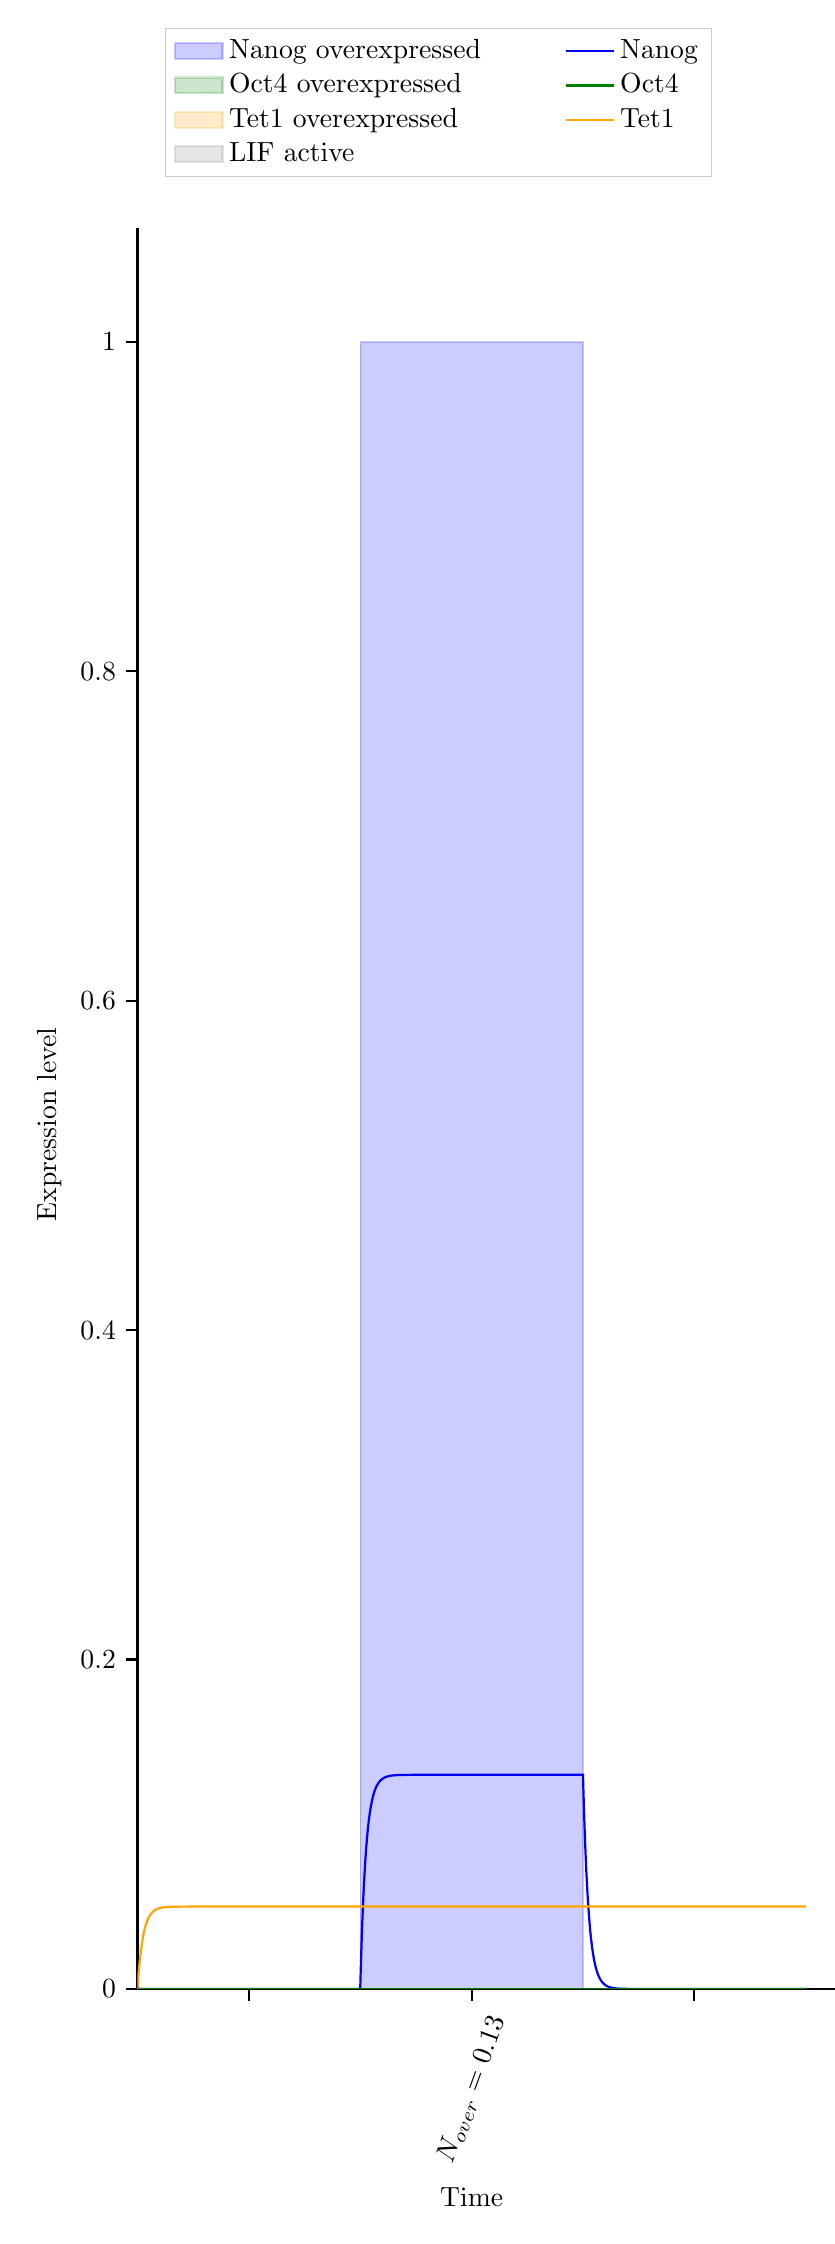
\begin{tikzpicture}[baseline]

\definecolor{darkgray176}{RGB}{176,176,176}
\definecolor{green}{RGB}{0,128,0}
\definecolor{lightgray204}{RGB}{204,204,204}
\definecolor{orange}{RGB}{255,165,0}

\begin{axis}[
 ytick={0,0.2,0.4,0.6,0.8,1},
 x tick label style = {rotate=70},
 y post scale=3, 
 transpose legend,
legend cell align={left},
legend style={fill opacity=0.8, draw opacity=1, text opacity=1, draw=lightgray204, anchor=south west,
    legend columns=4,
    /tikz/every even column/.append style={column sep=1.0cm},, at={(axis cs:5,1.1)}},
tick align=outside,
tick pos=left,
x grid style={darkgray176},
xlabel={Time},
xmin=0, xmax=120,
xtick style={color=black},
xtick={20,60,100},
xticklabels={,\(\displaystyle N_\text{over}=0.13\),},
y grid style={darkgray176},
ylabel={Expression level},
ymin=0, ymax=1.05,
ytick style={color=black}
]
\path [draw=blue, fill=blue, opacity=0.2]
(axis cs:40,0)
--(axis cs:40,1)
--(axis cs:80,1)
--(axis cs:80,0)
--cycle;
\addlegendimage{area legend, draw=blue, fill=blue, opacity=0.2}
\addlegendentry{Nanog overexpressed}
\addlegendimage{area legend, draw=green, fill=green, opacity=0.2}
\addlegendentry{Oct4 overexpressed}

\addlegendimage{area legend, draw=orange, fill=orange, opacity=0.2}
\addlegendentry{Tet1 overexpressed}

\addlegendimage{area legend, draw=gray, fill=gray, opacity=0.2}
\addlegendentry{LIF active}

\addplot [thick, blue]
table {%
0 0
0.0001 0
0.0011 0
0.0111 0
0.1111 0
0.2111 0
0.3111 0
0.4111 0
0.5111 0
0.6111 0
0.7111 0
0.8111 0
0.9111 0
1.0111 0
1.1111 0
1.2111 0
1.3111 0
1.4111 0
1.5111 0
1.6111 0
1.7111 0
1.8111 0
1.9111 0
2.0111 0
2.1111 0
2.2111 0
2.3111 0
2.4111 0
2.5111 0
2.6111 0
2.7111 0
2.8111 0
2.9111 0
3.0111 0
3.1111 0
3.2111 0
3.3111 0
3.4111 0
3.5111 0
3.6111 0
3.7111 0
3.8111 0
3.9111 0
4.0111 0
4.1111 0
4.2111 0
4.3111 0
4.4111 0
4.5111 0
4.6111 0
4.7111 0
4.8111 0
4.9111 0
5.0111 0
5.1111 0
5.2111 0
5.3111 0
5.4111 0
5.5111 0
5.6111 0
5.7111 0
5.8111 0
5.9111 0
6.0111 0
6.1111 0
6.21109999999999 0
6.31109999999999 0
6.41109999999999 0
6.51109999999999 0
6.61109999999999 0
6.71109999999999 0
6.81109999999999 0
6.91109999999999 0
7.01109999999999 0
7.11109999999999 0
7.21109999999999 0
7.31109999999999 0
7.41109999999999 0
7.51109999999999 0
7.61109999999999 0
7.71109999999999 0
7.81109999999999 0
7.91109999999999 0
8.01109999999999 0
8.11109999999999 0
8.21109999999999 0
8.31109999999999 0
8.41109999999999 0
8.51109999999999 0
8.61109999999999 0
8.71109999999999 0
8.81109999999999 0
8.91109999999999 0
9.01109999999998 0
9.11109999999998 0
9.21109999999998 0
9.31109999999998 0
9.41109999999998 0
9.51109999999998 0
9.61109999999998 0
9.71109999999998 0
9.81109999999998 0
9.91109999999998 0
10.0111 0
10.1111 0
10.2111 0
10.3111 0
10.4111 0
10.5111 0
10.6111 0
10.7111 0
10.8111 0
10.9111 0
11.0111 0
11.1111 0
11.2111 0
11.3111 0
11.4111 0
11.5111 0
11.6111 0
11.7111 0
11.8111 0
11.9111 0
12.0111 0
12.1111 0
12.2111 0
12.3111 0
12.4111 0
12.5111 0
12.6111 0
12.7111 0
12.8111 0
12.9111 0
13.0111 0
13.1111 0
13.2111 0
13.3111 0
13.4111 0
13.5111 0
13.6111 0
13.7111 0
13.8111 0
13.9111 0
14.0111 0
14.1111 0
14.2111 0
14.3111 0
14.4111 0
14.5111 0
14.6111 0
14.7111 0
14.8111 0
14.9111 0
15.0111 0
15.1111 0
15.2111 0
15.3111 0
15.4111 0
15.5111 0
15.6111 0
15.7111 0
15.8111 0
15.9111 0
16.0111 0
16.1111 0
16.2111 0
16.3111 0
16.4111 0
16.5111 0
16.6111 0
16.7111 0
16.8111 0
16.9111 0
17.0111 0
17.1111 0
17.2111 0
17.3111 0
17.4111 0
17.5111 0
17.6111 0
17.7111 0
17.8111 0
17.9111 0
18.0111 0
18.1111 0
18.2111 0
18.3111 0
18.4111 0
18.5111 0
18.6111 0
18.7111 0
18.8111 0
18.9111 0
19.0111 0
19.1111 0
19.2111 0
19.3111 0
19.4111 0
19.5111 0
19.6111 0
19.7111 0
19.8111 0
19.9111 0
20.0111 0
20.1111 0
20.2111 0
20.3111 0
20.4111 0
20.5111 0
20.6111 0
20.7111 0
20.8111 0
20.9111 0
21.0111 0
21.1111 0
21.2111 0
21.3111 0
21.4111 0
21.5111 0
21.6111 0
21.7111 0
21.8111 0
21.9111 0
22.0111 0
22.1111 0
22.2111 0
22.3111 0
22.4111000000001 0
22.5111000000001 0
22.6111000000001 0
22.7111000000001 0
22.8111000000001 0
22.9111000000001 0
23.0111000000001 0
23.1111000000001 0
23.2111000000001 0
23.3111000000001 0
23.4111000000001 0
23.5111000000001 0
23.6111000000001 0
23.7111000000001 0
23.8111000000001 0
23.9111000000001 0
24.0111000000001 0
24.1111000000001 0
24.2111000000001 0
24.3111000000001 0
24.4111000000001 0
24.5111000000001 0
24.6111000000001 0
24.7111000000001 0
24.8111000000001 0
24.9111000000001 0
25.0111000000001 0
25.1111000000001 0
25.2111000000001 0
25.3111000000001 0
25.4111000000001 0
25.5111000000001 0
25.6111000000001 0
25.7111000000001 0
25.8111000000001 0
25.9111000000001 0
26.0111000000001 0
26.1111000000001 0
26.2111000000001 0
26.3111000000001 0
26.4111000000001 0
26.5111000000001 0
26.6111000000001 0
26.7111000000001 0
26.8111000000001 0
26.9111000000001 0
27.0111000000001 0
27.1111000000001 0
27.2111000000001 0
27.3111000000001 0
27.4111000000001 0
27.5111000000001 0
27.6111000000001 0
27.7111000000001 0
27.8111000000001 0
27.9111000000001 0
28.0111000000001 0
28.1111000000001 0
28.2111000000001 0
28.3111000000001 0
28.4111000000001 0
28.5111000000001 0
28.6111000000001 0
28.7111000000001 0
28.8111000000001 0
28.9111000000001 0
29.0111000000001 0
29.1111000000001 0
29.2111000000001 0
29.3111000000001 0
29.4111000000002 0
29.5111000000002 0
29.6111000000002 0
29.7111000000002 0
29.8111000000002 0
29.9111000000002 0
30.0111000000002 0
30.1111000000002 0
30.2111000000002 0
30.3111000000002 0
30.4111000000002 0
30.5111000000002 0
30.6111000000002 0
30.7111000000002 0
30.8111000000002 0
30.9111000000002 0
31.0111000000002 0
31.1111000000002 0
31.2111000000002 0
31.3111000000002 0
31.4111000000002 0
31.5111000000002 0
31.6111000000002 0
31.7111000000002 0
31.8111000000002 0
31.9111000000002 0
32.0111000000002 0
32.1111000000002 0
32.2111000000002 0
32.3111000000002 0
32.4111000000002 0
32.5111000000002 0
32.6111000000002 0
32.7111000000002 0
32.8111000000002 0
32.9111000000002 0
33.0111000000002 0
33.1111000000002 0
33.2111000000002 0
33.3111000000002 0
33.4111000000002 0
33.5111000000002 0
33.6111000000002 0
33.7111000000002 0
33.8111000000002 0
33.9111000000002 0
34.0111000000002 0
34.1111000000002 0
34.2111000000002 0
34.3111000000002 0
34.4111000000002 0
34.5111000000002 0
34.6111000000002 0
34.7111000000002 0
34.8111000000002 0
34.9111000000002 0
35.0111000000002 0
35.1111000000002 0
35.2111000000002 0
35.3111000000002 0
35.4111000000002 0
35.5111000000002 0
35.6111000000002 0
35.7111000000002 0
35.8111000000002 0
35.9111000000002 0
36.0111000000002 0
36.1111000000002 0
36.2111000000002 0
36.3111000000002 0
36.4111000000002 0
36.5111000000002 0
36.6111000000002 0
36.7111000000003 0
36.8111000000003 0
36.9111000000003 0
37.0111000000003 0
37.1111000000003 0
37.2111000000003 0
37.3111000000003 0
37.4111000000003 0
37.5111000000003 0
37.6111000000003 0
37.7111000000003 0
37.8111000000003 0
37.9111000000003 0
38.0111000000003 0
38.1111000000003 0
38.2111000000003 0
38.3111000000003 0
38.4111000000003 0
38.5111000000003 0
38.6111000000003 0
38.7111000000003 0
38.8111000000003 0
38.9111000000003 0
39.0111000000003 0
39.1111000000003 0
39.2111000000003 0
39.3111000000003 0
39.4111000000003 0
39.5111000000003 0
39.6111000000003 0
39.7111000000003 0
39.8111000000003 0
39.9111000000003 0
40 0
40 0
40.0075414781297 0.000976704629483531
40.0829562594269 0.0103491173707178
40.1829562594269 0.0217354042604158
40.2829562594269 0.0320381426940927
40.3829562594269 0.0413604459401846
40.4829562594269 0.0497956147422988
40.5829562594269 0.0574280711044097
40.6829562594269 0.0643342032146439
40.7829562594269 0.0705831299639372
40.8829562594269 0.0762373927111218
40.9829562594269 0.0813535812178627
41.0829562594269 0.0859829000180088
41.1829562594269 0.0901716808897749
41.2829562594269 0.0939618465597478
41.3829562594269 0.0973913302796217
41.4829562594269 0.100494455474929
41.5829562594269 0.103302279265415
41.6829562594269 0.105842903295134
41.7829562594269 0.10814175498314
41.8829562594269 0.110221842009647
41.9829562594269 0.112103982584621
42.0829562594269 0.11380701380342
42.1829562594269 0.115347980174779
42.2829562594269 0.116742304207978
42.3829562594269 0.118003940766498
42.4829562594269 0.119145516732985
42.5829562594269 0.120178457383331
42.6829562594269 0.121113100734683
42.7829562594269 0.121958801011782
42.8829562594269 0.122724022267196
42.9829562594269 0.123416423092399
43.0829562594269 0.124042933267527
43.1829562594269 0.12460982311695
43.2829562594269 0.125122766264781
43.3829562594269 0.125586896418416
43.4829562594269 0.126006858748402
43.5829562594269 0.126386856378864
43.6829562594269 0.126730692453784
43.7829562594269 0.127041808200144
43.8829562594269 0.127323317368883
43.9829562594269 0.127578037398363
44.0829562594269 0.127808517612235
44.1829562594269 0.128017064733932
44.2829562594269 0.128205765973128
44.3829562594269 0.12837650991524
44.4829562594269 0.128531005423016
44.582956259427 0.128670798739416
44.682956259427 0.128797288962928
44.782956259427 0.128911742050214
44.882956259427 0.129015303486235
44.982956259427 0.129109009748643
45.082956259427 0.129193798681202
45.182956259427 0.129270518880042
45.282956259427 0.129339938186694
45.382956259427 0.129402751372908
45.482956259427 0.129459587094159
45.582956259427 0.129511014181445
45.682956259427 0.129557547334337
45.782956259427 0.129599652272267
45.882956259427 0.129637750395602
45.982956259427 0.129672223003164
46.082956259427 0.129703415108394
46.182956259427 0.129731638892363
46.282956259427 0.129757176828185
46.382956259427 0.129780284508103
46.482956259427 0.129801193201544
46.582956259427 0.129820112169738
46.682956259427 0.129837230760076
46.782956259427 0.129852720301163
46.882956259427 0.129866735817532
46.982956259427 0.129879417581179
47.082956259427 0.129890892515458
47.182956259427 0.129901275465366
47.282956259427 0.129910670346955
47.382956259427 0.129919171187359
47.482956259427 0.129926863065843
47.582956259427 0.129933822965312
47.682956259427 0.12994012054278
47.782956259427 0.129945818826518
47.882956259427 0.129950974846864
47.982956259427 0.129955640207003
48.082956259427 0.129959861599427
48.182956259427 0.129963681273249
48.282956259427 0.12996713745705
48.382956259427 0.129970264741477
48.482956259427 0.129973094425445
48.582956259427 0.129975654829381
48.682956259427 0.129977971578668
48.782956259427 0.129980067860112
48.882956259427 0.129981964654002
48.982956259427 0.129983680944088
49.082956259427 0.129985233907579
49.182956259427 0.129986639087055
49.282956259427 0.129987910546024
49.382956259427 0.129989061009676
49.482956259427 0.129990101992236
49.582956259427 0.129991043912208
49.682956259427 0.129991896196644
49.782956259427 0.129992667375493
49.882956259427 0.129993365166971
49.982956259427 0.129993996554811
50.082956259427 0.129994567858154
50.182956259427 0.129995084794796
50.282956259427 0.129995552538413
50.382956259427 0.129995975770339
50.482956259427 0.129996358726423
50.582956259427 0.129996705239417
50.682956259427 0.12999701877734
50.782956259427 0.129997302478185
50.882956259427 0.129997559181325
50.982956259427 0.129997791455932
51.082956259427 0.129998001626687
51.182956259427 0.12999819179705
51.282956259427 0.129998363870311
51.382956259427 0.129998519568636
51.482956259427 0.129998660450307
51.582956259427 0.129998787925314
51.6829562594271 0.12999890326947
51.7829562594271 0.129999007637179
51.8829562594271 0.129999102072987
51.9829562594271 0.12999918752204
52.0829562594271 0.12999926483954
52.1829562594271 0.129999334799307
52.2829562594271 0.129999398101522
52.3829562594271 0.129999455379735
52.4829562594271 0.129999507207206
52.5829562594271 0.12999955410264
52.6829562594271 0.129999596535384
52.7829562594271 0.129999634930119
52.8829562594271 0.129999669671111
52.9829562594271 0.129999701106061
53.0829562594271 0.12999972954958
53.1829562594271 0.12999975528634
53.2829562594271 0.129999778573924
53.3829562594271 0.129999799645401
53.4829562594271 0.129999818711662
53.5829562594271 0.129999835963528
53.6829562594271 0.129999851573662
53.7829562594271 0.129999865698296
53.8829562594271 0.129999878478793
53.9829562594271 0.129999890043064
54.0829562594271 0.12999990050685
54.1829562594271 0.129999909974875
54.2829562594271 0.129999918541899
54.3829562594271 0.129999926293662
54.4829562594271 0.129999933307747
54.5829562594271 0.129999939654354
54.6829562594271 0.129999945397002
54.7829562594271 0.129999950593164
54.8829562594271 0.129999955294846
54.9829562594271 0.129999959549104
55.0829562594271 0.129999963398516
55.1829562594271 0.129999966881607
55.2829562594271 0.129999970033239
55.3829562594271 0.129999972884953
55.4829562594271 0.129999975465291
55.5829562594271 0.129999977800077
55.6829562594271 0.129999979912679
55.7829562594271 0.129999981824241
55.8829562594271 0.129999983553893
55.9829562594271 0.129999985118947
56.0829562594271 0.129999986535066
56.1829562594271 0.129999987816424
56.2829562594271 0.129999988975845
56.3829562594271 0.129999990024932
56.4829562594271 0.129999990974185
56.5829562594271 0.129999991833105
56.6829562594271 0.129999992610288
56.7829562594271 0.129999993313512
56.8829562594271 0.129999993949815
56.9829562594271 0.129999994525566
57.0829562594271 0.129999995046528
57.1829562594271 0.129999995517913
57.2829562594271 0.12999999594444
57.3829562594271 0.129999996330377
57.4829562594271 0.129999996679588
57.5829562594271 0.129999996995567
57.6829562594271 0.129999997281477
57.7829562594271 0.129999997540178
57.8829562594271 0.129999997774261
57.9829562594271 0.129999997986068
58.0829562594271 0.129999998177719
58.1829562594271 0.129999998351132
58.2829562594271 0.129999998508043
58.3829562594271 0.129999998650021
58.4829562594271 0.129999998778489
58.5829562594271 0.129999998894731
58.6829562594272 0.129999998999911
58.7829562594272 0.129999999095082
58.8829562594272 0.129999999181197
58.9829562594272 0.129999999259116
59.0829562594272 0.12999999932962
59.1829562594272 0.129999999393415
59.2829562594272 0.12999999945114
59.3829562594272 0.129999999503371
59.4829562594272 0.129999999550631
59.5829562594272 0.129999999593394
59.6829562594272 0.129999999632088
59.7829562594272 0.129999999667099
59.8829562594272 0.129999999698779
59.9829562594272 0.129999999727444
60.0829562594272 0.129999999753381
60.1829562594272 0.12999999977685
60.2829562594272 0.129999999798086
60.3829562594272 0.1299999998173
60.4829562594272 0.129999999834686
60.5829562594272 0.129999999850418
60.6829562594272 0.129999999864653
60.7829562594272 0.129999999877533
60.8829562594272 0.129999999889187
60.9829562594272 0.129999999899732
61.0829562594272 0.129999999909274
61.1829562594272 0.129999999917908
61.2829562594272 0.12999999992572
61.3829562594272 0.129999999932789
61.4829562594272 0.129999999939185
61.5829562594272 0.129999999944972
61.6829562594272 0.129999999950209
61.7829562594272 0.129999999954947
61.8829562594272 0.129999999959234
61.9829562594272 0.129999999963114
62.0829562594272 0.129999999966624
62.1829562594272 0.1299999999698
62.2829562594272 0.129999999972674
62.3829562594272 0.129999999975274
62.4829562594272 0.129999999977627
62.5829562594272 0.129999999979756
62.6829562594272 0.129999999981683
62.7829562594272 0.129999999983426
62.8829562594272 0.129999999985003
62.9829562594272 0.12999999998643
63.0829562594272 0.129999999987722
63.1829562594272 0.12999999998889
63.2829562594272 0.129999999989947
63.3829562594272 0.129999999990904
63.4829562594272 0.12999999999177
63.5829562594272 0.129999999992553
63.6829562594272 0.129999999993261
63.7829562594272 0.129999999993903
63.8829562594272 0.129999999994483
63.9829562594272 0.129999999995008
64.0829562594272 0.129999999995483
64.1829562594272 0.129999999995913
64.2829562594272 0.129999999996302
64.3829562594272 0.129999999996654
64.4829562594272 0.129999999996972
64.5829562594272 0.12999999999726
64.6829562594272 0.129999999997521
64.7829562594272 0.129999999997757
64.8829562594272 0.12999999999797
64.9829562594272 0.129999999998164
65.0829562594272 0.129999999998338
65.1829562594272 0.129999999998496
65.2829562594272 0.12999999999864
65.3829562594271 0.129999999998769
65.4829562594271 0.129999999998886
65.5829562594271 0.129999999998992
65.6829562594271 0.129999999999088
65.7829562594271 0.129999999999175
65.8829562594271 0.129999999999253
65.9829562594271 0.129999999999324
66.0829562594271 0.129999999999389
66.1829562594271 0.129999999999447
66.2829562594271 0.1299999999995
66.3829562594271 0.129999999999547
66.4829562594271 0.12999999999959
66.5829562594271 0.129999999999629
66.6829562594271 0.129999999999665
66.7829562594271 0.129999999999696
66.8829562594271 0.129999999999725
66.9829562594271 0.129999999999751
67.082956259427 0.129999999999775
67.182956259427 0.129999999999797
67.282956259427 0.129999999999816
67.382956259427 0.129999999999833
67.482956259427 0.129999999999849
67.582956259427 0.129999999999864
67.682956259427 0.129999999999877
67.782956259427 0.129999999999888
67.882956259427 0.129999999999899
67.982956259427 0.129999999999909
68.082956259427 0.129999999999917
68.182956259427 0.129999999999925
68.282956259427 0.129999999999932
68.382956259427 0.129999999999939
68.482956259427 0.129999999999945
68.582956259427 0.12999999999995
68.682956259427 0.129999999999955
68.782956259427 0.129999999999959
68.8829562594269 0.129999999999963
68.9829562594269 0.129999999999966
69.0829562594269 0.12999999999997
69.1829562594269 0.129999999999972
69.2829562594269 0.129999999999975
69.3829562594269 0.129999999999977
69.4829562594269 0.12999999999998
69.5829562594269 0.129999999999982
69.6829562594269 0.129999999999983
69.7829562594269 0.129999999999985
69.8829562594269 0.129999999999986
69.9829562594269 0.129999999999988
70.0829562594269 0.129999999999989
70.1829562594269 0.12999999999999
70.2829562594269 0.129999999999991
70.3829562594269 0.129999999999992
70.4829562594269 0.129999999999992
70.5829562594269 0.129999999999993
70.6829562594268 0.129999999999994
70.7829562594268 0.129999999999994
70.8829562594268 0.129999999999995
70.9829562594268 0.129999999999995
71.0829562594268 0.129999999999996
71.1829562594268 0.129999999999996
71.2829562594268 0.129999999999997
71.3829562594268 0.129999999999997
71.4829562594268 0.129999999999997
71.5829562594268 0.129999999999997
71.6829562594268 0.129999999999998
71.7829562594268 0.129999999999998
71.8829562594268 0.129999999999998
71.9829562594268 0.129999999999998
72.0829562594268 0.129999999999998
72.1829562594268 0.129999999999999
72.2829562594268 0.129999999999999
72.3829562594267 0.129999999999999
72.4829562594267 0.129999999999999
72.5829562594267 0.129999999999999
72.6829562594267 0.129999999999999
72.7829562594267 0.129999999999999
72.8829562594267 0.129999999999999
72.9829562594267 0.129999999999999
73.0829562594267 0.129999999999999
73.1829562594267 0.13
73.2829562594267 0.13
73.3829562594267 0.13
73.4829562594267 0.13
73.5829562594267 0.13
73.6829562594267 0.13
73.7829562594267 0.13
73.8829562594267 0.13
73.9829562594267 0.13
74.0829562594267 0.13
74.1829562594266 0.13
74.2829562594266 0.13
74.3829562594266 0.13
74.4829562594266 0.13
74.5829562594266 0.13
74.6829562594266 0.13
74.7829562594266 0.13
74.8829562594266 0.13
74.9829562594266 0.13
75.0829562594266 0.13
75.1829562594266 0.13
75.2829562594266 0.13
75.3829562594266 0.13
75.4829562594266 0.13
75.5829562594266 0.13
75.6829562594266 0.13
75.7829562594266 0.13
75.8829562594265 0.13
75.9829562594265 0.13
76.0829562594265 0.13
76.1829562594265 0.13
76.2829562594265 0.13
76.3829562594265 0.13
76.4829562594265 0.13
76.5829562594265 0.13
76.6829562594265 0.13
76.7829562594265 0.13
76.8829562594265 0.13
76.9829562594265 0.13
77.0829562594265 0.13
77.1829562594265 0.13
77.2829562594265 0.13
77.3829562594265 0.13
77.4829562594265 0.13
77.5829562594265 0.13
77.6829562594264 0.13
77.7829562594264 0.13
77.8829562594264 0.13
77.9829562594264 0.13
78.0829562594264 0.13
78.1829562594264 0.13
78.2829562594264 0.13
78.3829562594264 0.13
78.4829562594264 0.13
78.5829562594264 0.13
78.6829562594264 0.13
78.7829562594264 0.13
78.8829562594264 0.13
78.9829562594264 0.13
79.0829562594264 0.13
79.1829562594264 0.13
79.2829562594264 0.13
79.3829562594264 0.13
79.4829562594263 0.13
79.5829562594263 0.13
79.6829562594263 0.13
79.7829562594263 0.13
79.8829562594263 0.13
79.9829562594263 0.13
80 0.13
80 0.13
80.1 0.117628864383334
80.2 0.106434997970098
80.3 0.0963063687835778
80.4 0.0871416060991909
80.5 0.0788489858922126
80.6 0.0713455128329115
80.7 0.0645560896413997
80.8 0.0584127654888197
80.8999999999999 0.0528540559226143
80.9999999999999 0.0478243275094643
81.0999999999999 0.0432732410371917
81.1999999999999 0.0391552477030088
81.2999999999999 0.0354291332457929
81.3999999999999 0.0320576054599111
81.4999999999999 0.0290069209622947
81.5999999999999 0.0262465474773219
81.6999999999999 0.0237488582595434
81.7999999999999 0.0214888555959296
81.8999999999999 0.0194439206203588
81.9999999999999 0.0175935869364039
82.0999999999999 0.0159193357827588
82.1999999999999 0.014404410691253
82.2999999999999 0.0130336497824865
82.3999999999999 0.011793334020646
82.4999999999999 0.010671049908784
82.5999999999999 0.00965556525037037
82.6999999999998 0.00873671673369422
82.7999999999998 0.00790530821402555
82.8999999999998 0.00715301867550822
82.9999999999998 0.00647231895163701
83.0999999999998 0.00585639637082917
83.1999999999998 0.0052990865729178
83.2999999999998 0.0047948118141638
83.3999999999998 0.00433852514332216
83.4999999999998 0.0039256598900579
83.5999999999998 0.00355208396017473
83.6999999999998 0.00321405848022777
83.7999999999998 0.00290820037762166
83.8999999999998 0.00263144852168323
83.9999999999998 0.00238103308683693
84.0999999999998 0.00215444783125979
84.1999999999998 0.00194942501357097
84.2999999999998 0.00176391269651399
84.3999999999997 0.00159605421047911
84.4999999999997 0.00144416957132998
84.5999999999997 0.00130673866655778
84.6999999999997 0.00118238604148449
84.7999999999997 0.0010698671332502
84.8999999999997 0.000968055814809803
84.9999999999997 0.000875933124275078
85.0999999999997 0.000792577066801717
85.1999999999997 0.000717153386955076
85.2999999999997 0.000648907219201441
85.3999999999997 0.000587155532960097
85.4999999999997 0.00053128029660375
85.5999999999997 0.000480722291990307
85.6999999999997 0.000434975517619795
85.7999999999997 0.000393582124401303
85.8999999999997 0.000356127833345426
85.9999999999997 0.00032223778932092
86.0999999999997 0.000291572809378584
86.1999999999996 0.000263825988094316
86.2999999999996 0.000238719625956503
86.3999999999996 0.000216002450055983
86.4999999999996 0.000195447099262331
86.5999999999996 0.000176847848717268
86.6999999999996 0.000160018550871137
86.7999999999996 0.000144790772455682
86.8999999999996 0.000131012108747289
86.9999999999996 0.000118544658249304
87.0999999999996 0.000107263642527508
87.1999999999996 9.70561573856202e-05
87.2999999999996 8.78200428821587e-05
87.3999999999996 7.94628608794156e-05
87.4999999999996 7.19009698915116e-05
87.5999999999996 6.50586879722985e-05
87.6999999999996 5.88675352650088e-05
87.7999999999996 5.32655486328373e-05
87.8999999999996 4.81966615110454e-05
87.9999999999995 4.36101427739401e-05
88.0999999999995 3.94600890007203e-05
88.1999999999995 3.57049650586155e-05
88.2999999999995 3.23071884053197e-05
88.3999999999995 2.92327529502782e-05
88.4999999999995 2.6450888710306e-05
88.5999999999995 2.39337538532558e-05
88.6999999999995 2.16561560476055e-05
88.7999999999995 1.95953003291393e-05
88.8999999999995 1.77305609612848e-05
88.9999999999995 1.60432750058108e-05
89.0999999999995 1.45165555378697e-05
89.1999999999995 1.31351226359785e-05
89.2999999999995 1.18851504554306e-05
89.3999999999995 1.07541288545951e-05
89.4999999999995 9.73073818921591e-06
89.5999999999995 8.80473602160775e-06
89.6999999999994 7.96685461089811e-06
89.7999999999994 7.2087081583621e-06
89.8999999999994 6.52270887953084e-06
89.9999999999994 5.90199106309462e-06
90.0999999999994 5.34034235655698e-06
90.1999999999994 4.83214159092319e-06
90.2999999999994 4.37230252215209e-06
90.3999999999994 3.95622292631644e-06
90.4999999999994 3.57973853899934e-06
90.5999999999994 3.23908137793652e-06
90.6999999999994 2.93084203178367e-06
90.7999999999994 2.65193553758197e-06
90.8999999999994 2.39957050541211e-06
90.9999999999994 2.17122118122591e-06
91.0999999999994 1.96460216825112e-06
91.1999999999994 1.77764555397242e-06
91.2999999999994 1.60848021376814e-06
91.3999999999994 1.45541308406622e-06
91.4999999999993 1.31691221759504e-06
91.5999999999993 1.19159145114033e-06
91.6999999999993 1.07819653235789e-06
91.7999999999993 9.75592566794673e-07
91.8999999999993 8.82752659483687e-07
91.9999999999993 7.98747637434108e-07
92.0999999999993 7.22736750155732e-07
92.1999999999993 6.5395925514554e-07
92.2999999999993 5.91726804121083e-07
92.3999999999993 5.35416553799558e-07
92.4999999999993 4.84464932272925e-07
92.5999999999993 4.38361998590869e-07
92.6999999999993 3.96646339100405e-07
92.7999999999993 3.5890044946298e-07
92.8999999999993 3.24746556130758e-07
92.9999999999993 2.93842835461997e-07
93.0999999999993 2.65879992635182e-07
93.1999999999992 2.40578166122505e-07
93.2999999999992 2.17684126741656e-07
93.3999999999992 1.96968743253067e-07
93.4999999999992 1.78224689137468e-07
93.5999999999992 1.61264367602408e-07
93.6999999999992 1.45918034050521e-07
93.7999999999992 1.3203209721855e-07
93.8999999999992 1.19467581984369e-07
93.9999999999992 1.08098738457263e-07
94.0999999999992 9.78117834307606e-08
94.1999999999992 8.8503761602069e-08
94.2999999999992 8.00815151608054e-08
94.3999999999992 7.24607514343253e-08
94.4999999999992 6.55651992583286e-08
94.5999999999992 5.9325845629417e-08
94.6999999999992 5.36802449997638e-08
94.7999999999992 4.85718943010874e-08
94.8999999999992 4.39496674429557e-08
94.9999999999991 3.97673036256928e-08
95.0999999999991 3.59829443467499e-08
95.1999999999991 3.25587144667454e-08
95.2999999999991 2.94603431423422e-08
95.3999999999991 2.66568208321312e-08
95.4999999999991 2.412008894272e-08
95.5999999999991 2.18247590089012e-08
95.6999999999991 1.97478585973615e-08
95.7999999999991 1.78686013908484e-08
95.8999999999991 1.61681791517227e-08
95.9999999999991 1.46295734827957e-08
96.0999999999991 1.32373855014907e-08
96.1999999999991 1.1977681722652e-08
96.2999999999991 1.08378546075429e-08
96.3999999999991 9.80649638336118e-09
96.4999999999991 8.87328487041575e-09
96.5999999999991 8.02888017428326e-09
96.6999999999991 7.26483120900619e-09
96.799999999999 6.57349111578463e-09
96.899999999999 5.9479407306437e-09
96.999999999999 5.38191933511536e-09
97.099999999999 4.86976199686406e-09
97.199999999999 4.40634287314028e-09
97.299999999999 3.98702390962375e-09
97.399999999999 3.60760842121725e-09
97.499999999999 3.26429909021183e-09
97.599999999999 2.95365996145514e-09
97.699999999999 2.67258205415761e-09
97.799999999999 2.41825224616799e-09
97.899999999999 2.18812511930144e-09
97.999999999999 1.97989748393904e-09
98.099999999999 1.79148532793207e-09
98.199999999999 1.62100295910811e-09
98.299999999999 1.46674413263009e-09
98.399999999999 1.32716497432458e-09
98.4999999999989 1.20086852907028e-09
98.5999999999989 1.08659077960171e-09
98.6999999999989 9.8318799579962e-10
98.7999999999989 8.89625287855657e-10
98.8999999999989 8.04966248747366e-10
98.9999999999989 7.28363582362039e-10
99.0999999999989 6.59050623472489e-10
99.1999999999989 5.96333664693824e-10
99.2999999999989 5.39585013626819e-10
99.3999999999989 4.8823671070145e-10
99.4999999999989 4.41774844846661e-10
99.5999999999989 3.99734410095664e-10
99.6999999999989 3.6169465164996e-10
99.7999999999989 3.27274854823926e-10
99.8999999999989 2.961305347243e-10
99.9999999999989 2.67949988529606e-10
100.099999999999 2.42451175863577e-10
100.199999999999 2.19378896040281e-10
100.299999999999 1.98502233929906e-10
100.399999999999 1.79612248882536e-10
100.499999999999 1.62519883579919e-10
100.599999999999 1.47054071886289e-10
100.699999999999 1.33060026760995e-10
100.799999999999 1.20397691097783e-10
100.899999999999 1.08940335986213e-10
100.999999999999 9.85732923661315e-11
101.099999999999 8.91928033811878e-11
101.199999999999 8.07049859453471e-11
101.299999999999 7.30248911294162e-11
101.399999999999 6.60756539636141e-11
101.499999999999 5.97877241471236e-11
101.599999999999 5.40981699653091e-11
101.699999999999 4.89500484479684e-11
101.799999999999 4.42918354649516e-11
101.899999999999 4.00769100553518e-11
101.999999999999 3.6263087829262e-11
102.099999999999 3.28121987722245e-11
102.199999999999 2.96897052268999e-11
102.299999999999 2.6864356228586e-11
102.399999999999 2.43078747350609e-11
102.499999999999 2.19946746204427e-11
102.599999999999 1.99016046006431e-11
102.699999999999 1.80077165275368e-11
102.799999999999 1.6294055732855e-11
102.899999999999 1.47434713234961e-11
102.999999999999 1.33404445296238e-11
103.099999999999 1.20709333876039e-11
103.199999999999 1.09222322033132e-11
103.299999999999 9.88284438928318e-12
103.399999999999 8.94236740298911e-12
103.499999999999 8.09138863470887e-12
103.599999999999 7.32139120296169e-12
103.699999999999 6.62466871469627e-12
103.799999999999 5.99424813711941e-12
103.899999999999 5.42382000924055e-12
103.999999999999 4.90767529466592e-12
104.099999999999 4.44064824364382e-12
104.199999999999 4.01806469250515e-12
104.299999999999 3.6356952830627e-12
104.399999999999 3.28971313377315e-12
104.499999999999 2.97665553902057e-12
104.599999999999 2.693389313195e-12
104.699999999999 2.43707943271797e-12
104.799999999999 2.20516066217381e-12
104.899999999999 1.99531188057158e-12
104.999999999999 1.80543285078623e-12
105.099999999999 1.63362319967961e-12
105.199999999999 1.47816339852755e-12
105.299999999999 1.3374975533985e-12
105.399999999999 1.21021783324425e-12
105.499999999999 1.0950503798537e-12
105.599999999999 9.90842558651762e-13
105.699999999999 8.9655142274526e-13
105.799999999999 8.11233274759902e-13
105.899999999999 7.3403422199985e-13
105.999999999999 6.64181630402665e-13
106.099999999999 6.00976391757975e-13
106.199999999999 5.43785926797571e-13
106.299999999999 4.92037854129516e-13
106.399999999998 4.45214261652827e-13
106.499999999998 4.02846523119127e-13
106.599999999998 3.64510607963673e-13
106.699999999998 3.29822837464965e-13
106.799999999998 2.98436044759176e-13
106.899999999998 2.70036100277505e-13
106.999999999998 2.443387678319e-13
107.099999999998 2.21086859883765e-13
107.199999999998 2.00047663524651e-13
107.299999999998 1.81010611407261e-13
107.399999999998 1.63785174316686e-13
107.499999999998 1.48198954289986e-13
107.599999999998 1.34095959199451e-13
107.699999999998 1.21335041530964e-13
107.799999999998 1.09788485732246e-13
107.899999999998 9.93407299926919e-14
107.999999999998 8.98872096619366e-14
108.099999999998 8.13333107316942e-14
108.199999999998 7.35934229069694e-14
108.299999999998 6.65900827894558e-14
108.399999999998 6.02531985978144e-14
108.499999999998 5.45193486655724e-14
108.599999999998 4.93311466957716e-14
108.699999999998 4.46366674196252e-14
108.799999999998 4.03889269109775e-14
108.899999999998 3.65454123553828e-14
108.999999999998 3.30676565675719e-14
109.099999999998 2.99208529989352e-14
109.199999999998 2.70735073818878e-14
109.299999999998 2.4497122524656e-14
109.399999999998 2.21659131018052e-14
109.499999999998 2.00565475860385e-14
109.599999999998 1.81479147384309e-14
109.699999999998 1.64209123200553e-14
109.799999999998 1.4858255910357e-14
109.899999999998 1.34443059188635e-14
109.999999999998 1.2164911058908e-14
110.099999999998 1.1007266716797e-14
110.199999999998 9.9597867989331e-15
110.299999999998 9.01198777429709e-15
110.399999999998 8.15438375174659e-15
110.499999999998 7.37839154202971e-15
110.599999999998 6.6762447543427e-15
110.699999999998 6.04091606768094e-15
110.799999999998 5.46604689904881e-15
110.899999999998 4.94588376462427e-15
110.999999999998 4.4752206969594e-15
111.099999999998 4.04934714190867e-15
111.199999999998 3.66400081382012e-15
111.299999999998 3.31532503714825e-15
111.399999999998 2.9998301475491e-15
111.499999999998 2.71435856614685e-15
111.599999999998 2.4560531974233e-15
111.699999999998 2.22232883444584e-15
111.799999999998 2.01084628524771e-15
111.899999999998 1.81948896140872e-15
111.999999999998 1.64634169452707e-15
112.099999999998 1.48967156857041e-15
112.199999999998 1.34791057626983e-15
112.299999999998 1.21963992597619e-15
112.399999999998 1.10357584191656e-15
112.499999999998 9.98556715734822e-16
112.599999999998 9.03531480724914e-16
112.699999999998 8.17549092402029e-16
112.799999999998 7.39749010129816e-16
112.899999999998 6.69352584540506e-16
112.999999999998 6.05655264550379e-16
113.099999999998 5.4801954597576e-16
113.199999999998 4.95868591176915e-16
113.299999999998 4.48680455873109e-16
113.399999999998 4.0598286534885e-16
113.499999999998 3.67348487769824e-16
113.599999999998 3.32390657302304e-16
113.699999999998 3.00759504231538e-16
113.799999999998 2.7213845334808e-16
113.899999999998 2.46241055556704e-16
113.999999999998 2.22808120997604e-16
114.099999999998 2.01605124987174e-16
114.199999999998 1.82419860816165e-16
114.299999999998 1.65060315913626e-16
114.399999999998 1.4935275012057e-16
114.499999999998 1.35139956840081e-16
114.599999999998 1.22279689660858e-16
114.699999999998 1.10643238707332e-16
114.799999999998 1.00114142467982e-16
114.899999999998 9.05870222093847e-17
114.999999999998 8.19665273104445e-17
115.099999999998 7.41663809613317e-17
115.199999999998 6.71085166761782e-17
115.299999999998 6.07222969774529e-17
115.399999999998 5.49438064323487e-17
115.499999999998 4.97152119656531e-17
115.599999999998 4.49841840468963e-17
115.699999999998 4.07033729588254e-17
115.799999999998 3.68299349055226e-17
115.899999999998 3.33251032172979e-17
115.999999999998 3.01538003608319e-17
116.099999999998 2.7284286871434e-17
116.199999999998 2.46878436938146e-17
116.299999999998 2.23384847521282e-17
116.399999999998 2.02126968725943e-17
116.499999999998 1.82892044557526e-17
116.599999999998 1.65487565431137e-17
116.699999999998 1.4973934147098e-17
116.799999999998 1.35489759159536e-17
116.899999999998 1.2259620388852e-17
116.999999999998 1.10929632623956e-17
117.099999999998 1.00373282400126e-17
117.199999999998 9.08215017165731e-18
117.299999999998 8.21786931423809e-18
117.399999999998 7.43583565449595e-18
117.499999999998 6.72822233676511e-18
117.599999999998 6.08794732917124e-18
117.699999999998 5.50860254427665e-18
117.799999999998 4.98438970478774e-18
117.899999999998 4.51006231244741e-18
117.999999999998 4.0808731393174e-18
118.099999999998 3.69252671592583e-18
118.199999999998 3.34113634076521e-18
118.299999999998 3.02318518087769e-18
118.399999999998 2.73549107420897e-18
118.499999999998 2.47517468146114e-18
118.599999999998 2.23963066869734e-18
118.699999999998 2.02650163228427e-18
118.799999999998 1.83365450520439e-18
118.899999999998 1.65915920860444e-18
118.999999999998 1.50126933491763e-18
119.099999999998 1.35840466922987e-18
119.199999999998 1.22913537395791e-18
119.299999999998 1.11216767855426e-18
119.399999999998 1.00633093101682e-18
119.499999999998 9.10565881610242e-19
119.599999999998 8.23914081538632e-19
119.699999999998 7.455082904679e-19
119.799999999998 6.74563796893075e-19
119.899999999998 6.10370564481864e-19
119.999999999998 5.52286125792433e-19
120 5.52286125791177e-19
};
\addlegendentry{Nanog}
\addplot [thick, green]
table {%
0 0
0.0001 0
0.0011 0
0.0111 0
0.1111 0
0.2111 0
0.3111 0
0.4111 0
0.5111 0
0.6111 0
0.7111 0
0.8111 0
0.9111 0
1.0111 0
1.1111 0
1.2111 0
1.3111 0
1.4111 0
1.5111 0
1.6111 0
1.7111 0
1.8111 0
1.9111 0
2.0111 0
2.1111 0
2.2111 0
2.3111 0
2.4111 0
2.5111 0
2.6111 0
2.7111 0
2.8111 0
2.9111 0
3.0111 0
3.1111 0
3.2111 0
3.3111 0
3.4111 0
3.5111 0
3.6111 0
3.7111 0
3.8111 0
3.9111 0
4.0111 0
4.1111 0
4.2111 0
4.3111 0
4.4111 0
4.5111 0
4.6111 0
4.7111 0
4.8111 0
4.9111 0
5.0111 0
5.1111 0
5.2111 0
5.3111 0
5.4111 0
5.5111 0
5.6111 0
5.7111 0
5.8111 0
5.9111 0
6.0111 0
6.1111 0
6.21109999999999 0
6.31109999999999 0
6.41109999999999 0
6.51109999999999 0
6.61109999999999 0
6.71109999999999 0
6.81109999999999 0
6.91109999999999 0
7.01109999999999 0
7.11109999999999 0
7.21109999999999 0
7.31109999999999 0
7.41109999999999 0
7.51109999999999 0
7.61109999999999 0
7.71109999999999 0
7.81109999999999 0
7.91109999999999 0
8.01109999999999 0
8.11109999999999 0
8.21109999999999 0
8.31109999999999 0
8.41109999999999 0
8.51109999999999 0
8.61109999999999 0
8.71109999999999 0
8.81109999999999 0
8.91109999999999 0
9.01109999999998 0
9.11109999999998 0
9.21109999999998 0
9.31109999999998 0
9.41109999999998 0
9.51109999999998 0
9.61109999999998 0
9.71109999999998 0
9.81109999999998 0
9.91109999999998 0
10.0111 0
10.1111 0
10.2111 0
10.3111 0
10.4111 0
10.5111 0
10.6111 0
10.7111 0
10.8111 0
10.9111 0
11.0111 0
11.1111 0
11.2111 0
11.3111 0
11.4111 0
11.5111 0
11.6111 0
11.7111 0
11.8111 0
11.9111 0
12.0111 0
12.1111 0
12.2111 0
12.3111 0
12.4111 0
12.5111 0
12.6111 0
12.7111 0
12.8111 0
12.9111 0
13.0111 0
13.1111 0
13.2111 0
13.3111 0
13.4111 0
13.5111 0
13.6111 0
13.7111 0
13.8111 0
13.9111 0
14.0111 0
14.1111 0
14.2111 0
14.3111 0
14.4111 0
14.5111 0
14.6111 0
14.7111 0
14.8111 0
14.9111 0
15.0111 0
15.1111 0
15.2111 0
15.3111 0
15.4111 0
15.5111 0
15.6111 0
15.7111 0
15.8111 0
15.9111 0
16.0111 0
16.1111 0
16.2111 0
16.3111 0
16.4111 0
16.5111 0
16.6111 0
16.7111 0
16.8111 0
16.9111 0
17.0111 0
17.1111 0
17.2111 0
17.3111 0
17.4111 0
17.5111 0
17.6111 0
17.7111 0
17.8111 0
17.9111 0
18.0111 0
18.1111 0
18.2111 0
18.3111 0
18.4111 0
18.5111 0
18.6111 0
18.7111 0
18.8111 0
18.9111 0
19.0111 0
19.1111 0
19.2111 0
19.3111 0
19.4111 0
19.5111 0
19.6111 0
19.7111 0
19.8111 0
19.9111 0
20.0111 0
20.1111 0
20.2111 0
20.3111 0
20.4111 0
20.5111 0
20.6111 0
20.7111 0
20.8111 0
20.9111 0
21.0111 0
21.1111 0
21.2111 0
21.3111 0
21.4111 0
21.5111 0
21.6111 0
21.7111 0
21.8111 0
21.9111 0
22.0111 0
22.1111 0
22.2111 0
22.3111 0
22.4111000000001 0
22.5111000000001 0
22.6111000000001 0
22.7111000000001 0
22.8111000000001 0
22.9111000000001 0
23.0111000000001 0
23.1111000000001 0
23.2111000000001 0
23.3111000000001 0
23.4111000000001 0
23.5111000000001 0
23.6111000000001 0
23.7111000000001 0
23.8111000000001 0
23.9111000000001 0
24.0111000000001 0
24.1111000000001 0
24.2111000000001 0
24.3111000000001 0
24.4111000000001 0
24.5111000000001 0
24.6111000000001 0
24.7111000000001 0
24.8111000000001 0
24.9111000000001 0
25.0111000000001 0
25.1111000000001 0
25.2111000000001 0
25.3111000000001 0
25.4111000000001 0
25.5111000000001 0
25.6111000000001 0
25.7111000000001 0
25.8111000000001 0
25.9111000000001 0
26.0111000000001 0
26.1111000000001 0
26.2111000000001 0
26.3111000000001 0
26.4111000000001 0
26.5111000000001 0
26.6111000000001 0
26.7111000000001 0
26.8111000000001 0
26.9111000000001 0
27.0111000000001 0
27.1111000000001 0
27.2111000000001 0
27.3111000000001 0
27.4111000000001 0
27.5111000000001 0
27.6111000000001 0
27.7111000000001 0
27.8111000000001 0
27.9111000000001 0
28.0111000000001 0
28.1111000000001 0
28.2111000000001 0
28.3111000000001 0
28.4111000000001 0
28.5111000000001 0
28.6111000000001 0
28.7111000000001 0
28.8111000000001 0
28.9111000000001 0
29.0111000000001 0
29.1111000000001 0
29.2111000000001 0
29.3111000000001 0
29.4111000000002 0
29.5111000000002 0
29.6111000000002 0
29.7111000000002 0
29.8111000000002 0
29.9111000000002 0
30.0111000000002 0
30.1111000000002 0
30.2111000000002 0
30.3111000000002 0
30.4111000000002 0
30.5111000000002 0
30.6111000000002 0
30.7111000000002 0
30.8111000000002 0
30.9111000000002 0
31.0111000000002 0
31.1111000000002 0
31.2111000000002 0
31.3111000000002 0
31.4111000000002 0
31.5111000000002 0
31.6111000000002 0
31.7111000000002 0
31.8111000000002 0
31.9111000000002 0
32.0111000000002 0
32.1111000000002 0
32.2111000000002 0
32.3111000000002 0
32.4111000000002 0
32.5111000000002 0
32.6111000000002 0
32.7111000000002 0
32.8111000000002 0
32.9111000000002 0
33.0111000000002 0
33.1111000000002 0
33.2111000000002 0
33.3111000000002 0
33.4111000000002 0
33.5111000000002 0
33.6111000000002 0
33.7111000000002 0
33.8111000000002 0
33.9111000000002 0
34.0111000000002 0
34.1111000000002 0
34.2111000000002 0
34.3111000000002 0
34.4111000000002 0
34.5111000000002 0
34.6111000000002 0
34.7111000000002 0
34.8111000000002 0
34.9111000000002 0
35.0111000000002 0
35.1111000000002 0
35.2111000000002 0
35.3111000000002 0
35.4111000000002 0
35.5111000000002 0
35.6111000000002 0
35.7111000000002 0
35.8111000000002 0
35.9111000000002 0
36.0111000000002 0
36.1111000000002 0
36.2111000000002 0
36.3111000000002 0
36.4111000000002 0
36.5111000000002 0
36.6111000000002 0
36.7111000000003 0
36.8111000000003 0
36.9111000000003 0
37.0111000000003 0
37.1111000000003 0
37.2111000000003 0
37.3111000000003 0
37.4111000000003 0
37.5111000000003 0
37.6111000000003 0
37.7111000000003 0
37.8111000000003 0
37.9111000000003 0
38.0111000000003 0
38.1111000000003 0
38.2111000000003 0
38.3111000000003 0
38.4111000000003 0
38.5111000000003 0
38.6111000000003 0
38.7111000000003 0
38.8111000000003 0
38.9111000000003 0
39.0111000000003 0
39.1111000000003 0
39.2111000000003 0
39.3111000000003 0
39.4111000000003 0
39.5111000000003 0
39.6111000000003 0
39.7111000000003 0
39.8111000000003 0
39.9111000000003 0
40 0
40 0
40.0075414781297 0
40.0829562594269 0
40.1829562594269 0
40.2829562594269 0
40.3829562594269 0
40.4829562594269 0
40.5829562594269 0
40.6829562594269 0
40.7829562594269 0
40.8829562594269 0
40.9829562594269 0
41.0829562594269 0
41.1829562594269 0
41.2829562594269 0
41.3829562594269 0
41.4829562594269 0
41.5829562594269 0
41.6829562594269 0
41.7829562594269 0
41.8829562594269 0
41.9829562594269 0
42.0829562594269 0
42.1829562594269 0
42.2829562594269 0
42.3829562594269 0
42.4829562594269 0
42.5829562594269 0
42.6829562594269 0
42.7829562594269 0
42.8829562594269 0
42.9829562594269 0
43.0829562594269 0
43.1829562594269 0
43.2829562594269 0
43.3829562594269 0
43.4829562594269 0
43.5829562594269 0
43.6829562594269 0
43.7829562594269 0
43.8829562594269 0
43.9829562594269 0
44.0829562594269 0
44.1829562594269 0
44.2829562594269 0
44.3829562594269 0
44.4829562594269 0
44.582956259427 0
44.682956259427 0
44.782956259427 0
44.882956259427 0
44.982956259427 0
45.082956259427 0
45.182956259427 0
45.282956259427 0
45.382956259427 0
45.482956259427 0
45.582956259427 0
45.682956259427 0
45.782956259427 0
45.882956259427 0
45.982956259427 0
46.082956259427 0
46.182956259427 0
46.282956259427 0
46.382956259427 0
46.482956259427 0
46.582956259427 0
46.682956259427 0
46.782956259427 0
46.882956259427 0
46.982956259427 0
47.082956259427 0
47.182956259427 0
47.282956259427 0
47.382956259427 0
47.482956259427 0
47.582956259427 0
47.682956259427 0
47.782956259427 0
47.882956259427 0
47.982956259427 0
48.082956259427 0
48.182956259427 0
48.282956259427 0
48.382956259427 0
48.482956259427 0
48.582956259427 0
48.682956259427 0
48.782956259427 0
48.882956259427 0
48.982956259427 0
49.082956259427 0
49.182956259427 0
49.282956259427 0
49.382956259427 0
49.482956259427 0
49.582956259427 0
49.682956259427 0
49.782956259427 0
49.882956259427 0
49.982956259427 0
50.082956259427 0
50.182956259427 0
50.282956259427 0
50.382956259427 0
50.482956259427 0
50.582956259427 0
50.682956259427 0
50.782956259427 0
50.882956259427 0
50.982956259427 0
51.082956259427 0
51.182956259427 0
51.282956259427 0
51.382956259427 0
51.482956259427 0
51.582956259427 0
51.6829562594271 0
51.7829562594271 0
51.8829562594271 0
51.9829562594271 0
52.0829562594271 0
52.1829562594271 0
52.2829562594271 0
52.3829562594271 0
52.4829562594271 0
52.5829562594271 0
52.6829562594271 0
52.7829562594271 0
52.8829562594271 0
52.9829562594271 0
53.0829562594271 0
53.1829562594271 0
53.2829562594271 0
53.3829562594271 0
53.4829562594271 0
53.5829562594271 0
53.6829562594271 0
53.7829562594271 0
53.8829562594271 0
53.9829562594271 0
54.0829562594271 0
54.1829562594271 0
54.2829562594271 0
54.3829562594271 0
54.4829562594271 0
54.5829562594271 0
54.6829562594271 0
54.7829562594271 0
54.8829562594271 0
54.9829562594271 0
55.0829562594271 0
55.1829562594271 0
55.2829562594271 0
55.3829562594271 0
55.4829562594271 0
55.5829562594271 0
55.6829562594271 0
55.7829562594271 0
55.8829562594271 0
55.9829562594271 0
56.0829562594271 0
56.1829562594271 0
56.2829562594271 0
56.3829562594271 0
56.4829562594271 0
56.5829562594271 0
56.6829562594271 0
56.7829562594271 0
56.8829562594271 0
56.9829562594271 0
57.0829562594271 0
57.1829562594271 0
57.2829562594271 0
57.3829562594271 0
57.4829562594271 0
57.5829562594271 0
57.6829562594271 0
57.7829562594271 0
57.8829562594271 0
57.9829562594271 0
58.0829562594271 0
58.1829562594271 0
58.2829562594271 0
58.3829562594271 0
58.4829562594271 0
58.5829562594271 0
58.6829562594272 0
58.7829562594272 0
58.8829562594272 0
58.9829562594272 0
59.0829562594272 0
59.1829562594272 0
59.2829562594272 0
59.3829562594272 0
59.4829562594272 0
59.5829562594272 0
59.6829562594272 0
59.7829562594272 0
59.8829562594272 0
59.9829562594272 0
60.0829562594272 0
60.1829562594272 0
60.2829562594272 0
60.3829562594272 0
60.4829562594272 0
60.5829562594272 0
60.6829562594272 0
60.7829562594272 0
60.8829562594272 0
60.9829562594272 0
61.0829562594272 0
61.1829562594272 0
61.2829562594272 0
61.3829562594272 0
61.4829562594272 0
61.5829562594272 0
61.6829562594272 0
61.7829562594272 0
61.8829562594272 0
61.9829562594272 0
62.0829562594272 0
62.1829562594272 0
62.2829562594272 0
62.3829562594272 0
62.4829562594272 0
62.5829562594272 0
62.6829562594272 0
62.7829562594272 0
62.8829562594272 0
62.9829562594272 0
63.0829562594272 0
63.1829562594272 0
63.2829562594272 0
63.3829562594272 0
63.4829562594272 0
63.5829562594272 0
63.6829562594272 0
63.7829562594272 0
63.8829562594272 0
63.9829562594272 0
64.0829562594272 0
64.1829562594272 0
64.2829562594272 0
64.3829562594272 0
64.4829562594272 0
64.5829562594272 0
64.6829562594272 0
64.7829562594272 0
64.8829562594272 0
64.9829562594272 0
65.0829562594272 0
65.1829562594272 0
65.2829562594272 0
65.3829562594271 0
65.4829562594271 0
65.5829562594271 0
65.6829562594271 0
65.7829562594271 0
65.8829562594271 0
65.9829562594271 0
66.0829562594271 0
66.1829562594271 0
66.2829562594271 0
66.3829562594271 0
66.4829562594271 0
66.5829562594271 0
66.6829562594271 0
66.7829562594271 0
66.8829562594271 0
66.9829562594271 0
67.082956259427 0
67.182956259427 0
67.282956259427 0
67.382956259427 0
67.482956259427 0
67.582956259427 0
67.682956259427 0
67.782956259427 0
67.882956259427 0
67.982956259427 0
68.082956259427 0
68.182956259427 0
68.282956259427 0
68.382956259427 0
68.482956259427 0
68.582956259427 0
68.682956259427 0
68.782956259427 0
68.8829562594269 0
68.9829562594269 0
69.0829562594269 0
69.1829562594269 0
69.2829562594269 0
69.3829562594269 0
69.4829562594269 0
69.5829562594269 0
69.6829562594269 0
69.7829562594269 0
69.8829562594269 0
69.9829562594269 0
70.0829562594269 0
70.1829562594269 0
70.2829562594269 0
70.3829562594269 0
70.4829562594269 0
70.5829562594269 0
70.6829562594268 0
70.7829562594268 0
70.8829562594268 0
70.9829562594268 0
71.0829562594268 0
71.1829562594268 0
71.2829562594268 0
71.3829562594268 0
71.4829562594268 0
71.5829562594268 0
71.6829562594268 0
71.7829562594268 0
71.8829562594268 0
71.9829562594268 0
72.0829562594268 0
72.1829562594268 0
72.2829562594268 0
72.3829562594267 0
72.4829562594267 0
72.5829562594267 0
72.6829562594267 0
72.7829562594267 0
72.8829562594267 0
72.9829562594267 0
73.0829562594267 0
73.1829562594267 0
73.2829562594267 0
73.3829562594267 0
73.4829562594267 0
73.5829562594267 0
73.6829562594267 0
73.7829562594267 0
73.8829562594267 0
73.9829562594267 0
74.0829562594267 0
74.1829562594266 0
74.2829562594266 0
74.3829562594266 0
74.4829562594266 0
74.5829562594266 0
74.6829562594266 0
74.7829562594266 0
74.8829562594266 0
74.9829562594266 0
75.0829562594266 0
75.1829562594266 0
75.2829562594266 0
75.3829562594266 0
75.4829562594266 0
75.5829562594266 0
75.6829562594266 0
75.7829562594266 0
75.8829562594265 0
75.9829562594265 0
76.0829562594265 0
76.1829562594265 0
76.2829562594265 0
76.3829562594265 0
76.4829562594265 0
76.5829562594265 0
76.6829562594265 0
76.7829562594265 0
76.8829562594265 0
76.9829562594265 0
77.0829562594265 0
77.1829562594265 0
77.2829562594265 0
77.3829562594265 0
77.4829562594265 0
77.5829562594265 0
77.6829562594264 0
77.7829562594264 0
77.8829562594264 0
77.9829562594264 0
78.0829562594264 0
78.1829562594264 0
78.2829562594264 0
78.3829562594264 0
78.4829562594264 0
78.5829562594264 0
78.6829562594264 0
78.7829562594264 0
78.8829562594264 0
78.9829562594264 0
79.0829562594264 0
79.1829562594264 0
79.2829562594264 0
79.3829562594264 0
79.4829562594263 0
79.5829562594263 0
79.6829562594263 0
79.7829562594263 0
79.8829562594263 0
79.9829562594263 0
80 0
80 0
80.1 0
80.2 0
80.3 0
80.4 0
80.5 0
80.6 0
80.7 0
80.8 0
80.8999999999999 0
80.9999999999999 0
81.0999999999999 0
81.1999999999999 0
81.2999999999999 0
81.3999999999999 0
81.4999999999999 0
81.5999999999999 0
81.6999999999999 0
81.7999999999999 0
81.8999999999999 0
81.9999999999999 0
82.0999999999999 0
82.1999999999999 0
82.2999999999999 0
82.3999999999999 0
82.4999999999999 0
82.5999999999999 0
82.6999999999998 0
82.7999999999998 0
82.8999999999998 0
82.9999999999998 0
83.0999999999998 0
83.1999999999998 0
83.2999999999998 0
83.3999999999998 0
83.4999999999998 0
83.5999999999998 0
83.6999999999998 0
83.7999999999998 0
83.8999999999998 0
83.9999999999998 0
84.0999999999998 0
84.1999999999998 0
84.2999999999998 0
84.3999999999997 0
84.4999999999997 0
84.5999999999997 0
84.6999999999997 0
84.7999999999997 0
84.8999999999997 0
84.9999999999997 0
85.0999999999997 0
85.1999999999997 0
85.2999999999997 0
85.3999999999997 0
85.4999999999997 0
85.5999999999997 0
85.6999999999997 0
85.7999999999997 0
85.8999999999997 0
85.9999999999997 0
86.0999999999997 0
86.1999999999996 0
86.2999999999996 0
86.3999999999996 0
86.4999999999996 0
86.5999999999996 0
86.6999999999996 0
86.7999999999996 0
86.8999999999996 0
86.9999999999996 0
87.0999999999996 0
87.1999999999996 0
87.2999999999996 0
87.3999999999996 0
87.4999999999996 0
87.5999999999996 0
87.6999999999996 0
87.7999999999996 0
87.8999999999996 0
87.9999999999995 0
88.0999999999995 0
88.1999999999995 0
88.2999999999995 0
88.3999999999995 0
88.4999999999995 0
88.5999999999995 0
88.6999999999995 0
88.7999999999995 0
88.8999999999995 0
88.9999999999995 0
89.0999999999995 0
89.1999999999995 0
89.2999999999995 0
89.3999999999995 0
89.4999999999995 0
89.5999999999995 0
89.6999999999994 0
89.7999999999994 0
89.8999999999994 0
89.9999999999994 0
90.0999999999994 0
90.1999999999994 0
90.2999999999994 0
90.3999999999994 0
90.4999999999994 0
90.5999999999994 0
90.6999999999994 0
90.7999999999994 0
90.8999999999994 0
90.9999999999994 0
91.0999999999994 0
91.1999999999994 0
91.2999999999994 0
91.3999999999994 0
91.4999999999993 0
91.5999999999993 0
91.6999999999993 0
91.7999999999993 0
91.8999999999993 0
91.9999999999993 0
92.0999999999993 0
92.1999999999993 0
92.2999999999993 0
92.3999999999993 0
92.4999999999993 0
92.5999999999993 0
92.6999999999993 0
92.7999999999993 0
92.8999999999993 0
92.9999999999993 0
93.0999999999993 0
93.1999999999992 0
93.2999999999992 0
93.3999999999992 0
93.4999999999992 0
93.5999999999992 0
93.6999999999992 0
93.7999999999992 0
93.8999999999992 0
93.9999999999992 0
94.0999999999992 0
94.1999999999992 0
94.2999999999992 0
94.3999999999992 0
94.4999999999992 0
94.5999999999992 0
94.6999999999992 0
94.7999999999992 0
94.8999999999992 0
94.9999999999991 0
95.0999999999991 0
95.1999999999991 0
95.2999999999991 0
95.3999999999991 0
95.4999999999991 0
95.5999999999991 0
95.6999999999991 0
95.7999999999991 0
95.8999999999991 0
95.9999999999991 0
96.0999999999991 0
96.1999999999991 0
96.2999999999991 0
96.3999999999991 0
96.4999999999991 0
96.5999999999991 0
96.6999999999991 0
96.799999999999 0
96.899999999999 0
96.999999999999 0
97.099999999999 0
97.199999999999 0
97.299999999999 0
97.399999999999 0
97.499999999999 0
97.599999999999 0
97.699999999999 0
97.799999999999 0
97.899999999999 0
97.999999999999 0
98.099999999999 0
98.199999999999 0
98.299999999999 0
98.399999999999 0
98.4999999999989 0
98.5999999999989 0
98.6999999999989 0
98.7999999999989 0
98.8999999999989 0
98.9999999999989 0
99.0999999999989 0
99.1999999999989 0
99.2999999999989 0
99.3999999999989 0
99.4999999999989 0
99.5999999999989 0
99.6999999999989 0
99.7999999999989 0
99.8999999999989 0
99.9999999999989 0
100.099999999999 0
100.199999999999 0
100.299999999999 0
100.399999999999 0
100.499999999999 0
100.599999999999 0
100.699999999999 0
100.799999999999 0
100.899999999999 0
100.999999999999 0
101.099999999999 0
101.199999999999 0
101.299999999999 0
101.399999999999 0
101.499999999999 0
101.599999999999 0
101.699999999999 0
101.799999999999 0
101.899999999999 0
101.999999999999 0
102.099999999999 0
102.199999999999 0
102.299999999999 0
102.399999999999 0
102.499999999999 0
102.599999999999 0
102.699999999999 0
102.799999999999 0
102.899999999999 0
102.999999999999 0
103.099999999999 0
103.199999999999 0
103.299999999999 0
103.399999999999 0
103.499999999999 0
103.599999999999 0
103.699999999999 0
103.799999999999 0
103.899999999999 0
103.999999999999 0
104.099999999999 0
104.199999999999 0
104.299999999999 0
104.399999999999 0
104.499999999999 0
104.599999999999 0
104.699999999999 0
104.799999999999 0
104.899999999999 0
104.999999999999 0
105.099999999999 0
105.199999999999 0
105.299999999999 0
105.399999999999 0
105.499999999999 0
105.599999999999 0
105.699999999999 0
105.799999999999 0
105.899999999999 0
105.999999999999 0
106.099999999999 0
106.199999999999 0
106.299999999999 0
106.399999999998 0
106.499999999998 0
106.599999999998 0
106.699999999998 0
106.799999999998 0
106.899999999998 0
106.999999999998 0
107.099999999998 0
107.199999999998 0
107.299999999998 0
107.399999999998 0
107.499999999998 0
107.599999999998 0
107.699999999998 0
107.799999999998 0
107.899999999998 0
107.999999999998 0
108.099999999998 0
108.199999999998 0
108.299999999998 0
108.399999999998 0
108.499999999998 0
108.599999999998 0
108.699999999998 0
108.799999999998 0
108.899999999998 0
108.999999999998 0
109.099999999998 0
109.199999999998 0
109.299999999998 0
109.399999999998 0
109.499999999998 0
109.599999999998 0
109.699999999998 0
109.799999999998 0
109.899999999998 0
109.999999999998 0
110.099999999998 0
110.199999999998 0
110.299999999998 0
110.399999999998 0
110.499999999998 0
110.599999999998 0
110.699999999998 0
110.799999999998 0
110.899999999998 0
110.999999999998 0
111.099999999998 0
111.199999999998 0
111.299999999998 0
111.399999999998 0
111.499999999998 0
111.599999999998 0
111.699999999998 0
111.799999999998 0
111.899999999998 0
111.999999999998 0
112.099999999998 0
112.199999999998 0
112.299999999998 0
112.399999999998 0
112.499999999998 0
112.599999999998 0
112.699999999998 0
112.799999999998 0
112.899999999998 0
112.999999999998 0
113.099999999998 0
113.199999999998 0
113.299999999998 0
113.399999999998 0
113.499999999998 0
113.599999999998 0
113.699999999998 0
113.799999999998 0
113.899999999998 0
113.999999999998 0
114.099999999998 0
114.199999999998 0
114.299999999998 0
114.399999999998 0
114.499999999998 0
114.599999999998 0
114.699999999998 0
114.799999999998 0
114.899999999998 0
114.999999999998 0
115.099999999998 0
115.199999999998 0
115.299999999998 0
115.399999999998 0
115.499999999998 0
115.599999999998 0
115.699999999998 0
115.799999999998 0
115.899999999998 0
115.999999999998 0
116.099999999998 0
116.199999999998 0
116.299999999998 0
116.399999999998 0
116.499999999998 0
116.599999999998 0
116.699999999998 0
116.799999999998 0
116.899999999998 0
116.999999999998 0
117.099999999998 0
117.199999999998 0
117.299999999998 0
117.399999999998 0
117.499999999998 0
117.599999999998 0
117.699999999998 0
117.799999999998 0
117.899999999998 0
117.999999999998 0
118.099999999998 0
118.199999999998 0
118.299999999998 0
118.399999999998 0
118.499999999998 0
118.599999999998 0
118.699999999998 0
118.799999999998 0
118.899999999998 0
118.999999999998 0
119.099999999998 0
119.199999999998 0
119.299999999998 0
119.399999999998 0
119.499999999998 0
119.599999999998 0
119.699999999998 0
119.799999999998 0
119.899999999998 0
119.999999999998 0
120 0
};
\addlegendentry{Oct4}
\addplot [thick, orange]
table {%
0 0
0.0001 4.99975000833312e-06
0.0011 5.49697610886171e-05
0.0111 0.0005519311153686
0.1111 0.0052575370088613
0.2111 0.00951534529722334
0.3111 0.0133679695566231
0.4111 0.0168539681453068
0.5111 0.020008230108605
0.6111 0.0228623243602227
0.7111 0.0254448156345365
0.8111 0.027781550372055
0.9111 0.0298959153992811
1.0111 0.0318090719919305
1.1111 0.0335401676640909
1.2111 0.0351065278029765
1.3111 0.036523829067226
1.4111 0.0378062562841701
1.5111 0.0389666444163501
1.6111 0.0400166070181366
1.7111 0.0409666524680836
1.8111 0.041826289140313
1.9111 0.0426041205675177
2.0111 0.0433079315480081
2.1111 0.0439447660585897
2.2111 0.0445209977530499
2.3111 0.0450423937518271
2.4111 0.0455141723612901
2.5111 0.0459410553003014
2.6111 0.046327314956767
2.7111 0.0466768171471296
2.8111 0.0469930598067591
2.9111 0.0472792079984652
3.0111 0.0475381255895092
3.1111 0.0477724039141506
3.2111 0.0479843877085906
3.3111 0.0481761985778802
3.4111 0.0483497562296565
3.5111 0.0485067976872217
3.6111 0.0486488946742563
3.7111 0.0487774693451577
3.8111 0.0488938085184391
3.9111 0.0489990765556421
4.0111 0.0490943270146579
4.1111 0.0491805131940888
4.2111 0.0492584976741811
4.3111 0.0493290609498179
4.4111 0.0493929092419742
4.5111 0.0494506815658139
4.6111 0.0495029561261681
4.7111 0.0495502561044036
4.8111 0.0495930548945974
4.9111 0.0496317808414241
5.0111 0.0496668215271733
5.1111 0.0496985276508032
5.2111 0.0497272165378539
5.3111 0.0497531753163477
5.4111 0.0497766637904631
5.5111 0.0497979170407423
5.6111 0.0498171477768561
5.7111 0.049834548466474
5.8111 0.049850293261545
5.9111 0.0498645397412693
6.0111 0.0498774304892033
6.1111 0.0498890945202844
6.21109999999999 0.0498996485720551
6.31109999999999 0.0499091982730123
6.41109999999999 0.0499178391997722
6.51109999999999 0.0499256578336337
6.61109999999999 0.0499327324261118
6.71109999999999 0.0499391337821054
6.81109999999999 0.0499449259685366
6.91109999999999 0.0499501669555534
7.01109999999999 0.0499549091967153
7.11109999999999 0.0499592001539653
7.21109999999999 0.0499630827726455
7.31109999999999 0.0499665959113086
7.41109999999999 0.0499697747306267
7.51109999999999 0.0499726510452918
7.61109999999999 0.0499752536424277
7.71109999999999 0.0499776085697011
7.81109999999999 0.0499797393960156
7.91109999999999 0.0499816674473969
8.01109999999999 0.0499834120204311
8.11109999999999 0.0499849905753915
8.21109999999999 0.0499864189109866
8.31109999999999 0.049987711322479
8.41109999999999 0.0499888807447571
8.51109999999999 0.0499899388817923
8.61109999999999 0.0499908963237754
8.71109999999999 0.0499917626531076
8.81109999999999 0.0499925465403039
8.91109999999999 0.049993255830771
9.01109999999998 0.049993897623326
9.11109999999998 0.0499944783412446
9.21109999999998 0.0499950037965468
9.31109999999998 0.049995479248166
9.41109999999998 0.0499959094545816
9.51109999999998 0.049996298721444
9.61109999999998 0.0499966509446669
9.71109999999998 0.0499969696494185
9.81109999999998 0.0499972580254032
9.91109999999998 0.0499975189587847
10.0111 0.049997755061072
10.1111 0.049997968695256
10.2111 0.0499981619994596
10.3111 0.0499983369083362
10.4111 0.0499984951724324
10.5111 0.0499986383757087
10.6111 0.0499987679513915
10.7111 0.0499988851963179
10.8111 0.0499989912839143
10.9111 0.0499990872759412
11.0111 0.049999174133119
11.1111 0.0499992527247435
11.2111 0.0499993238373861
11.3111 0.0499993881827661
11.4111 0.0499994464048736
11.5111 0.049999499086415
11.6111 0.0499995467546449
11.7111 0.0499995898866431
11.8111 0.0499996289140889
11.9111 0.0499996642275822
12.0111 0.0499996961805523
12.1111 0.0499997250927953
12.2111 0.0499997512536747
12.3111 0.0499997749250171
12.4111 0.0499997963437336
12.5111 0.0499998157241897
12.6111 0.0499998332603515
12.7111 0.0499998491277269
12.8111 0.0499998634851219
12.9111 0.0499998764762302
13.0111 0.049999888231071
13.1111 0.0499998988672909
13.2111 0.0499999084913405
13.3111 0.0499999171995408
13.4111 0.0499999250790463
13.5111 0.0499999322087177
13.6111 0.0499999386599111
13.7111 0.0499999444971923
13.8111 0.0499999497789828
13.9111 0.0499999545581444
14.0111 0.0499999588825087
14.1111 0.0499999627953554
14.2111 0.0499999663358454
14.3111 0.0499999695394132
14.4111 0.0499999724381213
14.5111 0.0499999750609809
14.6111 0.0499999774342423
14.7111 0.0499999795816581
14.8111 0.0499999815247202
14.9111 0.0499999832828755
15.0111 0.0499999848737202
15.1111 0.0499999863131761
15.2111 0.0499999876156496
15.3111 0.0499999887941763
15.4111 0.0499999898605514
15.5111 0.0499999908254475
15.6111 0.0499999916985216
15.7111 0.0499999924885118
15.8111 0.0499999932033244
15.9111 0.0499999938501136
16.0111 0.0499999944353526
16.1111 0.0499999949648988
16.2111 0.0499999954440521
16.3111 0.0499999958776078
16.4111 0.0499999962699053
16.5111 0.0499999966248708
16.6111 0.0499999969460568
16.7111 0.0499999972366779
16.8111 0.0499999974996428
16.9111 0.0499999977375832
17.0111 0.0499999979528806
17.1111 0.0499999981476898
17.2111 0.0499999983239604
17.3111 0.0499999984834567
17.4111 0.0499999986277748
17.5111 0.0499999987583593
17.6111 0.0499999988765171
17.7111 0.0499999989834306
17.8111 0.04999999908017
17.9111 0.0499999991677034
18.0111 0.0499999992469069
18.1111 0.0499999993185732
18.2111 0.0499999993834195
18.3111 0.0499999994420949
18.4111 0.0499999994951866
18.5111 0.0499999995432259
18.6111 0.0499999995866937
18.7111 0.049999999626025
18.8111 0.0499999996616134
18.9111 0.0499999996938152
19.0111 0.0499999997229525
19.1111 0.0499999997493171
19.2111 0.0499999997731727
19.3111 0.0499999997947582
19.4111 0.0499999998142895
19.5111 0.0499999998319622
19.6111 0.0499999998479531
19.7111 0.0499999998624223
19.8111 0.0499999998755145
19.9111 0.0499999998873609
20.0111 0.0499999998980799
20.1111 0.0499999999077789
20.2111 0.0499999999165549
20.3111 0.0499999999244958
20.4111 0.0499999999316809
20.5111 0.0499999999381823
20.6111 0.0499999999440651
20.7111 0.049999999949388
20.8111 0.0499999999542044
20.9111 0.0499999999585624
21.0111 0.0499999999625057
21.1111 0.0499999999660738
21.2111 0.0499999999693023
21.3111 0.0499999999722235
21.4111 0.0499999999748668
21.5111 0.0499999999772586
21.6111 0.0499999999794227
21.7111 0.0499999999813809
21.8111 0.0499999999831527
21.9111 0.049999999984756
22.0111 0.0499999999862066
22.1111 0.0499999999875192
22.2111 0.0499999999887069
22.3111 0.0499999999897816
22.4111000000001 0.049999999990754
22.5111000000001 0.0499999999916339
22.6111000000001 0.04999999999243
22.7111000000001 0.0499999999931504
22.8111000000001 0.0499999999938022
22.9111000000001 0.049999999994392
23.0111000000001 0.0499999999949257
23.1111000000001 0.0499999999954086
23.2111000000001 0.0499999999958455
23.3111000000001 0.0499999999962409
23.4111000000001 0.0499999999965986
23.5111000000001 0.0499999999969223
23.6111000000001 0.0499999999972152
23.7111000000001 0.0499999999974802
23.8111000000001 0.04999999999772
23.9111000000001 0.0499999999979369
24.0111000000001 0.0499999999981333
24.1111000000001 0.0499999999983109
24.2111000000001 0.0499999999984716
24.3111000000001 0.0499999999986171
24.4111000000001 0.0499999999987487
24.5111000000001 0.0499999999988678
24.6111000000001 0.0499999999989755
24.7111000000001 0.049999999999073
24.8111000000001 0.0499999999991612
24.9111000000001 0.049999999999241
25.0111000000001 0.0499999999993133
25.1111000000001 0.0499999999993786
25.2111000000001 0.0499999999994378
25.3111000000001 0.0499999999994913
25.4111000000001 0.0499999999995397
25.5111000000001 0.0499999999995835
25.6111000000001 0.0499999999996231
25.7111000000001 0.049999999999659
25.8111000000001 0.0499999999996914
25.9111000000001 0.0499999999997208
26.0111000000001 0.0499999999997474
26.1111000000001 0.0499999999997714
26.2111000000001 0.0499999999997932
26.3111000000001 0.0499999999998128
26.4111000000001 0.0499999999998307
26.5111000000001 0.0499999999998468
26.6111000000001 0.0499999999998613
26.7111000000001 0.0499999999998745
26.8111000000001 0.0499999999998865
26.9111000000001 0.0499999999998973
27.0111000000001 0.0499999999999071
27.1111000000001 0.0499999999999159
27.2111000000001 0.0499999999999239
27.3111000000001 0.0499999999999312
27.4111000000001 0.0499999999999377
27.5111000000001 0.0499999999999436
27.6111000000001 0.049999999999949
27.7111000000001 0.0499999999999539
27.8111000000001 0.0499999999999582
27.9111000000001 0.0499999999999622
28.0111000000001 0.0499999999999658
28.1111000000001 0.0499999999999691
28.2111000000001 0.049999999999972
28.3111000000001 0.0499999999999747
28.4111000000001 0.0499999999999771
28.5111000000001 0.0499999999999793
28.6111000000001 0.0499999999999812
28.7111000000001 0.049999999999983
28.8111000000001 0.0499999999999846
28.9111000000001 0.0499999999999861
29.0111000000001 0.0499999999999874
29.1111000000001 0.0499999999999886
29.2111000000001 0.0499999999999897
29.3111000000001 0.0499999999999907
29.4111000000002 0.0499999999999916
29.5111000000002 0.0499999999999924
29.6111000000002 0.0499999999999931
29.7111000000002 0.0499999999999938
29.8111000000002 0.0499999999999944
29.9111000000002 0.0499999999999949
30.0111000000002 0.0499999999999954
30.1111000000002 0.0499999999999958
30.2111000000002 0.0499999999999962
30.3111000000002 0.0499999999999966
30.4111000000002 0.0499999999999969
30.5111000000002 0.0499999999999972
30.6111000000002 0.0499999999999975
30.7111000000002 0.0499999999999977
30.8111000000002 0.0499999999999979
30.9111000000002 0.0499999999999981
31.0111000000002 0.0499999999999983
31.1111000000002 0.0499999999999985
31.2111000000002 0.0499999999999986
31.3111000000002 0.0499999999999987
31.4111000000002 0.0499999999999989
31.5111000000002 0.049999999999999
31.6111000000002 0.0499999999999991
31.7111000000002 0.0499999999999992
31.8111000000002 0.0499999999999992
31.9111000000002 0.0499999999999993
32.0111000000002 0.0499999999999994
32.1111000000002 0.0499999999999994
32.2111000000002 0.0499999999999995
32.3111000000002 0.0499999999999995
32.4111000000002 0.0499999999999996
32.5111000000002 0.0499999999999996
32.6111000000002 0.0499999999999997
32.7111000000002 0.0499999999999997
32.8111000000002 0.0499999999999997
32.9111000000002 0.0499999999999997
33.0111000000002 0.0499999999999998
33.1111000000002 0.0499999999999998
33.2111000000002 0.0499999999999998
33.3111000000002 0.0499999999999998
33.4111000000002 0.0499999999999999
33.5111000000002 0.0499999999999999
33.6111000000002 0.0499999999999999
33.7111000000002 0.0499999999999999
33.8111000000002 0.0499999999999999
33.9111000000002 0.0499999999999999
34.0111000000002 0.0499999999999999
34.1111000000002 0.0499999999999999
34.2111000000002 0.0499999999999999
34.3111000000002 0.0499999999999999
34.4111000000002 0.0499999999999999
34.5111000000002 0.05
34.6111000000002 0.05
34.7111000000002 0.05
34.8111000000002 0.05
34.9111000000002 0.05
35.0111000000002 0.05
35.1111000000002 0.05
35.2111000000002 0.05
35.3111000000002 0.05
35.4111000000002 0.05
35.5111000000002 0.05
35.6111000000002 0.05
35.7111000000002 0.05
35.8111000000002 0.05
35.9111000000002 0.05
36.0111000000002 0.05
36.1111000000002 0.05
36.2111000000002 0.05
36.3111000000002 0.05
36.4111000000002 0.05
36.5111000000002 0.05
36.6111000000002 0.05
36.7111000000003 0.05
36.8111000000003 0.05
36.9111000000003 0.05
37.0111000000003 0.05
37.1111000000003 0.05
37.2111000000003 0.05
37.3111000000003 0.05
37.4111000000003 0.05
37.5111000000003 0.05
37.6111000000003 0.05
37.7111000000003 0.05
37.8111000000003 0.05
37.9111000000003 0.05
38.0111000000003 0.05
38.1111000000003 0.05
38.2111000000003 0.05
38.3111000000003 0.05
38.4111000000003 0.05
38.5111000000003 0.05
38.6111000000003 0.05
38.7111000000003 0.05
38.8111000000003 0.05
38.9111000000003 0.05
39.0111000000003 0.05
39.1111000000003 0.05
39.2111000000003 0.05
39.3111000000003 0.05
39.4111000000003 0.05
39.5111000000003 0.05
39.6111000000003 0.05
39.7111000000003 0.05
39.8111000000003 0.05
39.9111000000003 0.05
40 0.05
40 0.05
40.0075414781297 0.05
40.0829562594269 0.05
40.1829562594269 0.05
40.2829562594269 0.05
40.3829562594269 0.05
40.4829562594269 0.05
40.5829562594269 0.05
40.6829562594269 0.05
40.7829562594269 0.05
40.8829562594269 0.05
40.9829562594269 0.05
41.0829562594269 0.05
41.1829562594269 0.05
41.2829562594269 0.05
41.3829562594269 0.05
41.4829562594269 0.05
41.5829562594269 0.05
41.6829562594269 0.05
41.7829562594269 0.05
41.8829562594269 0.05
41.9829562594269 0.05
42.0829562594269 0.05
42.1829562594269 0.05
42.2829562594269 0.05
42.3829562594269 0.05
42.4829562594269 0.05
42.5829562594269 0.05
42.6829562594269 0.05
42.7829562594269 0.05
42.8829562594269 0.05
42.9829562594269 0.05
43.0829562594269 0.05
43.1829562594269 0.05
43.2829562594269 0.05
43.3829562594269 0.05
43.4829562594269 0.05
43.5829562594269 0.05
43.6829562594269 0.05
43.7829562594269 0.05
43.8829562594269 0.05
43.9829562594269 0.05
44.0829562594269 0.05
44.1829562594269 0.05
44.2829562594269 0.05
44.3829562594269 0.05
44.4829562594269 0.05
44.582956259427 0.05
44.682956259427 0.05
44.782956259427 0.05
44.882956259427 0.05
44.982956259427 0.05
45.082956259427 0.05
45.182956259427 0.05
45.282956259427 0.05
45.382956259427 0.05
45.482956259427 0.05
45.582956259427 0.05
45.682956259427 0.05
45.782956259427 0.05
45.882956259427 0.05
45.982956259427 0.05
46.082956259427 0.05
46.182956259427 0.05
46.282956259427 0.05
46.382956259427 0.05
46.482956259427 0.05
46.582956259427 0.05
46.682956259427 0.05
46.782956259427 0.05
46.882956259427 0.05
46.982956259427 0.05
47.082956259427 0.05
47.182956259427 0.05
47.282956259427 0.05
47.382956259427 0.05
47.482956259427 0.05
47.582956259427 0.05
47.682956259427 0.05
47.782956259427 0.05
47.882956259427 0.05
47.982956259427 0.05
48.082956259427 0.05
48.182956259427 0.05
48.282956259427 0.05
48.382956259427 0.05
48.482956259427 0.05
48.582956259427 0.05
48.682956259427 0.05
48.782956259427 0.05
48.882956259427 0.05
48.982956259427 0.05
49.082956259427 0.05
49.182956259427 0.05
49.282956259427 0.05
49.382956259427 0.05
49.482956259427 0.05
49.582956259427 0.05
49.682956259427 0.05
49.782956259427 0.05
49.882956259427 0.05
49.982956259427 0.05
50.082956259427 0.05
50.182956259427 0.05
50.282956259427 0.05
50.382956259427 0.05
50.482956259427 0.05
50.582956259427 0.05
50.682956259427 0.05
50.782956259427 0.05
50.882956259427 0.05
50.982956259427 0.05
51.082956259427 0.05
51.182956259427 0.05
51.282956259427 0.05
51.382956259427 0.05
51.482956259427 0.05
51.582956259427 0.05
51.6829562594271 0.05
51.7829562594271 0.05
51.8829562594271 0.05
51.9829562594271 0.05
52.0829562594271 0.05
52.1829562594271 0.05
52.2829562594271 0.05
52.3829562594271 0.05
52.4829562594271 0.05
52.5829562594271 0.05
52.6829562594271 0.05
52.7829562594271 0.05
52.8829562594271 0.05
52.9829562594271 0.05
53.0829562594271 0.05
53.1829562594271 0.05
53.2829562594271 0.05
53.3829562594271 0.05
53.4829562594271 0.05
53.5829562594271 0.05
53.6829562594271 0.05
53.7829562594271 0.05
53.8829562594271 0.05
53.9829562594271 0.05
54.0829562594271 0.05
54.1829562594271 0.05
54.2829562594271 0.05
54.3829562594271 0.05
54.4829562594271 0.05
54.5829562594271 0.05
54.6829562594271 0.05
54.7829562594271 0.05
54.8829562594271 0.05
54.9829562594271 0.05
55.0829562594271 0.05
55.1829562594271 0.05
55.2829562594271 0.05
55.3829562594271 0.05
55.4829562594271 0.05
55.5829562594271 0.05
55.6829562594271 0.05
55.7829562594271 0.05
55.8829562594271 0.05
55.9829562594271 0.05
56.0829562594271 0.05
56.1829562594271 0.05
56.2829562594271 0.05
56.3829562594271 0.05
56.4829562594271 0.05
56.5829562594271 0.05
56.6829562594271 0.05
56.7829562594271 0.05
56.8829562594271 0.05
56.9829562594271 0.05
57.0829562594271 0.05
57.1829562594271 0.05
57.2829562594271 0.05
57.3829562594271 0.05
57.4829562594271 0.05
57.5829562594271 0.05
57.6829562594271 0.05
57.7829562594271 0.05
57.8829562594271 0.05
57.9829562594271 0.05
58.0829562594271 0.05
58.1829562594271 0.05
58.2829562594271 0.05
58.3829562594271 0.05
58.4829562594271 0.05
58.5829562594271 0.05
58.6829562594272 0.05
58.7829562594272 0.05
58.8829562594272 0.05
58.9829562594272 0.05
59.0829562594272 0.05
59.1829562594272 0.05
59.2829562594272 0.05
59.3829562594272 0.05
59.4829562594272 0.05
59.5829562594272 0.05
59.6829562594272 0.05
59.7829562594272 0.05
59.8829562594272 0.05
59.9829562594272 0.05
60.0829562594272 0.05
60.1829562594272 0.05
60.2829562594272 0.05
60.3829562594272 0.05
60.4829562594272 0.05
60.5829562594272 0.05
60.6829562594272 0.05
60.7829562594272 0.05
60.8829562594272 0.05
60.9829562594272 0.05
61.0829562594272 0.05
61.1829562594272 0.05
61.2829562594272 0.05
61.3829562594272 0.05
61.4829562594272 0.05
61.5829562594272 0.05
61.6829562594272 0.05
61.7829562594272 0.05
61.8829562594272 0.05
61.9829562594272 0.05
62.0829562594272 0.05
62.1829562594272 0.05
62.2829562594272 0.05
62.3829562594272 0.05
62.4829562594272 0.05
62.5829562594272 0.05
62.6829562594272 0.05
62.7829562594272 0.05
62.8829562594272 0.05
62.9829562594272 0.05
63.0829562594272 0.05
63.1829562594272 0.05
63.2829562594272 0.05
63.3829562594272 0.05
63.4829562594272 0.05
63.5829562594272 0.05
63.6829562594272 0.05
63.7829562594272 0.05
63.8829562594272 0.05
63.9829562594272 0.05
64.0829562594272 0.05
64.1829562594272 0.05
64.2829562594272 0.05
64.3829562594272 0.05
64.4829562594272 0.05
64.5829562594272 0.05
64.6829562594272 0.05
64.7829562594272 0.05
64.8829562594272 0.05
64.9829562594272 0.05
65.0829562594272 0.05
65.1829562594272 0.05
65.2829562594272 0.05
65.3829562594271 0.05
65.4829562594271 0.05
65.5829562594271 0.05
65.6829562594271 0.05
65.7829562594271 0.05
65.8829562594271 0.05
65.9829562594271 0.05
66.0829562594271 0.05
66.1829562594271 0.05
66.2829562594271 0.05
66.3829562594271 0.05
66.4829562594271 0.05
66.5829562594271 0.05
66.6829562594271 0.05
66.7829562594271 0.05
66.8829562594271 0.05
66.9829562594271 0.05
67.082956259427 0.05
67.182956259427 0.05
67.282956259427 0.05
67.382956259427 0.05
67.482956259427 0.05
67.582956259427 0.05
67.682956259427 0.05
67.782956259427 0.05
67.882956259427 0.05
67.982956259427 0.05
68.082956259427 0.05
68.182956259427 0.05
68.282956259427 0.05
68.382956259427 0.05
68.482956259427 0.05
68.582956259427 0.05
68.682956259427 0.05
68.782956259427 0.05
68.8829562594269 0.05
68.9829562594269 0.05
69.0829562594269 0.05
69.1829562594269 0.05
69.2829562594269 0.05
69.3829562594269 0.05
69.4829562594269 0.05
69.5829562594269 0.05
69.6829562594269 0.05
69.7829562594269 0.05
69.8829562594269 0.05
69.9829562594269 0.05
70.0829562594269 0.05
70.1829562594269 0.05
70.2829562594269 0.05
70.3829562594269 0.05
70.4829562594269 0.05
70.5829562594269 0.05
70.6829562594268 0.05
70.7829562594268 0.05
70.8829562594268 0.05
70.9829562594268 0.05
71.0829562594268 0.05
71.1829562594268 0.05
71.2829562594268 0.05
71.3829562594268 0.05
71.4829562594268 0.05
71.5829562594268 0.05
71.6829562594268 0.05
71.7829562594268 0.05
71.8829562594268 0.05
71.9829562594268 0.05
72.0829562594268 0.05
72.1829562594268 0.05
72.2829562594268 0.05
72.3829562594267 0.05
72.4829562594267 0.05
72.5829562594267 0.05
72.6829562594267 0.05
72.7829562594267 0.05
72.8829562594267 0.05
72.9829562594267 0.05
73.0829562594267 0.05
73.1829562594267 0.05
73.2829562594267 0.05
73.3829562594267 0.05
73.4829562594267 0.05
73.5829562594267 0.05
73.6829562594267 0.05
73.7829562594267 0.05
73.8829562594267 0.05
73.9829562594267 0.05
74.0829562594267 0.05
74.1829562594266 0.05
74.2829562594266 0.05
74.3829562594266 0.05
74.4829562594266 0.05
74.5829562594266 0.05
74.6829562594266 0.05
74.7829562594266 0.05
74.8829562594266 0.05
74.9829562594266 0.05
75.0829562594266 0.05
75.1829562594266 0.05
75.2829562594266 0.05
75.3829562594266 0.05
75.4829562594266 0.05
75.5829562594266 0.05
75.6829562594266 0.05
75.7829562594266 0.05
75.8829562594265 0.05
75.9829562594265 0.05
76.0829562594265 0.05
76.1829562594265 0.05
76.2829562594265 0.05
76.3829562594265 0.05
76.4829562594265 0.05
76.5829562594265 0.05
76.6829562594265 0.05
76.7829562594265 0.05
76.8829562594265 0.05
76.9829562594265 0.05
77.0829562594265 0.05
77.1829562594265 0.05
77.2829562594265 0.05
77.3829562594265 0.05
77.4829562594265 0.05
77.5829562594265 0.05
77.6829562594264 0.05
77.7829562594264 0.05
77.8829562594264 0.05
77.9829562594264 0.05
78.0829562594264 0.05
78.1829562594264 0.05
78.2829562594264 0.05
78.3829562594264 0.05
78.4829562594264 0.05
78.5829562594264 0.05
78.6829562594264 0.05
78.7829562594264 0.05
78.8829562594264 0.05
78.9829562594264 0.05
79.0829562594264 0.05
79.1829562594264 0.05
79.2829562594264 0.05
79.3829562594264 0.05
79.4829562594263 0.05
79.5829562594263 0.05
79.6829562594263 0.05
79.7829562594263 0.05
79.8829562594263 0.05
79.9829562594263 0.05
80 0.05
80 0.05
80.1 0.05
80.2 0.05
80.3 0.05
80.4 0.05
80.5 0.05
80.6 0.05
80.7 0.05
80.8 0.05
80.8999999999999 0.05
80.9999999999999 0.05
81.0999999999999 0.05
81.1999999999999 0.05
81.2999999999999 0.05
81.3999999999999 0.05
81.4999999999999 0.05
81.5999999999999 0.05
81.6999999999999 0.05
81.7999999999999 0.05
81.8999999999999 0.05
81.9999999999999 0.05
82.0999999999999 0.05
82.1999999999999 0.05
82.2999999999999 0.05
82.3999999999999 0.05
82.4999999999999 0.05
82.5999999999999 0.05
82.6999999999998 0.05
82.7999999999998 0.05
82.8999999999998 0.05
82.9999999999998 0.05
83.0999999999998 0.05
83.1999999999998 0.05
83.2999999999998 0.05
83.3999999999998 0.05
83.4999999999998 0.05
83.5999999999998 0.05
83.6999999999998 0.05
83.7999999999998 0.05
83.8999999999998 0.05
83.9999999999998 0.05
84.0999999999998 0.05
84.1999999999998 0.05
84.2999999999998 0.05
84.3999999999997 0.05
84.4999999999997 0.05
84.5999999999997 0.05
84.6999999999997 0.05
84.7999999999997 0.05
84.8999999999997 0.05
84.9999999999997 0.05
85.0999999999997 0.05
85.1999999999997 0.05
85.2999999999997 0.05
85.3999999999997 0.05
85.4999999999997 0.05
85.5999999999997 0.05
85.6999999999997 0.05
85.7999999999997 0.05
85.8999999999997 0.05
85.9999999999997 0.05
86.0999999999997 0.05
86.1999999999996 0.05
86.2999999999996 0.05
86.3999999999996 0.05
86.4999999999996 0.05
86.5999999999996 0.05
86.6999999999996 0.05
86.7999999999996 0.05
86.8999999999996 0.05
86.9999999999996 0.05
87.0999999999996 0.05
87.1999999999996 0.05
87.2999999999996 0.05
87.3999999999996 0.05
87.4999999999996 0.05
87.5999999999996 0.05
87.6999999999996 0.05
87.7999999999996 0.05
87.8999999999996 0.05
87.9999999999995 0.05
88.0999999999995 0.05
88.1999999999995 0.05
88.2999999999995 0.05
88.3999999999995 0.05
88.4999999999995 0.05
88.5999999999995 0.05
88.6999999999995 0.05
88.7999999999995 0.05
88.8999999999995 0.05
88.9999999999995 0.05
89.0999999999995 0.05
89.1999999999995 0.05
89.2999999999995 0.05
89.3999999999995 0.05
89.4999999999995 0.05
89.5999999999995 0.05
89.6999999999994 0.05
89.7999999999994 0.05
89.8999999999994 0.05
89.9999999999994 0.05
90.0999999999994 0.05
90.1999999999994 0.05
90.2999999999994 0.05
90.3999999999994 0.05
90.4999999999994 0.05
90.5999999999994 0.05
90.6999999999994 0.05
90.7999999999994 0.05
90.8999999999994 0.05
90.9999999999994 0.05
91.0999999999994 0.05
91.1999999999994 0.05
91.2999999999994 0.05
91.3999999999994 0.05
91.4999999999993 0.05
91.5999999999993 0.05
91.6999999999993 0.05
91.7999999999993 0.05
91.8999999999993 0.05
91.9999999999993 0.05
92.0999999999993 0.05
92.1999999999993 0.05
92.2999999999993 0.05
92.3999999999993 0.05
92.4999999999993 0.05
92.5999999999993 0.05
92.6999999999993 0.05
92.7999999999993 0.05
92.8999999999993 0.05
92.9999999999993 0.05
93.0999999999993 0.05
93.1999999999992 0.05
93.2999999999992 0.05
93.3999999999992 0.05
93.4999999999992 0.05
93.5999999999992 0.05
93.6999999999992 0.05
93.7999999999992 0.05
93.8999999999992 0.05
93.9999999999992 0.05
94.0999999999992 0.05
94.1999999999992 0.05
94.2999999999992 0.05
94.3999999999992 0.05
94.4999999999992 0.05
94.5999999999992 0.05
94.6999999999992 0.05
94.7999999999992 0.05
94.8999999999992 0.05
94.9999999999991 0.05
95.0999999999991 0.05
95.1999999999991 0.05
95.2999999999991 0.05
95.3999999999991 0.05
95.4999999999991 0.05
95.5999999999991 0.05
95.6999999999991 0.05
95.7999999999991 0.05
95.8999999999991 0.05
95.9999999999991 0.05
96.0999999999991 0.05
96.1999999999991 0.05
96.2999999999991 0.05
96.3999999999991 0.05
96.4999999999991 0.05
96.5999999999991 0.05
96.6999999999991 0.05
96.799999999999 0.05
96.899999999999 0.05
96.999999999999 0.05
97.099999999999 0.05
97.199999999999 0.05
97.299999999999 0.05
97.399999999999 0.05
97.499999999999 0.05
97.599999999999 0.05
97.699999999999 0.05
97.799999999999 0.05
97.899999999999 0.05
97.999999999999 0.05
98.099999999999 0.05
98.199999999999 0.05
98.299999999999 0.05
98.399999999999 0.05
98.4999999999989 0.05
98.5999999999989 0.05
98.6999999999989 0.05
98.7999999999989 0.05
98.8999999999989 0.05
98.9999999999989 0.05
99.0999999999989 0.05
99.1999999999989 0.05
99.2999999999989 0.05
99.3999999999989 0.05
99.4999999999989 0.05
99.5999999999989 0.05
99.6999999999989 0.05
99.7999999999989 0.05
99.8999999999989 0.05
99.9999999999989 0.05
100.099999999999 0.05
100.199999999999 0.05
100.299999999999 0.05
100.399999999999 0.05
100.499999999999 0.05
100.599999999999 0.05
100.699999999999 0.05
100.799999999999 0.05
100.899999999999 0.05
100.999999999999 0.05
101.099999999999 0.05
101.199999999999 0.05
101.299999999999 0.05
101.399999999999 0.05
101.499999999999 0.05
101.599999999999 0.05
101.699999999999 0.05
101.799999999999 0.05
101.899999999999 0.05
101.999999999999 0.05
102.099999999999 0.05
102.199999999999 0.05
102.299999999999 0.05
102.399999999999 0.05
102.499999999999 0.05
102.599999999999 0.05
102.699999999999 0.05
102.799999999999 0.05
102.899999999999 0.05
102.999999999999 0.05
103.099999999999 0.05
103.199999999999 0.05
103.299999999999 0.05
103.399999999999 0.05
103.499999999999 0.05
103.599999999999 0.05
103.699999999999 0.05
103.799999999999 0.05
103.899999999999 0.05
103.999999999999 0.05
104.099999999999 0.05
104.199999999999 0.05
104.299999999999 0.05
104.399999999999 0.05
104.499999999999 0.05
104.599999999999 0.05
104.699999999999 0.05
104.799999999999 0.05
104.899999999999 0.05
104.999999999999 0.05
105.099999999999 0.05
105.199999999999 0.05
105.299999999999 0.05
105.399999999999 0.05
105.499999999999 0.05
105.599999999999 0.05
105.699999999999 0.05
105.799999999999 0.05
105.899999999999 0.05
105.999999999999 0.05
106.099999999999 0.05
106.199999999999 0.05
106.299999999999 0.05
106.399999999998 0.05
106.499999999998 0.05
106.599999999998 0.05
106.699999999998 0.05
106.799999999998 0.05
106.899999999998 0.05
106.999999999998 0.05
107.099999999998 0.05
107.199999999998 0.05
107.299999999998 0.05
107.399999999998 0.05
107.499999999998 0.05
107.599999999998 0.05
107.699999999998 0.05
107.799999999998 0.05
107.899999999998 0.05
107.999999999998 0.05
108.099999999998 0.05
108.199999999998 0.05
108.299999999998 0.05
108.399999999998 0.05
108.499999999998 0.05
108.599999999998 0.05
108.699999999998 0.05
108.799999999998 0.05
108.899999999998 0.05
108.999999999998 0.05
109.099999999998 0.05
109.199999999998 0.05
109.299999999998 0.05
109.399999999998 0.05
109.499999999998 0.05
109.599999999998 0.05
109.699999999998 0.05
109.799999999998 0.05
109.899999999998 0.05
109.999999999998 0.05
110.099999999998 0.05
110.199999999998 0.05
110.299999999998 0.05
110.399999999998 0.05
110.499999999998 0.05
110.599999999998 0.05
110.699999999998 0.05
110.799999999998 0.05
110.899999999998 0.05
110.999999999998 0.05
111.099999999998 0.05
111.199999999998 0.05
111.299999999998 0.05
111.399999999998 0.05
111.499999999998 0.05
111.599999999998 0.05
111.699999999998 0.05
111.799999999998 0.05
111.899999999998 0.05
111.999999999998 0.05
112.099999999998 0.05
112.199999999998 0.05
112.299999999998 0.05
112.399999999998 0.05
112.499999999998 0.05
112.599999999998 0.05
112.699999999998 0.05
112.799999999998 0.05
112.899999999998 0.05
112.999999999998 0.05
113.099999999998 0.05
113.199999999998 0.05
113.299999999998 0.05
113.399999999998 0.05
113.499999999998 0.05
113.599999999998 0.05
113.699999999998 0.05
113.799999999998 0.05
113.899999999998 0.05
113.999999999998 0.05
114.099999999998 0.05
114.199999999998 0.05
114.299999999998 0.05
114.399999999998 0.05
114.499999999998 0.05
114.599999999998 0.05
114.699999999998 0.05
114.799999999998 0.05
114.899999999998 0.05
114.999999999998 0.05
115.099999999998 0.05
115.199999999998 0.05
115.299999999998 0.05
115.399999999998 0.05
115.499999999998 0.05
115.599999999998 0.05
115.699999999998 0.05
115.799999999998 0.05
115.899999999998 0.05
115.999999999998 0.05
116.099999999998 0.05
116.199999999998 0.05
116.299999999998 0.05
116.399999999998 0.05
116.499999999998 0.05
116.599999999998 0.05
116.699999999998 0.05
116.799999999998 0.05
116.899999999998 0.05
116.999999999998 0.05
117.099999999998 0.05
117.199999999998 0.05
117.299999999998 0.05
117.399999999998 0.05
117.499999999998 0.05
117.599999999998 0.05
117.699999999998 0.05
117.799999999998 0.05
117.899999999998 0.05
117.999999999998 0.05
118.099999999998 0.05
118.199999999998 0.05
118.299999999998 0.05
118.399999999998 0.05
118.499999999998 0.05
118.599999999998 0.05
118.699999999998 0.05
118.799999999998 0.05
118.899999999998 0.05
118.999999999998 0.05
119.099999999998 0.05
119.199999999998 0.05
119.299999999998 0.05
119.399999999998 0.05
119.499999999998 0.05
119.599999999998 0.05
119.699999999998 0.05
119.799999999998 0.05
119.899999999998 0.05
119.999999999998 0.05
120 0.05
};
\addlegendentry{Tet1}
\end{axis}

\end{tikzpicture}

\caption{Varying Nanog.}
\label{pl:N_0.13}
\end{minipage}
\hfill
\begin{minipage}[t]{0.3\textwidth}
\centering
\graphicspath{{../Plots/}}
% This file was created with tikzplotlib v0.10.1.
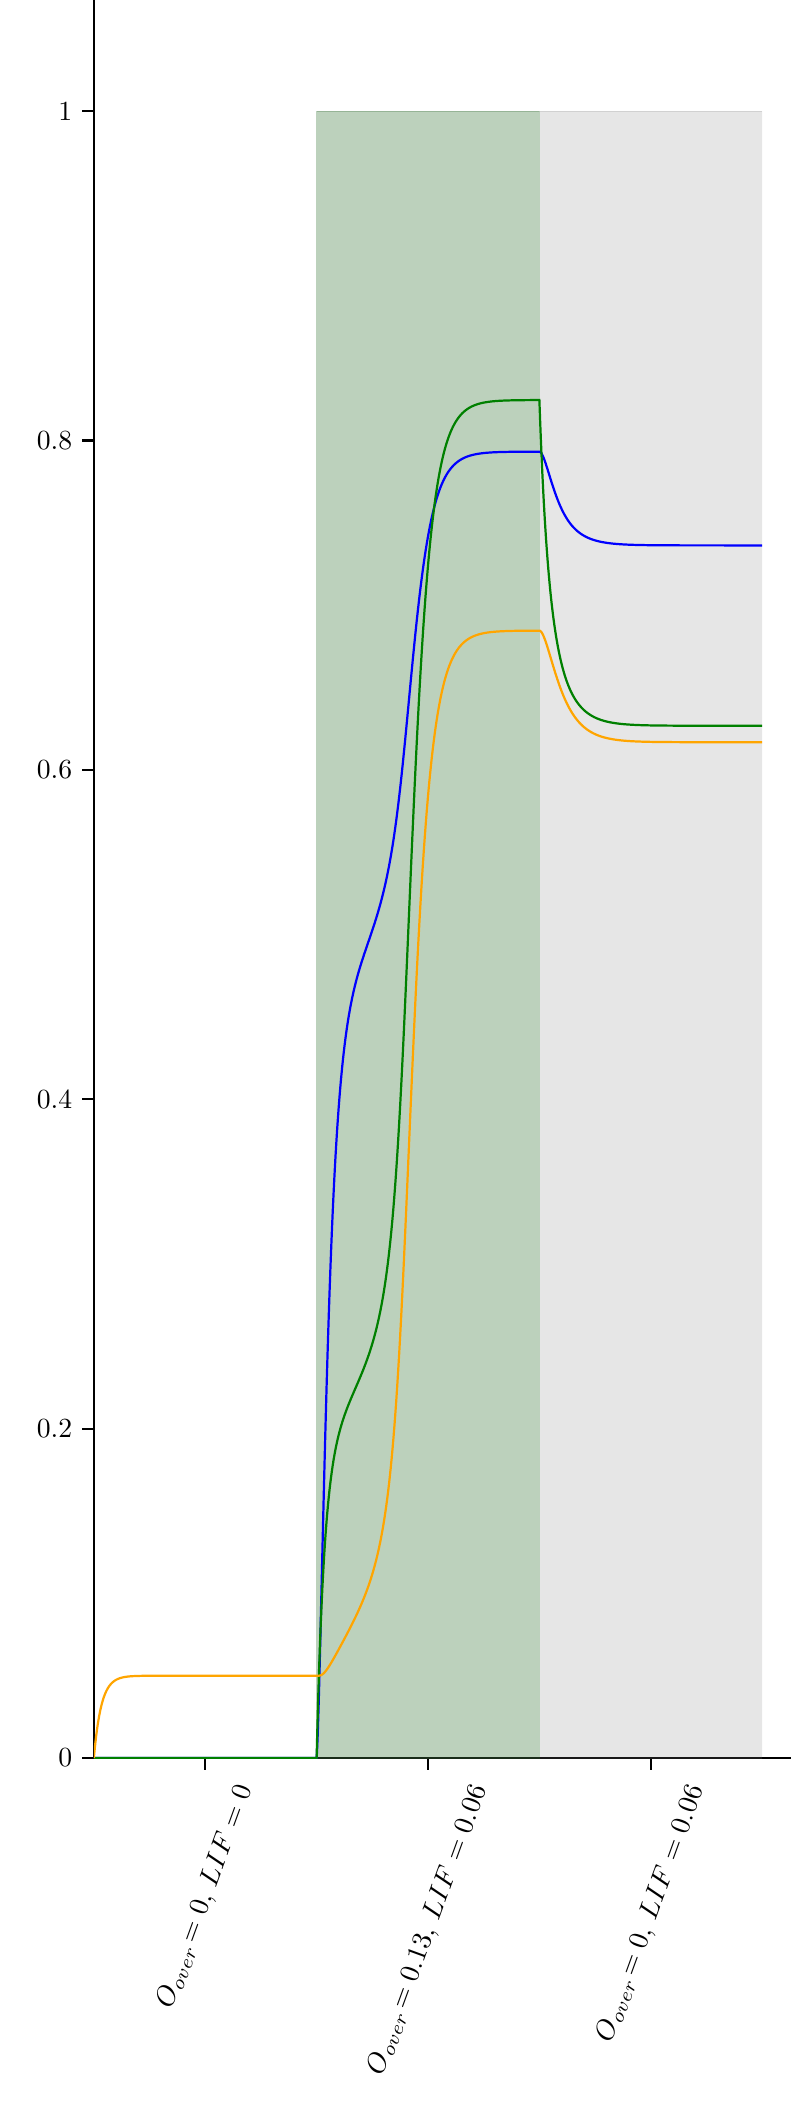
\begin{tikzpicture}[baseline]

\definecolor{darkgray176}{RGB}{176,176,176}
\definecolor{gray}{RGB}{128,128,128}
\definecolor{green}{RGB}{0,128,0}
\definecolor{lightgray204}{RGB}{204,204,204}
\definecolor{orange}{RGB}{255,165,0}

\begin{axis}[
 ytick={0,0.2,0.4,0.6,0.8,1},
 x tick label style = {rotate=70},
 y post scale=3, 
 transpose legend,
legend cell align={left},
legend style={
  fill opacity=0.8,
  draw opacity=1,
  text opacity=1,
  at={(axis cs:5,1.1)},
  anchor=south west,
    legend columns=4,
    /tikz/every even column/.append style={column sep=1.0cm},,
  draw=lightgray204
},
tick align=outside,
tick pos=left,
x grid style={darkgray176},
xmin=0, xmax=90,
xtick style={color=black},
xtick={15,45,75},
xticklabels={
  {\(\displaystyle O_\text{over}\!=0\), \(\displaystyle \text{LIF}=0\)},
  {\(\displaystyle O_\text{over}\!=0.13\), \(\displaystyle \text{LIF}=0.06\)},
  {\(\displaystyle O_\text{over}\!=0\), \(\displaystyle \text{LIF}=0.06\)}
},
y grid style={darkgray176},
ymin=0, ymax=1.05,
ytick style={color=black}
]
\path [draw=green, fill=green, opacity=0.2]
(axis cs:30,0)
--(axis cs:30,1)
--(axis cs:60,1)
--(axis cs:60,0)
--cycle;

\path [draw=gray, fill=gray, opacity=0.2]
(axis cs:30,0)
--(axis cs:30,1)
--(axis cs:90,1)
--(axis cs:90,0)
--cycle;

\addplot [thick, blue]
table {%
0 0
0.0001 0
0.0011 0
0.0111 0
0.1111 0
0.2111 0
0.3111 0
0.4111 0
0.5111 0
0.6111 0
0.7111 0
0.8111 0
0.9111 0
1.0111 0
1.1111 0
1.2111 0
1.3111 0
1.4111 0
1.5111 0
1.6111 0
1.7111 0
1.8111 0
1.9111 0
2.0111 0
2.1111 0
2.2111 0
2.3111 0
2.4111 0
2.5111 0
2.6111 0
2.7111 0
2.8111 0
2.9111 0
3.0111 0
3.1111 0
3.2111 0
3.3111 0
3.4111 0
3.5111 0
3.6111 0
3.7111 0
3.8111 0
3.9111 0
4.0111 0
4.1111 0
4.2111 0
4.3111 0
4.4111 0
4.5111 0
4.6111 0
4.7111 0
4.8111 0
4.9111 0
5.0111 0
5.1111 0
5.2111 0
5.3111 0
5.4111 0
5.5111 0
5.6111 0
5.7111 0
5.8111 0
5.9111 0
6.0111 0
6.1111 0
6.21109999999999 0
6.31109999999999 0
6.41109999999999 0
6.51109999999999 0
6.61109999999999 0
6.71109999999999 0
6.81109999999999 0
6.91109999999999 0
7.01109999999999 0
7.11109999999999 0
7.21109999999999 0
7.31109999999999 0
7.41109999999999 0
7.51109999999999 0
7.61109999999999 0
7.71109999999999 0
7.81109999999999 0
7.91109999999999 0
8.01109999999999 0
8.11109999999999 0
8.21109999999999 0
8.31109999999999 0
8.41109999999999 0
8.51109999999999 0
8.61109999999999 0
8.71109999999999 0
8.81109999999999 0
8.91109999999999 0
9.01109999999998 0
9.11109999999998 0
9.21109999999998 0
9.31109999999998 0
9.41109999999998 0
9.51109999999998 0
9.61109999999998 0
9.71109999999998 0
9.81109999999998 0
9.91109999999998 0
10.0111 0
10.1111 0
10.2111 0
10.3111 0
10.4111 0
10.5111 0
10.6111 0
10.7111 0
10.8111 0
10.9111 0
11.0111 0
11.1111 0
11.2111 0
11.3111 0
11.4111 0
11.5111 0
11.6111 0
11.7111 0
11.8111 0
11.9111 0
12.0111 0
12.1111 0
12.2111 0
12.3111 0
12.4111 0
12.5111 0
12.6111 0
12.7111 0
12.8111 0
12.9111 0
13.0111 0
13.1111 0
13.2111 0
13.3111 0
13.4111 0
13.5111 0
13.6111 0
13.7111 0
13.8111 0
13.9111 0
14.0111 0
14.1111 0
14.2111 0
14.3111 0
14.4111 0
14.5111 0
14.6111 0
14.7111 0
14.8111 0
14.9111 0
15.0111 0
15.1111 0
15.2111 0
15.3111 0
15.4111 0
15.5111 0
15.6111 0
15.7111 0
15.8111 0
15.9111 0
16.0111 0
16.1111 0
16.2111 0
16.3111 0
16.4111 0
16.5111 0
16.6111 0
16.7111 0
16.8111 0
16.9111 0
17.0111 0
17.1111 0
17.2111 0
17.3111 0
17.4111 0
17.5111 0
17.6111 0
17.7111 0
17.8111 0
17.9111 0
18.0111 0
18.1111 0
18.2111 0
18.3111 0
18.4111 0
18.5111 0
18.6111 0
18.7111 0
18.8111 0
18.9111 0
19.0111 0
19.1111 0
19.2111 0
19.3111 0
19.4111 0
19.5111 0
19.6111 0
19.7111 0
19.8111 0
19.9111 0
20.0111 0
20.1111 0
20.2111 0
20.3111 0
20.4111 0
20.5111 0
20.6111 0
20.7111 0
20.8111 0
20.9111 0
21.0111 0
21.1111 0
21.2111 0
21.3111 0
21.4111 0
21.5111 0
21.6111 0
21.7111 0
21.8111 0
21.9111 0
22.0111 0
22.1111 0
22.2111 0
22.3111 0
22.4111000000001 0
22.5111000000001 0
22.6111000000001 0
22.7111000000001 0
22.8111000000001 0
22.9111000000001 0
23.0111000000001 0
23.1111000000001 0
23.2111000000001 0
23.3111000000001 0
23.4111000000001 0
23.5111000000001 0
23.6111000000001 0
23.7111000000001 0
23.8111000000001 0
23.9111000000001 0
24.0111000000001 0
24.1111000000001 0
24.2111000000001 0
24.3111000000001 0
24.4111000000001 0
24.5111000000001 0
24.6111000000001 0
24.7111000000001 0
24.8111000000001 0
24.9111000000001 0
25.0111000000001 0
25.1111000000001 0
25.2111000000001 0
25.3111000000001 0
25.4111000000001 0
25.5111000000001 0
25.6111000000001 0
25.7111000000001 0
25.8111000000001 0
25.9111000000001 0
26.0111000000001 0
26.1111000000001 0
26.2111000000001 0
26.3111000000001 0
26.4111000000001 0
26.5111000000001 0
26.6111000000001 0
26.7111000000001 0
26.8111000000001 0
26.9111000000001 0
27.0111000000001 0
27.1111000000001 0
27.2111000000001 0
27.3111000000001 0
27.4111000000001 0
27.5111000000001 0
27.6111000000001 0
27.7111000000001 0
27.8111000000001 0
27.9111000000001 0
28.0111000000001 0
28.1111000000001 0
28.2111000000001 0
28.3111000000001 0
28.4111000000001 0
28.5111000000001 0
28.6111000000001 0
28.7111000000001 0
28.8111000000001 0
28.9111000000001 0
29.0111000000001 0
29.1111000000001 0
29.2111000000001 0
29.3111000000001 0
29.4111000000002 0
29.5111000000002 0
29.6111000000002 0
29.7111000000002 0
29.8111000000002 0
29.9111000000002 0
30 0
30 0
30.0049204471885 0.000302127534912738
30.0541249190737 0.00403645440599482
30.1541249190737 0.0149693536266964
30.2541249190737 0.0292204052228568
30.3541249190737 0.0457125338809973
30.4541249190737 0.0636456933058862
30.5541249190737 0.0824223248041922
30.6541249190737 0.101594768297675
30.7541249190737 0.120827611690196
30.8541249190737 0.139870425246932
30.9541249190737 0.158537766140675
31.0541249190737 0.17669430556034
31.1541249190737 0.194243604648815
31.2541249190737 0.211119528505097
31.3541249190737 0.227279599803164
31.4541249190737 0.242699802648034
31.5541249190737 0.257370487757574
31.6541249190737 0.271293125571645
31.7541249190737 0.28447771993321
31.8541249190737 0.296940741519047
31.9541249190737 0.308703473612892
32.0541249190737 0.319790687246428
32.1541249190737 0.330229580896585
32.2541249190737 0.340048933632087
32.3541249190737 0.349278431079689
32.4541249190737 0.357948131684232
32.5541249190737 0.366088047068484
32.6541249190737 0.373727815290518
32.7541249190737 0.3808964497627
32.8541249190737 0.38762214976967
32.9541249190737 0.393932161077159
33.0541249190737 0.399852677190733
33.1541249190737 0.405408773504525
33.2541249190737 0.410624367952634
33.3541249190737 0.415522202900752
33.4541249190737 0.420123843940462
33.5541249190737 0.424449692011244
33.6541249190737 0.428519005905385
33.7541249190737 0.432349932732991
33.8541249190737 0.43595954435719
33.9541249190737 0.439363878169278
34.0541249190737 0.442577980872557
34.1541249190737 0.445615954192404
34.2541249190737 0.448491001637145
34.3541249190737 0.451215475606616
34.4541249190737 0.453800924288615
34.5541249190737 0.456258137902596
34.6541249190737 0.458597193948813
34.7541249190737 0.460827501203107
34.8541249190737 0.462957842265256
34.9541249190737 0.464996414524677
35.0541249190737 0.466950869453162
35.1541249190737 0.468828350171863
35.2541249190737 0.470635527270248
35.3541249190737 0.472378632879459
35.4541249190737 0.474063493022223
35.5541249190737 0.475695558277199
35.6541249190737 0.477279932807849
35.7541249190737 0.478821401815407
35.8541249190737 0.480324457482569
35.9541249190737 0.481793323479659
36.0541249190737 0.483231978108609
36.1541249190737 0.484644176162249
36.2541249190737 0.48603346957761
36.3541249190737 0.487403226962192
36.4541249190737 0.488756652071712
36.5541249190737 0.490096801316855
36.6541249190737 0.491426600375022
36.7541249190737 0.492748859981213
36.8541249190737 0.494066290969938
36.9541249190737 0.495381518637513
37.0541249190738 0.496697096491271
37.1541249190738 0.498015519449068
37.2541249190738 0.499339236549019
37.3541249190738 0.500670663225523
37.4541249190738 0.502012193203315
37.5541249190738 0.503366210056384
37.6541249190738 0.504735098473005
37.7541249190738 0.506121255261588
37.8541249190738 0.507527100124518
37.9541249190738 0.508955086218145
38.0541249190738 0.510407710506518
38.1541249190738 0.511887523903792
38.2541249190738 0.513397141185167
38.3541249190738 0.514939250628217
38.4541249190738 0.51651662332498
38.5541249190738 0.518132122079663
38.6541249190738 0.519788709776551
38.7541249190738 0.521489457067111
38.8541249190738 0.523237549183626
38.9541249190738 0.52503629163848
39.0541249190738 0.526889114512937
39.1541249190738 0.528799574976851
39.2541249190738 0.530771357611389
39.3541249190738 0.532808272031561
39.4541249190738 0.534914247225815
39.5541249190738 0.537093321949278
39.6541249190738 0.539349630429888
39.7541249190738 0.541687382579226
39.8541249190738 0.544110837851005
39.9541249190738 0.546624271871296
40.0541249190738 0.549231934989418
40.1541249190738 0.551938001983196
40.2541249190738 0.554746512314338
40.3541249190738 0.557661300586531
40.4541249190738 0.560685917225166
40.5541249190738 0.563823539882493
40.6541249190738 0.567076876674577
40.7541249190738 0.570448063061922
40.8541249190738 0.573938554960937
40.9541249190738 0.577549021465644
41.0541249190738 0.58127924129494
41.1541249190738 0.5851280076724
41.2541249190738 0.589093046698192
41.3541249190738 0.593170954299054
41.4541249190738 0.597357156477572
41.5541249190738 0.601645896800135
41.6541249190738 0.606030253887285
41.7541249190738 0.610502190177654
41.8541249190738 0.615052631551778
41.9541249190738 0.619671575681216
42.0541249190738 0.624348225377458
42.1541249190738 0.629071141904681
42.2541249190738 0.633828412303935
42.3541249190738 0.638607824315701
42.4541249190738 0.64339704248898
42.5541249190738 0.648183779483254
42.6541249190738 0.652955957321774
42.7541249190738 0.657701854335848
42.8541249190738 0.662410234640266
42.9541249190738 0.667070458098418
43.0541249190738 0.671672569789383
43.1541249190738 0.67620736891839
43.2541249190738 0.68066645788076
43.3541249190738 0.685042272782856
43.4541249190738 0.689328097144086
43.5541249190738 0.693518060766047
43.6541249190738 0.697607125880331
43.7541249190738 0.701591062700797
43.8541249190738 0.705466416434878
43.9541249190738 0.709230467675938
44.0541249190738 0.712881187925861
44.1541249190739 0.716417191801523
44.2541249190739 0.719837687274527
44.3541249190739 0.723142425091029
44.4541249190739 0.726331648325209
44.5541249190739 0.729406042840828
44.6541249190739 0.732366689273388
44.7541249190739 0.735215017001962
44.8541249190739 0.737952760455063
44.9541249190739 0.740581917988329
45.0541249190739 0.743104713482232
45.1541249190739 0.745523560733917
45.2541249190739 0.747841030657163
45.3541249190739 0.750059821256487
45.4541249190739 0.752182730304156
45.5541249190739 0.754212630620574
45.6541249190739 0.756152447837981
45.7541249190739 0.758005140513159
45.8541249190739 0.759773682445909
45.9541249190739 0.76146104705535
46.0541249190739 0.763070193664818
46.1541249190739 0.764604055547523
46.2541249190739 0.766065529588572
46.3541249190739 0.767457467423959
46.4541249190739 0.76878266792324
46.5541249190739 0.770043870889502
46.6541249190739 0.771243751857576
46.7541249190739 0.772384917879102
46.8541249190739 0.773469904190734
46.9541249190739 0.774501171669401
47.0541249190739 0.775481104986047
47.1541249190739 0.776412011376426
47.2541249190739 0.777296119954499
47.3541249190739 0.778135581500485
47.4541249190739 0.778932468661839
47.5541249190739 0.779688776511208
47.6541249190739 0.780406423410853
47.7541249190739 0.781087252138013
47.8541249190739 0.781733031230368
47.9541249190739 0.782345456515025
48.0541249190739 0.782926152788387
48.1541249190739 0.783476675617857
48.2541249190739 0.783998513239633
48.3541249190739 0.784493088529824
48.4541249190739 0.784961761028855
48.5541249190739 0.785405829001562
48.6541249190739 0.785826531517634
48.7541249190739 0.78622505053905
48.8541249190739 0.786602513002945
48.9541249190739 0.786959992890015
49.0541249190739 0.78729851326994
49.1541249190739 0.787619048316681
49.2541249190739 0.787922525287606
49.3541249190739 0.788209826461452
49.4541249190739 0.788481791031034
49.5541249190739 0.788739216947429
49.6541249190739 0.78898286271304
49.7541249190739 0.789213449121629
49.8541249190739 0.789431660943885
49.9541249190739 0.789638148557633
50.0541249190739 0.789833529522165
50.1541249190739 0.79001839009655
50.2541249190739 0.790193286702092
50.3541249190739 0.790358747329365
50.4541249190739 0.790515272890467
50.5541249190739 0.790663338517368
50.6541249190739 0.790803394807318
50.7541249190739 0.790935869016479
50.8541249190739 0.791061166203012
50.9541249190739 0.791179670320941
51.0541249190739 0.791291745266189
51.154124919074 0.791397735876228
51.254124919074 0.791497968884818
51.354124919074 0.791592753833329
51.454124919074 0.791682383940156
51.554124919074 0.791767136929735
51.654124919074 0.791847275822668
51.754124919074 0.79192304968844
51.854124919074 0.791994694362202
51.954124919074 0.792062433127063
52.054124919074 0.792126477363312
52.154124919074 0.792187027165956
52.254124919074 0.792244271931919
52.354124919074 0.792298390918226
52.454124919074 0.79234955377244
52.554124919074 0.792397921036603
52.654124919074 0.792443644625857
52.754124919074 0.792486868282928
52.854124919074 0.792527728009565
52.954124919074 0.792566352476024
53.054124919074 0.79260286340963
53.154124919074 0.792637375963407
53.254124919074 0.792669999065734
53.354124919074 0.79270083575194
53.454124919074 0.792729983478726
53.554124919074 0.792757534422242
53.654124919074 0.792783575760637
53.754124919074 0.792808189941837
53.854124919074 0.792831454937304
53.954124919074 0.792853444482464
54.054124919074 0.792874228304488
54.154124919074 0.792893872338049
54.254124919074 0.792912438929687
54.354124919074 0.792929987031339
54.454124919074 0.792946572383617
54.554124919074 0.79296224768933
54.654124919074 0.792977062777778
54.754124919074 0.792991064760282
54.854124919074 0.793004298177414
54.954124919074 0.793016805138344
55.054124919074 0.793028625452734
55.154124919074 0.793039796755559
55.254124919074 0.793050354625218
55.354124919074 0.793060332695314
55.454124919074 0.7930697627604
55.554124919074 0.793078674876045
55.654124919074 0.793087097453497
55.754124919074 0.793095057349238
55.854124919074 0.793102579949702
55.954124919074 0.793109689251415
56.054124919074 0.793116407936793
56.154124919074 0.793122757445845
56.254124919074 0.793128758043977
56.354124919074 0.793134428886134
56.454124919074 0.793139788077447
56.554124919074 0.793144852730597
56.654124919074 0.79314963902006
56.754124919074 0.793154162233396
56.854124919074 0.793158436819758
56.954124919074 0.793162476435754
57.054124919074 0.793166293988816
57.154124919074 0.793169901678201
57.254124919074 0.793173311033764
57.354124919074 0.793176532952608
57.454124919074 0.793179577733747
57.554124919074 0.793182455110862
57.654124919074 0.793185174283285
57.754124919074 0.793187743945276
57.854124919074 0.793190172313712
57.954124919074 0.793192467154255
58.054124919074 0.793194635806095
58.1541249190741 0.793196685205334
58.2541249190741 0.7931986219071
58.3541249190741 0.793200452106442
58.4541249190741 0.793202181658082
58.5541249190741 0.793203816095098
58.6541249190741 0.793205360646563
58.7541249190741 0.793206820254241
58.8541249190741 0.79320819958835
58.9541249190741 0.793209503062471
59.0541249190741 0.793210734847636
59.1541249190741 0.79321189888565
59.2541249190741 0.793212998901673
59.3541249190741 0.793214038416119
59.4541249190741 0.793215020755902
59.5541249190741 0.793215949065064
59.6541249190741 0.793216826314818
59.7541249190741 0.793217655313044
59.8541249190741 0.793218438713262
59.9541249190741 0.79321917902311
60 0.793219504877539
60 0.793219504877539
60.1 0.793073794680546
60.2 0.792664712361178
60.3 0.792032675819707
60.4 0.791213484214853
60.5 0.790238772984429
60.6 0.789136429897268
60.7 0.787930974876685
60.8 0.786643906200868
60.9 0.78529401555514
61 0.783897674283499
61.1 0.782469093061182
61.2 0.781020557086058
61.3 0.779562638764469
61.4 0.778104389747037
61.5 0.776653514052324
61.6 0.775216523901666
61.7 0.77379887977736
61.8 0.772405116109183
61.9 0.771038953891306
62 0.769703401433348
62.1 0.768400844355778
62.2 0.767133125851358
62.3 0.765901618150787
62.4 0.764707286052242
62.5 0.763550743301098
62.6 0.762432302537518
62.7 0.761352019465945
62.8 0.760309731841317
62.9 0.759305093812248
63 0.758337606110912
63.1 0.757406642532982
63.2 0.756511473108363
63.3 0.755651284324399
63.4 0.754825196727523
63.5 0.754032280196755
63.6000000000001 0.75327156715275
63.7000000000001 0.752542063939098
63.8000000000001 0.751842760588091
63.9000000000001 0.751172639160921
64.0000000000001 0.750530680832185
64.1000000000001 0.749915871870382
64.2 0.749327208649683
64.3 0.748763701813464
64.4 0.74822437969679
64.5 0.747708291103047
64.6 0.747214507519192
64.7 0.746742124844445
64.8 0.746290264698611
64.9 0.745858075368503
65 0.745444732444014
65.1 0.74504943918927
65.2 0.744671426688734
65.3 0.744309953803315
65.4 0.743964306967125
65.5 0.743633799851692
65.6 0.743317772921013
65.7 0.743015592897765
65.8 0.742726652158328
65.8999999999999 0.742450368071892
65.9999999999999 0.742186182296811
66.0999999999999 0.741933560045526
66.1999999999999 0.741691989327766
66.2999999999999 0.741460980180268
66.3999999999999 0.741240063890052
66.4999999999999 0.74102879221715
66.5999999999999 0.74082673662174
66.6999999999999 0.740633487499819
66.7999999999999 0.74044865343079
66.8999999999999 0.74027186043971
66.9999999999999 0.740102751276441
67.0999999999999 0.739940984713399
67.1999999999999 0.739786234863258
67.2999999999999 0.739638190517576
67.3999999999999 0.739496554507031
67.4999999999999 0.739361043083683
67.5999999999999 0.739231385325488
67.6999999999998 0.739107322563085
67.7999999999998 0.738988607828742
67.8999999999998 0.738875005327216
67.9999999999998 0.738766289928178
68.0999999999998 0.738662246679774
68.1999999999998 0.738562670342827
68.2999999999998 0.738467364945125
68.3999999999998 0.738376143355215
68.4999999999998 0.73828882687508
68.5999999999998 0.738205244851063
68.6999999999998 0.738125234302397
68.7999999999998 0.738048639566664
68.8999999999998 0.737975311961562
68.9999999999998 0.737905109462295
69.0999999999998 0.737837896393968
69.1999999999998 0.73777354313834
69.2999999999998 0.737711925854329
69.3999999999997 0.737652926211654
69.4999999999997 0.73759643113704
69.5999999999997 0.737542332572405
69.6999999999997 0.737490527244498
69.7999999999997 0.737440916445437
69.8999999999997 0.737393405823658
69.9999999999997 0.737347905184766
70.0999999999997 0.737304328301836
70.1999999999997 0.737262592734697
70.2999999999997 0.737222619657778
70.3999999999997 0.737184333696101
70.4999999999997 0.737147662769023
70.5999999999997 0.737112537941358
70.6999999999997 0.737078893281517
70.7999999999997 0.737046665726314
70.8999999999997 0.737015794952138
70.9999999999997 0.736986223252152
71.0999999999997 0.736957895419243
71.1999999999996 0.736930758634435
71.2999999999996 0.736904762360503
71.3999999999996 0.736879858240527
71.4999999999996 0.736856000001151
71.5999999999996 0.73683314336032
71.6999999999996 0.736811245939271
71.7999999999996 0.736790267178576
71.8999999999996 0.736770168258037
71.9999999999996 0.736750912020257
72.0999999999996 0.736732462897692
72.1999999999996 0.736714786843034
72.2999999999996 0.736697851262762
72.3999999999996 0.736681624953692
72.4999999999996 0.736666078042413
72.5999999999996 0.736651181927441
72.6999999999996 0.736636909223989
72.7999999999996 0.736623233711206
72.8999999999996 0.736610130281786
72.9999999999995 0.736597574893829
73.0999999999995 0.736585544524839
73.1999999999995 0.736574017127782
73.2999999999995 0.736562971589086
73.3999999999995 0.736552387688498
73.4999999999995 0.736542246060725
73.5999999999995 0.736532528158761
73.6999999999995 0.736523216218824
73.7999999999995 0.736514293226842
73.8999999999995 0.736505742886403
73.9999999999995 0.736497549588106
74.0999999999995 0.736489698380256
74.1999999999995 0.736482174940832
74.2999999999995 0.736474965550678
74.3999999999995 0.736468057067858
74.4999999999995 0.73646143690312
74.5999999999995 0.736455092996431
74.6999999999994 0.73644901379452
74.7999999999994 0.73644318822939
74.8999999999994 0.736437605697764
74.9999999999994 0.736432256041406
75.0999999999994 0.736427129528301
75.1999999999994 0.736422216834626
75.2999999999994 0.736417509027515
75.3999999999994 0.736412997548543
75.4999999999994 0.736408674197929
75.5999999999994 0.736404531119414
75.6999999999994 0.736400560785775
75.7999999999994 0.736396755984967
75.8999999999994 0.736393109806852
75.9999999999994 0.736389615630493
76.0999999999994 0.736386267111984
76.1999999999994 0.736383058172808
76.2999999999994 0.736379982988679
76.3999999999994 0.736377035978861
76.4999999999993 0.736374211795939
76.5999999999993 0.736371505316026
76.6999999999993 0.736368911629382
76.7999999999993 0.73636642603143
76.8999999999993 0.736364044014152
76.9999999999993 0.736361761257848
77.0999999999993 0.736359573623243
77.1999999999993 0.73635747714393
77.2999999999993 0.736355468019125
77.3999999999993 0.736353542606735
77.4999999999993 0.73635169741671
77.5999999999993 0.736349929104685
77.6999999999993 0.736348234465876
77.7999999999993 0.736346610429248
77.8999999999993 0.736345054051915
77.9999999999993 0.736343562513784
78.0999999999993 0.736342133112418
78.1999999999992 0.736340763258121
78.2999999999992 0.736339450469223
78.3999999999992 0.736338192367567
78.4999999999992 0.736336986674182
78.5999999999992 0.736335831205143
78.6999999999992 0.736334723867597
78.7999999999992 0.736333662655962
78.8999999999992 0.736332645648283
78.9999999999992 0.736331671002736
79.0999999999992 0.736330736954289
79.1999999999992 0.736329841811491
79.2999999999992 0.736328983953403
79.3999999999992 0.736328161826657
79.4999999999992 0.736327373942632
79.5999999999992 0.736326618874758
79.6999999999992 0.73632589525592
79.7999999999992 0.736325201775984
79.8999999999992 0.736324537179417
79.9999999999991 0.73632390026301
80.0999999999991 0.736323289873694
80.1999999999991 0.736322704906454
80.2999999999991 0.736322144302317
80.3999999999991 0.736321607046441
80.4999999999991 0.736321092166267
80.5999999999991 0.736320598729761
80.6999999999991 0.736320125843723
80.7999999999991 0.736319672652167
80.8999999999991 0.73631923833477
80.9999999999991 0.736318822105389
81.0999999999991 0.736318423210628
81.1999999999991 0.736318040928483
81.2999999999991 0.736317674567025
81.3999999999991 0.736317323463153
81.4999999999991 0.736316986981388
81.5999999999991 0.736316664512724
81.6999999999991 0.736316355473525
81.799999999999 0.736316059304466
81.899999999999 0.736315775469522
81.999999999999 0.736315503454996
82.099999999999 0.736315242768588
82.199999999999 0.736314992938507
82.299999999999 0.736314753512609
82.399999999999 0.736314524057589
82.499999999999 0.736314304158185
82.599999999999 0.736314093416434
82.699999999999 0.736313891450949
82.799999999999 0.736313697896228
82.899999999999 0.736313512401991
82.999999999999 0.73631333463255
83.099999999999 0.736313164266196
83.199999999999 0.73631300099462
83.299999999999 0.736312844522355
83.399999999999 0.736312694566238
83.4999999999989 0.736312550854901
83.5999999999989 0.736312413128277
83.6999999999989 0.73631228113713
83.7999999999989 0.736312154642607
83.8999999999989 0.736312033415798
83.9999999999989 0.736311917237331
84.0999999999989 0.736311805896969
84.1999999999989 0.736311699193228
84.2999999999989 0.73631159693302
84.3999999999989 0.736311498931293
84.4999999999989 0.736311405010707
84.5999999999989 0.736311315001305
84.6999999999989 0.736311228740207
84.7999999999989 0.736311146071319
84.8999999999989 0.736311066845046
84.9999999999989 0.736310990918022
85.0999999999989 0.736310918152854
85.1999999999989 0.73631084841787
85.2999999999988 0.73631078158688
85.3999999999988 0.736310717538951
85.4999999999988 0.736310656158186
85.5999999999988 0.736310597333514
85.6999999999988 0.736310540958489
85.7999999999988 0.7363104869311
85.8999999999988 0.736310435153581
85.9999999999988 0.736310385532241
86.0999999999988 0.736310337977289
86.1999999999988 0.736310292402672
86.2999999999988 0.736310248725922
86.3999999999988 0.736310206868007
86.4999999999988 0.736310166753182
86.5999999999988 0.736310128308861
86.6999999999988 0.736310091465478
86.7999999999988 0.736310056156364
86.8999999999988 0.736310022317627
86.9999999999987 0.736309989888036
87.0999999999987 0.73630995880891
87.1999999999987 0.736309929024011
87.2999999999987 0.736309900479443
87.3999999999987 0.736309873123554
87.4999999999987 0.736309846906845
87.5999999999987 0.736309821781876
87.6999999999987 0.736309797703184
87.7999999999987 0.736309774627199
87.8999999999987 0.736309752512164
87.9999999999987 0.736309731318064
88.0999999999987 0.736309711006547
88.1999999999987 0.736309691540859
88.2999999999987 0.736309672885779
88.3999999999987 0.73630965500755
88.4999999999987 0.736309637873821
88.5999999999987 0.736309621453589
88.6999999999987 0.736309605717142
88.7999999999986 0.736309590636006
88.8999999999986 0.736309576182891
88.9999999999986 0.736309562331644
89.0999999999986 0.736309549057203
89.1999999999986 0.736309536335547
89.2999999999986 0.736309524143656
89.3999999999986 0.736309512459469
89.4999999999986 0.736309501261845
89.5999999999986 0.736309490530522
89.6999999999986 0.736309480246081
89.7999999999986 0.736309470389912
89.8999999999986 0.736309460944182
89.9999999999986 0.736309451891799
90 0.736309451891799
};
\addplot [thick, green]
table {%
0 0
0.0001 0
0.0011 0
0.0111 0
0.1111 0
0.2111 0
0.3111 0
0.4111 0
0.5111 0
0.6111 0
0.7111 0
0.8111 0
0.9111 0
1.0111 0
1.1111 0
1.2111 0
1.3111 0
1.4111 0
1.5111 0
1.6111 0
1.7111 0
1.8111 0
1.9111 0
2.0111 0
2.1111 0
2.2111 0
2.3111 0
2.4111 0
2.5111 0
2.6111 0
2.7111 0
2.8111 0
2.9111 0
3.0111 0
3.1111 0
3.2111 0
3.3111 0
3.4111 0
3.5111 0
3.6111 0
3.7111 0
3.8111 0
3.9111 0
4.0111 0
4.1111 0
4.2111 0
4.3111 0
4.4111 0
4.5111 0
4.6111 0
4.7111 0
4.8111 0
4.9111 0
5.0111 0
5.1111 0
5.2111 0
5.3111 0
5.4111 0
5.5111 0
5.6111 0
5.7111 0
5.8111 0
5.9111 0
6.0111 0
6.1111 0
6.21109999999999 0
6.31109999999999 0
6.41109999999999 0
6.51109999999999 0
6.61109999999999 0
6.71109999999999 0
6.81109999999999 0
6.91109999999999 0
7.01109999999999 0
7.11109999999999 0
7.21109999999999 0
7.31109999999999 0
7.41109999999999 0
7.51109999999999 0
7.61109999999999 0
7.71109999999999 0
7.81109999999999 0
7.91109999999999 0
8.01109999999999 0
8.11109999999999 0
8.21109999999999 0
8.31109999999999 0
8.41109999999999 0
8.51109999999999 0
8.61109999999999 0
8.71109999999999 0
8.81109999999999 0
8.91109999999999 0
9.01109999999998 0
9.11109999999998 0
9.21109999999998 0
9.31109999999998 0
9.41109999999998 0
9.51109999999998 0
9.61109999999998 0
9.71109999999998 0
9.81109999999998 0
9.91109999999998 0
10.0111 0
10.1111 0
10.2111 0
10.3111 0
10.4111 0
10.5111 0
10.6111 0
10.7111 0
10.8111 0
10.9111 0
11.0111 0
11.1111 0
11.2111 0
11.3111 0
11.4111 0
11.5111 0
11.6111 0
11.7111 0
11.8111 0
11.9111 0
12.0111 0
12.1111 0
12.2111 0
12.3111 0
12.4111 0
12.5111 0
12.6111 0
12.7111 0
12.8111 0
12.9111 0
13.0111 0
13.1111 0
13.2111 0
13.3111 0
13.4111 0
13.5111 0
13.6111 0
13.7111 0
13.8111 0
13.9111 0
14.0111 0
14.1111 0
14.2111 0
14.3111 0
14.4111 0
14.5111 0
14.6111 0
14.7111 0
14.8111 0
14.9111 0
15.0111 0
15.1111 0
15.2111 0
15.3111 0
15.4111 0
15.5111 0
15.6111 0
15.7111 0
15.8111 0
15.9111 0
16.0111 0
16.1111 0
16.2111 0
16.3111 0
16.4111 0
16.5111 0
16.6111 0
16.7111 0
16.8111 0
16.9111 0
17.0111 0
17.1111 0
17.2111 0
17.3111 0
17.4111 0
17.5111 0
17.6111 0
17.7111 0
17.8111 0
17.9111 0
18.0111 0
18.1111 0
18.2111 0
18.3111 0
18.4111 0
18.5111 0
18.6111 0
18.7111 0
18.8111 0
18.9111 0
19.0111 0
19.1111 0
19.2111 0
19.3111 0
19.4111 0
19.5111 0
19.6111 0
19.7111 0
19.8111 0
19.9111 0
20.0111 0
20.1111 0
20.2111 0
20.3111 0
20.4111 0
20.5111 0
20.6111 0
20.7111 0
20.8111 0
20.9111 0
21.0111 0
21.1111 0
21.2111 0
21.3111 0
21.4111 0
21.5111 0
21.6111 0
21.7111 0
21.8111 0
21.9111 0
22.0111 0
22.1111 0
22.2111 0
22.3111 0
22.4111000000001 0
22.5111000000001 0
22.6111000000001 0
22.7111000000001 0
22.8111000000001 0
22.9111000000001 0
23.0111000000001 0
23.1111000000001 0
23.2111000000001 0
23.3111000000001 0
23.4111000000001 0
23.5111000000001 0
23.6111000000001 0
23.7111000000001 0
23.8111000000001 0
23.9111000000001 0
24.0111000000001 0
24.1111000000001 0
24.2111000000001 0
24.3111000000001 0
24.4111000000001 0
24.5111000000001 0
24.6111000000001 0
24.7111000000001 0
24.8111000000001 0
24.9111000000001 0
25.0111000000001 0
25.1111000000001 0
25.2111000000001 0
25.3111000000001 0
25.4111000000001 0
25.5111000000001 0
25.6111000000001 0
25.7111000000001 0
25.8111000000001 0
25.9111000000001 0
26.0111000000001 0
26.1111000000001 0
26.2111000000001 0
26.3111000000001 0
26.4111000000001 0
26.5111000000001 0
26.6111000000001 0
26.7111000000001 0
26.8111000000001 0
26.9111000000001 0
27.0111000000001 0
27.1111000000001 0
27.2111000000001 0
27.3111000000001 0
27.4111000000001 0
27.5111000000001 0
27.6111000000001 0
27.7111000000001 0
27.8111000000001 0
27.9111000000001 0
28.0111000000001 0
28.1111000000001 0
28.2111000000001 0
28.3111000000001 0
28.4111000000001 0
28.5111000000001 0
28.6111000000001 0
28.7111000000001 0
28.8111000000001 0
28.9111000000001 0
29.0111000000001 0
29.1111000000001 0
29.2111000000001 0
29.3111000000001 0
29.4111000000002 0
29.5111000000002 0
29.6111000000002 0
29.7111000000002 0
29.8111000000002 0
29.9111000000002 0
30 0
30 0
30.0049204471885 0.000932588708472422
30.0541249190737 0.0100104031483612
30.1541249190737 0.0271402277604621
30.2541249190737 0.0426500552157587
30.3541249190737 0.0567110128723739
30.4541249190737 0.06948133855795
30.5541249190737 0.0811022576095053
30.6541249190737 0.0916969169388807
30.7541249190737 0.101371854439609
30.8541249190737 0.110219520971803
30.9541249190737 0.118320813698285
31.0541249190737 0.125747190428548
31.1541249190737 0.132562300190494
31.2541249190737 0.138823208163105
31.3541249190737 0.144581320100485
31.4541249190737 0.149883095736759
31.5541249190737 0.154770616452695
31.6541249190737 0.159282051576152
31.7541249190737 0.163452052494466
31.8541249190737 0.167312093547222
31.9541249190737 0.17089077207673
32.0541249190737 0.174214075844732
32.1541249190737 0.177305623409968
32.2541249190737 0.180186881422752
32.3541249190737 0.182877361758514
32.4541249190737 0.185394800749939
32.5541249190737 0.187755322343336
32.6541249190737 0.189973586711175
32.7541249190737 0.192062925645574
32.8541249190737 0.194035465904148
32.9541249190737 0.195902241560261
33.0541249190737 0.197673296312166
33.1541249190737 0.199357776622621
33.2541249190737 0.200964016487756
33.3541249190737 0.202499614568739
33.4541249190737 0.203971504360329
33.5541249190737 0.205386018015862
33.6541249190737 0.206748944397868
33.7541249190737 0.20806558187694
33.8541249190737 0.209340786358386
33.9541249190737 0.210579014976379
34.0541249190737 0.211784365858502
34.1541249190737 0.212960614329688
34.2541249190737 0.214111245893331
34.3541249190737 0.215239486298664
34.4541249190737 0.216348328977235
34.5541249190737 0.217440560107279
34.6541249190737 0.218518781542813
34.7541249190737 0.219585431824334
34.8541249190737 0.220642805469833
34.9541249190737 0.221693070728355
35.0541249190737 0.222738285963515
35.1541249190737 0.223780414820918
35.2541249190737 0.22482134032145
35.3541249190737 0.225862878011596
35.4541249190737 0.226906788292405
35.5541249190737 0.227954788040206
35.6541249190737 0.229008561624769
35.7541249190737 0.230069771424066
35.8541249190737 0.23114006792925
35.9541249190737 0.232221099528666
36.0541249190737 0.233314522055768
36.1541249190737 0.234422008182578
36.2541249190737 0.235545256737789
36.3541249190737 0.236686002026686
36.4541249190737 0.237846023228797
36.5541249190737 0.239027153948406
36.6541249190737 0.240231291992784
36.7541249190737 0.241460409453181
36.8541249190737 0.242716563164134
36.9541249190737 0.244001905617409
37.0541249190738 0.245318696407839
37.1541249190738 0.246669314289282
37.2541249190738 0.248056269919635
37.3541249190738 0.249482219374275
37.4541249190738 0.250949978506929
37.5541249190738 0.252462538235616
37.6541249190738 0.254023080828415
37.7541249190738 0.255634997258783
37.8541249190738 0.257301905692332
37.9541249190738 0.259027671155375
38.0541249190738 0.260816426419104
38.1541249190738 0.262672594110562
38.2541249190738 0.264600910030943
38.3541249190738 0.266606447621209
38.4541249190738 0.268694643462103
38.5541249190738 0.270871323627589
38.6541249190738 0.273142730624329
38.7541249190738 0.275515550541311
38.8541249190738 0.27799693989927
38.9541249190738 0.280594551524824
39.0541249190738 0.283316558575296
39.1541249190738 0.286171675603238
39.2541249190738 0.289169175272363
39.3541249190738 0.292318899018317
39.4541249190738 0.295631259591181
39.5541249190738 0.299117233029286
39.6541249190738 0.302788337209974
39.7541249190738 0.306656593725412
39.8541249190738 0.310734469474895
39.9541249190738 0.315034794096915
40.0541249190738 0.319570649247329
40.1541249190738 0.32435522584126
40.2541249190738 0.329401645804897
40.3541249190738 0.334722745723137
40.4541249190738 0.340330821107878
40.5541249190738 0.346237331914174
40.6541249190738 0.352452572416975
40.7541249190738 0.35898531157955
40.8541249190738 0.365842413453052
40.9541249190738 0.373028450694739
41.0541249190738 0.380545327622975
41.1541249190738 0.388391931901316
41.2541249190738 0.396563835491221
41.3541249190738 0.405053065507053
41.4541249190738 0.413847963754383
41.5541249190738 0.42293314995433
41.6541249190738 0.432289598142422
41.7541249190738 0.441894828943629
41.8541249190738 0.451723213050022
41.9541249190738 0.461746374065604
42.0541249190738 0.471933672719716
42.1541249190738 0.482252749924343
42.2541249190738 0.492670103654158
42.3541249190738 0.503151674263003
42.4541249190738 0.513663414441971
42.5541249190738 0.524171823183073
42.6541249190738 0.534644427324913
42.7541249190738 0.54505019897908
42.8541249190738 0.555359901873177
42.9541249190738 0.565546364005772
43.0541249190738 0.5755846777236
43.1541249190738 0.585452331260984
43.2541249190738 0.595129277892537
43.3541249190738 0.604597950190211
43.4541249190738 0.613843227544516
43.5541249190738 0.622852365233362
43.6541249190738 0.631614893032759
43.7541249190738 0.640122490786065
43.8541249190738 0.648368847590628
43.9541249190738 0.656349510410771
44.0541249190738 0.66406172705184
44.1541249190739 0.671504287580137
44.2541249190739 0.678677367480816
44.3541249190739 0.685582375129628
44.4541249190739 0.692221805524432
44.5541249190739 0.698599101680795
44.6541249190739 0.704718524640081
44.7541249190739 0.710585032662172
44.8541249190739 0.716204169870577
44.9541249190739 0.721581964376681
45.0541249190739 0.72672483572343
45.1541249190739 0.731639511348686
45.2541249190739 0.73633295166699
45.3541249190739 0.740812283298748
45.4541249190739 0.745084739931764
45.5541249190739 0.749157610276432
45.6541249190739 0.753038192568252
45.7541249190739 0.756733755075976
45.8541249190739 0.760251502087515
45.9541249190739 0.763598544866269
46.0541249190739 0.766781877095628
46.1541249190739 0.769808354357581
46.2541249190739 0.77268467722119
46.3541249190739 0.775417377547273
46.4541249190739 0.778012807646192
46.5541249190739 0.780477131955536
46.6541249190739 0.782816320933416
46.7541249190739 0.785036146890658
46.8541249190739 0.78714218151124
46.9541249190739 0.789139794834794
47.0541249190739 0.791034155497753
47.1541249190739 0.79283023205079
47.2541249190739 0.794532795189673
47.3541249190739 0.796146420754414
47.4541249190739 0.797675493367897
47.5541249190739 0.799124210599984
47.6541249190739 0.800496587556499
47.7541249190739 0.801796461804671
47.8541249190739 0.803027498557542
47.9541249190739 0.804193196049724
48.0541249190739 0.805296891045695
48.1541249190739 0.806341764429755
48.2541249190739 0.807330846833808
48.3541249190739 0.808267024265414
48.4541249190739 0.809153043704163
48.5541249190739 0.809991518639345
48.6541249190739 0.810784934526276
48.7541249190739 0.811535654142508
48.8541249190739 0.81224592282853
48.9541249190739 0.812917873600562
49.0541249190739 0.813553532125629
49.1541249190739 0.814154821551401
49.2541249190739 0.814723567185226
49.3541249190739 0.815261501018528
49.4541249190739 0.815770266094184
49.5541249190739 0.816251420715782
49.6541249190739 0.816706442498732
49.7541249190739 0.817136732264114
49.8541249190739 0.817543617776924
49.9541249190739 0.817928357331036
50.0541249190739 0.818292143183703
50.1541249190739 0.818636104842877
50.2541249190739 0.818961312210981
50.3541249190739 0.819268778589011
50.4541249190739 0.819559463545107
50.5541249190739 0.819834275651828
50.6541249190739 0.820094075096519
50.7541249190739 0.820339676169199
50.8541249190739 0.820571849632426
50.9541249190739 0.820791324977617
51.0541249190739 0.820998792572225
51.154124919074 0.821194905702193
51.254124919074 0.821380282513969
51.354124919074 0.821555507860338
51.454124919074 0.821721135054196
51.554124919074 0.821877687534316
51.654124919074 0.822025660447015
51.754124919074 0.822165522147543
51.854124919074 0.822297715624878
51.954124919074 0.822422659853481
52.054124919074 0.822540751075459
52.154124919074 0.822652364016439
52.254124919074 0.822757853038348
52.354124919074 0.822857553232137
52.454124919074 0.822951781453417
52.554124919074 0.823040837303785
52.654124919074 0.823125004060568
52.754124919074 0.823204549557536
52.854124919074 0.82327972701907
52.954124919074 0.823350775850122
53.054124919074 0.823417922384231
53.154124919074 0.823481380591718
53.254124919074 0.823541352750127
53.354124919074 0.823598030078839
53.454124919074 0.823651593339729
53.554124919074 0.823702213405614
53.654124919074 0.823750051798189
53.754124919074 0.823795261197037
53.854124919074 0.82383798592123
53.954124919074 0.82387836238497
54.054124919074 0.823916519528634
54.154124919074 0.823952579226531
54.254124919074 0.823986656672597
54.354124919074 0.824018860745209
54.454124919074 0.824049294352225
54.554124919074 0.824078054757307
54.654124919074 0.824105233888526
54.754124919074 0.824130918630204
54.854124919074 0.824155191098882
54.954124919074 0.824178128904274
55.054124919074 0.824199805396014
55.154124919074 0.824220289896959
55.254124919074 0.824239647923777
55.354124919074 0.824257941395498
55.454124919074 0.824275228830689
55.554124919074 0.824291565533868
55.654124919074 0.824307003771722
55.754124919074 0.824321592939718
55.854124919074 0.824335379719583
55.954124919074 0.824348408228188
56.054124919074 0.824360720158282
56.154124919074 0.824372354911525
56.254124919074 0.824383349724237
56.354124919074 0.824393739786265
56.454124919074 0.824403558353335
56.554124919074 0.824412836853256
56.654124919074 0.824421604986294
56.754124919074 0.824429890820055
56.854124919074 0.824437720879155
56.954124919074 0.824445120229983
57.054124919074 0.824452112560812
57.154124919074 0.824458720257507
57.254124919074 0.824464964475097
57.354124919074 0.824470865205398
57.454124919074 0.824476441340947
57.554124919074 0.824481710735404
57.654124919074 0.824486690260658
57.754124919074 0.824491395860787
57.854124919074 0.824495842603054
57.954124919074 0.824500044726109
58.054124919074 0.824504015685538
58.1541249190741 0.824507768196913
58.2541249190741 0.824511314276476
58.3541249190741 0.824514665279588
58.4541249190741 0.824517831937066
58.5541249190741 0.824520824389521
58.6541249190741 0.824523652219815
58.7541249190741 0.824526324483726
58.8541249190741 0.824528849738935
58.9541249190741 0.824531236072413
59.0541249190741 0.824533491126313
59.1541249190741 0.824535622122425
59.2541249190741 0.824537635885298
59.3541249190741 0.824539538864088
59.4541249190741 0.824541337153199
59.5541249190741 0.824543036511796
59.6541249190741 0.824544642382247
59.7541249190741 0.824546159907539
59.8541249190741 0.824547593947752
59.9541249190741 0.824548949095614
60 0.8245495455725
60 0.8245495455725
60.1 0.812051738667754
60.2 0.800496466457774
60.3 0.789801396397768
60.4 0.779892227079572
60.5 0.770701830184923
60.6 0.762169492423098
60.7 0.754240244769192
60.8 0.746864268058895
60.9 0.739996365479035
61 0.733595493761236
61.1 0.727624345972249
61.2 0.722048979726736
61.3 0.716838485449585
61.4 0.711964690004765
61.5 0.707401891602489
61.6 0.703126622410108
61.7 0.699117435736156
61.8 0.695354715041527
61.9 0.691820502365142
62 0.688498344041017
62.1 0.685373151835493
62.2 0.682431077852708
62.3 0.679659401747837
62.4 0.677046428954834
62.5 0.674581398781873
62.6 0.672254401356017
62.7 0.670056302511436
62.8 0.667978675814665
62.9 0.66601374100782
63 0.664154308227855
63.1 0.662393727428134
63.2 0.66072584248903
63.3 0.659144949557811
63.4 0.657645759205643
63.5 0.656223362031867
63.6000000000001 0.654873197383393
63.7000000000001 0.653591024890626
63.8000000000001 0.652372898551385
63.9000000000001 0.651215143121041
64.0000000000001 0.650114332591136
64.1000000000001 0.649067270560202
64.2 0.648070972319791
64.3 0.647122648495987
64.4 0.64621969010222
64.5 0.645359654873148
64.6 0.644540254761902
64.7 0.643759344494319
64.8 0.643014911083913
64.9 0.642305064220532
65 0.641628027453893
65.1 0.640982130100623
65.2 0.640365799810194
65.3 0.639777555731146
65.4 0.639216002224545
65.5 0.638679823076497
65.6 0.638167776166078
65.7 0.637678688549035
65.8 0.637211451921286
65.8999999999999 0.636765018429567
65.9999999999999 0.636338396799546
66.0999999999999 0.635930648754442
66.1999999999999 0.635540885699633
66.2999999999999 0.635168265650971
66.3999999999999 0.634811990386511
66.4999999999999 0.634471302803204
66.5999999999999 0.634145484461745
66.6999999999999 0.633833853304257
66.7999999999999 0.633535761530873
66.8999999999999 0.63325059362248
66.9999999999999 0.632977764498024
67.0999999999999 0.63271671779579
67.1999999999999 0.632466924268975
67.2999999999999 0.632227880286733
67.3999999999999 0.631999106432597
67.4999999999999 0.631780146192912
67.5999999999999 0.631570564728498
67.6999999999998 0.631369947723375
67.7999999999998 0.631177900304857
67.8999999999998 0.630994046029837
67.9999999999998 0.630818025932471
68.0999999999998 0.630649497628906
68.1999999999998 0.630488134475008
68.2999999999998 0.630333624773411
68.3999999999998 0.630185671026468
68.4999999999998 0.63004398923199
68.5999999999998 0.629908308218874
68.6999999999998 0.629778369019973
68.7999999999998 0.629653924279743
68.8999999999998 0.629534737694412
68.9999999999998 0.629420583482566
69.0999999999998 0.629311245884229
69.1999999999998 0.629206518686635
69.2999999999998 0.629106204775036
69.3999999999997 0.629010115707005
69.4999999999997 0.628918071308811
69.5999999999997 0.628829899292536
69.6999999999997 0.628745434892701
69.7999999999997 0.628664520521261
69.8999999999997 0.628587005439894
69.9999999999997 0.6285127454486
70.0999999999997 0.628441602589669
70.1999999999997 0.628373444866172
70.2999999999997 0.628308145974149
70.3999999999997 0.628245585047754
70.4999999999997 0.628185646416638
70.5999999999997 0.628128219374917
70.6999999999997 0.62807319796111
70.7999999999997 0.628020480748445
70.8999999999997 0.627969970645019
70.9999999999997 0.627921574703274
71.0999999999997 0.627875203938319
71.1999999999996 0.627830773154651
71.2999999999996 0.627788200780831
71.3999999999996 0.627747408711743
71.4999999999996 0.627708322158022
71.5999999999996 0.627670869502335
71.6999999999996 0.627634982162141
71.7999999999996 0.62760059445864
71.8999999999996 0.627567643491598
71.9999999999996 0.627536069019768
72.0999999999996 0.627505813346641
72.1999999999996 0.627476821211269
72.2999999999996 0.627449039683924
72.3999999999996 0.62742241806636
72.4999999999996 0.627396907796474
72.5999999999996 0.627372462357145
72.6999999999996 0.627349037189072
72.7999999999996 0.627326589607418
72.8999999999996 0.627305078722087
72.9999999999995 0.627284465361475
73.0999999999995 0.62726471199952
73.1999999999995 0.627245782685928
73.2999999999995 0.627227642979398
73.3999999999995 0.627210259883744
73.4999999999995 0.627193601786765
73.5999999999995 0.627177638401741
73.6999999999995 0.627162340711446
73.7999999999995 0.627147680914564
73.8999999999995 0.627133632374392
73.9999999999995 0.627120169569748
74.0999999999995 0.627107268047966
74.1999999999995 0.627094904379905
74.2999999999995 0.627083056116868
74.3999999999995 0.627071701749359
74.4999999999995 0.627060820667595
74.5999999999995 0.627050393123691
74.6999999999994 0.627040400195455
74.7999999999994 0.627030823751712
74.8999999999994 0.627021646419108
74.9999999999994 0.627012851550303
75.0999999999994 0.627004423193528
75.1999999999994 0.62699634606341
75.2999999999994 0.626988605513048
75.3999999999994 0.626981187507251
75.4999999999994 0.626974078596917
75.5999999999994 0.626967265894485
75.6999999999994 0.626960737050425
75.7999999999994 0.626954480230716
75.8999999999994 0.626948484095273
75.9999999999994 0.62694273777728
76.0999999999994 0.626937230863396
76.1999999999994 0.626931953374788
76.2999999999994 0.626926895748963
76.3999999999994 0.626922048822361
76.4999999999993 0.626917403813686
76.5999999999993 0.626912952307925
76.6999999999993 0.626908686241047
76.7999999999993 0.626904597885337
76.8999999999993 0.626900679835351
76.9999999999993 0.626896924994454
77.0999999999993 0.626893326561925
77.1999999999993 0.626889878020599
77.2999999999993 0.626886573125033
77.3999999999993 0.62688340589016
77.4999999999993 0.626880370580421
77.5999999999993 0.626877461699354
77.6999999999993 0.626874673979612
77.7999999999993 0.626872002373408
77.8999999999993 0.626869442043349
77.9999999999993 0.626866988353663
78.0999999999993 0.626864636861782
78.1999999999992 0.626862383310292
78.2999999999992 0.626860223619199
78.3999999999992 0.626858153878541
78.4999999999992 0.626856170341287
78.5999999999992 0.626854269416549
78.6999999999992 0.626852447663068
78.7999999999992 0.626850701782976
78.8999999999992 0.626849028615817
78.9999999999992 0.626847425132819
79.0999999999992 0.626845888431403
79.1999999999992 0.626844415729924
79.2999999999992 0.626843004362628
79.3999999999992 0.626841651774822
79.4999999999992 0.626840355518244
79.5999999999992 0.62683911324663
79.6999999999992 0.626837922711459
79.7999999999992 0.626836781757881
79.8999999999992 0.626835688320814
79.9999999999991 0.626834640421203
80.0999999999991 0.626833636162432
80.1999999999991 0.626832673726893
80.2999999999991 0.626831751372691
80.3999999999991 0.626830867430491
80.4999999999991 0.626830020300493
80.5999999999991 0.626829208449533
80.6999999999991 0.626828430408313
80.7999999999991 0.626827684768732
80.8999999999991 0.626826970181343
80.9999999999991 0.626826285352906
81.0999999999991 0.626825629044044
81.1999999999991 0.626825000067006
81.2999999999991 0.62682439728351
81.3999999999991 0.626823819602685
81.4999999999991 0.626823265979093
81.5999999999991 0.626822735410842
81.6999999999991 0.626822226937765
81.799999999999 0.626821739639689
81.899999999999 0.626821272634763
81.999999999999 0.626820825077864
82.099999999999 0.626820396159069
82.199999999999 0.626819985102186
82.299999999999 0.626819591163349
82.399999999999 0.626819213629673
82.499999999999 0.626818851817964
82.599999999999 0.62681850507348
82.699999999999 0.626818172768748
82.799999999999 0.626817854302428
82.899999999999 0.626817549098221
82.999999999999 0.626817256603833
83.099999999999 0.626816976289969
83.199999999999 0.626816707649376
83.299999999999 0.626816450195929
83.399999999999 0.626816203463745
83.4999999999989 0.626815967006347
83.5999999999989 0.626815740395848
83.6999999999989 0.626815523222182
83.7999999999989 0.626815315092363
83.8999999999989 0.626815115629767
83.9999999999989 0.626814924473457
84.0999999999989 0.626814741277527
84.1999999999989 0.626814565710476
84.2999999999989 0.626814397454607
84.3999999999989 0.626814236205457
84.4999999999989 0.626814081671238
84.5999999999989 0.626813933572317
84.6999999999989 0.626813791640704
84.7999999999989 0.626813655619571
84.8999999999989 0.626813525262783
84.9999999999989 0.626813400334459
85.0999999999989 0.626813280608536
85.1999999999989 0.62681316586837
85.2999999999988 0.626813055906336
85.3999999999988 0.626812950523457
85.4999999999988 0.626812849529041
85.5999999999988 0.626812752740338
85.6999999999988 0.626812659982208
85.7999999999988 0.626812571086805
85.8999999999988 0.626812485893272
85.9999999999988 0.626812404247451
86.0999999999988 0.626812326001604
86.1999999999988 0.626812251014146
86.2999999999988 0.626812179149386
86.3999999999988 0.626812110277286
86.4999999999988 0.626812044273221
86.5999999999988 0.626811981017758
86.6999999999988 0.626811920396437
86.7999999999988 0.626811862299564
86.8999999999988 0.626811806622013
86.9999999999987 0.626811753263035
87.0999999999987 0.626811702126079
87.1999999999987 0.626811653118613
87.2999999999987 0.626811606151958
87.3999999999987 0.626811561141129
87.4999999999987 0.626811518004679
87.5999999999987 0.626811476664554
87.6999999999987 0.626811437045949
87.7999999999987 0.626811399077176
87.8999999999987 0.626811362689529
87.9999999999987 0.626811327817168
88.0999999999987 0.626811294396989
88.1999999999987 0.626811262368522
88.2999999999987 0.62681123167381
88.3999999999987 0.626811202257312
88.4999999999987 0.626811174065799
88.5999999999987 0.62681114704826
88.6999999999987 0.626811121155807
88.7999999999986 0.626811096341588
88.8999999999986 0.626811072560703
88.9999999999986 0.62681104977012
89.0999999999986 0.626811027928601
89.1999999999986 0.626811006996623
89.2999999999986 0.626810986936311
89.3999999999986 0.626810967711366
89.4999999999986 0.626810949287001
89.5999999999986 0.626810931629878
89.6999999999986 0.626810914708046
89.7999999999986 0.626810898490886
89.8999999999986 0.626810882949054
89.9999999999986 0.626810868054427
90 0.626810868054427
};
\addplot [thick, orange]
table {%
0 0
0.0001 4.99975000833312e-06
0.0011 5.49697610886171e-05
0.0111 0.0005519311153686
0.1111 0.0052575370088613
0.2111 0.00951534529722334
0.3111 0.0133679695566231
0.4111 0.0168539681453068
0.5111 0.020008230108605
0.6111 0.0228623243602227
0.7111 0.0254448156345365
0.8111 0.027781550372055
0.9111 0.0298959153992811
1.0111 0.0318090719919305
1.1111 0.0335401676640909
1.2111 0.0351065278029765
1.3111 0.036523829067226
1.4111 0.0378062562841701
1.5111 0.0389666444163501
1.6111 0.0400166070181366
1.7111 0.0409666524680836
1.8111 0.041826289140313
1.9111 0.0426041205675177
2.0111 0.0433079315480081
2.1111 0.0439447660585897
2.2111 0.0445209977530499
2.3111 0.0450423937518271
2.4111 0.0455141723612901
2.5111 0.0459410553003014
2.6111 0.046327314956767
2.7111 0.0466768171471296
2.8111 0.0469930598067591
2.9111 0.0472792079984652
3.0111 0.0475381255895092
3.1111 0.0477724039141506
3.2111 0.0479843877085906
3.3111 0.0481761985778802
3.4111 0.0483497562296565
3.5111 0.0485067976872217
3.6111 0.0486488946742563
3.7111 0.0487774693451577
3.8111 0.0488938085184391
3.9111 0.0489990765556421
4.0111 0.0490943270146579
4.1111 0.0491805131940888
4.2111 0.0492584976741811
4.3111 0.0493290609498179
4.4111 0.0493929092419742
4.5111 0.0494506815658139
4.6111 0.0495029561261681
4.7111 0.0495502561044036
4.8111 0.0495930548945974
4.9111 0.0496317808414241
5.0111 0.0496668215271733
5.1111 0.0496985276508032
5.2111 0.0497272165378539
5.3111 0.0497531753163477
5.4111 0.0497766637904631
5.5111 0.0497979170407423
5.6111 0.0498171477768561
5.7111 0.049834548466474
5.8111 0.049850293261545
5.9111 0.0498645397412693
6.0111 0.0498774304892033
6.1111 0.0498890945202844
6.21109999999999 0.0498996485720551
6.31109999999999 0.0499091982730123
6.41109999999999 0.0499178391997722
6.51109999999999 0.0499256578336337
6.61109999999999 0.0499327324261118
6.71109999999999 0.0499391337821054
6.81109999999999 0.0499449259685366
6.91109999999999 0.0499501669555534
7.01109999999999 0.0499549091967153
7.11109999999999 0.0499592001539653
7.21109999999999 0.0499630827726455
7.31109999999999 0.0499665959113086
7.41109999999999 0.0499697747306267
7.51109999999999 0.0499726510452918
7.61109999999999 0.0499752536424277
7.71109999999999 0.0499776085697011
7.81109999999999 0.0499797393960156
7.91109999999999 0.0499816674473969
8.01109999999999 0.0499834120204311
8.11109999999999 0.0499849905753915
8.21109999999999 0.0499864189109866
8.31109999999999 0.049987711322479
8.41109999999999 0.0499888807447571
8.51109999999999 0.0499899388817923
8.61109999999999 0.0499908963237754
8.71109999999999 0.0499917626531076
8.81109999999999 0.0499925465403039
8.91109999999999 0.049993255830771
9.01109999999998 0.049993897623326
9.11109999999998 0.0499944783412446
9.21109999999998 0.0499950037965468
9.31109999999998 0.049995479248166
9.41109999999998 0.0499959094545816
9.51109999999998 0.049996298721444
9.61109999999998 0.0499966509446669
9.71109999999998 0.0499969696494185
9.81109999999998 0.0499972580254032
9.91109999999998 0.0499975189587847
10.0111 0.049997755061072
10.1111 0.049997968695256
10.2111 0.0499981619994596
10.3111 0.0499983369083362
10.4111 0.0499984951724324
10.5111 0.0499986383757087
10.6111 0.0499987679513915
10.7111 0.0499988851963179
10.8111 0.0499989912839143
10.9111 0.0499990872759412
11.0111 0.049999174133119
11.1111 0.0499992527247435
11.2111 0.0499993238373861
11.3111 0.0499993881827661
11.4111 0.0499994464048736
11.5111 0.049999499086415
11.6111 0.0499995467546449
11.7111 0.0499995898866431
11.8111 0.0499996289140889
11.9111 0.0499996642275822
12.0111 0.0499996961805523
12.1111 0.0499997250927953
12.2111 0.0499997512536747
12.3111 0.0499997749250171
12.4111 0.0499997963437336
12.5111 0.0499998157241897
12.6111 0.0499998332603515
12.7111 0.0499998491277269
12.8111 0.0499998634851219
12.9111 0.0499998764762302
13.0111 0.049999888231071
13.1111 0.0499998988672909
13.2111 0.0499999084913405
13.3111 0.0499999171995408
13.4111 0.0499999250790463
13.5111 0.0499999322087177
13.6111 0.0499999386599111
13.7111 0.0499999444971923
13.8111 0.0499999497789828
13.9111 0.0499999545581444
14.0111 0.0499999588825087
14.1111 0.0499999627953554
14.2111 0.0499999663358454
14.3111 0.0499999695394132
14.4111 0.0499999724381213
14.5111 0.0499999750609809
14.6111 0.0499999774342423
14.7111 0.0499999795816581
14.8111 0.0499999815247202
14.9111 0.0499999832828755
15.0111 0.0499999848737202
15.1111 0.0499999863131761
15.2111 0.0499999876156496
15.3111 0.0499999887941763
15.4111 0.0499999898605514
15.5111 0.0499999908254475
15.6111 0.0499999916985216
15.7111 0.0499999924885118
15.8111 0.0499999932033244
15.9111 0.0499999938501136
16.0111 0.0499999944353526
16.1111 0.0499999949648988
16.2111 0.0499999954440521
16.3111 0.0499999958776078
16.4111 0.0499999962699053
16.5111 0.0499999966248708
16.6111 0.0499999969460568
16.7111 0.0499999972366779
16.8111 0.0499999974996428
16.9111 0.0499999977375832
17.0111 0.0499999979528806
17.1111 0.0499999981476898
17.2111 0.0499999983239604
17.3111 0.0499999984834567
17.4111 0.0499999986277748
17.5111 0.0499999987583593
17.6111 0.0499999988765171
17.7111 0.0499999989834306
17.8111 0.04999999908017
17.9111 0.0499999991677034
18.0111 0.0499999992469069
18.1111 0.0499999993185732
18.2111 0.0499999993834195
18.3111 0.0499999994420949
18.4111 0.0499999994951866
18.5111 0.0499999995432259
18.6111 0.0499999995866937
18.7111 0.049999999626025
18.8111 0.0499999996616134
18.9111 0.0499999996938152
19.0111 0.0499999997229525
19.1111 0.0499999997493171
19.2111 0.0499999997731727
19.3111 0.0499999997947582
19.4111 0.0499999998142895
19.5111 0.0499999998319622
19.6111 0.0499999998479531
19.7111 0.0499999998624223
19.8111 0.0499999998755145
19.9111 0.0499999998873609
20.0111 0.0499999998980799
20.1111 0.0499999999077789
20.2111 0.0499999999165549
20.3111 0.0499999999244958
20.4111 0.0499999999316809
20.5111 0.0499999999381823
20.6111 0.0499999999440651
20.7111 0.049999999949388
20.8111 0.0499999999542044
20.9111 0.0499999999585624
21.0111 0.0499999999625057
21.1111 0.0499999999660738
21.2111 0.0499999999693023
21.3111 0.0499999999722235
21.4111 0.0499999999748668
21.5111 0.0499999999772586
21.6111 0.0499999999794227
21.7111 0.0499999999813809
21.8111 0.0499999999831527
21.9111 0.049999999984756
22.0111 0.0499999999862066
22.1111 0.0499999999875192
22.2111 0.0499999999887069
22.3111 0.0499999999897816
22.4111000000001 0.049999999990754
22.5111000000001 0.0499999999916339
22.6111000000001 0.04999999999243
22.7111000000001 0.0499999999931504
22.8111000000001 0.0499999999938022
22.9111000000001 0.049999999994392
23.0111000000001 0.0499999999949257
23.1111000000001 0.0499999999954086
23.2111000000001 0.0499999999958455
23.3111000000001 0.0499999999962409
23.4111000000001 0.0499999999965986
23.5111000000001 0.0499999999969223
23.6111000000001 0.0499999999972152
23.7111000000001 0.0499999999974802
23.8111000000001 0.04999999999772
23.9111000000001 0.0499999999979369
24.0111000000001 0.0499999999981333
24.1111000000001 0.0499999999983109
24.2111000000001 0.0499999999984716
24.3111000000001 0.0499999999986171
24.4111000000001 0.0499999999987487
24.5111000000001 0.0499999999988678
24.6111000000001 0.0499999999989755
24.7111000000001 0.049999999999073
24.8111000000001 0.0499999999991612
24.9111000000001 0.049999999999241
25.0111000000001 0.0499999999993133
25.1111000000001 0.0499999999993786
25.2111000000001 0.0499999999994378
25.3111000000001 0.0499999999994913
25.4111000000001 0.0499999999995397
25.5111000000001 0.0499999999995835
25.6111000000001 0.0499999999996231
25.7111000000001 0.049999999999659
25.8111000000001 0.0499999999996914
25.9111000000001 0.0499999999997208
26.0111000000001 0.0499999999997474
26.1111000000001 0.0499999999997714
26.2111000000001 0.0499999999997932
26.3111000000001 0.0499999999998128
26.4111000000001 0.0499999999998307
26.5111000000001 0.0499999999998468
26.6111000000001 0.0499999999998613
26.7111000000001 0.0499999999998745
26.8111000000001 0.0499999999998865
26.9111000000001 0.0499999999998973
27.0111000000001 0.0499999999999071
27.1111000000001 0.0499999999999159
27.2111000000001 0.0499999999999239
27.3111000000001 0.0499999999999312
27.4111000000001 0.0499999999999377
27.5111000000001 0.0499999999999436
27.6111000000001 0.049999999999949
27.7111000000001 0.0499999999999539
27.8111000000001 0.0499999999999582
27.9111000000001 0.0499999999999622
28.0111000000001 0.0499999999999658
28.1111000000001 0.0499999999999691
28.2111000000001 0.049999999999972
28.3111000000001 0.0499999999999747
28.4111000000001 0.0499999999999771
28.5111000000001 0.0499999999999793
28.6111000000001 0.0499999999999812
28.7111000000001 0.049999999999983
28.8111000000001 0.0499999999999846
28.9111000000001 0.0499999999999861
29.0111000000001 0.0499999999999874
29.1111000000001 0.0499999999999886
29.2111000000001 0.0499999999999897
29.3111000000001 0.0499999999999907
29.4111000000002 0.0499999999999916
29.5111000000002 0.0499999999999924
29.6111000000002 0.0499999999999931
29.7111000000002 0.0499999999999938
29.8111000000002 0.0499999999999944
29.9111000000002 0.0499999999999949
30 0.0499999999999953
30 0.0499999999999953
30.0049204471885 0.0500000000009513
30.0541249190737 0.0500000178441275
30.1541249190737 0.0500015660485904
30.2541249190737 0.0500130880987002
30.3541249190737 0.0500505991039446
30.4541249190737 0.0501319855253591
30.5541249190737 0.0502714775317421
30.6541249190737 0.0504773120547812
30.7541249190737 0.0507520521382266
30.8541249190737 0.0510940683075428
30.9541249190737 0.0514991303184332
31.0541249190737 0.0519616695171016
31.1541249190737 0.0524756385052672
31.2541249190737 0.0530350385275762
31.3541249190737 0.0536342127305977
31.4541249190737 0.0542679884659719
31.5541249190737 0.0549317282027982
31.6541249190737 0.0556213282495117
31.7541249190737 0.0563331897836895
31.8541249190737 0.057064176923867
31.9541249190737 0.0578115703892913
32.0541249190737 0.0585730214893425
32.1541249190737 0.0593465089003595
32.2541249190737 0.0601302993476583
32.3541249190737 0.0609229125464292
32.4541249190737 0.0617230903372794
32.5541249190737 0.0625297697393435
32.6541249190737 0.0633420595502802
32.7541249190737 0.0641592200963692
32.8541249190737 0.0649806457464059
32.9541249190737 0.0658058498319233
33.0541249190737 0.0666344516528818
33.1541249190737 0.0674661652863975
33.2541249190737 0.0683007899531309
33.3541249190737 0.069138201730046
33.4541249190737 0.0699783464287467
33.5541249190737 0.0708212334853845
33.6541249190737 0.0716669307313963
33.7541249190737 0.0725155599343683
33.8541249190737 0.0733672930155099
33.9541249190737 0.0742223488649128
34.0541249190737 0.0750809906883287
34.1541249190737 0.0759435238299222
34.2541249190737 0.0768102940246453
34.3541249190737 0.0776816860417594
34.4541249190737 0.0785581226878323
34.5541249190737 0.0794400641434252
34.6541249190737 0.0803280076128258
34.7541249190737 0.0812224872707062
34.8541249190737 0.0821240744935965
34.9541249190737 0.0830333783676746
35.0541249190737 0.083951046467649
35.1541249190737 0.0848777659045358
35.2541249190737 0.085814264642956
35.3541249190737 0.0867613130912681
35.4541249190737 0.0877197259704351
35.5541249190737 0.0886903644700612
35.6541249190737 0.0896741387025456
35.7541249190737 0.0906720104688233
35.8541249190737 0.0916849963517282
35.9541249190737 0.0927141711556375
36.0541249190737 0.0937606717137696
36.1541249190737 0.0948257010873151
36.2541249190737 0.0959105331835108
36.3541249190737 0.0970165178228102
36.4541249190737 0.0981450862884809
36.5541249190737 0.0992977573952496
36.6541249190737 0.100476144117017
36.7541249190737 0.101681960817146
36.8541249190737 0.102917031128333
36.9541249190737 0.104183296532592
37.0541249190738 0.105482825695243
37.1541249190738 0.10681782460997
37.2541249190738 0.108190647614802
37.3541249190738 0.109603809341052
37.4541249190738 0.111059997658562
37.5541249190738 0.112562087680747
37.6541249190738 0.114113156891344
37.7541249190738 0.115716501451017
37.8541249190738 0.117375653735216
37.9541249190738 0.119094401144105
38.0541249190738 0.120876806209833
38.1541249190738 0.122727228004524
38.2541249190738 0.124650344822509
38.3541249190738 0.126651178070385
38.4541249190738 0.128735117246256
38.5541249190738 0.130907945821953
38.6541249190738 0.133175867756131
38.7541249190738 0.135545534258102
38.8541249190738 0.138024070288163
38.9541249190738 0.140619100115868
39.0541249190738 0.14333877105904
39.1541249190738 0.146191774289684
39.2541249190738 0.149187361315918
39.3541249190738 0.152335354431017
39.4541249190738 0.155646149064326
39.5541249190738 0.159130705581727
39.6541249190738 0.162800527679543
39.7541249190738 0.166667624118425
39.8541249190738 0.170744450187233
39.9541249190738 0.1750438250189
40.0541249190738 0.179578820763462
40.1541249190738 0.184362619734822
40.2541249190738 0.189408336076459
40.3541249190738 0.194728799331186
40.4541249190738 0.200336298638957
40.5541249190738 0.206242288189253
40.6541249190738 0.212457057040123
40.7541249190738 0.218989369434381
40.8541249190738 0.225846085151941
40.9541249190738 0.233031772985283
41.0541249190738 0.240548333755774
41.1541249190738 0.248394651962757
41.2541249190738 0.256566296704593
41.3541249190738 0.265055292505006
41.4541249190738 0.273849978825461
41.5541249190738 0.282934973266042
41.6541249190738 0.292291247943085
41.7541249190738 0.301896321745002
41.8541249190738 0.311724563792562
41.9541249190738 0.321747596267997
42.0541249190738 0.331934778614174
42.1541249190738 0.342253750579029
42.2541249190738 0.352671009083961
42.3541249190738 0.363152493529768
42.4541249190738 0.373664155745196
42.5541249190738 0.384172493941969
42.6541249190738 0.394645034252661
42.7541249190738 0.405050748150017
42.8541249190738 0.415360398783589
42.9541249190738 0.425546813628906
43.0541249190738 0.435585084559436
43.1541249190738 0.445452699381272
43.2541249190738 0.455129610981548
43.3541249190738 0.464598251581611
43.4541249190738 0.473843500254733
43.5541249190738 0.482852611991771
43.6541249190738 0.491615116309
43.7541249190738 0.500122692814763
43.8541249190738 0.508369030393753
43.9541249190738 0.516349675817879
44.0541249190738 0.52406187671838
44.1541249190739 0.531504423004023
44.2541249190739 0.538677490017416
44.3541249190739 0.545582486005329
44.4541249190739 0.552221905848915
44.5541249190739 0.55859919245814
44.6541249190739 0.56471860677882
44.7541249190739 0.570585106984376
44.8541249190739 0.576204237120089
44.9541249190739 0.581582025226556
45.0541249190739 0.586724890782674
45.1541249190739 0.59163956116835
45.2541249190739 0.596332996745686
45.3541249190739 0.600812324087639
45.4541249190739 0.605084776839079
45.5541249190739 0.609157643671551
45.6541249190739 0.613038222785406
45.7541249190739 0.616733782417587
45.8541249190739 0.620251526827228
45.9541249190739 0.623598567251687
46.0541249190739 0.626781897350791
46.1541249190739 0.629808372685211
46.2541249190739 0.632684693804715
46.3541249190739 0.635417392552668
46.4541249190739 0.638012821223635
46.5541249190739 0.640477144240914
46.6541249190739 0.642816332049686
46.7541249190739 0.645036156949075
46.8541249190739 0.647142190612471
46.9541249190739 0.64913980306993
47.0541249190739 0.651034162949211
47.1541249190739 0.652830238793148
47.2541249190739 0.654532801290411
47.3541249190739 0.65614642627459
47.4541249190739 0.657675498362759
47.5541249190739 0.659124215119522
47.6541249190739 0.660496591645946
47.7541249190739 0.661796465504956
47.8541249190739 0.663027501905698
47.9541249190739 0.664193199079261
48.0541249190739 0.665296893786933
48.1541249190739 0.66634176691013
48.2541249190739 0.667330849078144
48.3541249190739 0.668267026296173
48.4541249190739 0.66915304554167
48.5541249190739 0.66999152030199
48.6541249190739 0.6707849360307
48.7541249190739 0.671535655503767
48.8541249190739 0.672245924060248
48.9541249190739 0.672917874715066
49.0541249190739 0.673553533134074
49.1541249190739 0.67415482246388
49.2541249190739 0.674723568010872
49.3541249190739 0.675261501765603
49.4541249190739 0.675770266770164
49.5541249190739 0.676251421327435
49.6541249190739 0.676706443052179
49.7541249190739 0.677136732764893
49.8541249190739 0.677543618230047
49.9541249190739 0.677928357741039
50.0541249190739 0.678292143554689
50.1541249190739 0.67863610517856
50.2541249190739 0.678961312514718
50.3541249190739 0.679268778863844
50.4541249190739 0.679559463793787
50.5541249190739 0.679834275876843
50.6541249190739 0.680094075300121
50.7541249190739 0.680339676353425
50.8541249190739 0.680571849799121
50.9541249190739 0.680791325128449
51.0541249190739 0.680998792708703
51.154124919074 0.681194905825683
51.254124919074 0.681380282625708
51.354124919074 0.681555507961443
51.454124919074 0.68172113514568
51.554124919074 0.681877687617094
51.654124919074 0.682025660521915
51.754124919074 0.682165522215316
51.854124919074 0.682297715686202
51.954124919074 0.682422659908969
52.054124919074 0.682540751125666
52.154124919074 0.682652364061869
52.254124919074 0.682757853079454
52.354124919074 0.682857553269332
52.454124919074 0.682951781487072
52.554124919074 0.683040837334238
52.654124919074 0.683125004088122
52.754124919074 0.683204549582468
52.854124919074 0.683279727041629
52.954124919074 0.683350775870535
53.054124919074 0.683417922402701
53.154124919074 0.68348138060843
53.254124919074 0.683541352765249
53.354124919074 0.683598030092522
53.454124919074 0.68365159335211
53.554124919074 0.683702213416817
53.654124919074 0.683750051808326
53.754124919074 0.68379526120621
53.854124919074 0.68383798592953
53.954124919074 0.683878362392479
54.054124919074 0.683916519535429
54.154124919074 0.683952579232679
54.254124919074 0.68398665667816
54.354124919074 0.684018860750243
54.454124919074 0.68404929435678
54.554124919074 0.684078054761428
54.654124919074 0.684105233892255
54.754124919074 0.684130918633578
54.854124919074 0.684155191101935
54.954124919074 0.684178128907036
55.054124919074 0.684199805398513
55.154124919074 0.684220289899221
55.254124919074 0.684239647925824
55.354124919074 0.68425794139735
55.454124919074 0.684275228832365
55.554124919074 0.684291565535384
55.654124919074 0.684307003773094
55.754124919074 0.68432159294096
55.854124919074 0.684335379720706
55.954124919074 0.684348408229204
56.054124919074 0.684360720159202
56.154124919074 0.684372354912357
56.254124919074 0.68438334972499
56.354124919074 0.684393739786946
56.454124919074 0.684403558353951
56.554124919074 0.684412836853813
56.654124919074 0.684421604986799
56.754124919074 0.684429890820511
56.854124919074 0.684437720879568
56.954124919074 0.684445120230357
57.054124919074 0.68445211256115
57.154124919074 0.684458720257814
57.254124919074 0.684464964475374
57.354124919074 0.684470865205649
57.454124919074 0.684476441341173
57.554124919074 0.684481710735609
57.654124919074 0.684486690260844
57.754124919074 0.684491395860955
57.854124919074 0.684495842603206
57.954124919074 0.684500044726247
58.054124919074 0.684504015685663
58.1541249190741 0.684507768197026
58.2541249190741 0.684511314276578
58.3541249190741 0.68451466527968
58.4541249190741 0.684517831937149
58.5541249190741 0.684520824389597
58.6541249190741 0.684523652219884
58.7541249190741 0.684526324483788
58.8541249190741 0.684528849738991
58.9541249190741 0.684531236072464
59.0541249190741 0.684533491126359
59.1541249190741 0.684535622122466
59.2541249190741 0.684537635885336
59.3541249190741 0.684539538864122
59.4541249190741 0.684541337153229
59.5541249190741 0.684543036511824
59.6541249190741 0.684544642382272
59.7541249190741 0.684546159907562
59.8541249190741 0.684547593947772
59.9541249190741 0.684548949095632
60 0.684549545572518
60 0.684549545572518
60.1 0.684422874284437
60.2 0.684061468487692
60.3 0.683495027614206
60.4 0.682750620980395
60.5 0.681852844292724
60.6 0.680823979590199
60.7 0.679684155127805
60.8 0.678451502570087
60.9 0.677142309556431
61 0.675771166251782
61.1 0.674351104935067
61.2 0.672893732023735
61.3 0.671409352203801
61.4 0.669907084544862
61.5 0.668394970640202
61.6 0.666880074932793
61.7 0.665368577476618
61.8 0.663865859445604
61.9 0.662376581744789
62 0.660904757104618
62.1 0.659453816052739
62.2 0.65802666716146
62.3 0.656625751965354
62.4 0.655253094934192
62.5 0.653910348873093
62.6 0.65259883610565
62.7 0.651319585777745
62.8 0.650073367600642
62.9 0.648860722332314
63 0.64768198927622
63.1 0.646537331057306
63.2 0.645426755916114
63.3 0.644350137743649
63.4 0.643307234062322
63.5 0.642297702141811
63.6000000000001 0.641321113423219
63.7000000000001 0.6403769664104
63.8000000000001 0.639464698173765
63.9000000000001 0.638583694599359
64.0000000000001 0.6377332995043
64.1000000000001 0.636912822728943
64.2 0.636121547306221
64.3 0.635358735799473
64.4 0.634623635891742
64.5 0.633915485301818
64.6 0.633233516095345
64.7 0.632576958452836
64.8 0.631945043950664
64.9 0.631337008405723
65 0.630752094329618
65.1 0.630189553033822
65.2 0.629648646423239
65.3 0.629128648511945
65.4 0.628628846691585
65.5 0.628148542779893
65.6 0.627687053874088
65.7 0.627243713031416
65.8 0.626817869796885
65.8999999999999 0.626408890596221
65.9999999999999 0.626016159010225
66.0999999999999 0.625639075945063
66.1999999999999 0.625277059711539
66.2999999999999 0.624929546025014
66.3999999999999 0.624595987936455
66.4999999999999 0.624275855703942
66.5999999999999 0.623968636613027
66.6999999999999 0.623673834753385
66.7999999999999 0.623390970758417
66.8999999999999 0.623119581513733
66.9999999999999 0.622859219839775
67.0999999999999 0.622609454153263
67.1999999999999 0.62236986811159
67.2999999999999 0.622140060243851
67.3999999999999 0.621919643571718
67.4999999999999 0.62170824522302
67.5999999999999 0.621505506040526
67.6999999999998 0.62131108018811
67.7999999999998 0.621124634756225
67.8999999999998 0.620945849368326
67.9999999999998 0.620774415789697
68.0999999999998 0.620610037539905
68.1999999999998 0.62045242950995
68.2999999999998 0.620301317585006
68.3999999999998 0.620156438273518
68.4999999999998 0.620017538343279
68.5999999999998 0.61988437446502
68.6999999999998 0.619756712863925
68.7999999999998 0.619634328979414
68.8999999999998 0.61951700713345
68.9999999999998 0.61940454020756
69.0999999999998 0.619296729328691
69.1999999999998 0.619193383563999
69.2999999999998 0.619094319624581
69.3999999999997 0.61899936157815
69.4999999999997 0.618908340570622
69.5999999999997 0.618821094556514
69.6999999999997 0.61873746803809
69.7999999999997 0.618657311813102
69.8999999999997 0.618580482731015
69.9999999999997 0.618506843457537
70.0999999999997 0.618436262247312
70.1999999999997 0.618368612724581
70.2999999999997 0.618303773671627
70.3999999999997 0.618241628824828
70.4999999999997 0.618182066678099
70.5999999999997 0.61812498029354
70.6999999999997 0.618070267119078
70.7999999999997 0.618017828812907
70.8999999999997 0.617967571074513
70.9999999999997 0.617919403482093
71.0999999999997 0.617873239336151
71.1999999999996 0.617828995509097
71.2999999999996 0.617786592300618
71.3999999999996 0.617745953298658
71.4999999999996 0.617707005245805
71.5999999999996 0.617669677910884
71.6999999999996 0.617633903965609
71.7999999999996 0.617599618866073
71.8999999999996 0.617566760738938
71.9999999999996 0.61753527027213
72.0999999999996 0.617505090609891
72.1999999999996 0.617476167252014
72.2999999999996 0.61744844795712
72.3999999999996 0.617421882649807
72.4999999999996 0.617396423331542
72.5999999999996 0.617372023995147
72.6999999999996 0.617348640542733
72.7999999999996 0.617326230706968
72.8999999999996 0.617304753975531
72.9999999999995 0.617284171518639
73.0999999999995 0.617264446119528
73.1999999999995 0.617245542107762
73.2999999999995 0.617227425295271
73.3999999999995 0.617210062915001
73.4999999999995 0.617193423562076
73.5999999999995 0.617177477137374
73.6999999999995 0.617162194793412
73.7999999999995 0.617147548882467
73.8999999999995 0.61713351290681
73.9999999999995 0.61712006147101
74.0999999999995 0.617107170236183
74.1999999999995 0.617094815876144
74.2999999999995 0.617082976035353
74.3999999999995 0.617071629288608
74.4999999999995 0.617060755102396
74.5999999999995 0.617050333797846
74.6999999999994 0.61704034651521
74.7999999999994 0.617030775179818
74.8999999999994 0.617021602469441
74.9999999999994 0.617012811783
75.0999999999994 0.617004387210583
75.1999999999994 0.616996313504696
75.2999999999994 0.616988576052705
75.3999999999994 0.61698116085043
75.4999999999994 0.616974054476828
75.5999999999994 0.616967244069726
75.6999999999994 0.616960717302567
75.7999999999994 0.616954462362115
75.8999999999994 0.616948467927094
75.9999999999994 0.616942723147707
76.0999999999994 0.616937217626011
76.1999999999994 0.616931941397107
76.2999999999994 0.616926884911108
76.3999999999994 0.616922039015865
76.4999999999993 0.616917394940401
76.5999999999993 0.616912944279045
76.6999999999993 0.616908678976215
76.7999999999993 0.616904591311846
76.8999999999993 0.616900673887411
76.9999999999993 0.616896919612535
77.0999999999993 0.616893321692163
77.1999999999993 0.616889873614256
77.2999999999993 0.616886569138009
77.3999999999993 0.616883402282551
77.4999999999993 0.616880367316122
77.5999999999993 0.616877458745694
77.6999999999993 0.61687467130703
77.7999999999993 0.616871999955156
77.8999999999993 0.616869439855224
77.9999999999993 0.616866986373765
78.0999999999993 0.616864635070297
78.1999999999992 0.616862381689289
78.2999999999992 0.616860222152456
78.3999999999992 0.616858152551376
78.4999999999992 0.616856169140419
78.5999999999992 0.616854268329959
78.6999999999992 0.61685244667988
78.7999999999992 0.616850700893351
78.8999999999992 0.616849027810851
78.9999999999992 0.616847424404455
79.0999999999992 0.616845887772353
79.1999999999992 0.616844415133591
79.2999999999992 0.616843003823043
79.3999999999992 0.616841651286585
79.4999999999992 0.616840355076469
79.5999999999992 0.616839112846896
79.6999999999992 0.616837922349764
79.7999999999992 0.616836781430606
79.8999999999992 0.616835688024684
79.9999999999991 0.616834640153253
80.0999999999991 0.616833635919981
80.1999999999991 0.616832673507514
80.2999999999991 0.616831751174189
80.3999999999991 0.616830867250879
80.4999999999991 0.616830020137973
80.5999999999991 0.616829208302479
80.6999999999991 0.616828430275253
80.7999999999991 0.616827684648334
80.8999999999991 0.616826970072403
80.9999999999991 0.616826285254332
81.0999999999991 0.616825628954851
81.1999999999991 0.616824999986301
81.2999999999991 0.616824397210485
81.3999999999991 0.616823819536609
81.4999999999991 0.616823265919305
81.5999999999991 0.616822735356743
81.6999999999991 0.616822226888815
81.799999999999 0.616821739595397
81.899999999999 0.616821272594686
81.999999999999 0.616820825041601
82.099999999999 0.616820396126257
82.199999999999 0.616819985072496
82.299999999999 0.616819591136484
82.399999999999 0.616819213605365
82.499999999999 0.616818851795969
82.599999999999 0.616818505053578
82.699999999999 0.616818172750741
82.799999999999 0.616817854286134
82.899999999999 0.616817549083478
82.999999999999 0.616817256590493
83.099999999999 0.616816976277898
83.199999999999 0.616816707638454
83.299999999999 0.616816450186046
83.399999999999 0.616816203454803
83.4999999999989 0.616815966998255
83.5999999999989 0.616815740388526
83.6999999999989 0.616815523215558
83.7999999999989 0.616815315086369
83.8999999999989 0.616815115624343
83.9999999999989 0.61681492446855
84.0999999999989 0.616814741273086
84.1999999999989 0.616814565706457
84.2999999999989 0.616814397450971
84.3999999999989 0.616814236202167
84.4999999999989 0.616814081668261
84.5999999999989 0.616813933569623
84.6999999999989 0.616813791638267
84.7999999999989 0.616813655617366
84.8999999999989 0.616813525260788
84.9999999999989 0.616813400332653
85.0999999999989 0.616813280606902
85.1999999999989 0.616813165866891
85.2999999999988 0.616813055904998
85.3999999999988 0.616812950522246
85.4999999999988 0.616812849527946
85.5999999999988 0.616812752739347
85.6999999999988 0.616812659981311
85.7999999999988 0.616812571085993
85.8999999999988 0.616812485892537
85.9999999999988 0.616812404246787
86.0999999999988 0.616812326001003
86.1999999999988 0.616812251013602
86.2999999999988 0.616812179148894
86.3999999999988 0.61681211027684
86.4999999999988 0.616812044272818
86.5999999999988 0.616811981017394
86.6999999999988 0.616811920396108
86.7999999999988 0.616811862299266
86.8999999999988 0.616811806621743
86.9999999999987 0.616811753262791
87.0999999999987 0.616811702125858
87.1999999999987 0.616811653118413
87.2999999999987 0.616811606151777
87.3999999999987 0.616811561140965
87.4999999999987 0.616811518004531
87.5999999999987 0.61681147666442
87.6999999999987 0.616811437045828
87.7999999999987 0.616811399077066
87.8999999999987 0.61681136268943
87.9999999999987 0.616811327817078
88.0999999999987 0.616811294396908
88.1999999999987 0.616811262368448
88.2999999999987 0.616811231673743
88.3999999999987 0.616811202257251
88.4999999999987 0.616811174065745
88.5999999999987 0.616811147048211
88.6999999999987 0.616811121155763
88.7999999999986 0.616811096341548
88.8999999999986 0.616811072560667
88.9999999999986 0.616811049770087
89.0999999999986 0.616811027928571
89.1999999999986 0.616811006996596
89.2999999999986 0.616810986936286
89.3999999999986 0.616810967711344
89.4999999999986 0.616810949286981
89.5999999999986 0.61681093162986
89.6999999999986 0.61681091470803
89.7999999999986 0.616810898490871
89.8999999999986 0.616810882949041
89.9999999999986 0.616810868054415
90 0.616810868054415
};
\end{axis}

\end{tikzpicture}

\caption{Varying Oct4.}
\label{pl:O_0.13}
\end{minipage}
\hfill
\begin{minipage}[t]{0.3\textwidth}
\centering
\graphicspath{{../Plots/}}
% This file was created with tikzplotlib v0.10.1.
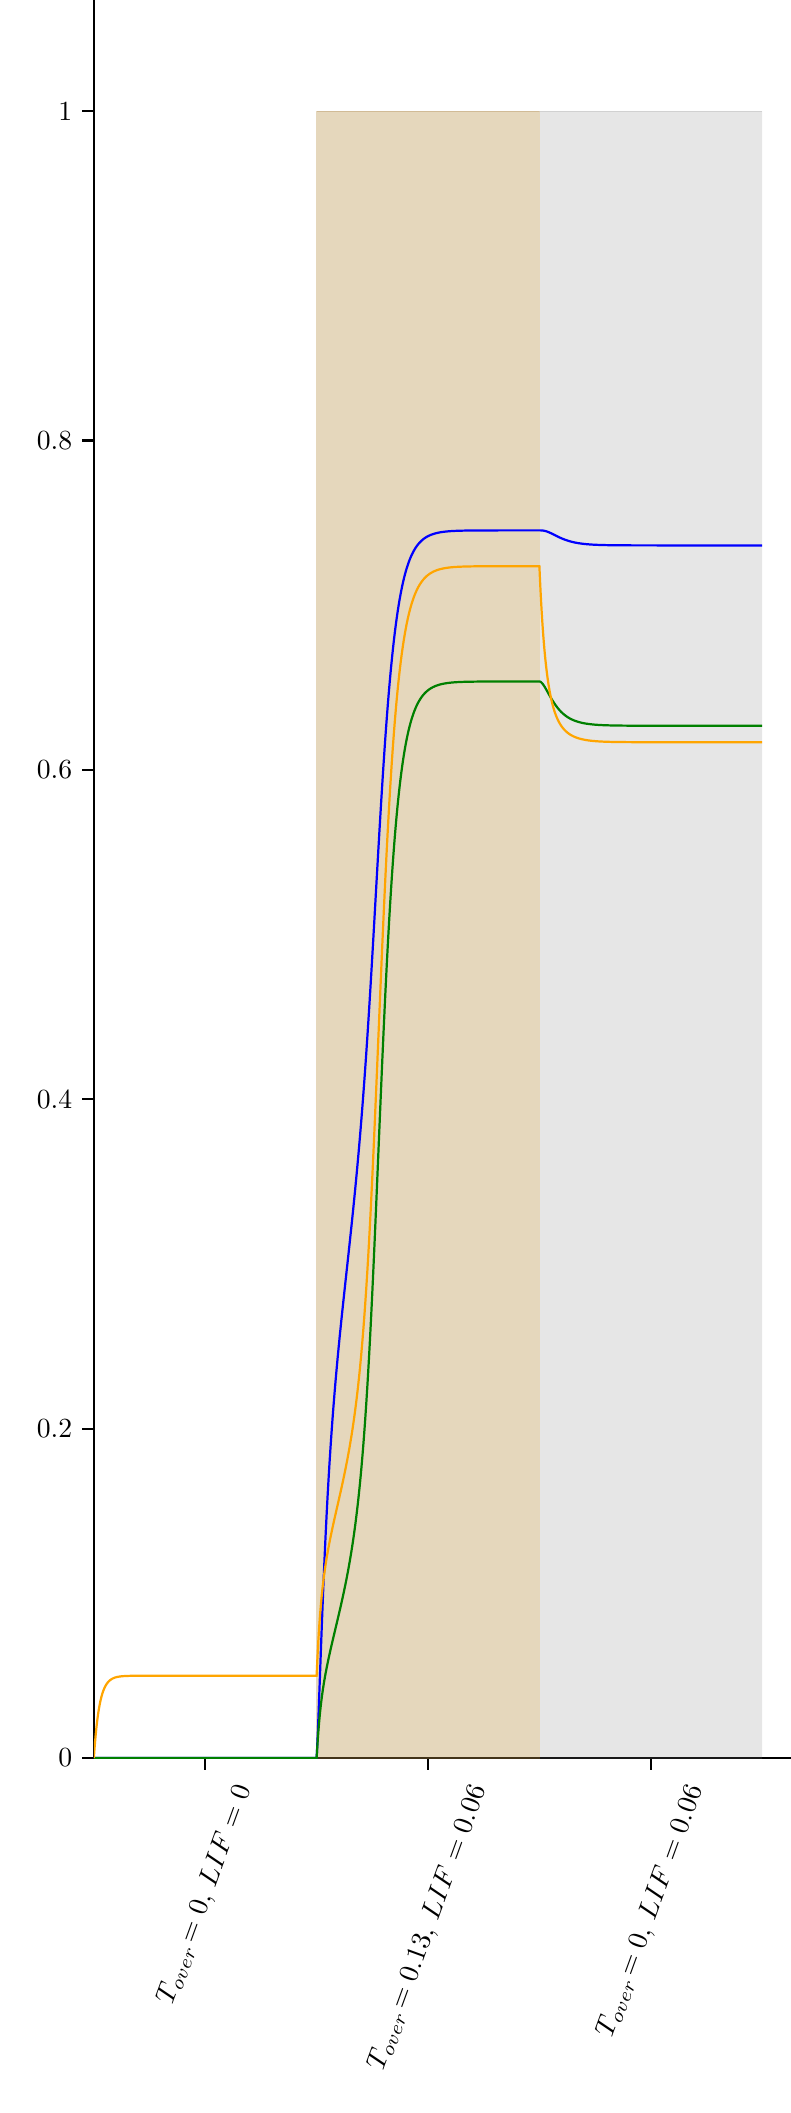
\begin{tikzpicture}[baseline]

\definecolor{darkgray176}{RGB}{176,176,176}
\definecolor{gray}{RGB}{128,128,128}
\definecolor{green}{RGB}{0,128,0}
\definecolor{lightgray204}{RGB}{204,204,204}
\definecolor{orange}{RGB}{255,165,0}

\begin{axis}[
 ytick={0,0.2,0.4,0.6,0.8,1},
 x tick label style = {rotate=70},
 y post scale=3, 
 transpose legend,
legend cell align={left},
legend style={
  fill opacity=0.8,
  draw opacity=1,
  text opacity=1,
  at={(axis cs:5,1.1)},
  anchor=south west,
    legend columns=4,
    /tikz/every even column/.append style={column sep=1.0cm},,
  draw=lightgray204
},
tick align=outside,
tick pos=left,
x grid style={darkgray176},
xmin=0, xmax=120,
xtick style={color=black},
xtick={20,60,100},
xticklabels={
  {\(\displaystyle T_\text{over}\!=0\), \(\displaystyle \text{LIF}=0\)},
  {\(\displaystyle T_\text{over}\!=0.13\), \(\displaystyle \text{LIF}=0.06\)},
  {\(\displaystyle T_\text{over}\!=0\), \(\displaystyle \text{LIF}=0.06\)}
},
y grid style={darkgray176},
ymin=0, ymax=1.05,
ytick style={color=black}
]
\path [draw=orange, fill=orange, opacity=0.2]
(axis cs:40,0)
--(axis cs:40,1)
--(axis cs:80,1)
--(axis cs:80,0)
--cycle;

\path [draw=gray, fill=gray, opacity=0.2]
(axis cs:40,0)
--(axis cs:40,1)
--(axis cs:120,1)
--(axis cs:120,0)
--cycle;

\addplot [thick, blue]
table {%
0 0
0.0001 0
0.0011 0
0.0111 0
0.1111 0
0.2111 0
0.3111 0
0.4111 0
0.5111 0
0.6111 0
0.7111 0
0.8111 0
0.9111 0
1.0111 0
1.1111 0
1.2111 0
1.3111 0
1.4111 0
1.5111 0
1.6111 0
1.7111 0
1.8111 0
1.9111 0
2.0111 0
2.1111 0
2.2111 0
2.3111 0
2.4111 0
2.5111 0
2.6111 0
2.7111 0
2.8111 0
2.9111 0
3.0111 0
3.1111 0
3.2111 0
3.3111 0
3.4111 0
3.5111 0
3.6111 0
3.7111 0
3.8111 0
3.9111 0
4.0111 0
4.1111 0
4.2111 0
4.3111 0
4.4111 0
4.5111 0
4.6111 0
4.7111 0
4.8111 0
4.9111 0
5.0111 0
5.1111 0
5.2111 0
5.3111 0
5.4111 0
5.5111 0
5.6111 0
5.7111 0
5.8111 0
5.9111 0
6.0111 0
6.1111 0
6.21109999999999 0
6.31109999999999 0
6.41109999999999 0
6.51109999999999 0
6.61109999999999 0
6.71109999999999 0
6.81109999999999 0
6.91109999999999 0
7.01109999999999 0
7.11109999999999 0
7.21109999999999 0
7.31109999999999 0
7.41109999999999 0
7.51109999999999 0
7.61109999999999 0
7.71109999999999 0
7.81109999999999 0
7.91109999999999 0
8.01109999999999 0
8.11109999999999 0
8.21109999999999 0
8.31109999999999 0
8.41109999999999 0
8.51109999999999 0
8.61109999999999 0
8.71109999999999 0
8.81109999999999 0
8.91109999999999 0
9.01109999999998 0
9.11109999999998 0
9.21109999999998 0
9.31109999999998 0
9.41109999999998 0
9.51109999999998 0
9.61109999999998 0
9.71109999999998 0
9.81109999999998 0
9.91109999999998 0
10.0111 0
10.1111 0
10.2111 0
10.3111 0
10.4111 0
10.5111 0
10.6111 0
10.7111 0
10.8111 0
10.9111 0
11.0111 0
11.1111 0
11.2111 0
11.3111 0
11.4111 0
11.5111 0
11.6111 0
11.7111 0
11.8111 0
11.9111 0
12.0111 0
12.1111 0
12.2111 0
12.3111 0
12.4111 0
12.5111 0
12.6111 0
12.7111 0
12.8111 0
12.9111 0
13.0111 0
13.1111 0
13.2111 0
13.3111 0
13.4111 0
13.5111 0
13.6111 0
13.7111 0
13.8111 0
13.9111 0
14.0111 0
14.1111 0
14.2111 0
14.3111 0
14.4111 0
14.5111 0
14.6111 0
14.7111 0
14.8111 0
14.9111 0
15.0111 0
15.1111 0
15.2111 0
15.3111 0
15.4111 0
15.5111 0
15.6111 0
15.7111 0
15.8111 0
15.9111 0
16.0111 0
16.1111 0
16.2111 0
16.3111 0
16.4111 0
16.5111 0
16.6111 0
16.7111 0
16.8111 0
16.9111 0
17.0111 0
17.1111 0
17.2111 0
17.3111 0
17.4111 0
17.5111 0
17.6111 0
17.7111 0
17.8111 0
17.9111 0
18.0111 0
18.1111 0
18.2111 0
18.3111 0
18.4111 0
18.5111 0
18.6111 0
18.7111 0
18.8111 0
18.9111 0
19.0111 0
19.1111 0
19.2111 0
19.3111 0
19.4111 0
19.5111 0
19.6111 0
19.7111 0
19.8111 0
19.9111 0
20.0111 0
20.1111 0
20.2111 0
20.3111 0
20.4111 0
20.5111 0
20.6111 0
20.7111 0
20.8111 0
20.9111 0
21.0111 0
21.1111 0
21.2111 0
21.3111 0
21.4111 0
21.5111 0
21.6111 0
21.7111 0
21.8111 0
21.9111 0
22.0111 0
22.1111 0
22.2111 0
22.3111 0
22.4111000000001 0
22.5111000000001 0
22.6111000000001 0
22.7111000000001 0
22.8111000000001 0
22.9111000000001 0
23.0111000000001 0
23.1111000000001 0
23.2111000000001 0
23.3111000000001 0
23.4111000000001 0
23.5111000000001 0
23.6111000000001 0
23.7111000000001 0
23.8111000000001 0
23.9111000000001 0
24.0111000000001 0
24.1111000000001 0
24.2111000000001 0
24.3111000000001 0
24.4111000000001 0
24.5111000000001 0
24.6111000000001 0
24.7111000000001 0
24.8111000000001 0
24.9111000000001 0
25.0111000000001 0
25.1111000000001 0
25.2111000000001 0
25.3111000000001 0
25.4111000000001 0
25.5111000000001 0
25.6111000000001 0
25.7111000000001 0
25.8111000000001 0
25.9111000000001 0
26.0111000000001 0
26.1111000000001 0
26.2111000000001 0
26.3111000000001 0
26.4111000000001 0
26.5111000000001 0
26.6111000000001 0
26.7111000000001 0
26.8111000000001 0
26.9111000000001 0
27.0111000000001 0
27.1111000000001 0
27.2111000000001 0
27.3111000000001 0
27.4111000000001 0
27.5111000000001 0
27.6111000000001 0
27.7111000000001 0
27.8111000000001 0
27.9111000000001 0
28.0111000000001 0
28.1111000000001 0
28.2111000000001 0
28.3111000000001 0
28.4111000000001 0
28.5111000000001 0
28.6111000000001 0
28.7111000000001 0
28.8111000000001 0
28.9111000000001 0
29.0111000000001 0
29.1111000000001 0
29.2111000000001 0
29.3111000000001 0
29.4111000000002 0
29.5111000000002 0
29.6111000000002 0
29.7111000000002 0
29.8111000000002 0
29.9111000000002 0
30.0111000000002 0
30.1111000000002 0
30.2111000000002 0
30.3111000000002 0
30.4111000000002 0
30.5111000000002 0
30.6111000000002 0
30.7111000000002 0
30.8111000000002 0
30.9111000000002 0
31.0111000000002 0
31.1111000000002 0
31.2111000000002 0
31.3111000000002 0
31.4111000000002 0
31.5111000000002 0
31.6111000000002 0
31.7111000000002 0
31.8111000000002 0
31.9111000000002 0
32.0111000000002 0
32.1111000000002 0
32.2111000000002 0
32.3111000000002 0
32.4111000000002 0
32.5111000000002 0
32.6111000000002 0
32.7111000000002 0
32.8111000000002 0
32.9111000000002 0
33.0111000000002 0
33.1111000000002 0
33.2111000000002 0
33.3111000000002 0
33.4111000000002 0
33.5111000000002 0
33.6111000000002 0
33.7111000000002 0
33.8111000000002 0
33.9111000000002 0
34.0111000000002 0
34.1111000000002 0
34.2111000000002 0
34.3111000000002 0
34.4111000000002 0
34.5111000000002 0
34.6111000000002 0
34.7111000000002 0
34.8111000000002 0
34.9111000000002 0
35.0111000000002 0
35.1111000000002 0
35.2111000000002 0
35.3111000000002 0
35.4111000000002 0
35.5111000000002 0
35.6111000000002 0
35.7111000000002 0
35.8111000000002 0
35.9111000000002 0
36.0111000000002 0
36.1111000000002 0
36.2111000000002 0
36.3111000000002 0
36.4111000000002 0
36.5111000000002 0
36.6111000000002 0
36.7111000000003 0
36.8111000000003 0
36.9111000000003 0
37.0111000000003 0
37.1111000000003 0
37.2111000000003 0
37.3111000000003 0
37.4111000000003 0
37.5111000000003 0
37.6111000000003 0
37.7111000000003 0
37.8111000000003 0
37.9111000000003 0
38.0111000000003 0
38.1111000000003 0
38.2111000000003 0
38.3111000000003 0
38.4111000000003 0
38.5111000000003 0
38.6111000000003 0
38.7111000000003 0
38.8111000000003 0
38.9111000000003 0
39.0111000000003 0
39.1111000000003 0
39.2111000000003 0
39.3111000000003 0
39.4111000000003 0
39.5111000000003 0
39.6111000000003 0
39.7111000000003 0
39.8111000000003 0
39.9111000000003 0
40 0
40 0
40.0115520585893 0.000702357776229193
40.1115520585893 0.0074726152252318
40.2115520585893 0.0152326552734989
40.3115520585893 0.0236853438983936
40.4115520585893 0.0325929667982848
40.5115520585893 0.0417667251595415
40.6115520585893 0.0510581342136438
40.7115520585893 0.0603518591775368
40.8115520585893 0.0695596961856092
40.9115520585893 0.0786155064156931
41.0115520585893 0.0874709655021017
41.1115520585893 0.0960920178261974
41.2115520585893 0.104455939847231
41.3115520585893 0.112548926008486
41.4115520585893 0.120364118695471
41.5115520585893 0.127900011661253
41.6115520585893 0.135159164512532
41.7115520585893 0.142147174036876
41.8115520585893 0.148871856013803
41.9115520585893 0.155342598416931
42.0115520585893 0.16156985341549
42.1115520585893 0.167564741254576
42.2115520585893 0.173338743942927
42.3115520585893 0.178903470759787
42.4115520585893 0.184270480988983
42.5115520585893 0.189451152088039
42.6115520585893 0.194456583791768
42.7115520585893 0.199297530515509
42.8115520585893 0.203984355936043
42.9115520585893 0.208527004851282
43.0115520585893 0.212934988406314
43.1115520585893 0.217217379567723
43.2115520585893 0.221382816366856
43.3115520585893 0.225439510945817
43.4115520585893 0.229395262851727
43.5115520585893 0.233257475354954
43.6115520585893 0.237033173831516
43.7115520585893 0.240729025461431
43.8115520585893 0.244351359663921
43.9115520585893 0.247906188825242
44.0115520585893 0.251399228982274
44.1115520585893 0.254835920210237
44.2115520585893 0.258221446530283
44.3115520585893 0.261560755205793
44.4115520585894 0.264858575337706
44.5115520585894 0.268119435701444
44.6115520585894 0.271347681792744
44.7115520585894 0.274547492068387
44.8115520585894 0.277722893381702
44.9115520585894 0.280877775622589
45.0115520585894 0.28401590557857
45.1115520585894 0.287140940037494
45.2115520585894 0.290256438154526
45.3115520585894 0.29336587310633
45.4115520585894 0.296472643054136
45.5115520585894 0.299580081434925
45.6115520585894 0.302691466596438
45.7115520585894 0.305810030787212
45.8115520585894 0.30893896850749
45.9115520585894 0.312081444220649
46.0115520585894 0.31524059941785
46.1115520585894 0.318419559020875
46.2115520585894 0.321621437099676
46.3115520585894 0.324849341871944
46.4115520585894 0.328106379942151
46.5115520585894 0.331395659726862
46.6115520585894 0.334720294001962
46.7115520585894 0.338083401495621
46.8115520585894 0.341488107438617
46.9115520585894 0.344937542971205
47.0115520585894 0.348434843293205
47.1115520585894 0.351983144431856
47.2115520585894 0.355585578490583
47.3115520585894 0.359245267231706
47.4115520585894 0.362965313838027
47.5115520585894 0.366748792692894
47.6115520585894 0.370598737016871
47.7115520585894 0.374518124202544
47.8115520585894 0.378509858698689
47.9115520585894 0.382576752312339
48.0115520585894 0.386721501823777
48.1115520585894 0.390946663846615
48.2115520585894 0.395254626914358
48.3115520585894 0.399647580837373
48.4115520585894 0.404127483450862
48.5115520585894 0.408696024965466
48.6115520585894 0.413354590237112
48.7115520585894 0.418104219389957
48.8115520585894 0.422945567353249
48.9115520585894 0.427878863005311
49.0115520585894 0.432903868750267
49.1115520585894 0.438019841478402
49.2115520585894 0.4432254959711
49.3115520585894 0.448518971896841
49.4115520585894 0.453897805596524
49.5115520585894 0.459358907865179
49.6115520585894 0.464898548895458
49.7115520585894 0.470512351450517
49.8115520585894 0.476195293177835
49.9115520585894 0.481941718762609
50.0115520585894 0.487745362355535
50.1115520585894 0.493599380405172
50.2115520585894 0.499496394693761
50.3115520585894 0.505428545034344
50.4115520585894 0.511387550755127
50.5115520585894 0.517364779793086
50.6115520585894 0.523351323960215
50.7115520585894 0.529338078747104
50.8115520585894 0.535315825899665
50.9115520585894 0.541275316951322
51.0115520585894 0.547207355914563
51.1115520585894 0.553102879427824
51.2115520585894 0.558953032806928
51.3115520585894 0.564749240652736
51.4115520585895 0.570483270904163
51.5115520585895 0.57614729148363
51.6115520585895 0.581733918946271
51.7115520585895 0.587236258802071
51.8115520585895 0.592647937421069
51.9115520585895 0.597963125647682
52.0115520585895 0.603176554435624
52.1115520585895 0.608283522966743
52.2115520585895 0.613279899834518
52.3115520585895 0.618162117956984
52.4115520585895 0.622927163936699
52.5115520585895 0.627572562610557
52.6115520585895 0.632096357533481
52.7115520585895 0.636497088121673
52.8115520585895 0.640773764147085
52.9115520585895 0.644925838229213
53.0115520585895 0.648953176916613
53.1115520585895 0.652856030891915
53.2115520585895 0.656635004773145
53.3115520585895 0.660291026923049
53.4115520585895 0.663825319618505
53.5115520585895 0.667239369875361
53.6115520585895 0.67053490117098
53.7115520585895 0.673713846258033
53.8115520585895 0.676778321219066
53.9115520585895 0.679730600872057
54.0115520585895 0.68257309560266
54.1115520585895 0.685308329668931
54.2115520585895 0.687938920998704
54.3115520585895 0.690467562478222
54.4115520585895 0.692897004712793
54.5115520585895 0.695230040225642
54.6115520585895 0.69746948904961
54.7115520585895 0.699618185657337
54.8115520585895 0.701678967168933
54.9115520585895 0.70365466277139
55.0115520585895 0.705548084280957
55.1115520585895 0.707362017778077
55.2115520585895 0.709099216244002
55.3115520585895 0.710762393128726
55.4115520585895 0.712354216781155
55.5115520585895 0.713877305674307
55.6115520585895 0.715334224360725
55.7115520585895 0.716727480096005
55.8115520585895 0.718059520071307
55.9115520585895 0.719332729198872
56.0115520585895 0.720549428397787
56.1115520585895 0.721711873330543
56.2115520585895 0.722822253544159
56.3115520585895 0.723882691972876
56.4115520585895 0.724895244762552
56.5115520585895 0.72586190137991
56.6115520585895 0.726784584972709
56.7115520585895 0.727665152949653
56.8115520585895 0.728505397751526
56.9115520585895 0.729307047787474
57.0115520585895 0.730071768512734
57.1115520585895 0.730801163626272
57.2115520585895 0.73149677636884
57.3115520585895 0.732160090903852
57.4115520585895 0.73279253376526
57.5115520585895 0.733395475358215
57.6115520585895 0.733970231499808
57.7115520585895 0.734518064988571
57.8115520585895 0.735040187192675
57.9115520585895 0.735537759647936
58.0115520585895 0.736011895657769
58.1115520585895 0.736463661888245
58.2115520585895 0.736894079952222
58.3115520585895 0.737304127977375
58.4115520585895 0.737694742153623
58.5115520585896 0.738066818256148
58.6115520585896 0.738421213140731
58.7115520585896 0.73875874620873
58.8115520585896 0.739080200839414
58.9115520585896 0.739386325787881
59.0115520585896 0.739677836547078
59.1115520585896 0.739955416672854
59.2115520585896 0.740219719071214
59.3115520585896 0.740471367247256
59.4115520585896 0.740710956515464
59.5115520585896 0.740939055171266
59.6115520585896 0.741156205623923
59.7115520585896 0.741362925490986
59.8115520585896 0.741559708654677
59.9115520585896 0.741747026280682
60.0115520585896 0.741925327799926
60.1115520585896 0.742095041853994
60.2115520585896 0.742256577204933
60.3115520585896 0.742410323610205
60.4115520585896 0.742556652663655
60.5115520585896 0.742695918603334
60.6115520585896 0.742828459087089
60.7115520585896 0.742954595936849
60.8115520585896 0.743074635852518
60.9115520585896 0.743188871096441
61.0115520585896 0.743297580149362
61.1115520585896 0.743401028338838
61.2115520585896 0.74349946844104
61.3115520585896 0.743593141256857
61.4115520585896 0.743682276163236
61.5115520585896 0.743767091640659
61.6115520585896 0.743847795777625
61.7115520585896 0.743924586753035
61.8115520585896 0.743997653297301
61.9115520585896 0.744067175133024
62.0115520585896 0.744133323396048
62.1115520585896 0.744196261037663
62.2115520585896 0.74425614320874
62.3115520585896 0.744313117626511
62.4115520585896 0.744367324924744
62.5115520585896 0.744418898987972
62.6115520585896 0.744467967270473
62.7115520585896 0.744514651100637
62.8115520585896 0.744559065971348
62.9115520585896 0.744601321816977
63.0115520585896 0.744641523277585
63.1115520585896 0.744679769950865
63.2115520585896 0.744716156632392
63.3115520585896 0.744750773544679
63.4115520585896 0.744783706555536
63.5115520585896 0.744815037386222
63.6115520585896 0.744844843809833
63.7115520585896 0.744873199840375
63.8115520585896 0.744900175912937
63.9115520585896 0.744925839055374
64.0115520585896 0.744950253051882
64.1115520585896 0.744973478598836
64.2115520585896 0.744995573453253
64.3115520585896 0.745016592574203
64.4115520585896 0.745036588257511
64.5115520585896 0.745055610264057
64.6115520585896 0.745073705941952
64.7115520585896 0.74509092034291
64.8115520585896 0.74510729633305
64.9115520585896 0.745122874698411
65.0115520585896 0.745137694245425
65.1115520585896 0.745151791896576
65.2115520585896 0.745165202781473
65.3115520585896 0.74517796032357
65.4115520585895 0.745190096322706
65.5115520585895 0.745201641033696
65.6115520585895 0.745212623241134
65.7115520585895 0.745223070330609
65.8115520585895 0.745233008356484
65.9115520585895 0.745242462106419
66.0115520585895 0.745251455162774
66.1115520585895 0.745260009961068
66.2115520585895 0.7452681478456
66.3115520585895 0.745275889122398
66.4115520585895 0.745283253109607
66.5115520585895 0.745290258185443
66.6115520585895 0.745296921833827
66.7115520585895 0.745303260687815
66.8115520585895 0.74530929057093
66.9115520585895 0.745315026536484
67.0115520585895 0.745320482905009
67.1115520585895 0.745325673299865
67.2115520585894 0.74533061068113
67.3115520585894 0.745335307377842
67.4115520585894 0.745339775118685
67.5115520585894 0.745344025061179
67.6115520585894 0.745348067819461
67.7115520585894 0.745351913490716
67.8115520585894 0.745355571680322
67.9115520585894 0.745359051525783
68.0115520585894 0.745362361719489
68.1115520585894 0.745365510530381
68.2115520585894 0.745368505824559
68.3115520585894 0.745371355084887
68.4115520585894 0.745374065429647
68.5115520585894 0.745376643630294
68.6115520585894 0.745379096128334
68.7115520585894 0.745381429051391
68.8115520585894 0.745383648228495
68.9115520585894 0.745385759204616
69.0115520585893 0.745387767254501
69.1115520585893 0.745389677395836
69.2115520585893 0.745391494401763
69.3115520585893 0.745393222812794
69.4115520585893 0.745394866948141
69.5115520585893 0.745396430916498
69.6115520585893 0.745397918626294
69.7115520585893 0.745399333795454
69.8115520585893 0.745400679960675
69.9115520585893 0.745401960486263
70.0115520585893 0.745403178572524
70.1115520585893 0.745404337263764
70.2115520585893 0.745405439455885
70.3115520585893 0.745406487903618
70.4115520585893 0.745407485227405
70.5115520585893 0.745408433919938
70.6115520585893 0.745409336352394
70.7115520585892 0.745410194780346
70.8115520585892 0.745411011349407
70.9115520585892 0.745411788100584
71.0115520585892 0.745412526975378
71.1115520585892 0.745413229820634
71.2115520585892 0.745413898393157
71.3115520585892 0.745414534364096
71.4115520585892 0.745415139323125
71.5115520585892 0.745415714782409
71.6115520585892 0.745416262180388
71.7115520585892 0.745416782885367
71.8115520585892 0.745417278198935
71.9115520585892 0.745417749359221
72.0115520585892 0.745418197543982
72.1115520585892 0.745418623873552
72.2115520585892 0.745419029413639
72.3115520585892 0.745419415177986
72.4115520585892 0.745419782130908
72.5115520585891 0.7454201311897
72.6115520585891 0.745420463226929
72.7115520585891 0.745420779072617
72.8115520585891 0.745421079516313
72.9115520585891 0.745421365309066
73.0115520585891 0.745421637165304
73.1115520585891 0.745421895764619
73.2115520585891 0.745422141753465
73.3115520585891 0.745422375746772
73.4115520585891 0.745422598329489
73.5115520585891 0.745422810058037
73.6115520585891 0.745423011461709
73.7115520585891 0.745423203043985
73.8115520585891 0.745423385283796
73.9115520585891 0.745423558636719
74.0115520585891 0.745423723536115
74.1115520585891 0.745423880394214
74.211552058589 0.745424029603144
74.311552058589 0.745424171535911
74.411552058589 0.745424306547332
74.511552058589 0.745424434974925
74.611552058589 0.745424557139745
74.711552058589 0.745424673347194
74.811552058589 0.74542478388778
74.911552058589 0.745424889037846
75.011552058589 0.745424989060259
75.111552058589 0.745425084205068
75.211552058589 0.745425174710127
75.311552058589 0.745425260801694
75.411552058589 0.74542534269499
75.511552058589 0.745425420594745
75.611552058589 0.745425494695703
75.711552058589 0.745425565183111
75.811552058589 0.745425632233185
75.911552058589 0.745425696013546
76.0115520585889 0.745425756683641
76.1115520585889 0.745425814395143
76.2115520585889 0.745425869292328
76.3115520585889 0.745425921512435
76.4115520585889 0.745425971186013
76.5115520585889 0.745426018437244
76.6115520585889 0.745426063384254
76.7115520585889 0.745426106139407
76.8115520585889 0.745426146809592
76.9115520585889 0.745426185496481
77.0115520585889 0.74542622229679
77.1115520585889 0.745426257302519
77.2115520585889 0.74542629060118
77.3115520585889 0.745426322276021
77.4115520585889 0.745426352406225
77.5115520585889 0.745426381067119
77.6115520585889 0.745426408330352
77.7115520585889 0.745426434264084
77.8115520585888 0.745426458933147
77.9115520585888 0.745426482399212
78.0115520585888 0.745426504720946
78.1115520585888 0.745426525954151
78.2115520585888 0.745426546151909
78.3115520585888 0.745426565364716
78.4115520585888 0.745426583640602
78.5115520585888 0.745426601025256
78.6115520585888 0.74542661756214
78.7115520585888 0.745426633292596
78.8115520585888 0.745426648255949
78.9115520585888 0.745426662489607
79.0115520585888 0.745426676029155
79.1115520585888 0.745426688908441
79.2115520585888 0.745426701159662
79.3115520585888 0.745426712813448
79.4115520585888 0.74542672389893
79.5115520585887 0.745426734443825
79.6115520585887 0.745426744474492
79.7115520585887 0.74542675401601
79.8115520585887 0.745426763092231
79.9115520585887 0.745426771725846
80 0.745426779010556
80 0.745426779010556
80.1 0.745426229473644
80.2 0.745422577761376
80.3 0.745413342269621
80.4 0.745396629407156
80.5 0.745371046601449
80.6 0.745335625628684
80.7 0.745289755218656
80.8 0.745233121979513
80.8999999999999 0.745165658773219
80.9999999999999 0.745087499751239
81.0999999999999 0.744998941332083
81.1999999999999 0.744900408468727
81.2999999999999 0.744792425614975
81.3999999999999 0.744675591856023
81.4999999999999 0.744550559720234
81.5999999999999 0.744418017236612
81.6999999999999 0.744278672846112
81.7999999999999 0.744133242814866
81.8999999999999 0.743982440833965
81.9999999999999 0.743826969523807
82.0999999999999 0.743667513591424
82.1999999999999 0.743504734416807
82.2999999999999 0.743339265869377
82.3999999999999 0.743171711178366
82.4999999999999 0.743002640701455
82.5999999999999 0.742832590454409
82.6999999999998 0.742662061281144
82.7999999999998 0.742491518558496
82.8999999999998 0.742321392343374
82.9999999999998 0.742152077881866
83.0999999999998 0.741983936410511
83.1999999999998 0.741817296189408
83.2999999999998 0.741652453715208
83.3999999999998 0.741489675069482
83.4999999999998 0.741329197364472
83.5999999999998 0.741171230254065
83.6999999999998 0.74101595748283
83.7999999999998 0.740863538450468
83.8999999999998 0.740714109772846
83.9999999999998 0.740567786824202
84.0999999999998 0.740424665248014
84.1999999999998 0.740284822426581
84.2999999999998 0.740148318901515
84.3999999999997 0.740015199739243
84.4999999999997 0.739885495837203
84.5999999999997 0.739759225167759
84.6999999999997 0.739636393958029
84.7999999999997 0.73951699780476
84.8999999999997 0.739401022724173
84.9999999999997 0.739288446137388
85.0999999999997 0.739179237792526
85.1999999999997 0.739073360625055
85.2999999999997 0.738970771558249
85.3999999999997 0.738871422245916
85.4999999999997 0.738775259759714
85.5999999999997 0.738682227223533
85.6999999999997 0.738592264397488
85.7999999999997 0.738505308214137
85.8999999999997 0.738421293269517
85.9999999999997 0.738340152271623
86.0999999999997 0.738261816448866
86.1999999999996 0.738186215921041
86.2999999999996 0.73811328003522
86.3999999999996 0.738042937668945
86.4999999999996 0.737975117502976
86.5999999999996 0.737909748265774
86.6999999999996 0.737846758951782
86.7999999999996 0.737786079015489
86.8999999999996 0.737727638543131
86.9999999999996 0.737671368403802
87.0999999999996 0.737617200381641
87.1999999999996 0.737565067290652
87.2999999999996 0.737514903073639
87.3999999999996 0.737466642886612
87.4999999999996 0.73742022316996
87.5999999999996 0.737375581707583
87.6999999999996 0.737332657675099
87.7999999999996 0.73729139167815
87.8999999999996 0.737251725781776
87.9999999999995 0.737213603531741
88.0999999999995 0.737176969968627
88.1999999999995 0.737141771635449
88.2999999999995 0.737107956579498
88.3999999999995 0.737075474349041
88.4999999999995 0.73704427598547
88.5999999999995 0.737014314011438
88.6999999999995 0.736985542415475
88.7999999999995 0.736957916633531
88.8999999999995 0.736931393527861
88.9999999999995 0.736905931363616
89.0999999999995 0.736881489783499
89.1999999999995 0.736858029780767
89.2999999999995 0.736835513670881
89.3999999999995 0.736813905062042
89.4999999999995 0.736793168824846
89.5999999999995 0.736773271061258
89.6999999999994 0.736754179073094
89.7999999999994 0.736735861330169
89.8999999999994 0.736718287438258
89.9999999999994 0.736701428107003
90.0999999999994 0.736685255117876
90.1999999999994 0.736669741292309
90.2999999999994 0.736654860460069
90.3999999999994 0.736640587427956
90.4999999999994 0.736626897948912
90.5999999999994 0.736613768691566
90.6999999999994 0.736601177210296
90.7999999999994 0.736589101915834
90.8999999999994 0.736577522046449
90.9999999999994 0.736566417639753
91.0999999999994 0.736555769505127
91.1999999999994 0.736545559196817
91.2999999999994 0.736535768987689
91.3999999999994 0.736526381843666
91.4999999999993 0.736517381398854
91.5999999999993 0.736508751931352
91.6999999999993 0.736500478339757
91.7999999999993 0.736492546120358
91.8999999999993 0.736484941345011
91.9999999999993 0.736477650639698
92.0999999999993 0.73647066116375
92.1999999999993 0.736463960589745
92.2999999999993 0.736457537084046
92.3999999999993 0.736451379287987
92.4999999999993 0.73644547629969
92.5999999999993 0.736439817656493
92.6999999999993 0.736434393317984
92.7999999999993 0.736429193649626
92.8999999999993 0.736424209406954
92.9999999999993 0.736419431720332
93.0999999999993 0.736414852080259
93.1999999999992 0.736410462323204
93.2999999999992 0.736406254617955
93.3999999999992 0.736402221452467
93.4999999999992 0.736398355621208
93.5999999999992 0.736394650212956
93.6999999999992 0.736391098599072
93.7999999999992 0.736387694422203
93.8999999999992 0.736384431585416
93.9999999999992 0.736381304241746
94.0999999999992 0.736378306784146
94.1999999999992 0.736375433835817
94.2999999999992 0.736372680240921
94.3999999999992 0.736370041055643
94.4999999999992 0.73636751153961
94.5999999999992 0.73636508714764
94.6999999999992 0.736362763521817
94.7999999999992 0.736360536483876
94.8999999999992 0.73635840202789
94.9999999999991 0.736356356313244
95.0999999999991 0.736354395657889
95.1999999999991 0.736352516531868
95.2999999999991 0.736350715551093
95.3999999999991 0.736348989471374
95.4999999999991 0.736347335182691
95.5999999999991 0.73634574970369
95.6999999999991 0.736344230176403
95.7999999999991 0.736342773861182
95.8999999999991 0.736341378131834
95.9999999999991 0.736340040470955
96.0999999999991 0.736338758465456
96.1999999999991 0.736337529802262
96.2999999999991 0.736336352264196
96.3999999999991 0.73633522372602
96.4999999999991 0.736334142150647
96.5999999999991 0.736333105585501
96.6999999999991 0.736332112159026
96.799999999999 0.736331160077341
96.899999999999 0.736330247621031
96.999999999999 0.736329373142063
97.099999999999 0.736328535060839
97.199999999999 0.736327731863364
97.299999999999 0.736326962098526
97.399999999999 0.736326224375498
97.499999999999 0.736325517361238
97.599999999999 0.736324839778096
97.699999999999 0.736324190401518
97.799999999999 0.736323568057846
97.899999999999 0.736322971622207
97.999999999999 0.73632240001649
98.099999999999 0.736321852207406
98.199999999999 0.736321327204631
98.299999999999 0.736320824059018
98.399999999999 0.736320341860892
98.4999999999989 0.736319879738411
98.5999999999989 0.736319436855992
98.6999999999989 0.736319012412811
98.7999999999989 0.736318605641352
98.8999999999989 0.736318215806031
98.9999999999989 0.736317842201864
99.0999999999989 0.736317484153197
99.1999999999989 0.736317141012489
99.2999999999989 0.736316812159141
99.3999999999989 0.736316496998378
99.4999999999989 0.736316194960174
99.5999999999989 0.736315905498225
99.6999999999989 0.736315628088962
99.7999999999989 0.736315362230603
99.8999999999989 0.736315107442253
99.9999999999989 0.736314863263028
100.099999999999 0.73631462925123
100.199999999999 0.736314404983543
100.299999999999 0.736314190054271
100.399999999999 0.736313984074607
100.499999999999 0.736313786671927
100.599999999999 0.736313597489117
100.699999999999 0.736313416183931
100.799999999999 0.736313242428368
100.899999999999 0.736313075908083
100.999999999999 0.736312916321816
101.099999999999 0.73631276338085
101.199999999999 0.736312616808485
101.299999999999 0.736312476339545
101.399999999999 0.73631234171989
101.499999999999 0.736312212705962
101.599999999999 0.736312089064344
101.699999999999 0.736311970571336
101.799999999999 0.736311857012552
101.899999999999 0.736311748182533
101.999999999999 0.736311643884372
102.099999999999 0.736311543929364
102.199999999999 0.736311448136658
102.299999999999 0.736311356332934
102.399999999999 0.73631126835209
102.499999999999 0.736311184034937
102.599999999999 0.736311103228917
102.699999999999 0.736311025787822
102.799999999999 0.736310951571535
102.899999999999 0.736310880445771
102.999999999999 0.736310812281835
103.099999999999 0.736310746956395
103.199999999999 0.736310684351251
103.299999999999 0.736310624353126
103.399999999999 0.736310566853459
103.499999999999 0.736310511748211
103.599999999999 0.736310458937674
103.699999999999 0.736310408326293
103.799999999999 0.73631035982249
103.899999999999 0.736310313338502
103.999999999999 0.73631026879022
104.099999999999 0.736310226097037
104.199999999999 0.736310185181703
104.299999999999 0.736310145970186
104.399999999999 0.736310108391534
104.499999999999 0.736310072377751
104.599999999999 0.736310037863673
104.699999999999 0.736310004786849
104.799999999999 0.736309973087429
104.899999999999 0.736309942708053
104.999999999999 0.736309913593753
105.099999999999 0.736309885691847
105.199999999999 0.736309858951849
105.299999999999 0.736309833325375
105.399999999999 0.736309808766053
105.499999999999 0.736309785229446
105.599999999999 0.736309762672966
105.699999999999 0.736309741055796
105.799999999999 0.736309720338822
105.899999999999 0.736309700484558
105.999999999999 0.736309681457079
106.099999999999 0.736309663221954
106.199999999999 0.736309645746188
106.299999999999 0.736309628998159
106.399999999998 0.736309612947564
106.499999999998 0.736309597565358
106.599999999998 0.736309582823708
106.699999999998 0.73630956869594
106.799999999998 0.73630955515649
106.899999999998 0.736309542180859
106.999999999998 0.736309529745569
107.099999999998 0.736309517828117
107.199999999998 0.73630950640694
107.299999999998 0.736309495461372
107.399999999998 0.736309484971607
107.499999999998 0.736309474918664
107.599999999998 0.736309465284353
107.699999999998 0.73630945605124
107.799999999998 0.73630944720262
107.899999999998 0.736309438722479
107.999999999998 0.736309430595475
108.099999999998 0.736309422806902
108.199999999998 0.736309415342665
108.299999999998 0.73630940818926
108.399999999998 0.736309401333742
108.499999999998 0.736309394763706
108.599999999998 0.736309388467264
108.699999999998 0.736309382433024
108.799999999998 0.736309376650065
108.899999999998 0.736309371107925
108.999999999998 0.736309365796574
109.099999999998 0.736309360706403
109.199999999998 0.7363093558282
109.299999999998 0.736309351153138
109.399999999998 0.736309346672759
109.499999999998 0.736309342378956
109.599999999998 0.736309338263957
109.699999999998 0.736309334320319
109.799999999998 0.736309330540904
109.899999999998 0.736309326918875
109.999999999998 0.736309323447676
110.099999999998 0.736309320121028
110.199999999998 0.73630931693291
110.299999999998 0.736309313877555
110.399999999998 0.736309310949432
110.499999999998 0.736309308143245
110.599999999998 0.736309305453915
110.699999999998 0.736309302876576
110.799999999998 0.736309300406564
110.899999999998 0.736309298039411
110.999999999998 0.736309295770832
111.099999999998 0.736309293596723
111.199999999998 0.736309291513149
111.299999999998 0.736309289516342
111.399999999998 0.736309287602687
111.499999999998 0.736309285768721
111.599999999998 0.736309284011127
111.699999999998 0.736309282326724
111.799999999998 0.736309280712464
111.899999999998 0.736309279165427
111.999999999998 0.736309277682812
112.099999999998 0.736309276261937
112.199999999998 0.736309274900232
112.299999999998 0.736309273595231
112.399999999998 0.736309272344574
112.499999999998 0.736309271145998
112.599999999998 0.736309269997334
112.699999999998 0.736309268896504
112.799999999998 0.736309267841515
112.899999999998 0.736309266830458
112.999999999998 0.736309265861505
113.099999999998 0.736309264932902
113.199999999998 0.736309264042968
113.299999999998 0.736309263190094
113.399999999998 0.736309262372735
113.499999999998 0.736309261589414
113.599999999998 0.736309260838712
113.699999999998 0.736309260119271
113.799999999998 0.73630925942979
113.899999999998 0.736309258769021
113.999999999998 0.736309258135768
114.099999999998 0.736309257528885
114.199999999998 0.736309256947275
114.299999999998 0.736309256389884
114.399999999998 0.736309255855705
114.499999999998 0.73630925534377
114.599999999998 0.736309254853154
114.699999999998 0.736309254382969
114.799999999998 0.736309253932363
114.899999999998 0.736309253500521
114.999999999998 0.736309253086663
115.099999999998 0.736309252690039
115.199999999998 0.736309252309931
115.299999999998 0.736309251945652
115.399999999998 0.736309251596543
115.499999999998 0.736309251261971
115.599999999998 0.736309250941332
115.699999999998 0.736309250634046
115.799999999998 0.736309250339555
115.899999999998 0.736309250057328
115.999999999998 0.736309249786853
116.099999999998 0.736309249527642
116.199999999998 0.736309249279225
116.299999999998 0.736309249041153
116.399999999998 0.736309248812995
116.499999999998 0.736309248594338
116.599999999998 0.736309248384787
116.699999999998 0.736309248183961
116.799999999998 0.736309247991499
116.899999999998 0.736309247807052
116.999999999998 0.736309247630285
117.099999999998 0.736309247460879
117.199999999998 0.736309247298528
117.299999999998 0.736309247142937
117.399999999998 0.736309246993826
117.499999999998 0.736309246850924
117.599999999998 0.736309246713973
117.699999999998 0.736309246582725
117.799999999998 0.736309246456943
117.899999999998 0.736309246336398
117.999999999998 0.736309246220873
118.099999999998 0.736309246110159
118.199999999998 0.736309246004056
118.299999999998 0.736309245902371
118.399999999998 0.73630924580492
118.499999999998 0.736309245711527
118.599999999998 0.736309245622024
118.699999999998 0.736309245536248
118.799999999998 0.736309245454043
118.899999999998 0.736309245375262
118.999999999998 0.736309245299762
119.099999999998 0.736309245227405
119.199999999998 0.736309245158062
119.299999999998 0.736309245091606
119.399999999998 0.736309245027918
119.499999999998 0.736309244966882
119.599999999998 0.736309244908388
119.699999999998 0.736309244852329
119.799999999998 0.736309244798605
119.899999999998 0.736309244747118
119.999999999998 0.736309244697775
120 0.736309244697775
};
\addplot [thick, green]
table {%
0 0
0.0001 0
0.0011 0
0.0111 0
0.1111 0
0.2111 0
0.3111 0
0.4111 0
0.5111 0
0.6111 0
0.7111 0
0.8111 0
0.9111 0
1.0111 0
1.1111 0
1.2111 0
1.3111 0
1.4111 0
1.5111 0
1.6111 0
1.7111 0
1.8111 0
1.9111 0
2.0111 0
2.1111 0
2.2111 0
2.3111 0
2.4111 0
2.5111 0
2.6111 0
2.7111 0
2.8111 0
2.9111 0
3.0111 0
3.1111 0
3.2111 0
3.3111 0
3.4111 0
3.5111 0
3.6111 0
3.7111 0
3.8111 0
3.9111 0
4.0111 0
4.1111 0
4.2111 0
4.3111 0
4.4111 0
4.5111 0
4.6111 0
4.7111 0
4.8111 0
4.9111 0
5.0111 0
5.1111 0
5.2111 0
5.3111 0
5.4111 0
5.5111 0
5.6111 0
5.7111 0
5.8111 0
5.9111 0
6.0111 0
6.1111 0
6.21109999999999 0
6.31109999999999 0
6.41109999999999 0
6.51109999999999 0
6.61109999999999 0
6.71109999999999 0
6.81109999999999 0
6.91109999999999 0
7.01109999999999 0
7.11109999999999 0
7.21109999999999 0
7.31109999999999 0
7.41109999999999 0
7.51109999999999 0
7.61109999999999 0
7.71109999999999 0
7.81109999999999 0
7.91109999999999 0
8.01109999999999 0
8.11109999999999 0
8.21109999999999 0
8.31109999999999 0
8.41109999999999 0
8.51109999999999 0
8.61109999999999 0
8.71109999999999 0
8.81109999999999 0
8.91109999999999 0
9.01109999999998 0
9.11109999999998 0
9.21109999999998 0
9.31109999999998 0
9.41109999999998 0
9.51109999999998 0
9.61109999999998 0
9.71109999999998 0
9.81109999999998 0
9.91109999999998 0
10.0111 0
10.1111 0
10.2111 0
10.3111 0
10.4111 0
10.5111 0
10.6111 0
10.7111 0
10.8111 0
10.9111 0
11.0111 0
11.1111 0
11.2111 0
11.3111 0
11.4111 0
11.5111 0
11.6111 0
11.7111 0
11.8111 0
11.9111 0
12.0111 0
12.1111 0
12.2111 0
12.3111 0
12.4111 0
12.5111 0
12.6111 0
12.7111 0
12.8111 0
12.9111 0
13.0111 0
13.1111 0
13.2111 0
13.3111 0
13.4111 0
13.5111 0
13.6111 0
13.7111 0
13.8111 0
13.9111 0
14.0111 0
14.1111 0
14.2111 0
14.3111 0
14.4111 0
14.5111 0
14.6111 0
14.7111 0
14.8111 0
14.9111 0
15.0111 0
15.1111 0
15.2111 0
15.3111 0
15.4111 0
15.5111 0
15.6111 0
15.7111 0
15.8111 0
15.9111 0
16.0111 0
16.1111 0
16.2111 0
16.3111 0
16.4111 0
16.5111 0
16.6111 0
16.7111 0
16.8111 0
16.9111 0
17.0111 0
17.1111 0
17.2111 0
17.3111 0
17.4111 0
17.5111 0
17.6111 0
17.7111 0
17.8111 0
17.9111 0
18.0111 0
18.1111 0
18.2111 0
18.3111 0
18.4111 0
18.5111 0
18.6111 0
18.7111 0
18.8111 0
18.9111 0
19.0111 0
19.1111 0
19.2111 0
19.3111 0
19.4111 0
19.5111 0
19.6111 0
19.7111 0
19.8111 0
19.9111 0
20.0111 0
20.1111 0
20.2111 0
20.3111 0
20.4111 0
20.5111 0
20.6111 0
20.7111 0
20.8111 0
20.9111 0
21.0111 0
21.1111 0
21.2111 0
21.3111 0
21.4111 0
21.5111 0
21.6111 0
21.7111 0
21.8111 0
21.9111 0
22.0111 0
22.1111 0
22.2111 0
22.3111 0
22.4111000000001 0
22.5111000000001 0
22.6111000000001 0
22.7111000000001 0
22.8111000000001 0
22.9111000000001 0
23.0111000000001 0
23.1111000000001 0
23.2111000000001 0
23.3111000000001 0
23.4111000000001 0
23.5111000000001 0
23.6111000000001 0
23.7111000000001 0
23.8111000000001 0
23.9111000000001 0
24.0111000000001 0
24.1111000000001 0
24.2111000000001 0
24.3111000000001 0
24.4111000000001 0
24.5111000000001 0
24.6111000000001 0
24.7111000000001 0
24.8111000000001 0
24.9111000000001 0
25.0111000000001 0
25.1111000000001 0
25.2111000000001 0
25.3111000000001 0
25.4111000000001 0
25.5111000000001 0
25.6111000000001 0
25.7111000000001 0
25.8111000000001 0
25.9111000000001 0
26.0111000000001 0
26.1111000000001 0
26.2111000000001 0
26.3111000000001 0
26.4111000000001 0
26.5111000000001 0
26.6111000000001 0
26.7111000000001 0
26.8111000000001 0
26.9111000000001 0
27.0111000000001 0
27.1111000000001 0
27.2111000000001 0
27.3111000000001 0
27.4111000000001 0
27.5111000000001 0
27.6111000000001 0
27.7111000000001 0
27.8111000000001 0
27.9111000000001 0
28.0111000000001 0
28.1111000000001 0
28.2111000000001 0
28.3111000000001 0
28.4111000000001 0
28.5111000000001 0
28.6111000000001 0
28.7111000000001 0
28.8111000000001 0
28.9111000000001 0
29.0111000000001 0
29.1111000000001 0
29.2111000000001 0
29.3111000000001 0
29.4111000000002 0
29.5111000000002 0
29.6111000000002 0
29.7111000000002 0
29.8111000000002 0
29.9111000000002 0
30.0111000000002 0
30.1111000000002 0
30.2111000000002 0
30.3111000000002 0
30.4111000000002 0
30.5111000000002 0
30.6111000000002 0
30.7111000000002 0
30.8111000000002 0
30.9111000000002 0
31.0111000000002 0
31.1111000000002 0
31.2111000000002 0
31.3111000000002 0
31.4111000000002 0
31.5111000000002 0
31.6111000000002 0
31.7111000000002 0
31.8111000000002 0
31.9111000000002 0
32.0111000000002 0
32.1111000000002 0
32.2111000000002 0
32.3111000000002 0
32.4111000000002 0
32.5111000000002 0
32.6111000000002 0
32.7111000000002 0
32.8111000000002 0
32.9111000000002 0
33.0111000000002 0
33.1111000000002 0
33.2111000000002 0
33.3111000000002 0
33.4111000000002 0
33.5111000000002 0
33.6111000000002 0
33.7111000000002 0
33.8111000000002 0
33.9111000000002 0
34.0111000000002 0
34.1111000000002 0
34.2111000000002 0
34.3111000000002 0
34.4111000000002 0
34.5111000000002 0
34.6111000000002 0
34.7111000000002 0
34.8111000000002 0
34.9111000000002 0
35.0111000000002 0
35.1111000000002 0
35.2111000000002 0
35.3111000000002 0
35.4111000000002 0
35.5111000000002 0
35.6111000000002 0
35.7111000000002 0
35.8111000000002 0
35.9111000000002 0
36.0111000000002 0
36.1111000000002 0
36.2111000000002 0
36.3111000000002 0
36.4111000000002 0
36.5111000000002 0
36.6111000000002 0
36.7111000000003 0
36.8111000000003 0
36.9111000000003 0
37.0111000000003 0
37.1111000000003 0
37.2111000000003 0
37.3111000000003 0
37.4111000000003 0
37.5111000000003 0
37.6111000000003 0
37.7111000000003 0
37.8111000000003 0
37.9111000000003 0
38.0111000000003 0
38.1111000000003 0
38.2111000000003 0
38.3111000000003 0
38.4111000000003 0
38.5111000000003 0
38.6111000000003 0
38.7111000000003 0
38.8111000000003 0
38.9111000000003 0
39.0111000000003 0
39.1111000000003 0
39.2111000000003 0
39.3111000000003 0
39.4111000000003 0
39.5111000000003 0
39.6111000000003 0
39.7111000000003 0
39.8111000000003 0
39.9111000000003 0
40 0
40 0
40.0115520585893 0.000689135394585041
40.1115520585893 0.00633340663802388
40.2115520585893 0.0114417877488517
40.3115520585893 0.0160686734298678
40.4115520585893 0.0202658938421968
40.5115520585893 0.024082656619875
40.6115520585893 0.0275651234779761
40.7115520585893 0.0307559152305124
40.8115520585893 0.0336937320111419
40.9115520585893 0.0364131691664066
41.0115520585893 0.0389447336966766
41.1115520585893 0.0413150249367642
41.2115520585893 0.0435470285490445
41.3115520585893 0.0456604745170291
41.4115520585893 0.0476722191152588
41.5115520585893 0.049596622175533
41.6115520585893 0.051445901363515
41.7115520585893 0.0532304534170355
41.8115520585893 0.0549591382040386
41.9115520585893 0.0566395253438599
42.0115520585893 0.0582781054648171
42.1115520585893 0.0598804693958321
42.2115520585893 0.0614514590822361
42.3115520585893 0.0629952940546647
42.4115520585893 0.0645156770600736
42.5115520585893 0.0660158821146261
42.6115520585893 0.06749882784076
42.7115520585893 0.0689671385532176
42.8115520585893 0.0704231951874701
42.9115520585893 0.0718691778311571
43.0115520585893 0.073307101328942
43.1115520585893 0.0747388451827881
43.2115520585893 0.0761661787598766
43.3115520585893 0.0775907826448695
43.4115520585893 0.0790142668273786
43.5115520585893 0.0804381862948997
43.6115520585893 0.0818640545020859
43.7115520585893 0.0832933551055196
43.8115520585893 0.0847275522860543
43.9115520585893 0.086168099925767
44.0115520585893 0.0876164498614229
44.1115520585893 0.0890740593993301
44.2115520585893 0.0905423982460568
44.3115520585893 0.0920229549844949
44.4115520585894 0.0935172432041649
44.5115520585894 0.0950268073776447
44.6115520585894 0.0965532285608871
44.7115520585894 0.098098129983404
44.8115520585894 0.0996631825843565
44.9115520585894 0.101250110542119
45.0115520585894 0.102860696837521
45.1115520585894 0.104496788884445
45.2115520585894 0.106160304255483
45.3115520585894 0.107853236524726
45.4115520585894 0.109577661244235
45.5115520585894 0.111335742065135
45.6115520585894 0.113129737008356
45.7115520585894 0.114962004883656
45.8115520585894 0.11683501184844
45.9115520585894 0.118751338089888
46.0115520585894 0.120713684604717
46.1115520585894 0.122724880040401
46.2115520585894 0.124787887549472
46.3115520585894 0.126905811594535
46.4115520585894 0.129081904625441
46.5115520585894 0.131319573531487
46.6115520585894 0.133622385750303
46.7115520585894 0.135994074891019
46.8115520585894 0.138438545702113
46.9115520585894 0.140959878184069
47.0115520585894 0.143562330613444
47.1115520585894 0.146250341208418
47.2115520585894 0.149028528126571
47.3115520585894 0.151901687444212
47.4115520585894 0.154874788723825
47.5115520585894 0.157952967733429
47.6115520585894 0.161141515840676
47.7115520585894 0.164445865567469
47.8115520585894 0.167871571760844
47.9115520585894 0.171424287816274
48.0115520585894 0.175109736384658
48.1115520585894 0.17893367400898
48.2115520585894 0.182901849176256
48.3115520585894 0.18701995334063
48.4115520585894 0.191293564579982
48.5115520585894 0.195728083696255
48.6115520585894 0.200328662763014
48.7115520585894 0.205100126364632
48.8115520585894 0.210046886059566
48.9115520585894 0.215172848931496
49.0115520585894 0.220481321458406
49.1115520585894 0.225974910317929
49.2115520585894 0.231655422139365
49.3115520585894 0.237523764585637
49.4115520585894 0.243579851475391
49.5115520585894 0.249822514907055
49.6115520585894 0.256249427494011
49.7115520585894 0.262857037836438
49.8115520585894 0.269640522220493
49.9115520585894 0.276593755237797
50.0115520585894 0.283709301557411
50.1115520585894 0.290978430471775
50.2115520585894 0.298391154103386
50.3115520585894 0.305936289338341
50.4115520585894 0.313601542693419
50.5115520585894 0.321373616477065
50.6115520585894 0.329238333823808
50.7115520585894 0.337180779513944
50.8115520585894 0.345185452974165
50.9115520585894 0.353236429516522
51.0115520585894 0.361317525724657
51.1115520585894 0.369412464935473
51.2115520585894 0.377505038975963
51.3115520585894 0.385579262673237
51.4115520585895 0.393619518127844
51.5115520585895 0.401610686289765
51.6115520585895 0.409538263966229
51.7115520585895 0.417388464986332
51.8115520585895 0.425148304820086
51.9115520585895 0.432805668475269
52.0115520585895 0.440349361957633
52.1115520585895 0.447769147968187
52.2115520585895 0.45505576682091
52.3115520585895 0.462200943795963
52.4115520585895 0.469197384301387
52.5115520585895 0.476038758307699
52.6115520585895 0.482719675553363
52.7115520585895 0.489235653004523
52.8115520585895 0.49558307599933
52.9115520585895 0.501759154424971
53.0115520585895 0.50776187517251
53.1115520585895 0.513589951998443
53.2115520585895 0.519242773798549
53.3115520585895 0.524720352174517
53.4115520585895 0.530023269050823
53.5115520585895 0.535152624981602
53.6115520585895 0.540109988676861
53.7115520585895 0.544897348175852
53.8115520585895 0.54951706400348
53.9115520585895 0.553971824563684
54.0115520585895 0.558264603951683
54.1115520585895 0.562398622304524
54.2115520585895 0.566377308755989
54.3115520585895 0.570204267016943
54.4115520585895 0.573883243564858
54.5115520585895 0.577418098395892
54.6115520585895 0.580812778268603
54.7115520585895 0.584071292349474
54.8115520585895 0.587197690156277
54.9115520585895 0.590196041685051
55.0115520585895 0.593070419599735
55.1115520585895 0.595824883359559
55.2115520585895 0.598463465157757
55.3115520585895 0.600990157545572
55.4115520585895 0.603408902617465
55.5115520585895 0.605723582636643
55.6115520585895 0.607938011984143
55.7115520585895 0.610055930319571
55.8115520585895 0.612080996846924
55.9115520585895 0.614016785584611
56.0115520585895 0.615866781544672
56.1115520585895 0.617634377732114
56.2115520585895 0.619322872881251
56.3115520585895 0.620935469851738
56.4115520585895 0.62247527461271
56.5115520585895 0.623945295748923
56.6115520585895 0.625348444428052
56.7115520585895 0.626687534773349
56.8115520585895 0.627965284590592
56.9115520585895 0.629184316402779
57.0115520585895 0.630347158750182
57.1115520585895 0.631456247717356
57.2115520585895 0.632513928652341
57.3115520585895 0.633522458046694
57.4115520585895 0.634484005548161
57.5115520585895 0.635400656080666
57.6115520585895 0.636274412049019
57.7115520585895 0.637107195608159
57.8115520585895 0.637900850979005
57.9115520585895 0.63865714679508
58.0115520585895 0.639377778465884
58.1115520585895 0.640064370544752
58.2115520585895 0.640718479090451
58.3115520585895 0.641341594013183
58.4115520585895 0.641935141396919
58.5115520585896 0.642500485791137
58.6115520585896 0.643038932466073
58.7115520585896 0.643551729626502
58.8115520585896 0.644040070579905
58.9115520585896 0.644505095855609
59.0115520585896 0.644947895272164
59.1115520585896 0.645369509950779
59.2115520585896 0.645770934273186
59.3115520585896 0.646153117782742
59.4115520585896 0.646516967028004
59.5115520585896 0.646863347348335
59.6115520585896 0.647193084601445
59.7115520585896 0.647506966833023
59.8115520585896 0.647805745888847
59.9115520585896 0.648090138969968
60.0115520585896 0.648360830131745
60.1115520585896 0.64861847172762
60.2115520585896 0.648863685798699
60.3115520585896 0.649097065410241
60.4115520585896 0.64931917593631
60.5115520585896 0.649530556293841
60.6115520585896 0.649731720127488
60.7115520585896 0.649923156946609
60.8115520585896 0.650105333215808
60.9115520585896 0.650278693400442
61.0115520585896 0.650443660968542
61.1115520585896 0.650600639350555
61.2115520585896 0.650750012858365
61.3115520585896 0.650892147564981
61.4115520585896 0.651027392146311
61.5115520585896 0.651156078686393
61.6115520585896 0.651278523447445
61.7115520585896 0.651395027606059
61.8115520585896 0.65150587795685
61.9115520585896 0.651611347584818
62.0115520585896 0.651711696507675
62.1115520585896 0.651807172289333
62.2115520585896 0.65189801062573
62.3115520585896 0.651984435904124
62.4115520585896 0.652066661736961
62.5115520585896 0.652144891471381
62.6115520585896 0.65221931867539
62.7115520585896 0.65229012760169
62.8115520585896 0.65235749363014
62.9115520585896 0.652421583689748
63.0115520585896 0.652482556661114
63.1115520585896 0.652540563760158
63.2115520585896 0.652595748903975
63.3115520585896 0.652648249059591
63.4115520585896 0.652698194576408
63.5115520585896 0.652745709503044
63.6115520585896 0.652790911889282
63.7115520585896 0.652833914073801
63.8115520585896 0.652874822958336
63.9115520585896 0.652913740268875
64.0115520585896 0.6529507628045
64.1115520585896 0.652985982674427
64.2115520585896 0.653019487523799
64.3115520585896 0.653051360748737
64.4115520585896 0.653081681701165
64.5115520585896 0.653110525883866
64.6115520585896 0.653137965136233
64.7115520585896 0.653164067811154
64.8115520585896 0.65318889894343
64.9115520585896 0.65321252041014
65.0115520585896 0.653234991083317
65.1115520585896 0.65325636697531
65.2115520585896 0.653276701377166
65.3115520585896 0.653296044990363
65.4115520585895 0.653314446052223
65.5115520585895 0.653331950455275
65.6115520585895 0.65334860186089
65.7115520585895 0.653364441807431
65.8115520585895 0.653379509813197
65.9115520585895 0.653393843474401
66.0115520585895 0.653407478558421
66.1115520585895 0.653420449092546
66.2115520585895 0.653432787448446
66.3115520585895 0.653444524422545
66.4115520585895 0.653455689312521
66.5115520585895 0.653466309990101
66.6115520585895 0.653476412970337
66.7115520585895 0.65348602347752
66.8115520585895 0.653495165507916
66.9115520585895 0.653503861889453
67.0115520585895 0.653512134338519
67.1115520585895 0.653520003514006
67.2115520585894 0.653527489068737
67.3115520585894 0.653534609698397
67.4115520585894 0.653541383188087
67.5115520585894 0.653547826456625
67.6115520585894 0.653553955598692
67.7115520585894 0.653559785924938
67.8115520585894 0.653565332000128
67.9115520585894 0.653570607679454
68.0115520585894 0.653575626143065
68.1115520585894 0.653580399928931
68.2115520585894 0.653584940964106
68.3115520585894 0.653589260594469
68.4115520585894 0.653593369613024
68.5115520585894 0.653597278286824
68.6115520585894 0.653600996382579
68.7115520585894 0.653604533191026
68.8115520585894 0.65360789755011
68.9115520585894 0.653611097867042
69.0115520585893 0.653614142139274
69.1115520585893 0.653617037974463
69.2115520585893 0.653619792609461
69.3115520585893 0.653622412928377
69.4115520585893 0.653624905479767
69.5115520585893 0.653627276492978
69.6115520585893 0.653629531893704
69.7115520585893 0.653631677318782
69.8115520585893 0.653633718130266
69.9115520585893 0.653635659428822
70.0115520585893 0.653637506066458
70.1115520585893 0.65363926265865
70.2115520585893 0.653640933595864
70.3115520585893 0.653642523054524
70.4115520585893 0.653644035007445
70.5115520585893 0.653645473233756
70.6115520585893 0.65364684132834
70.7115520585892 0.653648142710816
70.8115520585892 0.653649380634079
70.9115520585892 0.653650558192429
71.0115520585892 0.653651678329303
71.1115520585892 0.653652743844625
71.2115520585892 0.653653757401807
71.3115520585892 0.653654721534399
71.4115520585892 0.653655638652422
71.5115520585892 0.653656511048389
71.6115520585892 0.653657340903036
71.7115520585892 0.653658130290767
71.8115520585892 0.653658881184842
71.9115520585892 0.653659595462307
72.0115520585892 0.653660274908682
72.1115520585892 0.653660921222426
72.2115520585892 0.653661536019183
72.3115520585892 0.653662120835814
72.4115520585892 0.653662677134245
72.5115520585891 0.653663206305116
72.6115520585891 0.653663709671257
72.7115520585891 0.653664188490996
72.8115520585891 0.653664643961303
72.9115520585891 0.653665077220782
73.0115520585891 0.653665489352516
73.1115520585891 0.653665881386774
73.2115520585891 0.653666254303589
73.3115520585891 0.653666609035202
73.4115520585891 0.653666946468399
73.5115520585891 0.653667267446721
73.6115520585891 0.653667572772577
73.7115520585891 0.653667863209249
73.8115520585891 0.653668139482797
73.9115520585891 0.653668402283877
74.0115520585891 0.653668652269467
74.1115520585891 0.653668890064508
74.211552058589 0.653669116263465
74.311552058589 0.653669331431817
74.411552058589 0.653669536107468
74.511552058589 0.653669730802091
74.611552058589 0.653669916002408
74.711552058589 0.653670092171405
74.811552058589 0.653670259749494
74.911552058589 0.653670419155609
75.011552058589 0.653670570788255
75.111552058589 0.653670715026503
75.211552058589 0.653670852230942
75.311552058589 0.653670982744575
75.411552058589 0.653671106893679
75.511552058589 0.653671224988619
75.611552058589 0.653671337324628
75.711552058589 0.65367144418254
75.811552058589 0.653671545829494
75.911552058589 0.653671642519604
76.0115520585889 0.653671734494591
76.1115520585889 0.653671821984388
76.2115520585889 0.653671905207716
76.3115520585889 0.65367198437263
76.4115520585889 0.65367205967704
76.5115520585889 0.653672131309203
76.6115520585889 0.653672199448199
76.7115520585889 0.653672264264371
76.8115520585889 0.653672325919758
76.9115520585889 0.653672384568496
77.0115520585889 0.653672440357206
77.1115520585889 0.653672493425358
77.2115520585889 0.65367254390562
77.3115520585889 0.653672591924192
77.4115520585889 0.653672637601119
77.5115520585889 0.653672681050592
77.6115520585889 0.653672722381232
77.7115520585889 0.653672761696367
77.8115520585888 0.653672799094282
77.9115520585888 0.653672834668472
78.0115520585888 0.653672868507872
78.1115520585888 0.653672900697078
78.2115520585888 0.653672931316564
78.3115520585888 0.653672960442876
78.4115520585888 0.653672988148831
78.5115520585888 0.653673014503693
78.6115520585888 0.653673039573348
78.7115520585888 0.65367306342047
78.8115520585888 0.653673086104676
78.9115520585888 0.653673107682677
79.0115520585888 0.653673128208416
79.1115520585888 0.653673147733209
79.2115520585888 0.653673166305865
79.3115520585888 0.653673183972818
79.4115520585888 0.653673200778233
79.5115520585887 0.653673216764124
79.6115520585887 0.653673231970456
79.7115520585887 0.653673246435244
79.8115520585887 0.653673260194649
79.9115520585887 0.653673273283071
80 0.653673284326574
80 0.653673284326574
80.1 0.653621860777415
80.2 0.653475956995846
80.3 0.653247383768758
80.4 0.652946955687556
80.5 0.652584542052318
80.6 0.652169119938773
80.7 0.651708828409571
80.8 0.651211022990043
80.8999999999999 0.650682329667481
80.9999999999999 0.650128697805768
81.0999999999999 0.649555451490205
81.1999999999999 0.6489673389283
81.2999999999999 0.648368579630078
81.3999999999999 0.64776290917608
81.4999999999999 0.647153621453009
81.5999999999999 0.646543608296893
81.6999999999999 0.645935396532681
81.7999999999999 0.645331182438582
81.8999999999999 0.64473286369438
81.9999999999999 0.644142068896589
82.0999999999999 0.643560184740743
82.1999999999999 0.64298838098331
82.2999999999999 0.64242763330366
82.3999999999999 0.641878744190864
82.4999999999999 0.641342361981684
82.5999999999999 0.640818998175431
82.6999999999998 0.6403090431489
82.7999999999998 0.639812780390916
82.8999999999998 0.639330399371261
82.9999999999998 0.638862007153399
83.0999999999998 0.638407638854598
83.1999999999998 0.637967267050955
83.2999999999998 0.637540810218686
83.3999999999998 0.637128140296876
83.4999999999998 0.636729089450851
83.5999999999998 0.636343456109471
83.6999999999998 0.635971010344008
83.7999999999998 0.635611498650916
83.8999999999998 0.635264648195688
83.9999999999998 0.634930170570234
84.0999999999998 0.634607765111713
84.1999999999998 0.634297121826582
84.2999999999998 0.633997923959712
84.3999999999997 0.633709850244861
84.4999999999997 0.633432576869423
84.5999999999997 0.633165779183357
84.6999999999997 0.63290913317935
84.7999999999997 0.632662316768708
84.8999999999997 0.632425010875115
84.9999999999997 0.632196900366224
85.0999999999997 0.631977674841109
85.1999999999997 0.631767029289791
85.2999999999997 0.631564664639436
85.3999999999997 0.631370288200353
85.4999999999997 0.631183614023579
85.5999999999997 0.631004363180597
85.6999999999997 0.630832263974687
85.7999999999997 0.63066705209237
85.8999999999997 0.630508470702532
85.9999999999997 0.630356270509999
86.0999999999997 0.630210209769611
86.1999999999996 0.630070054266174
86.2999999999996 0.629935577265091
86.3999999999996 0.629806559437927
86.4999999999996 0.629682788766703
86.5999999999996 0.629564060430259
86.6999999999996 0.629450176675675
86.7999999999996 0.629340946677352
86.8999999999996 0.629236186386091
86.9999999999996 0.629135718370187
87.0999999999996 0.629039371650343
87.1999999999996 0.628946981529966
87.2999999999996 0.628858389422219
87.3999999999996 0.628773442675021
87.4999999999996 0.628691994395037
87.5999999999996 0.628613903271548
87.6999999999996 0.628539033400986
87.7999999999996 0.628467254112789
87.8999999999996 0.628398439797138
87.9999999999995 0.628332469735063
88.0999999999995 0.628269227931317
88.1999999999995 0.628208602950341
88.2999999999995 0.628150487755605
88.3999999999995 0.628094779552544
88.4999999999995 0.628041379635259
88.5999999999995 0.627990193237114
88.6999999999995 0.627941129385335
88.7999999999995 0.627894100759673
88.8999999999995 0.627849023555173
88.9999999999995 0.627805817349061
89.0999999999995 0.627764404971754
89.1999999999995 0.627724712381956
89.2999999999995 0.627686668545833
89.3999999999995 0.627650205320181
89.4999999999995 0.627615257339561
89.5999999999995 0.627581761907317
89.6999999999994 0.627549658890401
89.7999999999994 0.627518890617931
89.8999999999994 0.627489401783394
89.9999999999994 0.627461139350401
90.0999999999994 0.627434052461901
90.1999999999994 0.627408092352771
90.2999999999994 0.627383212265669
90.3999999999994 0.627359367370067
90.4999999999994 0.62733651468436
90.5999999999994 0.627314613000959
90.6999999999994 0.627293622814268
90.7999999999994 0.627273506251457
90.8999999999994 0.627254227005924
90.9999999999994 0.627235750273375
91.0999999999994 0.627218042690406
91.1999999999994 0.627201072275523
91.2999999999994 0.627184808372497
91.3999999999994 0.62716922159597
91.4999999999993 0.627154283779246
91.5999999999993 0.627139967924159
91.6999999999993 0.627126248152972
91.7999999999993 0.6271130996622
91.8999999999993 0.627100498678309
91.9999999999993 0.627088422415206
92.0999999999993 0.62707684903345
92.1999999999993 0.627065757601127
92.2999999999993 0.627055128056316
92.3999999999993 0.62704494117109
92.4999999999993 0.62703517851698
92.5999999999993 0.627025822431866
92.6999999999993 0.62701685598821
92.7999999999993 0.627008262962604
92.8999999999993 0.627000027806567
92.9999999999993 0.626992135618535
93.0999999999993 0.626984572117016
93.1999999999992 0.626977323614843
93.2999999999992 0.626970376994494
93.3999999999992 0.626963719684425
93.4999999999992 0.626957339636387
93.5999999999992 0.626951225303677
93.6999999999992 0.626945365620289
93.7999999999992 0.626939749980928
93.8999999999992 0.626934368221852
93.9999999999992 0.626929210602509
94.0999999999992 0.62692426778793
94.1999999999992 0.62691953083186
94.2999999999992 0.626914991160582
94.3999999999992 0.626910640557415
94.4999999999992 0.626906471147859
94.5999999999992 0.626902475385346
94.6999999999992 0.626898646037596
94.7999999999992 0.626894976173534
94.8999999999992 0.626891459150747
94.9999999999991 0.626888088603468
95.0999999999991 0.626884858431061
95.1999999999991 0.626881762786973
95.2999999999991 0.626878796068165
95.3999999999991 0.626875952904962
95.4999999999991 0.62687322815134
95.5999999999991 0.626870616875613
95.6999999999991 0.626868114351502
95.7999999999991 0.626865716049585
95.8999999999991 0.626863417629096
95.9999999999991 0.626861214930066
96.0999999999991 0.626859103965798
96.1999999999991 0.626857080915644
96.2999999999991 0.626855142118093
96.3999999999991 0.626853284064141
96.4999999999991 0.626851503390939
96.5999999999991 0.626849796875704
96.6999999999991 0.626848161429889
96.799999999999 0.626846594093586
96.899999999999 0.626845092030171
96.999999999999 0.626843652521168
97.099999999999 0.626842272961329
97.199999999999 0.626840950853915
97.299999999999 0.626839683806178
97.399999999999 0.62683846952503
97.499999999999 0.626837305812889
97.599999999999 0.626836190563703
97.699999999999 0.626835121759138
97.799999999999 0.626834097464923
97.899999999999 0.626833115827347
97.999999999999 0.626832175069907
98.099999999999 0.62683127349009
98.199999999999 0.626830409456289
98.299999999999 0.626829581404854
98.399999999999 0.626828787837259
98.4999999999989 0.626828027317389
98.5999999999989 0.62682729846894
98.6999999999989 0.626826599972931
98.7999999999989 0.626825930565311
98.8999999999989 0.626825289034678
98.9999999999989 0.626824674220079
99.0999999999989 0.626824085008914
99.1999999999989 0.626823520334919
99.2999999999989 0.626822979176237
99.3999999999989 0.626822460553569
99.4999999999989 0.626821963528402
99.5999999999989 0.626821487201308
99.6999999999989 0.626821030710316
99.7999999999989 0.626820593229356
99.8999999999989 0.626820173966759
99.9999999999989 0.626819772163828
100.099999999999 0.62681938709346
100.199999999999 0.626819018058836
100.299999999999 0.626818664392155
100.399999999999 0.626818325453428
100.499999999999 0.62681800062932
100.599999999999 0.626817689332035
100.699999999999 0.626817390998261
100.799999999999 0.626817105088142
100.899999999999 0.626816831084306
100.999999999999 0.626816568490926
101.099999999999 0.626816316832825
101.199999999999 0.626816075654614
101.299999999999 0.62681584451987
101.399999999999 0.626815623010344
101.499999999999 0.626815410725204
101.599999999999 0.626815207280312
101.699999999999 0.626815012307527
101.799999999999 0.626814825454038
101.899999999999 0.626814646381728
101.999999999999 0.626814474766561
102.099999999999 0.626814310297994
102.199999999999 0.626814152678417
102.299999999999 0.626814001622614
102.399999999999 0.626813856857246
102.499999999999 0.626813718120357
102.599999999999 0.626813585160902
102.699999999999 0.626813457738287
102.799999999999 0.62681333562194
102.899999999999 0.62681321859089
102.999999999999 0.626813106433368
103.099999999999 0.626812998946424
103.199999999999 0.62681289593556
103.299999999999 0.626812797214378
103.399999999999 0.626812702604241
103.499999999999 0.626812611933951
103.599999999999 0.626812525039441
103.699999999999 0.626812441763476
103.799999999999 0.626812361955367
103.899999999999 0.626812285470703
103.999999999999 0.626812212171084
104.099999999999 0.626812141923875
104.199999999999 0.626812074601965
104.299999999999 0.626812010083535
104.399999999999 0.626811948251839
104.499999999999 0.626811888994994
104.599999999999 0.626811832205774
104.699999999999 0.626811777781421
104.799999999999 0.626811725623455
104.899999999999 0.626811675637496
104.999999999999 0.626811627733095
105.099999999999 0.626811581823569
105.199999999999 0.626811537825848
105.299999999999 0.626811495660316
105.399999999999 0.626811455250677
105.499999999999 0.626811416523809
105.599999999999 0.626811379409638
105.699999999999 0.626811343841006
105.799999999999 0.626811309753552
105.899999999999 0.626811277085595
105.999999999999 0.626811245778024
106.099999999999 0.626811215774189
106.199999999999 0.626811187019797
106.299999999999 0.626811159462818
106.399999999998 0.626811133053389
106.499999999998 0.626811107743723
106.599999999998 0.626811083488022
106.699999999998 0.626811060242396
106.799999999998 0.626811037964782
106.899999999998 0.62681101661487
106.999999999998 0.626810996154028
107.099999999998 0.626810976545232
107.199999999998 0.626810957753001
107.299999999998 0.62681093974333
107.399999999998 0.626810922483633
107.499999999998 0.626810905942676
107.599999999998 0.626810890090531
107.699999999998 0.626810874898513
107.799999999998 0.626810860339133
107.899999999998 0.626810846386045
107.999999999998 0.626810833014003
108.099999999998 0.626810820198809
108.199999999998 0.626810807917275
108.299999999998 0.626810796147178
108.399999999998 0.62681078486722
108.499999999998 0.626810774056991
108.599999999998 0.626810763696929
108.699999999998 0.626810753768289
108.799999999998 0.626810744253105
108.899999999998 0.626810735134159
108.999999999998 0.626810726394951
109.099999999998 0.626810718019668
109.199999999998 0.626810709993155
109.299999999998 0.626810702300887
109.399999999998 0.626810694928947
109.499999999998 0.626810687863994
109.599999999998 0.626810681093245
109.699999999998 0.626810674604449
109.799999999998 0.626810668385865
109.899999999998 0.626810662426239
109.999999999998 0.626810656714788
110.099999999998 0.626810651241177
110.199999999998 0.626810645995503
110.299999999998 0.626810640968273
110.399999999998 0.626810636150391
110.499999999998 0.626810631533138
110.599999999998 0.62681062710816
110.699999999998 0.626810622867451
110.799999999998 0.626810618803336
110.899999999998 0.626810614908462
110.999999999998 0.626810611175781
111.099999999998 0.62681060759854
111.199999999998 0.626810604170264
111.299999999998 0.626810600884751
111.399999999998 0.626810597736056
111.499999999998 0.626810594718481
111.599999999998 0.626810591826566
111.699999999998 0.626810589055079
111.799999999998 0.626810586399003
111.899999999998 0.626810583853534
111.999999999998 0.626810581414065
112.099999999998 0.626810579076183
112.199999999998 0.626810576835656
112.299999999998 0.62681057468843
112.399999999998 0.626810572630622
112.499999999998 0.626810570658505
112.599999999998 0.626810568768514
112.699999999998 0.626810566957226
112.799999999998 0.626810565221366
112.899999999998 0.626810563557791
112.999999999998 0.626810561963492
113.099999999998 0.626810560435584
113.199999999998 0.626810558971303
113.299999999998 0.626810557567998
113.399999999998 0.626810556223131
113.499999999998 0.626810554934267
113.599999999998 0.626810553699075
113.699999999998 0.62681055251532
113.799999999998 0.62681055138086
113.899999999998 0.626810550293642
113.999999999998 0.626810549251698
114.099999999998 0.626810548253144
114.199999999998 0.626810547296173
114.299999999998 0.626810546379052
114.399999999998 0.626810545500123
114.499999999998 0.626810544657794
114.599999999998 0.626810543850543
114.699999999998 0.626810543076908
114.799999999998 0.626810542335488
114.899999999998 0.626810541624944
114.999999999998 0.626810540943989
115.099999999998 0.62681054029139
115.199999999998 0.626810539665968
115.299999999998 0.62681053906659
115.399999999998 0.626810538492171
115.499999999998 0.626810537941673
115.599999999998 0.626810537414099
115.699999999998 0.626810536908495
115.799999999998 0.626810536423945
115.899999999998 0.626810535959574
115.999999999998 0.62681053551454
116.099999999998 0.626810535088038
116.199999999998 0.626810534679298
116.299999999998 0.626810534287578
116.399999999998 0.626810533912171
116.499999999998 0.626810533552396
116.599999999998 0.626810533207604
116.699999999998 0.626810532877169
116.799999999998 0.626810532560495
116.899999999998 0.626810532257008
116.999999999998 0.626810531966159
117.099999999998 0.626810531687422
117.199999999998 0.626810531420292
117.299999999998 0.626810531164286
117.399999999998 0.626810530918941
117.499999999998 0.626810530683813
117.599999999998 0.626810530458476
117.699999999998 0.626810530242523
117.799999999998 0.626810530035562
117.899999999998 0.626810529837221
117.999999999998 0.626810529647138
118.099999999998 0.626810529464971
118.199999999998 0.62681052929039
118.299999999998 0.626810529123079
118.399999999998 0.626810528962736
118.499999999998 0.626810528809069
118.599999999998 0.626810528661802
118.699999999998 0.626810528520667
118.799999999998 0.626810528385409
118.899999999998 0.626810528255784
118.999999999998 0.626810528131557
119.099999999998 0.626810528012503
119.199999999998 0.626810527898407
119.299999999998 0.626810527789062
119.399999999998 0.62681052768427
119.499999999998 0.626810527583843
119.599999999998 0.626810527487597
119.699999999998 0.626810527395359
119.799999999998 0.626810527306962
119.899999999998 0.626810527222247
119.999999999998 0.626810527141059
120 0.626810527141059
};
\addplot [thick, orange]
table {%
0 0
0.0001 4.99975000833312e-06
0.0011 5.49697610886171e-05
0.0111 0.0005519311153686
0.1111 0.0052575370088613
0.2111 0.00951534529722334
0.3111 0.0133679695566231
0.4111 0.0168539681453068
0.5111 0.020008230108605
0.6111 0.0228623243602227
0.7111 0.0254448156345365
0.8111 0.027781550372055
0.9111 0.0298959153992811
1.0111 0.0318090719919305
1.1111 0.0335401676640909
1.2111 0.0351065278029765
1.3111 0.036523829067226
1.4111 0.0378062562841701
1.5111 0.0389666444163501
1.6111 0.0400166070181366
1.7111 0.0409666524680836
1.8111 0.041826289140313
1.9111 0.0426041205675177
2.0111 0.0433079315480081
2.1111 0.0439447660585897
2.2111 0.0445209977530499
2.3111 0.0450423937518271
2.4111 0.0455141723612901
2.5111 0.0459410553003014
2.6111 0.046327314956767
2.7111 0.0466768171471296
2.8111 0.0469930598067591
2.9111 0.0472792079984652
3.0111 0.0475381255895092
3.1111 0.0477724039141506
3.2111 0.0479843877085906
3.3111 0.0481761985778802
3.4111 0.0483497562296565
3.5111 0.0485067976872217
3.6111 0.0486488946742563
3.7111 0.0487774693451577
3.8111 0.0488938085184391
3.9111 0.0489990765556421
4.0111 0.0490943270146579
4.1111 0.0491805131940888
4.2111 0.0492584976741811
4.3111 0.0493290609498179
4.4111 0.0493929092419742
4.5111 0.0494506815658139
4.6111 0.0495029561261681
4.7111 0.0495502561044036
4.8111 0.0495930548945974
4.9111 0.0496317808414241
5.0111 0.0496668215271733
5.1111 0.0496985276508032
5.2111 0.0497272165378539
5.3111 0.0497531753163477
5.4111 0.0497766637904631
5.5111 0.0497979170407423
5.6111 0.0498171477768561
5.7111 0.049834548466474
5.8111 0.049850293261545
5.9111 0.0498645397412693
6.0111 0.0498774304892033
6.1111 0.0498890945202844
6.21109999999999 0.0498996485720551
6.31109999999999 0.0499091982730123
6.41109999999999 0.0499178391997722
6.51109999999999 0.0499256578336337
6.61109999999999 0.0499327324261118
6.71109999999999 0.0499391337821054
6.81109999999999 0.0499449259685366
6.91109999999999 0.0499501669555534
7.01109999999999 0.0499549091967153
7.11109999999999 0.0499592001539653
7.21109999999999 0.0499630827726455
7.31109999999999 0.0499665959113086
7.41109999999999 0.0499697747306267
7.51109999999999 0.0499726510452918
7.61109999999999 0.0499752536424277
7.71109999999999 0.0499776085697011
7.81109999999999 0.0499797393960156
7.91109999999999 0.0499816674473969
8.01109999999999 0.0499834120204311
8.11109999999999 0.0499849905753915
8.21109999999999 0.0499864189109866
8.31109999999999 0.049987711322479
8.41109999999999 0.0499888807447571
8.51109999999999 0.0499899388817923
8.61109999999999 0.0499908963237754
8.71109999999999 0.0499917626531076
8.81109999999999 0.0499925465403039
8.91109999999999 0.049993255830771
9.01109999999998 0.049993897623326
9.11109999999998 0.0499944783412446
9.21109999999998 0.0499950037965468
9.31109999999998 0.049995479248166
9.41109999999998 0.0499959094545816
9.51109999999998 0.049996298721444
9.61109999999998 0.0499966509446669
9.71109999999998 0.0499969696494185
9.81109999999998 0.0499972580254032
9.91109999999998 0.0499975189587847
10.0111 0.049997755061072
10.1111 0.049997968695256
10.2111 0.0499981619994596
10.3111 0.0499983369083362
10.4111 0.0499984951724324
10.5111 0.0499986383757087
10.6111 0.0499987679513915
10.7111 0.0499988851963179
10.8111 0.0499989912839143
10.9111 0.0499990872759412
11.0111 0.049999174133119
11.1111 0.0499992527247435
11.2111 0.0499993238373861
11.3111 0.0499993881827661
11.4111 0.0499994464048736
11.5111 0.049999499086415
11.6111 0.0499995467546449
11.7111 0.0499995898866431
11.8111 0.0499996289140889
11.9111 0.0499996642275822
12.0111 0.0499996961805523
12.1111 0.0499997250927953
12.2111 0.0499997512536747
12.3111 0.0499997749250171
12.4111 0.0499997963437336
12.5111 0.0499998157241897
12.6111 0.0499998332603515
12.7111 0.0499998491277269
12.8111 0.0499998634851219
12.9111 0.0499998764762302
13.0111 0.049999888231071
13.1111 0.0499998988672909
13.2111 0.0499999084913405
13.3111 0.0499999171995408
13.4111 0.0499999250790463
13.5111 0.0499999322087177
13.6111 0.0499999386599111
13.7111 0.0499999444971923
13.8111 0.0499999497789828
13.9111 0.0499999545581444
14.0111 0.0499999588825087
14.1111 0.0499999627953554
14.2111 0.0499999663358454
14.3111 0.0499999695394132
14.4111 0.0499999724381213
14.5111 0.0499999750609809
14.6111 0.0499999774342423
14.7111 0.0499999795816581
14.8111 0.0499999815247202
14.9111 0.0499999832828755
15.0111 0.0499999848737202
15.1111 0.0499999863131761
15.2111 0.0499999876156496
15.3111 0.0499999887941763
15.4111 0.0499999898605514
15.5111 0.0499999908254475
15.6111 0.0499999916985216
15.7111 0.0499999924885118
15.8111 0.0499999932033244
15.9111 0.0499999938501136
16.0111 0.0499999944353526
16.1111 0.0499999949648988
16.2111 0.0499999954440521
16.3111 0.0499999958776078
16.4111 0.0499999962699053
16.5111 0.0499999966248708
16.6111 0.0499999969460568
16.7111 0.0499999972366779
16.8111 0.0499999974996428
16.9111 0.0499999977375832
17.0111 0.0499999979528806
17.1111 0.0499999981476898
17.2111 0.0499999983239604
17.3111 0.0499999984834567
17.4111 0.0499999986277748
17.5111 0.0499999987583593
17.6111 0.0499999988765171
17.7111 0.0499999989834306
17.8111 0.04999999908017
17.9111 0.0499999991677034
18.0111 0.0499999992469069
18.1111 0.0499999993185732
18.2111 0.0499999993834195
18.3111 0.0499999994420949
18.4111 0.0499999994951866
18.5111 0.0499999995432259
18.6111 0.0499999995866937
18.7111 0.049999999626025
18.8111 0.0499999996616134
18.9111 0.0499999996938152
19.0111 0.0499999997229525
19.1111 0.0499999997493171
19.2111 0.0499999997731727
19.3111 0.0499999997947582
19.4111 0.0499999998142895
19.5111 0.0499999998319622
19.6111 0.0499999998479531
19.7111 0.0499999998624223
19.8111 0.0499999998755145
19.9111 0.0499999998873609
20.0111 0.0499999998980799
20.1111 0.0499999999077789
20.2111 0.0499999999165549
20.3111 0.0499999999244958
20.4111 0.0499999999316809
20.5111 0.0499999999381823
20.6111 0.0499999999440651
20.7111 0.049999999949388
20.8111 0.0499999999542044
20.9111 0.0499999999585624
21.0111 0.0499999999625057
21.1111 0.0499999999660738
21.2111 0.0499999999693023
21.3111 0.0499999999722235
21.4111 0.0499999999748668
21.5111 0.0499999999772586
21.6111 0.0499999999794227
21.7111 0.0499999999813809
21.8111 0.0499999999831527
21.9111 0.049999999984756
22.0111 0.0499999999862066
22.1111 0.0499999999875192
22.2111 0.0499999999887069
22.3111 0.0499999999897816
22.4111000000001 0.049999999990754
22.5111000000001 0.0499999999916339
22.6111000000001 0.04999999999243
22.7111000000001 0.0499999999931504
22.8111000000001 0.0499999999938022
22.9111000000001 0.049999999994392
23.0111000000001 0.0499999999949257
23.1111000000001 0.0499999999954086
23.2111000000001 0.0499999999958455
23.3111000000001 0.0499999999962409
23.4111000000001 0.0499999999965986
23.5111000000001 0.0499999999969223
23.6111000000001 0.0499999999972152
23.7111000000001 0.0499999999974802
23.8111000000001 0.04999999999772
23.9111000000001 0.0499999999979369
24.0111000000001 0.0499999999981333
24.1111000000001 0.0499999999983109
24.2111000000001 0.0499999999984716
24.3111000000001 0.0499999999986171
24.4111000000001 0.0499999999987487
24.5111000000001 0.0499999999988678
24.6111000000001 0.0499999999989755
24.7111000000001 0.049999999999073
24.8111000000001 0.0499999999991612
24.9111000000001 0.049999999999241
25.0111000000001 0.0499999999993133
25.1111000000001 0.0499999999993786
25.2111000000001 0.0499999999994378
25.3111000000001 0.0499999999994913
25.4111000000001 0.0499999999995397
25.5111000000001 0.0499999999995835
25.6111000000001 0.0499999999996231
25.7111000000001 0.049999999999659
25.8111000000001 0.0499999999996914
25.9111000000001 0.0499999999997208
26.0111000000001 0.0499999999997474
26.1111000000001 0.0499999999997714
26.2111000000001 0.0499999999997932
26.3111000000001 0.0499999999998128
26.4111000000001 0.0499999999998307
26.5111000000001 0.0499999999998468
26.6111000000001 0.0499999999998613
26.7111000000001 0.0499999999998745
26.8111000000001 0.0499999999998865
26.9111000000001 0.0499999999998973
27.0111000000001 0.0499999999999071
27.1111000000001 0.0499999999999159
27.2111000000001 0.0499999999999239
27.3111000000001 0.0499999999999312
27.4111000000001 0.0499999999999377
27.5111000000001 0.0499999999999436
27.6111000000001 0.049999999999949
27.7111000000001 0.0499999999999539
27.8111000000001 0.0499999999999582
27.9111000000001 0.0499999999999622
28.0111000000001 0.0499999999999658
28.1111000000001 0.0499999999999691
28.2111000000001 0.049999999999972
28.3111000000001 0.0499999999999747
28.4111000000001 0.0499999999999771
28.5111000000001 0.0499999999999793
28.6111000000001 0.0499999999999812
28.7111000000001 0.049999999999983
28.8111000000001 0.0499999999999846
28.9111000000001 0.0499999999999861
29.0111000000001 0.0499999999999874
29.1111000000001 0.0499999999999886
29.2111000000001 0.0499999999999897
29.3111000000001 0.0499999999999907
29.4111000000002 0.0499999999999916
29.5111000000002 0.0499999999999924
29.6111000000002 0.0499999999999931
29.7111000000002 0.0499999999999938
29.8111000000002 0.0499999999999944
29.9111000000002 0.0499999999999949
30.0111000000002 0.0499999999999954
30.1111000000002 0.0499999999999958
30.2111000000002 0.0499999999999962
30.3111000000002 0.0499999999999966
30.4111000000002 0.0499999999999969
30.5111000000002 0.0499999999999972
30.6111000000002 0.0499999999999975
30.7111000000002 0.0499999999999977
30.8111000000002 0.0499999999999979
30.9111000000002 0.0499999999999981
31.0111000000002 0.0499999999999983
31.1111000000002 0.0499999999999985
31.2111000000002 0.0499999999999986
31.3111000000002 0.0499999999999987
31.4111000000002 0.0499999999999989
31.5111000000002 0.049999999999999
31.6111000000002 0.0499999999999991
31.7111000000002 0.0499999999999992
31.8111000000002 0.0499999999999992
31.9111000000002 0.0499999999999993
32.0111000000002 0.0499999999999994
32.1111000000002 0.0499999999999994
32.2111000000002 0.0499999999999995
32.3111000000002 0.0499999999999995
32.4111000000002 0.0499999999999996
32.5111000000002 0.0499999999999996
32.6111000000002 0.0499999999999997
32.7111000000002 0.0499999999999997
32.8111000000002 0.0499999999999997
32.9111000000002 0.0499999999999997
33.0111000000002 0.0499999999999998
33.1111000000002 0.0499999999999998
33.2111000000002 0.0499999999999998
33.3111000000002 0.0499999999999998
33.4111000000002 0.0499999999999999
33.5111000000002 0.0499999999999999
33.6111000000002 0.0499999999999999
33.7111000000002 0.0499999999999999
33.8111000000002 0.0499999999999999
33.9111000000002 0.0499999999999999
34.0111000000002 0.0499999999999999
34.1111000000002 0.0499999999999999
34.2111000000002 0.0499999999999999
34.3111000000002 0.0499999999999999
34.4111000000002 0.0499999999999999
34.5111000000002 0.05
34.6111000000002 0.05
34.7111000000002 0.05
34.8111000000002 0.05
34.9111000000002 0.05
35.0111000000002 0.05
35.1111000000002 0.05
35.2111000000002 0.05
35.3111000000002 0.05
35.4111000000002 0.05
35.5111000000002 0.05
35.6111000000002 0.05
35.7111000000002 0.05
35.8111000000002 0.05
35.9111000000002 0.05
36.0111000000002 0.05
36.1111000000002 0.05
36.2111000000002 0.05
36.3111000000002 0.05
36.4111000000002 0.05
36.5111000000002 0.05
36.6111000000002 0.05
36.7111000000003 0.05
36.8111000000003 0.05
36.9111000000003 0.05
37.0111000000003 0.05
37.1111000000003 0.05
37.2111000000003 0.05
37.3111000000003 0.05
37.4111000000003 0.05
37.5111000000003 0.05
37.6111000000003 0.05
37.7111000000003 0.05
37.8111000000003 0.05
37.9111000000003 0.05
38.0111000000003 0.05
38.1111000000003 0.05
38.2111000000003 0.05
38.3111000000003 0.05
38.4111000000003 0.05
38.5111000000003 0.05
38.6111000000003 0.05
38.7111000000003 0.05
38.8111000000003 0.05
38.9111000000003 0.05
39.0111000000003 0.05
39.1111000000003 0.05
39.2111000000003 0.05
39.3111000000003 0.05
39.4111000000003 0.05
39.5111000000003 0.05
39.6111000000003 0.05
39.7111000000003 0.05
39.8111000000003 0.05
39.9111000000003 0.05
40 0.05
40 0.05
40.0115520585893 0.0509188471897307
40.1115520585893 0.0584445100990375
40.2115520585893 0.0652552447876832
40.3115520585893 0.0714224836851425
40.4115520585893 0.0770134733251594
40.5115520585893 0.0820913706525712
40.6115520585893 0.0867149592408243
40.7115520585893 0.0909382806336753
40.8115520585893 0.0948103688683998
40.9115520585893 0.0983751697942104
41.0115520585893 0.101671651096174
41.1115520585893 0.1047340676532
41.2115520585893 0.107592332150422
41.3115520585893 0.110272442400741
41.4115520585893 0.11279692604526
41.5115520585893 0.115185274580457
41.6115520585893 0.117454348994215
41.7115520585893 0.119618747476056
41.8115520585893 0.121691131524623
41.9115520585893 0.123682510616962
42.0115520585893 0.125602487893357
42.1115520585893 0.127459470500025
42.2115520585893 0.129260848691566
42.3115520585893 0.131013147804197
42.4115520585893 0.132722156964041
42.5115520585893 0.134393038021203
42.6115520585893 0.13603041778091
42.7115520585893 0.137638466185608
42.8115520585893 0.139220962712551
42.9115520585893 0.140781352902315
43.0115520585893 0.14232279662873
43.1115520585893 0.143848209458995
43.2115520585893 0.145360298230884
43.3115520585893 0.146861591787531
43.4115520585893 0.148354467654552
43.5115520585893 0.149841175314741
43.6115520585893 0.151323856628082
43.7115520585893 0.152804563855817
43.8115520585893 0.15428527567357
43.9115520585893 0.155767911497537
44.0115520585893 0.157254344397176
44.1115520585893 0.158746412825897
44.2115520585893 0.160245931366426
44.3115520585893 0.161754700658508
44.4115520585894 0.163274516652382
44.5115520585894 0.164807179311169
44.6115520585894 0.166354500868224
44.7115520585894 0.167918313731023
44.8115520585894 0.169500478110778
44.9115520585894 0.171102889446295
45.0115520585894 0.172727485681251
45.1115520585894 0.174376254445713
45.2115520585894 0.17605124018512
45.3115520585894 0.177754551272866
45.4115520585894 0.179488367135714
45.5115520585894 0.181254945414508
45.6115520585894 0.183056629175594
45.7115520585894 0.184895854180999
45.8115520585894 0.186775156217427
45.9115520585894 0.188697178475249
46.0115520585894 0.19066467895883
46.1115520585894 0.192680537898293
46.2115520585894 0.194747765120083
46.3115520585894 0.196869507319109
46.4115520585894 0.199049055158591
46.5115520585894 0.201289850104708
46.6115520585894 0.203595490881552
46.7115520585894 0.205969739407412
46.8115520585894 0.208416526045953
46.9115520585894 0.210939953975236
47.0115520585894 0.213544302443762
47.1115520585894 0.216234028645906
47.2115520585894 0.21901376790962
47.3115520585894 0.221888331847613
47.4115520585894 0.224862704080277
47.5115520585894 0.22794203309576
47.6115520585894 0.231131621771358
47.7115520585894 0.234436913043329
47.8115520585894 0.237863471182014
47.9115520585894 0.241416958109439
48.0115520585894 0.245103104191648
48.1115520585894 0.248927672952579
48.2115520585894 0.252896419195874
48.3115520585894 0.2570150400912
48.4115520585894 0.261289118888052
48.5115520585894 0.265724061067846
48.6115520585894 0.27032502293831
48.7115520585894 0.275096832915044
48.8115520585894 0.280043906023143
48.9115520585894 0.285170152483033
49.0115520585894 0.29047888161094
49.1115520585894 0.295972702652647
49.2115520585894 0.30165342456121
49.3115520585894 0.307521957102177
49.4115520585894 0.313578215996723
49.5115520585894 0.319821035064759
49.6115520585894 0.326248088477329
49.7115520585894 0.33285582624404
49.8115520585894 0.339639425926356
49.9115520585894 0.34659276326984
50.0115520585894 0.353708403987685
50.1115520585894 0.360977618317102
50.2115520585894 0.368390419235449
50.3115520585894 0.375935624402333
50.4115520585894 0.383600941034439
50.5115520585894 0.391373072073507
50.6115520585894 0.399237841227098
50.7115520585894 0.407180333794008
50.8115520585894 0.415185049670089
50.9115520585894 0.423236064591903
51.0115520585894 0.431317195527207
51.1115520585894 0.439412166160465
51.2115520585894 0.447504768633155
51.3115520585894 0.45557901805695
51.4115520585895 0.463619296789874
51.5115520585895 0.471610486014888
51.6115520585895 0.479538082750026
51.7115520585895 0.487388301015131
51.8115520585895 0.495148156452808
51.9115520585895 0.502805534227003
52.0115520585895 0.51034924048478
52.1115520585895 0.517769038055003
52.2115520585895 0.525055667367349
52.3115520585895 0.53220085380666
52.4115520585895 0.539197302875698
52.5115520585895 0.546038684630689
52.6115520585895 0.552719608887648
52.7115520585895 0.559235592682889
52.8115520585895 0.565583021418059
52.9115520585895 0.571759105037794
53.0115520585895 0.577761830485145
53.1115520585895 0.583589911563642
53.2115520585895 0.589242737211629
53.3115520585895 0.594720319069302
53.4115520585895 0.600023239095986
53.5115520585895 0.605152597877344
53.6115520585895 0.610109964151914
53.7115520585895 0.614897325984763
53.8115520585895 0.619517043924152
53.9115520585895 0.623971806395157
54.0115520585895 0.62826458751212
54.1115520585895 0.632398607429392
54.2115520585895 0.636377295296414
54.3115520585895 0.640204254838215
54.4115520585895 0.643883232545089
54.5115520585895 0.647418088424793
54.6115520585895 0.650812769246379
54.7115520585895 0.654071284185829
54.8115520585895 0.657197682769505
54.9115520585895 0.660196035001223
55.0115520585895 0.663070413551958
55.1115520585895 0.665824877887304
55.2115520585895 0.668463460206256
55.3115520585895 0.670990153065268
55.4115520585895 0.673408898563519
55.5115520585895 0.675723578968481
55.6115520585895 0.677938008665053
55.7115520585895 0.680055927316334
55.8115520585895 0.682080994129482
55.9115520585895 0.684016783125768
56.0115520585895 0.685866779319819
56.1115520585895 0.687634375718984
56.2115520585895 0.689322871059696
56.3115520585895 0.690935468203526
56.4115520585895 0.692475273121347
56.5115520585895 0.693945294399482
56.6115520585895 0.695348443207027
56.7115520585895 0.69668753366852
56.8115520585895 0.697965283590901
56.9115520585895 0.699184315498222
57.0115520585895 0.700347157931704
57.1115520585895 0.701456246976767
57.2115520585895 0.702513927982228
57.3115520585895 0.703522457440351
57.4115520585895 0.704484004999519
57.5115520585895 0.705400655584234
57.6115520585895 0.706274411599829
57.7115520585895 0.707107195201715
57.8115520585895 0.707900850611239
57.9115520585895 0.708657146462312
58.0115520585895 0.709377778164783
58.1115520585895 0.710064370272304
58.2115520585895 0.71071847884393
58.3115520585895 0.711341593790122
58.4115520585895 0.711935141195085
58.5115520585896 0.71250048560851
58.6115520585896 0.713038932300825
58.7115520585896 0.71355172947698
58.8115520585896 0.714040070444611
58.9115520585896 0.71450509573319
59.0115520585896 0.714947895161395
59.1115520585896 0.715369509850551
59.2115520585896 0.715770934182495
59.3115520585896 0.716153117700682
59.4115520585896 0.716516966953753
59.5115520585896 0.71686334728115
59.6115520585896 0.717193084540653
59.7115520585896 0.717506966778017
59.8115520585896 0.717805745839075
59.9115520585896 0.718090138924933
60.0115520585896 0.718360830090995
60.1115520585896 0.718618471690748
60.2115520585896 0.718863685765336
60.3115520585896 0.719097065380053
60.4115520585896 0.719319175908995
60.5115520585896 0.719530556269125
60.6115520585896 0.719731720105124
60.7115520585896 0.719923156926373
60.8115520585896 0.720105333197498
60.9115520585896 0.720278693383875
61.0115520585896 0.720443660953551
61.1115520585896 0.720600639336991
61.2115520585896 0.720750012846092
61.3115520585896 0.720892147553876
61.4115520585896 0.721027392136263
61.5115520585896 0.721156078677301
61.6115520585896 0.721278523439218
61.7115520585896 0.721395027598615
61.8115520585896 0.721505877950114
61.9115520585896 0.721611347578723
62.0115520585896 0.72171169650216
62.1115520585896 0.721807172284343
62.2115520585896 0.721898010621215
62.3115520585896 0.721984435900039
62.4115520585896 0.722066661733264
62.5115520585896 0.722144891468036
62.6115520585896 0.722219318672363
62.7115520585896 0.722290127598952
62.8115520585896 0.722357493627662
62.9115520585896 0.722421583687506
63.0115520585896 0.722482556659085
63.1115520585896 0.722540563758323
63.2115520585896 0.722595748902313
63.3115520585896 0.722648249058088
63.4115520585896 0.722698194575048
63.5115520585896 0.722745709501813
63.6115520585896 0.722790911888168
63.7115520585896 0.722833914072794
63.8115520585896 0.722874822957424
63.9115520585896 0.72291374026805
64.0115520585896 0.722950762803753
64.1115520585896 0.722985982673752
64.2115520585896 0.723019487523188
64.3115520585896 0.723051360748185
64.4115520585896 0.723081681700665
64.5115520585896 0.723110525883413
64.6115520585896 0.723137965135823
64.7115520585896 0.723164067810783
64.8115520585896 0.723188898943095
64.9115520585896 0.723212520409837
65.0115520585896 0.723234991083042
65.1115520585896 0.723256366975062
65.2115520585896 0.723276701376941
65.3115520585896 0.72329604499016
65.4115520585895 0.723314446052039
65.5115520585895 0.723331950455108
65.6115520585895 0.723348601860739
65.7115520585895 0.723364441807294
65.8115520585895 0.723379509813073
65.9115520585895 0.723393843474289
66.0115520585895 0.723407478558319
66.1115520585895 0.723420449092455
66.2115520585895 0.723432787448363
66.3115520585895 0.72344452442247
66.4115520585895 0.723455689312453
66.5115520585895 0.72346630999004
66.6115520585895 0.723476412970281
66.7115520585895 0.72348602347747
66.8115520585895 0.723495165507871
66.9115520585895 0.723503861889412
67.0115520585895 0.723512134338482
67.1115520585895 0.723520003513972
67.2115520585894 0.723527489068707
67.3115520585894 0.723534609698369
67.4115520585894 0.723541383188062
67.5115520585894 0.723547826456602
67.6115520585894 0.723553955598672
67.7115520585894 0.723559785924919
67.8115520585894 0.723565332000112
67.9115520585894 0.723570607679439
68.0115520585894 0.723575626143052
68.1115520585894 0.723580399928919
68.2115520585894 0.723584940964095
68.3115520585894 0.723589260594459
68.4115520585894 0.723593369613015
68.5115520585894 0.723597278286816
68.6115520585894 0.723600996382571
68.7115520585894 0.723604533191019
68.8115520585894 0.723607897550104
68.9115520585894 0.723611097867036
69.0115520585893 0.723614142139269
69.1115520585893 0.723617037974458
69.2115520585893 0.723619792609456
69.3115520585893 0.723622412928374
69.4115520585893 0.723624905479764
69.5115520585893 0.723627276492975
69.6115520585893 0.723629531893701
69.7115520585893 0.723631677318779
69.8115520585893 0.723633718130264
69.9115520585893 0.72363565942882
70.0115520585893 0.723637506066456
70.1115520585893 0.723639262658648
70.2115520585893 0.723640933595862
70.3115520585893 0.723642523054522
70.4115520585893 0.723644035007444
70.5115520585893 0.723645473233755
70.6115520585893 0.723646841328339
70.7115520585892 0.723648142710815
70.8115520585892 0.723649380634078
70.9115520585892 0.723650558192428
71.0115520585892 0.723651678329302
71.1115520585892 0.723652743844625
71.2115520585892 0.723653757401807
71.3115520585892 0.723654721534399
71.4115520585892 0.723655638652421
71.5115520585892 0.723656511048389
71.6115520585892 0.723657340903035
71.7115520585892 0.723658130290767
71.8115520585892 0.723658881184842
71.9115520585892 0.723659595462307
72.0115520585892 0.723660274908681
72.1115520585892 0.723660921222426
72.2115520585892 0.723661536019182
72.3115520585892 0.723662120835814
72.4115520585892 0.723662677134245
72.5115520585891 0.723663206305116
72.6115520585891 0.723663709671257
72.7115520585891 0.723664188490996
72.8115520585891 0.723664643961303
72.9115520585891 0.723665077220782
73.0115520585891 0.723665489352516
73.1115520585891 0.723665881386774
73.2115520585891 0.723666254303589
73.3115520585891 0.723666609035202
73.4115520585891 0.723666946468399
73.5115520585891 0.723667267446721
73.6115520585891 0.723667572772577
73.7115520585891 0.723667863209249
73.8115520585891 0.723668139482797
73.9115520585891 0.723668402283877
74.0115520585891 0.723668652269467
74.1115520585891 0.723668890064508
74.211552058589 0.723669116263465
74.311552058589 0.723669331431817
74.411552058589 0.723669536107468
74.511552058589 0.723669730802091
74.611552058589 0.723669916002408
74.711552058589 0.723670092171405
74.811552058589 0.723670259749494
74.911552058589 0.723670419155609
75.011552058589 0.723670570788255
75.111552058589 0.723670715026503
75.211552058589 0.723670852230942
75.311552058589 0.723670982744575
75.411552058589 0.723671106893679
75.511552058589 0.723671224988619
75.611552058589 0.723671337324628
75.711552058589 0.72367144418254
75.811552058589 0.723671545829494
75.911552058589 0.723671642519604
76.0115520585889 0.723671734494591
76.1115520585889 0.723671821984388
76.2115520585889 0.723671905207716
76.3115520585889 0.72367198437263
76.4115520585889 0.72367205967704
76.5115520585889 0.723672131309203
76.6115520585889 0.723672199448198
76.7115520585889 0.72367226426437
76.8115520585889 0.723672325919757
76.9115520585889 0.723672384568496
77.0115520585889 0.723672440357206
77.1115520585889 0.723672493425358
77.2115520585889 0.72367254390562
77.3115520585889 0.723672591924192
77.4115520585889 0.723672637601119
77.5115520585889 0.723672681050591
77.6115520585889 0.723672722381232
77.7115520585889 0.723672761696367
77.8115520585888 0.723672799094282
77.9115520585888 0.723672834668472
78.0115520585888 0.723672868507872
78.1115520585888 0.723672900697078
78.2115520585888 0.723672931316564
78.3115520585888 0.723672960442876
78.4115520585888 0.723672988148831
78.5115520585888 0.723673014503693
78.6115520585888 0.723673039573348
78.7115520585888 0.72367306342047
78.8115520585888 0.723673086104676
78.9115520585888 0.723673107682677
79.0115520585888 0.723673128208416
79.1115520585888 0.723673147733209
79.2115520585888 0.723673166305865
79.3115520585888 0.723673183972818
79.4115520585888 0.723673200778233
79.5115520585887 0.723673216764124
79.6115520585887 0.723673231970456
79.7115520585887 0.723673246435244
79.8115520585887 0.723673260194649
79.9115520585887 0.723673273283071
80 0.723673284326574
80 0.723673284326574
80.1 0.716008854244082
80.2 0.708974417285137
80.3 0.702512841481729
80.4 0.696572559440904
80.5 0.691106994909064
80.6 0.686074050912873
80.7 0.681435652804279
80.8 0.677157340213932
80.8999999999999 0.673207902542936
80.9999999999999 0.669559053196207
81.0999999999999 0.666185138282323
81.1999999999999 0.663062875976306
81.2999999999999 0.660171123165951
81.3999999999999 0.65749066638218
81.4999999999999 0.655004034352883
81.5999999999999 0.652695329821399
81.6999999999999 0.650550078538554
81.7999999999999 0.648555093574539
81.8999999999999 0.646698353306909
81.9999999999999 0.644968891626684
82.0999999999999 0.643356699068595
82.1999999999999 0.641852633716389
82.2999999999999 0.640448340862114
82.3999999999999 0.639136180511261
82.4999999999999 0.637909161925551
82.5999999999999 0.636760884483351
82.6999999999998 0.635685484215789
82.7999999999998 0.634677585445701
82.8999999999998 0.633732257017728
82.9999999999998 0.632844972662099
83.0999999999998 0.632011575082801
83.1999999999998 0.63122824340352
83.2999999999998 0.630491463642787
83.3999999999998 0.629798001923536
83.4999999999998 0.629144880152426
83.5999999999998 0.628529353931117
83.6999999999998 0.627948892485686
83.7999999999998 0.62740116042176
83.8999999999998 0.626884001132109
83.9999999999998 0.626395421700595
84.0999999999998 0.625933579161719
84.1999999999998 0.62549676798878
84.2999999999998 0.625083408696029
84.3999999999997 0.624692037451309
84.4999999999997 0.624321296605626
84.5999999999997 0.623969926055085
84.6999999999997 0.623636755358725
84.7999999999997 0.623320696543016
84.8999999999997 0.623020737530382
84.9999999999997 0.622735936135008
85.0999999999997 0.622465414574526
85.1999999999997 0.622208354450995
85.2999999999997 0.621963992158944
85.3999999999997 0.621731614682175
85.4999999999997 0.621510555744566
85.5999999999997 0.62130019228336
85.6999999999997 0.621099941216299
85.7999999999997 0.620909256476617
85.8999999999997 0.620727626292283
85.9999999999997 0.620554570688042
86.0999999999997 0.620389639190767
86.1999999999996 0.620232408720386
86.2999999999996 0.620082481650295
86.3999999999996 0.619939484022577
86.4999999999996 0.619803063904711
86.5999999999996 0.619672889875624
86.6999999999996 0.619548649630057
86.7999999999996 0.619430048691171
86.8999999999996 0.619316809222243
86.9999999999996 0.61920866892911
87.0999999999996 0.619105380045744
87.1999999999996 0.619006708396049
87.2999999999996 0.618912432525531
87.3999999999996 0.618822342897101
87.4999999999996 0.618736241145739
87.5999999999996 0.618653939387223
87.6999999999996 0.618575259576534
87.7999999999996 0.618500032911948
87.8999999999996 0.618428099281144
87.9999999999995 0.618359306746001
88.0999999999995 0.61829351106301
88.1999999999995 0.618230575236531
88.2999999999995 0.618170369102316
88.3999999999995 0.618112768938975
88.4999999999995 0.618057657105235
88.5999999999995 0.618004921701024
88.6999999999995 0.617954456250595
88.7999999999995 0.617906159406029
88.8999999999995 0.61785993466961
88.9999999999995 0.61781569013368
89.0999999999995 0.6177733382367
89.1999999999995 0.617732795534348
89.2999999999995 0.617693982484575
89.3999999999995 0.61765682324563
89.4999999999995 0.617621245486139
89.5999999999995 0.617587180206407
89.6999999999994 0.617554561570161
89.7999999999994 0.617523326746029
89.8999999999994 0.61749341575809
89.9999999999994 0.617464771344901
90.0999999999994 0.617437338826428
90.1999999999994 0.617411065978365
90.2999999999994 0.617385902913375
90.3999999999994 0.617361801968791
90.4999999999994 0.617338717600384
90.5999999999994 0.617316606281807
90.6999999999994 0.617295426409365
90.7999999999994 0.617275138211788
90.8999999999994 0.617255703664697
90.9999999999994 0.617237086409486
91.0999999999994 0.617219251676355
91.1999999999994 0.617202166211249
91.2999999999994 0.617185798206475
91.3999999999994 0.617170117234791
91.4999999999993 0.617155094186764
91.5999999999993 0.617140701211206
91.6999999999993 0.61712691165853
91.7999999999993 0.617113700026856
91.8999999999993 0.617101041910715
91.9999999999993 0.617088913952214
92.0999999999993 0.617077293794527
92.1999999999993 0.617066160037592
92.2999999999993 0.617055492195888
92.3999999999993 0.6170452706582
92.4999999999993 0.617035476649246
92.5999999999993 0.617026092193095
92.6999999999993 0.617017100078264
92.7999999999993 0.617008483824419
92.8999999999993 0.617000227650602
92.9999999999993 0.616992316444895
93.0999999999993 0.616984735735473
93.1999999999992 0.616977471662946
93.2999999999992 0.616970510953957
93.3999999999992 0.616963840895959
93.4999999999992 0.616957449313119
93.5999999999992 0.616951324543288
93.6999999999992 0.616945455416002
93.7999999999992 0.616939831231449
93.8999999999992 0.616934441740364
93.9999999999992 0.616929277124809
94.0999999999992 0.616924327979796
94.1999999999992 0.616919585295713
94.2999999999992 0.616915040441514
94.3999999999992 0.616910685148647
94.4999999999992 0.616906511495674
94.5999999999992 0.616902511893558
94.6999999999992 0.616898679071593
94.7999999999992 0.616895006063931
94.8999999999992 0.616891486196696
94.9999999999991 0.616888113075655
95.0999999999991 0.616884880574411
95.1999999999991 0.616881782823105
95.2999999999991 0.616878814197607
95.3999999999991 0.616875969309159
95.4999999999991 0.616873242994472
95.5999999999991 0.616870630306234
95.6999999999991 0.616868126504031
95.7999999999991 0.616865727045648
95.8999999999991 0.616863427578745
95.9999999999991 0.616861223932881
96.0999999999991 0.616859112111882
96.1999999999991 0.616857088286525
96.2999999999991 0.616855148787542
96.3999999999991 0.616853290098908
96.4999999999991 0.616851508851422
96.5999999999991 0.616849801816554
96.6999999999991 0.616848165900555
96.799999999999 0.616846598138811
96.899999999999 0.616845095690442
96.999999999999 0.616843655833119
97.099999999999 0.616842275958106
97.199999999999 0.616840953565511
97.299999999999 0.616839686259732
97.399999999999 0.616838471745097
97.499999999999 0.616837307821688
97.599999999999 0.61683619238134
97.699999999999 0.616835123403804
97.799999999999 0.616834098953078
97.899999999999 0.616833117173886
97.999999999999 0.616832176288306
98.099999999999 0.616831274592542
98.199999999999 0.616830410453829
98.299999999999 0.616829582307466
98.399999999999 0.616828788653977
98.4999999999989 0.616828028056385
98.5999999999989 0.616827299137612
98.6999999999989 0.61682660057797
98.7999999999989 0.616825931112773
98.8999999999989 0.616825289530042
98.9999999999989 0.616824674668303
99.0999999999989 0.616824085414483
99.1999999999989 0.616823520701893
99.2999999999989 0.616822979508289
99.3999999999989 0.616822460854023
99.4999999999989 0.616821963800264
99.5999999999989 0.616821487447298
99.6999999999989 0.616821030932898
99.7999999999989 0.616820593430756
99.8999999999989 0.616820174148993
99.9999999999989 0.61681977232872
100.099999999999 0.61681938724266
100.199999999999 0.616819018193838
100.299999999999 0.61681866451431
100.399999999999 0.616818325563959
100.499999999999 0.616818000729332
100.599999999999 0.61681768942253
100.699999999999 0.616817391080144
100.799999999999 0.616817105162233
100.899999999999 0.616816831151346
100.999999999999 0.616816568551586
101.099999999999 0.616816316887713
101.199999999999 0.616816075704279
101.299999999999 0.616815844564809
101.399999999999 0.616815623051006
101.499999999999 0.616815410761997
101.599999999999 0.616815207313604
101.699999999999 0.61681501233765
101.799999999999 0.616814825481295
101.899999999999 0.616814646406391
101.999999999999 0.616814474788877
102.099999999999 0.616814310318186
102.199999999999 0.616814152696688
102.299999999999 0.616814001639146
102.399999999999 0.616813856872205
102.499999999999 0.616813718133893
102.599999999999 0.616813585173149
102.699999999999 0.616813457749369
102.799999999999 0.616813335631967
102.899999999999 0.616813218599963
102.999999999999 0.616813106441577
103.099999999999 0.616812998953852
103.199999999999 0.616812895942282
103.299999999999 0.61681279722046
103.399999999999 0.616812702609744
103.499999999999 0.61681261193893
103.599999999999 0.616812525043947
103.699999999999 0.616812441767553
103.799999999999 0.616812361959056
103.899999999999 0.616812285474041
103.999999999999 0.616812212174104
104.099999999999 0.616812141926608
104.199999999999 0.616812074604438
104.299999999999 0.616812010085772
104.399999999999 0.616811948253863
104.499999999999 0.616811888996825
104.599999999999 0.616811832207432
104.699999999999 0.616811777782921
104.799999999999 0.616811725624812
104.899999999999 0.616811675638724
104.999999999999 0.616811627734206
105.099999999999 0.616811581824575
105.199999999999 0.616811537826757
105.299999999999 0.616811495661139
105.399999999999 0.616811455251421
105.499999999999 0.616811416524483
105.599999999999 0.616811379410248
105.699999999999 0.616811343841558
105.799999999999 0.616811309754051
105.899999999999 0.616811277086047
105.999999999999 0.616811245778433
106.099999999999 0.616811215774558
106.199999999999 0.616811187020131
106.299999999999 0.616811159463121
106.399999999998 0.616811133053663
106.499999999998 0.616811107743971
106.599999999998 0.616811083488246
106.699999999998 0.616811060242598
106.799999999998 0.616811037964965
106.899999999998 0.616811016615036
106.999999999998 0.616810996154178
107.099999999998 0.616810976545368
107.199999999998 0.616810957753124
107.299999999998 0.616810939743442
107.399999999998 0.616810922483733
107.499999999998 0.616810905942767
107.599999999998 0.616810890090614
107.699999999998 0.616810874898588
107.799999999998 0.6168108603392
107.899999999998 0.616810846386106
107.999999999998 0.616810833014058
108.099999999998 0.616810820198859
108.199999999998 0.61681080791732
108.299999999998 0.616810796147219
108.399999999998 0.616810784867257
108.499999999998 0.616810774057025
108.599999999998 0.61681076369696
108.699999999998 0.616810753768317
108.799999999998 0.61681074425313
108.899999999998 0.616810735134182
108.999999999998 0.616810726394972
109.099999999998 0.616810718019687
109.199999999998 0.616810709993171
109.299999999998 0.616810702300902
109.399999999998 0.61681069492896
109.499999999998 0.616810687864007
109.599999999998 0.616810681093257
109.699999999998 0.61681067460446
109.799999999998 0.616810668385874
109.899999999998 0.616810662426247
109.999999999998 0.616810656714795
110.099999999998 0.616810651241184
110.199999999998 0.616810645995509
110.299999999998 0.616810640968279
110.399999999998 0.616810636150396
110.499999999998 0.616810631533143
110.599999999998 0.616810627108165
110.699999999998 0.616810622867455
110.799999999998 0.61681061880334
110.899999999998 0.616810614908465
110.999999999998 0.616810611175784
111.099999999998 0.616810607598542
111.199999999998 0.616810604170266
111.299999999998 0.616810600884753
111.399999999998 0.616810597736058
111.499999999998 0.616810594718483
111.599999999998 0.616810591826568
111.699999999998 0.61681058905508
111.799999999998 0.616810586399004
111.899999999998 0.616810583853535
111.999999999998 0.616810581414066
112.099999999998 0.616810579076184
112.199999999998 0.616810576835657
112.299999999998 0.616810574688431
112.399999999998 0.616810572630622
112.499999999998 0.616810570658506
112.599999999998 0.616810568768514
112.699999999998 0.616810566957227
112.799999999998 0.616810565221366
112.899999999998 0.616810563557791
112.999999999998 0.616810561963493
113.099999999998 0.616810560435585
113.199999999998 0.616810558971303
113.299999999998 0.616810557567998
113.399999999998 0.616810556223131
113.499999999998 0.616810554934267
113.599999999998 0.616810553699075
113.699999999998 0.61681055251532
113.799999999998 0.61681055138086
113.899999999998 0.616810550293642
113.999999999998 0.616810549251699
114.099999999998 0.616810548253144
114.199999999998 0.616810547296173
114.299999999998 0.616810546379052
114.399999999998 0.616810545500123
114.499999999998 0.616810544657795
114.599999999998 0.616810543850543
114.699999999998 0.616810543076908
114.799999999998 0.616810542335489
114.899999999998 0.616810541624944
114.999999999998 0.616810540943989
115.099999999998 0.616810540291391
115.199999999998 0.616810539665968
115.299999999998 0.61681053906659
115.399999999998 0.616810538492171
115.499999999998 0.616810537941673
115.599999999998 0.616810537414099
115.699999999998 0.616810536908495
115.799999999998 0.616810536423946
115.899999999998 0.616810535959574
115.999999999998 0.61681053551454
116.099999999998 0.616810535088039
116.199999999998 0.616810534679298
116.299999999998 0.616810534287578
116.399999999998 0.616810533912171
116.499999999998 0.616810533552396
116.599999999998 0.616810533207604
116.699999999998 0.616810532877169
116.799999999998 0.616810532560495
116.899999999998 0.616810532257008
116.999999999998 0.616810531966159
117.099999999998 0.616810531687422
117.199999999998 0.616810531420292
117.299999999998 0.616810531164286
117.399999999998 0.616810530918941
117.499999999998 0.616810530683813
117.599999999998 0.616810530458476
117.699999999998 0.616810530242523
117.799999999998 0.616810530035562
117.899999999998 0.616810529837221
117.999999999998 0.616810529647138
118.099999999998 0.616810529464971
118.199999999998 0.61681052929039
118.299999999998 0.616810529123079
118.399999999998 0.616810528962736
118.499999999998 0.616810528809069
118.599999999998 0.616810528661802
118.699999999998 0.616810528520667
118.799999999998 0.616810528385409
118.899999999998 0.616810528255784
118.999999999998 0.616810528131557
119.099999999998 0.616810528012503
119.199999999998 0.616810527898407
119.299999999998 0.616810527789062
119.399999999998 0.61681052768427
119.499999999998 0.616810527583843
119.599999999998 0.616810527487597
119.699999999998 0.616810527395359
119.799999999998 0.616810527306963
119.899999999998 0.616810527222247
119.999999999998 0.616810527141059
120 0.616810527141059
};
\end{axis}

\end{tikzpicture}

\caption{Varying Tet1.}
\label{pl:T_0.13}
\end{minipage}
\end{minipage}
\end{figure}

\begin{figure}
\begin{minipage}{\textwidth}
\centering
\begin{minipage}[t]{0.3\textwidth}
\centering
\graphicspath{{../Plots/}}
% This file was created with tikzplotlib v0.10.1.
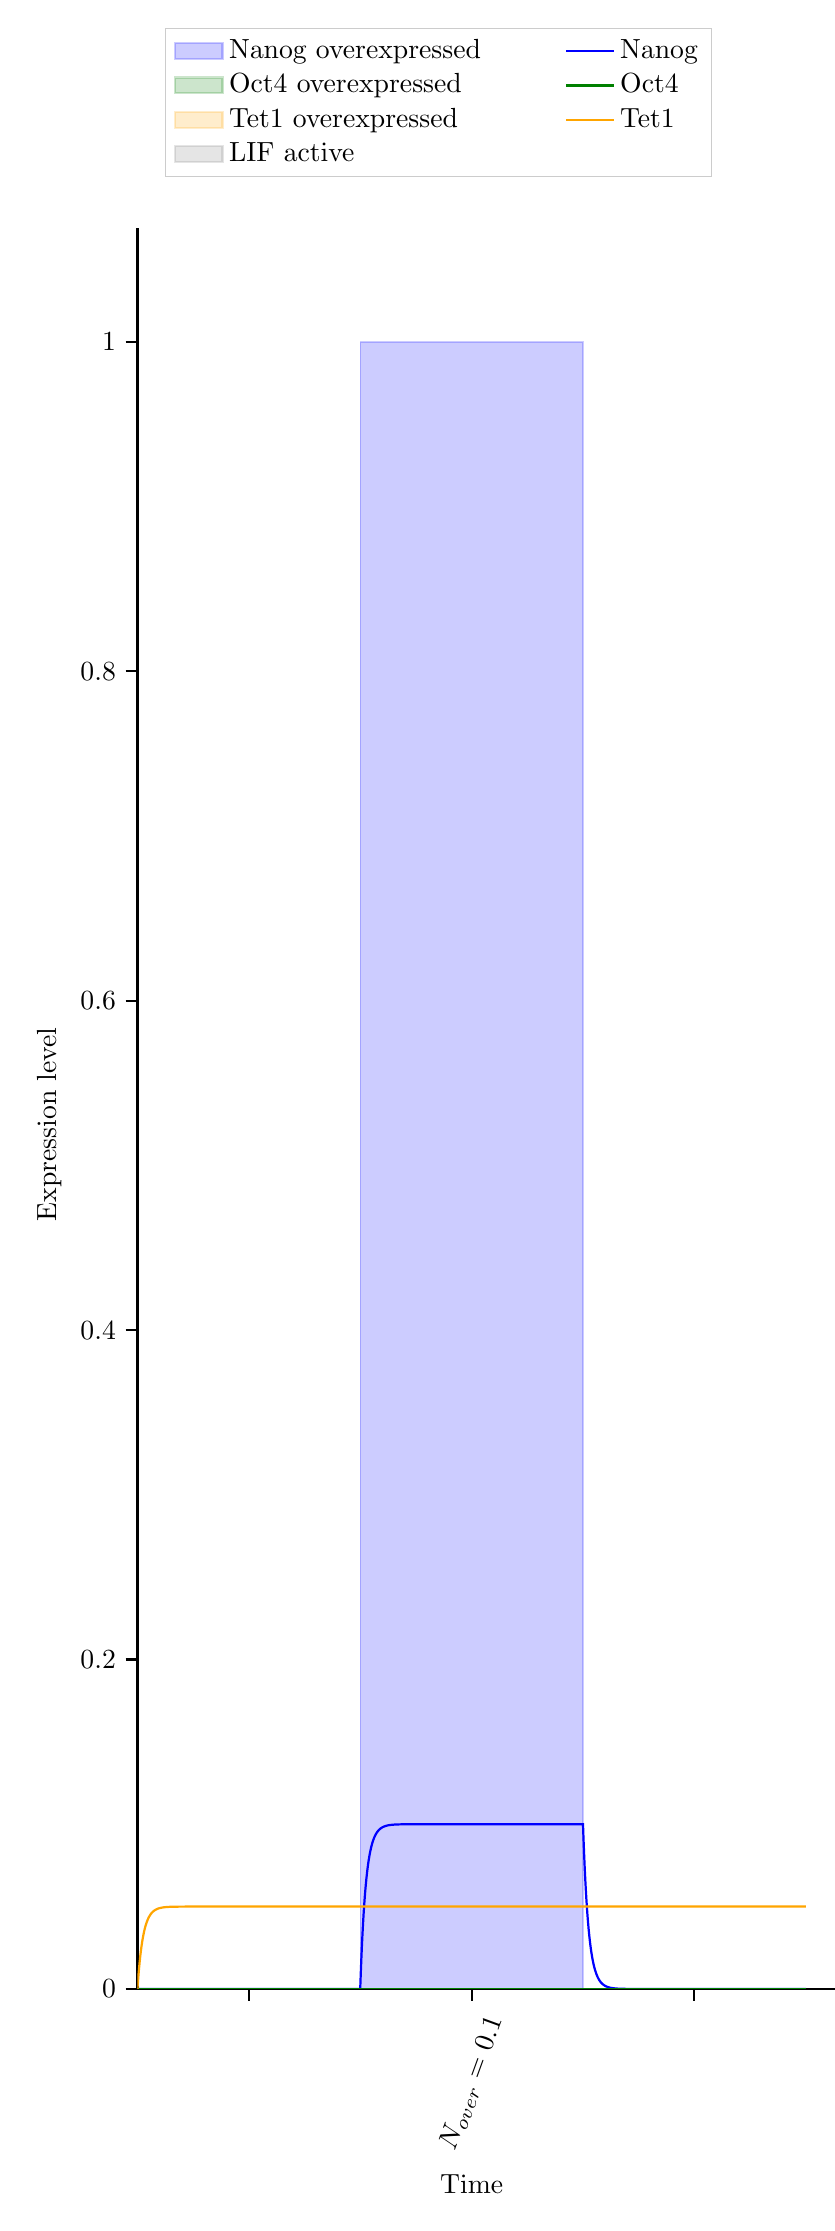
\begin{tikzpicture}[baseline]

\definecolor{darkgray176}{RGB}{176,176,176}
\definecolor{green}{RGB}{0,128,0}
\definecolor{lightgray204}{RGB}{204,204,204}
\definecolor{orange}{RGB}{255,165,0}

\begin{axis}[
 ytick={0,0.2,0.4,0.6,0.8,1},
 x tick label style = {rotate=70},
 y post scale=3, 
 transpose legend,
legend cell align={left},
legend style={fill opacity=0.8, draw opacity=1, text opacity=1, draw=lightgray204, anchor=south west,
    legend columns=4,
    /tikz/every even column/.append style={column sep=1.0cm},, at={(axis cs:5,1.1)}},
tick align=outside,
tick pos=left,
x grid style={darkgray176},
xlabel={Time},
xmin=0, xmax=120,
xtick style={color=black},
xtick={20,60,100},
xticklabels={,\(\displaystyle N_\text{over}=0.1\),},
y grid style={darkgray176},
ylabel={Expression level},
ymin=0, ymax=1.05,
ytick style={color=black}
]
\path [draw=blue, fill=blue, opacity=0.2]
(axis cs:40,0)
--(axis cs:40,1)
--(axis cs:80,1)
--(axis cs:80,0)
--cycle;
\addlegendimage{area legend, draw=blue, fill=blue, opacity=0.2}
\addlegendentry{Nanog overexpressed}
\addlegendimage{area legend, draw=green, fill=green, opacity=0.2}
\addlegendentry{Oct4 overexpressed}

\addlegendimage{area legend, draw=orange, fill=orange, opacity=0.2}
\addlegendentry{Tet1 overexpressed}

\addlegendimage{area legend, draw=gray, fill=gray, opacity=0.2}
\addlegendentry{LIF active}

\addplot [thick, blue]
table {%
0 0
0.0001 0
0.0011 0
0.0111 0
0.1111 0
0.2111 0
0.3111 0
0.4111 0
0.5111 0
0.6111 0
0.7111 0
0.8111 0
0.9111 0
1.0111 0
1.1111 0
1.2111 0
1.3111 0
1.4111 0
1.5111 0
1.6111 0
1.7111 0
1.8111 0
1.9111 0
2.0111 0
2.1111 0
2.2111 0
2.3111 0
2.4111 0
2.5111 0
2.6111 0
2.7111 0
2.8111 0
2.9111 0
3.0111 0
3.1111 0
3.2111 0
3.3111 0
3.4111 0
3.5111 0
3.6111 0
3.7111 0
3.8111 0
3.9111 0
4.0111 0
4.1111 0
4.2111 0
4.3111 0
4.4111 0
4.5111 0
4.6111 0
4.7111 0
4.8111 0
4.9111 0
5.0111 0
5.1111 0
5.2111 0
5.3111 0
5.4111 0
5.5111 0
5.6111 0
5.7111 0
5.8111 0
5.9111 0
6.0111 0
6.1111 0
6.21109999999999 0
6.31109999999999 0
6.41109999999999 0
6.51109999999999 0
6.61109999999999 0
6.71109999999999 0
6.81109999999999 0
6.91109999999999 0
7.01109999999999 0
7.11109999999999 0
7.21109999999999 0
7.31109999999999 0
7.41109999999999 0
7.51109999999999 0
7.61109999999999 0
7.71109999999999 0
7.81109999999999 0
7.91109999999999 0
8.01109999999999 0
8.11109999999999 0
8.21109999999999 0
8.31109999999999 0
8.41109999999999 0
8.51109999999999 0
8.61109999999999 0
8.71109999999999 0
8.81109999999999 0
8.91109999999999 0
9.01109999999998 0
9.11109999999998 0
9.21109999999998 0
9.31109999999998 0
9.41109999999998 0
9.51109999999998 0
9.61109999999998 0
9.71109999999998 0
9.81109999999998 0
9.91109999999998 0
10.0111 0
10.1111 0
10.2111 0
10.3111 0
10.4111 0
10.5111 0
10.6111 0
10.7111 0
10.8111 0
10.9111 0
11.0111 0
11.1111 0
11.2111 0
11.3111 0
11.4111 0
11.5111 0
11.6111 0
11.7111 0
11.8111 0
11.9111 0
12.0111 0
12.1111 0
12.2111 0
12.3111 0
12.4111 0
12.5111 0
12.6111 0
12.7111 0
12.8111 0
12.9111 0
13.0111 0
13.1111 0
13.2111 0
13.3111 0
13.4111 0
13.5111 0
13.6111 0
13.7111 0
13.8111 0
13.9111 0
14.0111 0
14.1111 0
14.2111 0
14.3111 0
14.4111 0
14.5111 0
14.6111 0
14.7111 0
14.8111 0
14.9111 0
15.0111 0
15.1111 0
15.2111 0
15.3111 0
15.4111 0
15.5111 0
15.6111 0
15.7111 0
15.8111 0
15.9111 0
16.0111 0
16.1111 0
16.2111 0
16.3111 0
16.4111 0
16.5111 0
16.6111 0
16.7111 0
16.8111 0
16.9111 0
17.0111 0
17.1111 0
17.2111 0
17.3111 0
17.4111 0
17.5111 0
17.6111 0
17.7111 0
17.8111 0
17.9111 0
18.0111 0
18.1111 0
18.2111 0
18.3111 0
18.4111 0
18.5111 0
18.6111 0
18.7111 0
18.8111 0
18.9111 0
19.0111 0
19.1111 0
19.2111 0
19.3111 0
19.4111 0
19.5111 0
19.6111 0
19.7111 0
19.8111 0
19.9111 0
20.0111 0
20.1111 0
20.2111 0
20.3111 0
20.4111 0
20.5111 0
20.6111 0
20.7111 0
20.8111 0
20.9111 0
21.0111 0
21.1111 0
21.2111 0
21.3111 0
21.4111 0
21.5111 0
21.6111 0
21.7111 0
21.8111 0
21.9111 0
22.0111 0
22.1111 0
22.2111 0
22.3111 0
22.4111000000001 0
22.5111000000001 0
22.6111000000001 0
22.7111000000001 0
22.8111000000001 0
22.9111000000001 0
23.0111000000001 0
23.1111000000001 0
23.2111000000001 0
23.3111000000001 0
23.4111000000001 0
23.5111000000001 0
23.6111000000001 0
23.7111000000001 0
23.8111000000001 0
23.9111000000001 0
24.0111000000001 0
24.1111000000001 0
24.2111000000001 0
24.3111000000001 0
24.4111000000001 0
24.5111000000001 0
24.6111000000001 0
24.7111000000001 0
24.8111000000001 0
24.9111000000001 0
25.0111000000001 0
25.1111000000001 0
25.2111000000001 0
25.3111000000001 0
25.4111000000001 0
25.5111000000001 0
25.6111000000001 0
25.7111000000001 0
25.8111000000001 0
25.9111000000001 0
26.0111000000001 0
26.1111000000001 0
26.2111000000001 0
26.3111000000001 0
26.4111000000001 0
26.5111000000001 0
26.6111000000001 0
26.7111000000001 0
26.8111000000001 0
26.9111000000001 0
27.0111000000001 0
27.1111000000001 0
27.2111000000001 0
27.3111000000001 0
27.4111000000001 0
27.5111000000001 0
27.6111000000001 0
27.7111000000001 0
27.8111000000001 0
27.9111000000001 0
28.0111000000001 0
28.1111000000001 0
28.2111000000001 0
28.3111000000001 0
28.4111000000001 0
28.5111000000001 0
28.6111000000001 0
28.7111000000001 0
28.8111000000001 0
28.9111000000001 0
29.0111000000001 0
29.1111000000001 0
29.2111000000001 0
29.3111000000001 0
29.4111000000002 0
29.5111000000002 0
29.6111000000002 0
29.7111000000002 0
29.8111000000002 0
29.9111000000002 0
30.0111000000002 0
30.1111000000002 0
30.2111000000002 0
30.3111000000002 0
30.4111000000002 0
30.5111000000002 0
30.6111000000002 0
30.7111000000002 0
30.8111000000002 0
30.9111000000002 0
31.0111000000002 0
31.1111000000002 0
31.2111000000002 0
31.3111000000002 0
31.4111000000002 0
31.5111000000002 0
31.6111000000002 0
31.7111000000002 0
31.8111000000002 0
31.9111000000002 0
32.0111000000002 0
32.1111000000002 0
32.2111000000002 0
32.3111000000002 0
32.4111000000002 0
32.5111000000002 0
32.6111000000002 0
32.7111000000002 0
32.8111000000002 0
32.9111000000002 0
33.0111000000002 0
33.1111000000002 0
33.2111000000002 0
33.3111000000002 0
33.4111000000002 0
33.5111000000002 0
33.6111000000002 0
33.7111000000002 0
33.8111000000002 0
33.9111000000002 0
34.0111000000002 0
34.1111000000002 0
34.2111000000002 0
34.3111000000002 0
34.4111000000002 0
34.5111000000002 0
34.6111000000002 0
34.7111000000002 0
34.8111000000002 0
34.9111000000002 0
35.0111000000002 0
35.1111000000002 0
35.2111000000002 0
35.3111000000002 0
35.4111000000002 0
35.5111000000002 0
35.6111000000002 0
35.7111000000002 0
35.8111000000002 0
35.9111000000002 0
36.0111000000002 0
36.1111000000002 0
36.2111000000002 0
36.3111000000002 0
36.4111000000002 0
36.5111000000002 0
36.6111000000002 0
36.7111000000003 0
36.8111000000003 0
36.9111000000003 0
37.0111000000003 0
37.1111000000003 0
37.2111000000003 0
37.3111000000003 0
37.4111000000003 0
37.5111000000003 0
37.6111000000003 0
37.7111000000003 0
37.8111000000003 0
37.9111000000003 0
38.0111000000003 0
38.1111000000003 0
38.2111000000003 0
38.3111000000003 0
38.4111000000003 0
38.5111000000003 0
38.6111000000003 0
38.7111000000003 0
38.8111000000003 0
38.9111000000003 0
39.0111000000003 0
39.1111000000003 0
39.2111000000003 0
39.3111000000003 0
39.4111000000003 0
39.5111000000003 0
39.6111000000003 0
39.7111000000003 0
39.8111000000003 0
39.9111000000003 0
40 0
40 0
40.0098039215686 0.000975601979910388
40.1078431372549 0.0102231587935491
40.2078431372549 0.0187665547766335
40.3078431372549 0.0264969391417669
40.4078431372549 0.0334916801734386
40.5078431372549 0.0398207835904466
40.6078431372549 0.0455475931866568
40.7078431372549 0.0507294247969782
40.8078431372549 0.0554181399334995
40.9078431372549 0.0596606648329298
41.0078431372549 0.0634994601101452
41.1078431372549 0.066972945718291
41.2078431372549 0.0701158854685836
41.3078431372549 0.0729597349582156
41.4078431372549 0.0755329563885427
41.5078431372549 0.07786130342436
41.6078431372549 0.0799680789452329
41.7078431372549 0.0818743682685474
41.8078431372549 0.0835992501784517
41.9078431372549 0.0851599878727394
42.0078431372549 0.0865722017387342
42.1078431372549 0.0878500256873754
42.2078431372549 0.0890062486101485
42.3078431372549 0.0900524423746083
42.4078431372549 0.0909990776395185
42.5078431372549 0.0918556286487232
42.6078431372549 0.0926306680525627
42.7078431372549 0.0933319527058395
42.8078431372549 0.0939665013010273
42.9078431372549 0.094540664613704
43.0078431372549 0.0950601890632481
43.1078431372549 0.0955302742249347
43.2078431372549 0.0959556248690319
43.3078431372549 0.0963404980477233
43.4078431372549 0.0966887457011162
43.5078431372549 0.0970038532087528
43.6078431372549 0.0972889742724602
43.7078431372549 0.0975469624796576
43.8078431372549 0.0977803998630186
43.9078431372549 0.0979916227423215
44.0078431372549 0.0981827451071228
44.1078431372549 0.0983556797742754
44.2078431372549 0.098512157532042
44.3078431372549 0.0986537444624062
44.4078431372549 0.0987818576149467
44.5078431372549 0.098897779189146
44.6078431372549 0.0990026693670736
44.7078431372549 0.0990975779248781
44.8078431372549 0.0991834547392997
44.907843137255 0.0992611592943556
45.007843137255 0.0993314692833452
45.107843137255 0.0993950883922655
45.207843137255 0.0994526533425377
45.307843137255 0.0995047402635284
45.407843137255 0.0995518704586466
45.507843137255 0.0995945156227229
45.607843137255 0.0996331025628901
45.707843137255 0.0996680174702123
45.807843137255 0.0996996097848152
45.907843137255 0.0997281956931995
46.007843137255 0.0997540612927428
46.107843137255 0.0997774654550572
46.207843137255 0.0997986424168639
46.307843137255 0.0998178041243133
46.407843137255 0.0998351423542127
46.507843137255 0.0998508306333933
46.607843137255 0.0998650259754252
46.707843137255 0.0998778704520617
46.807843137255 0.0998894926151413
46.907843137255 0.0999000087831776
47.007843137255 0.0999095242055145
47.107843137255 0.099918134115696
47.207843137255 0.0999259246845968
47.307843137255 0.0999329738828484
47.407843137255 0.0999393522611956
47.507843137255 0.0999451236565925
47.607843137255 0.0999503458311036
47.707843137255 0.0999550710500063
47.807843137255 0.0999593466048792
47.907843137255 0.0999632152869125
48.007843137255 0.0999667158151757
48.107843137255 0.0999698832241323
48.207843137255 0.0999727492142753
48.307843137255 0.0999753424693973
48.407843137255 0.099977688943667
48.507843137255 0.0999798121213874
48.607843137255 0.0999817332520345
48.707843137255 0.0999834715629296
48.807843137255 0.0999850444516721
48.907843137255 0.0999864676602612
49.007843137255 0.0999877554326468
49.107843137255 0.0999889206572875
49.207843137255 0.0999899749961432
49.307843137255 0.0999909290013914
49.407843137255 0.0999917922210373
49.507843137255 0.0999925732944731
49.607843137255 0.0999932800389444
49.707843137255 0.0999939195277871
49.807843137255 0.0999944981612206
49.907843137255 0.0999950217304028
50.007843137255 0.0999954954753899
50.107843137255 0.099995924137581
50.207843137255 0.0999963120071713
50.307843137255 0.09999666296609
50.407843137255 0.099996980526852
50.507843137255 0.099997267867712
50.607843137255 0.099997527864474
50.707843137255 0.0999977631192729
50.807843137255 0.0999979759866178
50.907843137255 0.0999981685969566
51.007843137255 0.0999983428779982
51.107843137255 0.0999985005740061
51.207843137255 0.0999986432632547
51.307843137255 0.099998772373826
51.407843137255 0.099998889197902
51.507843137255 0.0999989949046974
51.607843137255 0.0999990905521612
51.707843137255 0.0999991770975654
51.807843137255 0.0999992554070856
51.907843137255 0.0999993262644696
52.0078431372551 0.099999390378882
52.1078431372551 0.0999994483920014
52.2078431372551 0.0999995008844427
52.3078431372551 0.0999995483815676
52.4078431372551 0.0999995913587436
52.5078431372551 0.0999996302461005
52.6078431372551 0.0999996654328362
52.7078431372551 0.0999996972711112
52.8078431372551 0.0999997260795738
52.9078431372551 0.0999997521465488
53.0078431372551 0.0999997757329231
53.1078431372551 0.0999997970747571
53.2078431372551 0.0999998163856471
53.3078431372551 0.0999998338588629
53.4078431372551 0.0999998496692825
53.5078431372551 0.0999998639751417
53.6078431372551 0.0999998769196183
53.7078431372551 0.0999998886322652
53.8078431372551 0.0999998992303064
53.9078431372551 0.0999999088198106
54.0078431372551 0.0999999174967528
54.1078431372551 0.0999999253479748
54.2078431372551 0.0999999324520542
54.3078431372551 0.0999999388800911
54.4078431372551 0.0999999446964195
54.5078431372551 0.099999949959251
54.6078431372551 0.0999999547212578
54.7078431372551 0.0999999590300998
54.8078431372551 0.0999999629289013
54.9078431372551 0.0999999664566828
55.0078431372551 0.0999999696487514
55.1078431372551 0.0999999725370546
55.2078431372551 0.0999999751504994
55.3078431372551 0.099999977515242
55.4078431372551 0.0999999796549496
55.5078431372551 0.0999999815910372
55.6078431372551 0.0999999833428816
55.7078431372551 0.099999984928016
55.8078431372551 0.0999999863623049
55.9078431372551 0.0999999876601032
56.0078431372551 0.0999999888343996
56.1078431372551 0.0999999898969469
56.2078431372551 0.0999999908583796
56.3078431372551 0.0999999917283198
56.4078431372551 0.0999999925154742
56.5078431372551 0.099999993227721
56.6078431372551 0.0999999938721886
56.7078431372551 0.0999999944553269
56.8078431372551 0.0999999949829723
56.9078431372551 0.0999999954604056
57.0078431372551 0.0999999958924051
57.1078431372551 0.0999999962832945
57.2078431372551 0.0999999966369858
57.3078431372551 0.0999999969570189
57.4078431372551 0.0999999972465968
57.5078431372551 0.0999999975086178
57.6078431372551 0.0999999977457042
57.7078431372551 0.0999999979602288
57.8078431372551 0.0999999981543387
57.9078431372551 0.0999999983299766
58.0078431372551 0.0999999984889003
58.1078431372551 0.0999999986327005
58.2078431372551 0.0999999987628162
58.3078431372551 0.0999999988805498
58.4078431372551 0.0999999989870796
58.5078431372551 0.0999999990834717
58.6078431372551 0.0999999991706909
58.7078431372551 0.0999999992496101
58.8078431372551 0.0999999993210191
58.9078431372551 0.0999999993856327
59.0078431372552 0.0999999994440975
59.1078431372552 0.0999999994969986
59.2078431372552 0.0999999995448655
59.3078431372552 0.0999999995881773
59.4078431372552 0.0999999996273674
59.5078431372552 0.0999999996628281
59.6078431372552 0.0999999996949142
59.7078431372552 0.099999999723947
59.8078431372552 0.0999999997502169
59.9078431372552 0.0999999997739869
60.0078431372552 0.0999999997954949
60.1078431372552 0.0999999998149561
60.2078431372552 0.0999999998325654
60.3078431372552 0.0999999998484989
60.4078431372552 0.0999999998629161
60.5078431372552 0.0999999998759614
60.6078431372552 0.0999999998877652
60.7078431372552 0.0999999998984458
60.8078431372552 0.0999999999081099
60.9078431372552 0.0999999999168544
61.0078431372552 0.0999999999247668
61.1078431372552 0.0999999999319262
61.2078431372552 0.0999999999384042
61.3078431372552 0.0999999999442659
61.4078431372552 0.0999999999495697
61.5078431372552 0.0999999999543687
61.6078431372552 0.0999999999587111
61.7078431372552 0.0999999999626403
61.8078431372552 0.0999999999661955
61.9078431372552 0.0999999999694125
62.0078431372552 0.0999999999723233
62.1078431372552 0.0999999999749571
62.2078431372552 0.0999999999773402
62.3078431372552 0.0999999999794966
62.4078431372552 0.0999999999814477
62.5078431372552 0.0999999999832132
62.6078431372552 0.0999999999848107
62.7078431372552 0.0999999999862561
62.8078431372552 0.099999999987564
62.9078431372552 0.0999999999887475
63.0078431372552 0.0999999999898183
63.1078431372552 0.0999999999907872
63.2078431372552 0.0999999999916639
63.3078431372552 0.0999999999924572
63.4078431372552 0.099999999993175
63.5078431372552 0.0999999999938245
63.6078431372552 0.0999999999944122
63.7078431372552 0.0999999999949439
63.8078431372552 0.0999999999954251
63.9078431372552 0.0999999999958604
64.0078431372552 0.0999999999962544
64.1078431372552 0.0999999999966108
64.2078431372552 0.0999999999969333
64.3078431372552 0.0999999999972252
64.4078431372552 0.0999999999974892
64.5078431372552 0.0999999999977282
64.6078431372552 0.0999999999979444
64.7078431372552 0.09999999999814
64.8078431372552 0.099999999998317
64.9078431372552 0.0999999999984772
65.0078431372552 0.0999999999986221
65.1078431372552 0.0999999999987532
65.2078431372552 0.0999999999988719
65.3078431372551 0.0999999999989792
65.4078431372551 0.0999999999990764
65.5078431372551 0.0999999999991643
65.6078431372551 0.0999999999992438
65.7078431372551 0.0999999999993157
65.8078431372551 0.0999999999993809
65.9078431372551 0.0999999999994398
66.0078431372551 0.0999999999994931
66.1078431372551 0.0999999999995413
66.2078431372551 0.099999999999585
66.3078431372551 0.0999999999996245
66.4078431372551 0.0999999999996602
66.5078431372551 0.0999999999996926
66.6078431372551 0.0999999999997218
66.7078431372551 0.0999999999997483
66.8078431372551 0.0999999999997722
66.9078431372551 0.0999999999997939
67.0078431372551 0.0999999999998135
67.107843137255 0.0999999999998313
67.207843137255 0.0999999999998473
67.307843137255 0.0999999999998619
67.407843137255 0.099999999999875
67.507843137255 0.0999999999998869
67.607843137255 0.0999999999998977
67.707843137255 0.0999999999999074
67.807843137255 0.0999999999999162
67.907843137255 0.0999999999999242
68.007843137255 0.0999999999999314
68.107843137255 0.0999999999999379
68.207843137255 0.0999999999999439
68.307843137255 0.0999999999999492
68.407843137255 0.099999999999954
68.507843137255 0.0999999999999584
68.607843137255 0.0999999999999624
68.707843137255 0.0999999999999659
68.8078431372549 0.0999999999999692
68.9078431372549 0.0999999999999721
69.0078431372549 0.0999999999999748
69.1078431372549 0.0999999999999772
69.2078431372549 0.0999999999999793
69.3078431372549 0.0999999999999813
69.4078431372549 0.0999999999999831
69.5078431372549 0.0999999999999847
69.6078431372549 0.0999999999999862
69.7078431372549 0.0999999999999875
69.8078431372549 0.0999999999999887
69.9078431372549 0.0999999999999897
70.0078431372549 0.0999999999999907
70.1078431372549 0.0999999999999916
70.2078431372549 0.0999999999999924
70.3078431372549 0.0999999999999931
70.4078431372549 0.0999999999999938
70.5078431372549 0.0999999999999944
70.6078431372548 0.0999999999999949
70.7078431372548 0.0999999999999954
70.8078431372548 0.0999999999999958
70.9078431372548 0.0999999999999962
71.0078431372548 0.0999999999999966
71.1078431372548 0.0999999999999969
71.2078431372548 0.0999999999999972
71.3078431372548 0.0999999999999975
71.4078431372548 0.0999999999999977
71.5078431372548 0.0999999999999979
71.6078431372548 0.0999999999999981
71.7078431372548 0.0999999999999983
71.8078431372548 0.0999999999999985
71.9078431372548 0.0999999999999986
72.0078431372548 0.0999999999999987
72.1078431372548 0.0999999999999989
72.2078431372548 0.099999999999999
72.3078431372547 0.0999999999999991
72.4078431372547 0.0999999999999992
72.5078431372547 0.0999999999999992
72.6078431372547 0.0999999999999993
72.7078431372547 0.0999999999999994
72.8078431372547 0.0999999999999994
72.9078431372547 0.0999999999999995
73.0078431372547 0.0999999999999995
73.1078431372547 0.0999999999999996
73.2078431372547 0.0999999999999996
73.3078431372547 0.0999999999999997
73.4078431372547 0.0999999999999997
73.5078431372547 0.0999999999999997
73.6078431372547 0.0999999999999998
73.7078431372547 0.0999999999999998
73.8078431372547 0.0999999999999998
73.9078431372547 0.0999999999999998
74.0078431372547 0.0999999999999998
74.1078431372546 0.0999999999999999
74.2078431372546 0.0999999999999999
74.3078431372546 0.0999999999999999
74.4078431372546 0.0999999999999999
74.5078431372546 0.0999999999999999
74.6078431372546 0.0999999999999999
74.7078431372546 0.0999999999999999
74.8078431372546 0.0999999999999999
74.9078431372546 0.0999999999999999
75.0078431372546 0.0999999999999999
75.1078431372546 0.0999999999999999
75.2078431372546 0.0999999999999999
75.3078431372546 0.0999999999999999
75.4078431372546 0.0999999999999999
75.5078431372546 0.0999999999999999
75.6078431372546 0.0999999999999999
75.7078431372546 0.0999999999999999
75.8078431372546 0.0999999999999999
75.9078431372545 0.0999999999999999
76.0078431372545 0.0999999999999999
76.1078431372545 0.0999999999999999
76.2078431372545 0.0999999999999999
76.3078431372545 0.0999999999999999
76.4078431372545 0.0999999999999999
76.5078431372545 0.0999999999999999
76.6078431372545 0.0999999999999999
76.7078431372545 0.0999999999999999
76.8078431372545 0.0999999999999999
76.9078431372545 0.0999999999999999
77.0078431372545 0.0999999999999999
77.1078431372545 0.0999999999999999
77.2078431372545 0.0999999999999999
77.3078431372545 0.0999999999999999
77.4078431372545 0.0999999999999999
77.5078431372545 0.0999999999999999
77.6078431372544 0.0999999999999999
77.7078431372544 0.0999999999999999
77.8078431372544 0.0999999999999999
77.9078431372544 0.0999999999999999
78.0078431372544 0.0999999999999999
78.1078431372544 0.0999999999999999
78.2078431372544 0.0999999999999999
78.3078431372544 0.0999999999999999
78.4078431372544 0.0999999999999999
78.5078431372544 0.0999999999999999
78.6078431372544 0.0999999999999999
78.7078431372544 0.0999999999999999
78.8078431372544 0.0999999999999999
78.9078431372544 0.0999999999999999
79.0078431372544 0.0999999999999999
79.1078431372544 0.0999999999999999
79.2078431372544 0.0999999999999999
79.3078431372544 0.0999999999999999
79.4078431372543 0.0999999999999999
79.5078431372543 0.0999999999999999
79.6078431372543 0.0999999999999999
79.7078431372543 0.0999999999999999
79.8078431372543 0.0999999999999999
79.9078431372543 0.0999999999999999
80 0.0999999999999999
80 0.0999999999999999
80.1 0.0904837418333338
80.2 0.081873075361614
80.3 0.0740818221412137
80.4 0.0670320046916854
80.5 0.0606530660709328
80.6 0.0548811637176243
80.7 0.0496585304933844
80.8 0.0449328965298613
80.8999999999999 0.0406569660943187
80.9999999999999 0.0367879442380495
81.0999999999999 0.0332871084901475
81.1999999999999 0.0301194213100068
81.2999999999999 0.0272531794198407
81.3999999999999 0.0246596965076239
81.4999999999999 0.0223130161248421
81.5999999999999 0.0201896519056323
81.6999999999999 0.0182683525073411
81.7999999999999 0.0165298889199459
81.8999999999999 0.0149568620156607
81.9999999999999 0.0135335284126184
82.0999999999999 0.0122456429098145
82.1999999999999 0.0110803159163485
82.2999999999999 0.0100258844480666
82.3999999999999 0.00907179540049692
82.4999999999999 0.00820849992983389
82.5999999999999 0.00742735788490029
82.6999999999998 0.00672055133361094
82.7999999999998 0.0060810063184812
82.8999999999998 0.00550232205808325
82.9999999999998 0.00497870688587463
83.0999999999998 0.00450492028525321
83.1999999999998 0.004076220440706
83.2999999999998 0.003688316780126
83.3999999999998 0.00333732703332474
83.4999999999998 0.00301973837696762
83.5999999999998 0.00273237227705749
83.6999999999998 0.00247235267709828
83.7999999999998 0.00223707721355513
83.8999999999998 0.00202419117052556
83.9999999999998 0.00183156391295149
84.0999999999998 0.00165726756250753
84.1999999999998 0.0014995577027469
84.2999999999998 0.00135685592039538
84.3999999999997 0.00122773400806086
84.4999999999997 0.00111089967025383
84.5999999999997 0.00100518358965983
84.6999999999997 0.00090952772421884
84.7999999999997 0.000822974717884772
84.8999999999997 0.000744658319084464
84.9999999999997 0.00067379471098083
85.0999999999997 0.000609674666770552
85.1999999999997 0.000551656451503905
85.2999999999997 0.000499159399385724
85.3999999999997 0.000451658102276998
85.4999999999997 0.000408677151233654
85.5999999999997 0.000369786378454083
85.6999999999997 0.000334596552015227
85.7999999999997 0.000302755480308695
85.8999999999997 0.000273944487188789
85.9999999999997 0.000247875222554554
86.0999999999997 0.000224286776445065
86.1999999999996 0.000202943067764859
86.2999999999996 0.000183630481505003
86.3999999999996 0.000166155730812295
86.4999999999996 0.000150343922509486
86.5999999999996 0.000136036806705591
86.6999999999996 0.000123091192977798
86.7999999999996 0.000111377517273601
86.8999999999996 0.000100778545190222
86.9999999999996 9.11881986533105e-05
87.0999999999996 8.25104942519291e-05
87.1999999999996 7.46585826043233e-05
87.2999999999996 6.75538791401221e-05
87.3999999999996 6.11252775995505e-05
87.4999999999996 5.53084383780859e-05
87.5999999999996 5.00451445940758e-05
87.6999999999996 4.52827194346222e-05
87.7999999999996 4.09734989483364e-05
87.8999999999996 3.70743550084965e-05
87.9999999999995 3.35462636722616e-05
88.0999999999995 3.03539146159387e-05
88.1999999999995 2.74653577373965e-05
88.2999999999995 2.48516833887075e-05
88.3999999999995 2.24867330386756e-05
88.4999999999995 2.03468374694662e-05
88.5999999999995 1.84105798871198e-05
88.6999999999995 1.66585815750812e-05
88.7999999999995 1.50733079454918e-05
88.8999999999995 1.36388930471422e-05
88.9999999999995 1.23409807737007e-05
89.0999999999995 1.11665811829767e-05
89.1999999999995 1.01039404892142e-05
89.2999999999995 9.14242342725431e-06
89.3999999999995 8.27240681122702e-06
89.4999999999995 7.48518322247378e-06
89.5999999999995 6.7728738627752e-06
89.6999999999994 6.12834970069085e-06
89.7999999999994 5.545160121817e-06
89.8999999999994 5.01746836886987e-06
89.9999999999994 4.5399931254574e-06
90.0999999999994 4.10795565888998e-06
90.1999999999994 3.71703199301784e-06
90.2999999999994 3.36330963242469e-06
90.3999999999994 3.0432484048588e-06
90.4999999999994 2.75364502999949e-06
90.5999999999994 2.49160105995117e-06
90.6999999999994 2.25449387060282e-06
90.7999999999994 2.03995041352459e-06
90.8999999999994 1.84582346570162e-06
90.9999999999994 1.67017013940455e-06
91.0999999999994 1.51123243711624e-06
91.1999999999994 1.36741965690186e-06
91.2999999999994 1.23729247212934e-06
91.3999999999994 1.11954852620479e-06
91.4999999999993 1.01300939815003e-06
91.5999999999993 9.16608808569485e-07
91.6999999999993 8.2938194796761e-07
91.7999999999993 7.50455820611287e-07
91.8999999999993 6.79040507295144e-07
91.9999999999993 6.14421259564699e-07
92.0999999999993 5.5595134627364e-07
92.1999999999993 5.03045580881184e-07
92.2999999999993 4.55174464708525e-07
92.3999999999993 4.11858887538121e-07
92.4999999999993 3.72665332517635e-07
92.5999999999993 3.37201537377592e-07
92.6999999999993 3.05112568538773e-07
92.7999999999993 2.76077268817677e-07
92.8999999999993 2.49805043177506e-07
92.9999999999993 2.26032950355383e-07
93.0999999999993 2.04523071257832e-07
93.1999999999992 1.85060127786542e-07
93.2999999999992 1.67449328262812e-07
93.3999999999992 1.51514417886975e-07
93.4999999999992 1.37095914721129e-07
93.5999999999992 1.24049513540314e-07
93.6999999999992 1.12244641577324e-07
93.7999999999992 1.01563151706577e-07
93.8999999999992 9.18981399879762e-08
93.9999999999992 8.31528757363562e-08
94.0999999999992 7.52398334082774e-08
94.1999999999992 6.80798166169762e-08
94.2999999999992 6.16011655083119e-08
94.3999999999992 5.57390395648656e-08
94.4999999999992 5.04347686602528e-08
94.5999999999992 4.56352658687823e-08
94.6999999999992 4.12924961536645e-08
94.7999999999992 3.73629956162211e-08
94.8999999999992 3.38074364945813e-08
94.9999999999991 3.05902335582253e-08
95.0999999999991 2.76791879590384e-08
95.1999999999991 2.50451649744195e-08
95.2999999999991 2.26618024171863e-08
95.3999999999991 2.05052467939471e-08
95.4999999999991 1.85539145713231e-08
95.5999999999991 1.67882761606933e-08
95.6999999999991 1.51906604595088e-08
95.7999999999991 1.37450779929603e-08
95.8999999999991 1.24370608859406e-08
95.9999999999991 1.1253518063689e-08
96.0999999999991 1.0182604231916e-08
96.1999999999991 9.21360132511696e-09
96.2999999999991 8.33681123657145e-09
96.3999999999991 7.54345875643168e-09
96.4999999999991 6.82560374647366e-09
96.5999999999991 6.17606167252559e-09
96.6999999999991 5.58833169923553e-09
96.799999999999 5.05653162752664e-09
96.899999999999 4.57533902357208e-09
96.999999999999 4.13993795008874e-09
97.099999999999 3.74597076681851e-09
97.199999999999 3.38949451780021e-09
97.299999999999 3.06694146894135e-09
97.399999999999 2.77508340093635e-09
97.499999999999 2.51099930016294e-09
97.599999999999 2.27204612419626e-09
97.699999999999 2.05583234935201e-09
97.799999999999 1.86019403551384e-09
97.899999999999 1.68317316869341e-09
97.999999999999 1.52299806456849e-09
98.099999999999 1.37806563687083e-09
98.199999999999 1.24692535316009e-09
98.299999999999 1.12826471740776e-09
98.399999999999 1.02089613409583e-09
98.4999999999989 9.23745022361757e-10
98.5999999999989 8.35839061232084e-10
98.6999999999989 7.562984583074e-10
98.7999999999989 6.84327144504352e-10
98.8999999999989 6.19204806728743e-10
98.9999999999989 5.6027967874003e-10
99.0999999999989 5.06962018055761e-10
99.1999999999989 4.58718203610634e-10
99.2999999999989 4.15065395097553e-10
99.3999999999989 3.75566700539577e-10
99.4999999999989 3.39826803728201e-10
99.5999999999989 3.07488007765895e-10
99.6999999999989 2.78226655115354e-10
99.7999999999989 2.51749888326097e-10
99.8999999999989 2.27792719018692e-10
99.9999999999989 2.06115375792005e-10
100.099999999999 1.86500904510444e-10
100.199999999999 1.68752996954062e-10
100.299999999999 1.52694026099927e-10
100.399999999999 1.38163268371182e-10
100.499999999999 1.25015295061476e-10
100.599999999999 1.13118516835607e-10
100.699999999999 1.02353866739227e-10
100.799999999999 9.26136085367565e-11
100.899999999999 8.38002584509332e-11
100.999999999999 7.58256095124089e-11
101.099999999999 6.86098487547599e-11
101.199999999999 6.20807584194978e-11
101.299999999999 5.6172993176474e-11
101.399999999999 5.0827426125857e-11
101.499999999999 4.59905570362489e-11
101.599999999999 4.16139768963916e-11
101.699999999999 3.76538834215142e-11
101.799999999999 3.40706426653474e-11
101.899999999999 3.08283923502706e-11
101.999999999999 2.78946829455861e-11
102.099999999999 2.52401529017111e-11
102.199999999999 2.2838234789923e-11
102.299999999999 2.06648894066046e-11
102.399999999999 1.86983651808161e-11
102.499999999999 1.69189804772636e-11
102.599999999999 1.53089266158793e-11
102.699999999999 1.38520896365668e-11
102.799999999999 1.25338890252731e-11
102.899999999999 1.13411317873047e-11
102.999999999999 1.02618804074029e-11
103.099999999999 9.28533337507992e-12
103.199999999999 8.4017170794717e-12
103.299999999999 7.60218799175629e-12
103.399999999999 6.87874415614547e-12
103.499999999999 6.2241451036222e-12
103.599999999999 5.6318393868936e-12
103.699999999999 5.09589901130482e-12
103.799999999999 4.61096010547647e-12
103.899999999999 4.17216923787734e-12
103.999999999999 3.77513484205071e-12
104.099999999999 3.4158832643414e-12
104.199999999999 3.09081899423473e-12
104.299999999999 2.796688679279e-12
104.399999999999 2.53054856444088e-12
104.499999999999 2.28973503001582e-12
104.599999999999 2.07183793322693e-12
104.699999999999 1.87467648670613e-12
104.799999999999 1.69627743244139e-12
104.899999999999 1.53485529274737e-12
104.999999999999 1.38879450060479e-12
105.099999999999 1.25663323052278e-12
105.199999999999 1.13704876809811e-12
105.299999999999 1.028844271845e-12
105.399999999999 9.30936794803273e-13
105.499999999999 8.42346446041306e-13
105.599999999999 7.62186583578278e-13
105.699999999999 6.89654940573277e-13
105.799999999999 6.24025595969156e-13
105.899999999999 5.64641709230654e-13
105.999999999999 5.10908946463588e-13
106.099999999999 4.62289532121519e-13
106.199999999999 4.18296866767362e-13
106.299999999999 3.78490657022705e-13
106.399999999998 3.42472508963713e-13
106.499999999998 3.09881940860867e-13
106.599999999998 2.80392775356671e-13
106.699999999998 2.5370987497305e-13
106.799999999998 2.29566188276289e-13
106.899999999998 2.07720077136542e-13
106.999999999998 1.87952898332231e-13
107.099999999998 1.70066815295204e-13
107.199999999998 1.53882818095885e-13
107.299999999998 1.3923893185174e-13
107.399999999998 1.2598859562822e-13
107.499999999998 1.13999195607681e-13
107.599999999998 1.03150737845732e-13
107.699999999998 9.33346473315108e-14
107.799999999998 8.44526813324968e-14
107.899999999998 7.64159461482245e-14
107.999999999998 6.91440074322589e-14
108.099999999998 6.25640851782263e-14
108.199999999998 5.66103253130534e-14
108.299999999998 5.12231406072737e-14
108.399999999998 4.63486143060111e-14
108.499999999998 4.19379605119787e-14
108.599999999998 3.79470359198243e-14
108.699999999998 3.43358980150963e-14
108.799999999998 3.10684053161365e-14
108.899999999998 2.81118556579868e-14
108.999999999998 2.54366588981322e-14
109.099999999998 2.30160407684117e-14
109.199999999998 2.08257749091445e-14
109.299999999998 1.88439404035815e-14
109.399999999998 1.7050702386004e-14
109.499999999998 1.54281135277219e-14
109.599999999998 1.39599344141776e-14
109.699999999998 1.26314710154272e-14
109.799999999998 1.14294276233515e-14
109.899999999998 1.03417737837411e-14
109.999999999998 9.35762389146772e-15
110.099999999998 8.46712824369002e-15
110.199999999998 7.66137446071777e-15
110.299999999998 6.93229828792084e-15
110.399999999998 6.27260288595892e-15
110.499999999998 5.67568580156131e-15
110.599999999998 5.13557288795593e-15
110.699999999998 4.64685851360073e-15
110.799999999998 4.20465146080678e-15
110.899999999998 3.8045259727879e-15
110.999999999998 3.44247745919954e-15
111.099999999998 3.11488241685282e-15
111.199999999998 2.81846216447702e-15
111.299999999998 2.55025002857558e-15
111.399999999998 2.30756165196085e-15
111.499999999998 2.08796812780527e-15
111.599999999998 1.88927169032561e-15
111.699999999998 1.70948371880449e-15
111.799999999998 1.54680483480593e-15
111.899999999998 1.39960689339132e-15
111.999999999998 1.26641668809775e-15
112.099999999998 1.14590120659262e-15
112.199999999998 1.03685428943833e-15
112.299999999998 9.38184558443224e-16
112.399999999998 8.4890449378197e-16
112.499999999998 7.68120550565247e-16
112.599999999998 6.95024215942241e-16
112.699999999998 6.2888391723233e-16
112.799999999998 5.69037700099859e-16
112.899999999998 5.14886603492697e-16
112.999999999998 4.65888665038753e-16
113.099999999998 4.21553496904431e-16
113.199999999998 3.81437377828396e-16
113.299999999998 3.45138812210084e-16
113.399999999998 3.12294511806807e-16
113.499999999998 2.82575759822942e-16
113.599999999998 2.55685121001772e-16
113.699999999998 2.31353464793491e-16
113.799999999998 2.09337271806215e-16
113.899999999998 1.8941619658208e-16
113.999999999998 1.71390862305849e-16
114.099999999998 1.55080865374749e-16
114.199999999998 1.40322969858588e-16
114.299999999998 1.26969473779712e-16
114.399999999998 1.14886730861977e-16
114.499999999998 1.03953812953908e-16
114.599999999998 9.40612997391213e-17
114.699999999998 8.51101836210248e-17
114.799999999998 7.70108788215245e-17
114.899999999998 6.96823247764498e-17
114.999999999998 6.30511748541881e-17
115.099999999998 5.70510622779474e-17
115.199999999998 5.16219359047525e-17
115.299999999998 4.67094592134253e-17
115.399999999998 4.22644664864221e-17
115.499999999998 3.82424707428101e-17
115.599999999998 3.46032184976125e-17
115.699999999998 3.13102868914041e-17
115.799999999998 2.83307191580943e-17
115.899999999998 2.56346947825369e-17
115.999999999998 2.31952310467938e-17
116.099999999998 2.09879129780262e-17
116.199999999998 1.8990648995242e-17
116.299999999998 1.71834498093294e-17
116.399999999998 1.55482283635341e-17
116.499999999998 1.40686188121174e-17
116.599999999998 1.27298127254721e-17
116.699999999998 1.15184108823831e-17
116.799999999998 1.04222891661181e-17
116.899999999998 9.43047722219385e-18
116.999999999998 8.53304866338123e-18
117.099999999998 7.72102172308662e-18
117.199999999998 6.98626936281332e-18
117.299999999998 6.3214379340293e-18
117.399999999998 5.71987358038151e-18
117.499999999998 5.17555564366547e-18
117.599999999998 4.68303640705481e-18
117.699999999998 4.2373865725205e-18
117.799999999998 3.83414592675981e-18
117.899999999998 3.46927870188263e-18
117.999999999998 3.13913318409031e-18
118.099999999998 2.84040516609679e-18
118.199999999998 2.5701048775117e-18
118.299999999998 2.32552706221361e-18
118.399999999998 2.10422390323767e-18
118.499999999998 1.90398052420088e-18
118.599999999998 1.72279282207488e-18
118.699999999998 1.55884740944944e-18
118.799999999998 1.41050346554184e-18
118.899999999998 1.27627631431111e-18
118.999999999998 1.15482256532125e-18
119.099999999998 1.04492666863836e-18
119.199999999998 9.45488749198394e-19
119.299999999998 8.55513598887892e-19
119.399999999998 7.74100716166783e-19
119.499999999998 7.00435293546341e-19
119.599999999998 6.33780062722025e-19
119.699999999998 5.73467915744538e-19
119.799999999998 5.18895228379289e-19
119.899999999998 4.69515818832204e-19
119.999999999998 4.24835481378795e-19
120 4.24835481377829e-19
};
\addlegendentry{Nanog}
\addplot [thick, green]
table {%
0 0
0.0001 0
0.0011 0
0.0111 0
0.1111 0
0.2111 0
0.3111 0
0.4111 0
0.5111 0
0.6111 0
0.7111 0
0.8111 0
0.9111 0
1.0111 0
1.1111 0
1.2111 0
1.3111 0
1.4111 0
1.5111 0
1.6111 0
1.7111 0
1.8111 0
1.9111 0
2.0111 0
2.1111 0
2.2111 0
2.3111 0
2.4111 0
2.5111 0
2.6111 0
2.7111 0
2.8111 0
2.9111 0
3.0111 0
3.1111 0
3.2111 0
3.3111 0
3.4111 0
3.5111 0
3.6111 0
3.7111 0
3.8111 0
3.9111 0
4.0111 0
4.1111 0
4.2111 0
4.3111 0
4.4111 0
4.5111 0
4.6111 0
4.7111 0
4.8111 0
4.9111 0
5.0111 0
5.1111 0
5.2111 0
5.3111 0
5.4111 0
5.5111 0
5.6111 0
5.7111 0
5.8111 0
5.9111 0
6.0111 0
6.1111 0
6.21109999999999 0
6.31109999999999 0
6.41109999999999 0
6.51109999999999 0
6.61109999999999 0
6.71109999999999 0
6.81109999999999 0
6.91109999999999 0
7.01109999999999 0
7.11109999999999 0
7.21109999999999 0
7.31109999999999 0
7.41109999999999 0
7.51109999999999 0
7.61109999999999 0
7.71109999999999 0
7.81109999999999 0
7.91109999999999 0
8.01109999999999 0
8.11109999999999 0
8.21109999999999 0
8.31109999999999 0
8.41109999999999 0
8.51109999999999 0
8.61109999999999 0
8.71109999999999 0
8.81109999999999 0
8.91109999999999 0
9.01109999999998 0
9.11109999999998 0
9.21109999999998 0
9.31109999999998 0
9.41109999999998 0
9.51109999999998 0
9.61109999999998 0
9.71109999999998 0
9.81109999999998 0
9.91109999999998 0
10.0111 0
10.1111 0
10.2111 0
10.3111 0
10.4111 0
10.5111 0
10.6111 0
10.7111 0
10.8111 0
10.9111 0
11.0111 0
11.1111 0
11.2111 0
11.3111 0
11.4111 0
11.5111 0
11.6111 0
11.7111 0
11.8111 0
11.9111 0
12.0111 0
12.1111 0
12.2111 0
12.3111 0
12.4111 0
12.5111 0
12.6111 0
12.7111 0
12.8111 0
12.9111 0
13.0111 0
13.1111 0
13.2111 0
13.3111 0
13.4111 0
13.5111 0
13.6111 0
13.7111 0
13.8111 0
13.9111 0
14.0111 0
14.1111 0
14.2111 0
14.3111 0
14.4111 0
14.5111 0
14.6111 0
14.7111 0
14.8111 0
14.9111 0
15.0111 0
15.1111 0
15.2111 0
15.3111 0
15.4111 0
15.5111 0
15.6111 0
15.7111 0
15.8111 0
15.9111 0
16.0111 0
16.1111 0
16.2111 0
16.3111 0
16.4111 0
16.5111 0
16.6111 0
16.7111 0
16.8111 0
16.9111 0
17.0111 0
17.1111 0
17.2111 0
17.3111 0
17.4111 0
17.5111 0
17.6111 0
17.7111 0
17.8111 0
17.9111 0
18.0111 0
18.1111 0
18.2111 0
18.3111 0
18.4111 0
18.5111 0
18.6111 0
18.7111 0
18.8111 0
18.9111 0
19.0111 0
19.1111 0
19.2111 0
19.3111 0
19.4111 0
19.5111 0
19.6111 0
19.7111 0
19.8111 0
19.9111 0
20.0111 0
20.1111 0
20.2111 0
20.3111 0
20.4111 0
20.5111 0
20.6111 0
20.7111 0
20.8111 0
20.9111 0
21.0111 0
21.1111 0
21.2111 0
21.3111 0
21.4111 0
21.5111 0
21.6111 0
21.7111 0
21.8111 0
21.9111 0
22.0111 0
22.1111 0
22.2111 0
22.3111 0
22.4111000000001 0
22.5111000000001 0
22.6111000000001 0
22.7111000000001 0
22.8111000000001 0
22.9111000000001 0
23.0111000000001 0
23.1111000000001 0
23.2111000000001 0
23.3111000000001 0
23.4111000000001 0
23.5111000000001 0
23.6111000000001 0
23.7111000000001 0
23.8111000000001 0
23.9111000000001 0
24.0111000000001 0
24.1111000000001 0
24.2111000000001 0
24.3111000000001 0
24.4111000000001 0
24.5111000000001 0
24.6111000000001 0
24.7111000000001 0
24.8111000000001 0
24.9111000000001 0
25.0111000000001 0
25.1111000000001 0
25.2111000000001 0
25.3111000000001 0
25.4111000000001 0
25.5111000000001 0
25.6111000000001 0
25.7111000000001 0
25.8111000000001 0
25.9111000000001 0
26.0111000000001 0
26.1111000000001 0
26.2111000000001 0
26.3111000000001 0
26.4111000000001 0
26.5111000000001 0
26.6111000000001 0
26.7111000000001 0
26.8111000000001 0
26.9111000000001 0
27.0111000000001 0
27.1111000000001 0
27.2111000000001 0
27.3111000000001 0
27.4111000000001 0
27.5111000000001 0
27.6111000000001 0
27.7111000000001 0
27.8111000000001 0
27.9111000000001 0
28.0111000000001 0
28.1111000000001 0
28.2111000000001 0
28.3111000000001 0
28.4111000000001 0
28.5111000000001 0
28.6111000000001 0
28.7111000000001 0
28.8111000000001 0
28.9111000000001 0
29.0111000000001 0
29.1111000000001 0
29.2111000000001 0
29.3111000000001 0
29.4111000000002 0
29.5111000000002 0
29.6111000000002 0
29.7111000000002 0
29.8111000000002 0
29.9111000000002 0
30.0111000000002 0
30.1111000000002 0
30.2111000000002 0
30.3111000000002 0
30.4111000000002 0
30.5111000000002 0
30.6111000000002 0
30.7111000000002 0
30.8111000000002 0
30.9111000000002 0
31.0111000000002 0
31.1111000000002 0
31.2111000000002 0
31.3111000000002 0
31.4111000000002 0
31.5111000000002 0
31.6111000000002 0
31.7111000000002 0
31.8111000000002 0
31.9111000000002 0
32.0111000000002 0
32.1111000000002 0
32.2111000000002 0
32.3111000000002 0
32.4111000000002 0
32.5111000000002 0
32.6111000000002 0
32.7111000000002 0
32.8111000000002 0
32.9111000000002 0
33.0111000000002 0
33.1111000000002 0
33.2111000000002 0
33.3111000000002 0
33.4111000000002 0
33.5111000000002 0
33.6111000000002 0
33.7111000000002 0
33.8111000000002 0
33.9111000000002 0
34.0111000000002 0
34.1111000000002 0
34.2111000000002 0
34.3111000000002 0
34.4111000000002 0
34.5111000000002 0
34.6111000000002 0
34.7111000000002 0
34.8111000000002 0
34.9111000000002 0
35.0111000000002 0
35.1111000000002 0
35.2111000000002 0
35.3111000000002 0
35.4111000000002 0
35.5111000000002 0
35.6111000000002 0
35.7111000000002 0
35.8111000000002 0
35.9111000000002 0
36.0111000000002 0
36.1111000000002 0
36.2111000000002 0
36.3111000000002 0
36.4111000000002 0
36.5111000000002 0
36.6111000000002 0
36.7111000000003 0
36.8111000000003 0
36.9111000000003 0
37.0111000000003 0
37.1111000000003 0
37.2111000000003 0
37.3111000000003 0
37.4111000000003 0
37.5111000000003 0
37.6111000000003 0
37.7111000000003 0
37.8111000000003 0
37.9111000000003 0
38.0111000000003 0
38.1111000000003 0
38.2111000000003 0
38.3111000000003 0
38.4111000000003 0
38.5111000000003 0
38.6111000000003 0
38.7111000000003 0
38.8111000000003 0
38.9111000000003 0
39.0111000000003 0
39.1111000000003 0
39.2111000000003 0
39.3111000000003 0
39.4111000000003 0
39.5111000000003 0
39.6111000000003 0
39.7111000000003 0
39.8111000000003 0
39.9111000000003 0
40 0
40 0
40.0098039215686 0
40.1078431372549 0
40.2078431372549 0
40.3078431372549 0
40.4078431372549 0
40.5078431372549 0
40.6078431372549 0
40.7078431372549 0
40.8078431372549 0
40.9078431372549 0
41.0078431372549 0
41.1078431372549 0
41.2078431372549 0
41.3078431372549 0
41.4078431372549 0
41.5078431372549 0
41.6078431372549 0
41.7078431372549 0
41.8078431372549 0
41.9078431372549 0
42.0078431372549 0
42.1078431372549 0
42.2078431372549 0
42.3078431372549 0
42.4078431372549 0
42.5078431372549 0
42.6078431372549 0
42.7078431372549 0
42.8078431372549 0
42.9078431372549 0
43.0078431372549 0
43.1078431372549 0
43.2078431372549 0
43.3078431372549 0
43.4078431372549 0
43.5078431372549 0
43.6078431372549 0
43.7078431372549 0
43.8078431372549 0
43.9078431372549 0
44.0078431372549 0
44.1078431372549 0
44.2078431372549 0
44.3078431372549 0
44.4078431372549 0
44.5078431372549 0
44.6078431372549 0
44.7078431372549 0
44.8078431372549 0
44.907843137255 0
45.007843137255 0
45.107843137255 0
45.207843137255 0
45.307843137255 0
45.407843137255 0
45.507843137255 0
45.607843137255 0
45.707843137255 0
45.807843137255 0
45.907843137255 0
46.007843137255 0
46.107843137255 0
46.207843137255 0
46.307843137255 0
46.407843137255 0
46.507843137255 0
46.607843137255 0
46.707843137255 0
46.807843137255 0
46.907843137255 0
47.007843137255 0
47.107843137255 0
47.207843137255 0
47.307843137255 0
47.407843137255 0
47.507843137255 0
47.607843137255 0
47.707843137255 0
47.807843137255 0
47.907843137255 0
48.007843137255 0
48.107843137255 0
48.207843137255 0
48.307843137255 0
48.407843137255 0
48.507843137255 0
48.607843137255 0
48.707843137255 0
48.807843137255 0
48.907843137255 0
49.007843137255 0
49.107843137255 0
49.207843137255 0
49.307843137255 0
49.407843137255 0
49.507843137255 0
49.607843137255 0
49.707843137255 0
49.807843137255 0
49.907843137255 0
50.007843137255 0
50.107843137255 0
50.207843137255 0
50.307843137255 0
50.407843137255 0
50.507843137255 0
50.607843137255 0
50.707843137255 0
50.807843137255 0
50.907843137255 0
51.007843137255 0
51.107843137255 0
51.207843137255 0
51.307843137255 0
51.407843137255 0
51.507843137255 0
51.607843137255 0
51.707843137255 0
51.807843137255 0
51.907843137255 0
52.0078431372551 0
52.1078431372551 0
52.2078431372551 0
52.3078431372551 0
52.4078431372551 0
52.5078431372551 0
52.6078431372551 0
52.7078431372551 0
52.8078431372551 0
52.9078431372551 0
53.0078431372551 0
53.1078431372551 0
53.2078431372551 0
53.3078431372551 0
53.4078431372551 0
53.5078431372551 0
53.6078431372551 0
53.7078431372551 0
53.8078431372551 0
53.9078431372551 0
54.0078431372551 0
54.1078431372551 0
54.2078431372551 0
54.3078431372551 0
54.4078431372551 0
54.5078431372551 0
54.6078431372551 0
54.7078431372551 0
54.8078431372551 0
54.9078431372551 0
55.0078431372551 0
55.1078431372551 0
55.2078431372551 0
55.3078431372551 0
55.4078431372551 0
55.5078431372551 0
55.6078431372551 0
55.7078431372551 0
55.8078431372551 0
55.9078431372551 0
56.0078431372551 0
56.1078431372551 0
56.2078431372551 0
56.3078431372551 0
56.4078431372551 0
56.5078431372551 0
56.6078431372551 0
56.7078431372551 0
56.8078431372551 0
56.9078431372551 0
57.0078431372551 0
57.1078431372551 0
57.2078431372551 0
57.3078431372551 0
57.4078431372551 0
57.5078431372551 0
57.6078431372551 0
57.7078431372551 0
57.8078431372551 0
57.9078431372551 0
58.0078431372551 0
58.1078431372551 0
58.2078431372551 0
58.3078431372551 0
58.4078431372551 0
58.5078431372551 0
58.6078431372551 0
58.7078431372551 0
58.8078431372551 0
58.9078431372551 0
59.0078431372552 0
59.1078431372552 0
59.2078431372552 0
59.3078431372552 0
59.4078431372552 0
59.5078431372552 0
59.6078431372552 0
59.7078431372552 0
59.8078431372552 0
59.9078431372552 0
60.0078431372552 0
60.1078431372552 0
60.2078431372552 0
60.3078431372552 0
60.4078431372552 0
60.5078431372552 0
60.6078431372552 0
60.7078431372552 0
60.8078431372552 0
60.9078431372552 0
61.0078431372552 0
61.1078431372552 0
61.2078431372552 0
61.3078431372552 0
61.4078431372552 0
61.5078431372552 0
61.6078431372552 0
61.7078431372552 0
61.8078431372552 0
61.9078431372552 0
62.0078431372552 0
62.1078431372552 0
62.2078431372552 0
62.3078431372552 0
62.4078431372552 0
62.5078431372552 0
62.6078431372552 0
62.7078431372552 0
62.8078431372552 0
62.9078431372552 0
63.0078431372552 0
63.1078431372552 0
63.2078431372552 0
63.3078431372552 0
63.4078431372552 0
63.5078431372552 0
63.6078431372552 0
63.7078431372552 0
63.8078431372552 0
63.9078431372552 0
64.0078431372552 0
64.1078431372552 0
64.2078431372552 0
64.3078431372552 0
64.4078431372552 0
64.5078431372552 0
64.6078431372552 0
64.7078431372552 0
64.8078431372552 0
64.9078431372552 0
65.0078431372552 0
65.1078431372552 0
65.2078431372552 0
65.3078431372551 0
65.4078431372551 0
65.5078431372551 0
65.6078431372551 0
65.7078431372551 0
65.8078431372551 0
65.9078431372551 0
66.0078431372551 0
66.1078431372551 0
66.2078431372551 0
66.3078431372551 0
66.4078431372551 0
66.5078431372551 0
66.6078431372551 0
66.7078431372551 0
66.8078431372551 0
66.9078431372551 0
67.0078431372551 0
67.107843137255 0
67.207843137255 0
67.307843137255 0
67.407843137255 0
67.507843137255 0
67.607843137255 0
67.707843137255 0
67.807843137255 0
67.907843137255 0
68.007843137255 0
68.107843137255 0
68.207843137255 0
68.307843137255 0
68.407843137255 0
68.507843137255 0
68.607843137255 0
68.707843137255 0
68.8078431372549 0
68.9078431372549 0
69.0078431372549 0
69.1078431372549 0
69.2078431372549 0
69.3078431372549 0
69.4078431372549 0
69.5078431372549 0
69.6078431372549 0
69.7078431372549 0
69.8078431372549 0
69.9078431372549 0
70.0078431372549 0
70.1078431372549 0
70.2078431372549 0
70.3078431372549 0
70.4078431372549 0
70.5078431372549 0
70.6078431372548 0
70.7078431372548 0
70.8078431372548 0
70.9078431372548 0
71.0078431372548 0
71.1078431372548 0
71.2078431372548 0
71.3078431372548 0
71.4078431372548 0
71.5078431372548 0
71.6078431372548 0
71.7078431372548 0
71.8078431372548 0
71.9078431372548 0
72.0078431372548 0
72.1078431372548 0
72.2078431372548 0
72.3078431372547 0
72.4078431372547 0
72.5078431372547 0
72.6078431372547 0
72.7078431372547 0
72.8078431372547 0
72.9078431372547 0
73.0078431372547 0
73.1078431372547 0
73.2078431372547 0
73.3078431372547 0
73.4078431372547 0
73.5078431372547 0
73.6078431372547 0
73.7078431372547 0
73.8078431372547 0
73.9078431372547 0
74.0078431372547 0
74.1078431372546 0
74.2078431372546 0
74.3078431372546 0
74.4078431372546 0
74.5078431372546 0
74.6078431372546 0
74.7078431372546 0
74.8078431372546 0
74.9078431372546 0
75.0078431372546 0
75.1078431372546 0
75.2078431372546 0
75.3078431372546 0
75.4078431372546 0
75.5078431372546 0
75.6078431372546 0
75.7078431372546 0
75.8078431372546 0
75.9078431372545 0
76.0078431372545 0
76.1078431372545 0
76.2078431372545 0
76.3078431372545 0
76.4078431372545 0
76.5078431372545 0
76.6078431372545 0
76.7078431372545 0
76.8078431372545 0
76.9078431372545 0
77.0078431372545 0
77.1078431372545 0
77.2078431372545 0
77.3078431372545 0
77.4078431372545 0
77.5078431372545 0
77.6078431372544 0
77.7078431372544 0
77.8078431372544 0
77.9078431372544 0
78.0078431372544 0
78.1078431372544 0
78.2078431372544 0
78.3078431372544 0
78.4078431372544 0
78.5078431372544 0
78.6078431372544 0
78.7078431372544 0
78.8078431372544 0
78.9078431372544 0
79.0078431372544 0
79.1078431372544 0
79.2078431372544 0
79.3078431372544 0
79.4078431372543 0
79.5078431372543 0
79.6078431372543 0
79.7078431372543 0
79.8078431372543 0
79.9078431372543 0
80 0
80 0
80.1 0
80.2 0
80.3 0
80.4 0
80.5 0
80.6 0
80.7 0
80.8 0
80.8999999999999 0
80.9999999999999 0
81.0999999999999 0
81.1999999999999 0
81.2999999999999 0
81.3999999999999 0
81.4999999999999 0
81.5999999999999 0
81.6999999999999 0
81.7999999999999 0
81.8999999999999 0
81.9999999999999 0
82.0999999999999 0
82.1999999999999 0
82.2999999999999 0
82.3999999999999 0
82.4999999999999 0
82.5999999999999 0
82.6999999999998 0
82.7999999999998 0
82.8999999999998 0
82.9999999999998 0
83.0999999999998 0
83.1999999999998 0
83.2999999999998 0
83.3999999999998 0
83.4999999999998 0
83.5999999999998 0
83.6999999999998 0
83.7999999999998 0
83.8999999999998 0
83.9999999999998 0
84.0999999999998 0
84.1999999999998 0
84.2999999999998 0
84.3999999999997 0
84.4999999999997 0
84.5999999999997 0
84.6999999999997 0
84.7999999999997 0
84.8999999999997 0
84.9999999999997 0
85.0999999999997 0
85.1999999999997 0
85.2999999999997 0
85.3999999999997 0
85.4999999999997 0
85.5999999999997 0
85.6999999999997 0
85.7999999999997 0
85.8999999999997 0
85.9999999999997 0
86.0999999999997 0
86.1999999999996 0
86.2999999999996 0
86.3999999999996 0
86.4999999999996 0
86.5999999999996 0
86.6999999999996 0
86.7999999999996 0
86.8999999999996 0
86.9999999999996 0
87.0999999999996 0
87.1999999999996 0
87.2999999999996 0
87.3999999999996 0
87.4999999999996 0
87.5999999999996 0
87.6999999999996 0
87.7999999999996 0
87.8999999999996 0
87.9999999999995 0
88.0999999999995 0
88.1999999999995 0
88.2999999999995 0
88.3999999999995 0
88.4999999999995 0
88.5999999999995 0
88.6999999999995 0
88.7999999999995 0
88.8999999999995 0
88.9999999999995 0
89.0999999999995 0
89.1999999999995 0
89.2999999999995 0
89.3999999999995 0
89.4999999999995 0
89.5999999999995 0
89.6999999999994 0
89.7999999999994 0
89.8999999999994 0
89.9999999999994 0
90.0999999999994 0
90.1999999999994 0
90.2999999999994 0
90.3999999999994 0
90.4999999999994 0
90.5999999999994 0
90.6999999999994 0
90.7999999999994 0
90.8999999999994 0
90.9999999999994 0
91.0999999999994 0
91.1999999999994 0
91.2999999999994 0
91.3999999999994 0
91.4999999999993 0
91.5999999999993 0
91.6999999999993 0
91.7999999999993 0
91.8999999999993 0
91.9999999999993 0
92.0999999999993 0
92.1999999999993 0
92.2999999999993 0
92.3999999999993 0
92.4999999999993 0
92.5999999999993 0
92.6999999999993 0
92.7999999999993 0
92.8999999999993 0
92.9999999999993 0
93.0999999999993 0
93.1999999999992 0
93.2999999999992 0
93.3999999999992 0
93.4999999999992 0
93.5999999999992 0
93.6999999999992 0
93.7999999999992 0
93.8999999999992 0
93.9999999999992 0
94.0999999999992 0
94.1999999999992 0
94.2999999999992 0
94.3999999999992 0
94.4999999999992 0
94.5999999999992 0
94.6999999999992 0
94.7999999999992 0
94.8999999999992 0
94.9999999999991 0
95.0999999999991 0
95.1999999999991 0
95.2999999999991 0
95.3999999999991 0
95.4999999999991 0
95.5999999999991 0
95.6999999999991 0
95.7999999999991 0
95.8999999999991 0
95.9999999999991 0
96.0999999999991 0
96.1999999999991 0
96.2999999999991 0
96.3999999999991 0
96.4999999999991 0
96.5999999999991 0
96.6999999999991 0
96.799999999999 0
96.899999999999 0
96.999999999999 0
97.099999999999 0
97.199999999999 0
97.299999999999 0
97.399999999999 0
97.499999999999 0
97.599999999999 0
97.699999999999 0
97.799999999999 0
97.899999999999 0
97.999999999999 0
98.099999999999 0
98.199999999999 0
98.299999999999 0
98.399999999999 0
98.4999999999989 0
98.5999999999989 0
98.6999999999989 0
98.7999999999989 0
98.8999999999989 0
98.9999999999989 0
99.0999999999989 0
99.1999999999989 0
99.2999999999989 0
99.3999999999989 0
99.4999999999989 0
99.5999999999989 0
99.6999999999989 0
99.7999999999989 0
99.8999999999989 0
99.9999999999989 0
100.099999999999 0
100.199999999999 0
100.299999999999 0
100.399999999999 0
100.499999999999 0
100.599999999999 0
100.699999999999 0
100.799999999999 0
100.899999999999 0
100.999999999999 0
101.099999999999 0
101.199999999999 0
101.299999999999 0
101.399999999999 0
101.499999999999 0
101.599999999999 0
101.699999999999 0
101.799999999999 0
101.899999999999 0
101.999999999999 0
102.099999999999 0
102.199999999999 0
102.299999999999 0
102.399999999999 0
102.499999999999 0
102.599999999999 0
102.699999999999 0
102.799999999999 0
102.899999999999 0
102.999999999999 0
103.099999999999 0
103.199999999999 0
103.299999999999 0
103.399999999999 0
103.499999999999 0
103.599999999999 0
103.699999999999 0
103.799999999999 0
103.899999999999 0
103.999999999999 0
104.099999999999 0
104.199999999999 0
104.299999999999 0
104.399999999999 0
104.499999999999 0
104.599999999999 0
104.699999999999 0
104.799999999999 0
104.899999999999 0
104.999999999999 0
105.099999999999 0
105.199999999999 0
105.299999999999 0
105.399999999999 0
105.499999999999 0
105.599999999999 0
105.699999999999 0
105.799999999999 0
105.899999999999 0
105.999999999999 0
106.099999999999 0
106.199999999999 0
106.299999999999 0
106.399999999998 0
106.499999999998 0
106.599999999998 0
106.699999999998 0
106.799999999998 0
106.899999999998 0
106.999999999998 0
107.099999999998 0
107.199999999998 0
107.299999999998 0
107.399999999998 0
107.499999999998 0
107.599999999998 0
107.699999999998 0
107.799999999998 0
107.899999999998 0
107.999999999998 0
108.099999999998 0
108.199999999998 0
108.299999999998 0
108.399999999998 0
108.499999999998 0
108.599999999998 0
108.699999999998 0
108.799999999998 0
108.899999999998 0
108.999999999998 0
109.099999999998 0
109.199999999998 0
109.299999999998 0
109.399999999998 0
109.499999999998 0
109.599999999998 0
109.699999999998 0
109.799999999998 0
109.899999999998 0
109.999999999998 0
110.099999999998 0
110.199999999998 0
110.299999999998 0
110.399999999998 0
110.499999999998 0
110.599999999998 0
110.699999999998 0
110.799999999998 0
110.899999999998 0
110.999999999998 0
111.099999999998 0
111.199999999998 0
111.299999999998 0
111.399999999998 0
111.499999999998 0
111.599999999998 0
111.699999999998 0
111.799999999998 0
111.899999999998 0
111.999999999998 0
112.099999999998 0
112.199999999998 0
112.299999999998 0
112.399999999998 0
112.499999999998 0
112.599999999998 0
112.699999999998 0
112.799999999998 0
112.899999999998 0
112.999999999998 0
113.099999999998 0
113.199999999998 0
113.299999999998 0
113.399999999998 0
113.499999999998 0
113.599999999998 0
113.699999999998 0
113.799999999998 0
113.899999999998 0
113.999999999998 0
114.099999999998 0
114.199999999998 0
114.299999999998 0
114.399999999998 0
114.499999999998 0
114.599999999998 0
114.699999999998 0
114.799999999998 0
114.899999999998 0
114.999999999998 0
115.099999999998 0
115.199999999998 0
115.299999999998 0
115.399999999998 0
115.499999999998 0
115.599999999998 0
115.699999999998 0
115.799999999998 0
115.899999999998 0
115.999999999998 0
116.099999999998 0
116.199999999998 0
116.299999999998 0
116.399999999998 0
116.499999999998 0
116.599999999998 0
116.699999999998 0
116.799999999998 0
116.899999999998 0
116.999999999998 0
117.099999999998 0
117.199999999998 0
117.299999999998 0
117.399999999998 0
117.499999999998 0
117.599999999998 0
117.699999999998 0
117.799999999998 0
117.899999999998 0
117.999999999998 0
118.099999999998 0
118.199999999998 0
118.299999999998 0
118.399999999998 0
118.499999999998 0
118.599999999998 0
118.699999999998 0
118.799999999998 0
118.899999999998 0
118.999999999998 0
119.099999999998 0
119.199999999998 0
119.299999999998 0
119.399999999998 0
119.499999999998 0
119.599999999998 0
119.699999999998 0
119.799999999998 0
119.899999999998 0
119.999999999998 0
120 0
};
\addlegendentry{Oct4}
\addplot [thick, orange]
table {%
0 0
0.0001 4.99975000833312e-06
0.0011 5.49697610886171e-05
0.0111 0.0005519311153686
0.1111 0.0052575370088613
0.2111 0.00951534529722334
0.3111 0.0133679695566231
0.4111 0.0168539681453068
0.5111 0.020008230108605
0.6111 0.0228623243602227
0.7111 0.0254448156345365
0.8111 0.027781550372055
0.9111 0.0298959153992811
1.0111 0.0318090719919305
1.1111 0.0335401676640909
1.2111 0.0351065278029765
1.3111 0.036523829067226
1.4111 0.0378062562841701
1.5111 0.0389666444163501
1.6111 0.0400166070181366
1.7111 0.0409666524680836
1.8111 0.041826289140313
1.9111 0.0426041205675177
2.0111 0.0433079315480081
2.1111 0.0439447660585897
2.2111 0.0445209977530499
2.3111 0.0450423937518271
2.4111 0.0455141723612901
2.5111 0.0459410553003014
2.6111 0.046327314956767
2.7111 0.0466768171471296
2.8111 0.0469930598067591
2.9111 0.0472792079984652
3.0111 0.0475381255895092
3.1111 0.0477724039141506
3.2111 0.0479843877085906
3.3111 0.0481761985778802
3.4111 0.0483497562296565
3.5111 0.0485067976872217
3.6111 0.0486488946742563
3.7111 0.0487774693451577
3.8111 0.0488938085184391
3.9111 0.0489990765556421
4.0111 0.0490943270146579
4.1111 0.0491805131940888
4.2111 0.0492584976741811
4.3111 0.0493290609498179
4.4111 0.0493929092419742
4.5111 0.0494506815658139
4.6111 0.0495029561261681
4.7111 0.0495502561044036
4.8111 0.0495930548945974
4.9111 0.0496317808414241
5.0111 0.0496668215271733
5.1111 0.0496985276508032
5.2111 0.0497272165378539
5.3111 0.0497531753163477
5.4111 0.0497766637904631
5.5111 0.0497979170407423
5.6111 0.0498171477768561
5.7111 0.049834548466474
5.8111 0.049850293261545
5.9111 0.0498645397412693
6.0111 0.0498774304892033
6.1111 0.0498890945202844
6.21109999999999 0.0498996485720551
6.31109999999999 0.0499091982730123
6.41109999999999 0.0499178391997722
6.51109999999999 0.0499256578336337
6.61109999999999 0.0499327324261118
6.71109999999999 0.0499391337821054
6.81109999999999 0.0499449259685366
6.91109999999999 0.0499501669555534
7.01109999999999 0.0499549091967153
7.11109999999999 0.0499592001539653
7.21109999999999 0.0499630827726455
7.31109999999999 0.0499665959113086
7.41109999999999 0.0499697747306267
7.51109999999999 0.0499726510452918
7.61109999999999 0.0499752536424277
7.71109999999999 0.0499776085697011
7.81109999999999 0.0499797393960156
7.91109999999999 0.0499816674473969
8.01109999999999 0.0499834120204311
8.11109999999999 0.0499849905753915
8.21109999999999 0.0499864189109866
8.31109999999999 0.049987711322479
8.41109999999999 0.0499888807447571
8.51109999999999 0.0499899388817923
8.61109999999999 0.0499908963237754
8.71109999999999 0.0499917626531076
8.81109999999999 0.0499925465403039
8.91109999999999 0.049993255830771
9.01109999999998 0.049993897623326
9.11109999999998 0.0499944783412446
9.21109999999998 0.0499950037965468
9.31109999999998 0.049995479248166
9.41109999999998 0.0499959094545816
9.51109999999998 0.049996298721444
9.61109999999998 0.0499966509446669
9.71109999999998 0.0499969696494185
9.81109999999998 0.0499972580254032
9.91109999999998 0.0499975189587847
10.0111 0.049997755061072
10.1111 0.049997968695256
10.2111 0.0499981619994596
10.3111 0.0499983369083362
10.4111 0.0499984951724324
10.5111 0.0499986383757087
10.6111 0.0499987679513915
10.7111 0.0499988851963179
10.8111 0.0499989912839143
10.9111 0.0499990872759412
11.0111 0.049999174133119
11.1111 0.0499992527247435
11.2111 0.0499993238373861
11.3111 0.0499993881827661
11.4111 0.0499994464048736
11.5111 0.049999499086415
11.6111 0.0499995467546449
11.7111 0.0499995898866431
11.8111 0.0499996289140889
11.9111 0.0499996642275822
12.0111 0.0499996961805523
12.1111 0.0499997250927953
12.2111 0.0499997512536747
12.3111 0.0499997749250171
12.4111 0.0499997963437336
12.5111 0.0499998157241897
12.6111 0.0499998332603515
12.7111 0.0499998491277269
12.8111 0.0499998634851219
12.9111 0.0499998764762302
13.0111 0.049999888231071
13.1111 0.0499998988672909
13.2111 0.0499999084913405
13.3111 0.0499999171995408
13.4111 0.0499999250790463
13.5111 0.0499999322087177
13.6111 0.0499999386599111
13.7111 0.0499999444971923
13.8111 0.0499999497789828
13.9111 0.0499999545581444
14.0111 0.0499999588825087
14.1111 0.0499999627953554
14.2111 0.0499999663358454
14.3111 0.0499999695394132
14.4111 0.0499999724381213
14.5111 0.0499999750609809
14.6111 0.0499999774342423
14.7111 0.0499999795816581
14.8111 0.0499999815247202
14.9111 0.0499999832828755
15.0111 0.0499999848737202
15.1111 0.0499999863131761
15.2111 0.0499999876156496
15.3111 0.0499999887941763
15.4111 0.0499999898605514
15.5111 0.0499999908254475
15.6111 0.0499999916985216
15.7111 0.0499999924885118
15.8111 0.0499999932033244
15.9111 0.0499999938501136
16.0111 0.0499999944353526
16.1111 0.0499999949648988
16.2111 0.0499999954440521
16.3111 0.0499999958776078
16.4111 0.0499999962699053
16.5111 0.0499999966248708
16.6111 0.0499999969460568
16.7111 0.0499999972366779
16.8111 0.0499999974996428
16.9111 0.0499999977375832
17.0111 0.0499999979528806
17.1111 0.0499999981476898
17.2111 0.0499999983239604
17.3111 0.0499999984834567
17.4111 0.0499999986277748
17.5111 0.0499999987583593
17.6111 0.0499999988765171
17.7111 0.0499999989834306
17.8111 0.04999999908017
17.9111 0.0499999991677034
18.0111 0.0499999992469069
18.1111 0.0499999993185732
18.2111 0.0499999993834195
18.3111 0.0499999994420949
18.4111 0.0499999994951866
18.5111 0.0499999995432259
18.6111 0.0499999995866937
18.7111 0.049999999626025
18.8111 0.0499999996616134
18.9111 0.0499999996938152
19.0111 0.0499999997229525
19.1111 0.0499999997493171
19.2111 0.0499999997731727
19.3111 0.0499999997947582
19.4111 0.0499999998142895
19.5111 0.0499999998319622
19.6111 0.0499999998479531
19.7111 0.0499999998624223
19.8111 0.0499999998755145
19.9111 0.0499999998873609
20.0111 0.0499999998980799
20.1111 0.0499999999077789
20.2111 0.0499999999165549
20.3111 0.0499999999244958
20.4111 0.0499999999316809
20.5111 0.0499999999381823
20.6111 0.0499999999440651
20.7111 0.049999999949388
20.8111 0.0499999999542044
20.9111 0.0499999999585624
21.0111 0.0499999999625057
21.1111 0.0499999999660738
21.2111 0.0499999999693023
21.3111 0.0499999999722235
21.4111 0.0499999999748668
21.5111 0.0499999999772586
21.6111 0.0499999999794227
21.7111 0.0499999999813809
21.8111 0.0499999999831527
21.9111 0.049999999984756
22.0111 0.0499999999862066
22.1111 0.0499999999875192
22.2111 0.0499999999887069
22.3111 0.0499999999897816
22.4111000000001 0.049999999990754
22.5111000000001 0.0499999999916339
22.6111000000001 0.04999999999243
22.7111000000001 0.0499999999931504
22.8111000000001 0.0499999999938022
22.9111000000001 0.049999999994392
23.0111000000001 0.0499999999949257
23.1111000000001 0.0499999999954086
23.2111000000001 0.0499999999958455
23.3111000000001 0.0499999999962409
23.4111000000001 0.0499999999965986
23.5111000000001 0.0499999999969223
23.6111000000001 0.0499999999972152
23.7111000000001 0.0499999999974802
23.8111000000001 0.04999999999772
23.9111000000001 0.0499999999979369
24.0111000000001 0.0499999999981333
24.1111000000001 0.0499999999983109
24.2111000000001 0.0499999999984716
24.3111000000001 0.0499999999986171
24.4111000000001 0.0499999999987487
24.5111000000001 0.0499999999988678
24.6111000000001 0.0499999999989755
24.7111000000001 0.049999999999073
24.8111000000001 0.0499999999991612
24.9111000000001 0.049999999999241
25.0111000000001 0.0499999999993133
25.1111000000001 0.0499999999993786
25.2111000000001 0.0499999999994378
25.3111000000001 0.0499999999994913
25.4111000000001 0.0499999999995397
25.5111000000001 0.0499999999995835
25.6111000000001 0.0499999999996231
25.7111000000001 0.049999999999659
25.8111000000001 0.0499999999996914
25.9111000000001 0.0499999999997208
26.0111000000001 0.0499999999997474
26.1111000000001 0.0499999999997714
26.2111000000001 0.0499999999997932
26.3111000000001 0.0499999999998128
26.4111000000001 0.0499999999998307
26.5111000000001 0.0499999999998468
26.6111000000001 0.0499999999998613
26.7111000000001 0.0499999999998745
26.8111000000001 0.0499999999998865
26.9111000000001 0.0499999999998973
27.0111000000001 0.0499999999999071
27.1111000000001 0.0499999999999159
27.2111000000001 0.0499999999999239
27.3111000000001 0.0499999999999312
27.4111000000001 0.0499999999999377
27.5111000000001 0.0499999999999436
27.6111000000001 0.049999999999949
27.7111000000001 0.0499999999999539
27.8111000000001 0.0499999999999582
27.9111000000001 0.0499999999999622
28.0111000000001 0.0499999999999658
28.1111000000001 0.0499999999999691
28.2111000000001 0.049999999999972
28.3111000000001 0.0499999999999747
28.4111000000001 0.0499999999999771
28.5111000000001 0.0499999999999793
28.6111000000001 0.0499999999999812
28.7111000000001 0.049999999999983
28.8111000000001 0.0499999999999846
28.9111000000001 0.0499999999999861
29.0111000000001 0.0499999999999874
29.1111000000001 0.0499999999999886
29.2111000000001 0.0499999999999897
29.3111000000001 0.0499999999999907
29.4111000000002 0.0499999999999916
29.5111000000002 0.0499999999999924
29.6111000000002 0.0499999999999931
29.7111000000002 0.0499999999999938
29.8111000000002 0.0499999999999944
29.9111000000002 0.0499999999999949
30.0111000000002 0.0499999999999954
30.1111000000002 0.0499999999999958
30.2111000000002 0.0499999999999962
30.3111000000002 0.0499999999999966
30.4111000000002 0.0499999999999969
30.5111000000002 0.0499999999999972
30.6111000000002 0.0499999999999975
30.7111000000002 0.0499999999999977
30.8111000000002 0.0499999999999979
30.9111000000002 0.0499999999999981
31.0111000000002 0.0499999999999983
31.1111000000002 0.0499999999999985
31.2111000000002 0.0499999999999986
31.3111000000002 0.0499999999999987
31.4111000000002 0.0499999999999989
31.5111000000002 0.049999999999999
31.6111000000002 0.0499999999999991
31.7111000000002 0.0499999999999992
31.8111000000002 0.0499999999999992
31.9111000000002 0.0499999999999993
32.0111000000002 0.0499999999999994
32.1111000000002 0.0499999999999994
32.2111000000002 0.0499999999999995
32.3111000000002 0.0499999999999995
32.4111000000002 0.0499999999999996
32.5111000000002 0.0499999999999996
32.6111000000002 0.0499999999999997
32.7111000000002 0.0499999999999997
32.8111000000002 0.0499999999999997
32.9111000000002 0.0499999999999997
33.0111000000002 0.0499999999999998
33.1111000000002 0.0499999999999998
33.2111000000002 0.0499999999999998
33.3111000000002 0.0499999999999998
33.4111000000002 0.0499999999999999
33.5111000000002 0.0499999999999999
33.6111000000002 0.0499999999999999
33.7111000000002 0.0499999999999999
33.8111000000002 0.0499999999999999
33.9111000000002 0.0499999999999999
34.0111000000002 0.0499999999999999
34.1111000000002 0.0499999999999999
34.2111000000002 0.0499999999999999
34.3111000000002 0.0499999999999999
34.4111000000002 0.0499999999999999
34.5111000000002 0.05
34.6111000000002 0.05
34.7111000000002 0.05
34.8111000000002 0.05
34.9111000000002 0.05
35.0111000000002 0.05
35.1111000000002 0.05
35.2111000000002 0.05
35.3111000000002 0.05
35.4111000000002 0.05
35.5111000000002 0.05
35.6111000000002 0.05
35.7111000000002 0.05
35.8111000000002 0.05
35.9111000000002 0.05
36.0111000000002 0.05
36.1111000000002 0.05
36.2111000000002 0.05
36.3111000000002 0.05
36.4111000000002 0.05
36.5111000000002 0.05
36.6111000000002 0.05
36.7111000000003 0.05
36.8111000000003 0.05
36.9111000000003 0.05
37.0111000000003 0.05
37.1111000000003 0.05
37.2111000000003 0.05
37.3111000000003 0.05
37.4111000000003 0.05
37.5111000000003 0.05
37.6111000000003 0.05
37.7111000000003 0.05
37.8111000000003 0.05
37.9111000000003 0.05
38.0111000000003 0.05
38.1111000000003 0.05
38.2111000000003 0.05
38.3111000000003 0.05
38.4111000000003 0.05
38.5111000000003 0.05
38.6111000000003 0.05
38.7111000000003 0.05
38.8111000000003 0.05
38.9111000000003 0.05
39.0111000000003 0.05
39.1111000000003 0.05
39.2111000000003 0.05
39.3111000000003 0.05
39.4111000000003 0.05
39.5111000000003 0.05
39.6111000000003 0.05
39.7111000000003 0.05
39.8111000000003 0.05
39.9111000000003 0.05
40 0.05
40 0.05
40.0098039215686 0.05
40.1078431372549 0.05
40.2078431372549 0.05
40.3078431372549 0.05
40.4078431372549 0.05
40.5078431372549 0.05
40.6078431372549 0.05
40.7078431372549 0.05
40.8078431372549 0.05
40.9078431372549 0.05
41.0078431372549 0.05
41.1078431372549 0.05
41.2078431372549 0.05
41.3078431372549 0.05
41.4078431372549 0.05
41.5078431372549 0.05
41.6078431372549 0.05
41.7078431372549 0.05
41.8078431372549 0.05
41.9078431372549 0.05
42.0078431372549 0.05
42.1078431372549 0.05
42.2078431372549 0.05
42.3078431372549 0.05
42.4078431372549 0.05
42.5078431372549 0.05
42.6078431372549 0.05
42.7078431372549 0.05
42.8078431372549 0.05
42.9078431372549 0.05
43.0078431372549 0.05
43.1078431372549 0.05
43.2078431372549 0.05
43.3078431372549 0.05
43.4078431372549 0.05
43.5078431372549 0.05
43.6078431372549 0.05
43.7078431372549 0.05
43.8078431372549 0.05
43.9078431372549 0.05
44.0078431372549 0.05
44.1078431372549 0.05
44.2078431372549 0.05
44.3078431372549 0.05
44.4078431372549 0.05
44.5078431372549 0.05
44.6078431372549 0.05
44.7078431372549 0.05
44.8078431372549 0.05
44.907843137255 0.05
45.007843137255 0.05
45.107843137255 0.05
45.207843137255 0.05
45.307843137255 0.05
45.407843137255 0.05
45.507843137255 0.05
45.607843137255 0.05
45.707843137255 0.05
45.807843137255 0.05
45.907843137255 0.05
46.007843137255 0.05
46.107843137255 0.05
46.207843137255 0.05
46.307843137255 0.05
46.407843137255 0.05
46.507843137255 0.05
46.607843137255 0.05
46.707843137255 0.05
46.807843137255 0.05
46.907843137255 0.05
47.007843137255 0.05
47.107843137255 0.05
47.207843137255 0.05
47.307843137255 0.05
47.407843137255 0.05
47.507843137255 0.05
47.607843137255 0.05
47.707843137255 0.05
47.807843137255 0.05
47.907843137255 0.05
48.007843137255 0.05
48.107843137255 0.05
48.207843137255 0.05
48.307843137255 0.05
48.407843137255 0.05
48.507843137255 0.05
48.607843137255 0.05
48.707843137255 0.05
48.807843137255 0.05
48.907843137255 0.05
49.007843137255 0.05
49.107843137255 0.05
49.207843137255 0.05
49.307843137255 0.05
49.407843137255 0.05
49.507843137255 0.05
49.607843137255 0.05
49.707843137255 0.05
49.807843137255 0.05
49.907843137255 0.05
50.007843137255 0.05
50.107843137255 0.05
50.207843137255 0.05
50.307843137255 0.05
50.407843137255 0.05
50.507843137255 0.05
50.607843137255 0.05
50.707843137255 0.05
50.807843137255 0.05
50.907843137255 0.05
51.007843137255 0.05
51.107843137255 0.05
51.207843137255 0.05
51.307843137255 0.05
51.407843137255 0.05
51.507843137255 0.05
51.607843137255 0.05
51.707843137255 0.05
51.807843137255 0.05
51.907843137255 0.05
52.0078431372551 0.05
52.1078431372551 0.05
52.2078431372551 0.05
52.3078431372551 0.05
52.4078431372551 0.05
52.5078431372551 0.05
52.6078431372551 0.05
52.7078431372551 0.05
52.8078431372551 0.05
52.9078431372551 0.05
53.0078431372551 0.05
53.1078431372551 0.05
53.2078431372551 0.05
53.3078431372551 0.05
53.4078431372551 0.05
53.5078431372551 0.05
53.6078431372551 0.05
53.7078431372551 0.05
53.8078431372551 0.05
53.9078431372551 0.05
54.0078431372551 0.05
54.1078431372551 0.05
54.2078431372551 0.05
54.3078431372551 0.05
54.4078431372551 0.05
54.5078431372551 0.05
54.6078431372551 0.05
54.7078431372551 0.05
54.8078431372551 0.05
54.9078431372551 0.05
55.0078431372551 0.05
55.1078431372551 0.05
55.2078431372551 0.05
55.3078431372551 0.05
55.4078431372551 0.05
55.5078431372551 0.05
55.6078431372551 0.05
55.7078431372551 0.05
55.8078431372551 0.05
55.9078431372551 0.05
56.0078431372551 0.05
56.1078431372551 0.05
56.2078431372551 0.05
56.3078431372551 0.05
56.4078431372551 0.05
56.5078431372551 0.05
56.6078431372551 0.05
56.7078431372551 0.05
56.8078431372551 0.05
56.9078431372551 0.05
57.0078431372551 0.05
57.1078431372551 0.05
57.2078431372551 0.05
57.3078431372551 0.05
57.4078431372551 0.05
57.5078431372551 0.05
57.6078431372551 0.05
57.7078431372551 0.05
57.8078431372551 0.05
57.9078431372551 0.05
58.0078431372551 0.05
58.1078431372551 0.05
58.2078431372551 0.05
58.3078431372551 0.05
58.4078431372551 0.05
58.5078431372551 0.05
58.6078431372551 0.05
58.7078431372551 0.05
58.8078431372551 0.05
58.9078431372551 0.05
59.0078431372552 0.05
59.1078431372552 0.05
59.2078431372552 0.05
59.3078431372552 0.05
59.4078431372552 0.05
59.5078431372552 0.05
59.6078431372552 0.05
59.7078431372552 0.05
59.8078431372552 0.05
59.9078431372552 0.05
60.0078431372552 0.05
60.1078431372552 0.05
60.2078431372552 0.05
60.3078431372552 0.05
60.4078431372552 0.05
60.5078431372552 0.05
60.6078431372552 0.05
60.7078431372552 0.05
60.8078431372552 0.05
60.9078431372552 0.05
61.0078431372552 0.05
61.1078431372552 0.05
61.2078431372552 0.05
61.3078431372552 0.05
61.4078431372552 0.05
61.5078431372552 0.05
61.6078431372552 0.05
61.7078431372552 0.05
61.8078431372552 0.05
61.9078431372552 0.05
62.0078431372552 0.05
62.1078431372552 0.05
62.2078431372552 0.05
62.3078431372552 0.05
62.4078431372552 0.05
62.5078431372552 0.05
62.6078431372552 0.05
62.7078431372552 0.05
62.8078431372552 0.05
62.9078431372552 0.05
63.0078431372552 0.05
63.1078431372552 0.05
63.2078431372552 0.05
63.3078431372552 0.05
63.4078431372552 0.05
63.5078431372552 0.05
63.6078431372552 0.05
63.7078431372552 0.05
63.8078431372552 0.05
63.9078431372552 0.05
64.0078431372552 0.05
64.1078431372552 0.05
64.2078431372552 0.05
64.3078431372552 0.05
64.4078431372552 0.05
64.5078431372552 0.05
64.6078431372552 0.05
64.7078431372552 0.05
64.8078431372552 0.05
64.9078431372552 0.05
65.0078431372552 0.05
65.1078431372552 0.05
65.2078431372552 0.05
65.3078431372551 0.05
65.4078431372551 0.05
65.5078431372551 0.05
65.6078431372551 0.05
65.7078431372551 0.05
65.8078431372551 0.05
65.9078431372551 0.05
66.0078431372551 0.05
66.1078431372551 0.05
66.2078431372551 0.05
66.3078431372551 0.05
66.4078431372551 0.05
66.5078431372551 0.05
66.6078431372551 0.05
66.7078431372551 0.05
66.8078431372551 0.05
66.9078431372551 0.05
67.0078431372551 0.05
67.107843137255 0.05
67.207843137255 0.05
67.307843137255 0.05
67.407843137255 0.05
67.507843137255 0.05
67.607843137255 0.05
67.707843137255 0.05
67.807843137255 0.05
67.907843137255 0.05
68.007843137255 0.05
68.107843137255 0.05
68.207843137255 0.05
68.307843137255 0.05
68.407843137255 0.05
68.507843137255 0.05
68.607843137255 0.05
68.707843137255 0.05
68.8078431372549 0.05
68.9078431372549 0.05
69.0078431372549 0.05
69.1078431372549 0.05
69.2078431372549 0.05
69.3078431372549 0.05
69.4078431372549 0.05
69.5078431372549 0.05
69.6078431372549 0.05
69.7078431372549 0.05
69.8078431372549 0.05
69.9078431372549 0.05
70.0078431372549 0.05
70.1078431372549 0.05
70.2078431372549 0.05
70.3078431372549 0.05
70.4078431372549 0.05
70.5078431372549 0.05
70.6078431372548 0.05
70.7078431372548 0.05
70.8078431372548 0.05
70.9078431372548 0.05
71.0078431372548 0.05
71.1078431372548 0.05
71.2078431372548 0.05
71.3078431372548 0.05
71.4078431372548 0.05
71.5078431372548 0.05
71.6078431372548 0.05
71.7078431372548 0.05
71.8078431372548 0.05
71.9078431372548 0.05
72.0078431372548 0.05
72.1078431372548 0.05
72.2078431372548 0.05
72.3078431372547 0.05
72.4078431372547 0.05
72.5078431372547 0.05
72.6078431372547 0.05
72.7078431372547 0.05
72.8078431372547 0.05
72.9078431372547 0.05
73.0078431372547 0.05
73.1078431372547 0.05
73.2078431372547 0.05
73.3078431372547 0.05
73.4078431372547 0.05
73.5078431372547 0.05
73.6078431372547 0.05
73.7078431372547 0.05
73.8078431372547 0.05
73.9078431372547 0.05
74.0078431372547 0.05
74.1078431372546 0.05
74.2078431372546 0.05
74.3078431372546 0.05
74.4078431372546 0.05
74.5078431372546 0.05
74.6078431372546 0.05
74.7078431372546 0.05
74.8078431372546 0.05
74.9078431372546 0.05
75.0078431372546 0.05
75.1078431372546 0.05
75.2078431372546 0.05
75.3078431372546 0.05
75.4078431372546 0.05
75.5078431372546 0.05
75.6078431372546 0.05
75.7078431372546 0.05
75.8078431372546 0.05
75.9078431372545 0.05
76.0078431372545 0.05
76.1078431372545 0.05
76.2078431372545 0.05
76.3078431372545 0.05
76.4078431372545 0.05
76.5078431372545 0.05
76.6078431372545 0.05
76.7078431372545 0.05
76.8078431372545 0.05
76.9078431372545 0.05
77.0078431372545 0.05
77.1078431372545 0.05
77.2078431372545 0.05
77.3078431372545 0.05
77.4078431372545 0.05
77.5078431372545 0.05
77.6078431372544 0.05
77.7078431372544 0.05
77.8078431372544 0.05
77.9078431372544 0.05
78.0078431372544 0.05
78.1078431372544 0.05
78.2078431372544 0.05
78.3078431372544 0.05
78.4078431372544 0.05
78.5078431372544 0.05
78.6078431372544 0.05
78.7078431372544 0.05
78.8078431372544 0.05
78.9078431372544 0.05
79.0078431372544 0.05
79.1078431372544 0.05
79.2078431372544 0.05
79.3078431372544 0.05
79.4078431372543 0.05
79.5078431372543 0.05
79.6078431372543 0.05
79.7078431372543 0.05
79.8078431372543 0.05
79.9078431372543 0.05
80 0.05
80 0.05
80.1 0.05
80.2 0.05
80.3 0.05
80.4 0.05
80.5 0.05
80.6 0.05
80.7 0.05
80.8 0.05
80.8999999999999 0.05
80.9999999999999 0.05
81.0999999999999 0.05
81.1999999999999 0.05
81.2999999999999 0.05
81.3999999999999 0.05
81.4999999999999 0.05
81.5999999999999 0.05
81.6999999999999 0.05
81.7999999999999 0.05
81.8999999999999 0.05
81.9999999999999 0.05
82.0999999999999 0.05
82.1999999999999 0.05
82.2999999999999 0.05
82.3999999999999 0.05
82.4999999999999 0.05
82.5999999999999 0.05
82.6999999999998 0.05
82.7999999999998 0.05
82.8999999999998 0.05
82.9999999999998 0.05
83.0999999999998 0.05
83.1999999999998 0.05
83.2999999999998 0.05
83.3999999999998 0.05
83.4999999999998 0.05
83.5999999999998 0.05
83.6999999999998 0.05
83.7999999999998 0.05
83.8999999999998 0.05
83.9999999999998 0.05
84.0999999999998 0.05
84.1999999999998 0.05
84.2999999999998 0.05
84.3999999999997 0.05
84.4999999999997 0.05
84.5999999999997 0.05
84.6999999999997 0.05
84.7999999999997 0.05
84.8999999999997 0.05
84.9999999999997 0.05
85.0999999999997 0.05
85.1999999999997 0.05
85.2999999999997 0.05
85.3999999999997 0.05
85.4999999999997 0.05
85.5999999999997 0.05
85.6999999999997 0.05
85.7999999999997 0.05
85.8999999999997 0.05
85.9999999999997 0.05
86.0999999999997 0.05
86.1999999999996 0.05
86.2999999999996 0.05
86.3999999999996 0.05
86.4999999999996 0.05
86.5999999999996 0.05
86.6999999999996 0.05
86.7999999999996 0.05
86.8999999999996 0.05
86.9999999999996 0.05
87.0999999999996 0.05
87.1999999999996 0.05
87.2999999999996 0.05
87.3999999999996 0.05
87.4999999999996 0.05
87.5999999999996 0.05
87.6999999999996 0.05
87.7999999999996 0.05
87.8999999999996 0.05
87.9999999999995 0.05
88.0999999999995 0.05
88.1999999999995 0.05
88.2999999999995 0.05
88.3999999999995 0.05
88.4999999999995 0.05
88.5999999999995 0.05
88.6999999999995 0.05
88.7999999999995 0.05
88.8999999999995 0.05
88.9999999999995 0.05
89.0999999999995 0.05
89.1999999999995 0.05
89.2999999999995 0.05
89.3999999999995 0.05
89.4999999999995 0.05
89.5999999999995 0.05
89.6999999999994 0.05
89.7999999999994 0.05
89.8999999999994 0.05
89.9999999999994 0.05
90.0999999999994 0.05
90.1999999999994 0.05
90.2999999999994 0.05
90.3999999999994 0.05
90.4999999999994 0.05
90.5999999999994 0.05
90.6999999999994 0.05
90.7999999999994 0.05
90.8999999999994 0.05
90.9999999999994 0.05
91.0999999999994 0.05
91.1999999999994 0.05
91.2999999999994 0.05
91.3999999999994 0.05
91.4999999999993 0.05
91.5999999999993 0.05
91.6999999999993 0.05
91.7999999999993 0.05
91.8999999999993 0.05
91.9999999999993 0.05
92.0999999999993 0.05
92.1999999999993 0.05
92.2999999999993 0.05
92.3999999999993 0.05
92.4999999999993 0.05
92.5999999999993 0.05
92.6999999999993 0.05
92.7999999999993 0.05
92.8999999999993 0.05
92.9999999999993 0.05
93.0999999999993 0.05
93.1999999999992 0.05
93.2999999999992 0.05
93.3999999999992 0.05
93.4999999999992 0.05
93.5999999999992 0.05
93.6999999999992 0.05
93.7999999999992 0.05
93.8999999999992 0.05
93.9999999999992 0.05
94.0999999999992 0.05
94.1999999999992 0.05
94.2999999999992 0.05
94.3999999999992 0.05
94.4999999999992 0.05
94.5999999999992 0.05
94.6999999999992 0.05
94.7999999999992 0.05
94.8999999999992 0.05
94.9999999999991 0.05
95.0999999999991 0.05
95.1999999999991 0.05
95.2999999999991 0.05
95.3999999999991 0.05
95.4999999999991 0.05
95.5999999999991 0.05
95.6999999999991 0.05
95.7999999999991 0.05
95.8999999999991 0.05
95.9999999999991 0.05
96.0999999999991 0.05
96.1999999999991 0.05
96.2999999999991 0.05
96.3999999999991 0.05
96.4999999999991 0.05
96.5999999999991 0.05
96.6999999999991 0.05
96.799999999999 0.05
96.899999999999 0.05
96.999999999999 0.05
97.099999999999 0.05
97.199999999999 0.05
97.299999999999 0.05
97.399999999999 0.05
97.499999999999 0.05
97.599999999999 0.05
97.699999999999 0.05
97.799999999999 0.05
97.899999999999 0.05
97.999999999999 0.05
98.099999999999 0.05
98.199999999999 0.05
98.299999999999 0.05
98.399999999999 0.05
98.4999999999989 0.05
98.5999999999989 0.05
98.6999999999989 0.05
98.7999999999989 0.05
98.8999999999989 0.05
98.9999999999989 0.05
99.0999999999989 0.05
99.1999999999989 0.05
99.2999999999989 0.05
99.3999999999989 0.05
99.4999999999989 0.05
99.5999999999989 0.05
99.6999999999989 0.05
99.7999999999989 0.05
99.8999999999989 0.05
99.9999999999989 0.05
100.099999999999 0.05
100.199999999999 0.05
100.299999999999 0.05
100.399999999999 0.05
100.499999999999 0.05
100.599999999999 0.05
100.699999999999 0.05
100.799999999999 0.05
100.899999999999 0.05
100.999999999999 0.05
101.099999999999 0.05
101.199999999999 0.05
101.299999999999 0.05
101.399999999999 0.05
101.499999999999 0.05
101.599999999999 0.05
101.699999999999 0.05
101.799999999999 0.05
101.899999999999 0.05
101.999999999999 0.05
102.099999999999 0.05
102.199999999999 0.05
102.299999999999 0.05
102.399999999999 0.05
102.499999999999 0.05
102.599999999999 0.05
102.699999999999 0.05
102.799999999999 0.05
102.899999999999 0.05
102.999999999999 0.05
103.099999999999 0.05
103.199999999999 0.05
103.299999999999 0.05
103.399999999999 0.05
103.499999999999 0.05
103.599999999999 0.05
103.699999999999 0.05
103.799999999999 0.05
103.899999999999 0.05
103.999999999999 0.05
104.099999999999 0.05
104.199999999999 0.05
104.299999999999 0.05
104.399999999999 0.05
104.499999999999 0.05
104.599999999999 0.05
104.699999999999 0.05
104.799999999999 0.05
104.899999999999 0.05
104.999999999999 0.05
105.099999999999 0.05
105.199999999999 0.05
105.299999999999 0.05
105.399999999999 0.05
105.499999999999 0.05
105.599999999999 0.05
105.699999999999 0.05
105.799999999999 0.05
105.899999999999 0.05
105.999999999999 0.05
106.099999999999 0.05
106.199999999999 0.05
106.299999999999 0.05
106.399999999998 0.05
106.499999999998 0.05
106.599999999998 0.05
106.699999999998 0.05
106.799999999998 0.05
106.899999999998 0.05
106.999999999998 0.05
107.099999999998 0.05
107.199999999998 0.05
107.299999999998 0.05
107.399999999998 0.05
107.499999999998 0.05
107.599999999998 0.05
107.699999999998 0.05
107.799999999998 0.05
107.899999999998 0.05
107.999999999998 0.05
108.099999999998 0.05
108.199999999998 0.05
108.299999999998 0.05
108.399999999998 0.05
108.499999999998 0.05
108.599999999998 0.05
108.699999999998 0.05
108.799999999998 0.05
108.899999999998 0.05
108.999999999998 0.05
109.099999999998 0.05
109.199999999998 0.05
109.299999999998 0.05
109.399999999998 0.05
109.499999999998 0.05
109.599999999998 0.05
109.699999999998 0.05
109.799999999998 0.05
109.899999999998 0.05
109.999999999998 0.05
110.099999999998 0.05
110.199999999998 0.05
110.299999999998 0.05
110.399999999998 0.05
110.499999999998 0.05
110.599999999998 0.05
110.699999999998 0.05
110.799999999998 0.05
110.899999999998 0.05
110.999999999998 0.05
111.099999999998 0.05
111.199999999998 0.05
111.299999999998 0.05
111.399999999998 0.05
111.499999999998 0.05
111.599999999998 0.05
111.699999999998 0.05
111.799999999998 0.05
111.899999999998 0.05
111.999999999998 0.05
112.099999999998 0.05
112.199999999998 0.05
112.299999999998 0.05
112.399999999998 0.05
112.499999999998 0.05
112.599999999998 0.05
112.699999999998 0.05
112.799999999998 0.05
112.899999999998 0.05
112.999999999998 0.05
113.099999999998 0.05
113.199999999998 0.05
113.299999999998 0.05
113.399999999998 0.05
113.499999999998 0.05
113.599999999998 0.05
113.699999999998 0.05
113.799999999998 0.05
113.899999999998 0.05
113.999999999998 0.05
114.099999999998 0.05
114.199999999998 0.05
114.299999999998 0.05
114.399999999998 0.05
114.499999999998 0.05
114.599999999998 0.05
114.699999999998 0.05
114.799999999998 0.05
114.899999999998 0.05
114.999999999998 0.05
115.099999999998 0.05
115.199999999998 0.05
115.299999999998 0.05
115.399999999998 0.05
115.499999999998 0.05
115.599999999998 0.05
115.699999999998 0.05
115.799999999998 0.05
115.899999999998 0.05
115.999999999998 0.05
116.099999999998 0.05
116.199999999998 0.05
116.299999999998 0.05
116.399999999998 0.05
116.499999999998 0.05
116.599999999998 0.05
116.699999999998 0.05
116.799999999998 0.05
116.899999999998 0.05
116.999999999998 0.05
117.099999999998 0.05
117.199999999998 0.05
117.299999999998 0.05
117.399999999998 0.05
117.499999999998 0.05
117.599999999998 0.05
117.699999999998 0.05
117.799999999998 0.05
117.899999999998 0.05
117.999999999998 0.05
118.099999999998 0.05
118.199999999998 0.05
118.299999999998 0.05
118.399999999998 0.05
118.499999999998 0.05
118.599999999998 0.05
118.699999999998 0.05
118.799999999998 0.05
118.899999999998 0.05
118.999999999998 0.05
119.099999999998 0.05
119.199999999998 0.05
119.299999999998 0.05
119.399999999998 0.05
119.499999999998 0.05
119.599999999998 0.05
119.699999999998 0.05
119.799999999998 0.05
119.899999999998 0.05
119.999999999998 0.05
120 0.05
};
\addlegendentry{Tet1}
\end{axis}

\end{tikzpicture}

\caption{Varying Nanog.}
\label{pl:N_0.1}
\end{minipage}
\hfill
\begin{minipage}[t]{0.3\textwidth}
\centering
\graphicspath{{../Plots/}}
% This file was created with tikzplotlib v0.10.1.
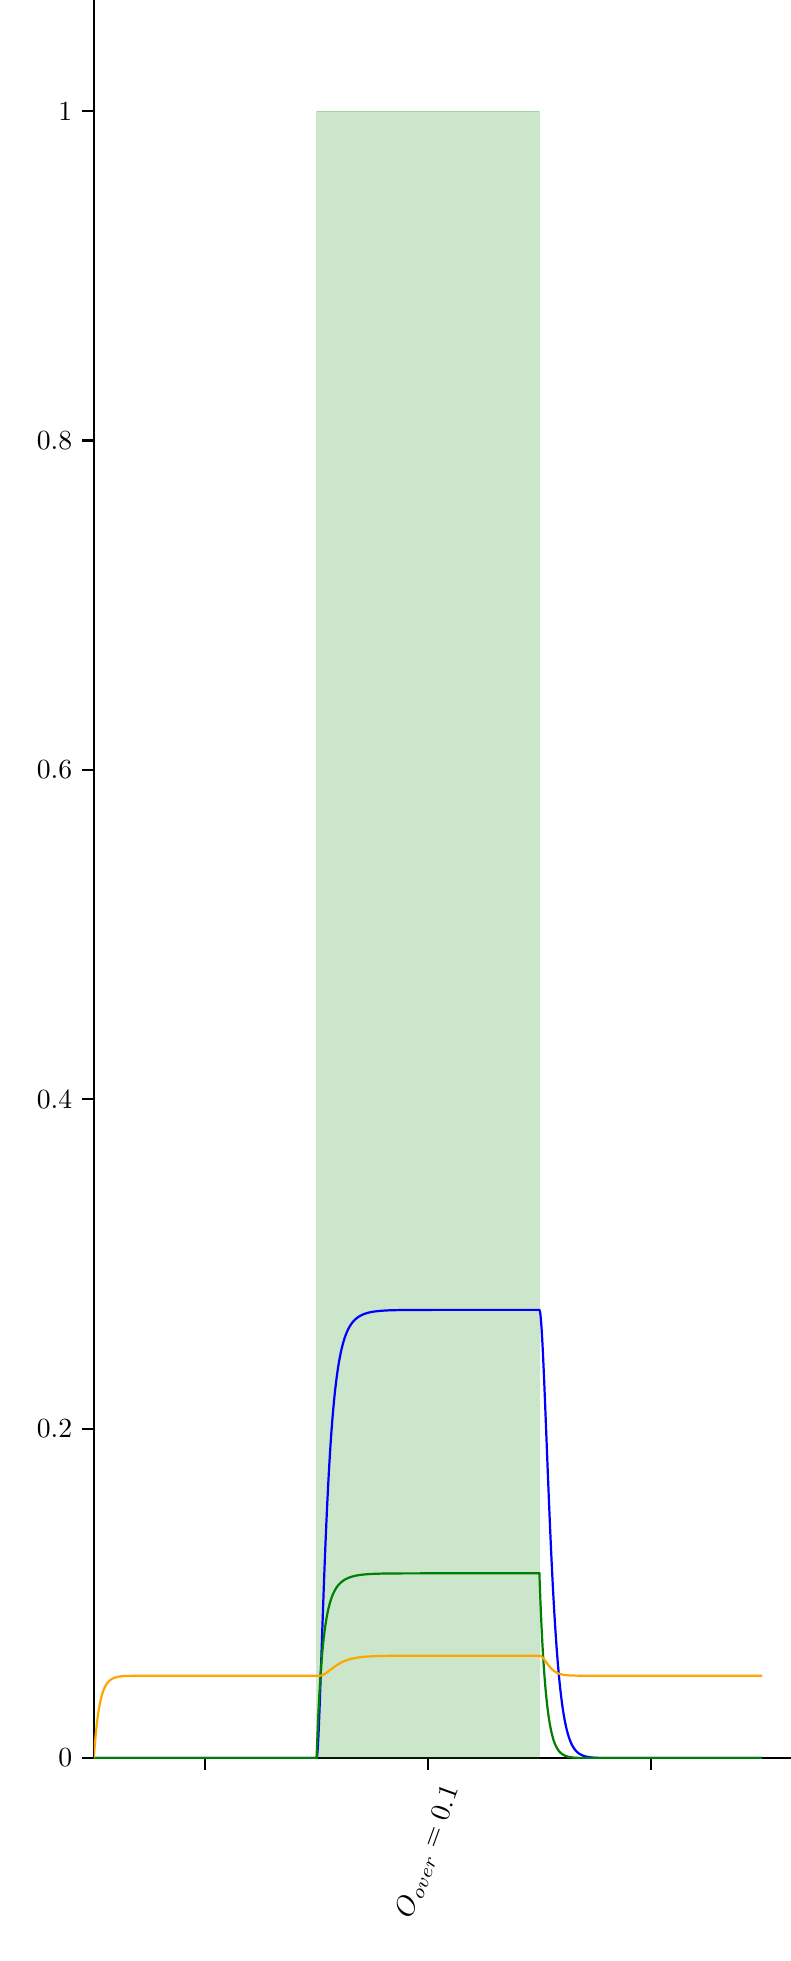
\begin{tikzpicture}[baseline]

\definecolor{darkgray176}{RGB}{176,176,176}
\definecolor{green}{RGB}{0,128,0}
\definecolor{lightgray204}{RGB}{204,204,204}
\definecolor{orange}{RGB}{255,165,0}

\begin{axis}[
 ytick={0,0.2,0.4,0.6,0.8,1},
 x tick label style = {rotate=70},
 y post scale=3, 
 transpose legend,
legend cell align={left},
legend style={fill opacity=0.8, draw opacity=1, text opacity=1, draw=lightgray204, anchor=south west,
    legend columns=4,
    /tikz/every even column/.append style={column sep=1.0cm},, at={(axis cs:5,1.1)}},
tick align=outside,
tick pos=left,
x grid style={darkgray176},
xmin=0, xmax=120,
xtick style={color=black},
xtick={20,60,100},
xticklabels={,\(\displaystyle O_\text{over}=0.1\),},
y grid style={darkgray176},
ymin=0, ymax=1.05,
ytick style={color=black}
]
\path [draw=green, fill=green, opacity=0.2]
(axis cs:40,0)
--(axis cs:40,1)
--(axis cs:80,1)
--(axis cs:80,0)
--cycle;

\addplot [thick, blue]
table {%
0 0
0.0001 0
0.0011 0
0.0111 0
0.1111 0
0.2111 0
0.3111 0
0.4111 0
0.5111 0
0.6111 0
0.7111 0
0.8111 0
0.9111 0
1.0111 0
1.1111 0
1.2111 0
1.3111 0
1.4111 0
1.5111 0
1.6111 0
1.7111 0
1.8111 0
1.9111 0
2.0111 0
2.1111 0
2.2111 0
2.3111 0
2.4111 0
2.5111 0
2.6111 0
2.7111 0
2.8111 0
2.9111 0
3.0111 0
3.1111 0
3.2111 0
3.3111 0
3.4111 0
3.5111 0
3.6111 0
3.7111 0
3.8111 0
3.9111 0
4.0111 0
4.1111 0
4.2111 0
4.3111 0
4.4111 0
4.5111 0
4.6111 0
4.7111 0
4.8111 0
4.9111 0
5.0111 0
5.1111 0
5.2111 0
5.3111 0
5.4111 0
5.5111 0
5.6111 0
5.7111 0
5.8111 0
5.9111 0
6.0111 0
6.1111 0
6.21109999999999 0
6.31109999999999 0
6.41109999999999 0
6.51109999999999 0
6.61109999999999 0
6.71109999999999 0
6.81109999999999 0
6.91109999999999 0
7.01109999999999 0
7.11109999999999 0
7.21109999999999 0
7.31109999999999 0
7.41109999999999 0
7.51109999999999 0
7.61109999999999 0
7.71109999999999 0
7.81109999999999 0
7.91109999999999 0
8.01109999999999 0
8.11109999999999 0
8.21109999999999 0
8.31109999999999 0
8.41109999999999 0
8.51109999999999 0
8.61109999999999 0
8.71109999999999 0
8.81109999999999 0
8.91109999999999 0
9.01109999999998 0
9.11109999999998 0
9.21109999999998 0
9.31109999999998 0
9.41109999999998 0
9.51109999999998 0
9.61109999999998 0
9.71109999999998 0
9.81109999999998 0
9.91109999999998 0
10.0111 0
10.1111 0
10.2111 0
10.3111 0
10.4111 0
10.5111 0
10.6111 0
10.7111 0
10.8111 0
10.9111 0
11.0111 0
11.1111 0
11.2111 0
11.3111 0
11.4111 0
11.5111 0
11.6111 0
11.7111 0
11.8111 0
11.9111 0
12.0111 0
12.1111 0
12.2111 0
12.3111 0
12.4111 0
12.5111 0
12.6111 0
12.7111 0
12.8111 0
12.9111 0
13.0111 0
13.1111 0
13.2111 0
13.3111 0
13.4111 0
13.5111 0
13.6111 0
13.7111 0
13.8111 0
13.9111 0
14.0111 0
14.1111 0
14.2111 0
14.3111 0
14.4111 0
14.5111 0
14.6111 0
14.7111 0
14.8111 0
14.9111 0
15.0111 0
15.1111 0
15.2111 0
15.3111 0
15.4111 0
15.5111 0
15.6111 0
15.7111 0
15.8111 0
15.9111 0
16.0111 0
16.1111 0
16.2111 0
16.3111 0
16.4111 0
16.5111 0
16.6111 0
16.7111 0
16.8111 0
16.9111 0
17.0111 0
17.1111 0
17.2111 0
17.3111 0
17.4111 0
17.5111 0
17.6111 0
17.7111 0
17.8111 0
17.9111 0
18.0111 0
18.1111 0
18.2111 0
18.3111 0
18.4111 0
18.5111 0
18.6111 0
18.7111 0
18.8111 0
18.9111 0
19.0111 0
19.1111 0
19.2111 0
19.3111 0
19.4111 0
19.5111 0
19.6111 0
19.7111 0
19.8111 0
19.9111 0
20.0111 0
20.1111 0
20.2111 0
20.3111 0
20.4111 0
20.5111 0
20.6111 0
20.7111 0
20.8111 0
20.9111 0
21.0111 0
21.1111 0
21.2111 0
21.3111 0
21.4111 0
21.5111 0
21.6111 0
21.7111 0
21.8111 0
21.9111 0
22.0111 0
22.1111 0
22.2111 0
22.3111 0
22.4111000000001 0
22.5111000000001 0
22.6111000000001 0
22.7111000000001 0
22.8111000000001 0
22.9111000000001 0
23.0111000000001 0
23.1111000000001 0
23.2111000000001 0
23.3111000000001 0
23.4111000000001 0
23.5111000000001 0
23.6111000000001 0
23.7111000000001 0
23.8111000000001 0
23.9111000000001 0
24.0111000000001 0
24.1111000000001 0
24.2111000000001 0
24.3111000000001 0
24.4111000000001 0
24.5111000000001 0
24.6111000000001 0
24.7111000000001 0
24.8111000000001 0
24.9111000000001 0
25.0111000000001 0
25.1111000000001 0
25.2111000000001 0
25.3111000000001 0
25.4111000000001 0
25.5111000000001 0
25.6111000000001 0
25.7111000000001 0
25.8111000000001 0
25.9111000000001 0
26.0111000000001 0
26.1111000000001 0
26.2111000000001 0
26.3111000000001 0
26.4111000000001 0
26.5111000000001 0
26.6111000000001 0
26.7111000000001 0
26.8111000000001 0
26.9111000000001 0
27.0111000000001 0
27.1111000000001 0
27.2111000000001 0
27.3111000000001 0
27.4111000000001 0
27.5111000000001 0
27.6111000000001 0
27.7111000000001 0
27.8111000000001 0
27.9111000000001 0
28.0111000000001 0
28.1111000000001 0
28.2111000000001 0
28.3111000000001 0
28.4111000000001 0
28.5111000000001 0
28.6111000000001 0
28.7111000000001 0
28.8111000000001 0
28.9111000000001 0
29.0111000000001 0
29.1111000000001 0
29.2111000000001 0
29.3111000000001 0
29.4111000000002 0
29.5111000000002 0
29.6111000000002 0
29.7111000000002 0
29.8111000000002 0
29.9111000000002 0
30.0111000000002 0
30.1111000000002 0
30.2111000000002 0
30.3111000000002 0
30.4111000000002 0
30.5111000000002 0
30.6111000000002 0
30.7111000000002 0
30.8111000000002 0
30.9111000000002 0
31.0111000000002 0
31.1111000000002 0
31.2111000000002 0
31.3111000000002 0
31.4111000000002 0
31.5111000000002 0
31.6111000000002 0
31.7111000000002 0
31.8111000000002 0
31.9111000000002 0
32.0111000000002 0
32.1111000000002 0
32.2111000000002 0
32.3111000000002 0
32.4111000000002 0
32.5111000000002 0
32.6111000000002 0
32.7111000000002 0
32.8111000000002 0
32.9111000000002 0
33.0111000000002 0
33.1111000000002 0
33.2111000000002 0
33.3111000000002 0
33.4111000000002 0
33.5111000000002 0
33.6111000000002 0
33.7111000000002 0
33.8111000000002 0
33.9111000000002 0
34.0111000000002 0
34.1111000000002 0
34.2111000000002 0
34.3111000000002 0
34.4111000000002 0
34.5111000000002 0
34.6111000000002 0
34.7111000000002 0
34.8111000000002 0
34.9111000000002 0
35.0111000000002 0
35.1111000000002 0
35.2111000000002 0
35.3111000000002 0
35.4111000000002 0
35.5111000000002 0
35.6111000000002 0
35.7111000000002 0
35.8111000000002 0
35.9111000000002 0
36.0111000000002 0
36.1111000000002 0
36.2111000000002 0
36.3111000000002 0
36.4111000000002 0
36.5111000000002 0
36.6111000000002 0
36.7111000000003 0
36.8111000000003 0
36.9111000000003 0
37.0111000000003 0
37.1111000000003 0
37.2111000000003 0
37.3111000000003 0
37.4111000000003 0
37.5111000000003 0
37.6111000000003 0
37.7111000000003 0
37.8111000000003 0
37.9111000000003 0
38.0111000000003 0
38.1111000000003 0
38.2111000000003 0
38.3111000000003 0
38.4111000000003 0
38.5111000000003 0
38.6111000000003 0
38.7111000000003 0
38.8111000000003 0
38.9111000000003 0
39.0111000000003 0
39.1111000000003 0
39.2111000000003 0
39.3111000000003 0
39.4111000000003 0
39.5111000000003 0
39.6111000000003 0
39.7111000000003 0
39.8111000000003 0
39.9111000000003 0
40 0
40 0
40.0098039215686 1.58806847940183e-05
40.1078431372549 0.00176379699809601
40.2078431372549 0.00601744468822837
40.3078431372549 0.0121515011732288
40.4078431372549 0.0196731086821273
40.5078431372549 0.028189821408099
40.6078431372549 0.0373893489625429
40.7078431372549 0.0470236816628587
40.8078431372549 0.0568964940423887
40.9078431372549 0.0668530835289466
41.0078431372549 0.0767723092505508
41.1078431372549 0.0865601224031734
41.2078431372549 0.0961443654431092
41.3078431372549 0.10547058222457
41.4078431372549 0.114498633257489
41.5078431372549 0.123199952697904
41.6078431372549 0.131555318030718
41.7078431372549 0.13955303082015
41.8078431372549 0.147187428507448
41.9078431372549 0.154457664108385
42.0078431372549 0.16136670377903
42.1078431372549 0.167920502403903
42.2078431372549 0.174127325286196
42.3078431372549 0.179997190212196
42.4078431372549 0.185541409027456
42.5078431372549 0.190772211709523
42.6078431372549 0.195702438985283
42.7078431372549 0.200345291996744
42.8078431372549 0.204714129501368
42.9078431372549 0.20882230470334
43.0078431372549 0.212683035128259
43.1078431372549 0.216309300035266
43.2078431372549 0.219713760753948
43.3078431372549 0.222908700074489
43.4078431372549 0.225905977436994
43.5078431372549 0.22871699718203
43.6078431372549 0.231352687557313
43.7078431372549 0.233823488539399
43.8078431372549 0.236139346836029
43.9078431372549 0.238309716693749
44.0078431372549 0.24034356535453
44.1078431372549 0.242249382190609
44.2078431372549 0.244035190704
44.3078431372549 0.245708562710507
44.4078431372549 0.247276634141207
44.5078431372549 0.248746121990383
44.6078431372549 0.250123342020354
44.7078431372549 0.251414226902675
44.8078431372549 0.252624344533712
44.907843137255 0.253758916312093
45.007843137255 0.254822835207377
45.107843137255 0.255820683484572
45.207843137255 0.256756749978804
45.307843137255 0.257635046839399
45.407843137255 0.258459325683454
45.507843137255 0.259233093116365
45.607843137255 0.259959625591185
45.707843137255 0.260641983590575
45.807843137255 0.261283025124863
45.907843137255 0.261885418547622
46.007843137255 0.262451654696587
46.107843137255 0.262984058372777
46.207843137255 0.263484799174651
46.307843137255 0.26395590170717
46.407843137255 0.264399255187904
46.507843137255 0.264816622473897
46.607843137255 0.26520964853411
46.707843137255 0.26557986839284
46.807843137255 0.265928714569805
46.907843137255 0.2662575240425
47.007843137255 0.26656754475616
47.107843137255 0.266859941706198
47.207843137255 0.267135802617322
47.307843137255 0.267396143242821
47.407843137255 0.267641912306658
47.507843137255 0.267873996110132
47.607843137255 0.268093222823914
47.707843137255 0.268300366485326
47.807843137255 0.268496150719756
47.907843137255 0.268681252204129
48.007843137255 0.268856303889408
48.107843137255 0.269021897998156
48.207843137255 0.269178588812279
48.307843137255 0.26932689526517
48.407843137255 0.269467303351654
48.507843137255 0.269600268368257
48.607843137255 0.269726216995601
48.707843137255 0.26984554923392
48.807843137255 0.269958640202016
48.907843137255 0.270065841809287
49.007843137255 0.270167484309808
49.107843137255 0.270263877746862
49.207843137255 0.270355313295724
49.307843137255 0.270442064511993
49.407843137255 0.270524388492235
49.507843137255 0.270602526953249
49.607843137255 0.270676707235806
49.707843137255 0.270747143238317
49.807843137255 0.270814036285485
49.907843137255 0.270877575936627
50.007843137255 0.270937940738046
50.107843137255 0.270995298923469
50.207843137255 0.271049809066325
50.307843137255 0.271101620687333
50.407843137255 0.271150874820611
50.507843137255 0.271197704541322
50.607843137255 0.271242235457594
50.707843137255 0.271284586169304
50.807843137255 0.271324868696087
50.907843137255 0.271363188876787
51.007843137255 0.271399646742368
51.107843137255 0.27143433686419
51.207843137255 0.271467348679403
51.307843137255 0.271498766795054
51.407843137255 0.271528671272437
51.507843137255 0.271557137893057
51.607843137255 0.271584238407501
51.707843137255 0.271610040768406
51.807843137255 0.271634609348635
51.907843137255 0.271658005145677
52.0078431372551 0.271680285973221
52.1078431372551 0.271701506640788
52.2078431372551 0.271721719122226
52.3078431372551 0.271740972713836
52.4078431372551 0.271759314182822
52.5078431372551 0.271776787906707
52.6078431372551 0.27179343600434
52.7078431372551 0.27180929845903
52.8078431372551 0.271824413234337
52.9078431372551 0.271838816383007
53.0078431372551 0.27185254214949
53.1078431372551 0.271865623066454
53.2078431372551 0.271878090045699
53.3078431372551 0.271889972463812
53.4078431372551 0.271901298242904
53.5078431372551 0.271912093926746
53.6078431372551 0.271922384752586
53.7078431372551 0.271932194718913
53.8078431372551 0.271941546649435
53.9078431372551 0.271950462253485
54.0078431372551 0.271958962183093
54.1078431372551 0.271967066086904
54.2078431372551 0.271974792661159
54.3078431372551 0.271982159697891
54.4078431372551 0.271989184130518
54.5078431372551 0.271995882076981
54.6078431372551 0.272002268880573
54.7078431372551 0.272008359148585
54.8078431372551 0.272014166788922
54.9078431372551 0.272019705044765
55.0078431372551 0.272024986527434
55.1078431372551 0.272030023247522
55.2078431372551 0.272034826644416
55.3078431372551 0.272039407614286
55.4078431372551 0.272043776536639
55.5078431372551 0.2720479432995
55.6078431372551 0.272051917323317
55.7078431372551 0.27205570758364
55.8078431372551 0.272059322632656
55.9078431372551 0.272062770619636
56.0078431372551 0.272066059310353
56.1078431372551 0.272069196105521
56.2078431372551 0.272072188058321
56.3078431372551 0.272075041891051
56.4078431372551 0.272077764010945
56.5078431372551 0.272080360525218
56.6078431372551 0.272082837255358
56.7078431372551 0.27208519975073
56.8078431372551 0.272087453301492
56.9078431372551 0.272089602950901
57.0078431372551 0.272091653507002
57.1078431372551 0.272093609553759
57.2078431372551 0.272095475461636
57.3078431372551 0.272097255397676
57.4078431372551 0.272098953335084
57.5078431372551 0.272100573062352
57.6078431372551 0.272102118191943
57.7078431372551 0.272103592168565
57.8078431372551 0.272104998277035
57.9078431372551 0.272106339649778
58.0078431372551 0.272107619273967
58.1078431372551 0.272108839998312
58.2078431372551 0.272110004539544
58.3078431372551 0.27211111548857
58.4078431372551 0.272112175316355
58.5078431372551 0.272113186379512
58.6078431372551 0.272114150925633
58.7078431372551 0.272115071098369
58.8078431372551 0.272115948942264
58.9078431372551 0.272116786407373
59.0078431372552 0.272117585353647
59.1078431372552 0.272118347555127
59.2078431372552 0.27211907470393
59.3078431372552 0.272119768414052
59.4078431372552 0.272120430224994
59.5078431372552 0.272121061605216
59.6078431372552 0.27212166395543
59.7078431372552 0.272122238611738
59.8078431372552 0.272122786848628
59.9078431372552 0.272123309881821
60.0078431372552 0.272123808870997
60.1078431372552 0.272124284922382
60.2078431372552 0.272124739091224
60.3078431372552 0.272125172384149
60.4078431372552 0.272125585761407
60.5078431372552 0.272125980139015
60.6078431372552 0.272126356390803
60.7078431372552 0.272126715350359
60.8078431372552 0.272127057812886
60.9078431372552 0.27212738453698
61.0078431372552 0.272127696246313
61.1078431372552 0.272127993631244
61.2078431372552 0.272128277350363
61.3078431372552 0.272128548031946
61.4078431372552 0.272128806275361
61.5078431372552 0.272129052652398
61.6078431372552 0.272129287708537
61.7078431372552 0.272129511964165
61.8078431372552 0.272129725915729
61.9078431372552 0.272129930036843
62.0078431372552 0.272130124779334
62.1078431372552 0.27213031057425
62.2078431372552 0.272130487832815
62.3078431372552 0.272130656947343
62.4078431372552 0.272130818292107
62.5078431372552 0.272130972224172
62.6078431372552 0.272131119084182
62.7078431372552 0.272131259197124
62.8078431372552 0.27213139287304
62.9078431372552 0.272131520407721
63.0078431372552 0.272131642083358
63.1078431372552 0.272131758169173
63.2078431372552 0.272131868922009
63.3078431372552 0.272131974586907
63.4078431372552 0.272132075397643
63.5078431372552 0.272132171577247
63.6078431372552 0.2721322633385
63.7078431372552 0.272132350884405
63.8078431372552 0.272132434408631
63.9078431372552 0.272132514095952
64.0078431372552 0.272132590122646
64.1078431372552 0.272132662656893
64.2078431372552 0.272132731859144
64.3078431372552 0.272132797882476
64.4078431372552 0.272132860872933
64.5078431372552 0.272132920969848
64.6078431372552 0.27213297830615
64.7078431372552 0.272133033008663
64.8078431372552 0.272133085198381
64.9078431372552 0.272133134990741
65.0078431372552 0.272133182495874
65.1078431372552 0.272133227818853
65.2078431372552 0.272133271059921
65.3078431372551 0.272133312314718
65.4078431372551 0.272133351674488
65.5078431372551 0.272133389226283
65.6078431372551 0.272133425053157
65.7078431372551 0.272133459234348
65.8078431372551 0.272133491845451
65.9078431372551 0.272133522958593
66.0078431372551 0.272133552642583
66.1078431372551 0.27213358096307
66.2078431372551 0.27213360798269
66.3078431372551 0.272133633761196
66.4078431372551 0.272133658355602
66.5078431372551 0.272133681820298
66.6078431372551 0.272133704207179
66.7078431372551 0.272133725565753
66.8078431372551 0.272133745943256
66.9078431372551 0.272133765384753
67.0078431372551 0.272133783933239
67.107843137255 0.272133801629733
67.207843137255 0.272133818513373
67.307843137255 0.272133834621494
67.407843137255 0.272133849989721
67.507843137255 0.27213386465204
67.607843137255 0.272133878640875
67.707843137255 0.272133891987163
67.807843137255 0.272133904720417
67.907843137255 0.272133916868798
68.007843137255 0.27213392845917
68.107843137255 0.272133939517164
68.207843137255 0.272133950067235
68.307843137255 0.272133960132712
68.407843137255 0.272133969735856
68.507843137255 0.272133978897903
68.607843137255 0.272133987639113
68.707843137255 0.272133995978816
68.8078431372549 0.272134003935456
68.9078431372549 0.272134011526628
69.0078431372549 0.272134018769118
69.1078431372549 0.272134025678943
69.2078431372549 0.272134032271383
69.3078431372549 0.272134038561016
69.4078431372549 0.272134044561751
69.5078431372549 0.272134050286858
69.6078431372549 0.272134055748998
69.7078431372549 0.272134060960248
69.8078431372549 0.272134065932134
69.9078431372549 0.272134070675649
70.0078431372549 0.272134075201284
70.1078431372549 0.272134079519046
70.2078431372549 0.272134083638483
70.3078431372549 0.272134087568705
70.4078431372549 0.272134091318403
70.5078431372549 0.272134094895869
70.6078431372548 0.272134098309014
70.7078431372548 0.272134101565386
70.8078431372548 0.272134104672186
70.9078431372548 0.272134107636283
71.0078431372548 0.272134110464232
71.1078431372548 0.272134113162288
71.2078431372548 0.272134115736416
71.3078431372548 0.272134118192309
71.4078431372548 0.272134120535398
71.5078431372548 0.272134122770863
71.6078431372548 0.272134124903648
71.7078431372548 0.272134126938471
71.8078431372548 0.272134128879829
71.9078431372548 0.272134130732017
72.0078431372548 0.272134132499129
72.1078431372548 0.272134134185075
72.2078431372548 0.272134135793581
72.3078431372547 0.272134137328205
72.4078431372547 0.272134138792341
72.5078431372547 0.272134140189226
72.6078431372547 0.272134141521949
72.7078431372547 0.272134142793457
72.8078431372547 0.272134144006562
72.9078431372547 0.272134145163947
73.0078431372547 0.272134146268171
73.1078431372547 0.272134147321675
73.2078431372547 0.27213414832679
73.3078431372547 0.272134149285737
73.4078431372547 0.272134150200639
73.5078431372547 0.272134151073516
73.6078431372547 0.272134151906301
73.7078431372547 0.272134152700834
73.8078431372547 0.272134153458873
73.9078431372547 0.272134154182094
74.0078431372547 0.272134154872095
74.1078431372546 0.272134155530403
74.2078431372546 0.272134156158474
74.3078431372546 0.272134156757696
74.4078431372546 0.272134157329395
74.5078431372546 0.272134157874834
74.6078431372546 0.27213415839522
74.7078431372546 0.272134158891704
74.8078431372546 0.272134159365383
74.9078431372546 0.272134159817305
75.0078431372546 0.27213416024847
75.1078431372546 0.27213416065983
75.2078431372546 0.272134161052296
75.3078431372546 0.272134161426735
75.4078431372546 0.272134161783975
75.5078431372546 0.272134162124806
75.6078431372546 0.272134162449982
75.7078431372546 0.272134162760223
75.8078431372546 0.272134163056213
75.9078431372545 0.272134163338608
76.0078431372545 0.272134163608031
76.1078431372545 0.27213416386508
76.2078431372545 0.272134164110322
76.3078431372545 0.272134164344299
76.4078431372545 0.27213416456753
76.5078431372545 0.272134164780507
76.6078431372545 0.272134164983701
76.7078431372545 0.272134165177563
76.8078431372545 0.27213416536252
76.9078431372545 0.272134165538981
77.0078431372545 0.272134165707337
77.1078431372545 0.272134165867961
77.2078431372545 0.272134166021206
77.3078431372545 0.272134166167413
77.4078431372545 0.272134166306904
77.5078431372545 0.272134166439988
77.6078431372544 0.272134166566959
77.7078431372544 0.272134166688098
77.8078431372544 0.272134166803673
77.9078431372544 0.272134166913939
78.0078431372544 0.272134167019141
78.1078431372544 0.27213416711951
78.2078431372544 0.27213416721527
78.3078431372544 0.27213416730663
78.4078431372544 0.272134167393795
78.5078431372544 0.272134167476956
78.6078431372544 0.272134167556297
78.7078431372544 0.272134167631994
78.8078431372544 0.272134167704213
78.9078431372544 0.272134167773116
79.0078431372544 0.272134167838854
79.1078431372544 0.272134167901572
79.2078431372544 0.27213416796141
79.3078431372544 0.272134168018499
79.4078431372543 0.272134168072966
79.5078431372543 0.272134168124931
79.6078431372543 0.272134168174509
79.7078431372543 0.27213416822181
79.8078431372543 0.272134168266939
79.9078431372543 0.272134168309994
80 0.27213416834792
80 0.27213416834792
80.1 0.271292422770216
80.2 0.268924191293731
80.3 0.265247959716204
80.4 0.260460951297077
80.5 0.254740823833699
80.6 0.248247255234674
80.7 0.241123419228688
80.8 0.233497354025907
80.8999999999999 0.225483228091181
80.9999999999999 0.217182508408273
81.0999999999999 0.208685037544137
81.1999999999999 0.200070026388486
81.2999999999999 0.191406969642392
81.3999999999999 0.182756491003045
81.4999999999999 0.174171124608632
81.5999999999999 0.165696038746217
81.6999999999999 0.157369707163132
81.7999999999999 0.149224532625833
81.8999999999999 0.141287426692492
81.9999999999999 0.133580349044757
82.0999999999999 0.126120809183563
82.1999999999999 0.118922332844407
82.2999999999999 0.111994895130138
82.3999999999999 0.105345322087807
82.4999999999999 0.0989776622598187
82.5999999999999 0.092893529605527
82.6999999999998 0.0870924191040161
82.7999999999998 0.0815719962993591
82.8999999999998 0.0763283620248213
82.9999999999998 0.0713562935329854
83.0999999999998 0.0666494632572418
83.1999999999998 0.0622006364311028
83.2999999999998 0.0580018487915615
83.3999999999998 0.0540445655888116
83.4999999999998 0.050319823115648
83.5999999999998 0.0468183539551218
83.6999999999998 0.0435306971243624
83.7999999999998 0.0404472942660526
83.8999999999998 0.0375585730072046
83.9999999999998 0.0348550185680884
84.0999999999998 0.0323272346629566
84.1999999999998 0.029965994689143
84.2999999999998 0.0277622841528143
84.3999999999997 0.0257073352287466
84.4999999999997 0.0237926542986329
84.5999999999997 0.0220100432582614
84.6999999999997 0.0203516153290854
84.7999999999997 0.0188098060548661
84.8999999999997 0.0173773801097903
84.9999999999997 0.016047434491298
85.0999999999997 0.0148133986192686
85.1999999999997 0.0136690318136194
85.2999999999997 0.0126084185750977
85.3999999999997 0.0116259620493588
85.4999999999997 0.0107163760124903
85.5999999999997 0.00987467567709659
85.6999999999997 0.00909616758193522
85.7999999999997 0.00837643879490559
85.8999999999997 0.00771134562888116
85.9999999999997 0.00709700204235808
86.0999999999997 0.00652976787205684
86.1999999999996 0.00600623702231758
86.2999999999996 0.00552322571622269
86.3999999999996 0.00507776089569878
86.4999999999996 0.00466706884222787
86.5999999999996 0.00428856407606548
86.6999999999996 0.0039398385798578
86.7999999999996 0.00361865138210943
86.8999999999996 0.00332291852692635
86.9999999999996 0.00305070344870028
87.0999999999996 0.00280020776377514
87.1999999999996 0.00256976248551991
87.2999999999996 0.00235781966450692
87.3999999999996 0.00216294445155727
87.4999999999996 0.0019838075781671
87.5999999999996 0.00181917824618458
87.6999999999996 0.00166791741648778
87.7999999999996 0.00152897148474893
87.8999999999996 0.0014013663310971
87.9999999999995 0.00128420172955403
88.0999999999995 0.00117664610246647
88.1999999999995 0.00107793160475005
88.2999999999995 0.000987349522555197
88.3999999999995 0.000904245970931628
88.4999999999995 0.000828017875175431
88.5999999999995 0.000758109220765145
88.6999999999995 0.000694007557109388
88.7999999999995 0.000635240740718632
88.8999999999995 0.00058137390386145
88.9999999999995 0.000532006635256802
89.0999999999995 0.000486770359876702
89.1999999999995 0.000445325905477594
89.2999999999995 0.000407361244035548
89.3999999999995 0.000372589396822631
89.4999999999995 0.000340746492423608
89.5999999999995 0.000311589967548631
89.6999999999994 0.000284896901044644
89.7999999999994 0.000260462472042872
89.8999999999994 0.000238098533699261
89.9999999999994 0.000217632294487314
90.0999999999994 0.000198905099486859
90.1999999999994 0.000181771304577015
90.2999999999994 0.000166097236886168
90.3999999999994 0.000151760235275892
90.4999999999994 0.000138647765039288
90.5999999999994 0.000126656601377242
90.6999999999994 0.000115692076578898
90.7999999999994 0.000105667386175589
90.8999999999994 9.6502949661066e-05
90.9999999999994 8.81258216756869e-05
91.0999999999994 8.04691498389417e-05
91.1999999999994 7.34716756839558e-05
91.2999999999994 6.70772754001834e-05
91.3999999999994 6.12345373271077e-05
91.4999999999993 5.58963733631536e-05
91.5999999999993 5.10196616609597e-05
91.6999999999993 4.65649181733756e-05
91.7999999999993 4.24959947948103e-05
91.8999999999993 3.87798020105527e-05
91.9999999999993 3.53860541231341e-05
92.0999999999993 3.22870352703752e-05
92.1999999999993 2.94573845851095e-05
92.2999999999993 2.6873898972333e-05
92.3999999999993 2.45153520962928e-05
92.4999999999993 2.23623282783686e-05
92.5999999999993 2.03970701070712e-05
92.6999999999993 1.86033386545908e-05
92.7999999999993 1.69662852805712e-05
92.8999999999993 1.54723340836293e-05
92.9999999999993 1.41090741350121e-05
93.0999999999993 1.28651606971083e-05
93.1999999999992 1.17302246926888e-05
93.2999999999992 1.06947897491082e-05
93.3999999999992 9.75019619559652e-06
93.4999999999992 8.88853144153226e-06
93.5999999999992 8.10256620950733e-06
93.6999999999992 7.38569613935617e-06
93.7999999999992 6.73188831838638e-06
93.8999999999992 6.1356323290585e-06
93.9999999999992 5.59189543854761e-06
94.0999999999992 5.09608158518974e-06
94.1999999999992 4.64399384496931e-06
94.2999999999992 4.2318000871231e-06
94.3999999999992 3.85600155179153e-06
94.4999999999992 3.51340410459778e-06
94.5999999999992 3.20109194322592e-06
94.6999999999992 2.91640354963678e-06
94.7999999999992 2.65690969863121e-06
94.8999999999992 2.42039334916041e-06
94.9999999999991 2.20483125920195e-06
95.0999999999991 2.00837717826586e-06
95.1999999999991 1.82934648376228e-06
95.2999999999991 1.66620213863463e-06
95.3999999999991 1.51754185792e-06
95.4999999999991 1.38208638131383e-06
95.5999999999991 1.25866875745715e-06
95.6999999999991 1.14622455359255e-06
95.7999999999991 1.04378291150865e-06
95.8999999999991 9.50458377363629e-07
95.9999999999991 8.65443439095526e-07
96.0999999999991 7.88001710736479e-07
96.1999999999991 7.17461708089165e-07
96.2999999999991 6.53211164936689e-07
96.3999999999991 5.94691843275759e-07
96.4999999999991 5.41394795019985e-07
96.5999999999991 4.9285603624528e-07
96.6999999999991 4.48652598369848e-07
96.799999999999 4.08398923702264e-07
96.899999999999 3.71743575575954e-07
96.999999999999 3.38366235837944e-07
97.099999999999 3.07974964793908e-07
97.199999999999 2.80303700847947e-07
97.299999999999 2.55109979030878e-07
97.399999999999 2.32172849400095e-07
97.499999999999 2.11290977931232e-07
97.599999999999 1.92280914019629e-07
97.699999999999 1.74975510079752e-07
97.799999999999 1.59222479983844e-07
97.899999999999 1.44883084227193e-07
97.999999999999 1.31830930755405e-07
98.099999999999 1.19950881347332e-07
98.199999999999 1.09138054323368e-07
98.299999999999 9.92969151496662e-08
98.399999999999 9.03404472408757e-08
98.4999999999989 8.21893959330021e-08
98.5999999999989 7.47715792094271e-08
98.6999999999989 6.80212593217948e-08
98.7999999999989 6.18785699579482e-08
98.8999999999989 5.62889940754642e-08
98.9999999999989 5.12028879453682e-08
99.0999999999989 4.65750473397633e-08
99.1999999999989 4.23643121525491e-08
99.2999999999989 3.85332060670129e-08
99.3999999999989 3.50476081805154e-08
99.4999999999989 3.18764537671701e-08
99.5999999999989 2.89914616065643e-08
99.6999999999989 2.63668855322021e-08
99.7999999999989 2.39792880593374e-08
99.8999999999989 2.18073341398876e-08
99.9999999999989 1.98316032637479e-08
100.099999999999 1.8034418282461e-08
100.199999999999 1.63996894741539e-08
100.299999999999 1.49127724991017e-08
100.399999999999 1.35603390143194e-08
100.499999999999 1.23302588241917e-08
100.599999999999 1.12114925432461e-08
100.699999999999 1.01939938375788e-08
100.799999999999 9.26862039391002e-09
100.899999999999 8.42705284047721e-09
100.999999999999 7.66172091258564e-09
101.099999999999 6.96573621822336e-09
101.199999999999 6.33283101621971e-09
101.299999999999 5.75730247147863e-09
101.399999999999 5.23396189928117e-09
101.499999999999 4.75808855393204e-09
101.599999999999 4.32538755648636e-09
101.699999999999 3.93195159227178e-09
101.799999999999 3.57422604172206e-09
101.899999999999 3.24897723794053e-09
101.999999999999 2.95326357167045e-09
102.099999999999 2.68440918919579e-09
102.199999999999 2.4399800513437e-09
102.299999999999 2.21776214240112e-09
102.399999999999 2.01574163657039e-09
102.499999999999 1.83208684673341e-09
102.599999999999 1.66513179591679e-09
102.699999999999 1.513361266088e-09
102.799999999999 1.37539719188436e-09
102.899999999999 1.24998627869747e-09
102.999999999999 1.13598873530445e-09
103.099999999999 1.03236802104947e-09
103.199999999999 9.3818151651736e-10
103.299999999999 8.52572034784228e-10
103.399999999999 7.74760097747743e-10
103.499999999999 7.04036908796579e-10
103.599999999999 6.39757959233044e-10
103.699999999999 5.81337211468671e-10
103.799999999999 5.28241807118039e-10
103.899999999999 4.79987252766002e-10
103.999999999999 4.36133040418101e-10
104.099999999999 3.9627866350032e-10
104.199999999999 3.60059992786024e-10
104.299999999999 3.2714597982564e-10
104.399999999999 2.97235658366403e-10
104.499999999999 2.70055416900596e-10
104.599999999999 2.45356517894625e-10
104.699999999999 2.22912841448914e-10
104.799999999999 2.02518833139471e-10
104.899999999999 1.83987637613414e-10
104.999999999999 1.67149401169002e-10
105.099999999999 1.51849728060164e-10
105.199999999999 1.37948276639573e-10
105.299999999999 1.25317482705065e-10
105.399999999999 1.13841398552602e-10
105.499999999999 1.03414637275191e-10
105.599999999999 9.39414127902374e-11
105.699999999999 8.53346669361531e-11
105.799999999999 7.75152757601722e-11
105.899999999999 7.04113278302431e-11
105.999999999999 6.39574680507903e-11
106.099999999999 5.80943010508601e-11
106.199999999999 5.27678487488763e-11
106.299999999999 4.7929057185701e-11
106.399999999998 4.35333481612513e-11
106.499999999998 3.95402116135059e-11
106.599999999998 3.59128350459421e-11
106.699999999998 3.26177666435352e-11
106.799999999998 2.9624609021415e-11
106.899999999998 2.69057408268064e-11
106.999999999998 2.44360636664601e-11
107.099999999998 2.2192772060646e-11
107.199999999998 2.01551443329775e-11
107.299999999998 1.83043525347304e-11
107.399999999998 1.66232896745967e-11
107.499999999998 1.50964126815234e-11
107.599999999998 1.37095996708266e-11
107.699999999998 1.24500202134247e-11
107.799999999998 1.13060174259547e-11
107.899999999998 1.02670008067919e-11
107.999999999998 9.32334884053854e-12
108.099999999998 8.46632048226582e-12
108.199999999998 7.68797471347185e-12
108.299999999998 6.98109743509844e-12
108.399999999998 6.33913502967329e-12
108.499999999998 5.75613398532616e-12
108.599999999998 5.22668602960774e-12
108.699999999998 4.74587827121682e-12
108.799999999998 4.30924789336853e-12
108.899999999998 3.91274098402411e-12
108.999999999998 3.55267512592645e-12
109.099999999998 3.2257054036859e-12
109.199999999998 2.92879351634701e-12
109.299999999998 2.65917971222229e-12
109.399999999998 2.41435728855835e-12
109.499999999998 2.19204942203833e-12
109.599999999998 1.9901881174325e-12
109.699999999998 1.80689508108135e-12
109.799999999998 1.64046434350632e-12
109.899999999998 1.48934647145327e-12
109.999999999998 1.35213422422795e-12
110.099999999998 1.22754952241266e-12
110.199999999998 1.11443160908007e-12
110.299999999998 1.0117262945521e-12
110.399999999998 9.18476185689185e-13
110.499999999998 8.33811809727399e-13
110.599999999998 7.56943550891393e-13
110.699999999998 6.87154325473124e-13
110.799999999998 6.23792927849188e-13
110.899999999998 5.66267986074106e-13
110.999999999998 5.14042471289841e-13
111.099999999998 4.6662871028403e-13
111.199999999998 4.235838551574e-13
111.299999999998 3.84505768266837e-13
111.399999999998 3.49029284433035e-13
111.499999999998 3.16822815875379e-13
111.599999999998 2.87585268493592e-13
111.699999999998 2.61043240984447e-13
111.799999999998 2.3694848088881e-13
111.899999999998 2.15075574033278e-13
111.999999999998 1.9521984598337e-13
112.099999999998 1.77195456081358e-13
112.199999999998 1.60833666419318e-13
112.299999999998 1.45981269713036e-13
112.399999999998 1.32499161509997e-13
112.499999999998 1.2026104349808e-13
112.599999999998 1.09152245893166e-13
112.699999999998 9.90686579846697e-14
112.799999999998 8.99157569181878e-14
112.899999999998 8.16077257031537e-14
112.999999999998 7.4066652259e-14
113.099999999998 6.7221802063411e-14
113.199999999998 6.10089576477073e-14
113.299999999998 5.53698188035074e-14
113.399999999998 5.02514579272581e-14
113.499999999998 4.56058254401885e-14
113.599999999998 4.13893006854282e-14
113.699999999998 3.75622841257185e-14
113.799999999998 3.40888270482113e-14
113.899999999998 3.09362953308373e-14
113.999999999998 2.80750641408327e-14
114.099999999998 2.547824072316e-14
114.199999999998 2.31214126973934e-14
114.299999999998 2.09824195185719e-14
114.399999999998 1.90411449727367e-14
114.499999999998 1.72793287733534e-14
114.599999999998 1.56803955023851e-14
114.699999999998 1.42292993010591e-14
114.799999999998 1.29123828618584e-14
114.899999999998 1.17172494063255e-14
114.999999999998 1.06326464541053e-14
115.099999999998 9.64836029841839e-15
115.199999999998 8.75512020283793e-15
115.299999999998 7.94451142478371e-15
115.399999999998 7.20889625337262e-15
115.499999999998 6.5413423239439e-15
115.599999999998 5.93555753939965e-15
115.699999999998 5.38583099009499e-15
115.799999999998 4.88697931994983e-15
115.899999999998 4.434298037254e-15
115.999999999998 4.02351731476997e-15
116.099999999998 3.65076186563236e-15
116.199999999998 3.31251451958796e-15
116.299999999998 3.00558315866909e-15
116.399999999998 2.72707070276594e-15
116.499999999998 2.4743478640533e-15
116.599999999998 2.24502841509715e-15
116.699999999998 2.03694673895813e-15
116.799999999998 1.84813745094063e-15
116.899999999998 1.67681690100543e-15
116.999999999998 1.52136638345209e-15
117.099999999998 1.38031689644737e-15
117.199999999998 1.25233530847666e-15
117.299999999998 1.13621180196196e-15
117.399999999998 1.03084847624507e-15
117.499999999998 9.35249002989016e-16
117.599999999998 8.48509236906644e-16
117.699999999998 7.69808693673256e-16
117.799999999998 6.98402815004904e-16
117.899999999998 6.33615948260186e-16
117.999999999998 5.74834974620553e-16
118.099999999998 5.21503525984476e-16
118.199999999998 4.73116736231052e-16
118.299999999998 4.29216477520455e-16
118.399999999998 3.89387036848618e-16
118.499999999998 3.53251192204356e-16
118.599999999998 3.20466651427302e-16
118.699999999998 2.90722820269547e-16
118.799999999998 2.63737869254652e-16
118.899999999998 2.39256071733534e-16
118.999999999998 2.17045388083917e-16
119.099999999998 1.96895273312385e-16
119.199999999998 1.78614687417177e-16
119.299999999998 1.62030289775445e-16
119.399999999998 1.46984800548455e-16
119.499999999998 1.33335513668518e-16
119.599999999998 1.20952947396789e-16
119.699999999998 1.09719619735015e-16
119.799999999998 9.95289371488274e-17
119.899999999998 9.02841861262868e-17
119.999999999998 8.18976180631989e-17
120 8.18976180630173e-17
};
\addplot [thick, green]
table {%
0 0
0.0001 0
0.0011 0
0.0111 0
0.1111 0
0.2111 0
0.3111 0
0.4111 0
0.5111 0
0.6111 0
0.7111 0
0.8111 0
0.9111 0
1.0111 0
1.1111 0
1.2111 0
1.3111 0
1.4111 0
1.5111 0
1.6111 0
1.7111 0
1.8111 0
1.9111 0
2.0111 0
2.1111 0
2.2111 0
2.3111 0
2.4111 0
2.5111 0
2.6111 0
2.7111 0
2.8111 0
2.9111 0
3.0111 0
3.1111 0
3.2111 0
3.3111 0
3.4111 0
3.5111 0
3.6111 0
3.7111 0
3.8111 0
3.9111 0
4.0111 0
4.1111 0
4.2111 0
4.3111 0
4.4111 0
4.5111 0
4.6111 0
4.7111 0
4.8111 0
4.9111 0
5.0111 0
5.1111 0
5.2111 0
5.3111 0
5.4111 0
5.5111 0
5.6111 0
5.7111 0
5.8111 0
5.9111 0
6.0111 0
6.1111 0
6.21109999999999 0
6.31109999999999 0
6.41109999999999 0
6.51109999999999 0
6.61109999999999 0
6.71109999999999 0
6.81109999999999 0
6.91109999999999 0
7.01109999999999 0
7.11109999999999 0
7.21109999999999 0
7.31109999999999 0
7.41109999999999 0
7.51109999999999 0
7.61109999999999 0
7.71109999999999 0
7.81109999999999 0
7.91109999999999 0
8.01109999999999 0
8.11109999999999 0
8.21109999999999 0
8.31109999999999 0
8.41109999999999 0
8.51109999999999 0
8.61109999999999 0
8.71109999999999 0
8.81109999999999 0
8.91109999999999 0
9.01109999999998 0
9.11109999999998 0
9.21109999999998 0
9.31109999999998 0
9.41109999999998 0
9.51109999999998 0
9.61109999999998 0
9.71109999999998 0
9.81109999999998 0
9.91109999999998 0
10.0111 0
10.1111 0
10.2111 0
10.3111 0
10.4111 0
10.5111 0
10.6111 0
10.7111 0
10.8111 0
10.9111 0
11.0111 0
11.1111 0
11.2111 0
11.3111 0
11.4111 0
11.5111 0
11.6111 0
11.7111 0
11.8111 0
11.9111 0
12.0111 0
12.1111 0
12.2111 0
12.3111 0
12.4111 0
12.5111 0
12.6111 0
12.7111 0
12.8111 0
12.9111 0
13.0111 0
13.1111 0
13.2111 0
13.3111 0
13.4111 0
13.5111 0
13.6111 0
13.7111 0
13.8111 0
13.9111 0
14.0111 0
14.1111 0
14.2111 0
14.3111 0
14.4111 0
14.5111 0
14.6111 0
14.7111 0
14.8111 0
14.9111 0
15.0111 0
15.1111 0
15.2111 0
15.3111 0
15.4111 0
15.5111 0
15.6111 0
15.7111 0
15.8111 0
15.9111 0
16.0111 0
16.1111 0
16.2111 0
16.3111 0
16.4111 0
16.5111 0
16.6111 0
16.7111 0
16.8111 0
16.9111 0
17.0111 0
17.1111 0
17.2111 0
17.3111 0
17.4111 0
17.5111 0
17.6111 0
17.7111 0
17.8111 0
17.9111 0
18.0111 0
18.1111 0
18.2111 0
18.3111 0
18.4111 0
18.5111 0
18.6111 0
18.7111 0
18.8111 0
18.9111 0
19.0111 0
19.1111 0
19.2111 0
19.3111 0
19.4111 0
19.5111 0
19.6111 0
19.7111 0
19.8111 0
19.9111 0
20.0111 0
20.1111 0
20.2111 0
20.3111 0
20.4111 0
20.5111 0
20.6111 0
20.7111 0
20.8111 0
20.9111 0
21.0111 0
21.1111 0
21.2111 0
21.3111 0
21.4111 0
21.5111 0
21.6111 0
21.7111 0
21.8111 0
21.9111 0
22.0111 0
22.1111 0
22.2111 0
22.3111 0
22.4111000000001 0
22.5111000000001 0
22.6111000000001 0
22.7111000000001 0
22.8111000000001 0
22.9111000000001 0
23.0111000000001 0
23.1111000000001 0
23.2111000000001 0
23.3111000000001 0
23.4111000000001 0
23.5111000000001 0
23.6111000000001 0
23.7111000000001 0
23.8111000000001 0
23.9111000000001 0
24.0111000000001 0
24.1111000000001 0
24.2111000000001 0
24.3111000000001 0
24.4111000000001 0
24.5111000000001 0
24.6111000000001 0
24.7111000000001 0
24.8111000000001 0
24.9111000000001 0
25.0111000000001 0
25.1111000000001 0
25.2111000000001 0
25.3111000000001 0
25.4111000000001 0
25.5111000000001 0
25.6111000000001 0
25.7111000000001 0
25.8111000000001 0
25.9111000000001 0
26.0111000000001 0
26.1111000000001 0
26.2111000000001 0
26.3111000000001 0
26.4111000000001 0
26.5111000000001 0
26.6111000000001 0
26.7111000000001 0
26.8111000000001 0
26.9111000000001 0
27.0111000000001 0
27.1111000000001 0
27.2111000000001 0
27.3111000000001 0
27.4111000000001 0
27.5111000000001 0
27.6111000000001 0
27.7111000000001 0
27.8111000000001 0
27.9111000000001 0
28.0111000000001 0
28.1111000000001 0
28.2111000000001 0
28.3111000000001 0
28.4111000000001 0
28.5111000000001 0
28.6111000000001 0
28.7111000000001 0
28.8111000000001 0
28.9111000000001 0
29.0111000000001 0
29.1111000000001 0
29.2111000000001 0
29.3111000000001 0
29.4111000000002 0
29.5111000000002 0
29.6111000000002 0
29.7111000000002 0
29.8111000000002 0
29.9111000000002 0
30.0111000000002 0
30.1111000000002 0
30.2111000000002 0
30.3111000000002 0
30.4111000000002 0
30.5111000000002 0
30.6111000000002 0
30.7111000000002 0
30.8111000000002 0
30.9111000000002 0
31.0111000000002 0
31.1111000000002 0
31.2111000000002 0
31.3111000000002 0
31.4111000000002 0
31.5111000000002 0
31.6111000000002 0
31.7111000000002 0
31.8111000000002 0
31.9111000000002 0
32.0111000000002 0
32.1111000000002 0
32.2111000000002 0
32.3111000000002 0
32.4111000000002 0
32.5111000000002 0
32.6111000000002 0
32.7111000000002 0
32.8111000000002 0
32.9111000000002 0
33.0111000000002 0
33.1111000000002 0
33.2111000000002 0
33.3111000000002 0
33.4111000000002 0
33.5111000000002 0
33.6111000000002 0
33.7111000000002 0
33.8111000000002 0
33.9111000000002 0
34.0111000000002 0
34.1111000000002 0
34.2111000000002 0
34.3111000000002 0
34.4111000000002 0
34.5111000000002 0
34.6111000000002 0
34.7111000000002 0
34.8111000000002 0
34.9111000000002 0
35.0111000000002 0
35.1111000000002 0
35.2111000000002 0
35.3111000000002 0
35.4111000000002 0
35.5111000000002 0
35.6111000000002 0
35.7111000000002 0
35.8111000000002 0
35.9111000000002 0
36.0111000000002 0
36.1111000000002 0
36.2111000000002 0
36.3111000000002 0
36.4111000000002 0
36.5111000000002 0
36.6111000000002 0
36.7111000000003 0
36.8111000000003 0
36.9111000000003 0
37.0111000000003 0
37.1111000000003 0
37.2111000000003 0
37.3111000000003 0
37.4111000000003 0
37.5111000000003 0
37.6111000000003 0
37.7111000000003 0
37.8111000000003 0
37.9111000000003 0
38.0111000000003 0
38.1111000000003 0
38.2111000000003 0
38.3111000000003 0
38.4111000000003 0
38.5111000000003 0
38.6111000000003 0
38.7111000000003 0
38.8111000000003 0
38.9111000000003 0
39.0111000000003 0
39.1111000000003 0
39.2111000000003 0
39.3111000000003 0
39.4111000000003 0
39.5111000000003 0
39.6111000000003 0
39.7111000000003 0
39.8111000000003 0
39.9111000000003 0
40 0
40 0
40.0098039215686 0.000975601979914101
40.1078431372549 0.0102231639378037
40.2078431372549 0.0187667604229912
40.3078431372549 0.0264986119352935
40.4078431372549 0.0334986230137601
40.5078431372549 0.0398406221892887
40.6078431372549 0.0455923363610603
40.7078431372549 0.0508152119475429
40.8078431372549 0.0555643947375392
40.9078431372549 0.0598889635057035
41.0078431372549 0.0638323740798752
41.1078431372549 0.0674330221009566
41.2078431372549 0.0707248393907408
41.3078431372549 0.0737378658986608
41.4078431372549 0.0764987663776377
41.5078431372549 0.0790312806957161
41.6078431372549 0.0813566084578122
41.7078431372549 0.0834937343750752
41.8078431372549 0.08545970283677
41.9078431372549 0.0872698501408274
42.0078431372549 0.0889380019283436
42.1078431372549 0.0904766421652047
42.2078431372549 0.0918970588296169
42.3078431372549 0.0932094704269675
42.4078431372549 0.0944231365986841
42.5078431372549 0.0955464554114211
42.6078431372549 0.0965870493820021
42.7078431372549 0.0975518418834992
42.8078431372549 0.0984471252623225
42.9078431372549 0.0992786217531579
43.0078431372549 0.100051538090496
43.1078431372549 0.100770614568783
43.2078431372549 0.101440169187666
43.3078431372549 0.102064137426728
43.4078431372549 0.102646108119786
43.5078431372549 0.103189355838118
43.6078431372549 0.103696870141648
43.7078431372549 0.10417138201496
43.8078431372549 0.104615387769173
43.9078431372549 0.105031170660059
44.0078431372549 0.105420820446148
44.1078431372549 0.105786251087382
44.2078431372549 0.10612921676446
44.3078431372549 0.106451326380973
44.4078431372549 0.106754056694355
44.5078431372549 0.107038764207388
44.6078431372549 0.107306695939135
44.7078431372549 0.107558999182702
44.8078431372549 0.107796730346828
44.907843137255 0.108020862969
45.007843137255 0.108232294979356
45.107843137255 0.108431855287031
45.207843137255 0.108620309753729
45.307843137255 0.108798366613108
45.407843137255 0.108966681388912
45.507843137255 0.109125861359737
45.607843137255 0.109276469613702
45.707843137255 0.109419028732119
45.807843137255 0.109554024137544
45.907843137255 0.10968190713813
46.007843137255 0.109803097697154
46.107843137255 0.109917986953814
46.207843137255 0.110026939518852
46.307843137255 0.110130295566298
46.407843137255 0.110228372740569
46.507843137255 0.110321467896311
46.607843137255 0.110409858686668
46.707843137255 0.110493805014171
46.807843137255 0.11057355035706
46.907843137255 0.110649322982613
47.007843137255 0.110721337057939
47.107843137255 0.110789793667701
47.207843137255 0.110854881747295
47.307843137255 0.110916778939215
47.407843137255 0.110975652379593
47.507843137255 0.111031659421202
47.607843137255 0.111084948298663
47.707843137255 0.11113565874099
47.807843137255 0.111183922536167
47.907843137255 0.111229864051976
48.007843137255 0.111273600716909
48.107843137255 0.111315243464635
48.207843137255 0.111354897145163
48.307843137255 0.111392660905543
48.407843137255 0.111428628542707
48.507843137255 0.111462888830773
48.607843137255 0.111495525824954
48.707843137255 0.111526619144002
48.807843137255 0.111556244232936
48.907843137255 0.111584472607659
49.007843137255 0.111611372082912
49.107843137255 0.111637006984888
49.207843137255 0.111661438349708
49.307843137255 0.111684724108867
49.407843137255 0.111706919262632
49.507843137255 0.111728076042327
49.607843137255 0.111748244062328
49.707843137255 0.11176747046253
49.807843137255 0.111785800041993
49.907843137255 0.111803275384402
50.007843137255 0.111819936975924
50.107843137255 0.111835823316005
50.207843137255 0.111850971021596
50.307843137255 0.111865414925269
50.407843137255 0.111879188167627
50.507843137255 0.111892322284406
50.607843137255 0.111904847288618
50.707843137255 0.11191679174805
50.807843137255 0.111928182858442
50.907843137255 0.1119390465126
51.007843137255 0.111949407365722
51.107843137255 0.111959288897153
51.207843137255 0.111968713468812
51.307843137255 0.111977702380477
51.407843137255 0.111986275922133
51.507843137255 0.111994453423547
51.607843137255 0.112002253301243
51.707843137255 0.11200969310303
51.807843137255 0.112016789550214
51.907843137255 0.11202355857764
52.0078431372551 0.112030015371689
52.1078431372551 0.112036174406328
52.2078431372551 0.112042049477341
52.3078431372551 0.112047653734835
52.4078431372551 0.112052999714109
52.5078431372551 0.112058099364991
52.6078431372551 0.112062964079707
52.7078431372551 0.112067604719376
52.8078431372551 0.112072031639199
52.9078431372551 0.112076254712406
53.0078431372551 0.112080283353035
53.1078431372551 0.112084126537597
53.2078431372551 0.112087792825692
53.3078431372551 0.112091290379621
53.4078431372551 0.112094626983051
53.5078431372551 0.112097810058783
53.6078431372551 0.112100846685666
53.7078431372551 0.112103743614694
53.8078431372551 0.112106507284341
53.9078431372551 0.112109143835159
54.0078431372551 0.112111659123685
54.1078431372551 0.112114058735679
54.2078431372551 0.112116347998743
54.3078431372551 0.112118531994341
54.4078431372551 0.112120615569241
54.5078431372551 0.112122603346432
54.6078431372551 0.112124499735515
54.7078431372551 0.11212630894261
54.8078431372551 0.112128034979797
54.9078431372551 0.112129681674111
55.0078431372551 0.112131252676119
55.1078431372551 0.112132751468097
55.2078431372551 0.112134181371815
55.3078431372551 0.11213554555597
55.4078431372551 0.112136847043266
55.5078431372551 0.112138088717163
55.6078431372551 0.112139273328314
55.7078431372551 0.1121404035007
55.8078431372551 0.112141481737485
55.9078431372551 0.112142510426589
56.0078431372551 0.112143491846014
56.1078431372551 0.112144428168911
56.2078431372551 0.11214532146842
56.3078431372551 0.112146173722284
56.4078431372551 0.112146986817247
56.5078431372551 0.112147762553247
56.6078431372551 0.112148502647424
56.7078431372551 0.112149208737927
56.8078431372551 0.112149882387561
56.9078431372551 0.112150525087252
57.0078431372551 0.112151138259364
57.1078431372551 0.11215172326085
57.2078431372551 0.112152281386271
57.3078431372551 0.112152813870661
57.4078431372551 0.112153321892273
57.5078431372551 0.11215380657519
57.6078431372551 0.112154268991819
57.7078431372551 0.112154710165268
57.8078431372551 0.112155131071615
57.9078431372551 0.112155532642073
58.0078431372551 0.112155915765052
58.1078431372551 0.112156281288128
58.2078431372551 0.112156630019923
58.3078431372551 0.112156962731895
58.4078431372551 0.112157280160049
58.5078431372551 0.112157583006564
58.6078431372551 0.112157871941353
58.7078431372551 0.112158147603542
58.8078431372551 0.112158410602889
58.9078431372551 0.112158661521131
59.0078431372552 0.112158900913277
59.1078431372552 0.112159129308832
59.2078431372552 0.112159347212972
59.3078431372552 0.112159555107659
59.4078431372552 0.112159753452714
59.5078431372552 0.112159942686829
59.6078431372552 0.112160123228542
59.7078431372552 0.112160295477159
59.8078431372552 0.112160459813642
59.9078431372552 0.112160616601452
60.0078431372552 0.112160766187348
60.1078431372552 0.112160908902162
60.2078431372552 0.112161045061525
60.3078431372552 0.112161174966567
60.4078431372552 0.112161298904587
60.5078431372552 0.112161417149682
60.6078431372552 0.11216152996336
60.7078431372552 0.112161637595113
60.8078431372552 0.112161740282974
60.9078431372552 0.112161838254039
61.0078431372552 0.112161931724974
61.1078431372552 0.11216202090249
61.2078431372552 0.112162105983804
61.3078431372552 0.11216218715707
61.4078431372552 0.112162264601803
61.5078431372552 0.112162338489269
61.6078431372552 0.112162408982868
61.7078431372552 0.112162476238493
61.8078431372552 0.112162540404876
61.9078431372552 0.112162601623919
62.0078431372552 0.112162660031002
62.1078431372552 0.112162715755289
62.2078431372552 0.11216276892001
62.3078431372552 0.112162819642735
62.4078431372552 0.112162868035633
62.5078431372552 0.112162914205719
62.6078431372552 0.112162958255096
62.7078431372552 0.112163000281173
62.8078431372552 0.112163040376887
62.9078431372552 0.112163078630905
63.0078431372552 0.112163115127823
63.1078431372552 0.112163149948348
63.2078431372552 0.112163183169482
63.3078431372552 0.11216321486469
63.4078431372552 0.112163245104062
63.5078431372552 0.112163273954468
63.6078431372552 0.112163301479707
63.7078431372552 0.112163327740648
63.8078431372552 0.112163352795363
63.9078431372552 0.112163376699258
64.0078431372552 0.112163399505192
64.1078431372552 0.112163421263598
64.2078431372552 0.112163442022591
64.3078431372552 0.112163461828077
64.4078431372552 0.112163480723852
64.5078431372552 0.112163498751703
64.6078431372552 0.112163515951494
64.7078431372552 0.112163532361261
64.8078431372552 0.112163548017291
64.9078431372552 0.112163562954206
65.0078431372552 0.112163577205035
65.1078431372552 0.112163590801293
65.2078431372552 0.112163603773045
65.3078431372551 0.112163616148977
65.4078431372551 0.112163627956455
65.5078431372551 0.11216363922159
65.6078431372551 0.112163649969294
65.7078431372551 0.112163660223333
65.8078431372551 0.112163670006382
65.9078431372551 0.112163679340074
66.0078431372551 0.112163688245051
66.1078431372551 0.112163696741003
66.2078431372551 0.112163704846717
66.3078431372551 0.11216371258012
66.4078431372551 0.11216371995831
66.5078431372551 0.112163726997606
66.6078431372551 0.112163733713571
66.7078431372551 0.112163740121058
66.8078431372551 0.112163746234236
66.9078431372551 0.112163752066622
67.0078431372551 0.112163757631116
67.107843137255 0.11216376294002
67.207843137255 0.112163768005075
67.307843137255 0.112163772837482
67.407843137255 0.112163777447926
67.507843137255 0.112163781846603
67.607843137255 0.11216378604324
67.707843137255 0.112163790047116
67.807843137255 0.112163793867086
67.907843137255 0.112163797511597
68.007843137255 0.112163800988708
68.107843137255 0.112163804306109
68.207843137255 0.112163807471134
68.307843137255 0.112163810490783
68.407843137255 0.112163813371733
68.507843137255 0.112163816120356
68.607843137255 0.112163818742728
68.707843137255 0.11216382124465
68.8078431372549 0.112163823631653
68.9078431372549 0.112163825909016
69.0078431372549 0.112163828081775
69.1078431372549 0.112163830154735
69.2078431372549 0.11216383213248
69.3078431372549 0.112163834019382
69.4078431372549 0.112163835819616
69.5078431372549 0.112163837537161
69.6078431372549 0.112163839175816
69.7078431372549 0.112163840739204
69.8078431372549 0.112163842230782
69.9078431372549 0.112163843653849
70.0078431372549 0.112163845011552
70.1078431372549 0.112163846306892
70.2078431372549 0.112163847542735
70.3078431372549 0.112163848721814
70.4078431372549 0.112163849846734
70.5078431372549 0.112163850919985
70.6078431372548 0.112163851943939
70.7078431372548 0.112163852920861
70.8078431372548 0.112163853852911
70.9078431372548 0.11216385474215
71.0078431372548 0.112163855590544
71.1078431372548 0.11216385639997
71.2078431372548 0.112163857172218
71.3078431372548 0.112163857908994
71.4078431372548 0.112163858611929
71.5078431372548 0.112163859282577
71.6078431372548 0.11216385992242
71.7078431372548 0.112163860532874
71.8078431372548 0.112163861115289
71.9078431372548 0.112163861670952
72.0078431372548 0.112163862201092
72.1078431372548 0.112163862706882
72.2078431372548 0.11216386318944
72.3078431372547 0.112163863649833
72.4078431372547 0.11216386408908
72.5078431372547 0.112163864508151
72.6078431372547 0.112163864907973
72.7078431372547 0.11216386528943
72.8078431372547 0.112163865653366
72.9078431372547 0.112163866000586
73.0078431372547 0.112163866331858
73.1078431372547 0.112163866647913
73.2078431372547 0.112163866949452
73.3078431372547 0.11216386723714
73.4078431372547 0.112163867511614
73.5078431372547 0.112163867773481
73.6078431372547 0.11216386802332
73.7078431372547 0.112163868261683
73.8078431372547 0.112163868489098
73.9078431372547 0.112163868706067
74.0078431372547 0.11216386891307
74.1078431372546 0.112163869110565
74.2078431372546 0.112163869298989
74.3078431372546 0.112163869478758
74.4078431372546 0.11216386965027
74.5078431372546 0.112163869813904
74.6078431372546 0.112163869970022
74.7078431372546 0.11216387011897
74.8078431372546 0.112163870261075
74.9078431372546 0.112163870396654
75.0078431372546 0.112163870526005
75.1078431372546 0.112163870649415
75.2078431372546 0.112163870767156
75.3078431372546 0.112163870879489
75.4078431372546 0.112163870986663
75.5078431372546 0.112163871088914
75.6078431372546 0.112163871186468
75.7078431372546 0.112163871279541
75.8078431372546 0.11216387136834
75.9078431372545 0.112163871453059
76.0078431372545 0.112163871533888
76.1078431372545 0.112163871611003
76.2078431372545 0.112163871684577
76.3078431372545 0.112163871754771
76.4078431372545 0.112163871821741
76.5078431372545 0.112163871885635
76.6078431372545 0.112163871946595
76.7078431372545 0.112163872004754
76.8078431372545 0.112163872060242
76.9078431372545 0.112163872113181
77.0078431372545 0.112163872163688
77.1078431372545 0.112163872211876
77.2078431372545 0.11216387225785
77.3078431372545 0.112163872301713
77.4078431372545 0.112163872343561
77.5078431372545 0.112163872383487
77.6078431372544 0.112163872421579
77.7078431372544 0.112163872457921
77.8078431372544 0.112163872492594
77.9078431372544 0.112163872525674
78.0078431372544 0.112163872557235
78.1078431372544 0.112163872587346
78.2078431372544 0.112163872616075
78.3078431372544 0.112163872643483
78.4078431372544 0.112163872669633
78.5078431372544 0.112163872694582
78.6078431372544 0.112163872718384
78.7078431372544 0.112163872741094
78.8078431372544 0.11216387276276
78.9078431372544 0.112163872783431
79.0078431372544 0.112163872803153
79.1078431372544 0.112163872821969
79.2078431372544 0.11216387283992
79.3078431372544 0.112163872857047
79.4078431372543 0.112163872873387
79.5078431372543 0.112163872888977
79.6078431372543 0.112163872903851
79.7078431372543 0.112163872918041
79.8078431372543 0.11216387293158
79.9078431372543 0.112163872944497
80 0.112163872955875
80 0.112163872955875
80.1 0.102608793562268
80.2 0.0938848270614454
80.3 0.0859116063555323
80.4 0.0786180126422218
80.5 0.0719409912473201
80.6 0.0658245097844465
80.7 0.0602186445588594
80.8 0.0550787830468703
80.8999999999999 0.0503649312460952
80.9999999999999 0.0460411152227845
81.0999999999999 0.0420748665774656
81.1999999999999 0.0384367819670738
81.2999999999999 0.035100147331436
81.3999999999999 0.0320406180916637
81.4999999999999 0.0292359473040322
81.5999999999999 0.0266657545359404
81.6999999999999 0.0243113290457822
81.7999999999999 0.0221554616623212
81.8999999999999 0.0201823005426131
81.9999999999999 0.0183772267185217
82.0999999999999 0.0167267460054036
82.1999999999999 0.0152183944342322
82.2999999999999 0.0138406548776011
82.3999999999999 0.012582882972521
82.4999999999999 0.0114352408037302
82.5999999999999 0.0103886371075754
82.6999999999998 0.00943467299665797
82.7999999999998 0.00856559239802478
82.8999999999998 0.00777423655104769
82.9999999999998 0.00705400203292559
83.0999999999998 0.00639880187661514
83.1999999999998 0.00580302942350723
83.2999999999998 0.00526152461575401
83.3999999999998 0.00476954248421362
83.4999999999998 0.00432272363001847
83.5999999999998 0.00391706653256123
83.6999999999998 0.00354890154546578
83.7999999999998 0.00321486646573015
83.8999999999998 0.00291188358033258
83.9999999999998 0.002637138109697
84.0999999999998 0.00238805797899605
84.1999999999998 0.00216229485679434
84.2999999999998 0.00195770640647903
84.3999999999997 0.00177233969976809
84.4999999999997 0.00160441574379728
84.5999999999997 0.00145231507430593
84.6999999999997 0.00131456436766444
84.7999999999997 0.00118982402425178
84.8999999999997 0.00107687667527642
84.9999999999997 0.000974616564749462
85.0999999999997 0.000882039758116795
85.1999999999997 0.000798235129133686
85.2999999999997 0.000722376076971687
85.3999999999997 0.000653712926299215
85.4999999999997 0.000591565964160341
85.5999999999997 0.000535319068860097
85.6999999999997 0.000484413887705376
85.7999999999997 0.000438344522298809
85.8999999999997 0.000396652682088102
85.9999999999997 0.000358923268985756
86.0999999999997 0.000324780358048774
86.1999999999996 0.000293883541404716
86.2999999999996 0.000265924604795037
86.3999999999996 0.00024062450825082
86.4999999999996 0.000217730644497296
86.5999999999996 0.000197014350684636
86.6999999999996 0.000178268650950956
86.7999999999996 0.000161306209130914
86.8999999999996 0.000145957472624584
86.9999999999996 0.000132068990034441
87.0999999999996 0.000119501886663272
87.1999999999996 0.000108130483344584
87.2999999999996 9.78410453527755e-05
87.3999999999996 8.85306493171017e-05
87.4999999999996 8.01061571462615e-05
87.5999999999996 7.24832869643554e-05
87.6999999999996 6.5585771969641e-05
87.7999999999996 5.93445989604083e-05
87.8999999999996 5.36973190329555e-05
87.9999999999995 4.85874236504312e-05
88.0999999999995 4.39637799133908e-05
88.1999999999995 3.97801194382294e-05
88.2999999999995 3.59945757728523e-05
88.3999999999995 3.25692657544213e-05
88.4999999999995 2.94699106458313e-05
88.5999999999995 2.66654932795502e-05
88.6999999999995 2.41279477930874e-05
88.7999999999995 2.18318788628975e-05
88.8999999999995 1.97543076359459e-05
88.9999999999995 1.78744418232069e-05
89.0999999999995 1.6173467659527e-05
89.1999999999995 1.46343616518607e-05
89.2999999999995 1.32417202349588e-05
89.3999999999995 1.19816056320677e-05
89.4999999999995 1.08414063798101e-05
89.5999999999995 9.80971112274359e-06
89.6999999999994 8.8761944155682e-06
89.7999999999994 8.03151339087288e-06
89.8999999999994 7.26721425886299e-06
89.9999999999994 6.57564770376286e-06
90.0999999999994 5.94989233051504e-06
90.1999999999994 5.38368539588109e-06
90.2999999999994 4.87136013088766e-06
90.3999999999994 4.40778902747936e-06
90.4999999999994 3.98833252189372e-06
90.5999999999994 3.60879256125644e-06
90.6999999999994 3.26537058874573e-06
90.7999999999994 2.95462952688059e-06
90.8999999999994 2.67345937848916e-06
90.9999999999994 2.41904610111087e-06
91.0999999999994 2.18884344334007e-06
91.1999999999994 1.98054746125751e-06
91.2999999999994 1.79207345991489e-06
91.3999999999994 1.62153512910524e-06
91.4999999999993 1.46722566461053e-06
91.5999999999993 1.3276006859875e-06
91.6999999999993 1.20126277993155e-06
91.7999999999993 1.08694751452676e-06
91.8999999999993 9.83510784410567e-07
91.9999999999993 8.89917360201022e-07
92.0999999999993 8.052305275871e-07
92.1999999999993 7.28602712387474e-07
92.2999999999993 6.59266997751154e-07
92.3999999999993 5.96529448601855e-07
92.4999999999993 5.39762166507034e-07
92.5999999999993 4.88397005462758e-07
92.6999999999993 4.41919885700116e-07
92.7999999999993 3.99865648604066e-07
92.8999999999993 3.61813401251145e-07
92.9999999999993 3.2738230397275e-07
93.0999999999993 2.96227758784576e-07
93.1999999999992 2.6803796053481e-07
93.2999999999992 2.42530776253861e-07
93.3999999999992 2.19450921473141e-07
93.4999999999992 1.98567405252585e-07
93.5999999999992 1.79671218345896e-07
93.6999999999992 1.62573241365927e-07
93.7999999999992 1.47102352014409e-07
93.8999999999992 1.33103712432578e-07
93.9999999999992 1.20437219531908e-07
94.0999999999992 1.08976102795377e-07
94.1999999999992 9.8605655515561e-08
94.2999999999992 8.92220867713925e-08
94.3999999999992 8.07314826537615e-08
94.4999999999992 7.30488663435698e-08
94.5999999999992 6.60973476351821e-08
94.6999999999992 5.98073533934171e-08
94.7999999999992 5.4115931242238e-08
94.8999999999992 4.89661195162231e-08
94.9999999999991 4.43063771690802e-08
95.0999999999991 4.00900679335383e-08
95.1999999999991 3.62749935699146e-08
95.2999999999991 3.28229715319527e-08
95.3999999999991 2.96994528230704e-08
95.4999999999991 2.68731762183921e-08
95.5999999999991 2.4315855391906e-08
95.6999999999991 2.20018958174084e-08
95.7999999999991 1.9908138609885e-08
95.8999999999991 1.80136287436072e-08
95.9999999999991 1.62994053271932e-08
96.0999999999991 1.47483118366354e-08
96.1999999999991 1.33448244070432e-08
96.2999999999991 1.2074896464586e-08
96.3999999999991 1.09258181436623e-08
96.4999999999991 9.88608908229386e-09
96.5999999999991 8.94530332263839e-09
96.6999999999991 8.09404516466642e-09
96.799999999999 7.32379493067145e-09
96.899999999999 6.62684369747248e-09
96.999999999999 5.99621614292025e-09
97.099999999999 5.42560073452917e-09
97.199999999999 4.90928656153923e-09
97.299999999999 4.44210617820201e-09
97.399999999999 4.0193838862471e-09
97.499999999999 3.63688893892261e-09
97.599999999999 3.29079319825993e-09
97.699999999999 2.97763282178252e-09
97.799999999999 2.69427359520638e-09
97.899999999999 2.43787956417027e-09
97.999999999999 2.20588465105147e-09
98.099999999999 1.99596697279858e-09
98.199999999999 1.8060256027457e-09
98.299999999999 1.63415954383235e-09
98.399999999999 1.47864870278606e-09
98.4999999999989 1.33793667485089e-09
98.5999999999989 1.21061516676558e-09
98.6999999999989 1.09540990209135e-09
98.7999999999989 9.91167867825118e-10
98.8999999999989 8.96845774657842e-10
98.9999999999989 8.11499615384567e-10
99.0999999999989 7.34275216963071e-10
99.1999999999989 6.64399691663018e-10
99.2999999999989 6.01173701745832e-10
99.3999999999989 5.43964460257596e-10
99.4999999999989 4.92199397884571e-10
99.5999999999989 4.453604324871e-10
99.6999999999989 4.02978783959447e-10
99.7999999999989 3.64630282520974e-10
99.8999999999989 3.29931123482434e-10
99.9999999999989 2.98534025999664e-10
100.099999999999 2.70124757370194e-10
100.199999999999 2.44418988086765e-10
100.299999999999 2.21159446172076e-10
100.399999999999 2.00113342314372e-10
100.499999999999 1.81070040033792e-10
100.599999999999 1.63838947561691e-10
100.699999999999 1.48247610334171e-10
100.799999999999 1.34139985008858e-10
100.899999999999 1.21374877730688e-10
100.999999999999 1.09824531016361e-10
101.099999999999 9.93733451145134e-11
101.199999999999 8.99167210445641e-11
101.299999999999 8.13600137349624e-11
101.399999999999 7.36175847835083e-11
101.499999999999 6.66119453594453e-11
101.599999999999 6.02729806692019e-11
101.699999999999 5.45372482239759e-11
101.799999999999 4.93473428859868e-11
101.899999999999 4.46513223385663e-11
101.999999999999 4.04021872299981e-11
102.099999999999 3.65574107882116e-11
102.199999999999 3.30785131985568e-11
102.299999999999 2.99306764848874e-11
102.399999999999 2.70823960395558e-11
102.499999999999 2.45051653147127e-11
102.599999999999 2.21731905191963e-11
102.699999999999 2.00631324656029e-11
102.799999999999 1.81538729838559e-11
102.899999999999 1.64263035634635e-11
102.999999999999 1.4863134109124e-11
103.099999999999 1.3448719895642e-11
103.199999999999 1.21689049902609e-11
103.299999999999 1.10108805753314e-11
103.399999999999 9.96305675335952e-12
103.499999999999 9.01494655141836e-12
103.599999999999 8.15706096399843e-12
103.699999999999 7.38081398385199e-12
103.799999999999 6.67843667034724e-12
103.899999999999 6.04289939529969e-12
103.999999999999 5.46784148809106e-12
104.099999999999 4.94750757594024e-12
104.199999999999 4.4766899821984e-12
104.299999999999 4.05067660617112e-12
104.399999999999 3.66520376283112e-12
104.499999999999 3.31641351042575e-12
104.599999999999 3.00081503889944e-12
104.699999999999 2.71524973269363e-12
104.799999999999 2.45685955826079e-12
104.899999999999 2.22305845990428e-12
104.999999999999 2.01150647766387e-12
105.099999999999 1.82008632821017e-12
105.199999999999 1.64688221436149e-12
105.299999999999 1.49016065114195e-12
105.399999999999 1.3483531164812e-12
105.499999999999 1.22004035291856e-12
105.599999999999 1.10393816319733e-12
105.699999999999 9.98884557587119e-13
105.799999999999 9.03828124300168e-13
105.899999999999 8.17817506608827e-13
105.999999999999 7.39991881347739e-13
106.099999999999 6.69572343506319e-13
106.199999999999 6.05854110685661e-13
106.299999999999 5.48199469399454e-13
106.399999999998 4.96031392623108e-13
106.499999999998 4.48827764713383e-13
106.599999999998 4.06116155899581e-13
106.699999999998 3.67469094047637e-13
106.799999999998 3.32499786375354e-13
106.899999999998 3.00858248300262e-13
106.999999999998 2.722278006763e-13
107.099999999998 2.46321900362506e-13
107.199999999998 2.22881272402971e-13
107.299999999998 2.01671315115954e-13
107.399999999998 1.82479752121409e-13
107.499999999998 1.65114507807643e-13
107.599999999998 1.49401784974048e-13
107.699999999998 1.3518432541031e-13
107.799999999998 1.22319836003399e-13
107.899999999998 1.10679564620273e-13
107.999999999998 1.00147011513266e-13
108.099999999998 9.06167633514623e-14
108.199999999998 8.19934382086602e-14
108.299999999998 7.41907309489982e-14
108.399999999998 6.71305494561549e-14
108.499999999998 6.07422330612057e-14
108.599999999998 5.49618453469033e-14
108.699999999998 4.97315342505282e-14
108.799999999998 4.49989530610039e-14
108.899999999998 4.07167365154219e-14
108.999999999998 3.68420267515731e-14
109.099999999998 3.33360443720612e-14
109.199999999998 3.01637003270615e-14
109.299999999998 2.72932447313188e-14
109.399999999998 2.46959491006265e-14
109.499999999998 2.23458188275024e-14
109.599999999998 2.02193330184218e-14
109.699999999998 1.82952090888108e-14
109.799999999998 1.65541897597882e-14
109.899999999998 1.49788503248469e-14
109.999999999998 1.3553424257536e-14
110.099999999998 1.22636454147653e-14
110.199999999998 1.10966052564517e-14
110.299999999998 1.00406236525119e-14
110.399999999998 9.08513198419555e-15
110.499999999998 8.22056736979714e-15
110.599999999998 7.43827695612253e-15
110.699999999998 6.73043131782627e-15
110.799999999998 6.08994609789177e-15
110.899999999998 5.51041110500558e-15
110.999999999998 4.98602615820861e-15
111.099999999998 4.51154303673597e-15
111.199999999998 4.08221295405993e-15
111.299999999998 3.69373903043849e-15
111.399999999998 3.34223328829906e-15
111.499999999998 3.02417774005226e-15
111.599999999998 2.73638917889004e-15
111.699999999998 2.47598732018215e-15
111.799999999998 2.24036597461969e-15
111.899999999998 2.02716696459674e-15
111.999999999998 1.83425652277634e-15
112.099999999998 1.65970393663003e-15
112.199999999998 1.501762225218e-15
112.299999999998 1.35885065481678e-15
112.399999999998 1.22953891840498e-15
112.499999999998 1.11253282066993e-15
112.599999999998 1.00666132526609e-15
112.699999999998 9.10864834689784e-16
112.799999999998 8.24184585471327e-16
112.899999999998 7.45753052548008e-16
112.999999999998 6.74785266781746e-16
113.099999999998 6.10570958724168e-16
113.199999999998 5.52467450001288e-16
113.299999999998 4.99893221172368e-16
113.399999999998 4.52322091687942e-16
113.499999999998 4.09277953698053e-16
113.599999999998 3.70330007004898e-16
113.699999999998 3.35088447469679e-16
113.799999999998 3.03200565721791e-16
113.899999999998 2.74347217124913e-16
113.999999999998 2.48239627670242e-16
114.099999999998 2.24616503829171e-16
114.199999999998 2.03241417439848e-16
114.299999999998 1.8390043945468e-16
114.399999999998 1.66399998866539e-16
114.499999999998 1.5056494538507e-16
114.599999999998 1.36236796473727e-16
114.699999999998 1.23272151203291e-16
114.799999999998 1.11541255047183e-16
114.899999999998 1.00926701254554e-16
114.999999999998 9.13222558040703e-17
115.099999999998 8.26317941781317e-17
115.199999999998 7.47683393163925e-17
115.299999999998 6.76531911201156e-17
115.399999999998 6.12151387951374e-17
115.499999999998 5.53897481503091e-17
115.599999999998 5.01187167184595e-17
115.699999999998 4.53492902457108e-17
115.799999999998 4.10337347091782e-17
115.899999999998 3.71288585788279e-17
115.999999999998 3.35955805421303e-17
116.099999999998 3.03985383651509e-17
116.199999999998 2.75057349754301e-17
116.299999999998 2.48882182245292e-17
116.399999999998 2.25197911251997e-17
116.499999999998 2.03767496631317e-17
116.599999999998 1.84376455592128e-17
116.699999999998 1.66830716079433e-17
116.799999999998 1.50954674436016e-17
116.899999999998 1.36589437902035e-17
116.999999999998 1.23591234362879e-17
117.099999999998 1.11829973429538e-17
117.199999999998 1.01187944450269e-17
117.299999999998 9.15586384228386e-18
117.399999999998 8.28456820166369e-18
117.499999999998 7.49618730359984e-18
117.599999999998 6.78283076713243e-18
117.699999999998 6.13735908032404e-18
117.799999999998 5.55331214562508e-18
117.899999999998 5.02484462504657e-18
117.999999999998 4.54666743805329e-18
118.099999999998 4.11399482666839e-18
118.199999999998 3.72249645799934e-18
118.299999999998 3.36825408481112e-18
118.399999999998 3.04772233039121e-18
118.499999999998 2.75769320522805e-18
118.599999999998 2.49526400037394e-18
118.699999999998 2.25780823615847e-18
118.799999999998 2.04294937549738e-18
118.899999999998 1.84853703871076e-18
118.999999999998 1.6726254818006e-18
119.099999999998 1.51345412279101e-18
119.199999999998 1.36942992123216e-18
119.299999999998 1.23911143451614e-18
119.399999999998 1.1211943914349e-18
119.499999999998 1.01449863859578e-18
119.599999999998 9.17956329049688e-19
119.699999999998 8.30601234920068e-19
119.799999999998 7.51559077069557e-19
119.899999999998 6.80038775020605e-19
119.999999999998 6.1532452955621e-19
120 6.15324529554811e-19
};
\addplot [thick, orange]
table {%
0 0
0.0001 4.99975000833312e-06
0.0011 5.49697610886171e-05
0.0111 0.0005519311153686
0.1111 0.0052575370088613
0.2111 0.00951534529722334
0.3111 0.0133679695566231
0.4111 0.0168539681453068
0.5111 0.020008230108605
0.6111 0.0228623243602227
0.7111 0.0254448156345365
0.8111 0.027781550372055
0.9111 0.0298959153992811
1.0111 0.0318090719919305
1.1111 0.0335401676640909
1.2111 0.0351065278029765
1.3111 0.036523829067226
1.4111 0.0378062562841701
1.5111 0.0389666444163501
1.6111 0.0400166070181366
1.7111 0.0409666524680836
1.8111 0.041826289140313
1.9111 0.0426041205675177
2.0111 0.0433079315480081
2.1111 0.0439447660585897
2.2111 0.0445209977530499
2.3111 0.0450423937518271
2.4111 0.0455141723612901
2.5111 0.0459410553003014
2.6111 0.046327314956767
2.7111 0.0466768171471296
2.8111 0.0469930598067591
2.9111 0.0472792079984652
3.0111 0.0475381255895092
3.1111 0.0477724039141506
3.2111 0.0479843877085906
3.3111 0.0481761985778802
3.4111 0.0483497562296565
3.5111 0.0485067976872217
3.6111 0.0486488946742563
3.7111 0.0487774693451577
3.8111 0.0488938085184391
3.9111 0.0489990765556421
4.0111 0.0490943270146579
4.1111 0.0491805131940888
4.2111 0.0492584976741811
4.3111 0.0493290609498179
4.4111 0.0493929092419742
4.5111 0.0494506815658139
4.6111 0.0495029561261681
4.7111 0.0495502561044036
4.8111 0.0495930548945974
4.9111 0.0496317808414241
5.0111 0.0496668215271733
5.1111 0.0496985276508032
5.2111 0.0497272165378539
5.3111 0.0497531753163477
5.4111 0.0497766637904631
5.5111 0.0497979170407423
5.6111 0.0498171477768561
5.7111 0.049834548466474
5.8111 0.049850293261545
5.9111 0.0498645397412693
6.0111 0.0498774304892033
6.1111 0.0498890945202844
6.21109999999999 0.0498996485720551
6.31109999999999 0.0499091982730123
6.41109999999999 0.0499178391997722
6.51109999999999 0.0499256578336337
6.61109999999999 0.0499327324261118
6.71109999999999 0.0499391337821054
6.81109999999999 0.0499449259685366
6.91109999999999 0.0499501669555534
7.01109999999999 0.0499549091967153
7.11109999999999 0.0499592001539653
7.21109999999999 0.0499630827726455
7.31109999999999 0.0499665959113086
7.41109999999999 0.0499697747306267
7.51109999999999 0.0499726510452918
7.61109999999999 0.0499752536424277
7.71109999999999 0.0499776085697011
7.81109999999999 0.0499797393960156
7.91109999999999 0.0499816674473969
8.01109999999999 0.0499834120204311
8.11109999999999 0.0499849905753915
8.21109999999999 0.0499864189109866
8.31109999999999 0.049987711322479
8.41109999999999 0.0499888807447571
8.51109999999999 0.0499899388817923
8.61109999999999 0.0499908963237754
8.71109999999999 0.0499917626531076
8.81109999999999 0.0499925465403039
8.91109999999999 0.049993255830771
9.01109999999998 0.049993897623326
9.11109999999998 0.0499944783412446
9.21109999999998 0.0499950037965468
9.31109999999998 0.049995479248166
9.41109999999998 0.0499959094545816
9.51109999999998 0.049996298721444
9.61109999999998 0.0499966509446669
9.71109999999998 0.0499969696494185
9.81109999999998 0.0499972580254032
9.91109999999998 0.0499975189587847
10.0111 0.049997755061072
10.1111 0.049997968695256
10.2111 0.0499981619994596
10.3111 0.0499983369083362
10.4111 0.0499984951724324
10.5111 0.0499986383757087
10.6111 0.0499987679513915
10.7111 0.0499988851963179
10.8111 0.0499989912839143
10.9111 0.0499990872759412
11.0111 0.049999174133119
11.1111 0.0499992527247435
11.2111 0.0499993238373861
11.3111 0.0499993881827661
11.4111 0.0499994464048736
11.5111 0.049999499086415
11.6111 0.0499995467546449
11.7111 0.0499995898866431
11.8111 0.0499996289140889
11.9111 0.0499996642275822
12.0111 0.0499996961805523
12.1111 0.0499997250927953
12.2111 0.0499997512536747
12.3111 0.0499997749250171
12.4111 0.0499997963437336
12.5111 0.0499998157241897
12.6111 0.0499998332603515
12.7111 0.0499998491277269
12.8111 0.0499998634851219
12.9111 0.0499998764762302
13.0111 0.049999888231071
13.1111 0.0499998988672909
13.2111 0.0499999084913405
13.3111 0.0499999171995408
13.4111 0.0499999250790463
13.5111 0.0499999322087177
13.6111 0.0499999386599111
13.7111 0.0499999444971923
13.8111 0.0499999497789828
13.9111 0.0499999545581444
14.0111 0.0499999588825087
14.1111 0.0499999627953554
14.2111 0.0499999663358454
14.3111 0.0499999695394132
14.4111 0.0499999724381213
14.5111 0.0499999750609809
14.6111 0.0499999774342423
14.7111 0.0499999795816581
14.8111 0.0499999815247202
14.9111 0.0499999832828755
15.0111 0.0499999848737202
15.1111 0.0499999863131761
15.2111 0.0499999876156496
15.3111 0.0499999887941763
15.4111 0.0499999898605514
15.5111 0.0499999908254475
15.6111 0.0499999916985216
15.7111 0.0499999924885118
15.8111 0.0499999932033244
15.9111 0.0499999938501136
16.0111 0.0499999944353526
16.1111 0.0499999949648988
16.2111 0.0499999954440521
16.3111 0.0499999958776078
16.4111 0.0499999962699053
16.5111 0.0499999966248708
16.6111 0.0499999969460568
16.7111 0.0499999972366779
16.8111 0.0499999974996428
16.9111 0.0499999977375832
17.0111 0.0499999979528806
17.1111 0.0499999981476898
17.2111 0.0499999983239604
17.3111 0.0499999984834567
17.4111 0.0499999986277748
17.5111 0.0499999987583593
17.6111 0.0499999988765171
17.7111 0.0499999989834306
17.8111 0.04999999908017
17.9111 0.0499999991677034
18.0111 0.0499999992469069
18.1111 0.0499999993185732
18.2111 0.0499999993834195
18.3111 0.0499999994420949
18.4111 0.0499999994951866
18.5111 0.0499999995432259
18.6111 0.0499999995866937
18.7111 0.049999999626025
18.8111 0.0499999996616134
18.9111 0.0499999996938152
19.0111 0.0499999997229525
19.1111 0.0499999997493171
19.2111 0.0499999997731727
19.3111 0.0499999997947582
19.4111 0.0499999998142895
19.5111 0.0499999998319622
19.6111 0.0499999998479531
19.7111 0.0499999998624223
19.8111 0.0499999998755145
19.9111 0.0499999998873609
20.0111 0.0499999998980799
20.1111 0.0499999999077789
20.2111 0.0499999999165549
20.3111 0.0499999999244958
20.4111 0.0499999999316809
20.5111 0.0499999999381823
20.6111 0.0499999999440651
20.7111 0.049999999949388
20.8111 0.0499999999542044
20.9111 0.0499999999585624
21.0111 0.0499999999625057
21.1111 0.0499999999660738
21.2111 0.0499999999693023
21.3111 0.0499999999722235
21.4111 0.0499999999748668
21.5111 0.0499999999772586
21.6111 0.0499999999794227
21.7111 0.0499999999813809
21.8111 0.0499999999831527
21.9111 0.049999999984756
22.0111 0.0499999999862066
22.1111 0.0499999999875192
22.2111 0.0499999999887069
22.3111 0.0499999999897816
22.4111000000001 0.049999999990754
22.5111000000001 0.0499999999916339
22.6111000000001 0.04999999999243
22.7111000000001 0.0499999999931504
22.8111000000001 0.0499999999938022
22.9111000000001 0.049999999994392
23.0111000000001 0.0499999999949257
23.1111000000001 0.0499999999954086
23.2111000000001 0.0499999999958455
23.3111000000001 0.0499999999962409
23.4111000000001 0.0499999999965986
23.5111000000001 0.0499999999969223
23.6111000000001 0.0499999999972152
23.7111000000001 0.0499999999974802
23.8111000000001 0.04999999999772
23.9111000000001 0.0499999999979369
24.0111000000001 0.0499999999981333
24.1111000000001 0.0499999999983109
24.2111000000001 0.0499999999984716
24.3111000000001 0.0499999999986171
24.4111000000001 0.0499999999987487
24.5111000000001 0.0499999999988678
24.6111000000001 0.0499999999989755
24.7111000000001 0.049999999999073
24.8111000000001 0.0499999999991612
24.9111000000001 0.049999999999241
25.0111000000001 0.0499999999993133
25.1111000000001 0.0499999999993786
25.2111000000001 0.0499999999994378
25.3111000000001 0.0499999999994913
25.4111000000001 0.0499999999995397
25.5111000000001 0.0499999999995835
25.6111000000001 0.0499999999996231
25.7111000000001 0.049999999999659
25.8111000000001 0.0499999999996914
25.9111000000001 0.0499999999997208
26.0111000000001 0.0499999999997474
26.1111000000001 0.0499999999997714
26.2111000000001 0.0499999999997932
26.3111000000001 0.0499999999998128
26.4111000000001 0.0499999999998307
26.5111000000001 0.0499999999998468
26.6111000000001 0.0499999999998613
26.7111000000001 0.0499999999998745
26.8111000000001 0.0499999999998865
26.9111000000001 0.0499999999998973
27.0111000000001 0.0499999999999071
27.1111000000001 0.0499999999999159
27.2111000000001 0.0499999999999239
27.3111000000001 0.0499999999999312
27.4111000000001 0.0499999999999377
27.5111000000001 0.0499999999999436
27.6111000000001 0.049999999999949
27.7111000000001 0.0499999999999539
27.8111000000001 0.0499999999999582
27.9111000000001 0.0499999999999622
28.0111000000001 0.0499999999999658
28.1111000000001 0.0499999999999691
28.2111000000001 0.049999999999972
28.3111000000001 0.0499999999999747
28.4111000000001 0.0499999999999771
28.5111000000001 0.0499999999999793
28.6111000000001 0.0499999999999812
28.7111000000001 0.049999999999983
28.8111000000001 0.0499999999999846
28.9111000000001 0.0499999999999861
29.0111000000001 0.0499999999999874
29.1111000000001 0.0499999999999886
29.2111000000001 0.0499999999999897
29.3111000000001 0.0499999999999907
29.4111000000002 0.0499999999999916
29.5111000000002 0.0499999999999924
29.6111000000002 0.0499999999999931
29.7111000000002 0.0499999999999938
29.8111000000002 0.0499999999999944
29.9111000000002 0.0499999999999949
30.0111000000002 0.0499999999999954
30.1111000000002 0.0499999999999958
30.2111000000002 0.0499999999999962
30.3111000000002 0.0499999999999966
30.4111000000002 0.0499999999999969
30.5111000000002 0.0499999999999972
30.6111000000002 0.0499999999999975
30.7111000000002 0.0499999999999977
30.8111000000002 0.0499999999999979
30.9111000000002 0.0499999999999981
31.0111000000002 0.0499999999999983
31.1111000000002 0.0499999999999985
31.2111000000002 0.0499999999999986
31.3111000000002 0.0499999999999987
31.4111000000002 0.0499999999999989
31.5111000000002 0.049999999999999
31.6111000000002 0.0499999999999991
31.7111000000002 0.0499999999999992
31.8111000000002 0.0499999999999992
31.9111000000002 0.0499999999999993
32.0111000000002 0.0499999999999994
32.1111000000002 0.0499999999999994
32.2111000000002 0.0499999999999995
32.3111000000002 0.0499999999999995
32.4111000000002 0.0499999999999996
32.5111000000002 0.0499999999999996
32.6111000000002 0.0499999999999997
32.7111000000002 0.0499999999999997
32.8111000000002 0.0499999999999997
32.9111000000002 0.0499999999999997
33.0111000000002 0.0499999999999998
33.1111000000002 0.0499999999999998
33.2111000000002 0.0499999999999998
33.3111000000002 0.0499999999999998
33.4111000000002 0.0499999999999999
33.5111000000002 0.0499999999999999
33.6111000000002 0.0499999999999999
33.7111000000002 0.0499999999999999
33.8111000000002 0.0499999999999999
33.9111000000002 0.0499999999999999
34.0111000000002 0.0499999999999999
34.1111000000002 0.0499999999999999
34.2111000000002 0.0499999999999999
34.3111000000002 0.0499999999999999
34.4111000000002 0.0499999999999999
34.5111000000002 0.05
34.6111000000002 0.05
34.7111000000002 0.05
34.8111000000002 0.05
34.9111000000002 0.05
35.0111000000002 0.05
35.1111000000002 0.05
35.2111000000002 0.05
35.3111000000002 0.05
35.4111000000002 0.05
35.5111000000002 0.05
35.6111000000002 0.05
35.7111000000002 0.05
35.8111000000002 0.05
35.9111000000002 0.05
36.0111000000002 0.05
36.1111000000002 0.05
36.2111000000002 0.05
36.3111000000002 0.05
36.4111000000002 0.05
36.5111000000002 0.05
36.6111000000002 0.05
36.7111000000003 0.05
36.8111000000003 0.05
36.9111000000003 0.05
37.0111000000003 0.05
37.1111000000003 0.05
37.2111000000003 0.05
37.3111000000003 0.05
37.4111000000003 0.05
37.5111000000003 0.05
37.6111000000003 0.05
37.7111000000003 0.05
37.8111000000003 0.05
37.9111000000003 0.05
38.0111000000003 0.05
38.1111000000003 0.05
38.2111000000003 0.05
38.3111000000003 0.05
38.4111000000003 0.05
38.5111000000003 0.05
38.6111000000003 0.05
38.7111000000003 0.05
38.8111000000003 0.05
38.9111000000003 0.05
39.0111000000003 0.05
39.1111000000003 0.05
39.2111000000003 0.05
39.3111000000003 0.05
39.4111000000003 0.05
39.5111000000003 0.05
39.6111000000003 0.05
39.7111000000003 0.05
39.8111000000003 0.05
39.9111000000003 0.05
40 0.05
40 0.05
40.0098039215686 0.0500000000000037
40.1078431372549 0.0500000051442545
40.2078431372549 0.0500002056463577
40.3078431372549 0.0500016727935265
40.4078431372549 0.0500069428403215
40.5078431372549 0.0500198385988421
40.6078431372549 0.0500447431744034
40.7078431372549 0.0500857871505647
40.8078431372549 0.0501462548040397
40.9078431372549 0.0502282986727736
41.0078431372549 0.05033291396973
41.1078431372549 0.0504600763826656
41.2078431372549 0.0506089539221572
41.3078431372549 0.0507781309404452
41.4078431372549 0.0509658099890949
41.5078431372549 0.0511699772713562
41.6078431372549 0.0513885295125793
41.7078431372549 0.0516193661065278
41.8078431372549 0.0518604526583183
41.9078431372549 0.052109862268088
42.0078431372549 0.0523658001896094
42.1078431372549 0.0526266164778293
42.2078431372549 0.0528908102194684
42.3078431372549 0.0531570280523592
42.4078431372549 0.0534240589591655
42.5078431372549 0.0536908267626979
42.6078431372549 0.0539563813294394
42.7078431372549 0.0542198891776597
42.8078431372549 0.0544806239612952
42.9078431372549 0.0547379571394539
43.0078431372549 0.0549913490272478
43.1078431372549 0.055240340343848
43.2078431372549 0.0554845443186345
43.3078431372549 0.0557236393790052
43.4078431372549 0.0559573624186702
43.5078431372549 0.0561855026293649
43.6078431372549 0.0564078958691882
43.7078431372549 0.0566244195353023
43.8078431372549 0.0568349879061543
43.9078431372549 0.0570395479177378
44.0078431372549 0.0572380753390256
44.1078431372549 0.0574305713131063
44.2078431372549 0.0576170592324177
44.3078431372549 0.0577975819185665
44.4078431372549 0.0579721990794086
44.5078431372549 0.0581409850182419
44.6078431372549 0.0583040265720615
44.7078431372549 0.058461421257824
44.8078431372549 0.0586132756075281
44.907843137255 0.0587597036746443
45.007843137255 0.0589008256960113
45.107843137255 0.0590367668947656
45.207843137255 0.0591676564111918
45.307843137255 0.0592936263495796
45.407843137255 0.0594148109302649
45.507843137255 0.0595313457370145
45.607843137255 0.0596433670508116
45.707843137255 0.0597510112619063
45.807843137255 0.0598544143527292
45.907843137255 0.0599537114449305
46.007843137255 0.060049036404411
46.107843137255 0.0601405214987569
46.207843137255 0.0602282971019884
46.307843137255 0.0603124914419844
46.407843137255 0.0603932303863563
46.507843137255 0.0604706372629178
46.607843137255 0.0605448327112428
46.707843137255 0.0606159345621094
46.807843137255 0.0606840577419192
46.907843137255 0.0607493141994353
47.007843137255 0.0608118128524247
47.107843137255 0.0608716595520052
47.207843137255 0.0609289570626979
47.307843137255 0.060983805056367
47.407843137255 0.0610363001183972
47.507843137255 0.0610865357646098
47.607843137255 0.0611346024675598
47.707843137255 0.0611805876909842
47.807843137255 0.0612245759312881
47.907843137255 0.0612666487650634
48.007843137255 0.0613068849017331
48.107843137255 0.0613453602405032
48.207843137255 0.0613821479308878
48.307843137255 0.0614173184361461
48.407843137255 0.0614509395990401
48.507843137255 0.0614830767093851
48.607843137255 0.0615137925729191
48.707843137255 0.0615431475810722
48.807843137255 0.0615711997812639
48.907843137255 0.0615980049473981
49.007843137255 0.0616236166502657
49.107843137255 0.0616480863276005
49.207843137255 0.0616714633535653
49.307843137255 0.0616937951074757
49.407843137255 0.0617151270415947
49.507843137255 0.0617355027478543
49.607843137255 0.0617549640233837
49.707843137255 0.0617735509347425
49.807843137255 0.061791301880772
49.907843137255 0.061808253653999
50.007843137255 0.061824441500534
50.107843137255 0.0618398991784238
50.207843137255 0.0618546590144248
50.307843137255 0.0618687519591788
50.407843137255 0.0618822076407746
50.507843137255 0.0618950544166944
50.607843137255 0.0619073194241442
50.707843137255 0.0619190286287773
50.807843137255 0.0619302068718238
50.907843137255 0.0619408779156433
51.007843137255 0.0619510644877233
51.107843137255 0.0619607883231467
51.207843137255 0.0619700702055569
51.307843137255 0.0619789300066507
51.407843137255 0.0619873867242306
51.507843137255 0.0619954585188491
51.607843137255 0.0620031627490822
51.707843137255 0.062010516005465
51.807843137255 0.0620175341431281
51.907843137255 0.0620242323131707
52.0078431372551 0.0620306249928073
52.1078431372551 0.0620367260143266
52.2078431372551 0.0620425485928985
52.3078431372551 0.0620481053532669
52.4078431372551 0.0620534083553652
52.5078431372551 0.0620584691188901
52.6078431372551 0.0620632986468704
52.7078431372551 0.0620679074482649
52.8078431372551 0.0620723055596256
52.9078431372551 0.0620765025658576
53.0078431372551 0.0620805076201119
53.1078431372551 0.0620843294628401
53.2078431372551 0.0620879764400452
53.3078431372551 0.0620914565207579
53.4078431372551 0.0620947773137682
53.5078431372551 0.0620979460836415
53.6078431372551 0.0621009697660475
53.7078431372551 0.0621038549824284
53.8078431372551 0.0621066080540343
53.9078431372551 0.0621092350153488
54.0078431372551 0.0621117416269321
54.1078431372551 0.0621141333877039
54.2078431372551 0.0621164155466891
54.3078431372551 0.0621185931142494
54.4078431372551 0.0621206708728212
54.5078431372551 0.0621226533871808
54.6078431372551 0.0621245450142572
54.7078431372551 0.0621263499125105
54.8078431372551 0.0621280720508957
54.9078431372551 0.0621297152174279
55.0078431372551 0.0621312830273679
55.1078431372551 0.0621327789310422
55.2078431372551 0.0621342062213153
55.3078431372551 0.0621355680407281
55.4078431372551 0.0621368673883166
55.5078431372551 0.0621381071261259
55.6078431372551 0.062139289985432
55.7078431372551 0.062140418572684
55.8078431372551 0.0621414953751798
55.9078431372551 0.0621425227664861
56.0078431372551 0.0621435030116143
56.1078431372551 0.0621444382719636
56.2078431372551 0.0621453306100401
56.3078431372551 0.0621461819939641
56.4078431372551 0.0621469943017723
56.5078431372551 0.0621477693255264
56.6078431372551 0.0621485087752355
56.7078431372551 0.0621492142826003
56.8078431372551 0.0621498874045883
56.9078431372551 0.0621505296268463
57.0078431372551 0.0621511423669585
57.1078431372551 0.062151726977556
57.2078431372551 0.0621522847492852
57.3078431372551 0.0621528169136421
57.4078431372551 0.0621533246456762
57.5078431372551 0.0621538090665723
57.6078431372551 0.0621542712461147
57.7078431372551 0.062154712205039
57.8078431372551 0.0621551329172765
57.9078431372551 0.0621555343120966
58.0078431372551 0.0621559172761515
58.1078431372551 0.0621562826554273
58.2078431372551 0.0621566312571066
58.3078431372551 0.0621569638513454
58.4078431372551 0.0621572811729694
58.5078431372551 0.0621575839230928
58.6078431372551 0.0621578727706623
58.7078431372551 0.0621581483539319
58.8078431372551 0.0621584112818694
58.9078431372551 0.0621586621354985
59.0078431372552 0.0621589014691799
59.1078431372552 0.0621591298118338
59.2078431372552 0.0621593476681061
59.3078431372552 0.0621595555194817
59.4078431372552 0.0621597538253467
59.5078431372552 0.0621599430240013
59.6078431372552 0.0621601235336275
59.7078431372552 0.0621602957532118
59.8078431372552 0.0621604600634255
59.9078431372552 0.062160616827465
60.0078431372552 0.0621607663918535
60.1078431372552 0.0621609090872061
60.2078431372552 0.0621610452289594
60.3078431372552 0.0621611751180684
60.4078431372552 0.0621612990416707
60.5078431372552 0.0621614172737206
60.6078431372552 0.0621615300755943
60.7078431372552 0.062161637696667
60.8078431372552 0.0621617403748637
60.9078431372552 0.0621618383371848
61.0078431372552 0.0621619318002075
61.1078431372552 0.0621620209705643
61.2078431372552 0.0621621060453994
61.3078431372552 0.0621621872128044
61.4078431372552 0.0621622646522335
61.5078431372552 0.0621623385349006
61.6078431372552 0.0621624090241569
61.7078431372552 0.0621624762758527
61.8078431372552 0.0621625404386809
61.9078431372552 0.0621626016545063
62.0078431372552 0.0621626600586786
62.1078431372552 0.062162715780332
62.2078431372552 0.0621627689426701
62.3078431372552 0.0621628196632387
62.4078431372552 0.062162868054185
62.5078431372552 0.062162914222506
62.6078431372552 0.062162958270285
62.7078431372552 0.0621630002949166
62.8078431372552 0.0621630403893228
62.9078431372552 0.0621630786421579
63.0078431372552 0.0621631151380045
63.1078431372552 0.0621631499575606
63.2078431372552 0.0621631831778182
63.3078431372552 0.0621632148722329
63.4078431372552 0.0621632451108868
63.5078431372552 0.0621632739606434
63.6078431372552 0.062163301485295
63.7078431372552 0.0621633277457042
63.8078431372552 0.0621633527999383
63.9078431372552 0.0621633767033975
64.0078431372552 0.0621633995089377
64.1078431372552 0.062163421266987
64.2078431372552 0.0621634420256575
64.3078431372552 0.0621634618308514
64.4078431372552 0.0621634807263629
64.5078431372552 0.0621634987539744
64.6078431372552 0.0621635159535495
64.7078431372552 0.0621635323631208
64.8078431372552 0.0621635480189741
64.9078431372552 0.0621635629557284
65.0078431372552 0.0621635772064129
65.1078431372552 0.0621635908025395
65.2078431372552 0.0621636037741731
65.3078431372551 0.0621636161499973
65.4078431372551 0.0621636279573786
65.5078431372551 0.0621636392224262
65.6078431372551 0.0621636499700504
65.7078431372551 0.0621636602240171
65.8078431372551 0.0621636700070009
65.9078431372551 0.0621636793406346
66.0078431372551 0.0621636882455576
66.1078431372551 0.0621636967414612
66.2078431372551 0.0621637048471324
66.3078431372551 0.0621637125804952
66.4078431372551 0.0621637199586503
66.5078431372551 0.062163726997913
66.6078431372551 0.0621637337138491
66.7078431372551 0.0621637401213097
66.8078431372551 0.0621637462344635
66.9078431372551 0.0621637520668286
67.0078431372551 0.062163757631302
67.107843137255 0.0621637629401886
67.207843137255 0.0621637680052278
67.307843137255 0.06216377283762
67.407843137255 0.0621637774480511
67.507843137255 0.0621637818467162
67.607843137255 0.0621637860433421
67.707843137255 0.0621637900472088
67.807843137255 0.0621637938671701
67.907843137255 0.0621637975116732
68.007843137255 0.062163800988777
68.107843137255 0.0621638043061707
68.207843137255 0.06216380747119
68.307843137255 0.0621638104908337
68.407843137255 0.0621638133717792
68.507843137255 0.0621638161203971
68.607843137255 0.0621638187427657
68.707843137255 0.0621638212446836
68.8078431372549 0.0621638236316835
68.9078431372549 0.0621638259090438
69.0078431372549 0.0621638280818003
69.1078431372549 0.0621638301547579
69.2078431372549 0.0621638321325003
69.3078431372549 0.0621638340194011
69.4078431372549 0.0621638358196328
69.5078431372549 0.0621638375371762
69.6078431372549 0.0621638391758295
69.7078431372549 0.0621638407392161
69.8078431372549 0.0621638422307932
69.9078431372549 0.0621638436538592
70.0078431372549 0.0621638450115609
70.1078431372549 0.0621638463069007
70.2078431372549 0.0621638475427429
70.3078431372549 0.0621638487218204
70.4078431372549 0.0621638498467405
70.5078431372549 0.0621638509199907
70.6078431372548 0.0621638519439444
70.7078431372548 0.0621638529208658
70.8078431372548 0.0621638538529153
70.9078431372548 0.0621638547421539
71.0078431372548 0.0621638555905479
71.1078431372548 0.0621638563999735
71.2078431372548 0.0621638571722205
71.3078431372548 0.0621638579089967
71.4078431372548 0.0621638586119312
71.5078431372548 0.0621638592825786
71.6078431372548 0.0621638599224217
71.7078431372548 0.0621638605328756
71.8078431372548 0.0621638611152901
71.9078431372548 0.0621638616709531
72.0078431372548 0.0621638622010934
72.1078431372548 0.0621638627068833
72.2078431372548 0.0621638631894412
72.3078431372547 0.0621638636498342
72.4078431372547 0.0621638640890805
72.5078431372547 0.0621638645081513
72.6078431372547 0.0621638649079733
72.7078431372547 0.0621638652894307
72.8078431372547 0.062163865653367
72.9078431372547 0.0621638660005869
73.0078431372547 0.0621638663318584
73.1078431372547 0.0621638666479138
73.2078431372547 0.0621638669494522
73.3078431372547 0.0621638672371404
73.4078431372547 0.0621638675116144
73.5078431372547 0.0621638677734813
73.6078431372547 0.0621638680233201
73.7078431372547 0.0621638682616833
73.8078431372547 0.062163868489098
73.9078431372547 0.062163868706067
74.0078431372547 0.0621638689130703
74.1078431372546 0.0621638691105654
74.2078431372546 0.0621638692989893
74.3078431372546 0.0621638694787584
74.4078431372546 0.0621638696502703
74.5078431372546 0.0621638698139044
74.6078431372546 0.0621638699700224
74.7078431372546 0.0621638701189697
74.8078431372546 0.0621638702610754
74.9078431372546 0.062163870396654
75.0078431372546 0.0621638705260051
75.1078431372546 0.0621638706494149
75.2078431372546 0.0621638707671563
75.3078431372546 0.0621638708794895
75.4078431372546 0.062163870986663
75.5078431372546 0.0621638710889139
75.6078431372546 0.0621638711864681
75.7078431372546 0.0621638712795415
75.8078431372546 0.0621638713683398
75.9078431372545 0.0621638714530595
76.0078431372545 0.0621638715338878
76.1078431372545 0.0621638716110035
76.2078431372545 0.0621638716845771
76.3078431372545 0.0621638717547713
76.4078431372545 0.0621638718217414
76.5078431372545 0.0621638718856354
76.6078431372545 0.0621638719465946
76.7078431372545 0.0621638720047539
76.8078431372545 0.0621638720602417
76.9078431372545 0.0621638721131809
77.0078431372545 0.0621638721636885
77.1078431372545 0.0621638722118762
77.2078431372545 0.0621638722578505
77.3078431372545 0.0621638723017131
77.4078431372545 0.062163872343561
77.5078431372545 0.0621638723834868
77.6078431372544 0.0621638724215787
77.7078431372544 0.0621638724579209
77.8078431372544 0.0621638724925939
77.9078431372544 0.0621638725256743
78.0078431372544 0.0621638725572352
78.1078431372544 0.0621638725873465
78.2078431372544 0.0621638726160747
78.3078431372544 0.0621638726434833
78.4078431372544 0.062163872669633
78.5078431372544 0.0621638726945817
78.6078431372544 0.0621638727183843
78.7078431372544 0.0621638727410937
78.8078431372544 0.06216387276276
78.9078431372544 0.0621638727834311
79.0078431372544 0.0621638728031527
79.1078431372544 0.0621638728219685
79.2078431372544 0.06216387283992
79.3078431372544 0.062163872857047
79.4078431372543 0.0621638728733873
79.5078431372543 0.0621638728889771
79.6078431372543 0.0621638729038508
79.7078431372543 0.0621638729180413
79.8078431372543 0.06216387293158
79.9078431372543 0.0621638729444969
80 0.0621638729558747
80 0.0621638729558747
80.1 0.0621250517289343
80.2 0.0620117516998313
80.3 0.0618297842143185
80.4 0.0615860079505364
80.5 0.0612879251763873
80.6 0.0609433460668223
80.7 0.0605601140654749
80.8 0.060145886517009
80.8999999999999 0.0597079651517765
80.9999999999999 0.059253170984735
81.0999999999999 0.0587877580873181
81.1999999999999 0.058317360657067
81.2999999999999 0.0578469679115953
81.3999999999999 0.0573809215840398
81.4999999999999 0.0569229311791901
81.5999999999999 0.0564761026303082
81.6999999999999 0.0560429765384411
81.7999999999999 0.0556255727423753
81.8999999999999 0.0552254385269525
81.9999999999999 0.0548436983059033
82.0999999999999 0.0544811030955892
82.1999999999999 0.0541380785178837
82.2999999999999 0.0538147704295346
82.3999999999999 0.0535110875720241
82.4999999999999 0.0532267408738963
82.5999999999999 0.0529612792226751
82.6999999999998 0.052714121663047
82.7999999999998 0.0524845860795436
82.8999999999998 0.0522719144929644
82.9999999999998 0.052075295147051
83.0999999999998 0.0518938815913619
83.1999999999998 0.0517268089828012
83.2999999999998 0.051573207835628
83.3999999999998 0.0514322154508889
83.4999999999998 0.0513029852530509
83.5999999999998 0.0511846942555038
83.6999999999998 0.0510765488683675
83.7999999999998 0.050977789252175
83.8999999999998 0.050887692409807
83.9999999999998 0.0508055741967455
84.0999999999998 0.0507307904164885
84.1999999999998 0.0506627371540474
84.2999999999998 0.0506008504860837
84.3999999999997 0.0505446056917072
84.4999999999997 0.0504935160735435
84.5999999999997 0.0504471314846461
84.6999999999997 0.0504050366434456
84.7999999999997 0.050366849306367
84.8999999999997 0.050332218356192
84.9999999999997 0.0503008218537686
85.0999999999997 0.0502723650913462
85.1999999999997 0.0502465786776298
85.2999999999997 0.050223216677586
85.3999999999997 0.0502020548240222
85.4999999999997 0.0501828888129267
85.5999999999997 0.050165532690406
85.6999999999997 0.0501498173356901
85.7999999999997 0.0501355890419901
85.8999999999997 0.0501227081948993
85.9999999999997 0.0501110480464312
86.0999999999997 0.0501004935816037
86.1999999999996 0.0500909404736399
86.2999999999996 0.05008229412329
86.3999999999996 0.0500744687774385
86.4999999999996 0.0500673867219878
86.5999999999996 0.050060977543979
86.6999999999996 0.0500551774579732
86.7999999999996 0.0500499286918573
86.8999999999996 0.0500451789274344
86.9999999999996 0.0500408807913811
87.0999999999996 0.0500369913924113
87.1999999999996 0.0500334719007403
87.2999999999996 0.0500302871662127
87.3999999999996 0.0500274053717175
87.4999999999996 0.0500247977187682
87.5999999999996 0.0500224381423703
87.6999999999996 0.050020303052535
87.7999999999996 0.0500183711000121
87.8999999999996 0.0500166229640245
87.9999999999995 0.0500150411599782
88.0999999999995 0.0500136098652975
88.1999999999995 0.0500123147617008
88.2999999999995 0.0500111428923841
88.3999999999995 0.0500100825327158
88.4999999999995 0.0500091230731764
88.5999999999995 0.0500082549133924
88.6999999999995 0.050007469366218
88.7999999999995 0.0500067585709174
88.8999999999995 0.0500061154145888
88.9999999999995 0.0500055334610495
89.0999999999995 0.0500050068864766
89.1999999999995 0.0500045304211627
89.2999999999995 0.0500040992968077
89.3999999999995 0.0500037091988208
89.4999999999995 0.0500033562231573
89.5999999999995 0.05000303683726
89.6999999999994 0.0500027478447149
89.7999999999994 0.0500024863532691
89.8999999999994 0.05000224974589
89.9999999999994 0.0500020356545783
90.0999999999994 0.0500018419366716
90.1999999999994 0.0500016666534029
90.2999999999994 0.0500015080504985
90.3999999999994 0.0500013645406226
90.4999999999994 0.0500012346874919
90.5999999999994 0.0500011171915013
90.6999999999994 0.0500010108767181
90.7999999999994 0.0500009146791134
90.8999999999994 0.0500008276359128
90.9999999999994 0.0500007488759617
91.0999999999994 0.0500006776110062
91.1999999999994 0.0500006131278043
91.2999999999994 0.0500005547809878
91.3999999999994 0.0500005019866029
91.4999999999993 0.0500004542162665
91.5999999999993 0.0500004109918774
91.6999999999993 0.050000371880832
91.7999999999993 0.0500003364916939
91.8999999999993 0.0500003044702771
91.9999999999993 0.0500002754961006
92.0999999999993 0.0500002492791813
92.1999999999993 0.0500002255571315
92.2999999999993 0.050000204092533
92.3999999999993 0.0500001846705611
92.4999999999993 0.050000167096834
92.5999999999993 0.0500001511954681
92.6999999999993 0.0500001368073172
92.7999999999993 0.0500001237883798
92.8999999999993 0.0500001120083581
92.9999999999993 0.0500001013493536
93.0999999999993 0.0500000917046875
93.1999999999992 0.0500000829778327
93.2999999999992 0.050000075081448
93.3999999999992 0.0500000679365036
93.4999999999992 0.0500000614714905
93.5999999999992 0.0500000556217048
93.6999999999992 0.0500000503285998
93.7999999999992 0.0500000455392003
93.8999999999992 0.0500000412055724
93.9999999999992 0.0500000372843438
94.0999999999992 0.0500000337362694
94.1999999999992 0.0500000305258389
94.2999999999992 0.0500000276209213
94.3999999999992 0.0500000249924431
94.4999999999992 0.0500000226140977
94.5999999999992 0.0500000204620818
94.6999999999992 0.0500000185148572
94.7999999999992 0.0500000167529356
94.8999999999992 0.050000015158683
94.9999999999991 0.0500000137161436
95.0999999999991 0.05000001241088
95.1999999999991 0.0500000112298286
95.2999999999991 0.0500000101611691
95.3999999999991 0.050000009194206
95.4999999999991 0.0500000083192617
95.5999999999991 0.0500000075275792
95.6999999999991 0.0500000068112354
95.7999999999991 0.0500000061630606
95.8999999999991 0.0500000055765679
95.9999999999991 0.0500000050458873
96.0999999999991 0.0500000045657076
96.1999999999991 0.0500000041312231
96.2999999999991 0.0500000037380852
96.3999999999991 0.0500000033823594
96.4999999999991 0.0500000030604853
96.5999999999991 0.0500000027692417
96.6999999999991 0.0500000025057135
96.799999999999 0.0500000022672633
96.899999999999 0.0500000020515047
96.999999999999 0.0500000018562782
97.099999999999 0.05000000167963
97.199999999999 0.0500000015197921
97.299999999999 0.0500000013751647
97.399999999999 0.0500000012443005
97.499999999999 0.0500000011258896
97.599999999999 0.0500000010187471
97.699999999999 0.0500000009218005
97.799999999999 0.0500000008340796
97.899999999999 0.0500000007547064
97.999999999999 0.0500000006828866
98.099999999999 0.0500000006179013
98.199999999999 0.0500000005591002
98.299999999999 0.0500000005058948
98.399999999999 0.0500000004577526
98.4999999999989 0.0500000004141917
98.5999999999989 0.0500000003747761
98.6999999999989 0.0500000003391115
98.7999999999989 0.0500000003068407
98.8999999999989 0.050000000277641
98.9999999999989 0.0500000002512199
99.0999999999989 0.0500000002273132
99.1999999999989 0.0500000002056815
99.2999999999989 0.0500000001861083
99.3999999999989 0.0500000001683978
99.4999999999989 0.0500000001523726
99.5999999999989 0.0500000001378724
99.6999999999989 0.0500000001247521
99.7999999999989 0.0500000001128804
99.8999999999989 0.0500000001021384
99.9999999999989 0.0500000000924187
100.099999999999 0.0500000000836239
100.199999999999 0.050000000075666
100.299999999999 0.0500000000684654
100.399999999999 0.0500000000619501
100.499999999999 0.0500000000560547
100.599999999999 0.0500000000507204
100.699999999999 0.0500000000458937
100.799999999999 0.0500000000415264
100.899999999999 0.0500000000375746
100.999999999999 0.0500000000339989
101.099999999999 0.0500000000307635
101.199999999999 0.050000000027836
101.299999999999 0.050000000025187
101.399999999999 0.0500000000227902
101.499999999999 0.0500000000206214
101.599999999999 0.050000000018659
101.699999999999 0.0500000000168834
101.799999999999 0.0500000000152767
101.899999999999 0.0500000000138229
101.999999999999 0.0500000000125075
102.099999999999 0.0500000000113173
102.199999999999 0.0500000000102403
102.299999999999 0.0500000000092658
102.399999999999 0.050000000008384
102.499999999999 0.0500000000075862
102.599999999999 0.0500000000068643
102.699999999999 0.050000000006211
102.799999999999 0.05000000000562
102.899999999999 0.0500000000050852
102.999999999999 0.0500000000046013
103.099999999999 0.0500000000041634
103.199999999999 0.0500000000037672
103.299999999999 0.0500000000034087
103.399999999999 0.0500000000030843
103.499999999999 0.0500000000027908
103.599999999999 0.0500000000025252
103.699999999999 0.0500000000022849
103.799999999999 0.0500000000020675
103.899999999999 0.0500000000018707
103.999999999999 0.0500000000016927
104.099999999999 0.0500000000015316
104.199999999999 0.0500000000013859
104.299999999999 0.050000000001254
104.399999999999 0.0500000000011347
104.499999999999 0.0500000000010267
104.599999999999 0.050000000000929
104.699999999999 0.0500000000008406
104.799999999999 0.0500000000007606
104.899999999999 0.0500000000006882
104.999999999999 0.0500000000006227
105.099999999999 0.0500000000005635
105.199999999999 0.0500000000005098
105.299999999999 0.0500000000004613
105.399999999999 0.0500000000004174
105.499999999999 0.0500000000003777
105.599999999999 0.0500000000003418
105.699999999999 0.0500000000003092
105.799999999999 0.0500000000002798
105.899999999999 0.0500000000002532
105.999999999999 0.0500000000002291
106.099999999999 0.0500000000002073
106.199999999999 0.0500000000001876
106.299999999999 0.0500000000001697
106.399999999998 0.0500000000001536
106.499999999998 0.050000000000139
106.599999999998 0.0500000000001257
106.699999999998 0.0500000000001138
106.799999999998 0.0500000000001029
106.899999999998 0.0500000000000931
106.999999999998 0.0500000000000843
107.099999999998 0.0500000000000763
107.199999999998 0.050000000000069
107.299999999998 0.0500000000000624
107.399999999998 0.0500000000000565
107.499999999998 0.0500000000000511
107.599999999998 0.0500000000000463
107.699999999998 0.0500000000000419
107.799999999998 0.0500000000000379
107.899999999998 0.0500000000000343
107.999999999998 0.050000000000031
108.099999999998 0.0500000000000281
108.199999999998 0.0500000000000254
108.299999999998 0.050000000000023
108.399999999998 0.0500000000000208
108.499999999998 0.0500000000000188
108.599999999998 0.050000000000017
108.699999999998 0.0500000000000154
108.799999999998 0.0500000000000139
108.899999999998 0.0500000000000126
108.999999999998 0.0500000000000114
109.099999999998 0.0500000000000103
109.199999999998 0.0500000000000093
109.299999999998 0.0500000000000085
109.399999999998 0.0500000000000076
109.499999999998 0.0500000000000069
109.599999999998 0.0500000000000063
109.699999999998 0.0500000000000057
109.799999999998 0.0500000000000051
109.899999999998 0.0500000000000046
109.999999999998 0.0500000000000042
110.099999999998 0.0500000000000038
110.199999999998 0.0500000000000034
110.299999999998 0.0500000000000031
110.399999999998 0.0500000000000028
110.499999999998 0.0500000000000025
110.599999999998 0.0500000000000023
110.699999999998 0.0500000000000021
110.799999999998 0.0500000000000019
110.899999999998 0.0500000000000017
110.999999999998 0.0500000000000015
111.099999999998 0.0500000000000014
111.199999999998 0.0500000000000013
111.299999999998 0.0500000000000011
111.399999999998 0.050000000000001
111.499999999998 0.0500000000000009
111.599999999998 0.0500000000000008
111.699999999998 0.0500000000000008
111.799999999998 0.0500000000000007
111.899999999998 0.0500000000000006
111.999999999998 0.0500000000000006
112.099999999998 0.0500000000000005
112.199999999998 0.0500000000000005
112.299999999998 0.0500000000000004
112.399999999998 0.0500000000000004
112.499999999998 0.0500000000000003
112.599999999998 0.0500000000000003
112.699999999998 0.0500000000000003
112.799999999998 0.0500000000000003
112.899999999998 0.0500000000000002
112.999999999998 0.0500000000000002
113.099999999998 0.0500000000000002
113.199999999998 0.0500000000000002
113.299999999998 0.0500000000000002
113.399999999998 0.0500000000000001
113.499999999998 0.0500000000000001
113.599999999998 0.0500000000000001
113.699999999998 0.0500000000000001
113.799999999998 0.0500000000000001
113.899999999998 0.0500000000000001
113.999999999998 0.0500000000000001
114.099999999998 0.0500000000000001
114.199999999998 0.0500000000000001
114.299999999998 0.0500000000000001
114.399999999998 0.0500000000000001
114.499999999998 0.05
114.599999999998 0.05
114.699999999998 0.05
114.799999999998 0.05
114.899999999998 0.05
114.999999999998 0.05
115.099999999998 0.05
115.199999999998 0.05
115.299999999998 0.05
115.399999999998 0.05
115.499999999998 0.05
115.599999999998 0.05
115.699999999998 0.05
115.799999999998 0.05
115.899999999998 0.05
115.999999999998 0.05
116.099999999998 0.05
116.199999999998 0.05
116.299999999998 0.05
116.399999999998 0.05
116.499999999998 0.05
116.599999999998 0.05
116.699999999998 0.05
116.799999999998 0.05
116.899999999998 0.05
116.999999999998 0.05
117.099999999998 0.05
117.199999999998 0.05
117.299999999998 0.05
117.399999999998 0.05
117.499999999998 0.05
117.599999999998 0.05
117.699999999998 0.05
117.799999999998 0.05
117.899999999998 0.05
117.999999999998 0.05
118.099999999998 0.05
118.199999999998 0.05
118.299999999998 0.05
118.399999999998 0.05
118.499999999998 0.05
118.599999999998 0.05
118.699999999998 0.05
118.799999999998 0.05
118.899999999998 0.05
118.999999999998 0.05
119.099999999998 0.05
119.199999999998 0.05
119.299999999998 0.05
119.399999999998 0.05
119.499999999998 0.05
119.599999999998 0.05
119.699999999998 0.05
119.799999999998 0.05
119.899999999998 0.05
119.999999999998 0.05
120 0.05
};
\end{axis}

\end{tikzpicture}

\caption{Varying Oct4.}
\label{pl:O_0.1}
\end{minipage}
\hfill
\begin{minipage}[t]{0.3\textwidth}
\centering
\graphicspath{{../Plots/}}
% This file was created with tikzplotlib v0.10.1.
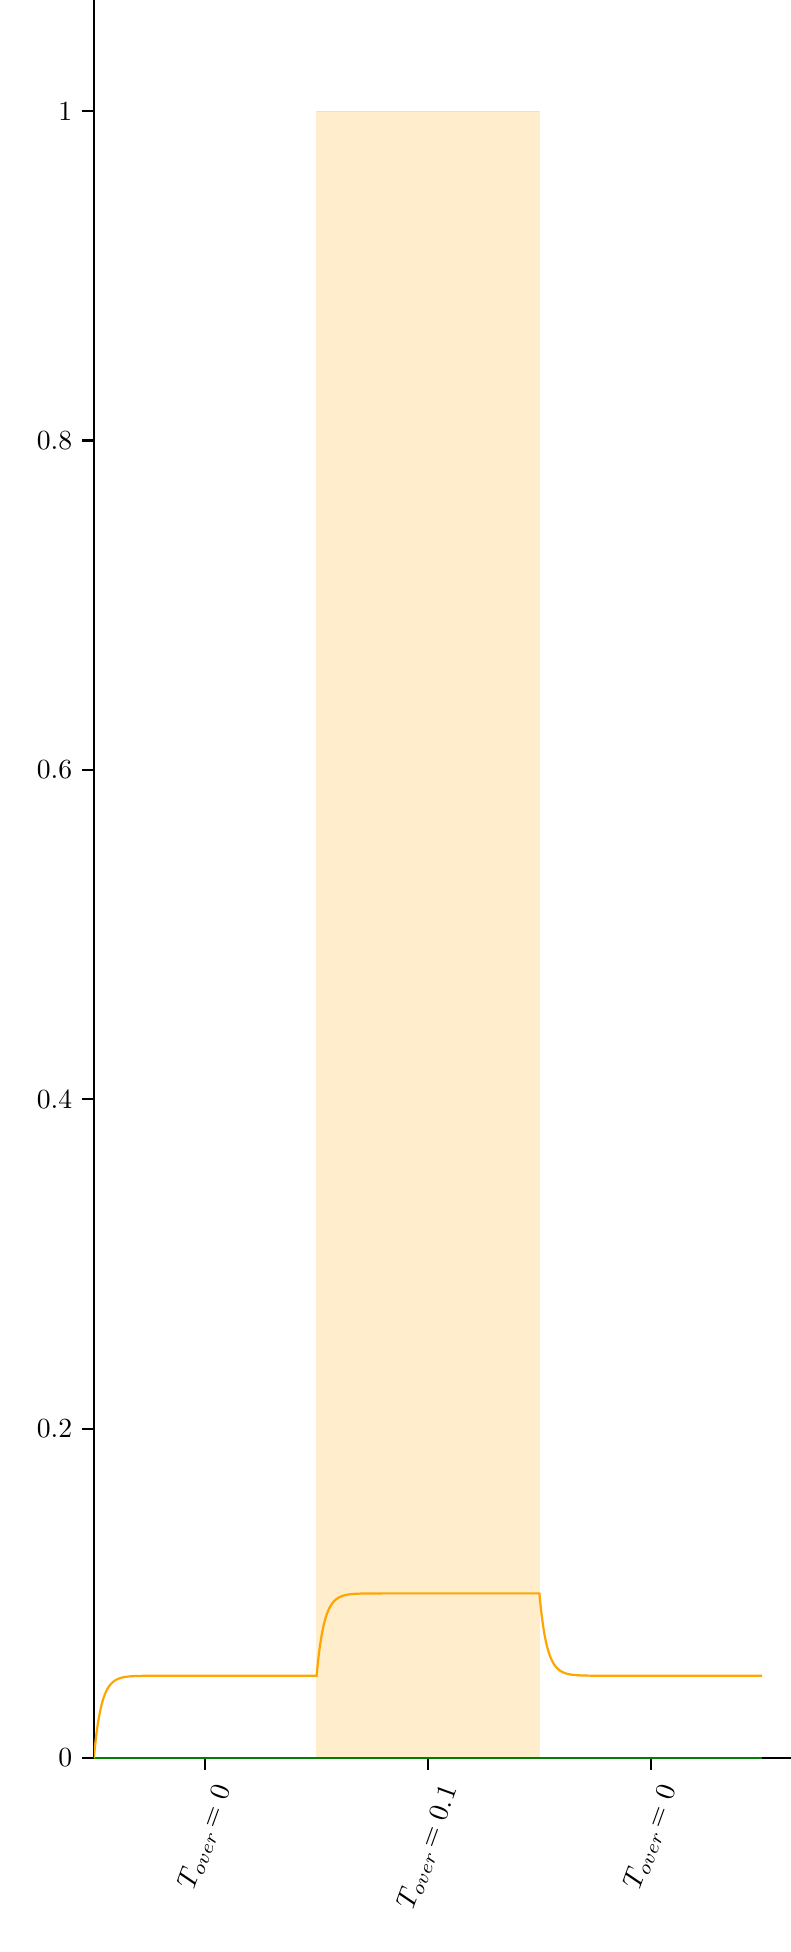
\begin{tikzpicture}[baseline]

\definecolor{darkgray176}{RGB}{176,176,176}
\definecolor{green}{RGB}{0,128,0}
\definecolor{lightgray204}{RGB}{204,204,204}
\definecolor{orange}{RGB}{255,165,0}

\begin{axis}[
 ytick={0,0.2,0.4,0.6,0.8,1},
 x tick label style = {rotate=70},
 y post scale=3, 
 transpose legend,
legend cell align={left},
legend style={fill opacity=0.8, draw opacity=1, text opacity=1, draw=lightgray204, anchor=south west,
    legend columns=4,
    /tikz/every even column/.append style={column sep=1.0cm},, at={(axis cs:5,1.1)}},
tick align=outside,
tick pos=left,
x grid style={darkgray176},
xmin=0, xmax=90,
xtick style={color=black},
xtick={15,45,75},
xticklabels={
  \(\displaystyle T_\text{over}\!=0\),
  \(\displaystyle T_\text{over}\!=0.1\),
  \(\displaystyle T_\text{over}\!=0\)
},
y grid style={darkgray176},
ymin=0, ymax=1.05,
ytick style={color=black}
]
\path [draw=orange, fill=orange, opacity=0.2]
(axis cs:30,0)
--(axis cs:30,1)
--(axis cs:60,1)
--(axis cs:60,0)
--cycle;

\addplot [thick, blue]
table {%
0 0
0.0001 0
0.0011 0
0.0111 0
0.1111 0
0.2111 0
0.3111 0
0.4111 0
0.5111 0
0.6111 0
0.7111 0
0.8111 0
0.9111 0
1.0111 0
1.1111 0
1.2111 0
1.3111 0
1.4111 0
1.5111 0
1.6111 0
1.7111 0
1.8111 0
1.9111 0
2.0111 0
2.1111 0
2.2111 0
2.3111 0
2.4111 0
2.5111 0
2.6111 0
2.7111 0
2.8111 0
2.9111 0
3.0111 0
3.1111 0
3.2111 0
3.3111 0
3.4111 0
3.5111 0
3.6111 0
3.7111 0
3.8111 0
3.9111 0
4.0111 0
4.1111 0
4.2111 0
4.3111 0
4.4111 0
4.5111 0
4.6111 0
4.7111 0
4.8111 0
4.9111 0
5.0111 0
5.1111 0
5.2111 0
5.3111 0
5.4111 0
5.5111 0
5.6111 0
5.7111 0
5.8111 0
5.9111 0
6.0111 0
6.1111 0
6.21109999999999 0
6.31109999999999 0
6.41109999999999 0
6.51109999999999 0
6.61109999999999 0
6.71109999999999 0
6.81109999999999 0
6.91109999999999 0
7.01109999999999 0
7.11109999999999 0
7.21109999999999 0
7.31109999999999 0
7.41109999999999 0
7.51109999999999 0
7.61109999999999 0
7.71109999999999 0
7.81109999999999 0
7.91109999999999 0
8.01109999999999 0
8.11109999999999 0
8.21109999999999 0
8.31109999999999 0
8.41109999999999 0
8.51109999999999 0
8.61109999999999 0
8.71109999999999 0
8.81109999999999 0
8.91109999999999 0
9.01109999999998 0
9.11109999999998 0
9.21109999999998 0
9.31109999999998 0
9.41109999999998 0
9.51109999999998 0
9.61109999999998 0
9.71109999999998 0
9.81109999999998 0
9.91109999999998 0
10.0111 0
10.1111 0
10.2111 0
10.3111 0
10.4111 0
10.5111 0
10.6111 0
10.7111 0
10.8111 0
10.9111 0
11.0111 0
11.1111 0
11.2111 0
11.3111 0
11.4111 0
11.5111 0
11.6111 0
11.7111 0
11.8111 0
11.9111 0
12.0111 0
12.1111 0
12.2111 0
12.3111 0
12.4111 0
12.5111 0
12.6111 0
12.7111 0
12.8111 0
12.9111 0
13.0111 0
13.1111 0
13.2111 0
13.3111 0
13.4111 0
13.5111 0
13.6111 0
13.7111 0
13.8111 0
13.9111 0
14.0111 0
14.1111 0
14.2111 0
14.3111 0
14.4111 0
14.5111 0
14.6111 0
14.7111 0
14.8111 0
14.9111 0
15.0111 0
15.1111 0
15.2111 0
15.3111 0
15.4111 0
15.5111 0
15.6111 0
15.7111 0
15.8111 0
15.9111 0
16.0111 0
16.1111 0
16.2111 0
16.3111 0
16.4111 0
16.5111 0
16.6111 0
16.7111 0
16.8111 0
16.9111 0
17.0111 0
17.1111 0
17.2111 0
17.3111 0
17.4111 0
17.5111 0
17.6111 0
17.7111 0
17.8111 0
17.9111 0
18.0111 0
18.1111 0
18.2111 0
18.3111 0
18.4111 0
18.5111 0
18.6111 0
18.7111 0
18.8111 0
18.9111 0
19.0111 0
19.1111 0
19.2111 0
19.3111 0
19.4111 0
19.5111 0
19.6111 0
19.7111 0
19.8111 0
19.9111 0
20.0111 0
20.1111 0
20.2111 0
20.3111 0
20.4111 0
20.5111 0
20.6111 0
20.7111 0
20.8111 0
20.9111 0
21.0111 0
21.1111 0
21.2111 0
21.3111 0
21.4111 0
21.5111 0
21.6111 0
21.7111 0
21.8111 0
21.9111 0
22.0111 0
22.1111 0
22.2111 0
22.3111 0
22.4111000000001 0
22.5111000000001 0
22.6111000000001 0
22.7111000000001 0
22.8111000000001 0
22.9111000000001 0
23.0111000000001 0
23.1111000000001 0
23.2111000000001 0
23.3111000000001 0
23.4111000000001 0
23.5111000000001 0
23.6111000000001 0
23.7111000000001 0
23.8111000000001 0
23.9111000000001 0
24.0111000000001 0
24.1111000000001 0
24.2111000000001 0
24.3111000000001 0
24.4111000000001 0
24.5111000000001 0
24.6111000000001 0
24.7111000000001 0
24.8111000000001 0
24.9111000000001 0
25.0111000000001 0
25.1111000000001 0
25.2111000000001 0
25.3111000000001 0
25.4111000000001 0
25.5111000000001 0
25.6111000000001 0
25.7111000000001 0
25.8111000000001 0
25.9111000000001 0
26.0111000000001 0
26.1111000000001 0
26.2111000000001 0
26.3111000000001 0
26.4111000000001 0
26.5111000000001 0
26.6111000000001 0
26.7111000000001 0
26.8111000000001 0
26.9111000000001 0
27.0111000000001 0
27.1111000000001 0
27.2111000000001 0
27.3111000000001 0
27.4111000000001 0
27.5111000000001 0
27.6111000000001 0
27.7111000000001 0
27.8111000000001 0
27.9111000000001 0
28.0111000000001 0
28.1111000000001 0
28.2111000000001 0
28.3111000000001 0
28.4111000000001 0
28.5111000000001 0
28.6111000000001 0
28.7111000000001 0
28.8111000000001 0
28.9111000000001 0
29.0111000000001 0
29.1111000000001 0
29.2111000000001 0
29.3111000000001 0
29.4111000000002 0
29.5111000000002 0
29.6111000000002 0
29.7111000000002 0
29.8111000000002 0
29.9111000000002 0
30 0
30 0
30.1 0
30.2 0
30.3 0
30.4 0
30.5 0
30.6 0
30.7 0
30.8 0
30.9 0
31 0
31.1 0
31.2 0
31.3 0
31.4 0
31.5 0
31.6 0
31.7 0
31.8 0
31.9 0
32 0
32.1 0
32.2 0
32.3 0
32.4 0
32.5 0
32.6 0
32.7 0
32.8 0
32.9 0
33 0
33.1 0
33.2 0
33.3 0
33.4 0
33.5 0
33.6000000000001 0
33.7000000000001 0
33.8000000000001 0
33.9000000000001 0
34.0000000000001 0
34.1000000000001 0
34.2000000000001 0
34.3000000000001 0
34.4000000000001 0
34.5000000000001 0
34.6000000000001 0
34.7000000000001 0
34.8000000000001 0
34.9000000000001 0
35.0000000000001 0
35.1000000000001 0
35.2000000000001 0
35.3000000000001 0
35.4000000000001 0
35.5000000000001 0
35.6000000000001 0
35.7000000000001 0
35.8000000000001 0
35.9000000000001 0
36.0000000000001 0
36.1000000000001 0
36.2000000000001 0
36.3000000000001 0
36.4000000000001 0
36.5000000000001 0
36.6000000000001 0
36.7000000000001 0
36.8000000000001 0
36.9000000000001 0
37.0000000000001 0
37.1000000000001 0
37.2000000000001 0
37.3000000000001 0
37.4000000000001 0
37.5000000000001 0
37.6000000000001 0
37.7000000000001 0
37.8000000000001 0
37.9000000000001 0
38.0000000000001 0
38.1000000000001 0
38.2000000000001 0
38.3000000000001 0
38.4000000000001 0
38.5000000000001 0
38.6000000000001 0
38.7000000000001 0
38.8000000000001 0
38.9000000000001 0
39.0000000000001 0
39.1000000000001 0
39.2000000000001 0
39.3000000000001 0
39.4000000000001 0
39.5000000000001 0
39.6000000000001 0
39.7000000000001 0
39.8000000000001 0
39.9000000000001 0
40.0000000000001 0
40.1000000000001 0
40.2000000000001 0
40.3000000000001 0
40.4000000000001 0
40.5000000000001 0
40.6000000000002 0
40.7000000000002 0
40.8000000000002 0
40.9000000000002 0
41.0000000000002 0
41.1000000000002 0
41.2000000000002 0
41.3000000000002 0
41.4000000000002 0
41.5000000000002 0
41.6000000000002 0
41.7000000000002 0
41.8000000000002 0
41.9000000000002 0
42.0000000000002 0
42.1000000000002 0
42.2000000000002 0
42.3000000000002 0
42.4000000000002 0
42.5000000000002 0
42.6000000000002 0
42.7000000000002 0
42.8000000000002 0
42.9000000000002 0
43.0000000000002 0
43.1000000000002 0
43.2000000000002 0
43.3000000000002 0
43.4000000000002 0
43.5000000000002 0
43.6000000000002 0
43.7000000000002 0
43.8000000000002 0
43.9000000000002 0
44.0000000000002 0
44.1000000000002 0
44.2000000000002 0
44.3000000000002 0
44.4000000000002 0
44.5000000000002 0
44.6000000000002 0
44.7000000000002 0
44.8000000000002 0
44.9000000000002 0
45.0000000000002 0
45.1000000000002 0
45.2000000000002 0
45.3000000000002 0
45.4000000000002 0
45.5000000000002 0
45.6000000000002 0
45.7000000000002 0
45.8000000000002 0
45.9000000000002 0
46.0000000000002 0
46.1000000000002 0
46.2000000000002 0
46.3000000000002 0
46.4000000000002 0
46.5000000000002 0
46.6000000000002 0
46.7000000000002 0
46.8000000000002 0
46.9000000000002 0
47.0000000000002 0
47.1000000000002 0
47.2000000000002 0
47.3000000000002 0
47.4000000000002 0
47.5000000000002 0
47.6000000000003 0
47.7000000000003 0
47.8000000000003 0
47.9000000000003 0
48.0000000000003 0
48.1000000000003 0
48.2000000000003 0
48.3000000000003 0
48.4000000000003 0
48.5000000000003 0
48.6000000000003 0
48.7000000000003 0
48.8000000000003 0
48.9000000000003 0
49.0000000000003 0
49.1000000000003 0
49.2000000000003 0
49.3000000000003 0
49.4000000000003 0
49.5000000000003 0
49.6000000000003 0
49.7000000000003 0
49.8000000000003 0
49.9000000000003 0
50.0000000000003 0
50.1000000000003 0
50.2000000000003 0
50.3000000000003 0
50.4000000000003 0
50.5000000000003 0
50.6000000000003 0
50.7000000000003 0
50.8000000000003 0
50.9000000000003 0
51.0000000000003 0
51.1000000000003 0
51.2000000000003 0
51.3000000000003 0
51.4000000000003 0
51.5000000000003 0
51.6000000000003 0
51.7000000000003 0
51.8000000000003 0
51.9000000000003 0
52.0000000000003 0
52.1000000000003 0
52.2000000000003 0
52.3000000000003 0
52.4000000000003 0
52.5000000000003 0
52.6000000000003 0
52.7000000000003 0
52.8000000000003 0
52.9000000000003 0
53.0000000000003 0
53.1000000000003 0
53.2000000000003 0
53.3000000000003 0
53.4000000000003 0
53.5000000000003 0
53.6000000000003 0
53.7000000000003 0
53.8000000000003 0
53.9000000000003 0
54.0000000000003 0
54.1000000000003 0
54.2000000000003 0
54.3000000000003 0
54.4000000000003 0
54.5000000000003 0
54.6000000000003 0
54.7000000000004 0
54.8000000000004 0
54.9000000000004 0
55.0000000000004 0
55.1000000000004 0
55.2000000000004 0
55.3000000000004 0
55.4000000000004 0
55.5000000000004 0
55.6000000000004 0
55.7000000000004 0
55.8000000000004 0
55.9000000000004 0
56.0000000000004 0
56.1000000000004 0
56.2000000000004 0
56.3000000000004 0
56.4000000000004 0
56.5000000000004 0
56.6000000000004 0
56.7000000000004 0
56.8000000000004 0
56.9000000000004 0
57.0000000000004 0
57.1000000000004 0
57.2000000000004 0
57.3000000000004 0
57.4000000000004 0
57.5000000000004 0
57.6000000000004 0
57.7000000000004 0
57.8000000000004 0
57.9000000000004 0
58.0000000000004 0
58.1000000000004 0
58.2000000000004 0
58.3000000000004 0
58.4000000000004 0
58.5000000000004 0
58.6000000000004 0
58.7000000000004 0
58.8000000000004 0
58.9000000000004 0
59.0000000000004 0
59.1000000000004 0
59.2000000000004 0
59.3000000000004 0
59.4000000000004 0
59.5000000000004 0
59.6000000000004 0
59.7000000000004 0
59.8000000000004 0
59.9000000000004 0
60 0
60 0
60.1 0
60.2 0
60.3 0
60.4 0
60.5 0
60.6 0
60.7 0
60.8 0
60.9 0
61 0
61.1 0
61.2 0
61.3 0
61.4 0
61.5 0
61.6 0
61.7 0
61.8 0
61.9 0
62 0
62.1 0
62.2 0
62.3 0
62.4 0
62.5 0
62.6 0
62.7 0
62.8 0
62.9 0
63 0
63.1 0
63.2 0
63.3 0
63.4 0
63.5 0
63.6000000000001 0
63.7000000000001 0
63.8000000000001 0
63.9000000000001 0
64.0000000000001 0
64.1000000000001 0
64.2 0
64.3 0
64.4 0
64.5 0
64.6 0
64.7 0
64.8 0
64.9 0
65 0
65.1 0
65.2 0
65.3 0
65.4 0
65.5 0
65.6 0
65.7 0
65.8 0
65.8999999999999 0
65.9999999999999 0
66.0999999999999 0
66.1999999999999 0
66.2999999999999 0
66.3999999999999 0
66.4999999999999 0
66.5999999999999 0
66.6999999999999 0
66.7999999999999 0
66.8999999999999 0
66.9999999999999 0
67.0999999999999 0
67.1999999999999 0
67.2999999999999 0
67.3999999999999 0
67.4999999999999 0
67.5999999999999 0
67.6999999999998 0
67.7999999999998 0
67.8999999999998 0
67.9999999999998 0
68.0999999999998 0
68.1999999999998 0
68.2999999999998 0
68.3999999999998 0
68.4999999999998 0
68.5999999999998 0
68.6999999999998 0
68.7999999999998 0
68.8999999999998 0
68.9999999999998 0
69.0999999999998 0
69.1999999999998 0
69.2999999999998 0
69.3999999999997 0
69.4999999999997 0
69.5999999999997 0
69.6999999999997 0
69.7999999999997 0
69.8999999999997 0
69.9999999999997 0
70.0999999999997 0
70.1999999999997 0
70.2999999999997 0
70.3999999999997 0
70.4999999999997 0
70.5999999999997 0
70.6999999999997 0
70.7999999999997 0
70.8999999999997 0
70.9999999999997 0
71.0999999999997 0
71.1999999999996 0
71.2999999999996 0
71.3999999999996 0
71.4999999999996 0
71.5999999999996 0
71.6999999999996 0
71.7999999999996 0
71.8999999999996 0
71.9999999999996 0
72.0999999999996 0
72.1999999999996 0
72.2999999999996 0
72.3999999999996 0
72.4999999999996 0
72.5999999999996 0
72.6999999999996 0
72.7999999999996 0
72.8999999999996 0
72.9999999999995 0
73.0999999999995 0
73.1999999999995 0
73.2999999999995 0
73.3999999999995 0
73.4999999999995 0
73.5999999999995 0
73.6999999999995 0
73.7999999999995 0
73.8999999999995 0
73.9999999999995 0
74.0999999999995 0
74.1999999999995 0
74.2999999999995 0
74.3999999999995 0
74.4999999999995 0
74.5999999999995 0
74.6999999999994 0
74.7999999999994 0
74.8999999999994 0
74.9999999999994 0
75.0999999999994 0
75.1999999999994 0
75.2999999999994 0
75.3999999999994 0
75.4999999999994 0
75.5999999999994 0
75.6999999999994 0
75.7999999999994 0
75.8999999999994 0
75.9999999999994 0
76.0999999999994 0
76.1999999999994 0
76.2999999999994 0
76.3999999999994 0
76.4999999999993 0
76.5999999999993 0
76.6999999999993 0
76.7999999999993 0
76.8999999999993 0
76.9999999999993 0
77.0999999999993 0
77.1999999999993 0
77.2999999999993 0
77.3999999999993 0
77.4999999999993 0
77.5999999999993 0
77.6999999999993 0
77.7999999999993 0
77.8999999999993 0
77.9999999999993 0
78.0999999999993 0
78.1999999999992 0
78.2999999999992 0
78.3999999999992 0
78.4999999999992 0
78.5999999999992 0
78.6999999999992 0
78.7999999999992 0
78.8999999999992 0
78.9999999999992 0
79.0999999999992 0
79.1999999999992 0
79.2999999999992 0
79.3999999999992 0
79.4999999999992 0
79.5999999999992 0
79.6999999999992 0
79.7999999999992 0
79.8999999999992 0
79.9999999999991 0
80.0999999999991 0
80.1999999999991 0
80.2999999999991 0
80.3999999999991 0
80.4999999999991 0
80.5999999999991 0
80.6999999999991 0
80.7999999999991 0
80.8999999999991 0
80.9999999999991 0
81.0999999999991 0
81.1999999999991 0
81.2999999999991 0
81.3999999999991 0
81.4999999999991 0
81.5999999999991 0
81.6999999999991 0
81.799999999999 0
81.899999999999 0
81.999999999999 0
82.099999999999 0
82.199999999999 0
82.299999999999 0
82.399999999999 0
82.499999999999 0
82.599999999999 0
82.699999999999 0
82.799999999999 0
82.899999999999 0
82.999999999999 0
83.099999999999 0
83.199999999999 0
83.299999999999 0
83.399999999999 0
83.4999999999989 0
83.5999999999989 0
83.6999999999989 0
83.7999999999989 0
83.8999999999989 0
83.9999999999989 0
84.0999999999989 0
84.1999999999989 0
84.2999999999989 0
84.3999999999989 0
84.4999999999989 0
84.5999999999989 0
84.6999999999989 0
84.7999999999989 0
84.8999999999989 0
84.9999999999989 0
85.0999999999989 0
85.1999999999989 0
85.2999999999988 0
85.3999999999988 0
85.4999999999988 0
85.5999999999988 0
85.6999999999988 0
85.7999999999988 0
85.8999999999988 0
85.9999999999988 0
86.0999999999988 0
86.1999999999988 0
86.2999999999988 0
86.3999999999988 0
86.4999999999988 0
86.5999999999988 0
86.6999999999988 0
86.7999999999988 0
86.8999999999988 0
86.9999999999987 0
87.0999999999987 0
87.1999999999987 0
87.2999999999987 0
87.3999999999987 0
87.4999999999987 0
87.5999999999987 0
87.6999999999987 0
87.7999999999987 0
87.8999999999987 0
87.9999999999987 0
88.0999999999987 0
88.1999999999987 0
88.2999999999987 0
88.3999999999987 0
88.4999999999987 0
88.5999999999987 0
88.6999999999987 0
88.7999999999986 0
88.8999999999986 0
88.9999999999986 0
89.0999999999986 0
89.1999999999986 0
89.2999999999986 0
89.3999999999986 0
89.4999999999986 0
89.5999999999986 0
89.6999999999986 0
89.7999999999986 0
89.8999999999986 0
89.9999999999986 0
90 0
};
\addplot [thick, green]
table {%
0 0
0.0001 0
0.0011 0
0.0111 0
0.1111 0
0.2111 0
0.3111 0
0.4111 0
0.5111 0
0.6111 0
0.7111 0
0.8111 0
0.9111 0
1.0111 0
1.1111 0
1.2111 0
1.3111 0
1.4111 0
1.5111 0
1.6111 0
1.7111 0
1.8111 0
1.9111 0
2.0111 0
2.1111 0
2.2111 0
2.3111 0
2.4111 0
2.5111 0
2.6111 0
2.7111 0
2.8111 0
2.9111 0
3.0111 0
3.1111 0
3.2111 0
3.3111 0
3.4111 0
3.5111 0
3.6111 0
3.7111 0
3.8111 0
3.9111 0
4.0111 0
4.1111 0
4.2111 0
4.3111 0
4.4111 0
4.5111 0
4.6111 0
4.7111 0
4.8111 0
4.9111 0
5.0111 0
5.1111 0
5.2111 0
5.3111 0
5.4111 0
5.5111 0
5.6111 0
5.7111 0
5.8111 0
5.9111 0
6.0111 0
6.1111 0
6.21109999999999 0
6.31109999999999 0
6.41109999999999 0
6.51109999999999 0
6.61109999999999 0
6.71109999999999 0
6.81109999999999 0
6.91109999999999 0
7.01109999999999 0
7.11109999999999 0
7.21109999999999 0
7.31109999999999 0
7.41109999999999 0
7.51109999999999 0
7.61109999999999 0
7.71109999999999 0
7.81109999999999 0
7.91109999999999 0
8.01109999999999 0
8.11109999999999 0
8.21109999999999 0
8.31109999999999 0
8.41109999999999 0
8.51109999999999 0
8.61109999999999 0
8.71109999999999 0
8.81109999999999 0
8.91109999999999 0
9.01109999999998 0
9.11109999999998 0
9.21109999999998 0
9.31109999999998 0
9.41109999999998 0
9.51109999999998 0
9.61109999999998 0
9.71109999999998 0
9.81109999999998 0
9.91109999999998 0
10.0111 0
10.1111 0
10.2111 0
10.3111 0
10.4111 0
10.5111 0
10.6111 0
10.7111 0
10.8111 0
10.9111 0
11.0111 0
11.1111 0
11.2111 0
11.3111 0
11.4111 0
11.5111 0
11.6111 0
11.7111 0
11.8111 0
11.9111 0
12.0111 0
12.1111 0
12.2111 0
12.3111 0
12.4111 0
12.5111 0
12.6111 0
12.7111 0
12.8111 0
12.9111 0
13.0111 0
13.1111 0
13.2111 0
13.3111 0
13.4111 0
13.5111 0
13.6111 0
13.7111 0
13.8111 0
13.9111 0
14.0111 0
14.1111 0
14.2111 0
14.3111 0
14.4111 0
14.5111 0
14.6111 0
14.7111 0
14.8111 0
14.9111 0
15.0111 0
15.1111 0
15.2111 0
15.3111 0
15.4111 0
15.5111 0
15.6111 0
15.7111 0
15.8111 0
15.9111 0
16.0111 0
16.1111 0
16.2111 0
16.3111 0
16.4111 0
16.5111 0
16.6111 0
16.7111 0
16.8111 0
16.9111 0
17.0111 0
17.1111 0
17.2111 0
17.3111 0
17.4111 0
17.5111 0
17.6111 0
17.7111 0
17.8111 0
17.9111 0
18.0111 0
18.1111 0
18.2111 0
18.3111 0
18.4111 0
18.5111 0
18.6111 0
18.7111 0
18.8111 0
18.9111 0
19.0111 0
19.1111 0
19.2111 0
19.3111 0
19.4111 0
19.5111 0
19.6111 0
19.7111 0
19.8111 0
19.9111 0
20.0111 0
20.1111 0
20.2111 0
20.3111 0
20.4111 0
20.5111 0
20.6111 0
20.7111 0
20.8111 0
20.9111 0
21.0111 0
21.1111 0
21.2111 0
21.3111 0
21.4111 0
21.5111 0
21.6111 0
21.7111 0
21.8111 0
21.9111 0
22.0111 0
22.1111 0
22.2111 0
22.3111 0
22.4111000000001 0
22.5111000000001 0
22.6111000000001 0
22.7111000000001 0
22.8111000000001 0
22.9111000000001 0
23.0111000000001 0
23.1111000000001 0
23.2111000000001 0
23.3111000000001 0
23.4111000000001 0
23.5111000000001 0
23.6111000000001 0
23.7111000000001 0
23.8111000000001 0
23.9111000000001 0
24.0111000000001 0
24.1111000000001 0
24.2111000000001 0
24.3111000000001 0
24.4111000000001 0
24.5111000000001 0
24.6111000000001 0
24.7111000000001 0
24.8111000000001 0
24.9111000000001 0
25.0111000000001 0
25.1111000000001 0
25.2111000000001 0
25.3111000000001 0
25.4111000000001 0
25.5111000000001 0
25.6111000000001 0
25.7111000000001 0
25.8111000000001 0
25.9111000000001 0
26.0111000000001 0
26.1111000000001 0
26.2111000000001 0
26.3111000000001 0
26.4111000000001 0
26.5111000000001 0
26.6111000000001 0
26.7111000000001 0
26.8111000000001 0
26.9111000000001 0
27.0111000000001 0
27.1111000000001 0
27.2111000000001 0
27.3111000000001 0
27.4111000000001 0
27.5111000000001 0
27.6111000000001 0
27.7111000000001 0
27.8111000000001 0
27.9111000000001 0
28.0111000000001 0
28.1111000000001 0
28.2111000000001 0
28.3111000000001 0
28.4111000000001 0
28.5111000000001 0
28.6111000000001 0
28.7111000000001 0
28.8111000000001 0
28.9111000000001 0
29.0111000000001 0
29.1111000000001 0
29.2111000000001 0
29.3111000000001 0
29.4111000000002 0
29.5111000000002 0
29.6111000000002 0
29.7111000000002 0
29.8111000000002 0
29.9111000000002 0
30 0
30 0
30.1 0
30.2 0
30.3 0
30.4 0
30.5 0
30.6 0
30.7 0
30.8 0
30.9 0
31 0
31.1 0
31.2 0
31.3 0
31.4 0
31.5 0
31.6 0
31.7 0
31.8 0
31.9 0
32 0
32.1 0
32.2 0
32.3 0
32.4 0
32.5 0
32.6 0
32.7 0
32.8 0
32.9 0
33 0
33.1 0
33.2 0
33.3 0
33.4 0
33.5 0
33.6000000000001 0
33.7000000000001 0
33.8000000000001 0
33.9000000000001 0
34.0000000000001 0
34.1000000000001 0
34.2000000000001 0
34.3000000000001 0
34.4000000000001 0
34.5000000000001 0
34.6000000000001 0
34.7000000000001 0
34.8000000000001 0
34.9000000000001 0
35.0000000000001 0
35.1000000000001 0
35.2000000000001 0
35.3000000000001 0
35.4000000000001 0
35.5000000000001 0
35.6000000000001 0
35.7000000000001 0
35.8000000000001 0
35.9000000000001 0
36.0000000000001 0
36.1000000000001 0
36.2000000000001 0
36.3000000000001 0
36.4000000000001 0
36.5000000000001 0
36.6000000000001 0
36.7000000000001 0
36.8000000000001 0
36.9000000000001 0
37.0000000000001 0
37.1000000000001 0
37.2000000000001 0
37.3000000000001 0
37.4000000000001 0
37.5000000000001 0
37.6000000000001 0
37.7000000000001 0
37.8000000000001 0
37.9000000000001 0
38.0000000000001 0
38.1000000000001 0
38.2000000000001 0
38.3000000000001 0
38.4000000000001 0
38.5000000000001 0
38.6000000000001 0
38.7000000000001 0
38.8000000000001 0
38.9000000000001 0
39.0000000000001 0
39.1000000000001 0
39.2000000000001 0
39.3000000000001 0
39.4000000000001 0
39.5000000000001 0
39.6000000000001 0
39.7000000000001 0
39.8000000000001 0
39.9000000000001 0
40.0000000000001 0
40.1000000000001 0
40.2000000000001 0
40.3000000000001 0
40.4000000000001 0
40.5000000000001 0
40.6000000000002 0
40.7000000000002 0
40.8000000000002 0
40.9000000000002 0
41.0000000000002 0
41.1000000000002 0
41.2000000000002 0
41.3000000000002 0
41.4000000000002 0
41.5000000000002 0
41.6000000000002 0
41.7000000000002 0
41.8000000000002 0
41.9000000000002 0
42.0000000000002 0
42.1000000000002 0
42.2000000000002 0
42.3000000000002 0
42.4000000000002 0
42.5000000000002 0
42.6000000000002 0
42.7000000000002 0
42.8000000000002 0
42.9000000000002 0
43.0000000000002 0
43.1000000000002 0
43.2000000000002 0
43.3000000000002 0
43.4000000000002 0
43.5000000000002 0
43.6000000000002 0
43.7000000000002 0
43.8000000000002 0
43.9000000000002 0
44.0000000000002 0
44.1000000000002 0
44.2000000000002 0
44.3000000000002 0
44.4000000000002 0
44.5000000000002 0
44.6000000000002 0
44.7000000000002 0
44.8000000000002 0
44.9000000000002 0
45.0000000000002 0
45.1000000000002 0
45.2000000000002 0
45.3000000000002 0
45.4000000000002 0
45.5000000000002 0
45.6000000000002 0
45.7000000000002 0
45.8000000000002 0
45.9000000000002 0
46.0000000000002 0
46.1000000000002 0
46.2000000000002 0
46.3000000000002 0
46.4000000000002 0
46.5000000000002 0
46.6000000000002 0
46.7000000000002 0
46.8000000000002 0
46.9000000000002 0
47.0000000000002 0
47.1000000000002 0
47.2000000000002 0
47.3000000000002 0
47.4000000000002 0
47.5000000000002 0
47.6000000000003 0
47.7000000000003 0
47.8000000000003 0
47.9000000000003 0
48.0000000000003 0
48.1000000000003 0
48.2000000000003 0
48.3000000000003 0
48.4000000000003 0
48.5000000000003 0
48.6000000000003 0
48.7000000000003 0
48.8000000000003 0
48.9000000000003 0
49.0000000000003 0
49.1000000000003 0
49.2000000000003 0
49.3000000000003 0
49.4000000000003 0
49.5000000000003 0
49.6000000000003 0
49.7000000000003 0
49.8000000000003 0
49.9000000000003 0
50.0000000000003 0
50.1000000000003 0
50.2000000000003 0
50.3000000000003 0
50.4000000000003 0
50.5000000000003 0
50.6000000000003 0
50.7000000000003 0
50.8000000000003 0
50.9000000000003 0
51.0000000000003 0
51.1000000000003 0
51.2000000000003 0
51.3000000000003 0
51.4000000000003 0
51.5000000000003 0
51.6000000000003 0
51.7000000000003 0
51.8000000000003 0
51.9000000000003 0
52.0000000000003 0
52.1000000000003 0
52.2000000000003 0
52.3000000000003 0
52.4000000000003 0
52.5000000000003 0
52.6000000000003 0
52.7000000000003 0
52.8000000000003 0
52.9000000000003 0
53.0000000000003 0
53.1000000000003 0
53.2000000000003 0
53.3000000000003 0
53.4000000000003 0
53.5000000000003 0
53.6000000000003 0
53.7000000000003 0
53.8000000000003 0
53.9000000000003 0
54.0000000000003 0
54.1000000000003 0
54.2000000000003 0
54.3000000000003 0
54.4000000000003 0
54.5000000000003 0
54.6000000000003 0
54.7000000000004 0
54.8000000000004 0
54.9000000000004 0
55.0000000000004 0
55.1000000000004 0
55.2000000000004 0
55.3000000000004 0
55.4000000000004 0
55.5000000000004 0
55.6000000000004 0
55.7000000000004 0
55.8000000000004 0
55.9000000000004 0
56.0000000000004 0
56.1000000000004 0
56.2000000000004 0
56.3000000000004 0
56.4000000000004 0
56.5000000000004 0
56.6000000000004 0
56.7000000000004 0
56.8000000000004 0
56.9000000000004 0
57.0000000000004 0
57.1000000000004 0
57.2000000000004 0
57.3000000000004 0
57.4000000000004 0
57.5000000000004 0
57.6000000000004 0
57.7000000000004 0
57.8000000000004 0
57.9000000000004 0
58.0000000000004 0
58.1000000000004 0
58.2000000000004 0
58.3000000000004 0
58.4000000000004 0
58.5000000000004 0
58.6000000000004 0
58.7000000000004 0
58.8000000000004 0
58.9000000000004 0
59.0000000000004 0
59.1000000000004 0
59.2000000000004 0
59.3000000000004 0
59.4000000000004 0
59.5000000000004 0
59.6000000000004 0
59.7000000000004 0
59.8000000000004 0
59.9000000000004 0
60 0
60 0
60.1 0
60.2 0
60.3 0
60.4 0
60.5 0
60.6 0
60.7 0
60.8 0
60.9 0
61 0
61.1 0
61.2 0
61.3 0
61.4 0
61.5 0
61.6 0
61.7 0
61.8 0
61.9 0
62 0
62.1 0
62.2 0
62.3 0
62.4 0
62.5 0
62.6 0
62.7 0
62.8 0
62.9 0
63 0
63.1 0
63.2 0
63.3 0
63.4 0
63.5 0
63.6000000000001 0
63.7000000000001 0
63.8000000000001 0
63.9000000000001 0
64.0000000000001 0
64.1000000000001 0
64.2 0
64.3 0
64.4 0
64.5 0
64.6 0
64.7 0
64.8 0
64.9 0
65 0
65.1 0
65.2 0
65.3 0
65.4 0
65.5 0
65.6 0
65.7 0
65.8 0
65.8999999999999 0
65.9999999999999 0
66.0999999999999 0
66.1999999999999 0
66.2999999999999 0
66.3999999999999 0
66.4999999999999 0
66.5999999999999 0
66.6999999999999 0
66.7999999999999 0
66.8999999999999 0
66.9999999999999 0
67.0999999999999 0
67.1999999999999 0
67.2999999999999 0
67.3999999999999 0
67.4999999999999 0
67.5999999999999 0
67.6999999999998 0
67.7999999999998 0
67.8999999999998 0
67.9999999999998 0
68.0999999999998 0
68.1999999999998 0
68.2999999999998 0
68.3999999999998 0
68.4999999999998 0
68.5999999999998 0
68.6999999999998 0
68.7999999999998 0
68.8999999999998 0
68.9999999999998 0
69.0999999999998 0
69.1999999999998 0
69.2999999999998 0
69.3999999999997 0
69.4999999999997 0
69.5999999999997 0
69.6999999999997 0
69.7999999999997 0
69.8999999999997 0
69.9999999999997 0
70.0999999999997 0
70.1999999999997 0
70.2999999999997 0
70.3999999999997 0
70.4999999999997 0
70.5999999999997 0
70.6999999999997 0
70.7999999999997 0
70.8999999999997 0
70.9999999999997 0
71.0999999999997 0
71.1999999999996 0
71.2999999999996 0
71.3999999999996 0
71.4999999999996 0
71.5999999999996 0
71.6999999999996 0
71.7999999999996 0
71.8999999999996 0
71.9999999999996 0
72.0999999999996 0
72.1999999999996 0
72.2999999999996 0
72.3999999999996 0
72.4999999999996 0
72.5999999999996 0
72.6999999999996 0
72.7999999999996 0
72.8999999999996 0
72.9999999999995 0
73.0999999999995 0
73.1999999999995 0
73.2999999999995 0
73.3999999999995 0
73.4999999999995 0
73.5999999999995 0
73.6999999999995 0
73.7999999999995 0
73.8999999999995 0
73.9999999999995 0
74.0999999999995 0
74.1999999999995 0
74.2999999999995 0
74.3999999999995 0
74.4999999999995 0
74.5999999999995 0
74.6999999999994 0
74.7999999999994 0
74.8999999999994 0
74.9999999999994 0
75.0999999999994 0
75.1999999999994 0
75.2999999999994 0
75.3999999999994 0
75.4999999999994 0
75.5999999999994 0
75.6999999999994 0
75.7999999999994 0
75.8999999999994 0
75.9999999999994 0
76.0999999999994 0
76.1999999999994 0
76.2999999999994 0
76.3999999999994 0
76.4999999999993 0
76.5999999999993 0
76.6999999999993 0
76.7999999999993 0
76.8999999999993 0
76.9999999999993 0
77.0999999999993 0
77.1999999999993 0
77.2999999999993 0
77.3999999999993 0
77.4999999999993 0
77.5999999999993 0
77.6999999999993 0
77.7999999999993 0
77.8999999999993 0
77.9999999999993 0
78.0999999999993 0
78.1999999999992 0
78.2999999999992 0
78.3999999999992 0
78.4999999999992 0
78.5999999999992 0
78.6999999999992 0
78.7999999999992 0
78.8999999999992 0
78.9999999999992 0
79.0999999999992 0
79.1999999999992 0
79.2999999999992 0
79.3999999999992 0
79.4999999999992 0
79.5999999999992 0
79.6999999999992 0
79.7999999999992 0
79.8999999999992 0
79.9999999999991 0
80.0999999999991 0
80.1999999999991 0
80.2999999999991 0
80.3999999999991 0
80.4999999999991 0
80.5999999999991 0
80.6999999999991 0
80.7999999999991 0
80.8999999999991 0
80.9999999999991 0
81.0999999999991 0
81.1999999999991 0
81.2999999999991 0
81.3999999999991 0
81.4999999999991 0
81.5999999999991 0
81.6999999999991 0
81.799999999999 0
81.899999999999 0
81.999999999999 0
82.099999999999 0
82.199999999999 0
82.299999999999 0
82.399999999999 0
82.499999999999 0
82.599999999999 0
82.699999999999 0
82.799999999999 0
82.899999999999 0
82.999999999999 0
83.099999999999 0
83.199999999999 0
83.299999999999 0
83.399999999999 0
83.4999999999989 0
83.5999999999989 0
83.6999999999989 0
83.7999999999989 0
83.8999999999989 0
83.9999999999989 0
84.0999999999989 0
84.1999999999989 0
84.2999999999989 0
84.3999999999989 0
84.4999999999989 0
84.5999999999989 0
84.6999999999989 0
84.7999999999989 0
84.8999999999989 0
84.9999999999989 0
85.0999999999989 0
85.1999999999989 0
85.2999999999988 0
85.3999999999988 0
85.4999999999988 0
85.5999999999988 0
85.6999999999988 0
85.7999999999988 0
85.8999999999988 0
85.9999999999988 0
86.0999999999988 0
86.1999999999988 0
86.2999999999988 0
86.3999999999988 0
86.4999999999988 0
86.5999999999988 0
86.6999999999988 0
86.7999999999988 0
86.8999999999988 0
86.9999999999987 0
87.0999999999987 0
87.1999999999987 0
87.2999999999987 0
87.3999999999987 0
87.4999999999987 0
87.5999999999987 0
87.6999999999987 0
87.7999999999987 0
87.8999999999987 0
87.9999999999987 0
88.0999999999987 0
88.1999999999987 0
88.2999999999987 0
88.3999999999987 0
88.4999999999987 0
88.5999999999987 0
88.6999999999987 0
88.7999999999986 0
88.8999999999986 0
88.9999999999986 0
89.0999999999986 0
89.1999999999986 0
89.2999999999986 0
89.3999999999986 0
89.4999999999986 0
89.5999999999986 0
89.6999999999986 0
89.7999999999986 0
89.8999999999986 0
89.9999999999986 0
90 0
};
\addplot [thick, orange]
table {%
0 0
0.0001 4.99975000833312e-06
0.0011 5.49697610886171e-05
0.0111 0.0005519311153686
0.1111 0.0052575370088613
0.2111 0.00951534529722334
0.3111 0.0133679695566231
0.4111 0.0168539681453068
0.5111 0.020008230108605
0.6111 0.0228623243602227
0.7111 0.0254448156345365
0.8111 0.027781550372055
0.9111 0.0298959153992811
1.0111 0.0318090719919305
1.1111 0.0335401676640909
1.2111 0.0351065278029765
1.3111 0.036523829067226
1.4111 0.0378062562841701
1.5111 0.0389666444163501
1.6111 0.0400166070181366
1.7111 0.0409666524680836
1.8111 0.041826289140313
1.9111 0.0426041205675177
2.0111 0.0433079315480081
2.1111 0.0439447660585897
2.2111 0.0445209977530499
2.3111 0.0450423937518271
2.4111 0.0455141723612901
2.5111 0.0459410553003014
2.6111 0.046327314956767
2.7111 0.0466768171471296
2.8111 0.0469930598067591
2.9111 0.0472792079984652
3.0111 0.0475381255895092
3.1111 0.0477724039141506
3.2111 0.0479843877085906
3.3111 0.0481761985778802
3.4111 0.0483497562296565
3.5111 0.0485067976872217
3.6111 0.0486488946742563
3.7111 0.0487774693451577
3.8111 0.0488938085184391
3.9111 0.0489990765556421
4.0111 0.0490943270146579
4.1111 0.0491805131940888
4.2111 0.0492584976741811
4.3111 0.0493290609498179
4.4111 0.0493929092419742
4.5111 0.0494506815658139
4.6111 0.0495029561261681
4.7111 0.0495502561044036
4.8111 0.0495930548945974
4.9111 0.0496317808414241
5.0111 0.0496668215271733
5.1111 0.0496985276508032
5.2111 0.0497272165378539
5.3111 0.0497531753163477
5.4111 0.0497766637904631
5.5111 0.0497979170407423
5.6111 0.0498171477768561
5.7111 0.049834548466474
5.8111 0.049850293261545
5.9111 0.0498645397412693
6.0111 0.0498774304892033
6.1111 0.0498890945202844
6.21109999999999 0.0498996485720551
6.31109999999999 0.0499091982730123
6.41109999999999 0.0499178391997722
6.51109999999999 0.0499256578336337
6.61109999999999 0.0499327324261118
6.71109999999999 0.0499391337821054
6.81109999999999 0.0499449259685366
6.91109999999999 0.0499501669555534
7.01109999999999 0.0499549091967153
7.11109999999999 0.0499592001539653
7.21109999999999 0.0499630827726455
7.31109999999999 0.0499665959113086
7.41109999999999 0.0499697747306267
7.51109999999999 0.0499726510452918
7.61109999999999 0.0499752536424277
7.71109999999999 0.0499776085697011
7.81109999999999 0.0499797393960156
7.91109999999999 0.0499816674473969
8.01109999999999 0.0499834120204311
8.11109999999999 0.0499849905753915
8.21109999999999 0.0499864189109866
8.31109999999999 0.049987711322479
8.41109999999999 0.0499888807447571
8.51109999999999 0.0499899388817923
8.61109999999999 0.0499908963237754
8.71109999999999 0.0499917626531076
8.81109999999999 0.0499925465403039
8.91109999999999 0.049993255830771
9.01109999999998 0.049993897623326
9.11109999999998 0.0499944783412446
9.21109999999998 0.0499950037965468
9.31109999999998 0.049995479248166
9.41109999999998 0.0499959094545816
9.51109999999998 0.049996298721444
9.61109999999998 0.0499966509446669
9.71109999999998 0.0499969696494185
9.81109999999998 0.0499972580254032
9.91109999999998 0.0499975189587847
10.0111 0.049997755061072
10.1111 0.049997968695256
10.2111 0.0499981619994596
10.3111 0.0499983369083362
10.4111 0.0499984951724324
10.5111 0.0499986383757087
10.6111 0.0499987679513915
10.7111 0.0499988851963179
10.8111 0.0499989912839143
10.9111 0.0499990872759412
11.0111 0.049999174133119
11.1111 0.0499992527247435
11.2111 0.0499993238373861
11.3111 0.0499993881827661
11.4111 0.0499994464048736
11.5111 0.049999499086415
11.6111 0.0499995467546449
11.7111 0.0499995898866431
11.8111 0.0499996289140889
11.9111 0.0499996642275822
12.0111 0.0499996961805523
12.1111 0.0499997250927953
12.2111 0.0499997512536747
12.3111 0.0499997749250171
12.4111 0.0499997963437336
12.5111 0.0499998157241897
12.6111 0.0499998332603515
12.7111 0.0499998491277269
12.8111 0.0499998634851219
12.9111 0.0499998764762302
13.0111 0.049999888231071
13.1111 0.0499998988672909
13.2111 0.0499999084913405
13.3111 0.0499999171995408
13.4111 0.0499999250790463
13.5111 0.0499999322087177
13.6111 0.0499999386599111
13.7111 0.0499999444971923
13.8111 0.0499999497789828
13.9111 0.0499999545581444
14.0111 0.0499999588825087
14.1111 0.0499999627953554
14.2111 0.0499999663358454
14.3111 0.0499999695394132
14.4111 0.0499999724381213
14.5111 0.0499999750609809
14.6111 0.0499999774342423
14.7111 0.0499999795816581
14.8111 0.0499999815247202
14.9111 0.0499999832828755
15.0111 0.0499999848737202
15.1111 0.0499999863131761
15.2111 0.0499999876156496
15.3111 0.0499999887941763
15.4111 0.0499999898605514
15.5111 0.0499999908254475
15.6111 0.0499999916985216
15.7111 0.0499999924885118
15.8111 0.0499999932033244
15.9111 0.0499999938501136
16.0111 0.0499999944353526
16.1111 0.0499999949648988
16.2111 0.0499999954440521
16.3111 0.0499999958776078
16.4111 0.0499999962699053
16.5111 0.0499999966248708
16.6111 0.0499999969460568
16.7111 0.0499999972366779
16.8111 0.0499999974996428
16.9111 0.0499999977375832
17.0111 0.0499999979528806
17.1111 0.0499999981476898
17.2111 0.0499999983239604
17.3111 0.0499999984834567
17.4111 0.0499999986277748
17.5111 0.0499999987583593
17.6111 0.0499999988765171
17.7111 0.0499999989834306
17.8111 0.04999999908017
17.9111 0.0499999991677034
18.0111 0.0499999992469069
18.1111 0.0499999993185732
18.2111 0.0499999993834195
18.3111 0.0499999994420949
18.4111 0.0499999994951866
18.5111 0.0499999995432259
18.6111 0.0499999995866937
18.7111 0.049999999626025
18.8111 0.0499999996616134
18.9111 0.0499999996938152
19.0111 0.0499999997229525
19.1111 0.0499999997493171
19.2111 0.0499999997731727
19.3111 0.0499999997947582
19.4111 0.0499999998142895
19.5111 0.0499999998319622
19.6111 0.0499999998479531
19.7111 0.0499999998624223
19.8111 0.0499999998755145
19.9111 0.0499999998873609
20.0111 0.0499999998980799
20.1111 0.0499999999077789
20.2111 0.0499999999165549
20.3111 0.0499999999244958
20.4111 0.0499999999316809
20.5111 0.0499999999381823
20.6111 0.0499999999440651
20.7111 0.049999999949388
20.8111 0.0499999999542044
20.9111 0.0499999999585624
21.0111 0.0499999999625057
21.1111 0.0499999999660738
21.2111 0.0499999999693023
21.3111 0.0499999999722235
21.4111 0.0499999999748668
21.5111 0.0499999999772586
21.6111 0.0499999999794227
21.7111 0.0499999999813809
21.8111 0.0499999999831527
21.9111 0.049999999984756
22.0111 0.0499999999862066
22.1111 0.0499999999875192
22.2111 0.0499999999887069
22.3111 0.0499999999897816
22.4111000000001 0.049999999990754
22.5111000000001 0.0499999999916339
22.6111000000001 0.04999999999243
22.7111000000001 0.0499999999931504
22.8111000000001 0.0499999999938022
22.9111000000001 0.049999999994392
23.0111000000001 0.0499999999949257
23.1111000000001 0.0499999999954086
23.2111000000001 0.0499999999958455
23.3111000000001 0.0499999999962409
23.4111000000001 0.0499999999965986
23.5111000000001 0.0499999999969223
23.6111000000001 0.0499999999972152
23.7111000000001 0.0499999999974802
23.8111000000001 0.04999999999772
23.9111000000001 0.0499999999979369
24.0111000000001 0.0499999999981333
24.1111000000001 0.0499999999983109
24.2111000000001 0.0499999999984716
24.3111000000001 0.0499999999986171
24.4111000000001 0.0499999999987487
24.5111000000001 0.0499999999988678
24.6111000000001 0.0499999999989755
24.7111000000001 0.049999999999073
24.8111000000001 0.0499999999991612
24.9111000000001 0.049999999999241
25.0111000000001 0.0499999999993133
25.1111000000001 0.0499999999993786
25.2111000000001 0.0499999999994378
25.3111000000001 0.0499999999994913
25.4111000000001 0.0499999999995397
25.5111000000001 0.0499999999995835
25.6111000000001 0.0499999999996231
25.7111000000001 0.049999999999659
25.8111000000001 0.0499999999996914
25.9111000000001 0.0499999999997208
26.0111000000001 0.0499999999997474
26.1111000000001 0.0499999999997714
26.2111000000001 0.0499999999997932
26.3111000000001 0.0499999999998128
26.4111000000001 0.0499999999998307
26.5111000000001 0.0499999999998468
26.6111000000001 0.0499999999998613
26.7111000000001 0.0499999999998745
26.8111000000001 0.0499999999998865
26.9111000000001 0.0499999999998973
27.0111000000001 0.0499999999999071
27.1111000000001 0.0499999999999159
27.2111000000001 0.0499999999999239
27.3111000000001 0.0499999999999312
27.4111000000001 0.0499999999999377
27.5111000000001 0.0499999999999436
27.6111000000001 0.049999999999949
27.7111000000001 0.0499999999999539
27.8111000000001 0.0499999999999582
27.9111000000001 0.0499999999999622
28.0111000000001 0.0499999999999658
28.1111000000001 0.0499999999999691
28.2111000000001 0.049999999999972
28.3111000000001 0.0499999999999747
28.4111000000001 0.0499999999999771
28.5111000000001 0.0499999999999793
28.6111000000001 0.0499999999999812
28.7111000000001 0.049999999999983
28.8111000000001 0.0499999999999846
28.9111000000001 0.0499999999999861
29.0111000000001 0.0499999999999874
29.1111000000001 0.0499999999999886
29.2111000000001 0.0499999999999897
29.3111000000001 0.0499999999999907
29.4111000000002 0.0499999999999916
29.5111000000002 0.0499999999999924
29.6111000000002 0.0499999999999931
29.7111000000002 0.0499999999999938
29.8111000000002 0.0499999999999944
29.9111000000002 0.0499999999999949
30 0.0499999999999953
30 0.0499999999999953
30.1 0.0547581290833292
30.2 0.0590634623191897
30.3 0.0629590889293904
30.4 0.0664839976541551
30.5 0.0696734669645318
30.6 0.0725594181411865
30.7 0.0751707347533067
30.8 0.0775335517350685
30.9 0.07967151695284
31 0.0816060278809749
31.1 0.083356445754926
31.2 0.0849402893449965
31.3 0.0863734102900796
31.4 0.0876701517461881
31.5 0.0888434919375791
31.6 0.0899051740471841
31.7 0.0908658237463297
31.8 0.0917350555400274
31.9 0.09252156899217
32 0.0932332357936911
32.1 0.0938771785450931
32.2 0.0944598420418261
32.3 0.0949870577759671
32.4 0.0954641022997519
32.5 0.0958957500350834
32.6 0.0962863210575502
32.7 0.0966397243331949
32.8 0.0969594968407597
32.9 0.0972488389709587
33 0.097510646557063
33.1 0.0977475398573737
33.2 0.0979618897796473
33.3 0.0981558416099373
33.4 0.0983313364833379
33.5 0.0984901308115164
33.6000000000001 0.0986338138614715
33.7000000000001 0.0987638236614511
33.8000000000001 0.0988814613932226
33.9000000000001 0.0989879044147374
34.0000000000001 0.0990842180435244
34.1000000000001 0.0991713662187464
34.2000000000001 0.0992502211486267
34.3000000000001 0.0993215720398025
34.4000000000001 0.0993861329959697
34.5000000000001 0.0994445501648732
34.6000000000001 0.0994974082051702
34.7000000000001 0.0995452361378907
34.8000000000001 0.0995885126410577
34.9000000000001 0.0996276708404579
35.0000000000001 0.0996631026445097
35.1000000000001 0.0996951626666148
35.2000000000001 0.0997241717742481
35.3000000000001 0.0997504203003072
35.4000000000001 0.0997741709488616
35.5000000000001 0.0997956614243832
35.6000000000001 0.099815106810773
35.7000000000001 0.0998327017239924
35.8000000000001 0.0998486222598457
35.9000000000001 0.0998630277564057
36.0000000000001 0.0998760623887228
36.1000000000001 0.0998878566117775
36.2000000000001 0.0998985284661176
36.3000000000001 0.0999081847592475
36.4000000000001 0.0999169221345939
36.5000000000001 0.0999248280387453
36.6000000000001 0.0999319815966472
36.7000000000001 0.0999384544035111
36.8000000000001 0.0999443112413632
36.9000000000001 0.0999496107274049
37.0000000000001 0.0999544059006734
37.1000000000001 0.099958744752874
37.2000000000001 0.0999626707086978
37.3000000000001 0.0999662230604299
37.4000000000001 0.0999694373612002
37.5000000000001 0.099972345780811
37.6000000000001 0.099974977427703
37.7000000000001 0.0999773586402827
37.8000000000001 0.0999795132505258
37.9000000000001 0.0999814628224957
38.0000000000001 0.0999832268681639
38.1000000000001 0.099984823042692
38.2000000000001 0.0999862673211313
38.3000000000001 0.0999875741583057
38.4000000000001 0.0999887566334807
38.5000000000001 0.0999898265812653
38.6000000000001 0.0999907947100565
38.7000000000001 0.0999916707092125
38.8000000000001 0.0999924633460273
38.9000000000001 0.0999931805534764
39.0000000000001 0.0999938295096132
39.1000000000001 0.0999944167094085
39.2000000000001 0.0999949480297554
39.3000000000001 0.0999954287882864
39.4000000000001 0.0999958637965944
39.5000000000001 0.0999962574083888
39.6000000000001 0.0999966135630686
39.7000000000001 0.0999969358251497
39.8000000000001 0.0999972274199391
39.9000000000001 0.0999974912658156
40.0000000000001 0.0999977300034373
40.1000000000001 0.0999979460221706
40.2000000000001 0.0999981414840035
40.3000000000001 0.0999983183451838
40.4000000000001 0.0999984783757976
40.5000000000001 0.099998623177485
40.6000000000002 0.09999875419947
40.7000000000002 0.0999988727530647
40.8000000000002 0.0999989800247933
40.9000000000002 0.0999990770882672
41.0000000000002 0.0999991649149303
41.1000000000002 0.0999992443837815
41.2000000000002 0.0999993162901716
41.3000000000002 0.099999381353764
41.4000000000002 0.0999994402257369
41.5000000000002 0.0999994934953009
41.6000000000002 0.0999995416955957
41.7000000000002 0.099999585309026
41.8000000000002 0.0999996247720897
41.9000000000002 0.0999996604797464
42.0000000000002 0.0999996927893702
42.1000000000002 0.0999997220243269
42.2000000000002 0.0999997484772096
42.3000000000002 0.0999997724127677
42.4000000000002 0.0999997940705562
42.5000000000002 0.0999998136673338
42.6000000000002 0.0999998313992313
42.7000000000002 0.0999998474437157
42.8000000000002 0.0999998619613656
42.9000000000002 0.0999998750974784
43.0000000000002 0.0999998869835248
43.1000000000002 0.0999998977384644
43.2000000000002 0.0999999074699361
43.3000000000002 0.0999999162753359
43.4000000000002 0.0999999242427911
43.5000000000002 0.0999999314520427
43.6000000000002 0.0999999379752432
43.7000000000002 0.0999999438776792
43.8000000000002 0.0999999492184242
43.9000000000002 0.09999995405093
44.0000000000002 0.0999999584235621
44.1000000000002 0.0999999623800833
44.2000000000002 0.0999999659600917
44.3000000000002 0.0999999691994173
44.4000000000002 0.0999999721304802
44.5000000000002 0.0999999747826157
44.6000000000002 0.0999999771823671
44.7000000000002 0.0999999793537519
44.8000000000002 0.0999999813185022
44.9000000000002 0.0999999830962818
45.0000000000002 0.0999999847048832
45.1000000000002 0.099999986160406
45.2000000000002 0.0999999874774175
45.3000000000002 0.0999999886690988
45.4000000000002 0.0999999897473766
45.5000000000002 0.0999999907230427
45.6000000000002 0.0999999916058619
45.7000000000002 0.0999999924046698
45.8000000000002 0.099999993127461
45.9000000000002 0.0999999937814696
46.0000000000002 0.099999994373241
46.1000000000002 0.0999999949086979
46.2000000000002 0.0999999953931993
46.3000000000002 0.0999999958315944
46.4000000000002 0.0999999962282706
46.5000000000002 0.0999999965871981
46.6000000000002 0.0999999969119692
46.7000000000002 0.0999999972058341
46.8000000000002 0.0999999974717342
46.9000000000002 0.0999999977123305
47.0000000000002 0.099999997930031
47.1000000000002 0.0999999981270146
47.2000000000002 0.0999999983052527
47.3000000000002 0.0999999984665293
47.4000000000002 0.0999999986124583
47.5000000000002 0.0999999987445004
47.6000000000003 0.0999999988639769
47.7000000000003 0.0999999989720838
47.8000000000003 0.099999999069903
47.9000000000003 0.0999999991584134
48.0000000000003 0.099999999238501
48.1000000000003 0.0999999993109672
48.2000000000003 0.0999999993765373
48.3000000000003 0.0999999994358676
48.4000000000003 0.0999999994895519
48.5000000000003 0.0999999995381275
48.6000000000003 0.0999999995820805
48.7000000000003 0.0999999996218508
48.8000000000003 0.0999999996578364
48.9000000000003 0.0999999996903976
49.0000000000003 0.0999999997198602
49.1000000000003 0.099999999746519
49.2000000000003 0.0999999997706409
49.3000000000003 0.0999999997924673
49.4000000000003 0.0999999998122166
49.5000000000003 0.0999999998300866
49.6000000000003 0.099999999846256
49.7000000000003 0.0999999998608867
49.8000000000003 0.0999999998741251
49.9000000000003 0.0999999998861036
50.0000000000003 0.0999999998969423
50.1000000000003 0.0999999999067496
50.2000000000003 0.0999999999156235
50.3000000000003 0.099999999923653
50.4000000000003 0.0999999999309184
50.5000000000003 0.0999999999374924
50.6000000000003 0.0999999999434408
50.7000000000003 0.0999999999488231
50.8000000000003 0.0999999999536932
50.9000000000003 0.0999999999580999
51.0000000000003 0.0999999999620872
51.1000000000003 0.0999999999656951
51.2000000000003 0.0999999999689596
51.3000000000003 0.0999999999719135
51.4000000000003 0.0999999999745863
51.5000000000003 0.0999999999770047
51.6000000000003 0.099999999979193
51.7000000000003 0.0999999999811731
51.8000000000003 0.0999999999829647
51.9000000000003 0.0999999999845858
52.0000000000003 0.0999999999860527
52.1000000000003 0.0999999999873799
52.2000000000003 0.0999999999885809
52.3000000000003 0.0999999999896676
52.4000000000003 0.0999999999906508
52.5000000000003 0.0999999999915405
52.6000000000003 0.0999999999923455
52.7000000000003 0.099999999993074
52.8000000000003 0.0999999999937331
52.9000000000003 0.0999999999943294
53.0000000000003 0.0999999999948691
53.1000000000003 0.0999999999953573
53.2000000000003 0.0999999999957992
53.3000000000003 0.0999999999961989
53.4000000000003 0.0999999999965606
53.5000000000003 0.0999999999968879
53.6000000000003 0.0999999999971841
53.7000000000003 0.0999999999974521
53.8000000000003 0.0999999999976945
53.9000000000003 0.0999999999979139
54.0000000000003 0.0999999999981124
54.1000000000003 0.0999999999982921
54.2000000000003 0.0999999999984546
54.3000000000003 0.0999999999986017
54.4000000000003 0.0999999999987347
54.5000000000003 0.0999999999988551
54.6000000000003 0.0999999999989641
54.7000000000004 0.0999999999990627
54.8000000000004 0.0999999999991519
54.9000000000004 0.0999999999992326
55.0000000000004 0.0999999999993056
55.1000000000004 0.0999999999993717
55.2000000000004 0.0999999999994315
55.3000000000004 0.0999999999994856
55.4000000000004 0.0999999999995345
55.5000000000004 0.0999999999995788
55.6000000000004 0.0999999999996189
55.7000000000004 0.0999999999996552
55.8000000000004 0.099999999999688
55.9000000000004 0.0999999999997177
56.0000000000004 0.0999999999997446
56.1000000000004 0.0999999999997689
56.2000000000004 0.0999999999997909
56.3000000000004 0.0999999999998108
56.4000000000004 0.0999999999998288
56.5000000000004 0.0999999999998451
56.6000000000004 0.0999999999998598
56.7000000000004 0.0999999999998731
56.8000000000004 0.0999999999998852
56.9000000000004 0.0999999999998961
57.0000000000004 0.099999999999906
57.1000000000004 0.099999999999915
57.2000000000004 0.0999999999999231
57.3000000000004 0.0999999999999304
57.4000000000004 0.099999999999937
57.5000000000004 0.099999999999943
57.6000000000004 0.0999999999999484
57.7000000000004 0.0999999999999533
57.8000000000004 0.0999999999999578
57.9000000000004 0.0999999999999618
58.0000000000004 0.0999999999999654
58.1000000000004 0.0999999999999687
58.2000000000004 0.0999999999999717
58.3000000000004 0.0999999999999744
58.4000000000004 0.0999999999999768
58.5000000000004 0.0999999999999791
58.6000000000004 0.099999999999981
58.7000000000004 0.0999999999999829
58.8000000000004 0.0999999999999845
58.9000000000004 0.099999999999986
59.0000000000004 0.0999999999999873
59.1000000000004 0.0999999999999885
59.2000000000004 0.0999999999999896
59.3000000000004 0.0999999999999906
59.4000000000004 0.0999999999999915
59.5000000000004 0.0999999999999923
59.6000000000004 0.099999999999993
59.7000000000004 0.0999999999999937
59.8000000000004 0.0999999999999943
59.9000000000004 0.0999999999999948
60 0.0999999999999953
60 0.0999999999999953
60.1 0.0952418709166624
60.2 0.0909365376808026
60.3 0.0870409110706026
60.4 0.0835160023458386
60.5 0.0803265330354625
60.6 0.0774405818588084
60.7 0.0748292652466887
60.8 0.0724664482649273
60.9 0.0703284830471562
61 0.0683939721190217
61.1 0.0666435542450709
61.2 0.0650597106550007
61.3 0.0636265897099178
61.4 0.0623298482538096
61.5 0.0611565080624188
61.6 0.060094825952814
61.7 0.0591341762536686
61.8 0.0582649444599711
61.9 0.0574784310078286
62 0.0567667642063076
62.1 0.0561228214549058
62.2 0.0555401579581729
62.3 0.055012942224032
62.4 0.0545358977002473
62.5 0.0541042499649158
62.6 0.0537136789424491
62.7 0.0533602756668045
62.8 0.0530405031592397
62.9 0.0527511610290408
63 0.0524893534429366
63.1 0.0522524601426259
63.2 0.0520381102203523
63.3 0.0518441583900624
63.4 0.0516686635166618
63.5 0.0515098691884833
63.6000000000001 0.0513661861385283
63.7000000000001 0.0512361763385487
63.8000000000001 0.0511185386067772
63.9000000000001 0.0510120955852624
64.0000000000001 0.0509157819564754
64.1000000000001 0.0508286337812535
64.2 0.0507497788513732
64.3 0.0506784279601974
64.4 0.0506138670040302
64.5 0.0505554498351267
64.6 0.0505025917948297
64.7 0.0504547638621093
64.8 0.0504114873589422
64.9 0.0503723291595421
65 0.0503368973554903
65.1 0.0503048373333852
65.2 0.0502758282257518
65.3 0.0502495796996928
65.4 0.0502258290511384
65.5 0.0502043385756168
65.6 0.050184893189227
65.7 0.0501672982760076
65.8 0.0501513777401543
65.8999999999999 0.0501369722435943
65.9999999999999 0.0501239376112772
66.0999999999999 0.0501121433882225
66.1999999999999 0.0501014715338824
66.2999999999999 0.0500918152407525
66.3999999999999 0.0500830778654061
66.4999999999999 0.0500751719612547
66.5999999999999 0.0500680184033528
66.6999999999999 0.0500615455964889
66.7999999999999 0.0500556887586368
66.8999999999999 0.0500503892725951
66.9999999999999 0.0500455940993266
67.0999999999999 0.0500412552471259
67.1999999999999 0.0500373292913021
67.2999999999999 0.05003377693957
67.3999999999999 0.0500305626387998
67.4999999999999 0.050027654219189
67.5999999999999 0.050025022572297
67.6999999999998 0.0500226413597173
67.7999999999998 0.0500204867494742
67.8999999999998 0.0500185371775042
67.9999999999998 0.0500167731318361
68.0999999999998 0.050015176957308
68.1999999999998 0.0500137326788687
68.2999999999998 0.0500124258416944
68.3999999999998 0.0500112433665193
68.4999999999998 0.0500101734187347
68.5999999999998 0.0500092052899436
68.6999999999998 0.0500083292907875
68.7999999999998 0.0500075366539727
68.8999999999998 0.0500068194465236
68.9999999999998 0.0500061704903869
69.0999999999998 0.0500055832905915
69.1999999999998 0.0500050519702446
69.2999999999998 0.0500045712117136
69.3999999999997 0.0500041362034056
69.4999999999997 0.0500037425916112
69.5999999999997 0.0500033864369314
69.6999999999997 0.0500030641748503
69.7999999999997 0.0500027725800609
69.8999999999997 0.0500025087341844
69.9999999999997 0.0500022699965627
70.0999999999997 0.0500020539778294
70.1999999999997 0.0500018585159965
70.2999999999997 0.0500016816548162
70.3999999999997 0.0500015216242024
70.4999999999997 0.050001376822515
70.5999999999997 0.05000124580053
70.6999999999997 0.0500011272469353
70.7999999999997 0.0500010199752068
70.8999999999997 0.0500009229117328
70.9999999999997 0.0500008350850697
71.0999999999997 0.0500007556162185
71.1999999999996 0.0500006837098284
71.2999999999996 0.0500006186462361
71.3999999999996 0.0500005597742631
71.4999999999996 0.0500005065046991
71.5999999999996 0.0500004583044043
71.6999999999996 0.050000414690974
71.7999999999996 0.0500003752279103
71.8999999999996 0.0500003395202537
71.9999999999996 0.0500003072106298
72.0999999999996 0.0500002779756731
72.1999999999996 0.0500002515227904
72.2999999999996 0.0500002275872324
72.3999999999996 0.0500002059294438
72.4999999999996 0.0500001863326663
72.5999999999996 0.0500001686007687
72.6999999999996 0.0500001525562843
72.7999999999996 0.0500001380386344
72.8999999999996 0.0500001249025216
72.9999999999995 0.0500001130164752
73.0999999999995 0.0500001022615356
73.1999999999995 0.0500000925300639
73.2999999999995 0.0500000837246641
73.3999999999995 0.0500000757572089
73.4999999999995 0.0500000685479574
73.5999999999995 0.0500000620247568
73.6999999999995 0.0500000561223208
73.7999999999995 0.0500000507815758
73.8999999999995 0.05000004594907
73.9999999999995 0.0500000415764379
74.0999999999995 0.0500000376199167
74.1999999999995 0.0500000340399083
74.2999999999995 0.0500000308005828
74.3999999999995 0.0500000278695198
74.4999999999995 0.0500000252173843
74.5999999999995 0.0500000228176329
74.6999999999994 0.0500000206462481
74.7999999999994 0.0500000186814978
74.8999999999994 0.0500000169037182
74.9999999999994 0.0500000152951168
75.0999999999994 0.050000013839594
75.1999999999994 0.0500000125225825
75.2999999999994 0.0500000113309012
75.3999999999994 0.0500000102526234
75.4999999999994 0.0500000092769573
75.5999999999994 0.0500000083941381
75.6999999999994 0.0500000075953302
75.7999999999994 0.050000006872539
75.8999999999994 0.0500000062185304
75.9999999999994 0.050000005626759
76.0999999999994 0.0500000050913021
76.1999999999994 0.0500000046068007
76.2999999999994 0.0500000041684056
76.3999999999994 0.0500000037717294
76.4999999999993 0.0500000034128019
76.5999999999993 0.0500000030880308
76.6999999999993 0.0500000027941658
76.7999999999993 0.0500000025282658
76.8999999999993 0.0500000022876695
76.9999999999993 0.050000002069969
77.0999999999993 0.0500000018729854
77.1999999999993 0.0500000016947473
77.2999999999993 0.0500000015334707
77.3999999999993 0.0500000013875417
77.4999999999993 0.0500000012554996
77.5999999999993 0.0500000011360231
77.6999999999993 0.0500000010279162
77.7999999999993 0.050000000930097
77.8999999999993 0.0500000008415866
77.9999999999993 0.050000000761499
78.0999999999993 0.0500000006890328
78.1999999999992 0.0500000006234627
78.2999999999992 0.0500000005641324
78.3999999999992 0.0500000005104481
78.4999999999992 0.0500000004618725
78.5999999999992 0.0500000004179195
78.6999999999992 0.0500000003781492
78.7999999999992 0.0500000003421636
78.8999999999992 0.0500000003096024
78.9999999999992 0.0500000002801398
79.0999999999992 0.050000000253481
79.1999999999992 0.0500000002293591
79.2999999999992 0.0500000002075327
79.3999999999992 0.0500000001877834
79.4999999999992 0.0500000001699134
79.5999999999992 0.050000000153744
79.6999999999992 0.0500000001391133
79.7999999999992 0.0500000001258749
79.8999999999992 0.0500000001138964
79.9999999999991 0.0500000001030577
80.0999999999991 0.0500000000932505
80.1999999999991 0.0500000000843765
80.2999999999991 0.050000000076347
80.3999999999991 0.0500000000690816
80.4999999999991 0.0500000000625077
80.5999999999991 0.0500000000565593
80.6999999999991 0.0500000000511769
80.7999999999991 0.0500000000463068
80.8999999999991 0.0500000000419001
80.9999999999991 0.0500000000379128
81.0999999999991 0.0500000000343049
81.1999999999991 0.0500000000310404
81.2999999999991 0.0500000000280865
81.3999999999991 0.0500000000254137
81.4999999999991 0.0500000000229953
81.5999999999991 0.050000000020807
81.6999999999991 0.0500000000188269
81.799999999999 0.0500000000170353
81.899999999999 0.0500000000154142
81.999999999999 0.0500000000139473
82.099999999999 0.0500000000126201
82.199999999999 0.0500000000114191
82.299999999999 0.0500000000103324
82.399999999999 0.0500000000093492
82.499999999999 0.0500000000084595
82.599999999999 0.0500000000076545
82.699999999999 0.050000000006926
82.799999999999 0.0500000000062669
82.899999999999 0.0500000000056706
82.999999999999 0.0500000000051309
83.099999999999 0.0500000000046427
83.199999999999 0.0500000000042009
83.299999999999 0.0500000000038011
83.399999999999 0.0500000000034394
83.4999999999989 0.0500000000031121
83.5999999999989 0.0500000000028159
83.6999999999989 0.050000000002548
83.7999999999989 0.0500000000023055
83.8999999999989 0.0500000000020861
83.9999999999989 0.0500000000018876
84.0999999999989 0.0500000000017079
84.1999999999989 0.0500000000015454
84.2999999999989 0.0500000000013983
84.3999999999989 0.0500000000012653
84.4999999999989 0.0500000000011449
84.5999999999989 0.0500000000010359
84.6999999999989 0.0500000000009373
84.7999999999989 0.0500000000008481
84.8999999999989 0.0500000000007674
84.9999999999989 0.0500000000006944
85.0999999999989 0.0500000000006283
85.1999999999989 0.0500000000005685
85.2999999999988 0.0500000000005144
85.3999999999988 0.0500000000004655
85.4999999999988 0.0500000000004212
85.5999999999988 0.0500000000003811
85.6999999999988 0.0500000000003448
85.7999999999988 0.050000000000312
85.8999999999988 0.0500000000002823
85.9999999999988 0.0500000000002555
86.0999999999988 0.0500000000002312
86.1999999999988 0.0500000000002092
86.2999999999988 0.0500000000001893
86.3999999999988 0.0500000000001712
86.4999999999988 0.0500000000001549
86.5999999999988 0.0500000000001402
86.6999999999988 0.0500000000001269
86.7999999999988 0.0500000000001148
86.8999999999988 0.0500000000001039
86.9999999999987 0.050000000000094
87.0999999999987 0.050000000000085
87.1999999999987 0.0500000000000769
87.2999999999987 0.0500000000000696
87.3999999999987 0.050000000000063
87.4999999999987 0.050000000000057
87.5999999999987 0.0500000000000516
87.6999999999987 0.0500000000000467
87.7999999999987 0.0500000000000422
87.8999999999987 0.0500000000000382
87.9999999999987 0.0500000000000346
88.0999999999987 0.0500000000000313
88.1999999999987 0.0500000000000283
88.2999999999987 0.0500000000000256
88.3999999999987 0.0500000000000232
88.4999999999987 0.050000000000021
88.5999999999987 0.050000000000019
88.6999999999987 0.0500000000000172
88.7999999999986 0.0500000000000155
88.8999999999986 0.0500000000000141
88.9999999999986 0.0500000000000127
89.0999999999986 0.0500000000000115
89.1999999999986 0.0500000000000104
89.2999999999986 0.0500000000000094
89.3999999999986 0.0500000000000085
89.4999999999986 0.0500000000000077
89.5999999999986 0.050000000000007
89.6999999999986 0.0500000000000063
89.7999999999986 0.0500000000000057
89.8999999999986 0.0500000000000052
89.9999999999986 0.0500000000000047
90 0.0500000000000047
};
\end{axis}

\end{tikzpicture}

\caption{Varying Tet1.}
\label{pl:T_0.1}
\end{minipage}
\end{minipage}
\end{figure}


\section{Conclusion}

\newpage
\section*{Bibliography}
\nocite{*}
%Main source
%\printbibliography[heading=none, keyword={main}]
%\noindent Other sources
\printbibliography[heading=none, keyword={secondary}]


\end{document}
